% Benutzerhandbuch Raytatouille Fusion
% Übersetzen:  latexmk -lualatex handbuch.tex   (im Ordner docs/manual)
\documentclass[a4paper,11pt,twoside=false,open=any,headings=standardclasses,
  toc=listof,toc=index,bibliography=totoc]{scrbook}
% Präambel des Benutzerhandbuchs – gemeinsame Pakete und Makros.
% Übersetzen mit LuaLaTeX:  latexmk -lualatex handbuch.tex   (oder: make)

\usepackage{fontspec}
\usepackage[ngerman]{babel}
\usepackage[autostyle=true,german=quotes]{csquotes}
\usepackage{lmodern}
\usepackage{microtype}
\usepackage{amsmath,amssymb}
\usepackage{graphicx}
\usepackage[table]{xcolor}
\usepackage{booktabs}
\usepackage{longtable}
\usepackage{tabularx}
\usepackage{xltabular}
\usepackage{array}
\usepackage{enumitem}
\usepackage[locale=DE,per-mode=symbol]{siunitx}
\usepackage[os=win]{menukeys}
\usepackage[most]{tcolorbox}
\usepackage{listings}
\usepackage{imakeidx}
\usepackage[hidelinks,unicode,bookmarksnumbered]{hyperref}

\graphicspath{{../images/}{bilder/}}
\makeindex[intoc,columns=2,title=Stichwortverzeichnis]

\KOMAoptions{parskip=half}
\setlist{itemsep=2pt,topsep=4pt}
\setcounter{tocdepth}{1}

% ---------------------------------------------------------------- Farben
\definecolor{rtblau}{HTML}{3D5A80}
\definecolor{rtgelb}{HTML}{E0B040}
\definecolor{rtgrau}{HTML}{F2F3F5}
\definecolor{rtrot}{HTML}{B03A2E}
\definecolor{rtgruen}{HTML}{2E7D32}

% ---------------------------------------------------------------- Oberfläche
% \gui{Text}           Beschriftung eines Bedienelements (Knopf, Feld, Dock, Fenster)
% \menu{File,Save As...}  Menüpfad (Einträge durch Kommas getrennt)
% \keys{Strg+Z}        Tastenkombination (Teile durch + getrennt)
% \maus{rechts ziehen} Mausgeste
% \cmd{Line}           Befehl der Befehlszeile (wie getippt)
% \param{rays}         Name eines Plugin-Parameters / Schlüssel in Dateien
% \datei{a/b.rttf}     Datei- oder Ordnername
% \code{text}          kurzer Code / Eingabe
% \plugin{Raytracer}   Name eines Plugins
% \block{Camera}       Block des Node-Workflows
\newcommand{\gui}[1]{\textsf{\bfseries #1}}
\newcommand{\maus}[1]{\textit{#1}}
\providecommand{\cmd}{}% menukeys defines \cmd (Mac command key); not used here
\renewcommand{\cmd}[1]{\texttt{\textbf{#1}}\index{#1@\texttt{#1} (Befehl)}}
\newcommand{\param}[1]{\texttt{#1}}
\newcommand{\datei}[1]{\texttt{#1}}
\newcommand{\code}[1]{\texttt{#1}}
\newcommand{\plugin}[1]{\textsf{#1}}
\newcommand{\block}[1]{\textsf{\itshape #1}}
\newcommand{\produkt}{Raytatouille Fusion}
\newcommand{\version}{1.0}

% ---------------------------------------------------------------- Kästen
\newtcolorbox{hinweis}{enhanced,breakable,colback=rtgrau,colframe=rtblau,boxrule=0.5pt,
  left=6pt,right=6pt,top=4pt,bottom=4pt,title={Hinweis},fonttitle=\sffamily\bfseries\small,
  coltitle=white}
\newtcolorbox{tipp}{enhanced,breakable,colback=rtgruen!5,colframe=rtgruen,boxrule=0.5pt,
  left=6pt,right=6pt,top=4pt,bottom=4pt,title={Tipp},fonttitle=\sffamily\bfseries\small}
\newtcolorbox{warnung}{enhanced,breakable,colback=rtrot!5,colframe=rtrot,boxrule=0.5pt,
  left=6pt,right=6pt,top=4pt,bottom=4pt,title={Achtung},fonttitle=\sffamily\bfseries\small}

% Schritt-für-Schritt-Anleitungen
\newlist{schritte}{enumerate}{1}
\setlist[schritte]{label=\arabic*.,leftmargin=*,itemsep=3pt}

% Abbildung: \abbildung[Breite]{datei}{Unterschrift}{label}
\newcommand{\abbildung}[4][\linewidth]{%
  \begin{figure}[htbp]\centering\includegraphics[width=#1]{#2}\caption{#3}\label{#4}\end{figure}}

% Listings für Dateien und Befehle im Terminal
\lstdefinestyle{terminal}{basicstyle=\ttfamily\small,backgroundcolor=\color{rtgrau},
  frame=single,framerule=0pt,breaklines=true,columns=fullflexible,keepspaces=true,
  xleftmargin=4pt,xrightmargin=4pt,aboveskip=6pt,belowskip=6pt}
\lstset{style=terminal}

% Referenztabellen: \begin{referenz}{Spaltenformat} ... \end{referenz}  (seitenübergreifend)
\newenvironment{referenz}[1]{\small\xltabular{\linewidth}{#1}}{\endxltabular}


\title{\produkt}
\subtitle{Benutzerhandbuch \\[1ex] {\normalsize Version \version}}
\publishers{\vspace{2em}\includegraphics[width=\linewidth]{main-window-shaded.png}\\[2em]
  \small CAD-Oberfläche für den NURBS-Kern Nurbforge und seine Rechenkerne\\
  \url{https://github.com/PhotonPower/Raytatouille-Fusion}}
\author{PhotonPower}
\date{\today}

\begin{document}
\frontmatter
\maketitle
\tableofcontents

\mainmatter
\part{Grundlagen}
\chapter{Einführung}\label{kap:einfuehrung}
\index{Raytatouille Fusion}

Dieses Handbuch beschreibt \produkt{} in der Version \version. Es richtet sich an
Anwenderinnen und Anwender aus Optik und Physik, die Geometrie modellieren oder einlesen und
darauf optische Berechnungen ausführen wollen -- Strahlverfolgung, Wellenoptik, Beugung an
Gittern, Lichttransport in Szenen und Scheinwerfern. Programmierkenntnisse sind für die
Arbeit mit dem Programm nicht nötig; nur das Einrichten der Python-Umgebung für die Plugins
verlangt einige Schritte im Dateisystem, die in \autoref{kap:installation} genau beschrieben
sind.

\section{Was ist Raytatouille Fusion?}\label{sec:was-ist}

\produkt{} ist ein CAD-Programm für den Schreibtisch, das zwei Aufgaben verbindet:

\begin{enumerate}
  \item \textbf{Geometrie bearbeiten.} Das Programm ist die Bedienoberfläche
    (\enquote{Frontend}) für den NURBS-Kern \textbf{Nurbforge}\index{Nurbforge}. Alle Kurven,
    Flächen und Körper werden darin \emph{exakt} als NURBS (nicht-uniforme rationale
    B-Splines) gespeichert: mit Grad, Knotenvektor, Kontrollpunkten und Gewichten. Zur Anzeige
    werden sie in Dreiecke zerlegt (tesselliert); diese Näherung dient nur dem Bildschirm und
    dem STL-Export, gerechnet und gespeichert wird immer mit der exakten Geometrie.
  \item \textbf{Optisch rechnen.} Über Plugins werden Rechenkerne angebunden. Sie lesen das
    Modell, rechnen und zeigen ihre Ergebnisse direkt am Modell: Strahlen als Linien,
    Felder und Bestrahlungsstärken farbig auf den Flächen, Bilder in einem eigenen Fenster,
    Kurven in einem Diagramm, Tabellen in einer Tabellenansicht.
\end{enumerate}

Mit dem Programm ausgeliefert werden fünf Plugins, die auf die folgenden Rechenkerne
zugreifen:

\begin{referenz}{>{\raggedright\arraybackslash}p{3.2cm}X}
\toprule
\textbf{Rechenkern} & \textbf{Aufgabe} \\
\midrule
\endhead
\textbf{Raytatouille}\index{Raytatouille} & Strahlverfolgung durch optische Systeme
  (Linsen, Spiegel, Strahlteiler), Bestrahlungsstärke auf der Bildfläche, Optimierung. Wird
  über das Plugin \plugin{Raytracer} angesprochen (\autoref{kap:raytracer}). \\
\textbf{RTT-Fusion}\index{RTT-Fusion} & Die Verbindung von Strahlen- und Wellenoptik in einem
  Knoten-Workflow: Systeme werden in Blöcke zerlegt, zwischen denen Licht als Strahlen oder
  als Feld weitergegeben wird. Das Plugin \plugin{Workflow} ist die Rechenmaschine dieses
  Workflows (\autoref{kap:workflow}). \\
\textbf{Fieldtracing}\index{Fieldtracing} & Feldausbreitung (z.\,B.\ Debye,
  Rayleigh--Sommerfeld) für die Verbindungen des Workflows, die Felder statt Strahlen
  übertragen; wird vom Raytracer und vom Workflow mitbenutzt. \\
\textbf{FourierGrating}\index{FourierGrating} & Beugung an periodischen Strukturen (RCWA,
  differentielle Methode), Wirkungsgrade je Beugungsordnung. Plugin \plugin{FourierGrating}
  (\autoref{kap:fouriergrating}). \\
\textbf{Path Tracer}\index{Path Tracer} & Lichttransport auf dem CAD-Modell selbst:
  Objekte werden zu Lichtquellen, die übrigen erhalten Materialien; Ergebnis sind
  Bestrahlungsstärken auf den Flächen und Kamerabilder. Plugin \plugin{Path Tracer}
  (\autoref{kap:pathtracer}); dasselbe Rechenpaket nutzt auch das Plugin
  \plugin{Automotive Lighting} für Scheinwerfer und Signalleuchten
  (\autoref{kap:automotive}). \\
\bottomrule
\end{referenz}

Die Rechenkerne selbst sind Python-Pakete (\code{raytatouille}, \code{rtt-fusion},
\code{photonpower-fieldtracing}, \code{fouriergrating}, \code{pathtracer}). Sie werden nicht mit
dem Programm installiert, sondern in eine Python-Umgebung auf Ihrem Rechner; das Programm
richtet diese Umgebung auf Knopfdruck ein (\autoref{sec:python-umgebung}). Die Plugins laufen
jeweils in einem eigenen Python-Prozess. Stürzt eine Rechnung ab oder hängt sie, bleibt das
CAD-Programm bedienbar; eine laufende Rechnung lässt sich jederzeit abbrechen.

\begin{hinweis}
\produkt{} hieß bis November 2026 \enquote{Nurbforge CAD}. Ältere Dokumente mit der Endung
\datei{.nfcad} lassen sich weiterhin öffnen, und die Einstellungen von Nurbforge CAD werden
beim ersten Start übernommen (\autoref{sec:einstellungen}). An einigen Stellen ist der alte
Name noch sichtbar, etwa im Namen des Python-Pakets \code{nfcad} für Plugins oder in den
Umgebungsvariablen \code{NFCAD\_\dots}.
\end{hinweis}

\subsection*{Was das Programm kann}

\begin{itemize}
  \item STEP-Dateien und eigene Dokumente (\datei{.rttf}) öffnen und in vier Ansichten
    darstellen -- als Drahtmodell, mit flachen oder mit beleuchteten Flächen
    (\autoref{kap:hauptfenster}, \autoref{kap:navigation}).
  \item Objekte, einzelne Flächen, Kanten und Eckpunkte auswählen; ihre Eigenschaften (Grad,
    Knoten, Länge, Fläche, Volumen) ablesen (\autoref{kap:navigation},
    \autoref{kap:organisieren}).
  \item Mit einem \enquote{magnetischen} Cursor zeichnen, der auf Endpunkte, Mittelpunkte,
    Zentren, Schnittpunkte, Flächenecken und -kanten einrastet; Koordinaten eintippen
    (\autoref{kap:modellieren}).
  \item Kurven, Flächen (Extrusion, Rotation, Loft, Sweep, Coons, Gordon, Offsets,
    Verrundungen) und Körper (Quader, Kugel, Zylinder, Kegel, Torus, boolesche Operationen)
    erzeugen, transformieren und bearbeiten (\autoref{kap:modellieren}).
  \item Modelle mit Ebenen, Gruppen und freien Attributen ordnen (\autoref{kap:organisieren}).
  \item STEP (AP214) und STL schreiben (\autoref{kap:dateien}).
  \item Optische Rechnungen über Plugins ausführen und die Ergebnisse mit dem Dokument
    speichern (\autoref{kap:plugins} bis \autoref{kap:automotive}).
\end{itemize}

Das Programm läuft unter macOS (ab Version~14, Apple Silicon und Intel), Windows~11 und
AlmaLinux bzw.\ Red Hat Enterprise Linux~10. Es zeichnet mit der jeweils nativen
Grafikschnittstelle (Metal, Direct3D, OpenGL oder Vulkan).

\section{Grundbegriffe}\label{sec:begriffe}

Die folgenden Begriffe werden im ganzen Handbuch in dieser Bedeutung verwendet. Weitere
Fachbegriffe erklärt das Glossar (\autoref{kap:glossar}).

\begin{description}
  \item[Dokument]\index{Dokument} Alles, was Sie in einem Fenster bearbeiten: die Geometrie
    mit Ebenen, Gruppen und Attributen, die Parameter der Plugins, ein etwaiger
    Knoten-Workflow und die gespeicherten Ergebnisse. Ein Dokument wird als eine Datei mit
    der Endung \datei{.rttf} gespeichert (\autoref{kap:dateien}). Das Programm hat immer genau
    ein Dokument geöffnet; ein neues oder geöffnetes Dokument ersetzt das bisherige.
  \item[Objekt (Entität)]\index{Objekt}\index{Entität} Ein einzelnes Geometrieelement des
    Dokuments. Es gibt fünf Arten, die im Modellbaum in der Spalte \gui{Type} stehen:
    \begin{itemize}
      \item \gui{Point} -- ein Punkt,
      \item \gui{Curve} -- eine NURBS-Kurve (Linie, Polylinie, Kreis, Bogen, Spline \dots),
      \item \gui{Surface} -- eine untrimmte NURBS-Fläche,
      \item \gui{Trimmed surface} -- eine NURBS-Fläche, die durch Randkurven im
        Parameterraum beschnitten ist (z.\,B.\ mit Loch),
      \item \gui{Shell} -- eine Hülle aus mehreren zusammengenähten getrimmten Flächen
        (B-Rep). Geschlossene Hüllen sind Volumenkörper; STEP-Dateien werden als Hüllen
        eingelesen.
    \end{itemize}
    Die Begriffe Objekt und Entität sind gleichbedeutend; die Oberfläche spricht von
    \enquote{object} oder \enquote{entity}. Jedes Objekt hat eine eindeutige Nummer (\gui{Id}),
    optional einen Namen, gehört zu genau einer Ebene und höchstens einer Gruppe.
  \item[Fläche (Face)]\index{Fläche} Eine einzelne getrimmte Fläche innerhalb einer Hülle.
    Flächen sind \emph{Teilobjekte}: Sie lassen sich auswählen und ihre Eigenschaften ablesen,
    aber nicht für sich löschen.
  \item[Kante (Edge)]\index{Kante} Eine Randkurve einer Hülle, an der eine oder zwei Flächen
    zusammenstoßen; ebenfalls ein Teilobjekt.
  \item[Eckpunkt (Vertex)]\index{Eckpunkt} Ein Punkt, an dem Kanten einer Hülle enden;
    Teilobjekt.
  \item[Ebene (Layer)]\index{Ebene}\index{Layer} Eine Zusammenfassung von Objekten mit
    gemeinsamem Namen, gemeinsamer Farbe und gemeinsamem Sichtbarkeitsschalter; eine Ebene
    lässt sich sperren. Jedes Dokument hat mindestens die Ebene \gui{Default}; neue Objekte
    entstehen auf der \emph{aktuellen} Ebene. Nicht zu verwechseln mit der
    \emph{Konstruktionsebene} einer Ansicht (\autoref{sec:konstruktionsebene}), in der
    gezeichnet wird.
  \item[Gruppe]\index{Gruppe} Ein Knoten im Modellbaum, der Objekte und weitere Gruppen
    enthält. Gruppen dienen der Ordnung (ein Objektiv, eine Baugruppe aus einer STEP-Datei)
    und lassen sich gemeinsam ein- und ausblenden (\autoref{sec:gruppen}).
  \item[Attribut]\index{Attribut} Ein frei wählbares Schlüssel-Wert-Paar an einem Objekt,
    z.\,B.\ \code{sim.inactive = true}. Attribute werden mit dem Dokument gespeichert; Plugins
    lesen und schreiben sie (\autoref{sec:attribute}).
  \item[Plugin]\index{Plugin} Eine Erweiterung in Python, die einen Rechenkern anbindet. Ein
    Plugin bringt eine Gruppe von Knöpfen in der Werkzeugspalte, eine Seite im Dock
    \gui{Plugin} mit seinen Parametern und Aktionen und ein Untermenü im Menü \menu{Plugins}
    mit (\autoref{kap:plugins}).
  \item[Aktion]\index{Aktion} Eine Rechnung oder ein Arbeitsschritt eines Plugins, etwa
    \enquote{Trace rays} oder \enquote{Camera image}. Eine Aktion läuft als \emph{Job} im
    Hintergrund; der Fortschritt steht in der Statusleiste. Alles, was eine Aktion am Modell
    ändert, ist \emph{ein} Rückgängig-Schritt.
  \item[Workflow]\index{Workflow} Der Knoten-Workflow: ein Graph aus Blöcken (Quellen,
    optische Elemente, Detektoren, Anzeigen) und Verbindungen, der ein optisches System
    beschreibt und blockweise berechnet wird. Er gehört zum Dokument und wird im Fenster
    \gui{Node workflow} bearbeitet (\autoref{kap:workflow}).
  \item[Ergebnis]\index{Ergebnis} Was eine Plugin-Rechnung liefert: Strahlen (Linien), Felder
    auf Flächen, Bilder, Kurven, Tabellen oder Balkendiagramme. Ergebnisse einer Rechnung
    bilden einen \emph{Lauf} (\enquote{run}) im Dock \gui{Results}. Ergebnisse sind
    Anzeigedaten, keine Geometrie -- Strahlen lassen sich aber in CAD-Kurven umwandeln
    (\autoref{sec:dock-results}). Die neuesten Ergebnisse der Anzeigeblöcke des Workflows
    werden mit dem Dokument gespeichert (\autoref{sec:gespeicherte-ergebnisse}).
  \item[Befehl]\index{Befehl} Ein Zeichen- oder Modellierwerkzeug (\cmd{Line},
    \cmd{Box}, \cmd{Move} \dots), das aus der Werkzeugspalte, per Tastenkürzel oder durch
    Eintippen in die Befehlszeile gestartet wird (\autoref{kap:modellieren},
    \autoref{kap:befehle}).
  \item[Ansicht (Viewport)]\index{Ansicht} Eines der vier Zeichenfenster in der Mitte des
    Hauptfensters (Front, Left, Top, Perspective). Die \emph{aktive} Ansicht ist die zuletzt
    angeklickte (\autoref{sec:ansichten}).
\end{description}

\section{Aufbau des Handbuchs}\label{sec:aufbau}

Das Handbuch hat drei Teile.

\paragraph{Teil I -- Grundlagen.} Er führt durch die Bedienung des CAD-Programms ohne
Plugins:
\begin{itemize}
  \item \autoref{kap:installation} -- Installation auf allen drei Systemen, Einrichten der
    Python-Umgebung, erster Start, Updates, Absturzberichte, Einstellungen.
  \item \autoref{kap:hauptfenster} -- alle Bereiche des Hauptfensters und alle Menüs.
  \item \autoref{kap:navigation} -- Drehen, Verschieben, Zoomen, Auswählen, Ein- und
    Ausblenden.
  \item \autoref{kap:modellieren} -- Zeichnen und Modellieren mit Befehlen, Fang und
    Koordinateneingabe.
  \item \autoref{kap:organisieren} -- Ebenen, Gruppen, Modellbaum, Eigenschaften, Attribute,
    Rückgängig machen.
  \item \autoref{kap:dateien} -- Dokumente, STEP und STL, Beispielmodelle.
\end{itemize}

\paragraph{Teil II -- Berechnen mit Plugins.} \autoref{kap:plugins} erklärt, was alle
Plugins gemeinsam haben; \autoref{kap:workflow} den Knoten-Workflow. Danach folgt je ein
Kapitel für den Raytracer (\autoref{kap:raytracer}), den Path Tracer
(\autoref{kap:pathtracer}), FourierGrating (\autoref{kap:fouriergrating}) und Automotive
Lighting (\autoref{kap:automotive}) -- jeweils mit Beispielen zum Nachvollziehen.

\paragraph{Teil III -- Anhang.} Nachschlageteil: alle Tastenkürzel
(\autoref{kap:tastenkuerzel}), alle Befehle der Befehlszeile (\autoref{kap:befehle}), die
Programme und Pakete (\autoref{kap:programme}), alle Parameter und Aktionen jedes Plugins
(\autoref{kap:plugin-raytracer} bis \autoref{kap:plugin-automotive}), alle Blöcke des
Workflows (\autoref{kap:workflow-bloecke}), die Verwaltung von Plugins
(\autoref{kap:plugin-verwaltung}), das Dateiformat (\autoref{kap:dateiformat}), die
Fehlersuche (\autoref{kap:fehlersuche}) und das Glossar (\autoref{kap:glossar}).

Wer das Programm zum ersten Mal benutzt, liest am besten \autoref{kap:installation} bis
\autoref{kap:navigation} der Reihe nach und probiert die Schritte dabei aus. Die übrigen
Kapitel lassen sich unabhängig voneinander lesen.

\section{Schreibweisen}\label{sec:schreibweisen}

Die Oberfläche des Programms ist englisch. Menüs, Knöpfe und Felder stehen im Handbuch
deshalb so, wie sie auf dem Bildschirm erscheinen; erklärt wird auf Deutsch.

\begin{referenz}{>{\raggedright\arraybackslash}p{4.6cm}X}
\toprule
\textbf{Schreibweise} & \textbf{Bedeutung} \\
\midrule
\endhead
\menu{File,Save As...} & Ein Menübefehl: Menü \gui{File}, darin der Eintrag \gui{Save
  As...}. Untermenüs werden ebenso aneinandergereiht. \\
\gui{Check environment} & Beschriftung eines Bedienelements: Knopf, Feld, Kontrollkästchen,
  Dock, Fenster oder Spaltenkopf. \\
\keys{Strg+S} & Tastenkombination: Die Tasten werden gleichzeitig gedrückt, hier
  \keys{Strg} und \keys{S}. \\
\keys{Z}, dann \keys{E} & Tastenfolge: erst \keys{Z} drücken und loslassen, dann \keys{E}. \\
\maus{rechts ziehen} & Mausgeste: hier mit gedrückter rechter Maustaste ziehen. \\
\cmd{Line} & Ein Befehl, wie er in die Befehlszeile eingetippt werden kann. \\
\param{rays} & Name eines Plugin-Parameters oder eines Schlüssels in einer Datei. \\
\datei{examples/demo-parts.step} & Datei- oder Ordnername. \\
\code{x,y,z} & Eine Eingabe, wie sie getippt wird. \\
\plugin{Raytracer} & Name eines Plugins. \\
\block{Camera} & Block des Knoten-Workflows. \\
\bottomrule
\end{referenz}

\subsection*{Tasten auf dem Mac}
\index{Mac-Tasten}\index{Cmd-Taste}

Das Handbuch nennt Tastenkürzel in der Schreibweise von Windows und Linux. Auf dem Mac gilt:

\begin{itemize}
  \item \keys{Strg} entspricht der Befehlstaste \keys{Cmd} (\enquote{\textit{Command}},
    Kleeblatt-Symbol). \keys{Strg+S} heißt auf dem Mac also \keys{Cmd+S}, \keys{Strg+Shift+Z}
    heißt \keys{Cmd+Shift+Z}. Auch beim Auswählen mit der Maus (\keys{Strg}+Klick) ist auf dem
    Mac \keys{Cmd} gemeint.
  \item \keys{Alt} ist auf dem Mac die Wahltaste (\enquote{\textit{Option}}).
  \item \keys{Shift} ist die Umschalttaste, \keys{Enter} die Eingabetaste (Return),
    \keys{Entf} die Löschtaste nach rechts (\enquote{Delete}); \keys{Rück} ist die
    Rückschritttaste (auf dem Mac mit \enquote{delete} beschriftet). Beide löschen die
    Auswahl.
\end{itemize}

In den Menüs zeigt das Programm die Tastenkürzel in der Schreibweise des jeweiligen Systems
an, auf dem Mac also mit den Symbolen für Cmd, Shift und Option.

\begin{tipp}
Die Tastenkürzel ohne Zusatztaste (\keys{H}, \keys{Leertaste}, \keys{Z}, dann \keys{E} \dots)
wirken, solange eine Ansicht oder ein Dock den Fokus hat, nicht aber, während Sie in ein
Eingabefeld oder die Befehlszeile schreiben. Alle anderen Buchstaben, die Sie in einer Ansicht
tippen, landen in der Befehlszeile (\autoref{sec:befehlszeile}) -- auch \keys{H}, solange nichts
ausgewählt ist.
\end{tipp}

\subsection*{Kästen}

Im Text stehen drei Arten von Kästen:

\begin{hinweis}
Ergänzende Informationen, die man kennen sollte, um ein Verhalten zu verstehen.
\end{hinweis}

\begin{tipp}
Abkürzungen und Arbeitsweisen, die Zeit sparen.
\end{tipp}

\begin{warnung}
Stellen, an denen Daten verloren gehen können oder ein Ergebnis falsch werden kann.
\end{warnung}

\subsection*{Maßeinheiten}

Alle Längen im CAD-Modell sind Millimeter; das Dokumentformat speichert die Einheit
\code{mm}. Plugins können für ihre eigenen Parameter andere Einheiten verwenden (etwa
Mikrometer für Wellenlängen); sie stehen dann bei dem jeweiligen Parameter.

\chapter{Installation und erster Start}\label{kap:installation}
\index{Installation}

Die Installation hat zwei Teile: das Programm selbst, das mit allen mitgelieferten Plugins
in einem Paket kommt, und eine Python-Umgebung, in der die Plugins rechnen. Das Programm
allein genügt zum Modellieren, Betrachten und Konvertieren von Geometrie; für Berechnungen
brauchen Sie zusätzlich die Python-Umgebung (\autoref{sec:python-umgebung}).

Die Installationspakete stehen auf der Seite der Veröffentlichungen (\enquote{Releases}) des
Projekts:
\begin{lstlisting}
https://github.com/PhotonPower/Raytatouille-Fusion/releases
\end{lstlisting}

\section{Systemvoraussetzungen}\label{sec:systemvoraussetzungen}
\index{Systemvoraussetzungen}

\begin{referenz}{>{\raggedright\arraybackslash}p{3.3cm}>{\raggedright\arraybackslash}p{5.4cm}X}
\toprule
\textbf{System} & \textbf{Paket} & \textbf{Hinweise} \\
\midrule
\endhead
macOS 14 (Sonoma) oder neuer, Apple Silicon und Intel &
  \datei{RaytatouilleFusion-<Version>-macos-universal.dmg} &
  Ein Programm für beide Prozessorarten (\enquote{universal}). Nicht signiert, siehe
  \autoref{sec:inst-macos}. Grafik über Metal. \\
Windows 11 (64 Bit) &
  \datei{RaytatouilleFusion-<Version>-win64-setup.exe} &
  Installationsprogramm; installiert für alle Benutzer des Rechners. Grafik über
  Direct3D~11. \\
AlmaLinux 10 / Red Hat Enterprise Linux 10 (x86\_64) &
  \datei{raytatouille-fusion-<Version>-<Release>.x86\_64.rpm} &
  Nutzt die Qt-6-Pakete der Distribution. Grafik über OpenGL (Vulkan wählbar). Läuft unter
  Wayland und X11. \\
\bottomrule
\end{referenz}

Weitere Voraussetzungen:

\begin{itemize}
  \item \textbf{Grafik:} eine Grafikkarte bzw.\ ein Grafiktreiber mit Unterstützung für die
    genannte Schnittstelle. In virtuellen Maschinen hilft gegebenenfalls OpenGL
    (\autoref{sec:umgebungsvariablen}).
  \item \textbf{Python} für die Plugins: Version~3.10 oder neuer ist Pflicht -- ältere
    Versionen meldet \gui{Check environment} als \enquote{too old}. Empfohlen werden die
    Versionen~3.10 bis~3.13, am besten~3.13; für sie liegen die Rechenkerne als fertig
    übersetzte Pakete (\enquote{Wheels}) für Windows, Linux und macOS bereit, sodass kein
    Compiler nötig ist.
  \item \textbf{Internet} beim Einrichten der Python-Umgebung (die Pakete kommen aus dem
    Python Package Index, PyPI) und für die Update-Prüfung. Das Programm selbst arbeitet
    ohne Netz und sendet von sich aus nichts.
  \item \textbf{Arbeitsspeicher und Prozessor:} Zum Modellieren genügt ein üblicher
    Arbeitsplatzrechner. Rechnungen der Plugins (Kamerabilder mit vielen Strahlen, Path
    Tracing, Wellenoptik) profitieren von vielen Prozessorkernen und viel Arbeitsspeicher;
    der Workflow behält Zwischenergebnisse bis zu \SI{1}{GB}.
\end{itemize}

\section{Installation unter macOS}\label{sec:inst-macos}
\index{Installation!macOS}\index{macOS}

\begin{schritte}
  \item Laden Sie die Datei \datei{RaytatouilleFusion-<Version>-macos-universal.dmg}
    herunter und öffnen Sie sie mit einem Doppelklick. Es erscheint ein Fenster
    \enquote{Raytatouille Fusion} mit dem Programm \datei{RaytatouilleFusion} und einer
    Verknüpfung zum Ordner \datei{Applications} (Programme).
  \item Ziehen Sie \datei{RaytatouilleFusion} auf \datei{Applications}.
  \item Werfen Sie das Disk-Image aus (Papierkorb-Symbol neben dem Laufwerk im Finder).
  \item Öffnen Sie das Programm beim \textbf{ersten} Mal nicht per Doppelklick, sondern mit
    \maus{Rechtsklick} (oder \keys{Ctrl}-Klick) auf das Programm im Ordner Programme
    $\to$ \gui{Öffnen}, und bestätigen Sie die Rückfrage mit \gui{Öffnen}.
\end{schritte}

\begin{hinweis}
Das Programm ist bewusst nicht von Apple signiert und notarisiert. macOS warnt deshalb beim
ersten Start, dass der Entwickler nicht überprüft werden kann. Bietet der Dialog keinen Knopf
zum Öffnen an, gehen Sie in die \gui{Systemeinstellungen} $\to$ \gui{Datenschutz \&
Sicherheit}; dort steht unten eine Meldung zu \enquote{RaytatouilleFusion} mit dem Knopf
\gui{Dennoch öffnen}. Diese Freigabe ist nur einmal nötig; danach startet das Programm normal
per Doppelklick, aus dem Launchpad oder über Spotlight.
\end{hinweis}

\paragraph{Wo liegt was?} Im Ordner Programme (\datei{/Applications}) liegt das Programm als
ein einziges Programmpaket. Darin liegen auch die mitgelieferten Plugins und das Python-Paket
\code{nfcad}, über das die Plugins mit dem Programm sprechen. Die ausführbare Datei für den
Start aus dem Terminal ist
\begin{lstlisting}
/Applications/RaytatouilleFusion.app/Contents/MacOS/RaytatouilleFusion
\end{lstlisting}

\paragraph{Update.} Ziehen Sie die neue Version ebenso nach \datei{Applications} und lassen
Sie die alte ersetzen. Einstellungen und Plugin-Umgebung bleiben erhalten.

\section{Installation unter Windows 11}\label{sec:inst-windows}
\index{Installation!Windows}\index{Windows}

\begin{schritte}
  \item Laden Sie \datei{RaytatouilleFusion-<Version>-win64-setup.exe} herunter und starten Sie
    die Datei.
  \item Windows fragt nach Administratorrechten, weil das Programm für alle Benutzer nach
    \datei{C:\textbackslash Program Files\textbackslash Raytatouille Fusion} installiert
    wird. Bestätigen Sie.
  \item Erscheint die Meldung \enquote{Der Computer wurde durch Windows geschützt}
    (Microsoft Defender SmartScreen)\index{SmartScreen}, klicken Sie auf \gui{Weitere
    Informationen} und dann auf \gui{Trotzdem ausführen}. Die Warnung erscheint, weil das
    Installationsprogramm nicht signiert ist.
  \item Folgen Sie dem (englischsprachigen) Assistenten: Lizenz (MIT) annehmen und, falls
    gefragt, Zielordner und Startmenü-Ordner bestätigen. Auf der Seite mit den zusätzlichen
    Aufgaben können Sie mit \gui{Create a desktop shortcut} ein Symbol auf dem Desktop
    anlegen lassen.
  \item Auf der letzten Seite startet \gui{Launch Raytatouille Fusion} das Programm direkt.
\end{schritte}

Das Installationsprogramm
\begin{itemize}
  \item legt einen Eintrag \gui{Raytatouille Fusion} im Startmenü an (und auf Wunsch auf dem
    Desktop),
  \item verknüpft die Dateiendungen \datei{.rttf} und \datei{.nfcad} mit dem Programm, sodass
    ein Doppelklick auf ein Dokument es öffnet (\autoref{sec:kommandozeile}),
  \item installiert das Programm als \datei{bin\textbackslash RaytatouilleFusion.exe} und die
    mitgelieferten Plugins unter \datei{python\textbackslash plugins} im Zielordner.
\end{itemize}

\paragraph{Update.} Führen Sie einfach das Installationsprogramm der neuen Version aus. Es
erkennt die vorhandene Installation und ersetzt sie; das gilt auch für eine Installation des
Vorgängers \enquote{Nurbforge CAD}.

\section{Installation unter AlmaLinux und RHEL 10}\label{sec:inst-linux}
\index{Installation!Linux}\index{Linux}

Installieren Sie das RPM-Paket mit \code{dnf}; es holt die benötigten Qt-6-Pakete der
Distribution (\code{qt6-qtbase-gui}, \code{qt6-qtsvg}) automatisch dazu und empfiehlt
\code{python3}:

\begin{lstlisting}
sudo dnf install ./raytatouille-fusion-*.rpm
\end{lstlisting}

Das Paket installiert
\begin{itemize}
  \item das Programm \datei{/usr/bin/RaytatouilleFusion},
  \item einen Eintrag im Anwendungsmenü (\gui{Raytatouille Fusion}, Kategorie Grafik /
    Technik) mit Symbol und AppStream-Metadaten,
  \item die mitgelieferten Plugins unter \datei{/usr/share/raytatouille-fusion/python}.
\end{itemize}

Starten Sie das Programm aus dem Anwendungsmenü oder im Terminal mit dem
Befehl \code{RaytatouilleFusion}. Das Paket hieß früher \code{nurbforge-cad}; es wird beim
Installieren ersetzt.

\begin{tipp}
Das Programm läuft unter Wayland und X11. Gibt es unter Wayland Darstellungsprobleme,
erzwingen Sie X11 mit \code{QT\_QPA\_PLATFORM=xcb RaytatouilleFusion}.
\end{tipp}

\paragraph{Update.} Installieren Sie das neue Paket ebenso:
\begin{lstlisting}
sudo dnf upgrade ./raytatouille-fusion-*.rpm
\end{lstlisting}

\section{Die Python-Umgebung für die Plugins}\label{sec:python-umgebung}
\index{Python-Umgebung}

\subsection{Warum eine eigene Python-Umgebung?}

Die Plugins sind Python-Programme. Sie werden vom CAD-Programm als eigene Prozesse mit
\emph{Ihrem} Python-Interpreter gestartet und brauchen dort die Rechenkerne als
Python-Pakete. Mitgeliefert werden nur die Plugins selbst und das kleine Paket \code{nfcad},
nicht aber Python und die Rechenkerne. Das hat zwei Vorteile: Sie können die Rechenkerne
unabhängig vom Programm aktualisieren, und Sie können dieselbe Umgebung auch in eigenen
Skripten verwenden.

Die Plugins brauchen zusammen die folgenden Pakete (sie stehen in den Dateien
\datei{plugin.json} der Plugins unter \param{requires}):

\begin{referenz}{>{\raggedright\arraybackslash}p{4.8cm}>{\raggedright\arraybackslash}p{4.2cm}X}
\toprule
\textbf{Paket (pip-Name)} & \textbf{Mindestversion} & \textbf{gebraucht von} \\
\midrule
\endhead
\code{numpy} & -- & allen Plugins und \code{nfcad} \\
\code{raytatouille} & 0.9 & Raytracer, Workflow \\
\code{rtt-fusion} (Import \code{rtt\_fusion}) & 0.2 & Raytracer, Workflow \\
\code{photonpower-fieldtracing} (Import \code{fieldtracing}) & 0.2 & Raytracer \\
\code{fouriergrating} & 0.18 & FourierGrating \\
\code{scipy} & -- & FourierGrating \\
\code{hpfem} & 0.5 & hp-FEM \\
\code{pathtracer} & 0.3 & Path Tracer, Automotive Lighting \\
\bottomrule
\end{referenz}

\subsection{Schritt 1: Python installieren}

Installieren Sie einmalig ein Python ab Version~3.10, empfohlen~3.13:

\begin{description}
  \item[Windows:] Installationsprogramm von \url{https://www.python.org/downloads/}. Setzen Sie
    im ersten Bild des Installers das Häkchen bei \gui{Add python.exe to PATH}.
  \item[macOS:] Installationspaket von python.org oder über Homebrew:
\begin{lstlisting}
brew install python@3.13
\end{lstlisting}
  \item[AlmaLinux/RHEL:] \code{sudo dnf install python3.12} (oder eine andere angebotene
    Version ab 3.10).
\end{description}

\begin{hinweis}
\textbf{Welcher Python-Interpreter wird benutzt?} Das Programm nimmt der Reihe nach:
\begin{enumerate}
  \item den unter \menu{Plugins,Settings...} eingetragenen Interpreter,
  \item sonst den aus der Umgebungsvariablen \code{NFCAD\_PYTHON},
  \item sonst das erste \code{python3} oder \code{python} im Suchpfad (\code{PATH}); unter
    Windows \code{python}, \code{py} oder \code{python3}, wobei die Platzhalter des
    Microsoft Store (unter \datei{\textbackslash WindowsApps\textbackslash}) übersprungen
    werden -- sie würden nur den Store öffnen.
\end{enumerate}
Unter macOS sieht ein aus dem Finder gestartetes Programm nicht unbedingt denselben
Suchpfad wie das Terminal; tragen Sie den Interpreter im Zweifel ausdrücklich ein. Am
sichersten ist eine eigene virtuelle Umgebung, wie sie der nächste Schritt anlegt.
\end{hinweis}

\subsection{Schritt 2: Umgebung anlegen mit \enquote{Create environment...}}
\label{sec:create-environment}\index{Create environment}

Das Programm legt auf Knopfdruck eine virtuelle Umgebung (\enquote{venv}) an und installiert
alle Pakete, die die geladenen Plugins brauchen:

\begin{schritte}
  \item Wählen Sie \menu{Plugins,Settings...}. Es öffnet sich der Dialog \gui{Plugin
    settings} (\autoref{fig:plugin-settings}).
  \item Prüfen Sie das Feld \gui{Python interpreter}. Es muss auf das in Schritt~1
    installierte Python zeigen (mit dem Knopf \gui{...} daneben können Sie eine Datei
    auswählen). Dieses Python dient nur als Vorlage für die neue Umgebung.
  \item Klicken Sie auf \gui{Create environment...}. Ein Dateidialog \gui{New Python
    environment (folder)} fragt nach dem Ordner der neuen Umgebung. Vorgeschlagen wird der
    Ordner \datei{python-env} im Datenordner des Programms (\autoref{sec:einstellungen}).
    Der Ordner darf noch \emph{nicht} existieren; sonst erscheint \enquote{\dots{} exists
    already -- choose a new folder.}
  \item Das Programm führt nun zwei Schritte aus und schreibt ihre Ausgabe in das Textfeld
    darunter: zuerst \code{python -m venv <Ordner>} (\enquote{Creating \dots{} from \dots}),
    dann \code{pip install} mit allen benötigten Paketen (\enquote{Installing numpy, \dots}).
    Das kann einige Minuten dauern. Der Dialog bleibt dabei bedienbar.
  \item Am Ende steht \enquote{Done -- the new interpreter is set above (applied with OK).}
    Das Feld \gui{Python interpreter} zeigt jetzt den Interpreter der neuen
    Umgebung: \datei{bin/python} im gewählten Ordner, unter Windows
    \datei{Scripts\textbackslash python.exe}.
  \item Klicken Sie auf \gui{Check environment}. Im Textfeld sollte die Python-Version mit
    \enquote{ok} und vor jedem Paket ein Häkchen (\checkmark) stehen.
  \item Bestätigen Sie den Dialog mit \gui{OK}. Erst dann wird der neue Interpreter
    übernommen; die Plugins werden neu gestartet.
\end{schritte}

\abbildung[0.85\linewidth]{plugin-settings.png}{Der Dialog \gui{Plugin settings}
(\menu{Plugins,Settings...}) mit dem Interpreter, den Knöpfen für die Umgebung, dem Bericht
von \gui{Check environment}, den Plugin-Ordnern und dem Entwicklermodus. Die Aufnahme stammt
aus einer Entwicklungsumgebung; Pfade und Pakete sehen bei Ihnen anders aus.}{fig:plugin-settings}

\begin{warnung}
Wenn Sie den Dialog mit \gui{Cancel} schließen, wird der neue Interpreter \emph{nicht}
übernommen, obwohl die Umgebung angelegt ist. Öffnen Sie den Dialog dann erneut, tragen Sie
den Interpreter der Umgebung ein (\gui{...}) und bestätigen Sie mit \gui{OK}.
\end{warnung}

Schlägt die Installation der Pakete fehl (\enquote{Installing the packages failed -- see
above; Check environment shows what is missing.}), wird der Interpreter der neuen Umgebung
trotzdem eingetragen. Häufige Ursachen sind eine fehlende Internetverbindung, ein
Proxy oder eine Python-Version, für die es noch keine fertigen Pakete gibt. Beheben Sie die
Ursache und installieren Sie die fehlenden Pakete wie im nächsten Abschnitt beschrieben nach.

\subsection{Umgebung prüfen mit \enquote{Check environment}}
\label{sec:check-environment}\index{Check environment}

\gui{Check environment} startet den Interpreter, der \emph{gerade im Feld} steht (auch wenn
er noch nicht mit \gui{OK} übernommen ist), und sucht die Pakete, die die Plugins brauchen.
Der Bericht hat diese Form:

\begin{lstlisting}
Python 3.13.1  ok
v numpy  2.3.4
v raytatouille>=0.9  0.9.2
x pathtracer>=0.3  ModuleNotFoundError: No module named 'pathtracer'

Install the missing packages with:
"/Users/anna/python-env/bin/python" -m pip install "pathtracer>=0.3"
\end{lstlisting}

(Im Programm stehen statt \code{v} und \code{x} ein Häkchen bzw.\ ein Kreuz; Versionen und
Pfade sind Beispiele.) Die erste Zeile nennt die Python-Version; statt \enquote{ok} steht
dort ein Fehler, wenn der Interpreter nicht startet (\enquote{\dots{} cannot be started}) oder
zu alt ist (\enquote{Python 3.9.6 is too old (3.10 or newer needed)}). Für jedes Paket folgt
eine Zeile mit der Anforderung und der gefundenen Version bzw.\ dem Fehler -- auch eine zu
alte Version wird gemeldet (\enquote{version 0.8.1 installed, >=0.9 needed}). Fehlt etwas,
steht am Ende der vollständige \code{pip}-Befehl, den Sie in ein Terminal (Windows:
Eingabeaufforderung oder PowerShell) kopieren können.

\subsection{Eine eigene Umgebung verwenden}

Sie können auch eine bereits vorhandene Umgebung benutzen, etwa eine \code{conda}-Umgebung
oder ein venv, in dem Sie Ihre eigenen Skripte entwickeln:

\begin{schritte}
  \item Installieren Sie die Pakete dort selbst, z.\,B.:
\begin{lstlisting}
python -m pip install numpy scipy "raytatouille>=0.9" "rtt-fusion>=0.2" "photonpower-fieldtracing>=0.2" "fouriergrating>=0.18" "pathtracer>=0.3"
\end{lstlisting}
  \item Tragen Sie unter \menu{Plugins,Settings...} im Feld \gui{Python interpreter} den
    vollständigen Pfad des Interpreters dieser Umgebung ein.
  \item Prüfen Sie mit \gui{Check environment} und bestätigen Sie mit \gui{OK}.
\end{schritte}

Pakete, die nur einzelne Plugins brauchen, können Sie weglassen, wenn Sie diese Plugins nicht
verwenden; die übrigen Plugins laufen trotzdem.

\begin{tipp}
Ein Rechenkern lässt sich jederzeit getrennt aktualisieren:
\code{"<Interpreter>" -m pip install --upgrade raytatouille}. Danach \menu{Plugins,Reload
plugins} wählen, damit die Plugins mit der neuen Version neu starten.
\end{tipp}

Die übrigen Elemente des Dialogs \gui{Plugin settings} -- installierte Plugins, weitere
Plugin-Ordner, vertrauenswürdige Herausgeber, Entwicklermodus und die Liste
\gui{Problems} -- beschreibt \autoref{kap:plugin-verwaltung}.

\section{Der erste Start}\label{sec:erster-start}
\index{erster Start}

Beim ersten Start öffnet sich das Hauptfenster in einer Größe von $1440 \times 900$ Pixeln
mit einem leeren Dokument \enquote{Untitled}:

\begin{itemize}
  \item links die Werkzeugspalte (\gui{Tools}) mit etwa einem Zehntel der Fensterbreite,
  \item in der Mitte die vier Ansichten Front, Top, Left und Perspective,
  \item rechts oben das Dock \gui{Properties} mit \enquote{Nothing selected}, darunter
    die Docks \gui{Layers}, \gui{Model}, \gui{Results} und \gui{Plugin} als Reiter,
  \item unten die Befehlszeile mit dem Text \enquote{Command:} und die Statusleiste.
\end{itemize}

Gleichzeitig lädt das Programm die mitgelieferten Plugins und startet jedes mit dem
eingestellten Python-Interpreter. Solange ein Plugin startet, steht in seinem Untermenü im
Menü \menu{Plugins} \enquote{(starting \dots)}. Ist die Python-Umgebung noch nicht
eingerichtet, scheitert der Start; das Untermenü zeigt dann \enquote{(not running -- see the
plugin log)}, und die Fehlermeldung steht im Dock \gui{Plugin log} (\menu{View,Plugin log})
und in der Statusleiste. Das ist beim allerersten Start normal: Richten Sie die Umgebung wie
in \autoref{sec:create-environment} beschrieben ein.

\paragraph{Ein kurzer Funktionstest.}
\begin{schritte}
  \item Wählen Sie \menu{Help,About Raytatouille Fusion} (auf dem Mac steht der Eintrag im
    Programmmenü \gui{Raytatouille Fusion} ganz links in der Menüleiste). Das Fenster nennt die Programmversion, die Version des
    NURBS-Kerns Nurbforge mit dem Ergebnis seines Selbsttests (\enquote{self-test passed})
    und die Qt-Version.
  \item Wählen Sie \menu{Plugins,Settings...} $\to$ \gui{Check environment}. Alle Zeilen
    sollten ein Häkchen haben.
  \item Öffnen Sie ein Beispiel (\autoref{sec:beispiele}), etwa \datei{demo-parts.step} --
    zwölf Volumenkörper erscheinen in allen vier Ansichten.
\end{schritte}

\begin{hinweis}
Hat das Programm beim vorigen Mal einen Absturzbericht geschrieben, erscheint direkt nach dem
Start ein Hinweis darauf (\autoref{sec:absturzberichte}).
\end{hinweis}

\section{Updates}\label{sec:updates}
\index{Updates}

Das Programm sucht \emph{nicht} von selbst nach Updates. Wählen Sie dazu im Menü
\menu{Help} den Eintrag \gui{Check for updates...}. Das Programm fragt dann

\begin{itemize}
  \item bei GitHub nach der neuesten veröffentlichten Version von \produkt{} und
  \item für jedes Plugin, das in seiner \datei{plugin.json} eine Update-Adresse angibt, dort
    nach dessen neuester Version.
\end{itemize}

Während der Abfrage steht \enquote{Checking for updates \dots} in der Statusleiste. Danach
zeigt ein Fenster \gui{Updates} je Eintrag eine Zeile:

\begin{itemize}
  \item \enquote{Raytatouille Fusion 1.0.0 is up to date} -- nichts zu tun;
  \item \enquote{\textbf{Raytatouille Fusion}: 1.1.0 available (installed 1.0.0) --
    download} -- ein Klick auf \gui{download} öffnet die Seite der neuen Version im Browser;
  \item \enquote{\dots: check failed (\dots)} -- die Abfrage ist gescheitert, etwa ohne
    Internetverbindung.
\end{itemize}

Installiert wird das Update von Hand, wie in den Abschnitten zu den einzelnen Systemen
beschrieben. Bei der Abfrage übermittelt das Programm nur seine Versionsnummer (in der
Kennung \enquote{RaytatouilleFusion/<Version>}).

Die Rechenkerne in der Python-Umgebung werden davon nicht erfasst; sie aktualisieren Sie mit
\code{pip} (siehe Tipp in \autoref{sec:python-umgebung}).

\section{Absturzberichte}\label{sec:absturzberichte}
\index{Absturzbericht}

Stürzt das Programm ab, schreibt es einen Absturzbericht \emph{auf Ihren Rechner}. Es wird
nichts verschickt. Der Bericht ist eine Textdatei mit
einem Namen der Form\\ \datei{crash-<Datum>-<Uhrzeit>-<Prozessnummer>.txt} im Ordner \datei{crash-reports} des
Datenordners (\autoref{sec:einstellungen}) und enthält:

\begin{itemize}
  \item Programmversion, Startzeit (UTC), Betriebssystem und Prozessorarchitektur,
  \item die Ursache (z.\,B.\ \enquote{SIGSEGV (invalid memory access)} oder
    \enquote{std::terminate (uncaught exception)}),
  \item den Aufrufstapel (\enquote{Backtrace}) zum Zeitpunkt des Absturzes.
\end{itemize}

Beim nächsten Start meldet ein Fenster: \enquote{Raytatouille Fusion closed unexpectedly last
time. A crash report was saved on this computer (it is not sent anywhere)} mit dem Pfad des
Berichts. \gui{Show report} öffnet die Datei, \gui{OK} schließt den Hinweis. Jeder Bericht wird
nur einmal gemeldet.

Wenn Sie den Fehler melden möchten, legen Sie den Bericht einer Meldung auf
\url{https://github.com/PhotonPower/Raytatouille-Fusion/issues} bei und beschreiben Sie, was Sie
zuletzt getan haben. Der Bericht enthält keine Modelldaten.

\begin{hinweis}
Abstürze eines Plugins sind keine Abstürze des Programms: Das Plugin läuft in einem eigenen
Python-Prozess. Seine Fehlermeldung steht im Dock \gui{Plugin log}, das sich bei einer
fehlgeschlagenen Rechnung von selbst öffnet.
\end{hinweis}

\section{Wo Einstellungen und Daten gespeichert werden}\label{sec:einstellungen}
\index{Einstellungen}\index{Datenordner}

Das Programm merkt sich seine Einstellungen über das Beenden hinaus und auch über Updates
hinweg. Gespeichert werden:

\begin{referenz}{>{\raggedright\arraybackslash}p{5.2cm}X}
\toprule
\textbf{Einstellung} & \textbf{Inhalt} \\
\midrule
\endhead
Fenstergröße und Anordnung der Docks & beim Beenden gespeichert. Kommt mit einer neuen
  Version ein neues Dock hinzu, wird die alte Anordnung einmal verworfen, damit kein Dock
  verborgen bleibt. \\
Werkzeugspalte & welche Gruppen auf- oder zugeklappt sind \\
Fang & welche Fangarten eingeschaltet sind und ob der Fang insgesamt an ist
  (\gui{Snap}, \keys{F3}) \\
Plugins & Python-Interpreter, weitere Plugin-Ordner, Entwicklermodus, die unter
  \menu{Plugins,Show in the side panels} ausgeblendeten Plugins \\
\bottomrule
\end{referenz}

\emph{Nicht} in den Einstellungen, sondern im Dokument stehen die Parameter der Plugins, der
Workflow, die Darstellung der Ebenen usw.\ (\autoref{kap:dateien}).

\paragraph{Ablageorte.} Die Einstellungen liegen an der für das System üblichen Stelle; der
\emph{Datenordner} enthält Absturzberichte, installierte Plugins und die vorgeschlagene
Python-Umgebung.

\begin{description}
  \item[macOS] Einstellungen:
\begin{lstlisting}
~/Library/Preferences/io.github.photonpower.Raytatouille Fusion.plist
\end{lstlisting}
    Datenordner:
\begin{lstlisting}
~/Library/Application Support/PhotonPower/Raytatouille Fusion
\end{lstlisting}
  \item[Windows] Einstellungen in der Registrierung unter
\begin{lstlisting}
HKEY_CURRENT_USER\Software\PhotonPower\Raytatouille Fusion
\end{lstlisting}
    Datenordner:
\begin{lstlisting}
%APPDATA%\PhotonPower\Raytatouille Fusion
\end{lstlisting}
  \item[Linux] Einstellungen:
\begin{lstlisting}
~/.config/PhotonPower/Raytatouille Fusion.conf
\end{lstlisting}
    Datenordner:
\begin{lstlisting}
~/.local/share/PhotonPower/Raytatouille Fusion
\end{lstlisting}
\end{description}

Im Datenordner liegen:
\begin{itemize}
  \item \datei{crash-reports} -- die Absturzberichte,
  \item \datei{plugins} -- mit \menu{Plugins,Install plugin...} installierte Plugins
    (\autoref{kap:plugin-verwaltung}),
  \item \datei{python-env} -- die mit \gui{Create environment...} angelegte Umgebung, sofern
    Sie den vorgeschlagenen Ordner übernommen haben.
\end{itemize}

\paragraph{Übernahme aus Nurbforge CAD.} Beim ersten Start übernimmt \produkt{} einmalig die
Einstellungen des Vorgängers \enquote{Nurbforge CAD} (Fensteranordnung, Werkzeugspalte, Fang,
Plugin-Einstellungen). Bereits vorhandene eigene Einstellungen werden dabei nicht
überschrieben.

\paragraph{Zurücksetzen.} Um mit den Werkseinstellungen zu beginnen -- etwa wenn ein Dock
verschwunden ist und sich über das Menü \menu{View} nicht zurückholen lässt --, beenden Sie
das Programm und löschen die Einstellungsdatei (unter Windows den Registrierungsschlüssel).
Der Datenordner bleibt davon unberührt.

\section{Deinstallation}\label{sec:deinstallation}
\index{Deinstallation}

\begin{description}
  \item[macOS:] Ziehen Sie \datei{RaytatouilleFusion} aus dem Ordner Programme in den
    Papierkorb.
  \item[Windows:] \gui{Einstellungen} $\to$ \gui{Apps} $\to$ \gui{Installierte Apps} $\to$
    Eintrag \gui{Raytatouille Fusion} $\to$ \gui{Deinstallieren}. Dabei werden auch die
    Verknüpfungen der Dateiendungen \datei{.rttf} und \datei{.nfcad} entfernt.
  \item[Linux:] \code{sudo dnf remove raytatouille-fusion}.
\end{description}

Ihre Einstellungen, der Datenordner (mit Absturzberichten, installierten Plugins und einer
dort angelegten Python-Umgebung) und natürlich Ihre Dokumente bleiben erhalten. Wollen Sie
alles entfernen, löschen Sie zusätzlich die in \autoref{sec:einstellungen} genannten Orte
sowie eine an anderer Stelle angelegte Python-Umgebung (einfach deren Ordner).

\section{Umgebungsvariablen für Sonderfälle}\label{sec:umgebungsvariablen}
\index{Umgebungsvariablen}

Für den Normalbetrieb sind keine Umgebungsvariablen nötig. In Sonderfällen helfen diese:

\begin{referenz}{>{\raggedright\arraybackslash}p{4.4cm}X}
\toprule
\textbf{Variable} & \textbf{Wirkung} \\
\midrule
\endhead
\code{NFCAD\_RHI\_BACKEND} & Grafikschnittstelle der Ansichten: \code{opengl}, \code{vulkan},
  \code{metal}, \code{d3d11} oder \code{d3d12}. Voreingestellt sind Metal (macOS),
  Direct3D~11 (Windows) und OpenGL (Linux). Nützlich bei Treiberproblemen, z.\,B.\
  \code{opengl} in virtuellen Maschinen oder \code{vulkan} unter Linux. \\
\code{NFCAD\_PYTHON} & Python-Interpreter der Plugins, falls unter \menu{Plugins,Settings...}
  keiner eingetragen ist. \\
\code{NFCAD\_PLUGIN\_PATH} & zusätzliche Plugin-Ordner (mehrere getrennt durch \code{:},
  unter Windows durch \code{;}). \\
\code{NFCAD\_DEVELOPER\_MODE} & mit dem Wert \code{1}: Entwicklermodus, lädt auch nicht
  signierte Plugins (\autoref{kap:plugin-verwaltung}). \\
\code{QT\_QPA\_PLATFORM} & unter Linux \code{xcb} erzwingt X11 statt Wayland. \\
\bottomrule
\end{referenz}

Beispiel unter Windows (PowerShell):
\begin{lstlisting}
$env:NFCAD_RHI_BACKEND = "d3d12"
& "C:\Program Files\Raytatouille Fusion\bin\RaytatouilleFusion.exe"
\end{lstlisting}

\chapter{Das Hauptfenster}\label{kap:hauptfenster}
\index{Hauptfenster}

Dieses Kapitel stellt alle Bereiche des Hauptfensters vor und beschreibt jeden Menüeintrag.
Wie man sich in den Ansichten bewegt und Objekte auswählt, steht in
\autoref{kap:navigation}; Zeichnen und Modellieren in \autoref{kap:modellieren}.

\section{Überblick}\label{sec:fenster-ueberblick}

\abbildung[\linewidth]{main-window-shaded.png}{Das Hauptfenster mit dem Beispielmodell
\datei{demo-parts.step} in der Darstellung \gui{Shaded}. Links die Werkzeugspalte, in der Mitte
die vier Ansichten, oben die Werkzeugleiste, rechts die Docks \gui{Properties} und
\gui{Model}, unten Befehlszeile und Statusleiste.}{fig:hauptfenster}

Das Hauptfenster (\autoref{fig:hauptfenster}) besteht aus diesen Bereichen:

\begin{referenz}{>{\raggedright\arraybackslash}p{3.6cm}>{\raggedright\arraybackslash}p{2.4cm}X}
\toprule
\textbf{Bereich} & \textbf{Lage} & \textbf{Zweck} \\
\midrule
\endhead
Menüleiste & oben & \menu{File}, \menu{Edit}, \menu{View}, \menu{Plugins}, \menu{Help}
  (\autoref{sec:menues}); auf dem Mac in der Menüleiste am oberen Bildschirmrand. \\
Werkzeugleiste \gui{View} & oben & Darstellungsmodi, Zoom, Ein- und Ausblenden
  (\autoref{sec:werkzeugleiste}). \\
Werkzeugspalte \gui{Tools} & links & alle Befehle in aufklappbaren Gruppen, dazu je eine
  Gruppe pro Plugin (\autoref{sec:werkzeugspalte}). \\
Vier Ansichten & Mitte & Front, Top, Left und Perspective (\autoref{sec:ansichten}). \\
Docks & rechts, unten oder frei & \gui{Properties}, \gui{Layers}, \gui{Model},
  \gui{Results}, \gui{Plugin}, \gui{Plot}, \gui{Table}, \gui{Image}, \gui{Plugin log},
  \gui{Node workflow} (\autoref{sec:docks}). \\
Befehlszeile & unten & Befehle und Koordinaten eintippen (\autoref{sec:befehlszeile}). \\
Statusleiste & ganz unten & Meldungen, Cursorkoordinaten, aktive Ansicht, Fortschritt von
  Rechnungen, \gui{Ortho} und Fangschalter (\autoref{sec:statusleiste}). \\
\bottomrule
\end{referenz}

\paragraph{Fenstertitel.} Der Titel nennt den Dateinamen des Dokuments (\enquote{Untitled}
für ein neues) und den Programmnamen, z.\,B.\ \enquote{optik.rttf -- Raytatouille Fusion}.
Hat das Dokument ungespeicherte Änderungen, erscheint ein Sternchen hinter dem Namen (auf dem
Mac ein Punkt im roten Schließknopf).

\paragraph{Anordnung merken.} Größe und Lage des Fensters sowie die Anordnung aller Docks
speichert das Programm beim Beenden und stellt sie beim nächsten Start wieder her
(\autoref{sec:einstellungen}).

\section{Das dunkle Design}\label{sec:design}
\index{dunkles Design}

\produkt{} verwendet unabhängig von der Einstellung des Betriebssystems ein dunkles Design:
dunkelgraue Flächen, helle Schrift und einen blauen Hervorhebungston. Unter macOS ist das die
native dunkle Darstellung des Systems, unter Windows und Linux der Qt-Stil \enquote{Fusion}
mit einer eigenen dunklen Farbpalette, damit auch Menüs, Dialoge und Beschriftungen gut
lesbar sind. Die Ansichten haben einen dunklen Hintergrund; die perspektivische Ansicht ist
etwas heller als die drei Parallelansichten.

Die Farben im Modell haben eine feste Bedeutung:

\begin{referenz}{>{\raggedright\arraybackslash}p{4.2cm}X}
\toprule
\textbf{Farbe} & \textbf{Bedeutung} \\
\midrule
\endhead
Ebenenfarbe (Standard hellgrau) & normale Objekte; die Farbe kommt von der Ebene oder vom
  Objekt selbst (\autoref{sec:ebenen}). \\
Gelb & ausgewählte Objekte und Teilobjekte. \\
Cyan & das Objekt bzw.\ Teilobjekt unter dem Mauszeiger (Vorschau der Auswahl). \\
Orange & Gummiband: Vorschau dessen, was ein laufender Befehl erzeugen wird. \\
Grün & Fangsymbol am Cursor (\autoref{kap:modellieren}). \\
Rot, Grün, Blau & die Achsen X, Y und Z -- im Achsenkreuz unten links jeder Ansicht und
  als Achsen der Konstruktionsebene im Raster. \\
Blauer Rahmen, durchgezogen / grüner Rahmen, gestrichelt & Auswahlrechteck als Fenster bzw.\
  als Kreuzen (\autoref{sec:rechteckauswahl}). \\
\bottomrule
\end{referenz}

\section{Die Werkzeugspalte}\label{sec:werkzeugspalte}
\index{Werkzeugspalte}

Die Werkzeugspalte am linken Rand (Dock \gui{Tools}) enthält alle Zeichen-, Modellier- und
Analysebefehle als Knöpfe, geordnet in Gruppen. Sie nimmt beim ersten Start etwa ein Zehntel
der Fensterbreite ein (mindestens 96 Pixel); ihre Breite lässt sich am Rand zu den Ansichten
mit der Maus ändern. Die Knöpfe ordnen sich dann in so vielen Spalten an, wie hineinpassen.

\paragraph{Gruppen ein- und ausklappen.} Jede Gruppe hat eine Kopfzeile mit Pfeil und
Namen. Ein Klick darauf klappt die Gruppe zu ($\triangleright$) oder auf
($\triangledown$). Es können beliebig viele Gruppen gleichzeitig offen sein; welche offen
sind, merkt sich das Programm. Anfangs sind \gui{Draw} und \gui{Curves} sowie die Gruppen der
Plugins aufgeklappt, alle übrigen zugeklappt.

\paragraph{Tooltips.} Hält man den Mauszeiger über einen Knopf, erscheint ein Tooltip mit dem
vollen Namen des Befehls und darunter dem Alias, den Sie tippen können, z.\,B.\
\enquote{Line} und \enquote{Type: l + Enter}; die Statusleiste zeigt den Namen ebenfalls. Die
Knöpfe tragen derzeit kurze Textkürzel statt Symbolen (\gui{Pt} für Point, \gui{Ln} für Line
\dots).

Der Alias ist kein Tastenkürzel: Tippen Sie in einer Ansicht \code{l} und drücken Sie
\keys{Enter} -- der Buchstabe landet in der Befehlszeile, erst \keys{Enter} startet den Befehl.
Jeder Befehl hat einen solchen Alias (\autoref{kap:befehle}). Ein echtes Tastenkürzel hat nur
\gui{Delete} (\keys{Entf}); sein Tooltip nennt es in Klammern.

\paragraph{Befehl starten.} Ein Klick auf einen Knopf startet den Befehl. Die Befehlszeile
zeigt dann, welche Eingabe erwartet wird (\autoref{sec:befehlszeile}). Ein laufender Befehl wird
durch einen neuen ersetzt.

Die festen Gruppen und ihre Befehle (Einzelheiten zu jedem Befehl in
\autoref{kap:modellieren} und \autoref{kap:befehle}):

\begin{referenz}{>{\raggedright\arraybackslash}p{2.2cm}X}
\toprule
\textbf{Gruppe} & \textbf{Befehle (Knopfbeschriftung: Name; in Klammern, was der Tooltip zu
  tippen empfiehlt)} \\
\midrule
\endhead
\gui{Draw} & Pt: Point (\code{pt}), Ln: Line (\code{l}), PL: Polyline (\code{pl}), Rec:
  Rectangle (\code{rec}), Pol: Polygon (\code{pol}) \\
\gui{Curves} & Ci: Circle (centre, radius) (\code{c}), C3: Circle (3 points) (\code{c3}), Arc:
  Arc (\code{a}), Hx: Helix (\code{h}), Sp: Interpolated spline (\code{sp}), Off: Offset curve
  (\code{offset}), Fil: Fillet curves (\code{fillet}) \\
\gui{Surfaces} & Pln: Plane (\code{plane}), Ext: Extrude (\code{ext}), Rev: Revolve
  (\code{rev}), Lft: Loft (\code{loft}), Sw1: Sweep 1 rail (\code{sweep1}), Sw2: Sweep 2 rails
  (\code{sweep2}), Cns: Coons patch (\code{coons}), Gor: Gordon surface (\code{gordon}), OfS:
  Offset surface (\code{offsetsrf}), FiS: Fillet surfaces (\code{filletsrf}), ChS: Chamfer surfaces
  (\code{chamfersrf}), Cap: Cap planar
  holes (\code{cap}) \\
\gui{Solids} & Box (\code{b}), Sph: Sphere (\code{sph}), Cyl: Cylinder (\code{cyl}), Con: Cone
  (\code{cone}), Tor: Torus (\code{tor}), $\cup$: Boolean union (\code{bu}), $-$: Boolean
  difference (\code{bd}), $\cap$: Boolean intersection (\code{bi}) \\
\gui{Transform} & Mv: Move (\code{m}), Cp: Copy (\code{co}), Rot: Rotate (\code{ro}), Scl:
  Scale (\code{sc}), Mir: Mirror (\code{mi}), ArL: Linear array (\code{array}), ArG: Grid
  array (\code{array\_grid}), ArP: Polar array (\code{arraypolar}) \\
\gui{Edit} & Trm: Trim (\code{tr}), Spl: Split (\code{split}), Jn: Join (\code{j}), Exp:
  Explode (\code{x}), Del: Delete (Tastenkürzel \keys{Entf}) \\
\gui{Analyze} & Dst: Distance (\code{di}), Ang: Angle (\code{ang}), Crv: Curvature
  (\code{curv}), Are: Area (\code{area}), Vol: Volume / mass properties (\code{volume}), Int:
  Intersection check (\code{intersect}), ACe: Area centroid, GCo: Continuity (\code{gcon}), Zeb:
  Zebra, EMp: Environment map, CAn: Curvature analysis, Dft: Draft angle analysis, AOf: Analysis
  off, Chk: Check, SBO: Select bad objects \\
\bottomrule
\end{referenz}

\paragraph{Gruppen der Plugins.} Unter den festen Gruppen folgt für jedes geladene Plugin eine
Gruppe mit seinem Namen, deren Knöpfe die Aktionen des Plugins starten. Die Knöpfe tragen die
ersten drei Buchstaben der Aktion; der Tooltip nennt den vollen Namen. Dieselben Aktionen
stehen im Untermenü des Plugins im Menü \menu{Plugins} und als Knöpfe im Dock \gui{Plugin}.
Mit \menu{Plugins,Show in the side panels} lässt sich die Gruppe eines Plugins ausblenden
(\autoref{sec:menu-plugins}).

\paragraph{Spalte schließen, verschieben, zurückholen.} Die Werkzeugspalte ist ein Dock: Sie
lässt sich an ihrer Titelleiste an den rechten Fensterrand ziehen oder mit dem Schließknopf
ausblenden. \menu{View,Tools} holt sie zurück.

\section{Die vier Ansichten}\label{sec:ansichten}
\index{Ansicht}

Die Mitte des Fensters teilen sich vier Ansichten im Raster $2 \times 2$:

\begin{referenz}{>{\raggedright\arraybackslash}p{2.4cm}>{\raggedright\arraybackslash}p{1.8cm}>{\raggedright\arraybackslash}p{3.3cm}X}
\toprule
\textbf{Ansicht} & \textbf{Lage} & \textbf{Blickrichtung} & \textbf{Bildschirm rechts / oben;
  Projektion} \\
\midrule
\endhead
\gui{Front (XZ)} & oben links & entlang $+Y$ & $X$ / $Z$; parallel \\
\gui{Top (XY)} & oben rechts & entlang $-Z$ (von oben) & $X$ / $Y$; parallel \\
\gui{Left (YZ)} & unten links & entlang $+X$ (von der $-X$-Seite) & $-Y$ / $Z$; parallel \\
\gui{Perspective} & unten rechts & schräg von vorn rechts oben, aus Richtung $(+X, -Y, +Z)$ &
  $Z$ zeigt nach oben; perspektivisch \\
\bottomrule
\end{referenz}

\paragraph{Kopfzeile.} Oben links in jeder Ansicht steht ihr Titel, z.\,B.\ \enquote{Top
(XY) $\cdot$ Shaded $\blacktriangledown$}: der Name der Ansicht, der Darstellungsmodus und ein
Pfeil. Weicht die Projektion vom Standard der Ansicht ab, steht dahinter \enquote{(parallel)}
bzw.\ \enquote{(perspective)}. Ein Klick auf die Kopfzeile öffnet das Ansichtsmenü
(\autoref{sec:ansichtsmenue}): andere Standardansicht, Projektion umschalten, Zoom und
Maximieren.

\paragraph{Achsenkreuz und Raster.} Unten links zeigt jede Ansicht ein Achsenkreuz mit den
Achsen X (rot), Y (grün) und Z (blau). Im Hintergrund liegt das Raster der
Konstruktionsebene, dessen Linienabstand sich dem Zoom anpasst
(\autoref{sec:konstruktionsebene}).

\paragraph{Aktive Ansicht.} Die zuletzt angeklickte Ansicht ist \emph{aktiv}; sie hat einen
hervorgehobenen Rahmen, und die Statusleiste nennt sie (\enquote{Active view: Perspective}).
Darstellungsmodus, Zoom und Maximieren aus Werkzeugleiste und Menü wirken auf die aktive
Ansicht. Beim Start ist die perspektivische Ansicht aktiv.

\paragraph{Größe der Ansichten.} Die Trennlinien zwischen den Ansichten lassen sich mit der
Maus verschieben; die senkrechte Trennlinie bleibt dabei in beiden Reihen gleich.
\keys{Leertaste} vergrößert die aktive Ansicht auf die ganze Fläche und stellt beim
nächsten Druck das Raster wieder her (\autoref{sec:maximieren}).

\paragraph{Farblegende.} Zeigen Ergebnisse Werte farbig an -- ein Feld auf einer Fläche oder
nach einer Größe gefärbte Strahlen --, erscheint in den Ansichten eine Farblegende mit dem
Namen des Ergebnisses, der Farbskala, dem Wertebereich und der Einheit. Sie gilt für das
erste sichtbare Ergebnis dieser Art.

\subsection{Darstellungsmodi}\label{sec:darstellungsmodi}
\index{Darstellungsmodus}

Jede Ansicht hat ihren eigenen Darstellungsmodus:

\begin{referenz}{>{\raggedright\arraybackslash}p{2.2cm}X}
\toprule
\textbf{Modus} & \textbf{Darstellung} \\
\midrule
\endhead
\gui{Wireframe} & Drahtmodell: Kurven, Kanten und Isolinien der Flächen, keine gefüllten
  Flächen. Alles ist sichtbar, auch was hinten liegt. Flächen werden über ihre Isolinien
  ausgewählt. \\
\gui{Surfaces} & Flächen in ihrer Farbe ohne Beleuchtung, mit Kanten. Verdeckte Kurven und
  Kanten sind nicht sichtbar und nicht wählbar. \\
\gui{Shaded} & Beleuchtete Flächen (zwei Lichter am Betrachter, Rückseiten dunkler) mit
  Kanten. Am besten für die räumliche Wirkung. \\
\bottomrule
\end{referenz}

\abbildung[0.9\linewidth]{main-window-wireframe.png}{Dasselbe Modell wie in
\autoref{fig:hauptfenster} in der Darstellung \gui{Wireframe}: Kanten und Isolinien, keine
Flächen.}{fig:wireframe}

Umschalten: Klick auf \gui{Wireframe}, \gui{Surfaces} oder \gui{Shaded} in der Werkzeugleiste
oder im Menü \menu{View}. Das wirkt auf die aktive Ansicht; mit gedrückter \keys{Shift}-Taste
geklickt auf alle vier Ansichten. Der Modus der aktiven Ansicht ist in der Werkzeugleiste
eingedrückt. Beim Start sind alle Ansichten im Modus \gui{Shaded}; mit der Option
\code{-{}-display-mode} lässt sich ein anderer Startmodus wählen (\autoref{sec:kommandozeile}).

\begin{tipp}
Der Darstellungsmodus beeinflusst auch das Auswählen und den Fang: In \gui{Surfaces} und
\gui{Shaded} verdecken Flächen, was hinter ihnen liegt. Um eine verdeckte Kante zu treffen,
schalten Sie die Ansicht auf \gui{Wireframe}.
\end{tipp}

\section{Die Werkzeugleiste}\label{sec:werkzeugleiste}
\index{Werkzeugleiste}

Die Werkzeugleiste \gui{View} unter der Menüleiste ist fest und enthält:

\begin{referenz}{>{\raggedright\arraybackslash}p{3.0cm}>{\raggedright\arraybackslash}p{2.6cm}X}
\toprule
\textbf{Knopf} & \textbf{Taste} & \textbf{Wirkung} \\
\midrule
\endhead
\gui{Wireframe} & -- & Drahtmodell in der aktiven Ansicht; \keys{Shift}+Klick: alle
  Ansichten. \\
\gui{Surfaces} & -- & flache Flächen mit Kanten; \keys{Shift}+Klick: alle Ansichten. \\
\gui{Shaded} & -- & beleuchtete Flächen mit Kanten; \keys{Shift}+Klick: alle Ansichten. \\
\gui{Zoom extents} & \keys{Z}, dann \keys{E} & Das ganze Modell füllt die aktive Ansicht;
  \keys{Shift}+Klick: alle Ansichten (\autoref{sec:zoom-extents}). \\
\gui{Zoom selected} & \keys{Z}, dann \keys{S} & Die ausgewählten Objekte, Flächen, Kanten oder
  Punkte füllen die aktive Ansicht; ohne Auswahl wie \gui{Zoom extents}. \keys{Shift}+Klick:
  alle Ansichten. \\
\gui{Hide} & \keys{H} & blendet die ausgewählten Objekte aus und hebt ihre Auswahl auf
  (\autoref{sec:ausblenden}). \\
\gui{Unhide} & \keys{Shift+H} & zeigt alle mit \gui{Hide} oder \gui{Isolate} ausgeblendeten
  Objekte wieder. \\
\bottomrule
\end{referenz}

Die Tooltips der Knöpfe nennen Wirkung und Tastenkürzel.

\section{Die Docks}\label{sec:docks}
\index{Dock}

Docks sind Teilfenster, die am Rand des Hauptfensters andocken. Jedes Dock lässt sich

\begin{itemize}
  \item an seiner Titelleiste an einen anderen Rand ziehen,
  \item auf ein anderes Dock ziehen, sodass beide als Reiter übereinander liegen (unten im
    Dock erscheinen dann Reiter zum Umschalten),
  \item mit dem Knopf neben dem Schließknopf vom Fenster lösen (\enquote{schwebend}) und mit
    einem Doppelklick auf die Titelleiste wieder andocken,
  \item mit dem Schließknopf schließen und über das Menü \menu{View} wieder öffnen.
\end{itemize}

Anfangs sind die Docks so angeordnet: rechts oben \gui{Properties}, darunter als Reiter
\gui{Layers}, \gui{Model}, \gui{Results} und \gui{Plugin} (\gui{Model} vorn). \gui{Plot},
\gui{Table}, \gui{Plugin log} und \gui{Node workflow} liegen unten und sind zunächst
verborgen; \gui{Image} ist ein schwebendes Fenster, ebenfalls zunächst verborgen. Diese Docks
erscheinen von selbst, sobald sie etwas zu zeigen haben.

\subsection{Properties}\label{sec:dock-properties}

Zeigt die Eigenschaften der Auswahl: bei einem einzelnen Objekt Ebene, Id, Typ und die
geometrischen Daten (Grad, Kontrollpunkte, Knoten, Länge, Fläche, Volumen \dots) sowie seine
Attribute; bei mehreren Objekten, wie viele welcher Art ausgewählt sind. Mit \gui{Add
attribute...} werden freie Attribute angelegt. Ausführlich in \autoref{sec:eigenschaften}.

\subsection{Layers}

Die Ebenen des Dokuments mit Sichtbarkeit, Name und Farbe; \gui{New layer} legt eine Ebene
an, \gui{Move selection here} verschiebt die Auswahl auf die markierte Ebene. Ausführlich in
\autoref{sec:ebenen}.

\subsection{Model}

Der Modellbaum: Gruppen und Objekte mit Name und Typ, mit Kontrollkästchen für die
Sichtbarkeit. Ein Klick wählt aus (in beide Richtungen: Auswahl in der Ansicht markiert die
Zeile), das Kontextmenü gruppiert und blendet aus. Ausführlich in \autoref{sec:modellbaum}.

\subsection{Results}\label{sec:dock-results}
\index{Ergebnis}

Hier stehen die Ergebnisse der Plugin-Rechnungen. Jede Rechnung erzeugt einen \emph{Lauf} (eine
Zeile oberster Ebene, in der Spalte \gui{Type} steht, woher er kommt); darunter die einzelnen
Ergebnisse mit ihrer Art:

\begin{referenz}{>{\raggedright\arraybackslash}p{3.0cm}X}
\toprule
\textbf{Art (\gui{Type})} & \textbf{Anzeige} \\
\midrule
\endhead
\gui{Rays / lines} & Linien in den Ansichten, z.\,B.\ Strahlen; der Tooltip nennt die Zahl
  der Polylinien. \\
\gui{Field on face} & farbige Werte auf einer Fläche (Bestrahlungsstärke, Feld), mit
  Farblegende. \\
\gui{Curve} & Kurve im Dock \gui{Plot}. \\
\gui{Bars} & Balkendiagramm im Dock \gui{Plot}. \\
\gui{Image} & Bild im Fenster \gui{Image}. \\
\gui{Table} & Tabelle im Dock \gui{Table}. \\
\bottomrule
\end{referenz}

Die Kontrollkästchen schalten einen ganzen Lauf oder einzelne Ergebnisse sichtbar oder
unsichtbar. Das \maus{Kontextmenü} (Rechtsklick)
\begin{itemize}
  \item auf einem Lauf: \gui{Save run…} schreibt alle seine Ergebnisse als PNG- und
    CSV-Dateien in einen Ordner (\autoref{sec:ergebnisse-speichern}); \gui{Delete run}
    entfernt den Lauf mit allen Ergebnissen;
  \item auf einem Ergebnis: \gui{Save…} speichert es als PNG (Bilder, Felder) oder CSV;
  \item auf einem Linien-Ergebnis: \gui{Convert to CAD curves...} fragt
    \enquote{Every n-th ray (of \dots)} -- jeder wievielte Strahl übernommen werden soll --
    und legt die Strahlen als Kurven im Dokument an (ein Rückgängig-Schritt \enquote{Rays to
    curves}). So werden Strahlen zu Geometrie, die gespeichert, exportiert und als
    Fangpunkte benutzt werden kann.
\end{itemize}
Die Schaltfläche \gui{Save…} unter dem Baum speichert die gewählte Zeile (Lauf oder Ergebnis).

Ergebnisse sind keine Geometrie und werden nicht als solche gespeichert. Die neuesten
Ergebnisse der Anzeigeblöcke des Workflows speichert das Programm aber mit dem Dokument; nach
dem Öffnen stehen sie im Lauf \enquote{Saved results} (\autoref{sec:gespeicherte-ergebnisse}).
Ein neues oder geöffnetes Dokument leert das Dock.

\subsection{Plugin}\label{sec:dock-plugin}

Die Bedienseite der Plugins. Oben wählt eine Auswahlliste das Plugin; darunter stehen seine
Beschreibung, seine Parameter in einem Formular und die Knöpfe seiner Aktionen. Parameter
werden mit dem Dokument gespeichert. \gui{Reset parameters} setzt alle Parameter des Plugins
auf die Standardwerte zurück. Während eine Aktion läuft, sind die Aktionsknöpfe gesperrt.
Rot markierte Felder enthalten ungültige Werte; solange es solche gibt, startet keine Aktion.
Läuft ein Plugin nicht, steht statt der Knöpfe \enquote{not running -- see the plugin log}.
Ausführlich in \autoref{kap:plugins}.

\subsection{Plot}\label{sec:dock-plot}

Ein Diagramm für Kurven und Balken aus den Ergebnissen, etwa den Verlauf der Gütefunktion
einer Optimierung, der während der Rechnung wächst. Achsen mit Beschriftung, die Namen der
Kurven als Legende oben links. Das Dock erscheint unten, sobald die erste Kurve vorliegt;
ohne Kurven steht \enquote{No curves (e.g.\ the merit function of an optimisation)} darin.

\subsection{Table}

Tabellen aus den Ergebnissen, z.\,B.\ die Wirkungsgrade der Beugungsordnungen eines Gitters.
Gibt es mehrere, wählt eine Auswahlliste oben die angezeigte; eine neue Tabelle wird
automatisch angezeigt. Die Zellen sind nicht editierbar; Spaltenbreiten lassen sich ziehen.
Das Dock erscheint mit der ersten Tabelle und steht nicht im Menü \menu{View}; geschlossen
öffnet es sich mit der nächsten neuen Tabelle wieder.

\subsection{Image}\label{sec:dock-image}
\index{Image-Fenster}

Das Fenster \gui{Image} zeigt Bilder aus den Rechnungen, etwa das Kamerabild des Raytracers
oder des Path Tracers. Es öffnet sich beim ersten Bild als schwebendes Fenster in der Mitte des
Hauptfensters und lässt sich wie jedes Dock andocken.

\begin{itemize}
  \item Achsen in physikalischen Einheiten, eine Farbskala am Rand.
  \item \gui{log}: logarithmische Farbskala, um schwaches Licht neben einem hellen Fleck zu
    sehen. Bei Farbbildern (z.\,B.\ Echtfarben-Bild mehrerer Wellenlängen) gibt es keine
    Skala; \gui{log} ist dann gesperrt.
  \item Unter dem Bild steht der Wert unter dem Mauszeiger (\enquote{x \dots{} y \dots{}} mit
    Wert und Einheit); ohne Mauszeiger eine Beschreibung des Bildes.
  \item \maus{Mausrad}: Zoom am Mauszeiger; \maus{Ziehen mit der linken Maustaste}:
    verschieben; \maus{Doppelklick}: wieder das ganze Bild.
  \item Gibt es mehrere Bilder, wählt eine Auswahlliste oben das angezeigte (\enquote{Lauf --
    Bild}). Ein neues Bild kommt automatisch nach vorn.
  \item \gui{Save…} (oben rechts): \gui{Image as PNG…}, \gui{View with axes as PNG…},
    \gui{Values as CSV…} (\autoref{sec:ergebnisse-speichern}).
\end{itemize}

\subsection{Plugin log}

Die Textausgabe aller Plugins, jede Zeile mit der Kennung des Plugins in eckigen Klammern,
z.\,B.\ \enquote{[raytracer] \dots}. Hier stehen Hinweise der Rechnungen und, wenn etwas schief
geht, die Fehlermeldung mit dem Python-Aufrufstapel. Das Dock liegt als Reiter neben
\gui{Plot} und öffnet sich von selbst, wenn eine Rechnung mit einem Fehler endet. Fehler, die
Sie selbst beheben können (falsche Eingabe, fehlende Auswahl), meldet das Plugin stattdessen
in einem Hinweisfenster. Das Protokoll behält die letzten 5000 Zeilen.

\subsection{Node workflow}

Das Fenster des Knoten-Workflows: links der Node-Editor mit Blöcken und Verbindungen, rechts
die Liste \gui{Branches} mit den Zweigen und darunter \gui{Steps}. Es erscheint, sobald ein
Dokument einen Workflow hat oder ein Plugin einen anlegt, und öffnet sich auch über
\menu{View,Node workflow}. Während einer Rechnung lautet der Titel \enquote{Node workflow --
running}. Anzeigeblöcke öffnen mit einem Doppelklick eigene Fenster \enquote{Display: \dots}
mit ihrem Bild oder Diagramm. Die Bedienung beschreibt \autoref{kap:workflow}.

\begin{hinweis}
Solange das Fenster \gui{Node workflow} den Tastaturfokus hat, wirken die Navigationstasten
(\keys{Z}, \keys{E} usw.) auf den Node-Editor und nicht auf die CAD-Ansichten.
\end{hinweis}

\section{Die Befehlszeile}\label{sec:befehlszeile}
\index{Befehlszeile}

Die Befehlszeile ist das Eingabefeld unter den Ansichten. Ohne laufenden Befehl zeigt sie
grau \enquote{Command:}. Sie nimmt vier Arten von Eingaben an, jeweils mit \keys{Enter}
abgeschlossen:

\begin{referenz}{>{\raggedright\arraybackslash}p{3.2cm}>{\raggedright\arraybackslash}p{3.0cm}X}
\toprule
\textbf{Eingabe} & \textbf{Beispiel} & \textbf{Wirkung} \\
\midrule
\endhead
Befehlsname oder Kurzform & \code{line}, \code{l}, \code{box} & startet den Befehl
  (\autoref{kap:befehle}). Unbekannte Namen meldet die Statusleiste: \enquote{Unknown command
  \dots}. \\
Punkt & \code{10,20,0}\newline \code{@5,0,0}\newline \code{25<30} & Koordinaten absolut, in der
  Konstruktionsebene, relativ zum letzten Punkt oder als Abstand und Winkel
  (\autoref{kap:modellieren}). \\
Zahl & \code{12.5} & Länge, Radius, Anzahl usw., wo der Befehl eine Zahl erwartet; sonst eine
  Länge in Richtung vom letzten Punkt zum Cursor. \\
leere Eingabe & \keys{Enter} & beendet den laufenden Befehl (z.\,B.\ eine Polylinie); ohne
  laufenden Befehl wird der letzte Befehl wiederholt. Ein \maus{Rechtsklick} ohne Ziehen in
  einer Ansicht wirkt ebenso. \\
\bottomrule
\end{referenz}

Während ein Befehl läuft, steht in der Befehlszeile die Aufforderung (\enquote{Prompt}), was
er als Nächstes erwartet, bei eingeschaltetem Ortho-Modus mit dem Zusatz
\enquote{[Ortho]}. Sie müssen die Befehlszeile nicht anklicken: Tippen Sie in einer Ansicht
Buchstaben oder Ziffern, wandern sie direkt in die Befehlszeile. \keys{Esc} bricht den Befehl
ab (\enquote{\dots{} cancelled}).

\begin{warnung}
Einige Tasten sind in den Ansichten mit Funktionen belegt und gelangen deshalb \emph{nicht} in
die Befehlszeile: \keys{Leertaste} maximiert die Ansicht, \keys{Z} leitet die Zoom-Kürzel ein.
Brauchen Sie diese Zeichen in der Befehlszeile, klicken Sie zuerst hinein. \keys{H} blendet die Auswahl aus, aber nur, wenn etwas ausgewählt ist; ohne Auswahl wird
\keys{H} wie jeder andere Buchstabe in die Befehlszeile geschrieben -- \code{h} und
\keys{Enter} starten dann die Helix.
\end{warnung}

Kann ein Befehl eine Eingabe nicht verwenden, nennt die Statusleiste den Grund, etwa
\enquote{Fillet: radius 5 too large for these curves}, und der Befehl wartet auf eine andere
Eingabe. Nur wenn der Befehl keinen eigenen Grund kennt, erscheint \enquote{Input not accepted
-- \textit{Aufforderung}} (\autoref{sec:mod-befehlszeile}).

Die Befehlszeile ist fest angedockt und lässt sich weder schließen noch verschieben.

\section{Die Statusleiste}\label{sec:statusleiste}
\index{Statusleiste}

Die Statusleiste am unteren Rand enthält links die Koordinaten und die aktive Ansicht, rechts
die Schalter für Ortho und Fang, während einer Rechnung deren Fortschritt und gegebenenfalls
den Hinweis auf den Entwicklermodus:

\begin{referenz}{>{\raggedright\arraybackslash}p{3.6cm}X}
\toprule
\textbf{Element} & \textbf{Bedeutung} \\
\midrule
\endhead
Koordinaten & \enquote{X \dots{} Y \dots{} Z \dots}: die Position des Mauszeigers in der
  Konstruktionsebene der Ansicht unter dem Zeiger, mit drei Nachkommastellen; rastet der
  Cursor auf einen Fangpunkt ein, dessen Position. Außerhalb der Ansichten Striche. \\
Aktive Ansicht & \enquote{Active view: \dots} \\
Meldungen & erscheinen links und überdecken dabei vorübergehend Koordinaten und aktive
  Ansicht: Meldungen der Befehle und Plugins (\enquote{Saved optik.rttf}, \enquote{12
  entities, 16928 triangles -- 0.91 s} nach dem Laden, Fortschrittstext einer Rechnung);
  beim Überfahren eines Objekts dessen Name, Art und ggf.\ Teilobjekt, z.\,B.\
  \enquote{part\_0\_1 $\cdot$ Shell $\cdot$ face 3}. \\
\gui{Ortho} & Ortho-Modus ein/aus (\keys{F8}): Punkte werden auf die Achsen der
  Konstruktionsebene durch den letzten Punkt gezogen. \\
\gui{Snap} & Objektfang insgesamt ein/aus (\keys{F3}). \\
\gui{Point}, \gui{End}, \gui{Corner}, \gui{Int}, \gui{Cen}, \gui{Quad}, \gui{Mid}, \gui{Edge},
  \gui{Near}, \gui{Grid} & die einzelnen Fangarten: Punkt, Endpunkt, Flächenecke,
  Schnittpunkt, Zentrum, Quadrantenpunkt, Mitte, Flächenkanten, nächster Kurvenpunkt,
  Rasterpunkt. Eingedrückt = aktiv. Anfangs sind alle außer \gui{Grid} aktiv. Einzelheiten in
  \autoref{kap:modellieren}. \\
Fortschrittsbalken und \gui{Cancel} & nur während einer Plugin-Rechnung sichtbar;
  \gui{Cancel} bricht sie ab (wie \keys{Esc}). Nach dem Ende meldet die Statusleiste
  \enquote{\textit{Plugin}: done} bzw.\ das Ergebnis, \enquote{\dots: cancelled} oder
  \enquote{\dots{} failed: \dots}. \\
\enquote{DEVELOPER MODE -- unsigned plugins allowed} & roter Balken ganz rechts, solange der
  Entwicklermodus eingeschaltet ist, in dem auch nicht signierte Plugins geladen werden
  (\autoref{kap:plugin-verwaltung}). \\
\bottomrule
\end{referenz}

Die Schalter \gui{Snap} und die Fangarten werden gespeichert.

\begin{warnung}
Der rote Balken \enquote{DEVELOPER MODE} bedeutet, dass Python-Code ohne geprüfte Herkunft
ausgeführt werden darf. Lassen Sie den Entwicklermodus nur eingeschaltet, wenn Sie selbst
Plugins entwickeln.
\end{warnung}

\section{Die Menüs}\label{sec:menues}
\index{Menü}

Die Menüleiste hat fünf Menüs: \menu{File}, \menu{Edit}, \menu{View}, \menu{Plugins} und
\menu{Help}. Auf dem Mac stehen \gui{Quit} und \gui{About Raytatouille Fusion} nicht in
\menu{File} bzw.\ \menu{Help}, sondern -- wie dort üblich -- im Programmmenü
\gui{Raytatouille Fusion}. Die Tastenkürzel in den folgenden Tabellen sind die unter Windows
und Linux; zum Mac siehe \autoref{sec:schreibweisen}.

\subsection{File}\label{sec:menu-file}

\begin{referenz}{>{\raggedright\arraybackslash}p{2.8cm}>{\raggedright\arraybackslash}p{2.4cm}X}
\toprule
\textbf{Eintrag} & \textbf{Kürzel} & \textbf{Wirkung} \\
\midrule
\endhead
\gui{New} & \keys{Strg+N} & Neues, leeres Dokument mit der Ebene \gui{Default}. Fragt vorher
  nach dem Speichern ungesicherter Änderungen. \\
\gui{Open...} & \keys{Strg+O} & Öffnet ein Dokument (\datei{.rttf}, \datei{.nfcad}) oder eine
  STEP-Datei (\datei{.step}, \datei{.stp}). Beides \emph{ersetzt} das aktuelle Dokument;
  vorher wird nach dem Speichern gefragt (\autoref{sec:oeffnen-speichern}). Ein Plugin-Paket
  (\datei{.nfplugin}) wird installiert. \\
\gui{Open Recent} & -- & Die letzten zehn geöffneten oder gespeicherten Dateien;
  \gui{Clear list} leert die Liste. \\
\gui{Import STEP...} & \keys{Strg+I} & Liest eine STEP-Datei und \emph{fügt} ihren Inhalt als
  Gruppe zum Dokument hinzu (\autoref{sec:step-import}). \\
\gui{Save} & \keys{Strg+S} & Speichert das Dokument unter seinem Namen; ein neues Dokument
  fragt nach dem Namen wie \gui{Save As...}. \\
\gui{Save As...} & \keys{Strg+Shift+S}\newline (unter Windows ohne Kürzel) & Speichert unter
  einem neuen Namen, immer als \datei{.rttf}. \\
\gui{Export STEP...} & -- & Schreibt die ausgewählten Objekte -- ohne Auswahl alle sichtbaren --
  als STEP (AP214); Punkte und Kurven werden nicht exportiert (\autoref{sec:step-export}). \\
\gui{Export STL...} & -- & Schreibt die Dreiecksnetze der ausgewählten bzw.\ aller sichtbaren
  Objekte als binäres STL (\autoref{sec:stl-export}). \\
\gui{Quit} & \keys{Strg+Q}\newline (unter Windows \keys{Alt+F4}) & Beendet das Programm; fragt
  vorher nach dem Speichern. Auf dem Mac im Programmmenü. \\
\bottomrule
\end{referenz}

\subsection{Edit}\label{sec:menu-edit}

\begin{referenz}{>{\raggedright\arraybackslash}p{3.3cm}>{\raggedright\arraybackslash}p{2.2cm}X}
\toprule
\textbf{Eintrag} & \textbf{Kürzel} & \textbf{Wirkung} \\
\midrule
\endhead
\gui{Undo} & \keys{Strg+Z} & Macht den letzten Schritt rückgängig. Der Eintrag nennt den
  Schritt, z.\,B.\ \enquote{Undo Delete 2 object(s)}; ist nichts rückgängig zu machen, ist er
  gesperrt (\autoref{sec:undo}). \\
\gui{Redo} & \keys{Strg+Shift+Z}\newline (Windows auch \keys{Strg+Y}) & Stellt den zuletzt
  rückgängig gemachten Schritt wieder her. \\
\gui{Delete} & \keys{Entf}, \keys{Rück} & Löscht die ausgewählten Objekte (ein
  Rückgängig-Schritt). Flächen, Kanten und Eckpunkte allein lassen sich nicht löschen
  (\enquote{Faces, edges and vertices cannot be deleted on their own}). \\
\gui{Select All} & \keys{Strg+A} & Wählt alle sichtbaren Objekte aus. \\
\gui{Group...} & \keys{Strg+G} & Fasst die ausgewählten Objekte zu einer neuen Gruppe
  zusammen; fragt nach dem Namen (\autoref{sec:gruppen}). \\
\gui{Ungroup} & \keys{Strg+Shift+G} & Löst die im Modellbaum markierte(n) Gruppe(n) auf. \\
\gui{Hide} & \keys{H} & Blendet die ausgewählten Objekte aus und hebt ihre Auswahl auf
  (\autoref{sec:ausblenden}). \\
\gui{Isolate selected} & -- & Blendet alle Objekte außer den ausgewählten aus. \\
\gui{Unhide} & \keys{Shift+H} & Zeigt alle mit \gui{Hide} oder \gui{Isolate selected}
  ausgeblendeten Objekte wieder; Ebenen und Gruppen behalten ihre Schalter. \\
\gui{Show all} & -- & Macht alles sichtbar: Objekte, Gruppen und Ebenen. \\
\gui{Select None / Cancel} & \keys{Esc} & Bricht den laufenden Befehl ab; läuft keiner, die
  laufende Plugin-Rechnung; sonst hebt es die Auswahl auf. \\
\bottomrule
\end{referenz}

\subsection{View}\label{sec:menu-view}

\begin{referenz}{>{\raggedright\arraybackslash}p{3.0cm}>{\raggedright\arraybackslash}p{2.2cm}X}
\toprule
\textbf{Eintrag} & \textbf{Kürzel} & \textbf{Wirkung} \\
\midrule
\endhead
\gui{Wireframe}, \gui{Surfaces}, \gui{Shaded} & -- & Darstellungsmodus der aktiven Ansicht
  (\autoref{sec:darstellungsmodi}); der aktuelle ist abgehakt. Mit \keys{Shift} gewählt: alle
  Ansichten. \\
\gui{Zoom extents} & \keys{Z}, \keys{E} & ganzes Modell in der aktiven Ansicht. \\
\gui{Zoom selected} & \keys{Z}, \keys{S} & Auswahl füllt die aktive Ansicht. \\
\gui{Tools} & -- & Werkzeugspalte ein/aus. \\
\gui{Model} & -- & Dock Modellbaum ein/aus. \\
\gui{Results} & -- & Dock Ergebnisse ein/aus. \\
\gui{Node workflow} & -- & Fenster des Knoten-Workflows ein/aus. \\
\gui{Image} & -- & Bildfenster ein/aus. \\
\gui{Plot} & -- & Diagramm ein/aus. \\
\gui{Properties} & -- & Dock Eigenschaften ein/aus. \\
\gui{Layers} & -- & Dock Ebenen ein/aus. \\
\gui{Plugin log} & -- & Protokoll der Plugins ein/aus. \\
\gui{Plugin} & -- & Bedienseite der Plugins ein/aus. \\
\bottomrule
\end{referenz}

Die Dock-Einträge sind abgehakt, solange das Dock geöffnet ist. Ein Dock, das als Reiter
hinter einem anderen liegt, gilt als geöffnet; klicken Sie dann auf seinen Reiter.

\subsection{Plugins}\label{sec:menu-plugins}

\begin{referenz}{>{\raggedright\arraybackslash}p{3.6cm}X}
\toprule
\textbf{Eintrag} & \textbf{Wirkung} \\
\midrule
\endhead
\gui{Settings...} & Dialog \gui{Plugin settings}: Python-Interpreter, Umgebung prüfen und
  anlegen, Plugin-Ordner, Entwicklermodus (\autoref{sec:python-umgebung},
  \autoref{kap:plugin-verwaltung}). \\
\gui{Install plugin...} & Installiert ein Plugin-Paket (\datei{.nfplugin}). Danach meldet ein
  Fenster das Ergebnis und gegebenenfalls fehlende Python-Pakete mit dem
  \code{pip}-Befehl. \\
\gui{Uninstall plugin} $\triangleright$ & Untermenü mit allen Plugins (Name und Version).
  Mit \gui{Install plugin...} installierte lassen sich hier nach einer Rückfrage entfernen.
  Plugins aus einem Plugin-Ordner -- auch die mitgelieferten -- sind gesperrt (\enquote{\dots{}
  -- from a plugin folder}); der Tooltip nennt den Ordner. \\
\gui{Reload plugins} & Beendet alle Plugin-Prozesse, liest die Plugin-Ordner neu ein und
  startet die Plugins neu -- etwa nach einem Update eines Rechenkerns. \\
\gui{Show in the side panels} $\triangleright$ & Ein Häkchen je Plugin: ob seine Gruppe in der
  Werkzeugspalte und seine Seite im Dock \gui{Plugin} erscheinen. Die Aktionen bleiben im Menü
  \menu{Plugins}. Die Wahl wird gespeichert. \\
\textit{je Plugin ein Untermenü} $\triangleright$ & Die Aktionen des Plugins, z.\,B.\ unter
  \gui{Raytracer} \enquote{Load system}, \enquote{Trace rays} \dots{} Der Tooltip des
  Untermenüs zeigt die Beschreibung des Plugins. Startet das Plugin gerade, steht dort
  \enquote{(starting \dots)}, läuft es nicht, \enquote{(not running -- see the plugin log)}. \\
\textit{(no plugins loaded -- see Settings)} & erscheint, wenn kein einziges Plugin geladen
  ist. \\
\bottomrule
\end{referenz}

Aktionen, die zu einem bestimmten Block des Workflows gehören, stehen nicht hier, sondern im
Kontextmenü dieses Blocks im Node-Editor (\autoref{kap:workflow}).

\begin{hinweis}
Es kann immer nur eine Plugin-Rechnung gleichzeitig laufen. Startet man eine zweite, meldet
die Statusleiste \enquote{A plugin job is still running}. Ausnahme: Plugins, die dem Workflow
folgen, zeichnen kurz nach jeder Änderung im Node-Editor neu, sofern sie gerade nichts zu tun
haben.
\end{hinweis}

\subsection{Help}\label{sec:menu-help}

\begin{referenz}{>{\raggedright\arraybackslash}p{4.6cm}X}
\toprule
\textbf{Eintrag} & \textbf{Wirkung} \\
\midrule
\endhead
\gui{Demo results on the selected object} & Erzeugt zu Testzwecken einen Lauf \enquote{Demo
  run} mit Beispielergebnissen auf dem ersten ausgewählten Körper bzw.\ der ersten
  ausgewählten Fläche: Strahlen (\enquote{Rays}) von einer Quelle über der ersten Fläche, ein
  Feld darauf (\enquote{Irradiance}) und eine Kurve (\enquote{Merit}). Nützlich,
  um die Ergebnisanzeige ohne Python-Umgebung auszuprobieren. Ohne geeignete Auswahl meldet
  die Statusleiste \enquote{Select a surface or solid first}. \\
\gui{Check for updates...} & Fragt nach neuen Versionen des Programms und der Plugins
  (\autoref{sec:updates}). \\
\gui{About Raytatouille Fusion} & Programmversion, Version und Selbsttest des NURBS-Kerns
  Nurbforge, Qt-Version. Auf dem Mac im Programmmenü. \\
\bottomrule
\end{referenz}

\subsection{Kontextmenüs}

Neben der Menüleiste gibt es Kontextmenüs (Rechtsklick) an diesen Stellen:

\begin{itemize}
  \item \textbf{Kopfzeile einer Ansicht} (Linksklick): Standardansicht, Projektion, Zoom,
    Maximieren (\autoref{sec:ansichtsmenue}).
  \item \textbf{Modellbaum}: \gui{Group selection...}, \gui{Ungroup}, \gui{Hide},
    \gui{Isolate}, \gui{Unhide}, \gui{Show all} (\autoref{sec:modellbaum}).
  \item \textbf{Dock Results}: \gui{Delete run}, \gui{Convert to CAD curves...}
    (\autoref{sec:dock-results}).
  \item \textbf{Node-Editor}: Blöcke, Verbindungen, Gruppen und Varianten
    (\autoref{kap:workflow}).
\end{itemize}

Ein Rechtsklick in eine Ansicht öffnet kein Menü: Mit der rechten Maustaste wird gedreht
oder verschoben. Ein kurzer Rechtsklick ohne Ziehen wirkt wie \keys{Enter}: Während ein Befehl
läuft, beendet er die Eingabe; läuft keiner, wiederholt er den letzten Befehl.

\chapter{Navigieren, Auswählen, Ein- und Ausblenden}\label{kap:navigation}
\index{Navigation}

Dieses Kapitel beschreibt, wie Sie sich in den vier Ansichten bewegen, wie Sie Objekte und
Teilobjekte auswählen und wie Sie Objekte vorübergehend ausblenden. Diese Handgriffe brauchen
Sie bei jeder Arbeit; es lohnt sich, sie an einem Beispielmodell auszuprobieren:
Öffnen Sie dazu \datei{examples/demo-parts.step} (\autoref{sec:beispiele}).

\section{Die aktive Ansicht}\label{sec:aktive-ansicht}

Jede Mausaktion wirkt in der Ansicht, in der sie stattfindet. Ein Klick (mit einer
beliebigen Maustaste) macht eine Ansicht außerdem zur \emph{aktiven Ansicht}: Sie erhält einen
hervorgehobenen Rahmen, und die Statusleiste zeigt \enquote{Active view: \dots}. Auf die aktive
Ansicht wirken

\begin{itemize}
  \item die Darstellungsmodi aus Werkzeugleiste und Menü \menu{View},
  \item \gui{Zoom extents} und \gui{Zoom selected} (Knopf, Menü und Tastenfolge),
  \item das Maximieren mit der \keys{Leertaste}.
\end{itemize}

Mit gedrückter \keys{Shift}-Taste wirken die Knöpfe der Werkzeugleiste stattdessen auf alle
vier Ansichten.

\section{Drehen, Verschieben, Zoomen}\label{sec:orbit-pan-zoom}
\index{Orbit}\index{Pan}\index{Zoom}

\begin{referenz}{>{\raggedright\arraybackslash}p{3.4cm}>{\raggedright\arraybackslash}p{5.2cm}X}
\toprule
\textbf{Aktion} & \textbf{Maus / Tasten} & \textbf{Hinweise} \\
\midrule
\endhead
Drehen (Orbit) & \maus{rechts ziehen} oder \keys{Alt}+\maus{links ziehen} & nur in der
  perspektivischen Ansicht; in den anderen Ansichten verschieben diese Gesten. \\
Verschieben (Pan) & \maus{mittlere Taste ziehen}, \keys{Shift}+\maus{rechts ziehen} & in
  allen Ansichten; in den Parallelansichten auch \maus{rechts ziehen} und
  \keys{Alt}+\maus{links ziehen}. \\
Zoomen am Cursor & \maus{Mausrad} & Der Punkt unter dem Mauszeiger bleibt stehen. Eine Raste
  ändert den Maßstab um etwa \SI{15}{\percent}. \\
Alles zeigen (Zoom extents) & \keys{Z}, dann \keys{E}; \maus{Doppelklick mit der mittleren
  Taste}; Knopf \gui{Zoom extents} & Doppelklick wirkt auf die angeklickte Ansicht, Taste und
  Knopf auf die aktive; \keys{Shift}+Knopf auf alle. \\
Auswahl zeigen (Zoom selected) & \keys{Z}, dann \keys{S}; Knopf \gui{Zoom selected} & ohne
  Auswahl wie Zoom extents. \\
Maximieren / zurück & \keys{Leertaste} & aktive Ansicht. \\
Befehl beenden / wiederholen & \maus{Rechtsklick ohne Ziehen} & wie \keys{Enter}: beendet den
  laufenden Befehl, ohne laufenden Befehl startet er den letzten erneut. Nur ein Ziehen dreht
  bzw.\ verschiebt. \\
\bottomrule
\end{referenz}

\paragraph{Drehen.} Gedreht wird wie auf einem Drehteller: Seitliches Ziehen dreht um die
senkrechte $Z$-Achse, Ziehen nach oben oder unten kippt die Blickrichtung. Die Kamera kippt
dabei nie über den Pol, sodass $Z$ immer nach oben zeigt. Drehpunkt ist die Mitte der Ansicht;
verschieben Sie das Modell also zuerst so, dass der interessierende Teil in der Mitte liegt,
oder benutzen Sie \gui{Zoom selected}, das die Auswahl in die Mitte rückt.

\paragraph{Verschieben.} Das Modell folgt dem Mauszeiger genau, unabhängig vom Zoom. Während
des Ziehens zeigt der Mauszeiger eine geschlossene Hand.

\paragraph{Zoomen.} Das Mausrad vergrößert bzw.\ verkleinert um den Punkt unter dem
Mauszeiger. Zeigen Sie also auf das Detail, das Sie vergrößern wollen, und drehen Sie das
Rad.

\begin{tipp}
Wer viel mit der Maus arbeitet: \maus{mittlere Taste} zum Verschieben, \maus{rechte Taste}
zum Drehen, \maus{Mausrad} zum Zoomen, \maus{Doppelklick mittlere Taste} für alles. Mit einem
Mac-Trackpad sind die Gesten des nächsten Abschnitts bequemer.
\end{tipp}

\subsection{Trackpad}\label{sec:trackpad}
\index{Trackpad}

Auf dem Mac versteht das Programm die üblichen Trackpad-Gesten:

\begin{referenz}{>{\raggedright\arraybackslash}p{6.0cm}X}
\toprule
\textbf{Geste} & \textbf{Wirkung} \\
\midrule
\endhead
mit zwei Fingern wischen & verschieben \\
zwei Finger auseinander- oder zusammenziehen (Pinch) & zoomen am Cursor \\
\keys{Cmd} + mit zwei Fingern wischen & zoomen am Cursor \\
mit zwei Fingern doppelt tippen & alles zeigen (Zoom extents) \\
\keys{Alt} + klicken und ziehen & drehen (perspektivische Ansicht) \\
\keys{Shift} + Sekundärklick und ziehen & verschieben \\
\bottomrule
\end{referenz}

Unter Windows und Linux hängt das Verhalten eines Touchpads vom Treiber ab: Meldet er das
Wischen mit zwei Fingern als Geste, verschiebt es die Ansicht wie auf dem Mac, sonst zoomt es
wie ein Mausrad; mit \keys{Strg} zoomt es immer.

\subsection{Alles zeigen: Zoom extents}\label{sec:zoom-extents}
\index{Zoom extents}

\gui{Zoom extents} stellt den Zoom so ein, dass alle sichtbaren Objekte in die Ansicht passen;
ausgeblendete zählen nicht mit. Ist nichts sichtbar, zeigt die Ansicht einen Bereich von
rund $\pm\SI{10}{mm}$ um den Ursprung. Nach dem
Öffnen einer Datei und nach dem Ende einer Plugin-Rechnung, die ein leeres Dokument gefüllt
hat, führt das Programm \gui{Zoom extents} in allen Ansichten selbst aus.

\gui{Zoom selected} tut dasselbe für die Auswahl -- ganze Objekte, aber auch einzelne Flächen,
Kanten oder Eckpunkte (\autoref{sec:teilobjekte}). Für einen einzelnen Punkt oder ein sehr
kleines Element zeigt die Ansicht eine Umgebung von etwa \SI{2}{\percent} der Modellgröße um
das Element. Ohne Auswahl wirkt \gui{Zoom selected} wie \gui{Zoom extents}.

\begin{hinweis}
Die Tastenfolgen \keys{Z}, \keys{E} und \keys{Z}, \keys{S} drücken Sie nacheinander, nicht
gleichzeitig: erst \keys{Z} loslassen, dann \keys{E} bzw.\ \keys{S}.
\end{hinweis}

\subsection{Eine Ansicht maximieren}\label{sec:maximieren}
\index{Maximieren}

Die \keys{Leertaste} vergrößert die aktive Ansicht auf die ganze Fläche der vier Ansichten;
ein zweiter Druck stellt das Raster $2 \times 2$ wieder her. Dasselbe bewirkt der Eintrag
\gui{Maximize / restore (Space)} im Ansichtsmenü. Klicken Sie also zuerst in die Ansicht, die
Sie groß sehen wollen, und drücken Sie dann die \keys{Leertaste}.

\subsection{Das Ansichtsmenü}\label{sec:ansichtsmenue}
\index{Ansichtsmenü}

Ein Klick mit der linken Maustaste auf die Kopfzeile einer Ansicht (\enquote{Front (XZ)
$\cdot$ Shaded $\blacktriangledown$}) öffnet ihr Ansichtsmenü:

\begin{referenz}{>{\raggedright\arraybackslash}p{4.8cm}X}
\toprule
\textbf{Eintrag} & \textbf{Wirkung} \\
\midrule
\endhead
\gui{Front (XZ)}, \gui{Left (YZ)}, \gui{Top (XY)}, \gui{Perspective} & Macht aus dieser
  Ansicht die gewählte Standardansicht, mit deren Blickrichtung, Projektion und
  Konstruktionsebene. Die aktuelle ist abgehakt. Der Zoom wird dabei auf die Umgebung des
  Ursprungs zurückgesetzt; wählen Sie danach \gui{Zoom extents}. \\
\gui{Perspective projection} & Schaltet zwischen perspektivischer Projektion (Häkchen) und
  Parallelprojektion um. So lässt sich z.\,B.\ die perspektivische Ansicht parallel
  darstellen, um Maße ohne Verzerrung zu vergleichen. Die Kopfzeile zeigt die Abweichung vom
  Standard als \enquote{(parallel)} bzw.\ \enquote{(perspective)}. \\
\gui{Zoom extents} & ganzes Modell in dieser Ansicht. \\
\gui{Zoom selected} & Auswahl in dieser Ansicht. \\
\gui{Maximize / restore (Space)} & diese Ansicht maximieren bzw.\ zurück zum Raster. \\
\bottomrule
\end{referenz}

\begin{hinweis}
Gedreht werden kann nur in einer Ansicht vom Typ \gui{Perspective} -- auch dann, wenn sie
auf Parallelprojektion geschaltet ist. Eine Ansicht \gui{Front}, \gui{Left} oder \gui{Top}
bleibt auch mit perspektivischer Projektion in ihrer Blickrichtung. Wer zwei frei drehbare
Ansichten braucht, stellt eine zweite Ansicht auf \gui{Perspective}.
\end{hinweis}

\section{Die Konstruktionsebene}\label{sec:konstruktionsebene}
\index{Konstruktionsebene}

Jede Ansicht hat eine \emph{Konstruktionsebene}: die Ebene, in der Punkte liegen, die Sie
mit der Maus ohne Fang setzen, und auf die sich Eingaben wie \code{x,y} oder Winkel beziehen.
Sie geht immer durch den Ursprung:

\begin{referenz}{>{\raggedright\arraybackslash}p{3.2cm}>{\raggedright\arraybackslash}p{2.6cm}X}
\toprule
\textbf{Ansicht} & \textbf{Ebene} & \textbf{Achsen der Ebene (rechts / oben)} \\
\midrule
\endhead
\gui{Front} & $XZ$ & $X$ / $Z$ \\
\gui{Left} & $YZ$ & $-Y$ / $Z$ \\
\gui{Top} & $XY$ & $X$ / $Y$ \\
\gui{Perspective} & $XY$ & $X$ / $Y$ \\
\bottomrule
\end{referenz}

Die Konstruktionsebene ist als Raster dargestellt. Sein Linienabstand ist eine Zehnerpotenz
(\dots, \SI{0.1}{mm}, \SI{1}{mm}, \SI{10}{mm}, \dots), und zwar die kleinste, bei der die
Linien noch mindestens etwa 12 Pixel auseinanderliegen; jede zehnte Linie ist kräftiger.
Beim Zoomen wechselt der Abstand also in Zehnerschritten. Die beiden Achsen der Ebene sind im
Raster farbig hervorgehoben (X rot, Y grün, Z blau).

Die Koordinaten in der Statusleiste zeigen den Punkt der Konstruktionsebene unter dem
Mauszeiger -- in der Ansicht, über der sich der Zeiger gerade befindet. Rastet der Cursor auf
einen Fangpunkt ein, zeigt sie dessen Raumkoordinaten. Welche Ansicht beim Zeichnen benutzt
wird und wie sich Punkte in andere Höhen bringen lassen, beschreibt
\autoref{kap:modellieren}.

\begin{tipp}
Ein Punkt in der perspektivischen Ansicht ohne Fang liegt immer in der Ebene $Z=0$. Um auf
einer anderen Höhe zu zeichnen, benutzen Sie den Fang auf vorhandene Geometrie, tippen die
Koordinaten ein oder zeichnen in der Ansicht \gui{Front} bzw.\ \gui{Left}.
\end{tipp}

\section{Auswählen}\label{sec:auswahl}
\index{Auswahl}

Die meisten Arbeitsschritte wirken auf die \emph{Auswahl}: Löschen, Transformieren,
Gruppieren, Ausblenden, Exportieren, viele Befehle und viele Plugin-Aktionen. Ausgewählte
Objekte werden gelb dargestellt; das Dock \gui{Properties} zeigt ihre Eigenschaften, und im
Modellbaum sind ihre Zeilen markiert.

\subsection{Mit der Maus}

\begin{referenz}{>{\raggedright\arraybackslash}p{5.2cm}X}
\toprule
\textbf{Aktion} & \textbf{Wirkung} \\
\midrule
\endhead
\maus{Klick} auf ein Objekt & wählt es aus; die bisherige Auswahl wird ersetzt. \\
\maus{Klick} ins Leere & hebt die Auswahl auf. \\
\keys{Shift}+\maus{Klick} & fügt das Objekt zur Auswahl hinzu. \\
\keys{Strg}+\maus{Klick} & nimmt das Objekt aus der Auswahl heraus. \\
\keys{Strg+Shift}+\maus{Klick} & wählt eine einzelne Fläche, Kante oder einen Eckpunkt aus
  bzw.\ wieder ab (Teilobjekt, \autoref{sec:teilobjekte}). \\
\maus{links ziehen} nach rechts & Fensterauswahl: alle Objekte, die ganz im Rechteck liegen
  (\autoref{sec:rechteckauswahl}). \\
\maus{links ziehen} nach links & Kreuzen: alle Objekte, die im Rechteck liegen oder es
  berühren. \\
\bottomrule
\end{referenz}

Auf dem Mac steht \keys{Strg} für \keys{Cmd} (\autoref{sec:schreibweisen}).

\paragraph{Treffgenauigkeit.} Kurven, Kanten und Punkte werden getroffen, wenn der
Mauszeiger höchstens 6 Pixel daneben liegt. Liegen mehrere Elemente unter dem Zeiger, haben
Punkte Vorrang vor Kurven und Kanten und diese vor Flächen. In den Darstellungen
\gui{Surfaces} und \gui{Shaded} lassen sich Kurven, die hinter Flächen liegen, nicht
auswählen; schalten Sie dafür auf \gui{Wireframe}. Im Modus \gui{Wireframe} wählen Sie eine
Fläche, indem Sie eine ihrer Isolinien anklicken.

\paragraph{Klick oder Rechteck?} Bewegen Sie die Maus bei gedrückter linker Taste um mehr als
4 Pixel, wird aus dem Klick ein Auswahlrechteck. Ein leicht verwackelter Klick bleibt also
ein Klick.

\paragraph{Während eines Befehls.} Wartet ein Befehl auf einen Punkt (der Mauszeiger ist dann
ein Fadenkreuz), setzt ein Linksklick einen Punkt und wählt nichts aus. Wählen Sie deshalb
die Objekte, auf die ein Befehl wirken soll, \emph{bevor} Sie ihn starten.

\subsection{Über Menü und Tastatur}

\begin{itemize}
  \item \menu{Edit,Select All} (\keys{Strg+A}) wählt alle sichtbaren Objekte aus.
    Ausgeblendete Objekte bleiben unausgewählt.
  \item \menu{Edit,Select None / Cancel} (\keys{Esc}) hebt die Auswahl auf -- aber nur, wenn
    kein Befehl und keine Plugin-Rechnung läuft; sonst bricht \keys{Esc} zuerst diese ab.
  \item Im Modellbaum (Dock \gui{Model}) wählt ein Klick auf eine Zeile das Objekt aus, ein
    Klick auf eine Gruppe alle Objekte darin, auch in Untergruppen. \keys{Shift}- und
    \keys{Strg}-Klick erweitern die Markierung im Baum wie in einer Dateiliste
    (\autoref{sec:modellbaum}).
\end{itemize}

\subsection{Teilobjekte: Flächen, Kanten, Eckpunkte}\label{sec:teilobjekte}
\index{Teilobjekt}

Eine Hülle (\gui{Shell}) besteht aus Flächen, die an Kanten zusammenstoßen, und Eckpunkten,
an denen Kanten enden. Diese Teilobjekte lassen sich einzeln auswählen, etwa um die Fläche
einer Linse zu untersuchen, eine Kante zu vermessen oder einem Plugin eine bestimmte Fläche
anzugeben.

\begin{schritte}
  \item Halten Sie \keys{Strg+Shift} gedrückt und bewegen Sie den Mauszeiger über das Objekt.
    Statt des ganzen Objekts leuchtet jetzt die Fläche, Kante oder der Eckpunkt unter dem
    Zeiger cyan auf; die Statusleiste nennt es, z.\,B.\ \enquote{part\_1\_2 $\cdot$ Shell
    $\cdot$ edge 7}.
  \item Klicken Sie. Das Teilobjekt wird gelb und ausgewählt. Ein weiterer
    \keys{Strg+Shift}-Klick auf ein anderes Teilobjekt fügt es hinzu, ein
    \keys{Strg+Shift}-Klick auf ein ausgewähltes nimmt es wieder heraus.
  \item Das Dock \gui{Properties} zeigt bei genau einem ausgewählten Teilobjekt dessen
    Eigenschaften: bei einer Fläche Grad, Kontrollnetz, Knoten, Trimmung, Löcher und
    Flächeninhalt, bei einer Kante deren Kurvendaten, Länge und an wie vielen Flächen sie
    anliegt, bei einem Eckpunkt seine Position (\autoref{sec:eigenschaften}).
\end{schritte}

Die Nummern (\enquote{face 3}, \enquote{edge 7}, \enquote{vertex 2}) zählen die Teilobjekte
innerhalb der Hülle ab null.

\begin{hinweis}
Teilobjekte lassen sich nicht für sich löschen oder verschieben; \gui{Delete} meldet dann
\enquote{Faces, edges and vertices cannot be deleted on their own}. Befehle, die ganze Objekte
erwarten, übergehen ausgewählte Teilobjekte. \gui{Zoom selected} dagegen berücksichtigt sie.
Das Auswahlrechteck wählt immer ganze Objekte.
\end{hinweis}

\subsection{Rechteckauswahl: Fenster und Kreuzen}\label{sec:rechteckauswahl}
\index{Rechteckauswahl}\index{Fensterauswahl}\index{Kreuzen}

Ziehen Sie mit der linken Maustaste ein Rechteck auf. Die Richtung entscheidet, was ausgewählt
wird:

\begin{description}
  \item[Von links nach rechts -- Fenster.] Der Rahmen ist durchgezogen und blau. Ausgewählt
    werden nur Objekte, die \emph{vollständig} im Rechteck liegen.
  \item[Von rechts nach links -- Kreuzen.] Der Rahmen ist gestrichelt und grün. Ausgewählt
    werden alle Objekte, die im Rechteck liegen \emph{oder} es berühren.
\end{description}

Ob nach oben oder unten gezogen wird, spielt keine Rolle. Die Zusatztasten wirken wie beim
Klick: Ohne Zusatztaste ersetzt das Rechteck die Auswahl, mit \keys{Shift} fügt es hinzu, mit
\keys{Strg} nimmt es heraus.

\begin{tipp}
Um aus einer dichten Baugruppe ein inneres Teil zu greifen, ziehen Sie ein Fenster (links
nach rechts) eng um das Teil: Die umgebenden Teile ragen über das Rechteck hinaus und werden
nicht ausgewählt. Um dagegen schnell alles in einer Gegend zu erfassen, kreuzen Sie (rechts
nach links).
\end{tipp}

\subsection{Hervorhebung}\label{sec:hervorhebung}
\index{Hervorhebung}

\begin{itemize}
  \item \textbf{Cyan}: das Objekt unter dem Mauszeiger -- es würde mit einem Klick ausgewählt.
    Mit gedrückter \keys{Strg+Shift}-Taste das Teilobjekt unter dem Zeiger. Gleichzeitig nennt
    die Statusleiste Name und Art des Objekts (\enquote{Entity 12 $\cdot$ Curve}, wenn es keinen
    Namen hat).
  \item \textbf{Gelb}: ausgewählte Objekte und Teilobjekte. Flächen werden dabei gelblich
    eingefärbt, Kanten und Kurven ganz gelb gezeichnet.
\end{itemize}

Die Vorschau in Cyan zeigt also vor dem Klick, was der Klick bewirken wird -- achten Sie bei
dicht liegenden Kanten darauf, bevor Sie klicken.

\section{Ein- und Ausblenden}\label{sec:ausblenden}
\index{Ausblenden}\index{Hide}\index{Isolate}

Ausgeblendete Objekte sind unsichtbar, lassen sich nicht auswählen und nicht fangen. Sie
bleiben aber im Dokument und werden mit ihm gespeichert. Das ist praktisch, um in einer
Baugruppe an innen liegende Teile zu kommen oder um Hilfsgeometrie aus dem Weg zu räumen.

Sichtbarkeit wird an drei Stellen geschaltet; ein Objekt ist nur sichtbar, wenn alle drei es
zulassen:

\begin{enumerate}
  \item am \textbf{Objekt} selbst -- mit \gui{Hide}, \gui{Isolate} oder dem Kontrollkästchen
    in seiner Zeile im Modellbaum,
  \item an jeder \textbf{Gruppe}, in der es liegt -- Kontrollkästchen der Gruppe im
    Modellbaum (\autoref{sec:gruppen}),
  \item an seiner \textbf{Ebene} -- Kontrollkästchen im Dock \gui{Layers}
    (\autoref{sec:ebenen}).
\end{enumerate}

Die Befehle dazu stehen im Menü \menu{Edit}, in der Werkzeugleiste und im Kontextmenü des
Modellbaums:

\begin{referenz}{>{\raggedright\arraybackslash}p{3.0cm}>{\raggedright\arraybackslash}p{1.8cm}X}
\toprule
\textbf{Befehl} & \textbf{Taste} & \textbf{Wirkung} \\
\midrule
\endhead
\gui{Hide} & \keys{H} & Blendet die ausgewählten Objekte aus und hebt ihre Auswahl auf. Die
  Statusleiste meldet \enquote{\textit{n} object(s) hidden -- Unhide (Shift+H) shows them
  again}; ohne Auswahl meldet \gui{Hide} (Menü, Knopf) \enquote{Hide: select objects first}.
  Die Taste \keys{H} in einer Ansicht blendet nur mit Auswahl aus; ohne Auswahl wird sie in die
  Befehlszeile geschrieben. \\
\gui{Isolate selected} (Modellbaum: \gui{Isolate}) & -- & Blendet alle \emph{anderen} Objekte
  aus und zeigt die ausgewählten. Alle Gruppen werden dabei eingeschaltet, damit der Weg zu den
  isolierten Objekten frei ist; die Ebenen bleiben, wie sie sind. \\
\gui{Unhide} & \keys{Shift+H} & Zeigt alle Objekte wieder, die einzeln ausgeblendet waren
  (durch \gui{Hide}, \gui{Isolate} oder ihr Kontrollkästchen). Gruppen und Ebenen behalten
  ihre Schalter. Meldung \enquote{\textit{n} object(s) shown again} bzw.\ \enquote{Unhide: no
  hidden objects}. \\
\gui{Show all} & -- & Schaltet alles ein: alle Objekte, alle Gruppen und alle Ebenen. \\
\bottomrule
\end{referenz}

\paragraph{Warum hebt Hide die Auswahl auf?} Damit nichts Unsichtbares ausgewählt bleibt: Ein
anschließendes \gui{Delete} oder \gui{Move} würde sonst auf Objekte wirken, die man nicht
sieht.

\paragraph{Beispiel: an ein inneres Teil herankommen.}
\begin{schritte}
  \item Wählen Sie die Teile aus, die im Weg sind (Klick, \keys{Shift}+Klick oder
    Kreuzen-Rechteck).
  \item Drücken Sie \keys{H}. Die Teile verschwinden.
  \item Arbeiten Sie am inneren Teil.
  \item Drücken Sie \keys{Shift+H}. Die Teile sind wieder da.
\end{schritte}

\paragraph{Beispiel: nur ein Teil betrachten.}
\begin{schritte}
  \item Wählen Sie das Teil aus.
  \item \menu{Edit,Isolate selected}. Alles andere verschwindet.
  \item \keys{Z}, \keys{E} -- die Ansicht zeigt jetzt das Teil groß.
  \item \keys{Shift+H} holt die übrigen Teile zurück.
\end{schritte}

\begin{hinweis}
\gui{Unhide} und das Kontrollkästchen im Modellbaum wirken auf dieselbe Eigenschaft des
Objekts. Ist ein Objekt trotz \gui{Unhide} unsichtbar, ist seine Gruppe oder seine Ebene
ausgeschaltet -- prüfen Sie die Kontrollkästchen in \gui{Model} und \gui{Layers}, oder wählen
Sie \gui{Show all}.
\end{hinweis}

\begin{warnung}
Ein- und Ausblenden ist kein Bearbeitungsschritt: Es lässt sich nicht mit \gui{Undo}
rückgängig machen und markiert das Dokument nicht als geändert. Der Zustand wird aber beim
nächsten Speichern mitgespeichert. Ausgeblendete Objekte werden beim Export ohne Auswahl
nicht mitgeschrieben (\autoref{sec:step-export}).
\end{warnung}

\chapter{Zeichnen und Modellieren}\label{kap:modellieren}
\sloppy % lange Befehls-Aufforderungen in Schreibmaschinenschrift umbrechen

In diesem Kapitel lernen Sie, wie Sie in \produkt{} Geometrie erzeugen und verändern: Punkte,
Kurven, Flächen und Volumenkörper. Alle Geometrie wird exakt als NURBS (nicht als Dreiecksnetz)
im Geometriekern \emph{Nurbforge} gespeichert; die Darstellung in den Ansichten ist nur eine
Näherung für den Bildschirm. Dadurch bleiben Radien, Kegelschnitte und Freiformflächen auch nach
Transformationen und Booleschen Operationen exakt -- eine wichtige Voraussetzung für die
optischen Berechnungen der Plugins.

Das Kapitel ist in zwei Teile gegliedert. Der erste Teil
(Abschnitte~\ref{sec:befehle-starten} bis~\ref{sec:objektfang}) erklärt die Bedienung, die für
alle Befehle gleich ist: Befehle starten, Punkte und Zahlen eingeben, Befehle abschließen, die
Konstruktionsebene, der Ortho-Modus und der Objektfang. Der zweite Teil
(Abschnitte~\ref{sec:gruppe-draw} bis~\ref{sec:mod-beispiele}) beschreibt jeden Befehl der
Werkzeugspalte, Gruppe für Gruppe, und zeigt an vollständigen Beispielen, wie Sie typische
optische Bauteile -- Linsen, Spiegel, Blenden -- modellieren. Eine knappe alphabetische
Übersicht aller Befehle mit ihren Aufforderungen finden Sie in Anhang~\ref{kap:befehle}, alle
Tastenkürzel in Anhang~\ref{kap:tastenkuerzel}.

\begin{hinweis}
Längen haben in \produkt{} keine eigene Einheit; sie werden in Modelleinheiten eingegeben und
angezeigt. Beim Export nach STEP werden sie als Millimeter geschrieben (siehe
Kapitel~\ref{kap:dateien}). Es empfiehlt sich daher, durchgehend in Millimetern zu modellieren.
Winkel geben Sie immer in Grad ein.
\end{hinweis}

% ============================================================================
\section{Befehle starten}\label{sec:befehle-starten}
\index{Befehl!starten}

Jeder Modellierschritt ist ein \emph{Befehl}: ein kleiner Ablauf, der Sie nacheinander nach
Punkten, Zahlen oder einer Auswahl fragt und am Ende ein Ergebnis erzeugt. Sie können einen
Befehl auf drei Arten starten.

\subsection{Über die Werkzeugspalte}\index{Werkzeugspalte}

Die Werkzeugspalte (Dock \gui{Tools}, standardmäßig links im Hauptfenster) enthält alle Befehle
als Knöpfe, geordnet in Gruppen:

\begin{referenz}{llX}
\toprule
Gruppe & Standard & Befehle \\
\midrule\endhead
\gui{Draw} & aufgeklappt & Point, Line, Tangent line, Perpendicular line, Polyline,
  Rectangle, Polygon \\
\gui{Curves} & aufgeklappt & Circle (centre, radius), Circle (3 points), Arc, Ellipse, Helix,
  Spiral, Curve (control points), Interpolated curve, Sketch (freehand), Curve through points,
  Conic, Parabola, Hyperbola, Offset curve, Fillet curves, Chamfer curves, Blend curves,
  Tween curves \\
\gui{Curves from objects} & zugeklappt & Project curves, Pull curves, Section, Contour,
  Duplicate edge, Duplicate border, Extract isocurve, Extract wireframe, Offset curve on surface,
  Curve Boolean \\
\gui{Surfaces} & zugeklappt & Plane, Extrude, Revolve, Loft, Sweep 1 rail, Sweep 2 rails,
  Coons patch, Gordon surface, Offset surface, Fillet surfaces, Cap planar holes \\
\gui{Solids} & zugeklappt & Box, Sphere, Cylinder, Cone, Torus, Boolean union,
  Boolean difference, Boolean intersection \\
\gui{Transform} & zugeklappt & Move, Copy, Rotate, Scale, Mirror, Linear array, Grid array,
  Polar array \\
\gui{Edit} & zugeklappt & Trim, Split, Join, Explode, Delete \\
\gui{Edit curves} & zugeklappt & Extend curve, Divide, Divide by length, Rebuild curve, Change
  degree, Flip direction, Close curve, Curve seam, Insert knot, Remove knot, Smooth curve, Fair
  curve \\
\gui{Analyze} & zugeklappt & Distance, Angle, Curvature, Area, Volume / mass properties,
  Intersection check \\
\bottomrule
\end{referenz}

Ein Klick auf die Kopfzeile einer Gruppe (Dreieck und Name) klappt sie auf oder zu; mehrere
Gruppen können gleichzeitig offen sein. Welche Gruppen offen sind, merkt sich das Programm für
den nächsten Start. Unter den sieben festen Gruppen erscheint für jedes geladene Plugin eine
eigene Gruppe mit dessen Aktionen (siehe Kapitel~\ref{kap:plugins}).

Die Knöpfe zeigen eine Kurzbeschriftung (etwa \gui{Ln} für Line oder \gui{Ext} für Extrude),
solange für den Befehl kein Symbol hinterlegt ist. Wenn Sie die Maus über einen Knopf halten,
nennt ein Tooltip den vollen Namen und darunter, was Sie tippen müssen, um den Befehl über die
Tastatur zu starten, zum Beispiel \enquote{Line} und \enquote{Type: l + Enter}; die Statusleiste
zeigt den Namen ebenfalls. Die Anzahl der Knopfspalten
richtet sich nach der Breite der Werkzeugspalte -- ziehen Sie den Rand des Docks breiter, um
mehr Knöpfe nebeneinander zu sehen. Die Kurzbeschriftungen aller Knöpfe stehen in der Tabelle
in Anhang~\ref{kap:befehle}.

\subsection{Durch Eintippen des Namens}\index{Befehlszeile}\index{Alias}

Jeder Befehl hat einen Namen und meist einen oder mehrere kurze \emph{Aliasse}. Tippen Sie den
Namen oder Alias in die Befehlszeile am unteren Fensterrand und drücken Sie \keys{Enter}. Groß-
und Kleinschreibung spielt keine Rolle: \code{line}, \code{Line}, \code{LI} und \code{l}
starten alle den Befehl Line.

Sie müssen die Befehlszeile dafür nicht anklicken: Sobald Sie in einer Ansicht tippen, gehen
die Zeichen automatisch in die Befehlszeile, und die Befehlszeile erhält den Tastaturfokus.
Ein typischer Ablauf ist also: Maus in die Ansicht, \code{c} tippen, \keys{Enter} -- und der
Kreisbefehl läuft.

Die wichtigsten Aliasse:

\begin{referenz}{lll@{\hspace{2em}}lll}
\toprule
Alias & Befehl & & Alias & Befehl & \\
\midrule\endhead
\code{pt} & Point & & \code{b} & Box & \\
\code{l} & Line & & \code{sph} & Sphere & \\
\code{pl} & Polyline & & \code{cyl} & Cylinder & \\
\code{rec} & Rectangle & & \code{cone} & Cone & \\
\code{pol} & Polygon & & \code{tor} & Torus & \\
\code{c} & Circle & & \code{bu}, \code{bd}, \code{bi} & Booleans & \\
\code{c3} & Circle (3 points) & & \code{m} & Move & \\
\code{a} & Arc & & \code{co} & Copy & \\
\code{h} & Helix & & \code{ro} & Rotate & \\
\code{sp}, \code{interpcrv} & Interpolated curve & & \code{sc} & Scale & \\
\code{crv} & Curve (control points) & & & & \\
\code{el} & Ellipse & & \code{spi} & Spiral & \\
\code{sk} & Sketch & & \code{crvpts} & Curve through points & \\
\code{conic} & Conic & & \code{para}, \code{hyp} & Parabola, Hyperbola & \\
\code{blend} & Blend curves & & \code{cha} & Chamfer curves & \\
\code{tan} & Tangent line & & \code{perp} & Perpendicular line & \\
\code{project}, \code{pull} & Project / Pull curves & & \code{section}, \code{contour} & Section, Contour & \\
\code{dupedge}, \code{dupborder} & Duplicate edge / border & & \code{iso} & Extract isocurve & \\
\code{offsetcrvonsrf} & Offset curve on surface & & \code{crvboolean} & Curve Boolean & \\
\code{extendcrv} & Extend curve & & \code{divide}, \code{divlen} & Divide (by length) & \\
\code{rebuild} & Rebuild curve & & \code{changedegree} & Change degree & \\
\code{flip} & Flip direction & & \code{closecrv}, \code{crvseam} & Close curve, Curve seam & \\
\code{insertknot}, \code{removeknot} & Knots & & \code{smooth}, \code{fair} & Smooth, Fair & \\
\code{tween} & Tween curves & & \code{filletcorners} & Fillet curves & \\
\code{offset} & Offset curve & & \code{mi} & Mirror & \\
\code{fillet} & Fillet curves & & \code{array} & Linear array & \\
\code{ext} & Extrude & & \code{arraypolar} & Polar array & \\
\code{rev} & Revolve & & \code{j} & Join & \\
\code{offsetsrf} & Offset surface & & \code{x} & Explode & \\
\code{filletsrf} & Fillet surfaces & & \code{tr} & Trim & \\
\code{network} & Gordon surface & & \code{dist} & Distance & \\
\code{volume} & Volume & & \code{ang} & Angle & \\
\code{intersect} & Intersect & & \code{curv} & Curvature & \\
\bottomrule
\end{referenz}

Die vollständige Liste mit allen Namen und Aliassen enthält Anhang~\ref{kap:befehle}.

\begin{warnung}
Verwechseln Sie nicht \code{intersection} und \code{intersect}: \code{intersection} (Alias
\code{bi}) ist die \emph{Boolesche Schnittmenge} von Volumenkörpern, \code{intersect} (Name
\code{intersection\_check}) berechnet die \emph{Schnittpunkte und Schnittkurven} von Kurven und
Flächen (Werkzeug \gui{Intersection check} in der Gruppe Analyze).
\end{warnung}

\subsection{Aliasse sind keine Tastenkürzel}\index{Tastenkürzel!Befehle}

Die Befehle haben keine eigenen Tastenkürzel: Ein Alias wie \code{l} startet einen Befehl erst
mit \keys{Enter}. Der Tooltip jedes Werkzeugs nennt den kürzesten Alias, etwa \enquote{Type: l +
Enter} bei \gui{Line}, \enquote{Type: c + Enter} bei \gui{Circle (centre, radius)} und
\enquote{Type: m + Enter} bei \gui{Move}. Ein echtes Tastenkürzel hat nur das Werkzeug
\gui{Delete}: Es löscht die Auswahl wie \keys{Entf} (siehe Abschnitt~\ref{sec:gruppe-edit}); es
ist kein Befehl der Befehlszeile und hat daher keinen Alias.

\begin{hinweis}
Einige Tasten sind in den Ansichten mit anderen Funktionen belegt und gelangen dann nicht in
die Befehlszeile: \keys{Z} leitet die Tastenfolgen \keys{Z}, \keys{E} (Zoom extents) und
\keys{Z}, \keys{S} (Zoom selected) ein, und die \keys{Leertaste} maximiert die aktive Ansicht.
\keys{H} blendet die Auswahl aus (\gui{Hide}) -- aber nur, wenn etwas ausgewählt ist; ist
nichts ausgewählt, wird \keys{H} wie jeder andere Buchstabe in die Befehlszeile geschrieben.
So starten Sie die Helix auch aus einer Ansicht heraus mit \code{h} und \keys{Enter}, solange
die Auswahl leer ist. In der Befehlszeile selbst werden alle Zeichen ganz normal eingegeben.
\end{hinweis}

\subsection{Den letzten Befehl wiederholen}\index{Befehl!wiederholen}

Drücken Sie \keys{Enter}, während kein Befehl läuft und die Befehlszeile leer ist, oder klicken
Sie ohne laufenden Befehl mit der rechten Maustaste in eine Ansicht (\maus{Rechtsklick ohne
Ziehen}), so wird der zuletzt gestartete Befehl erneut gestartet. Das ist praktisch, wenn Sie mehrere Linien,
Kreise oder Verschiebungen nacheinander ausführen. Wiederholt wird der Befehl mit seinem
Ausgangszustand (etwa wieder mit 6 Ecken beim Polygon); auswahlbasierte Befehle verwenden die
\emph{dann aktuelle} Auswahl.

\subsection{Einen Befehl während eines anderen starten}

Tippen Sie den Namen eines Befehls ein, während ein anderer noch läuft, so wird der laufende
Befehl abgebrochen und der neue gestartet. Bereits erzeugte Zwischenergebnisse (etwa die schon
gesetzten Punkte des Befehls Point) bleiben erhalten. Ist der Name unbekannt, erscheint in der
Statusleiste \code{Unknown command '...'}, und der laufende Befehl bleibt unverändert aktiv.

% ============================================================================
\section{Die Befehlszeile und ihre Meldungen}\label{sec:mod-befehlszeile}

Die Befehlszeile ist das Eingabefeld am unteren Rand des Hauptfensters. Solange kein Befehl
läuft, steht darin grau der Platzhalter \code{Command:}. Läuft ein Befehl, zeigt sie stattdessen
dessen \emph{Aufforderung} (Prompt), die genau sagt, welche Eingabe als Nächstes erwartet wird,
zum Beispiel:

\begin{lstlisting}
Line: start point
Line: end point (or length)
Polygon (6 sides): centre (type a number to change the sides)
\end{lstlisting}

Ist der Ortho-Modus eingeschaltet, wird an die Aufforderung \code{[Ortho]} angehängt. Lesen Sie
die Aufforderung im Zweifel immer zuerst -- sie verrät auch, ob eine Zahl erlaubt ist (\enquote{point
or number}), ob \keys{Enter} eine Bedeutung hat (\enquote{Enter: done}, \enquote{Enter: 360})
und welche Voreinstellung gerade gilt (\enquote{6 sides}, \enquote{5 turns}).

Während Sie die Maus bewegen, zeigt eine orange \emph{Gummiband-Vorschau}\index{Gummiband} in
allen Ansichten, wie das Ergebnis aussehen würde: die Linie bis zum Cursor, den Kreis mit dem
aktuellen Radius, die verschobenen Objekte und so weiter.

Ergebnisse und Fehler meldet das Programm in der Statusleiste links unten:

\begin{referenz}{>{\raggedright\arraybackslash}p{0.38\linewidth}X}
\toprule
Meldung & Bedeutung \\
\midrule\endhead
\code{<Befehl>: <Grund>} & Die Eingabe wurde abgelehnt oder der Geometriekern konnte das
  Ergebnis nicht berechnen; der Text nach dem Doppelpunkt nennt den Grund, zum Beispiel
  \code{Fillet: radius 5 too large for these curves} oder \code{Split: the point is at an end
  of the curve}. Ein Befehl, der auf eine Eingabe wartet, bleibt im selben Schritt; geben Sie
  einen anderen Wert ein. Befehle, die sofort auf der Auswahl arbeiten (etwa Join, Explode,
  Cap), enden ohne Ergebnis. \\
\code{Input not accepted -- <Aufforderung>} & Die Eingabe passt nicht zum aktuellen Schritt,
  und der Befehl nennt keinen eigenen Grund -- zum Beispiel ein Endpunkt, der mit dem
  Startpunkt zusammenfällt, ein Radius 0 oder drei Punkte auf einer Geraden beim Kreis durch
  drei Punkte. Der Befehl bleibt im selben Schritt; geben Sie einen anderen Wert ein. \\
\code{Unknown command '...'} & Der eingetippte Name ist weder Befehl noch Alias. \\
\code{No command is waiting for a point} & Sie haben Koordinaten eingegeben, ohne dass ein
  Befehl läuft. \\
\code{A number is not expected here} & Eine Zahl wurde eingegeben, der aktuelle Schritt kann
  aber weder eine Zahl noch eine Länge verwenden. \\
\code{relative input needs a previous point} & Eine Eingabe mit \code{@} ist erst möglich,
  wenn es einen Bezugspunkt gibt (Abschnitt~\ref{sec:punkteingabe}). \\
\code{polar input: distance<angle} & Die Polar-Eingabe ist nicht in der Form
  \code{Abstand<Winkel}. \\
\code{expected x,y or x,y,z} & Eine Koordinateneingabe hat nicht zwei oder drei Werte. \\
\code{'...' is not a number} & Ein Teil einer Koordinateneingabe ist keine Zahl. \\
\code{<Befehl> cancelled} & Der Befehl wurde abgebrochen, ohne etwas zu erzeugen. \\
\code{<Befehl>: select objects first} & Ein auswahlbasierter Befehl wurde ohne Auswahl
  gestartet (Abschnitt~\ref{sec:auswahlbefehle}). \\
\code{Boolean ... failed: ...} & Eine Boolesche Operation ist gescheitert; der Text nach dem
  Doppelpunkt nennt den Grund (Abschnitt~\ref{sec:boolesche}). \\
\bottomrule
\end{referenz}

Messergebnisse (Distance, Angle, Area, Volume, Curvature) erscheinen ebenfalls in der
Statusleiste. Das Ergebnis von Distance bleibt dort stehen, bis eine neue Meldung kommt; die
übrigen Meldungen verschwinden nach einigen Sekunden.

% ============================================================================
\section{Punkte eingeben}\label{sec:punkteingabe}
\index{Punkteingabe}\index{Koordinaten}

Fast jeder Befehl fragt nach Punkten. Sie können jeden Punkt wahlweise mit der Maus setzen oder
als Koordinaten eintippen; beides lässt sich innerhalb eines Befehls beliebig mischen.

\subsection{Mit der Maus}

Während ein Befehl einen Punkt erwartet, wird der Cursor in den Ansichten zum Fadenkreuz.
\maus{Klicken} Sie mit der linken Maustaste, um den Punkt zu setzen. Welcher Punkt genau
entsteht, hängt davon ab, ob der Objektfang greift:

\begin{itemize}
\item \textbf{Mit Fang:} Liegt ein Fangpunkt in der Nähe des Cursors -- etwa ein Kurvenende oder
  ein Kreismittelpunkt --, zeigt ein grünes Symbol mit Beschriftung diesen Punkt an, und der
  Klick übernimmt seine exakten 3D-Koordinaten (Abschnitt~\ref{sec:objektfang}).
\item \textbf{Ohne Fang:} Sonst entsteht der Punkt dort, wo der Sehstrahl unter dem Cursor die
  \emph{Konstruktionsebene} der Ansicht trifft (Abschnitt~\ref{sec:mod-konstruktionsebene}). In der
  Ansicht Top ist das die XY-Ebene bei $z=0$, in Front die XZ-Ebene bei $y=0$ usw.
\end{itemize}

Die Statusleiste zeigt laufend die Koordinaten des Punktes, der bei einem Klick entstehen würde
(\code{X ...   Y ...   Z ...} mit drei Nachkommastellen) -- beim Fangen die Koordinaten des
Fangpunkts.

Während der Punkteingabe bleibt die Navigation in den Ansichten möglich: Mausrad zum Zoomen,
mittlere Maustaste zum Verschieben, \maus{rechts ziehen} zum Drehen bzw.\ Verschieben (siehe
Kapitel~\ref{kap:navigation}). Ein \maus{Rechtsklick ohne Ziehen} beendet dagegen den Befehl wie
\keys{Enter} (Abschnitt~\ref{sec:abschliessen}). Ein Ziehen mit gedrückter linker Taste zieht
während eines Befehls \emph{kein} Auswahlrechteck auf; der Punkt entsteht dort, wo Sie die Taste
loslassen.

\subsection{Über die Tastatur}\label{sec:koordinateneingabe}

Tippen Sie Koordinaten ein und bestätigen Sie mit \keys{Enter}. Dezimaltrennzeichen ist immer
der \emph{Punkt}, die Koordinaten werden durch \emph{Kommas} getrennt; Leerzeichen sind erlaubt
und werden ignoriert. Wissenschaftliche Schreibweise wie \code{1.5e-3} ist zulässig.

\begin{referenz}{>{\raggedright\arraybackslash}p{0.22\linewidth}X}
\toprule
Eingabe & Bedeutung \\
\midrule\endhead
\code{x,y,z} & absolute Weltkoordinaten, z.\,B.\ \code{10,0,-5} \\
\code{x,y} & Koordinaten in der Konstruktionsebene der Ansicht (siehe unten), gemessen vom
  Weltursprung \\
\code{@dx,dy,dz} & relativ zum Bezugspunkt, Versatz in Weltkoordinaten \\
\code{@dx,dy} & relativ zum Bezugspunkt, Versatz in der Konstruktionsebene \\
\code{d<a} & polar in der Konstruktionsebene: Abstand $d$ vom Ursprung unter dem Winkel $a$ (in
  Grad, gemessen von der ersten Ebenenachse $u$ zur zweiten Achse $v$) \\
\code{@d<a} & polar relativ zum Bezugspunkt \\
\bottomrule
\end{referenz}

Was \enquote{x} und \enquote{y} bei der Eingabe mit zwei Werten bedeuten, hängt von der Ansicht
ab, in der Sie arbeiten: Beim Start eines Befehls ist das die \emph{aktive} Ansicht (die Sie
zuletzt angeklickt haben), danach die Ansicht, über der die Maus während des Befehls zuletzt
war:

\begin{referenz}{lllX}
\toprule
Ansicht & 1.\ Wert ($u$) & 2.\ Wert ($v$) & Beispiel \code{3,4} ergibt \\
\midrule\endhead
Top (XY) & $x$ & $y$ & $(3,\,4,\,0)$ \\
Perspective & $x$ & $y$ & $(3,\,4,\,0)$ \\
Front (XZ) & $x$ & $z$ & $(3,\,0,\,4)$ \\
Left (YZ) & $-y$ & $z$ & $(0,\,-3,\,4)$ \\
\bottomrule
\end{referenz}

\begin{tipp}
Bewegen Sie die Maus nach dem Start des Befehls kurz über die gewünschte Ansicht, \emph{bevor}
Sie Koordinaten oder Zahlen eintippen. Die Konstruktionsebene, auf die sich \code{x,y},
\code{@dx,dy}, \code{d<a}, eine eingetippte Extrude-Distanz und viele Befehle (Rechteck, Kreis,
Zylinder, Rotation \ldots) beziehen, ist die der Ansicht, über der die Maus während des Befehls
zuletzt war -- oder, solange die Maus noch über keiner Ansicht war, die der aktiven Ansicht. Mit
drei Werten (\code{x,y,z}) sind Sie dagegen unabhängig von der Ansicht.
\end{tipp}

\paragraph{Der Bezugspunkt.}\index{Bezugspunkt}
Relative Eingaben (\code{@\ldots}), eingetippte Längen und der Ortho-Modus beziehen sich auf den
\emph{Bezugspunkt} des laufenden Befehls. In der Regel ist das der zuletzt eingegebene Punkt
(bei Line der Startpunkt, bei Polyline der letzte Eckpunkt). Einige Befehle verwenden einen
festen Bezugspunkt: Circle, Polygon, Sphere, Cylinder, Cone und Torus den Mittelpunkt, Rotate
und Polar array das Zentrum, Scale den Basispunkt, Angle den Scheitel und Grid array den
Basispunkt. Bevor der erste Punkt eines Befehls gesetzt ist, gibt es keinen Bezugspunkt; eine
Eingabe mit \code{@} wird dann mit der Meldung \code{relative input needs a previous point}
abgelehnt.

\paragraph{Beispiele.}
Ein Quadrat mit 20 Einheiten Kantenlänge als Polylinie in der Ansicht Top:
\begin{lstlisting}
pl            (Enter)  Polyline: start point
0,0           (Enter)  Polyline: next point (Enter: done, snap to the first point: close)
@20,0         (Enter)
@0,20         (Enter)
@-20,0        (Enter)
0,0           (Enter)  -> der Startpunkt schliesst die Polylinie
\end{lstlisting}
Eine Linie der Länge 50 unter \SI{30}{\degree} vom Punkt $(10,10)$ aus:
\begin{lstlisting}
l             (Enter)  Line: start point
10,10         (Enter)  Line: end point (or length)
@50<30        (Enter)
\end{lstlisting}

\subsection{Zahlen eingeben}\label{sec:zahleneingabe}\index{Zahleneingabe}

Viele Schritte erlauben statt eines Punkts eine Zahl -- die Aufforderung sagt das mit
\enquote{(point or number)}, \enquote{or radius}, \enquote{or length} oder \enquote{type a
number}. Eine eingetippte Zahl wird so verwendet:

\begin{enumerate}
\item Erwartet der aktuelle Schritt ausdrücklich eine Zahl (Radius, Höhe, Anzahl der Ecken,
  Windungen, Winkel, Faktor, Abstand \ldots), wird sie genau dafür verwendet.
\item Andernfalls wird die Zahl als \emph{Länge} interpretiert: Der Punkt entsteht im Abstand
  dieser Länge vom Bezugspunkt, in Richtung des Mauszeigers. So zeichnen Sie eine Linie der
  Länge 25, indem Sie den Startpunkt setzen, die Maus in die gewünschte Richtung bewegen und
  \code{25} eintippen. Zusammen mit dem Ortho-Modus (\keys{F8}) ergibt das schnell achsparallele
  Strecken genau bekannter Länge. Die Länge muss positiv sein.
\item Ist beides nicht möglich (kein Bezugspunkt, Maus außerhalb der Ansichten), erscheint
  \code{A number is not expected here}.
\end{enumerate}

Einige Befehle verwenden Zahlen am Anfang als \emph{Option}: Bevor Sie den ersten Punkt setzen,
ändert eine Zahl beim Polygon die Eckenzahl, bei der Helix die Windungszahl und bei den Reihen
(Arrays) die Anzahl der Kopien. Die Aufforderung zeigt den jeweils gültigen Wert in Klammern an
und kündigt die Option mit \enquote{type a number to change \ldots} an. Weitere Optionen in
Form von Schlüsselwörtern gibt es nicht.

% ============================================================================
\section{Befehle abschließen und abbrechen}\label{sec:abschliessen}
\index{Befehl!abschließen}\index{Befehl!abbrechen}\index{Rückgängig}

\begin{referenz}{>{\raggedright\arraybackslash}p{0.38\linewidth}X}
\toprule
Eingabe & Wirkung \\
\midrule\endhead
\keys{Enter} (leere Befehlszeile) oder \maus{Rechtsklick} (ohne Ziehen) in einer Ansicht &
  beendet den laufenden Befehl. Befehle mit offener Punktanzahl (Point, Polyline, Spline, Copy)
  erzeugen dabei ihr Ergebnis; Revolve und Polar array verwenden \SI{360}{\degree}. Läuft kein
  Befehl, wiederholen \keys{Enter} und der Rechtsklick den letzten Befehl. Ein Ziehen mit der
  rechten Maustaste dreht bzw.\ verschiebt nur die Ansicht. \\
\keys{Esc} & bricht den laufenden Befehl ab (\code{<Befehl> cancelled}); was der Befehl noch
  nicht erzeugt hat, wird verworfen. Läuft kein Befehl, bricht \keys{Esc} einen laufenden
  Plugin-Auftrag ab, und erst wenn auch der nicht läuft, hebt es die Auswahl auf (Menü
  \menu{Edit,Select None / Cancel}). \\
\keys{Strg+Z} & macht das letzte Ergebnis rückgängig (\menu{Edit,Undo}). \\
\bottomrule
\end{referenz}

Jedes Ergebnis eines Befehls ist \emph{ein} Rückgängig-Schritt, der im Menü \menu{Edit} mit dem
Namen des Befehls erscheint (etwa \enquote{Undo Line}). Das gilt auch für Befehle, die
Eingangsobjekte entfernen oder ersetzen, etwa Boolesche Operationen oder Join: Ein
\keys{Strg+Z} stellt den Zustand vor dem Befehl vollständig wieder her. Bei Point und Copy, die
mehrere Ergebnisse nacheinander erzeugen, ist jeder gesetzte Punkt bzw.\ jede Kopie ein eigener
Schritt.

Erzeugt ein Befehl beim Beenden mit \keys{Enter} nichts (etwa eine Polylinie mit nur einem
Punkt), endet er wie bei \keys{Esc} mit der Meldung \code{<Befehl> cancelled}. Bei Befehlen mit
fester Anzahl von Eingaben (etwa Line, Circle, Box) bricht \keys{Enter} vor der letzten Eingabe
den Befehl also ab.

% ============================================================================
\section{Befehle auf der Auswahl}\label{sec:auswahlbefehle}
\index{Auswahl!Reihenfolge}

Viele Befehle arbeiten nicht mit neu eingegebenen Punkten, sondern mit vorhandenen Objekten:
Transformationen, Boolesche Operationen, Flächen aus Kurven, Join, Trim, die Messungen und
weitere. Für diese Befehle gilt:

\begin{itemize}
\item \textbf{Erst auswählen, dann den Befehl starten.} Der Befehl übernimmt beim Start die
  aktuelle Auswahl. Während der Befehl läuft, setzt ein Klick in die Ansicht Punkte und wählt
  keine Objekte. Ist nichts (Passendes) ausgewählt, meldet die Statusleiste, was fehlt -- etwa
  \code{Move: select objects first} oder \code{Loft: select two or more section curves (in
  order)} --, und der Befehl startet nicht.
\item \textbf{Ganze Objekte.} Es zählen nur ganz ausgewählte Objekte. Einzeln ausgewählte
  Flächen, Kanten oder Ecken eines Körpers (Auswahl mit \keys{Strg+Shift}+Klick) werden von den
  Befehlen ignoriert.
\item \textbf{Die Reihenfolge zählt.} Die Objekte werden in der Reihenfolge übergeben, in der
  Sie sie ausgewählt haben. Bei Boolean difference ist das zuerst gewählte Objekt der Körper,
  von dem abgezogen wird; bei Trim und Split das zu schneidende Objekt; bei Loft die Reihenfolge
  der Querschnitte; bei Sweep das Profil vor der Leitkurve. Wählen Sie solche Objekte
  nacheinander mit \maus{Klick} und \keys{Shift}+\maus{Klick} aus, nicht mit einem
  Auswahlrechteck.
\item \textbf{Passende Typen.} Objekte, die für den Befehl nicht passen (etwa Punkte bei Loft),
  werden stillschweigend übergangen.
\end{itemize}

Wie Sie Objekte auswählen, beschreibt Kapitel~\ref{kap:navigation}.

% ============================================================================
\section{Die Konstruktionsebene}\label{sec:mod-konstruktionsebene}
\index{Konstruktionsebene}

Jede der vier Ansichten hat eine \emph{Konstruktionsebene} mit zwei Achsen $u$ und $v$ und der
Normalen $n = u \times v$. Das Raster der Ansicht liegt in dieser Ebene. Sie bestimmt,

\begin{itemize}
\item wo ein Mausklick ohne Fang landet (auf der Ebene),
\item wie zweiwertige Koordinaten \code{x,y}, \code{@dx,dy} und Polarkoordinaten gemeint sind,
\item in welcher Ebene Rechteck, Polygon, Kreis, Plane und die Grundflächen von Box, Zylinder,
  Kegel und Torus liegen,
\item die Richtung der Höhe bei Box, Cylinder und Cone (positive Werte entlang $n$) und einer
  eingetippten Distanz bei Extrude,
\item die Drehachse bei Rotate und Polar array und die Spiegelebene bei Mirror,
\item die Achsen des Ortho-Modus.
\end{itemize}

\begin{referenz}{llllX}
\toprule
Ansicht & Ebene & $u$ & $v$ & Normale $n$ \\
\midrule\endhead
Top (XY) & $z=0$ & $+x$ & $+y$ & $+z$ (zum Betrachter) \\
Perspective & $z=0$ & $+x$ & $+y$ & $+z$ \\
Front (XZ) & $y=0$ & $+x$ & $+z$ & $-y$ (zum Betrachter) \\
Left (YZ) & $x=0$ & $-y$ & $+z$ & $-x$ (zum Betrachter) \\
\bottomrule
\end{referenz}

Alle Konstruktionsebenen gehen durch den Weltursprung. Stellen Sie eine Ansicht über ihr
Ansichtsmenü (Klick auf den Titel der Ansicht) auf eine andere Standardansicht um, übernimmt sie
auch deren Konstruktionsebene. Eigene, frei verschobene oder gedrehte Konstruktionsebenen gibt
es in dieser Version nicht.

\begin{tipp}
Um in einer anderen Höhe zu zeichnen, geben Sie den ersten Punkt mit drei Koordinaten ein: Ein
Kreis mit dem Mittelpunkt \code{0,0,20}, gezeichnet über der Ansicht Top, liegt in der Ebene
$z=20$ -- der Kreis wird in der Ebene durch seinen Mittelpunkt parallel zur Konstruktionsebene
erzeugt. Dasselbe gilt für Polygon, Rechteck (erster Eckpunkt) und die Grundfläche der
Volumenkörper. Alternativ fangen Sie den ersten Punkt an vorhandener Geometrie.
\end{tipp}

% ============================================================================
\section{Ortho-Modus}\label{sec:ortho}
\index{Ortho}

Der Ortho-Modus hilft, Punkte genau achsparallel zum Bezugspunkt zu setzen. Sie schalten ihn mit
\keys{F8} oder mit dem Knopf \gui{Ortho} rechts in der Statusleiste ein und aus; im
eingeschalteten Zustand ist der Knopf gedrückt dargestellt, und die Aufforderung endet mit
\code{[Ortho]}.

Bei eingeschaltetem Ortho wird ein mit der Maus gesetzter Punkt auf diejenige Achse der
Konstruktionsebene durch den Bezugspunkt verschoben ($u$- oder $v$-Richtung), die der
Cursorrichtung am nächsten liegt. In der Ansicht Top entstehen so nur waagrechte und
senkrechte Linien. Das Gummiband zeigt die korrigierte Lage bereits an.

Ortho wirkt nicht
\begin{itemize}
\item auf Punkte, die über den Objektfang gefangen wurden -- ein gefangener Punkt hat immer
  Vorrang und wird nicht verändert;
\item auf eingetippte Koordinaten;
\item solange der Befehl noch keinen Bezugspunkt hat (also beim ersten Punkt).
\end{itemize}
Eine eingetippte Länge (Abschnitt~\ref{sec:zahleneingabe}) nimmt dagegen die Ortho-korrigierte
Richtung zum Cursor.

\begin{tipp}
Wenn ein Punkt mit Ortho nicht dort landet, wo Sie ihn erwarten, hat vermutlich der Objektfang
gegriffen. Halten Sie \keys{Alt} gedrückt, um den Fang für diesen Klick zu unterdrücken, oder
schalten Sie ihn mit \keys{F3} ab.
\end{tipp}

% ============================================================================
\section{Objektfang}\label{sec:objektfang}
\index{Objektfang}\index{Fang|see{Objektfang}}

Der Objektfang (\enquote{magnetischer Cursor}) zieht den Cursor auf charakteristische Punkte
der vorhandenen Geometrie: Enden, Mittelpunkte, Zentren, Schnittpunkte und andere. So setzen Sie
Punkte exakt -- in doppelter Genauigkeit, direkt aus der NURBS-Geometrie berechnet, nicht aus der
Bildschirmdarstellung. Der Fang ist aktiv, solange ein Befehl einen Punkt erwartet, und
funktioniert in allen vier Ansichten und in jedem Darstellungsmodus.

\subsection{Fangsymbole}

Ein grünes Symbol markiert den Fangpunkt; daneben steht in einem dunklen Kästchen die Fangart.
Abbildung~\ref{fig:fangsymbole} zeigt alle Symbole.

\abbildung[0.95\linewidth]{snap-glyphs.png}{Die Fangsymbole mit ihren Beschriftungen, in der
Reihenfolge der Statusleiste: Point, End, Corner, Int, Cen, Quad, Mid, Edge, Near,
Grid.}{fig:fangsymbole}

\subsection{Die Fangarten}

\begin{referenz}{llp{0.17\linewidth}X}
\toprule
Fangart & Kürzel & Symbol & Was gefangen wird \\
\midrule\endhead
Punkt & \gui{Point} & kleines gefülltes Quadrat & Punktobjekte (erzeugt mit Point oder
  Intersect). \\
Ende & \gui{End} & Quadrat & Anfangs- und Endpunkt offener Kurven: Linien, Polylinien,
  Bögen, Splines, Helices. Dazu \emph{jede Ecke} einer Polylinie, eines Rechtecks, eines
  Polygons und einer mit Join verbundenen Kurve -- bei geschlossenen Kurven auch die Ecke am
  Anfang/Ende (Naht). Bei Kurven höheren Grades (Splines, Bögen, verbundene Kurven) zählen nur
  echte Knicke, an denen die Tangente springt. Glatte geschlossene Kurven wie Kreise haben keine
  Enden. Beim Zeichnen einer Polylinie sind auch ihre bereits gesetzten Punkte fangbar, so dass
  Sie sie am Startpunkt schließen können (Abschnitt~\ref{sec:cmd-polyline}). \\
Flächenecke & \gui{Corner} & Quadrat mit Punkt & Ecken von Flächen und Körpern: die
  Endpunkte der Randkanten (B-Rep-Ecken), etwa die Ecken einer Box. \\
Schnittpunkt & \gui{Int} & X & Schnittpunkte zweier Kurven oder Kanten in 3D. In den
  Parallelprojektionen (Front, Left, Top) zusätzlich \emph{scheinbare} Schnittpunkte: Kurven,
  die sich nur in der Ansicht kreuzen, im Raum aber aneinander vorbeilaufen. Der Fang nimmt dann
  den Punkt auf der vorderen Kurve; die Beschriftung lautet \code{Int (apparent)}. \\
Zentrum & \gui{Cen} & Kreis & Mittelpunkte von Kreisen und Bögen (Krümmungsmittelpunkt);
  bei anderen geschlossenen ebenen Kurven, etwa einem Rechteck oder Polygon, der
  Flächenschwerpunkt. \\
Quadrant & \gui{Quad} & Raute & Punkte, in denen Kreise und Bögen die Ebenen durch ihren
  Mittelpunkt parallel zu den Koordinatenebenen schneiden -- bei einem Kreis in der XY-Ebene die
  Punkte bei 0, 90, 180 und \SI{270}{\degree}. Bei Bögen nur die Punkte, die auf dem Bogen
  liegen. \\
Mitte & \gui{Mid} & Dreieck & Punkt auf halber \emph{Bogenlänge} offener Kurven (bei
  Splines also nicht die Parametermitte). Hat eine Kurve Ecken (Polylinie, Rechteck, Polygon,
  verbundene Kurve, auch geschlossen), hat stattdessen \emph{jedes Segment} zwischen zwei Ecken
  seine eigene Mitte. \\
Flächenkante & \gui{Edge} & (Schalter) & Kein eigener Fangpunkt, sondern ein Schalter: Ist er
  an, nehmen auch die Kanten von Flächen und Körpern an den Fangarten Mid, Near, Cen und Quad
  teil -- so fangen Sie zum Beispiel den Mittelpunkt der kreisförmigen Kante einer Bohrung. \\
Nächster & \gui{Near} & Sanduhr & Der Punkt auf einer Kurve oder Kante, der dem Cursor am
  nächsten liegt. Damit setzen Sie Punkte \enquote{irgendwo auf} einer Kurve. \\
Raster & \gui{Grid} & kleines Kreuz & Rasterpunkte der Konstruktionsebene (Schrittweite der
  feinen Rasterlinien). Standardmäßig ausgeschaltet. \\
\bottomrule
\end{referenz}

\enquote{Kurve} heißt hier jede Kurve: Linien, Polylinien, Bögen, Kreise und
Freiform-NURBS-Kurven. Kreise und Bögen werden dabei an ihrer Form erkannt, nicht daran, mit
welchem Befehl sie entstanden sind -- auch ein exakt kreisförmiger Spline hat ein Zentrum.

\subsection{Welcher Fangpunkt gewinnt?}\index{Objektfang!Priorität}

\begin{enumerate}
\item \textbf{Fangradius:} Ein Kandidat zählt nur, wenn er auf dem Bildschirm höchstens
  \num{10} Pixel vom Cursor entfernt ist. Der Fang verhält sich dadurch bei jeder Zoomstufe
  gleich: Zoomen Sie hinein, wenn viele Kandidaten dicht beieinander liegen.
\item \textbf{Priorität:} Liegen mehrere Kandidaten im Fangradius, gewinnt die Fangart mit der
  höheren Priorität:
  \begin{center}
  Point $>$ End $>$ Corner $>$ Int $>$ Cen $>$ Quad $>$ Mid $>$ Edge $>$ Near $>$ Grid
  \end{center}
  Innerhalb derselben Fangart gewinnt der Kandidat, der auf dem Bildschirm am nächsten am
  Cursor liegt, bei Gleichstand der, der näher an der Kamera liegt.
\item \textbf{Verdeckte Geometrie:} In den Darstellungsmodi \gui{Surfaces} und \gui{Shaded}
  werden Kandidaten ignoriert, die hinter einer Fläche liegen. Im Modus \gui{Wireframe} sind
  alle Kandidaten fangbar -- schalten Sie auf Wireframe, um einen Punkt auf der Rückseite eines
  Körpers zu fangen.
\end{enumerate}

\subsection{Zwischen Kandidaten wechseln: Tab}\index{Objektfang!Tab}

Liegen mehrere Kandidaten unter dem Cursor, zeigt die Beschriftung zusätzlich ihre Anzahl, etwa
\code{End  1/3}. Drücken Sie \keys{Tab}, um zum nächsten Kandidaten zu wechseln, und
\keys{Shift+Tab}, um zum vorherigen zurückzugehen. Ein anschließender Klick (ohne die Maus zu
bewegen) setzt den gewählten Kandidaten. Bewegen Sie die Maus, beginnt die Auswahl wieder beim
besten Kandidaten.

\subsection{Fang ein- und ausschalten}\index{Objektfang!ausschalten}

\begin{referenz}{>{\raggedright\arraybackslash}p{0.38\linewidth}X}
\toprule
Bedienung & Wirkung \\
\midrule\endhead
\keys{F3} oder Knopf \gui{Snap} in der Statusleiste & schaltet den gesamten Objektfang ein
  und aus. \\
Knöpfe \gui{Point} \ldots{} \gui{Grid} in der Statusleiste & schalten einzelne Fangarten ein
  und aus. Eingeschaltete Fangarten sind gedrückt dargestellt. \\
\keys{Alt} gedrückt halten & unterdrückt den Fang, solange die Taste gehalten wird. Ein
  \keys{Alt}+\maus{Klick} ohne Mausbewegung setzt einen freien Punkt auf der
  Konstruktionsebene; \keys{Alt}+\maus{Ziehen} dreht bzw.\ verschiebt dagegen weiterhin die
  Ansicht. \\
\bottomrule
\end{referenz}

Standardmäßig sind alle Fangarten außer \gui{Grid} eingeschaltet. Der Zustand des Hauptschalters
und der einzelnen Fangarten bleibt über einen Neustart des Programms erhalten.

\begin{tipp}
\begin{itemize}
\item Schalten Sie \gui{Grid} ein, wenn Sie grob auf glatten Werten
  skizzieren wollen; das Raster passt seine Schrittweite der Zoomstufe an (Zehnerpotenzen).
\item Wenn \gui{Near} ständig andere Fangarten überdeckt, ist meist nichts Besseres im
  Fangradius; zoomen Sie hinein oder schalten Sie \gui{Near} vorübergehend ab.
\item Um ein Zentrum zu fangen, bewegen Sie den Cursor auf den Mittelpunkt des Kreises, nicht
  auf die Kreislinie -- der Fangpunkt muss im Fangradius liegen.
\item Eine Polylinie, ein Rechteck und ein Polygon sind jeweils \emph{eine} Kurve, dennoch ist
  jede ihrer Ecken ein \gui{End} und jedes Segment hat ein \gui{Mid}. Sie müssen die Kurve
  dafür nicht mit \gui{Explode} zerlegen.
\end{itemize}
\end{tipp}

% ============================================================================
\section{Zeichnen (Gruppe Draw)}\label{sec:gruppe-draw}

Die Befehle dieser Gruppe erzeugen Punkte und gerade Kurven. Alle Kurven sind NURBS-Kurven;
Polylinie, Rechteck und Polygon sind jeweils \emph{eine} Kurve vom Grad~1 mit Knicken an den
Ecken. Jede Ecke ist ein Fangpunkt \gui{End}, jedes Segment hat ein \gui{Mid}; mit Explode
zerlegen Sie die Kurve bei Bedarf in einzelne Strecken.

\subsection{Point -- Punkt}\label{sec:cmd-point}
\cmd{point}, Aliasse \code{pt}, \code{po}. Setzt Punktobjekte.
\begin{schritte}
\item Starten Sie \gui{Point}. Aufforderung: \code{Point: location (Enter / right-click: done)}.
\item Klicken oder tippen Sie beliebig viele Punkte; jeder Punkt wird sofort erzeugt.
\item Beenden Sie mit \keys{Enter} oder \maus{Rechtsklick}.
\end{schritte}
Punktobjekte dienen als Hilfspunkte für den Fang (Fangart \gui{Point}) und als Markierungen.

\subsection{Line -- Linie}\label{sec:cmd-line}
\cmd{line}, Aliasse \code{l}, \code{li}. Eine Strecke zwischen zwei Punkten.
\begin{schritte}
\item \code{Line: start point} -- Startpunkt setzen.
\item \code{Line: end point (or length)} -- Endpunkt setzen, oder eine Länge eintippen: Die
  Linie verläuft dann vom Startpunkt in Richtung Cursor.
\end{schritte}
Der Befehl endet nach einer Linie; mit \keys{Enter} starten Sie die nächste. Fallen Start- und
Endpunkt zusammen, wird der Endpunkt abgelehnt.

\subsection{Tangent line -- Tangente}\label{sec:cmd-tangent}
\cmd{tangent}, Alias \code{tan}. Eine Strecke, die eine oder zwei ausgewählte ebene Kurven
berührt, in der Konstruktionsebene der Ansicht.
\begin{itemize}
\item \textbf{Eine Kurve}: \code{Tangent: start point}, dann \code{Tangent: click near the
  touching point you want} -- vom Startpunkt gibt es meist mehrere Tangenten (an einen Kreis
  zwei); die Vorschau zeigt jeweils die, deren Berührpunkt dem Cursor am nächsten liegt.
\item \textbf{Zwei Kurven}: \code{Tangent: click near the tangent you want} -- eine gemeinsame
  Tangente beider Kurven (an zwei Kreise bis zu vier), die nächste zum Cursor.
\end{itemize}

\subsection{Perpendicular line -- Lot auf eine Kurve}\label{sec:cmd-perpendicular}
\cmd{perpendicular}, Alias \code{perp}. Wählen Sie eine Kurve aus und klicken Sie Punkte: Jeder
Klick erzeugt die Strecke von dem Punkt zu seinem Fußpunkt auf der Kurve (dem nächsten Punkt;
die Strecke trifft die Kurve im rechten Winkel). \keys{Enter} beendet den Befehl.

\subsection{Polyline -- Polylinie}\label{sec:cmd-polyline}
\cmd{polyline}, Alias \code{pl}. Ein Linienzug aus geraden Segmenten.
\begin{schritte}
\item \code{Polyline: start point}.
\item \code{Polyline: next point (Enter: done, snap to the first point: close)} -- beliebig
  viele weitere Punkte.
\item Abschluss: \keys{Enter} oder \maus{Rechtsklick} erzeugt eine \emph{offene} Polylinie (ab
  zwei Punkten). Ein Klick auf den \emph{Startpunkt} (ab dem vierten Punkt, also mit mindestens
  drei vorhandenen) schließt sie und beendet den Befehl. Der Punkt muss exakt mit dem
  Startpunkt übereinstimmen: Die bereits gesetzten Punkte der entstehenden Polylinie sind
  während des Zeichnens als \gui{End} fangbar -- bewegen Sie den Cursor auf den Startpunkt, bis
  das Fangsymbol erscheint, und klicken Sie. Alternativ tippen Sie seine Koordinaten erneut
  ein.
\end{schritte}
Zwei aufeinanderfolgende gleiche Punkte werden abgelehnt. Eine geschlossene Polylinie hat einen
Zentrumsfangpunkt (Flächenschwerpunkt) und lässt sich zu einem Prisma extrudieren und deckeln
(Beispiel in Abschnitt~\ref{sec:bsp-prisma}).

\subsection{Rectangle -- Rechteck}\label{sec:cmd-rectangle}
\cmd{rectangle}, Aliasse \code{rec}, \code{rect}. Ein geschlossenes Rechteck, dessen Kanten
parallel zu den Achsen der Konstruktionsebene liegen.
\begin{schritte}
\item \code{Rectangle: first corner}.
\item \code{Rectangle: opposite corner} -- die diagonal gegenüberliegende Ecke.
\end{schritte}
Das Rechteck liegt in der Ebene durch die erste Ecke parallel zur Konstruktionsebene der Ansicht,
in der Sie die erste Ecke gesetzt haben. Für ein Rechteck mit bekannten Seitenlängen tippen Sie
die zweite Ecke relativ ein, etwa \code{@40,25}. Hat das Rechteck die Breite oder Höhe 0, wird
die Ecke abgelehnt.

\subsection{Polygon -- regelmäßiges Vieleck}\label{sec:cmd-polygon}
\cmd{polygon}, Alias \code{pol}. Ein regelmäßiges, geschlossenes Vieleck in der
Konstruktionsebene; standardmäßig ein Sechseck.
\begin{schritte}
\item \code{Polygon (6 sides): centre (type a number to change the sides)} -- tippen Sie
  optional zuerst die Eckenzahl (ganze Zahl von 3 bis 1000), dann setzen Sie den Mittelpunkt.
\item \code{Polygon (6 sides): corner point or radius} -- klicken Sie eine Ecke (bestimmt Größe
  und Drehlage) oder tippen Sie den Umkreisradius. Bei einem getippten Radius liegt die erste
  Ecke in $u$-Richtung der Konstruktionsebene.
\end{schritte}

% ============================================================================
\section{Kurven (Gruppe Curves)}\label{sec:gruppe-curves}

\subsection{Circle (centre, radius) -- Kreis um Mittelpunkt}\label{sec:cmd-circle}
\cmd{circle}, Aliasse \code{c}, \code{ci}.
\begin{schritte}
\item \code{Circle: centre}.
\item \code{Circle: radius (point or number)} -- klicken Sie einen Punkt (der Radius ist sein
  Abstand vom Mittelpunkt, gemessen in der Konstruktionsebene) oder tippen Sie den Radius.
\end{schritte}
Der Kreis liegt in der Ebene durch den Mittelpunkt parallel zur Konstruktionsebene. Für einen
Kreis mit vorgegebenem \emph{Durchmesser} tippen Sie den halben Wert.

\subsection{Circle (3 points) -- Kreis durch drei Punkte}\label{sec:cmd-circle3p}
\cmd{circle3p}, Alias \code{c3}. Der Kreis durch drei beliebige Punkte im Raum; seine Ebene
ergibt sich aus den Punkten, nicht aus der Ansicht.
\begin{schritte}
\item \code{Circle: point 1 of 3}, \code{Circle: point 2 of 3}, \code{Circle: point 3 of 3}.
\end{schritte}
Liegen die drei Punkte auf einer Geraden oder fallen zwei zusammen, wird der dritte Punkt
abgelehnt.

\subsection{Arc -- Kreisbogen}\label{sec:cmd-arc}
\cmd{arc}, Alias \code{a}. Ein Kreisbogen durch Anfangspunkt, Endpunkt und einen dritten Punkt
auf dem Bogen.
\begin{schritte}
\item \code{Arc: start point}.
\item \code{Arc: end point}.
\item \code{Arc: point on the arc} -- ein beliebiger Punkt zwischen Anfang und Ende auf dem
  gewünschten Bogen; er legt Radius und Bogenseite fest.
\end{schritte}
Der Bogen kann beliebig im Raum liegen. Er läuft vom Anfangspunkt über den dritten Punkt zum
Endpunkt. Für einen Bogen mit bekanntem Radius $R$ und Pfeilhöhe berechnen Sie den dritten Punkt
(Beispiel in Abschnitt~\ref{sec:bsp-spiegel}).

\subsection{Helix -- Schraubenlinie}\label{sec:cmd-helix}
\cmd{helix}, Aliasse \code{h}, \code{he}. Eine zylindrische Schraubenlinie um eine beliebige
Achse; standardmäßig mit 5 Windungen.
\begin{schritte}
\item \code{Helix (5 turns): axis start (type a number to change the turns)} -- optional eine
  Windungszahl tippen (jede positive Zahl, auch nicht ganzzahlig), dann den Anfang der Achse
  setzen.
\item \code{Helix (5 turns): axis end} -- das Ende der Achse. Die Achslänge ist die Höhe der
  Helix; die Steigung ergibt sich als Höhe geteilt durch Windungen. Auch in diesem Schritt
  ändert eine Zahl noch die Windungszahl.
\item \code{Helix (5 turns): radius (point or number)} -- ein Punkt legt Radius und
  Startrichtung fest (sein Abstand von der Achse); eine getippte Zahl ist der Radius.
\end{schritte}
Eine Schraubenfeder modellieren Sie, indem Sie anschließend einen kleinen Kreis an den
Anfang der Helix setzen und ihn mit \gui{Sweep 1 rail} entlang der Helix führen.

\subsection{Ellipse}\label{sec:cmd-ellipse}
\cmd{ellipse}, Alias \code{el}. Eine Ellipse in der Konstruktionsebene, exakt (rationale
NURBS-Kurve wie der Kreis).
\begin{schritte}
\item \code{Ellipse: centre}.
\item \code{Ellipse: end of the first axis} -- legt Richtung und Länge der ersten Halbachse
  fest; eine getippte Zahl ist ihre Länge entlang der $u$-Achse der Ebene.
\item \code{Ellipse: second axis (point or length)} -- der Abstand des Punkts von der ersten
  Achse oder eine Zahl ist die zweite Halbachse.
\end{schritte}

\subsection{Spiral -- archimedische Spirale}\label{sec:cmd-spiral}
\cmd{spiral}, Alias \code{spi}. Eine ebene Spirale um einen Mittelpunkt in der
Konstruktionsebene, gegen den Uhrzeigersinn; standardmäßig 5 Windungen.
\begin{schritte}
\item \code{Spiral (5 turns): centre (type a number to change the turns)}.
\item \code{Spiral (5 turns): start radius (point or number)} -- ein Punkt legt auch die
  Startrichtung fest.
\item \code{Spiral (5 turns): end radius (point or number)} -- der Radius wächst (oder
  schrumpft) gleichmäßig bis hierher; 0 endet im Mittelpunkt.
\end{schritte}
Eine Spirale mit Steigung (konische Helix) zeichnen Sie weiterhin mit \gui{Helix}.

\subsection{Curve (control points) -- Kurve aus Kontrollpunkten}\label{sec:cmd-curve}
\cmd{curve}, Alias \code{crv}. Eine B-Spline-Kurve (Grad 3, mit weniger Punkten niedriger),
deren \emph{Kontrollpunkte} Sie setzen: Die Kurve beginnt und endet in den äußeren Punkten und
wird von den inneren nur angezogen -- sie verläuft glatter als eine interpolierende Kurve.
\begin{schritte}
\item \code{Curve: first control point}.
\item \code{Curve: next control point (Enter: done, snap to the first point: close)} -- die
  Vorschau zeigt Kurve und Kontrollpolygon. Ein Klick auf den ersten Punkt schließt die Kurve.
\item \keys{Enter} erzeugt die Kurve (ab zwei Punkten).
\end{schritte}

\subsection{Sketch -- Freihandkurve}\label{sec:cmd-sketch}
\cmd{sketch}, Alias \code{sk}. Klicken Sie den Anfang, führen Sie den Cursor die Kurve entlang
und beenden Sie mit einem Klick oder \keys{Enter}. Der Weg des Cursors wird durch eine kubische
Spline-Kurve angenähert (Abweichung höchstens 0,5\,\% seiner Länge); Anfang und Ende werden
exakt getroffen. Der Objektfang wirkt auch hier -- schalten Sie ihn für freies Zeichnen ab.

\subsection{Curve through points -- Kurve durch ausgewählte Punkte}\label{sec:cmd-crvpts}
\cmd{curve\_through\_points}, Aliasse \code{crvpts}, \code{curvethroughpoints}. Wählen Sie
zwei oder mehr Punktobjekte in der gewünschten Reihenfolge aus und starten Sie den Befehl: Er
legt sofort eine interpolierende Kurve durch sie (kubisch, mit weniger Punkten niedriger).

\subsection{Conic -- Kegelschnitt}\label{sec:cmd-conic}
\cmd{conic}. Ein Kegelschnittbogen von einem Anfangs- zu einem Endpunkt, tangential an zwei
gegebene Richtungen, exakt als rationale quadratische Kurve.
\begin{schritte}
\item \code{Conic: start point}, \code{Conic: end point}.
\item \code{Conic: apex (where the end tangents meet)} -- der Schnittpunkt der beiden
  Endtangenten.
\item \code{Conic: rho (0 … 1; 0.5: parabola) or a point it passes through} -- $\rho$ legt
  fest, wie weit die Kurve vom Sehnenmittelpunkt zum Apex reicht: unter 0,5 eine Ellipse, genau
  0,5 eine Parabel, darüber eine Hyperbel. Ein Punkt gibt $\rho$ durch seine Lage zwischen
  Sehnenmitte und Apex.
\end{schritte}

\subsection{Parabola -- Parabel}\label{sec:cmd-parabola}
\cmd{parabola}, Alias \code{para}. Ein zur Achse symmetrisches Parabelstück in der
Konstruktionsebene, exakt.
\begin{schritte}
\item \code{Parabola: vertex} -- der Scheitel.
\item \code{Parabola: focus (or focal length)} -- der Brennpunkt legt Achse und Brennweite $f$
  fest ($y = x^2/(4f)$); eine Zahl ist die Brennweite, geöffnet entlang der $v$-Achse.
\item \code{Parabola: end point (or half width)} -- der Abstand des Punkts von der Achse ist die
  halbe Breite; die Kurve endet auf seiner Seite.
\end{schritte}
Mit einer Parabel und \gui{Revolve} um ihre Achse entsteht ein Paraboloidspiegel.

\subsection{Hyperbola -- Hyperbel}\label{sec:cmd-hyperbola}
\cmd{hyperbola}, Alias \code{hyp}. Ein Ast der Hyperbel $x^2/a^2 - y^2/b^2 = 1$, symmetrisch zur
Achse, exakt.
\begin{schritte}
\item \code{Hyperbola: centre}.
\item \code{Hyperbola: vertex} -- der Scheitel des Astes: Achsrichtung und Halbachse $a$.
\item \code{Hyperbola: a point of the branch (farther from the centre than the vertex)} -- die
  Hyperbel geht durch diesen Punkt ($b$ ergibt sich daraus) und reicht symmetrisch bis zu
  seinem Abstand von der Achse.
\end{schritte}

\subsection{Interpolated curve -- interpolierende Spline-Kurve}\label{sec:cmd-spline}
\cmd{spline}, Aliasse \code{sp}, \code{interpcrv}. Eine glatte Freiformkurve, die exakt durch alle eingegebenen
Punkte verläuft (kubisch interpolierend; bei nur zwei bzw.\ drei Punkten Grad 1 bzw.\ 2).
\begin{schritte}
\item \code{Spline: first point}.
\item \code{Spline: next point (Enter: done)} -- beliebig viele weitere Punkte.
\item \keys{Enter} oder \maus{Rechtsklick} erzeugt die Kurve (ab zwei Punkten).
\end{schritte}
Splines eignen sich für Profile von Freiformflächen und als Leitkurven für Sweeps. Da sie die
Punkte interpoliert, schwingt die Kurve bei ungleichmäßig verteilten Punkten über; setzen Sie
Punkte möglichst gleichmäßig.

\subsection{Offset curve -- Parallelkurve}\label{sec:cmd-offset-curve}
\cmd{offset\_curve}, Alias \code{offset}. Erzeugt zu jeder ausgewählten Kurve eine
Parallelkurve in festem Abstand, in der Konstruktionsebene.
\begin{schritte}
\item Wählen Sie eine oder mehrere Kurven aus und starten Sie den Befehl.
\item \code{Offset curve (distance 1): click the side (type a number to change the distance)}
  -- tippen Sie zuerst den gewünschten Abstand (positive Zahl; Voreinstellung 1), dann klicken
  Sie auf die Seite, auf der die Parallelkurve entstehen soll. Die Vorschau zeigt sie bereits
  auf der Seite des Cursors.
\end{schritte}
Die Originale bleiben erhalten. Der Abstand wird senkrecht zur Kurve innerhalb der
Konstruktionsebene der Ansicht gemessen, in der Sie klicken -- zeichnen Sie ebene Kurven also
in der Ansicht, in deren Ebene sie liegen.

Kann die Parallelkurve nicht gebildet werden, nennt die Statusleiste den Grund, und der Befehl
wartet auf einen neuen Klick bzw.\ Abstand:
\begin{itemize}
\item \code{Offset curve: the distance must be positive (click the side)} -- Sie haben 0 oder
  einen negativen Abstand getippt; die Seite wählen Sie mit dem Klick.
\item \code{Offset curve: the curve does not lie in the construction plane of this view –
  click the side in a view parallel to the curve} -- klicken Sie in der Ansicht, in deren
  Ebene die Kurve liegt.
\item \code{Offset curve: the curve has corners – Explode it and offset the pieces, or fillet
  the corners first} -- Kurven mit Ecken (Polylinie, Rechteck, Polygon) zerlegen Sie mit
  \gui{Explode} oder runden ihre Ecken vorher mit \gui{Fillet curves} ab.
\item \code{Offset curve: distance <d> is larger than the radius of curvature on that side} --
  auf der Innenseite einer Krümmung darf der Abstand den Krümmungsradius nicht überschreiten;
  wählen Sie einen kleineren Abstand oder die andere Seite.
\end{itemize}

\subsection{Fillet curves -- Kurven verrunden}\label{sec:cmd-fillet-curve}
\cmd{fillet\_curve}, Alias \code{fillet}. Rundet Ecken mit einem Kreisbogen ab.
\begin{schritte}
\item Wählen Sie \emph{eine} oder \emph{zwei} ebene Kurven aus und starten Sie den Befehl.
\item \code{Fillet: radius (two curves: fillet between them; one curve: all its corners)} --
  tippen Sie den Radius.
\end{schritte}
\begin{itemize}
\item \textbf{Zwei Kurven} (etwa zwei Linien, die sich treffen oder schneiden): Ein
  Verrundungsbogen wird erzeugt, und beide Kurven werden bis zum Bogen gekürzt.
\item \textbf{Eine Kurve} (etwa eine Polylinie, ein Rechteck): \emph{Alle} Ecken der Kurve
  werden mit dem Radius verrundet; die Kurve wird ersetzt.
\end{itemize}
Passt der Radius nicht, nennt die Statusleiste den Grund, und der Befehl wartet auf einen
anderen Radius (oder \keys{Esc}):
\begin{itemize}
\item \code{Fillet: radius 5 too large for these curves} -- tippen Sie einen kleineren Radius.
\item \code{Fillet: the radius must be positive}.
\item \code{Fillet: the curves do not meet – extend them or pick two curves that cross}.
\item \code{Fillet: the curves are tangent where they meet (nothing to round)}.
\item \code{Fillet: the curve is not planar}.
\item \code{Fillet: the curve has no corners} -- die eine ausgewählte Kurve hat keine Ecke, die
  sich verrunden ließe.
\end{itemize}

% ============================================================================
\subsection{Chamfer curves -- Kurven fasen}\label{sec:cmd-chamfer}
\cmd{chamfer}, Aliasse \code{cha}, \code{chamfercorners}. Wie \gui{Fillet curves}, nur mit
einer geraden Fase statt eines Bogens.
\begin{schritte}
\item Wählen Sie eine oder zwei Kurven aus und starten Sie den Befehl.
\item \code{Chamfer: distance from the corner (two curves: between them; one curve: all its
  corners)} -- tippen Sie den Abstand der Fasenpunkte von der Ecke.
\end{schritte}
Bei zwei Kurven (die sich treffen oder schneiden) entsteht die Fasenlinie, und beide Kurven
werden bis zu ihr gekürzt; bei einer Kurve (Polylinie, Rechteck, Polygon) wird jede Ecke
gefast. Die Kurven müssen nicht eben sein. \code{filletcorners} startet entsprechend
\gui{Fillet curves}.

\subsection{Blend curves -- Übergangskurve}\label{sec:cmd-blend}
\cmd{blend}, Alias \code{blendcrv}. Eine glatte Verbindung zwischen den Enden zweier
ausgewählter Kurven, die beide Kurven ohne Knick fortsetzt.
\begin{schritte}
\item Wählen Sie zwei Kurven aus und starten Sie den Befehl. Die Vorschau zeigt die
  Übergangskurve zwischen den beiden einander nächsten Enden.
\item \code{Blend (G2): click near the end of the first curve, or Enter: the closest ends (type 1
  or 2: continuity)} -- \keys{Enter} verbindet die nächsten Enden; ein Klick wählt das Ende der
  ersten Kurve, ein zweiter Klick das der zweiten. Eine getippte 1 macht den Übergang
  tangentenstetig (G1, kubisch), 2 (Voreinstellung) auch krümmungsstetig (G2, Grad 5).
\end{schritte}
Die Originale bleiben erhalten; verbinden Sie sie bei Bedarf mit \gui{Join}.

\subsection{Tween curves -- Zwischenkurven}\label{sec:cmd-tween}
\cmd{tween}, Alias \code{tweencurves}. Kurven, die gleichmäßig von der ersten zur zweiten
ausgewählten Kurve überblenden.
\begin{schritte}
\item Wählen Sie zwei Kurven aus und starten Sie den Befehl.
\item \code{Tween: number of curves (Enter: 1)} -- tippen Sie die Anzahl oder drücken Sie
  \keys{Enter} für eine Kurve in der Mitte.
\end{schritte}
Läuft die zweite Kurve andersherum als die erste, wird sie vorher umgedreht.

\section{Kurven aus Objekten (Gruppe Curves from objects)}\label{sec:gruppe-derive}

Diese Befehle leiten Kurven aus vorhandenen Flächen, Körpern und Kurven ab. Sie arbeiten auf der
Auswahl; Flächen eines Körpers und Kanten können Sie auch einzeln als Teilobjekte wählen
(\keys{Strg+Shift}-Klick, Abschnitt~\ref{sec:teilobjekte}). Die Originale bleiben erhalten.

\subsection{Project curves, Pull curves -- Kurven auf Flächen abbilden}\label{sec:cmd-project}
\cmd{project} (Alias \code{proj}) und \cmd{pull}. Wählen Sie Kurven und die Flächen, auf die sie
sollen, und starten Sie den Befehl: Jede Kurve wird sofort auf jede Fläche abgebildet --
\gui{Project} entlang der Blickrichtung der aktiven Ansicht (Normale ihrer Konstruktionsebene),
\gui{Pull} senkrecht zur Fläche (nächste Punkte). Die neue Kurve liegt auf der ganzen Fläche; den
Beschnitt einer getrimmten Fläche berücksichtigt sie nicht. Trifft ein Teil der Kurve die Fläche
nicht, entsteht für dieses Paar keine Kurve.

\subsection{Section -- Schnitt}\label{sec:cmd-section}
\cmd{section}. Wählen Sie Flächen oder Körper und klicken Sie zwei Punkte einer Schnittlinie:
Geschnitten wird mit der Ebene durch diese Linie, senkrecht zur Ansicht. Ein geschlossener Körper
gibt geschlossene Schnittkurven, eine Fläche ihre Schnittkurven innerhalb ihres Beschnitts.

\subsection{Contour -- Höhenlinien}\label{sec:cmd-contour}
\cmd{contour}. Parallele Schnitte im festen Abstand über die ganze Auswahl.
\begin{schritte}
\item \code{Contour: base point} -- ein Punkt, durch den eine der Ebenen geht.
\item \code{Contour: direction of the contour planes' normal} -- die Richtung, in der die Ebenen
  aufeinander folgen.
\item \code{Contour: spacing (number)} -- der Abstand der Ebenen.
\end{schritte}
Höchstens 1000 Ebenen; liegt eine Ebene genau in einer ebenen Fläche eines Körpers, werden seine
Flächen einzeln geschnitten.

\subsection{Duplicate edge, Duplicate border -- Kanten und Ränder als Kurven}\label{sec:cmd-dupedge}
\cmd{dupedge}: Wählen Sie Kanten als Teilobjekte (\keys{Strg+Shift}-Klick) und starten Sie den
Befehl; jede wird eine eigenständige Kurve. \cmd{dupborder}: die Randkurven der ausgewählten
Flächen (der Außenrand und die Löcher, jeweils zu einer Kurve verbunden) bzw.\ die offenen
Kanten einer offenen Hülle.

\subsection{Extract isocurve, Extract wireframe -- Isokurven}\label{sec:cmd-iso}
\cmd{extract\_isocurve}, Aliasse \code{iso}, \code{extractisocurve}: Wählen Sie Flächen und
klicken Sie Punkte auf ihnen -- jeder Klick erzeugt die Isokurven durch den Punkt (Vorschau am
Cursor); eine getippte 1 nur die in $u$-Richtung konstante, 2 nur die in $v$, 3 beide.
\keys{Enter} beendet. \cmd{extract\_wireframe} (Alias \code{extractwireframe}) erzeugt sofort die
Isokurven an allen Knotenlinien der ausgewählten Flächen, die Ränder eingeschlossen. Beide
gelten für die ganze zugrunde liegende Fläche, auch bei getrimmten Flächen.

\subsection{Offset curve on surface -- Parallelkurve auf einer Fläche}\label{sec:cmd-offset-on-surface}
\cmd{offset\_on\_surface}, Aliasse \code{offsetcrvonsrf}, \code{offsetonsrf}. Wählen Sie eine
Kurve und die Fläche, auf der sie liegt, und tippen Sie den Abstand: Die neue Kurve hält ihn
\emph{auf der Fläche} (geodätisch), links der Kurve von der Flächennormalen aus gesehen; ein
negativer Abstand legt sie auf die andere Seite.

\subsection{Curve Boolean -- Boolesche Operationen mit Kurven}\label{sec:cmd-curve-boolean}
\cmd{curve\_boolean}, Aliasse \code{crvboolean}, \code{curveboolean}. Wählen Sie zwei oder mehr
geschlossene Kurven, die in der Konstruktionsebene der Ansicht liegen, und tippen Sie: 1
Vereinigung, 2 Schnittmenge, 3 Differenz (die zuerst gewählte minus die anderen). Die Ränder des
Ergebnisses entstehen als neue geschlossene Kurven; die Kurvenstücke bleiben exakt.

\section{Kurven bearbeiten (Gruppe Edit curves)}\label{sec:gruppe-curve-edit}

Diese Befehle ändern die ausgewählten Kurven an Ort und Stelle (ein Rückgängig-Schritt) oder
leiten Punkte von ihnen ab. Trim, Split, Join und Explode stehen in der Gruppe \gui{Edit}
(Abschnitt~\ref{sec:gruppe-edit}).

\subsection{Extend curve -- Kurve verlängern}\label{sec:cmd-extend}
\cmd{extend}, Alias \code{extendcrv}. \code{Extend: click near the end to extend}, dann
\code{Extend: length (number or a point)}: Die Kurve wird an diesem Ende um die Länge (bzw.\ den
Abstand des Punkts vom Ende) natürlich fortgesetzt -- ein Bogen bleibt ein Kreisbogen, eine
Gerade eine Gerade.

\subsection{Divide, Divide by length -- Punkte auf Kurven}\label{sec:cmd-divide}
\cmd{divide}: Punkte, die die ausgewählten Kurven in die getippte Anzahl gleich langer Stücke
teilen (bei geschlossenen Kurven ohne doppelten Anfangspunkt). \cmd{divide\_length} (Aliasse
\code{divlen}, \code{dividebylength}): Punkte im getippten Abstand entlang der Kurve vom Anfang
an.

\subsection{Rebuild curve, Change degree}\label{sec:cmd-rebuild}
\cmd{rebuild}: Die Kurve wird mit der getippten Anzahl Kontrollpunkte und dann dem Grad
(\keys{Enter}: 3) neu aufgebaut, mit gleichmäßigen Knoten; die Statusleiste nennt die größte
Abweichung. \cmd{change\_degree} (Alias \code{changedegree}): Ein höherer Grad ändert die Form
nicht; ein niedrigerer wird innerhalb von 0,1\,\% der Kurvengröße angenähert, sonst die Kurve mit
gleich vielen Kontrollpunkten neu aufgebaut.

\subsection{Flip direction, Close curve, Curve seam}\label{sec:cmd-flip}
\cmd{flip} (Alias \code{dir}) kehrt die Richtung der ausgewählten Kurven und die Normalen
ausgewählter Flächen um. \cmd{close} (Alias \code{closecrv}) schließt offene Kurven: Liegen die
Enden nahe beieinander (höchstens 1\,\% der Länge), wird das Ende auf den Anfang gezogen, sonst
ein gerades Stück angefügt. \cmd{seam} (Alias \code{crvseam}) verlegt Anfang und Ende einer
geschlossenen Kurve an den geklickten Punkt.

\subsection{Insert knot, Remove knot -- Knoten}\label{sec:cmd-knots}
\cmd{insert\_knot} (Alias \code{insertknot}): Jeder Klick auf die ausgewählte Kurve fügt dort
einen Knoten ein -- die Form bleibt, die Kurve bekommt einen Kontrollpunkt mehr.
\cmd{remove\_knot} (Alias \code{removeknot}): Jeder Klick entfernt den inneren Knoten, dessen
Kurvenpunkt am nächsten liegt; dabei ändert sich die Form. \keys{Enter} beendet beide.

\subsection{Smooth curve, Fair curve -- glätten}\label{sec:cmd-smooth}
\cmd{smooth}: Ein Glättungsschritt -- jeder innere Kontrollpunkt rückt um den getippten Faktor
(0 bis 1, \keys{Enter}: 0,5) zum Mittel seiner Nachbarn; die Enden bleiben. Mehrfach anwenden
glättet stärker. \cmd{fair}: Glättet schrittweise, solange die Kurve innerhalb der getippten
Toleranz von der ursprünglichen bleibt -- Wellen verschwinden, die Form bleibt.

\section{Flächen (Gruppe Surfaces)}\label{sec:gruppe-surfaces}
\index{Fläche}

Bis auf Plane erzeugen alle Befehle dieser Gruppe Flächen aus vorhandenen Kurven oder Flächen,
die Sie vorher auswählen. Das Ergebnis sind \emph{offene Flächen}, keine Volumenkörper; mit
\gui{Cap planar holes} und \gui{Join} machen Sie daraus geschlossene Körper
(Abschnitt~\ref{sec:cmd-cap}). Die Ausgangskurven bleiben jeweils erhalten.

\subsection{Plane -- ebene Rechteckfläche}\label{sec:cmd-plane}
\cmd{plane}. Eine rechteckige ebene Fläche in der Konstruktionsebene, mit den Kanten parallel zu
deren Achsen.
\begin{schritte}
\item \code{Plane: first corner}.
\item \code{Plane: opposite corner}.
\end{schritte}
Die Bedienung entspricht Rectangle, nur entsteht eine Fläche statt einer Randkurve. Ebene
Flächen sind nützlich als Schirme, Detektorflächen oder Schnittwerkzeuge für Split und Trim.

\subsection{Extrude -- Extrusion}\label{sec:cmd-extrude}
\cmd{extrude}, Alias \code{ext}. Zieht jede ausgewählte Kurve geradlinig zu einer Fläche aus.
\begin{schritte}
\item Wählen Sie eine oder mehrere Kurven aus und starten Sie den Befehl.
\item \code{Extrude: distance along the construction-plane normal, or start of the direction}
  -- tippen Sie eine Distanz, \emph{oder} setzen Sie den Anfangspunkt einer Richtung.
\item Falls Sie einen Punkt gesetzt haben: \code{Extrude: end of the direction} -- der
  Endpunkt. Der Vektor vom ersten zum zweiten Punkt ist Richtung und Länge der Extrusion. Statt
  des Endpunkts können Sie auch eine Länge tippen; sie wirkt dann in Richtung des Cursors.
\end{schritte}
Eine \emph{eingetippte} Distanz wirkt entlang der Normalen $n$ der Konstruktionsebene der
Ansicht, in der Sie arbeiten -- der aktiven Ansicht beim Start des Befehls, danach der Ansicht,
über der die Maus zuletzt war (Abschnitt~\ref{sec:mod-konstruktionsebene}):

\begin{referenz}{lX}
\toprule
Ansicht & Richtung einer positiven Distanz \\
\midrule\endhead
Top, Perspective & $+z$ \\
Front & $-y$ (zum Betrachter) \\
Left & $-x$ (zum Betrachter) \\
\bottomrule
\end{referenz}

Eine negative Distanz extrudiert in die Gegenrichtung. Die Distanz 0 wird mit
\code{Extrude: the distance must not be 0} abgelehnt. Für eine beliebige andere Richtung geben
Sie zwei Punkte ein, etwa \code{0,0,0} und \code{0,5,10} für eine schräge Extrusion.
Eine geschlossene Kurve (Kreis, Rechteck, Polygon, geschlossene Polylinie) ergibt einen offenen
Mantel; mit \gui{Cap planar holes} wird daraus ein Volumenkörper.

\subsection{Revolve -- Rotationsfläche}\label{sec:cmd-revolve}
\cmd{revolve}, Alias \code{rev}. Dreht jede ausgewählte Kurve um eine Achse. Das ist der
wichtigste Befehl für rotationssymmetrische Optik: Linsen- und Spiegelflächen, Fassungen,
Reflektoren.
\begin{schritte}
\item Wählen Sie das Profil (eine oder mehrere Kurven) aus und starten Sie den Befehl.
\item \code{Revolve: start of the axis} -- erster Punkt der Drehachse.
\item \code{Revolve: end of the axis} -- zweiter Punkt der Drehachse. Die Vorschau zeigt das
  Profil in \SI{90}{\degree}-Schritten um die Achse.
\item \code{Revolve: angle in degrees (Enter: 360)} -- tippen Sie einen Winkel (nicht 0,
  höchstens \SI{360}{\degree} im Betrag) oder drücken Sie \keys{Enter} für eine volle Umdrehung.
\end{schritte}
Fällt das Achsende auf den Achsanfang, meldet die Statusleiste \code{Revolve: the end of the
axis must differ from its start}; ein Winkel außerhalb des Bereichs ergibt \code{Revolve: the
angle must be between -360 and 360 degrees and not 0}, ein weiterer Punkt statt des Winkels
\code{Revolve: type the angle in degrees, or Enter for 360}. Der Befehl wartet jeweils auf eine
passende Eingabe.
Positive Winkel drehen gegen den Uhrzeigersinn um die Achsrichtung (vom Anfangs- zum Endpunkt,
Rechte-Hand-Regel), negative Winkel in die andere Richtung. Für die optische Achse $z$ wählen
Sie z.\,B.\ \code{0,0,0} und \code{0,0,1} als Achspunkte. Jede Profilkurve ergibt eine eigene
Fläche; verbinden Sie die Profilkurven vorher mit \gui{Join}, wenn Sie eine einzige Fläche
wünschen.

\subsection{Loft -- Fläche durch Querschnitte}\label{sec:cmd-loft}
\cmd{loft}. Eine glatte Fläche durch zwei oder mehr Querschnittskurven.
\begin{schritte}
\item Wählen Sie die Querschnitte \emph{in der gewünschten Reihenfolge} aus (Klick,
  \keys{Shift}+Klick, \ldots).
\item Starten Sie \gui{Loft}. Die Fläche entsteht sofort.
\end{schritte}
Die Querschnitte sollten gleich orientiert sein (alle im selben Drehsinn bzw.\ in derselben
Richtung laufen), sonst verdreht sich die Fläche. Mit weniger als zwei Kurven erscheint
\code{Loft: select two or more section curves (in order)}.

\subsection{Sweep 1 rail -- Profil entlang einer Leitkurve}\label{sec:cmd-sweep1}
\cmd{sweep1}. Führt ein Profil entlang einer Leitkurve (Rail).
\begin{schritte}
\item Wählen Sie genau zwei Kurven aus: zuerst das \emph{Profil}, dann die \emph{Leitkurve}.
\item Starten Sie \gui{Sweep 1 rail}. Die Fläche entsteht sofort.
\end{schritte}
Bei falscher Anzahl: \code{Sweep 1 rail: select the profile, then the rail}. Legen Sie das
Profil an den Anfang der Leitkurve, etwa einen Kreis senkrecht zur Helix für eine Feder.

\subsection{Sweep 2 rails -- Profil entlang zweier Leitkurven}\label{sec:cmd-sweep2}
\cmd{sweep2}. Führt ein Profil entlang zweier Leitkurven, die zugleich die Breite steuern.
\begin{schritte}
\item Wählen Sie genau drei Kurven aus: zuerst das \emph{Profil}, dann \emph{Leitkurve 1}, dann
  \emph{Leitkurve 2}.
\item Starten Sie \gui{Sweep 2 rails}.
\end{schritte}
Das Profil sollte die beiden Leitkurven an ihren Anfängen berühren.

\subsection{Coons patch -- Fläche aus vier Randkurven}\label{sec:cmd-coons}
\cmd{coons}. Eine Fläche, die genau von vier Randkurven begrenzt wird.
\begin{schritte}
\item Wählen Sie genau vier Kurven aus, die ein geschlossenes Viereck bilden: zwei
  gegenüberliegende, dann die beiden anderen.
\item Starten Sie \gui{Coons patch}.
\end{schritte}
Die Richtung der einzelnen Kurven wird automatisch angepasst. Die Ecken müssen sich treffen
(fangen Sie die Endpunkte beim Zeichnen mit \gui{End}).

\subsection{Gordon surface -- Fläche aus einem Kurvennetz}\label{sec:cmd-gordon}
\cmd{gordon}, Alias \code{network}. Eine Fläche durch ein Netz sich kreuzender Kurven
(mindestens $2 \times 2$).
\begin{schritte}
\item Wählen Sie alle Kurven des Netzes aus, in beliebiger Reihenfolge (mindestens vier).
\item Starten Sie \gui{Gordon surface}.
\end{schritte}
Das Programm sortiert die Kurven selbst in zwei Scharen: Die Kurven, die die zuerst gewählte
Kurve schneiden, bilden die eine Schar, die übrigen die andere. Jede Kurve der einen Schar muss
jede Kurve der anderen schneiden. Bilden die Kurven kein Netz, erscheint
\code{Gordon surface: the curves do not form a network}.

\subsection{Offset surface -- Parallelfläche}\label{sec:cmd-offset-surface}
\cmd{offset\_surface}, Alias \code{offsetsrf}. Erzeugt zu jeder ausgewählten Fläche eine
Parallelfläche im festen Abstand entlang der Flächennormalen.
\begin{schritte}
\item Wählen Sie eine oder mehrere \emph{unbeschnittene} Flächen aus und starten Sie den
  Befehl.
\item \code{Offset surface: distance along the normal (negative: other side)} -- tippen Sie den
  Abstand; ein negatives Vorzeichen legt die Parallelfläche auf die andere Seite.
\end{schritte}
\begin{hinweis}
\enquote{Unbeschnitten} sind Flächen, die direkt aus Plane, Extrude, Revolve, Loft, Sweep,
Coons, Gordon oder Offset entstanden sind. Flächen eines Volumenkörpers (Box, Kugel, Ergebnis
einer Booleschen Operation oder von Join/Cap) und beschnittene Flächen werden nicht
angenommen; dann erscheint \code{Offset surface: select (untrimmed) surfaces}.
\end{hinweis}

\subsection{Fillet surfaces -- Flächen verrunden}\label{sec:cmd-fillet-surface}
\cmd{fillet\_surface}, Alias \code{filletsrf}. Erzeugt eine Rundungsfläche (Rollkugel-Fillet)
zwischen zwei Flächen.
\begin{schritte}
\item Wählen Sie genau zwei unbeschnittene Flächen aus und starten Sie den Befehl.
\item \code{Fillet surfaces: radius} -- tippen Sie den Radius.
\end{schritte}
Auf welcher Seite der Flächen die Rundung liegt, ermittelt das Programm selbst (es probiert die
möglichen Seiten durch). Die Ausgangsflächen werden nicht beschnitten; das erledigen Sie bei
Bedarf mit Trim.

\subsection{Cap planar holes -- ebene Öffnungen schließen}\label{sec:cmd-cap}
\cmd{cap}. Schließt alle ebenen offenen Ränder der ausgewählten Flächen mit beschnittenen
ebenen Deckeln und näht alles zu \emph{einem} Körper zusammen. Typisch: Eine extrudierte
geschlossene Kurve wird so zum Volumenkörper.
\begin{schritte}
\item Wählen Sie die Fläche(n) aus und starten Sie \gui{Cap planar holes} (Gruppe Surfaces).
\end{schritte}
Das Ergebnis ersetzt das zuerst ausgewählte Objekt (Name, Layer und Farbe bleiben), die übrigen
ausgewählten Objekte gehen darin auf. Die Statusleiste meldet
\code{Capped: closed solid, volume ...}, wenn ein geschlossener Körper entstanden ist, sonst
\code{Capped (still open)}. Gibt es keinen ebenen offenen Rand, erscheint
\code{Cap planar holes: no planar open loop to cap}.

% ============================================================================
\section{Volumenkörper (Gruppe Solids)}\label{sec:gruppe-solids}
\index{Volumenkörper}

Die Grundkörper werden als geschlossene Hüllen (B-Rep-Schalen) mit exakten Flächen erzeugt.
Box, Cylinder, Cone und Torus beziehen sich auf die Konstruktionsebene der Ansicht, in der Sie
den ersten Punkt setzen; die Höhe zählt positiv entlang der Normalen $n$
(Abschnitt~\ref{sec:mod-konstruktionsebene}), negative Höhen bauen den Körper auf die andere Seite.

\subsection{Box -- Quader}\label{sec:cmd-box}
\cmd{box}, Alias \code{b}.
\begin{schritte}
\item \code{Box: first corner of the base}.
\item \code{Box: opposite corner of the base} -- die Grundfläche ist ein Rechteck in der
  Konstruktionsebene; es muss in beiden Richtungen eine Ausdehnung haben.
\item \code{Box: height (point or number)} -- tippen Sie die Höhe (Vorzeichen = Richtung) oder
  klicken Sie einen Punkt; dann zählt dessen Abstand von der Grundfläche entlang der Normalen.
\end{schritte}
Die Kanten des Quaders liegen parallel zu den Weltachsen.

\subsection{Sphere -- Kugel}\label{sec:cmd-sphere}
\cmd{sphere}, Alias \code{sph}.
\begin{schritte}
\item \code{Sphere: centre}.
\item \code{Sphere: radius (point or number)} -- Radius tippen oder einen Punkt auf der Kugel
  setzen (Abstand im Raum).
\end{schritte}

\subsection{Cylinder -- Zylinder}\label{sec:cmd-cylinder}
\cmd{cylinder}, Alias \code{cyl}. Ein Kreiszylinder, dessen Achse senkrecht zur
Konstruktionsebene steht.
\begin{schritte}
\item \code{Cylinder: centre of the base} -- Mittelpunkt der Grundfläche.
\item \code{Cylinder: radius (point or number)}.
\item \code{Cylinder: height (point or number)} -- mit Vorzeichen.
\end{schritte}

\subsection{Cone -- Kegel}\label{sec:cmd-cone}
\cmd{cone}. Ein spitzer Kreiskegel; Eingabe wie Cylinder:
\code{Cone: centre of the base}, \code{Cone: radius (point or number)},
\code{Cone: height (point or number)}. Die Spitze liegt auf der Achse in der angegebenen Höhe.

\subsection{Torus -- Ring}\label{sec:cmd-torus}
\cmd{torus}, Alias \code{tor}. Ein Torus, dessen Mittelebene in der Konstruktionsebene liegt.
\begin{schritte}
\item \code{Torus: centre}.
\item \code{Torus: major radius (point or number)} -- Radius des Mittelkreises.
\item \code{Torus: tube radius (point or number)} -- Radius des Rohrquerschnitts. Ein Punkt
  bestimmt ihn als Abstand vom Mittelkreis. Er muss kleiner als der große Radius sein.
\end{schritte}

\subsection{Boolesche Operationen}\label{sec:boolesche}
\index{Boolesche Operation}

Die drei Booleschen Operationen verknüpfen geschlossene Volumenkörper zu einem neuen Körper.
Sie arbeiten sofort auf der Auswahl, ohne weitere Eingabe.

\begin{referenz}{lllX}
\toprule
Werkzeug & Name & Alias & Ergebnis \\
\midrule\endhead
\gui{Boolean union} & \cmd{union} & \code{bu} & Vereinigung aller ausgewählten Körper. \\
\gui{Boolean difference} & \cmd{difference} & \code{bd} & Der \emph{zuerst} ausgewählte Körper
  minus alle anderen ausgewählten Körper. \\
\gui{Boolean intersection} & \cmd{intersection} & \code{bi} & Der Bereich, der in
  \emph{allen} ausgewählten Körpern liegt. \\
\bottomrule
\end{referenz}

\begin{schritte}
\item Wählen Sie mindestens zwei Volumenkörper aus. Für die Differenz zuerst den Körper, aus dem
  ausgeschnitten wird, dann mit \keys{Shift}+Klick die Werkzeugkörper.
\item Starten Sie die Operation. Das Ergebnis ersetzt die Eingangskörper.
\end{schritte}

Der neue Körper übernimmt Name, Layer und Farbe des zuerst ausgewählten Körpers; die
Eingangskörper werden entfernt. Mit \keys{Strg+Z} erhalten Sie sie zurück. Bei mehr als zwei
Körpern werden Vereinigung und Schnitt nacheinander über alle Körper gebildet.

Mögliche Meldungen:
\begin{itemize}
\item \code{Select at least two solids} bzw.\ \code{Select the solid to cut first, then the
  solids to subtract} -- es sind weniger als zwei Körper ausgewählt (Kurven und Flächen zählen
  nicht).
\item \code{Boolean ... failed: Booleans need closed solids} -- einer der Körper ist eine
  offene Hülle, etwa nach Join aus Flächen, die keinen geschlossenen Körper bilden. Einzelne
  Flächen wie eine Extrusion ohne Deckel zählen gar nicht als Körper; schließen Sie sie vorher
  mit Cap.
\item \code{Boolean ... failed: the result is empty} -- die Körper überlappen sich nicht (bei
  Schnitt) oder der Werkzeugkörper umschließt den Grundkörper ganz (bei Differenz).
\end{itemize}

\begin{tipp}
Vermeiden Sie bei Differenzen genau aufeinanderliegende Flächen: Lassen Sie einen
Bohrungszylinder ein Stück über den Grundkörper hinausragen, statt ihn exakt bündig enden zu
lassen (Beispiel in Abschnitt~\ref{sec:bsp-platte}).
\end{tipp}

% ============================================================================
\section{Transformieren (Gruppe Transform)}\label{sec:gruppe-transform}
\index{Transformation}

Alle Befehle dieser Gruppe wirken auf die ausgewählten Objekte -- Kurven, Flächen, Körper,
Punkte (Abschnitt~\ref{sec:auswahlbefehle}). Die Transformationen sind exakt: NURBS ändern
unter diesen Abbildungen ihre Form nicht. Während der Eingabe zeigt die Vorschau die
transformierten Objekte als Drahtmodell. Move, Rotate und Scale verändern die Objekte selbst;
Copy, Mirror und die Reihen (Arrays) erzeugen Kopien, die Name, Layer und Farbe des Originals
übernehmen.

\subsection{Move -- Verschieben}\label{sec:cmd-move}
\cmd{move}, Alias \code{m}.
\begin{schritte}
\item \code{Move: point to move from} -- Bezugspunkt, z.\,B.\ eine gefangene Ecke.
\item \code{Move: point to move to} -- Zielpunkt. Die Objekte werden um den Vektor zwischen
  beiden Punkten verschoben.
\end{schritte}
Für eine Verschiebung um einen bekannten Vektor tippen Sie als zweiten Punkt \code{@dx,dy,dz};
für eine Verschiebung um eine Länge in Cursorrichtung tippen Sie nur die Länge.

\subsection{Copy -- Kopieren}\label{sec:cmd-copy}
\cmd{copy}, Aliasse \code{co}, \code{cp}. Wie Move, aber die Originale bleiben, und Sie können
mehrere Kopien nacheinander ablegen.
\begin{schritte}
\item \code{Copy: point to move from}.
\item \code{Copy: point to copy to (Enter: done)} -- jeder Punkt legt eine Kopie ab, jeweils
  bezogen auf den ersten Punkt. Beenden mit \keys{Enter}.
\end{schritte}

\subsection{Rotate -- Drehen}\label{sec:cmd-rotate}
\cmd{rotate}, Alias \code{ro}. Dreht um eine Achse durch einen Punkt, parallel zur Normalen der
Konstruktionsebene (in Top also um eine $z$-parallele Achse).
\begin{schritte}
\item \code{Rotate: centre (axis: normal of the construction plane)} -- Drehzentrum.
\item \code{Rotate: angle in degrees or first reference point} -- tippen Sie den Winkel (in
  Grad, positiv gegen den Uhrzeigersinn um die Normale gesehen, also so, wie es in der Ansicht
  erscheint) \emph{oder} setzen Sie einen ersten Bezugspunkt.
\item Nur nach einem Bezugspunkt: \code{Rotate: second reference point} -- die Objekte werden
  um den Winkel zwischen den Richtungen Zentrum--Bezugspunkt~1 und Zentrum--Bezugspunkt~2
  gedreht. So richten Sie ein Objekt an vorhandener Geometrie aus.
\end{schritte}
Um eine andere Achsrichtung zu verwenden, arbeiten Sie in der passenden Ansicht: in Front um
eine $y$-parallele, in Left um eine $x$-parallele Achse.

\subsection{Scale -- Skalieren}\label{sec:cmd-scale}
\cmd{scale}, Alias \code{sc}. Gleichmäßige Skalierung in allen drei Richtungen um einen
Basispunkt.
\begin{schritte}
\item \code{Scale: base point} -- der Punkt, der fest bleibt.
\item \code{Scale: factor or first reference point} -- tippen Sie den Faktor (größer 0;
  \code{2} verdoppelt, \code{0.5} halbiert) \emph{oder} setzen Sie einen Bezugspunkt.
\item Nur nach einem Bezugspunkt: \code{Scale: second reference point} -- der Faktor ist das
  Verhältnis der Abstände Basispunkt--Punkt~2 zu Basispunkt--Punkt~1.
\end{schritte}
Mit den Bezugspunkten skalieren Sie ein Objekt auf ein Zielmaß, ohne den Faktor auszurechnen:
Basispunkt und Bezugspunkt~1 an die Enden einer Kante fangen, Bezugspunkt~2 im gewünschten
Abstand tippen (etwa \code{@50,0}).

\subsection{Mirror -- Spiegeln}\label{sec:cmd-mirror}
\cmd{mirror}, Alias \code{mi}. Erzeugt gespiegelte \emph{Kopien}; die Originale bleiben.
\begin{schritte}
\item \code{Mirror: start of the mirror line (copies, plane through the line and the
  construction-plane normal)}.
\item \code{Mirror: end of the mirror line}.
\end{schritte}
Gespiegelt wird an der Ebene, die die Spiegellinie enthält und senkrecht zur
Konstruktionsebene steht. In Top spiegelt eine Linie entlang der $y$-Achse also an der
$yz$-Ebene. Die Spiegellinie darf nicht parallel zur Normalen liegen.

\subsection{Linear array -- lineare Reihe}\label{sec:cmd-array-linear}
\cmd{array\_linear}, Alias \code{array}. Kopien in gleichen Schritten entlang einer Richtung.
\begin{schritte}
\item \code{Linear array (3 items): base point (type a number to change the count)} --
  optional die Gesamtzahl tippen (ganze Zahl ab 2, \emph{einschließlich} des Originals), dann
  den Basispunkt setzen.
\item \code{Linear array (3 items): step to the next item} -- der Punkt, an dem die erste
  Kopie liegen soll; der Vektor Basispunkt--Punkt ist der Schritt.
\end{schritte}
Mit \code{@10,0} als zweitem Punkt entsteht eine Reihe im Abstand 10 in $u$-Richtung.

\subsection{Grid array -- rechteckige Matrix}\label{sec:cmd-array-grid}
\cmd{array\_grid}. Kopien in einem Raster aus zwei Richtungen; standardmäßig $3 \times 3$.
\begin{schritte}
\item \code{Grid array (3 $\times$ 3): base point (type two numbers to change the counts)} --
  optional zwei Zahlen nacheinander tippen (jeweils mit \keys{Enter}): erst die Anzahl in
  Richtung~1, dann in Richtung~2 (ganze Zahlen ab 1). Dann den Basispunkt setzen.
\item \code{Grid array (3 $\times$ 3): step in the first direction} -- Schritt in Richtung~1.
\item \code{Grid array (3 $\times$ 3): step in the second direction} -- Schritt in
  Richtung~2.
\end{schritte}
Beide Schritte beziehen sich auf den Basispunkt, so dass \code{@30,0} und \code{@0,30} ein
quadratisches Raster mit 30 Einheiten Abstand ergeben.

\subsection{Polar array -- Kreisreihe}\label{sec:cmd-array-polar}
\cmd{array\_polar}, Alias \code{arraypolar}. Kopien gleichmäßig auf einem Kreisbogen um eine
Achse parallel zur Normalen der Konstruktionsebene; standardmäßig 6 Elemente.
\begin{schritte}
\item \code{Polar array (6 items): centre (type a number to change the count; axis:
  construction-plane normal)} -- optional die Gesamtzahl (ganze Zahl ab 2, einschließlich
  Original), dann das Zentrum setzen.
\item \code{Polar array (6 items): total angle in degrees (Enter: 360)} -- tippen Sie den
  Gesamtwinkel (nicht 0, höchstens \SI{360}{\degree} im Betrag) oder drücken Sie \keys{Enter}
  für einen Vollkreis.
\end{schritte}
Beim Vollkreis fällt die letzte Kopie nicht auf das Original: 6 Elemente liegen im Abstand von
\SI{60}{\degree}. Die Vorschau zeigt immer die Verteilung auf dem Vollkreis.

% ============================================================================
\section{Bearbeiten (Gruppe Edit)}\label{sec:gruppe-edit}

\subsection{Trim -- Stutzen}\label{sec:cmd-trim}
\cmd{trim}, Alias \code{tr}. Schneidet ein Objekt an anderen Objekten und entfernt den
angeklickten Teil.
\begin{schritte}
\item Wählen Sie zuerst das zu stutzende Objekt aus, dann mit \keys{Shift}+Klick die
  Schneidobjekte.
\item \code{Trim: click the part of the first selected object to remove} -- klicken Sie auf das
  Stück, das wegfallen soll.
\end{schritte}
Zulässige Kombinationen:
\begin{itemize}
\item \textbf{Kurve} an Kurven und/oder Flächen: Die Kurve wird an allen Schnittpunkten
  geteilt; das angeklickte Stück wird entfernt, die übrigen Stücke bleiben als einzelne Kurven.
\item \textbf{Fläche} (eine einzelne Fläche) an einer Schnittfläche: Die Fläche wird entlang der
  Schnittkurve geteilt; der angeklickte Teil wird entfernt.
\end{itemize}
Schneiden die Schneidobjekte die Kurve nicht, wird der Klick mit \code{Trim: the cutting
objects do not cross the curve} abgelehnt; liegt der Klick bei einer Fläche auf keinem Teil, mit
\code{Trim: click on the part to remove}. Klicken Sie erneut, oder brechen Sie mit \keys{Esc} ab
und prüfen Sie die Auswahl.

\subsection{Split -- Teilen}\label{sec:cmd-split}
\cmd{split}. Teilt ein Objekt, ohne etwas zu entfernen.
\begin{itemize}
\item \textbf{Eine Kurve an einem Punkt:} Wählen Sie genau eine Kurve aus und starten Sie
  Split. Aufforderung \code{Split: click the point on the curve} -- klicken Sie (am besten mit
  dem Fang \gui{Near}, \gui{Mid} oder \gui{Int}) auf die Teilungsstelle. Es entstehen zwei
  Kurven. Ein Punkt an einem Kurvenende wird mit \code{Split: the point is at an end of the
  curve} abgelehnt; der Befehl wartet auf einen anderen Punkt.
\item \textbf{Eine Fläche an einer Schnittfläche:} Wählen Sie zuerst die zu teilende Fläche,
  dann die Schnittfläche, und starten Sie Split. Die Fläche wird sofort entlang der Schnittkurve
  geteilt. Schneiden sich die Flächen nicht: \code{Split: the surfaces do not intersect}.
\end{itemize}
Die Teile übernehmen Name, Layer und Farbe des Originals.

\subsection{Join -- Verbinden}\label{sec:cmd-join}
\cmd{join}, Alias \code{j}. Verbindet mehrere Objekte zu einem.
\begin{itemize}
\item \textbf{Kurven:} Die ausgewählten Kurven werden Ende an Anfang zu \emph{einer} Kurve
  verkettet -- in beliebiger Auswahlreihenfolge und Laufrichtung; Kurven werden bei Bedarf
  umgedreht. Die Enden müssen sich berühren, sonst erscheint
  \code{Join: the curves do not form one chain}.
\item \textbf{Flächen:} Flächen und Flächen von Körpern werden entlang gemeinsamer Kanten zu
  einer Hülle vernäht. Die Statusleiste meldet die Anzahl der Flächen und ob ein geschlossener
  Körper entstanden ist, z.\,B.\ \code{Joined 6 faces, closed solid}.
\end{itemize}
Kurven und Flächen lassen sich nicht gemischt verbinden (\code{select either curves or
surfaces}); nötig sind mindestens zwei Objekte. Das Ergebnis ersetzt das zuerst ausgewählte
Objekt; die anderen gehen darin auf.

\subsection{Explode -- Zerlegen}\label{sec:cmd-explode}
\cmd{explode}, Alias \code{x}. Das Gegenstück zu Join.
\begin{itemize}
\item \textbf{Körper und Hüllen} werden in ihre einzelnen Flächen zerlegt.
\item \textbf{Kurven} werden an ihren Knicken zerlegt: eine Polylinie, ein Rechteck oder Polygon
  in einzelne Strecken. Auch Kreise und Bögen über \SI{90}{\degree} sind intern aus
  Viertelbögen zusammengesetzt und zerfallen dabei in diese Teilbögen.
\end{itemize}
Die Statusleiste meldet die Anzahl der Teile. Glatte Kurven ohne Knick bleiben unverändert;
gibt es gar nichts zu zerlegen, erscheint \code{Explode: nothing to explode}.

\subsection{Delete -- Löschen}\label{sec:cmd-delete}
Das Werkzeug \gui{Delete} löscht die ausgewählten Objekte -- wie \menu{Edit,Delete},
\keys{Entf} oder die Rücktaste. Es ist kein Befehl der Befehlszeile. Einzelne Flächen, Kanten
oder Ecken eines Körpers lassen sich nicht für sich löschen; dafür zerlegen Sie den Körper
zuerst mit Explode.

% ============================================================================
\section{Analysieren (Gruppe Analyze)}\label{sec:gruppe-analyze}
\index{Messen}

Die Analysebefehle verändern das Modell nicht (mit Ausnahme von Intersect, das Punkte und
Kurven erzeugt). Ihre Ergebnisse stehen in der Statusleiste. Zahlen werden mit bis zu acht
(Distance: zehn) gültigen Stellen ausgegeben.

\subsection{Distance -- Abstand}\label{sec:cmd-distance}
\cmd{distance}, Aliasse \code{dist}, \code{di}.
\begin{schritte}
\item \code{Distance: first point}.
\item \code{Distance: second point}.
\end{schritte}
Ergebnis: \code{Distance 25   (dx 15, dy 20, dz 0)} -- der räumliche Abstand und seine
Komponenten. Die Meldung bleibt in der Statusleiste stehen, bis eine neue erscheint. Fangen Sie
die Punkte, um exakte Abstände zu erhalten.

\subsection{Angle -- Winkel}\label{sec:cmd-angle}
\cmd{angle}, Alias \code{ang}.
\begin{schritte}
\item \code{Angle: vertex} -- der Scheitelpunkt.
\item \code{Angle: point on the first leg}.
\item \code{Angle: point on the second leg}.
\end{schritte}
Ergebnis: \code{Angle 90}\si{\degree} -- der Winkel zwischen den Schenkeln im Raum (0 bis
\SI{180}{\degree}).

\subsection{Curvature -- Krümmung}\label{sec:cmd-curvature}
\cmd{curvature}, Alias \code{curv}.
\begin{schritte}
\item Wählen Sie genau eine Kurve oder eine Fläche (bzw.\ einen Körper) aus und starten Sie den
  Befehl.
\item \code{Curvature: point on the selected curve or surface} -- klicken Sie auf die Stelle,
  an der gemessen werden soll. Ausgewertet wird der nächstgelegene Punkt der Kurve bzw.\
  Fläche.
\end{schritte}
Ergebnis bei einer Kurve: \code{Curvature 0.02   radius 50} (Krümmung und Krümmungsradius) bzw.\
\code{Curvature 0 (straight)}. Bei einer Fläche: \code{k1 ...   k2 ...   Gaussian ...   mean
...} -- die beiden Hauptkrümmungen, die Gaußsche und die mittlere Krümmung. Bei einem Körper wird
die Fläche verwendet, die dem Klickpunkt am nächsten liegt. So prüfen Sie zum Beispiel den
Scheitelradius einer modellierten Linsenfläche.

\subsection{Area -- Fläche und Länge}\label{sec:cmd-area}
\cmd{area}. Summiert die Flächeninhalte aller ausgewählten Flächen und Körper und die Längen
aller ausgewählten Kurven. Wählen Sie die Objekte aus und starten Sie den Befehl. Ergebnis:
\code{Area ...   Length ...} (nur die Teile, die vorkommen).

\subsection{Volume / mass properties -- Volumen und Schwerpunkt}\label{sec:cmd-volume}
\cmd{mass\_properties}, Alias \code{volume}. Berechnet das Gesamtvolumen und den gemeinsamen
Schwerpunkt der ausgewählten \emph{geschlossenen} Körper. Ergebnis:
\code{Volume ...   centroid (x, y, z)}. Offene Flächen werden übergangen; ist kein geschlossener
Körper ausgewählt, erscheint \code{Volume / mass properties: select closed solids}.
Volume eignet sich gut, um zu prüfen, ob ein Körper wirklich geschlossen ist.

\subsection{Intersection check -- Schnittpunkte und Schnittkurven}\label{sec:cmd-intersect}
\cmd{intersection\_check}, Alias \code{intersect}. Berechnet alle Schnitte zwischen den
ausgewählten Objekten und legt sie als neue Objekte an:
\begin{itemize}
\item Kurve mit Kurve und Kurve mit Fläche: Schnittpunkte als Punktobjekte,
\item Fläche mit Fläche: Schnittkurven (und gegebenenfalls einzelne Berührpunkte).
\end{itemize}
Flächen desselben Körpers werden nicht miteinander geschnitten. Ergebnis in der Statusleiste:
\code{Intersections: 1 curve(s), 2 point(s)}. Die erzeugten Punkte und Kurven können Sie mit
dem Fang weiterverwenden, etwa als Schnittkante einer Linse mit einer Blendenebene.

% ============================================================================
\section{Arbeitsabläufe an Beispielen}\label{sec:mod-beispiele}

Die folgenden Beispiele führen Schritt für Schritt durch typische Aufgaben. Sie verwenden
eingetippte Koordinaten, damit Sie die Ergebnisse genau nachvollziehen können; in der Praxis
können Sie jeden Punkt ebenso mit der Maus und dem Fang setzen. \enquote{(Enter)} bedeutet
jeweils: mit \keys{Enter} bestätigen. Die optische Achse ist in allen Beispielen die $z$-Achse.

\subsection{Plankonvexe Linse als Volumenkörper}\label{sec:bsp-linse}
\index{Linse modellieren}

Ziel: eine plankonvexe Linse mit \SI{25}{mm} Durchmesser, \SI{5}{mm} Mittendicke und
\SI{50}{mm} Krümmungsradius, die plane Seite bei $z=0$, der Scheitel bei $z=5$.

Idee: Die Linse ist die Schnittmenge einer Kugel (Radius 50, Mittelpunkt auf der Achse bei
$z = 5 - 50 = -45$) mit einem Zylinder (Radius 12.5, von $z=0$ bis $z=5$).

\begin{schritte}
\item Bewegen Sie die Maus über die Ansicht \textbf{Top}, damit Zylinder in $z$-Richtung
  stehen.
\item Kugel: \code{sph} (Enter), \code{0,0,-45} (Enter), \code{50} (Enter).
\item Zylinder: \code{cyl} (Enter), \code{0,0,0} (Enter), \code{12.5} (Enter), \code{5}
  (Enter).
\item Wählen Sie die Kugel und mit \keys{Shift}+Klick den Zylinder aus (die Reihenfolge ist bei
  der Schnittmenge gleichgültig).
\item \code{bi} (Enter). Kugel und Zylinder werden durch die Linse ersetzt.
\item Kontrolle: Linse auswählen, \code{volume} (Enter). Die Statusleiste zeigt ein Volumen von
  etwa \num{2066.78} (\si{\cubic\milli\metre}). Die Randdicke können Sie mit \gui{Distance}
  zwischen den beiden Randkanten messen (Fang \gui{Corner} bzw.\ \gui{Quad} mit eingeschaltetem
  \gui{Edge}); sie beträgt $5 - (50 - \sqrt{50^2 - 12.5^2}) \approx \num{3.412}$.
\item Mit \gui{Curvature} auf der gewölbten Fläche erhalten Sie die Hauptkrümmungen
  $k_1 = k_2 = \pm 0.02$, also den Radius 50.
\end{schritte}

\paragraph{Bikonvexe Linse.} Die Schnittmenge wird über alle ausgewählten Körper gebildet; für
eine symmetrische Bikonvexlinse mit \SI{6}{mm} Mittendicke genügen daher zwei Kugeln und ein
Zylinder: Kugeln mit Radius 50 um \code{0,0,-47} und \code{0,0,47}, Zylinder um
\code{0,0,-3} mit Radius 12.5 und Höhe 6; alle drei auswählen, \code{bi}.

\subsection{Sphärischer Spiegel als Rotationsfläche}\label{sec:bsp-spiegel}
\index{Spiegel modellieren}

Ziel: ein Hohlspiegel mit Radius \SI{100}{mm} und \SI{50}{mm} Durchmesser, Scheitel im
Ursprung, Krümmungsmittelpunkt bei $(0,0,100)$. Wir zeichnen das halbe Profil als Bogen in der
XZ-Ebene und drehen es um die $z$-Achse.

Die Pfeilhöhe am Rand ($r=25$) ist $100 - \sqrt{100^2 - 25^2} \approx \num{3.1754}$, bei $r =
12.5$ beträgt sie $\approx \num{0.7843}$.

\begin{schritte}
\item Bogen: \code{a} (Enter), dann \code{0,0,0} (Enter) als Anfang, \code{25,0,3.1754}
  (Enter) als Ende und \code{12.5,0,0.7843} (Enter) als Punkt auf dem Bogen. Der Bogen geht
  exakt durch diese drei Punkte; sein Radius ist durch die gerundete Eingabe sehr nahe an 100.
\item Wählen Sie den Bogen aus.
\item \code{rev} (Enter), Achsanfang \code{0,0,0} (Enter), Achsende \code{0,0,10} (Enter),
  dann \keys{Enter} für \SI{360}{\degree}.
\item Prüfen Sie mit \gui{Curvature} auf der Fläche den Radius.
\item Optional eine Rückseite: Fläche auswählen, \code{offsetsrf} (Enter), \code{5} oder
  \code{-5} (Enter) -- das Vorzeichen wählt die Seite. Prüfen Sie in der Ansicht Front, ob die
  Parallelfläche hinter dem Spiegel liegt; sonst \keys{Strg+Z} und das andere Vorzeichen.
\end{schritte}

Für asphärische oder freigeformte Profile zeichnen Sie statt des Bogens eine
\gui{Interpolated spline} durch berechnete Stützpunkte und verfahren ebenso.

\subsection{Prisma aus einem Profil: Extrudieren und Deckeln}\label{sec:bsp-prisma}

Ziel: ein sechseckiger Stab mit Umkreisradius 10 und Länge 20 als geschlossener Körper.

\begin{schritte}
\item Maus über \textbf{Top}. Polygon: \code{pol} (Enter), \code{0,0} (Enter), \code{10}
  (Enter). Es entsteht ein Sechseck in der XY-Ebene.
\item Sechseck auswählen, \code{ext} (Enter), \code{20} (Enter). Es entsteht der offene
  Mantel.
\item Mantel auswählen, \code{cap} (Enter). Die Statusleiste meldet
  \code{Capped: closed solid, volume 5196.1524} -- das ist
  $\frac{3\sqrt{3}}{2} \cdot 10^2 \cdot 20$.
\end{schritte}

Auf dieselbe Weise entstehen aus einem Rechteck eine Platte, aus einem Kreis ein Zylinder und
aus einer geschlossenen Polylinie beliebige prismatische Körper, etwa Halterungen oder
Blendenträger.

\subsection{Platte mit Bohrung: Boolesche Differenz}\label{sec:bsp-platte}

Ziel: eine Blende -- eine Platte $40 \times 40 \times 5$ mit einer zentralen Bohrung von
\SI{10}{mm} Durchmesser.

\begin{schritte}
\item Maus über \textbf{Top}. Quader: \code{b} (Enter), \code{-20,-20} (Enter),
  \code{20,20} (Enter), \code{5} (Enter).
\item Zylinder, der oben und unten übersteht: \code{cyl} (Enter), \code{0,0,-1} (Enter),
  \code{5} (Enter), \code{7} (Enter).
\item Klicken Sie \emph{zuerst} auf die Platte, dann mit \keys{Shift}+Klick auf den Zylinder.
\item \code{bd} (Enter). Die Platte hat jetzt eine Bohrung.
\item Kontrolle mit \code{volume}: $40 \cdot 40 \cdot 5 - \pi \cdot 5^2 \cdot 5 \approx
  \num{7607.30}$.
\end{schritte}

Für mehrere Bohrungen auf einem Lochkreis setzen Sie einen Zylinder außerhalb der Mitte, wählen
ihn aus und vervielfältigen ihn mit \gui{Polar array} um den Ursprung, bevor Sie Platte und
alle Zylinder für die Differenz auswählen (Platte zuerst).

\subsection{Flächen aus Kurven: Loft und Sweep}\label{sec:bsp-loft}

\paragraph{Konischer Übergang mit Loft.}
\begin{schritte}
\item Maus über \textbf{Top}. Kreis \code{c} (Enter), \code{0,0,0} (Enter), \code{10} (Enter).
\item Zweiter Kreis in der Höhe 20: \code{c} (Enter), \code{0,0,20} (Enter), \code{5} (Enter).
\item Ersten Kreis anklicken, zweiten mit \keys{Shift}+Klick dazunehmen.
\item \code{loft} (Enter). Es entsteht die Mantelfläche eines Kegelstumpfs; mit \code{cap}
  schließen Sie sie zu einem Körper.
\end{schritte}
Mit drei oder mehr Querschnitten (in Auswahlreihenfolge) entstehen gewölbte Übergänge, etwa
für Lichtleiter oder Trichter.

\paragraph{Rohr mit Sweep 1 rail.}
\begin{schritte}
\item Zeichnen Sie die Leitkurve, z.\,B.\ eine \gui{Interpolated spline} oder einen Bogen.
\item Zeichnen Sie das Profil, einen kleinen Kreis, an den Anfang der Leitkurve -- in der
  Ansicht, deren Konstruktionsebene senkrecht zur Leitkurve an ihrem Anfang steht; den
  Mittelpunkt fangen Sie mit \gui{End}.
\item Profil anklicken, Leitkurve mit \keys{Shift}+Klick dazunehmen, \code{sweep1} (Enter).
\end{schritte}

\subsection{Linsen-Array mit Grid array}\label{sec:bsp-array}

\begin{schritte}
\item Erzeugen Sie eine Linse wie in Abschnitt~\ref{sec:bsp-linse} und wählen Sie sie aus.
\item Maus über \textbf{Top}. \code{array\_grid} (Enter).
\item \code{5} (Enter), \code{4} (Enter) -- die Aufforderung zeigt jetzt
  \code{Grid array (5 $\times$ 4): base point \ldots}.
\item Basispunkt \code{0,0} (Enter), erster Schritt \code{@30,0} (Enter), zweiter Schritt
  \code{@0,30} (Enter).
\end{schritte}
Es entstehen 19 Kopien; zusammen mit dem Original sind es $5 \times 4 = 20$ Linsen im Abstand
von \SI{30}{mm}.

\subsection{Kurven stutzen und verbinden}\label{sec:bsp-trim}

Ein häufiger Ablauf beim Zeichnen von Profilen: Linien grob über ihre Schnittpunkte hinaus
zeichnen, dann die Überstände entfernen und alles zu einer geschlossenen Kurve verbinden.

\begin{schritte}
\item Zeichnen Sie zwei sich kreuzende Linien.
\item Wählen Sie die erste Linie (die gekürzt werden soll), dann mit \keys{Shift}+Klick die
  zweite (das Schneidobjekt).
\item \code{tr} (Enter) und klicken Sie auf den überstehenden Teil der ersten Linie. Er
  verschwindet; der Rest bleibt als neue Linie.
\item Wiederholen Sie das umgekehrt für die zweite Linie.
\item Wählen Sie alle Teilkurven des Profils aus und verbinden Sie sie mit \code{j} (Enter) zu
  einer Kurve. Ecken runden Sie anschließend mit \code{fillet} ab (Kurve auswählen, Befehl
  starten, Radius tippen).
\end{schritte}

\begin{tipp}
Nach jedem Schritt können Sie mit \keys{Strg+Z} zurückgehen. Das Menü \menu{Edit} zeigt, welcher
Befehl zuletzt ausgeführt wurde. So probieren Sie gefahrlos Varianten aus -- etwa das
Vorzeichen einer Offset-Distanz oder die Reihenfolge der Auswahl.
\end{tipp}

\section{Häufige Fehler}\label{sec:modellieren-fehler}

\begin{referenz}{p{0.38\linewidth}X}
\toprule
Problem & Ursache und Abhilfe \\
\midrule\endhead
Der Befehl startet nicht, die Statusleiste meldet \enquote{select \ldots} &
  Der Befehl arbeitet auf der Auswahl. Wählen Sie die Objekte \emph{vor} dem Start aus
  (Abschnitt~\ref{sec:auswahlbefehle}). \\
Ein Kreis, Rechteck oder Zylinder liegt in der falschen Ebene &
  Die Maus war zuletzt über einer anderen Ansicht. Bewegen Sie die Maus vor dem Tippen über die
  gewünschte Ansicht oder setzen Sie den ersten Punkt dort mit der Maus. \\
Eingetippte Koordinaten landen woanders als erwartet &
  Mit zwei Werten gelten Ebenenkoordinaten der Ansicht (in Front ist der zweite Wert $z$).
  Verwenden Sie drei Werte für Weltkoordinaten. Dezimaltrennzeichen ist der Punkt. \\
Der Punkt springt an eine unerwartete Stelle &
  Der Objektfang hat gegriffen. Prüfen Sie das Fangsymbol; \keys{Tab} wechselt den Kandidaten,
  \keys{Alt} unterdrückt den Fang, \keys{F3} schaltet ihn ab. \\
Ortho wirkt nicht &
  Gefangene und eingetippte Punkte werden von Ortho nicht verändert (Abschnitt~\ref{sec:ortho}). \\
Boolesche Operation meldet \enquote{Select at least two solids} oder \enquote{Booleans need
closed solids} &
  Ein Objekt ist kein geschlossener Körper (z.\,B.\ eine ungedeckelte Extrusion oder eine offene
  Hülle). Schließen Sie es mit Cap oder Join; prüfen Sie mit Volume. \\
Boolean difference zieht das Falsche ab &
  Die Auswahlreihenfolge war vertauscht. \keys{Strg+Z}, dann zuerst den Grundkörper wählen. \\
Offset surface oder Fillet surfaces nehmen eine Fläche nicht an &
  Es ist eine Fläche eines Körpers oder eine beschnittene Fläche. Diese Befehle arbeiten nur mit
  unbeschnittenen Einzelflächen. \\
Loft verdreht die Fläche &
  Die Querschnitte laufen in unterschiedlicher Richtung oder wurden in falscher Reihenfolge
  gewählt. \\
\code{h} startet nicht die Helix &
  In einer Ansicht blendet \keys{H} die Auswahl aus, solange etwas ausgewählt ist. Heben Sie
  die Auswahl mit \keys{Esc} auf, oder tippen Sie in der Befehlszeile; alternativ starten Sie
  die Helix über die Werkzeugspalte. \\
Eine eingetippte Extrude-Distanz geht in die falsche Richtung &
  Sie wirkt entlang der Normalen der Ansicht, über der die Maus zuletzt war (Front: $-y$, Left:
  $-x$, Top: $+z$). Bewegen Sie die Maus vor dem Tippen über die gewünschte Ansicht, ändern Sie
  das Vorzeichen oder geben Sie die Richtung mit zwei Punkten an. \\
Ein Rechtsklick startet unerwartet einen Befehl &
  Ohne laufenden Befehl wiederholt ein Rechtsklick (ohne Ziehen) in einer Ansicht den letzten
  Befehl. Zum Drehen oder Verschieben ziehen Sie mit der rechten Taste. \keys{Esc} bricht den
  wiederholten Befehl ab; hat ein Auswahlbefehl (etwa eine Boolesche Operation) sofort ein
  Ergebnis erzeugt, nehmen Sie es mit \keys{Strg+Z} zurück. \\
\bottomrule
\end{referenz}

\fussy

\chapter{Modelle organisieren}\label{kap:organisieren}
\index{Organisieren}

Ein optisches Modell besteht schnell aus Dutzenden oder Hunderten von Objekten: Linsenflächen,
Fassungen, Blenden, Hilfskurven, eingelesene Baugruppen. Dieses Kapitel zeigt die Werkzeuge,
mit denen Sie Ordnung halten -- Ebenen, Gruppen und den Modellbaum --, das Dock
\gui{Properties} mit den Eigenschaften und freien Attributen eines Objekts und schließlich das
Rückgängigmachen.

Ebenen und Gruppen ergänzen sich:

\begin{itemize}
  \item \textbf{Ebenen} sind \emph{flach} und ordnen nach \emph{Art}: Hilfsgeometrie,
    Gehäuse, Optik, Strahlen als Kurven. Jedes Objekt liegt auf genau einer Ebene; die Ebene
    bestimmt seine Farbe.
  \item \textbf{Gruppen} sind \emph{verschachtelt} und ordnen nach \emph{Zugehörigkeit}: ein
    Objektiv mit seinen Linsen, eine Baugruppe aus einer STEP-Datei. Jedes Objekt liegt in
    höchstens einer Gruppe.
\end{itemize}

Beide haben einen eigenen Sichtbarkeitsschalter; ein Objekt ist nur zu sehen, wenn es selbst,
seine Ebene und alle seine Gruppen eingeschaltet sind (\autoref{sec:ausblenden}).

\section{Ebenen}\label{sec:ebenen}
\index{Ebene}\index{Layer}

Die Ebenen verwaltet das Dock \gui{Layers} (\menu{View,Layers}). Es zeigt eine Liste mit den
Spalten \gui{Layer} (Kontrollkästchen und Name), \gui{Lock} (Kontrollkästchen) und
\gui{Colour} (Farbfeld) und darunter vier Knöpfe. Die \emph{aktuelle} Ebene steht fett. Ein
Rechtsklick auf eine Ebene öffnet ein Kontextmenü mit denselben Befehlen (\gui{Make current},
\gui{Rename}, \gui{Colour...}, \gui{Lock}/\gui{Unlock}, \gui{Move selection here},
\gui{Delete layer...}).

\begin{referenz}{>{\raggedright\arraybackslash}p{4.2cm}X}
\toprule
\textbf{Bedienung} & \textbf{Wirkung} \\
\midrule
\endhead
Kontrollkästchen & Ebene ein- oder ausblenden. Objekte einer ausgeblendeten Ebene sind
  unsichtbar und lassen sich weder auswählen noch fangen. \\
\maus{Doppelklick} auf den Namen & Name bearbeiten; mit \keys{Enter} bestätigen
  (ein Rückgängig-Schritt \enquote{Rename layer}). \\
Kontrollkästchen \gui{Lock} & Ebene sperren oder entsperren. Objekte einer gesperrten Ebene
  bleiben sichtbar und lassen sich fangen, aber nicht auswählen -- und damit auch nicht
  verschieben, bearbeiten oder löschen. Beim Sperren verlassen sie die Auswahl. \\
\maus{Doppelklick} auf das Farbfeld & öffnet den Dialog \gui{Layer colour}. Die neue Farbe
  gilt sofort für alle Objekte der Ebene, die keine eigene Farbe haben (ein Rückgängig-Schritt
  \enquote{Layer colour}). \\
\gui{New layer} & legt eine neue Ebene \enquote{Layer \textit{n}} an, mit einer
  automatisch gewählten Farbe, die sich von den bisherigen unterscheidet (ein
  Rückgängig-Schritt \enquote{New layer}). \\
\gui{Delete layer...} & löscht die markierte Ebene. Liegen Objekte darauf, fragt das Programm,
  ob sie auf \gui{Default} wandern (\gui{Move to Default}) oder mitgelöscht werden
  (\gui{Delete objects}); \gui{Cancel} bricht ab. Ein Rückgängig-Schritt; \gui{Default} lässt
  sich nicht löschen. \\
\gui{Make current} & macht die markierte Ebene zur aktuellen: Neue Objekte entstehen dort. \\
Klick auf eine Ebene, dann \gui{Move selection here} & verschiebt die ausgewählten Objekte auf
  die markierte Ebene (ein Rückgängig-Schritt \enquote{Change layer}). \\
\bottomrule
\end{referenz}

\paragraph{Die aktuelle Ebene.} Jedes Dokument hat die Ebene \gui{Default} (hellgrau); ein
neues Dokument beginnt mit ihr als aktueller Ebene. Neu gezeichnete und modellierte, mit
\menu{File,Import STEP...} eingelesene und von Plugins erzeugte Objekte landen auf der
\emph{aktuellen} Ebene (fett in der Liste). Markieren Sie eine Ebene und klicken Sie auf
\gui{Make current}, um sie zur aktuellen zu machen; die Wahl wird mit dem Dokument
gespeichert. Kopien (\cmd{Copy}, Anordnungen) behalten dagegen die Ebene ihres Originals, und
das Ergebnis einer booleschen Operation übernimmt Name, Ebene und Farbe des ersten
ausgewählten Körpers. Wird die aktuelle Ebene gelöscht, ist wieder \gui{Default} aktuell.

\paragraph{Farben.} Ein Objekt wird in der Farbe seiner Ebene gezeichnet, es sei denn, es hat
eine eigene Farbe. Eigene Farben setzen Plugins oder sie stammen aus einer Datei; in der
Oberfläche lassen sie sich nicht ändern. Ausgewählte Objekte erscheinen unabhängig davon gelb.

\paragraph{Reihenfolge.} Die Reihenfolge der Ebenen ist fest; neue Ebenen kommen ans Ende.

\paragraph{Beispiel: Hilfsgeometrie auf eine eigene Ebene.}
\begin{schritte}
  \item Klicken Sie im Dock \gui{Layers} auf \gui{New layer}. Es erscheint \enquote{Layer 1}.
  \item Doppelklicken Sie auf den Namen und tippen Sie \code{Hilfslinien}, dann \keys{Enter}.
  \item Doppelklicken Sie auf das Farbfeld und wählen Sie ein dunkles Grau.
  \item Wählen Sie in den Ansichten die Hilfskurven aus (z.\,B.\ mit einem Kreuzen-Rechteck
    und \keys{Strg}+Klick auf das, was nicht dazugehört).
  \item Klicken Sie im Dock auf die Zeile \enquote{Hilfslinien} und dann auf \gui{Move selection
    here}.
  \item Mit dem Kontrollkästchen vor \enquote{Hilfslinien} blenden Sie die Hilfskurven nun nach
    Bedarf aus und ein.
\end{schritte}

\begin{hinweis}
\gui{Move selection here} verschiebt immer ganze Objekte. Ist nur eine Fläche oder Kante einer
Hülle ausgewählt, wandert die ganze Hülle auf die Ebene.
\end{hinweis}

\begin{hinweis}
Anlegen, Umbenennen, Umfärben und Löschen von Ebenen und das Verschieben von Objekten auf eine
Ebene sind Rückgängig-Schritte. Ein-/Ausblenden, Sperren und die Wahl der aktuellen Ebene sind
es nicht -- sie werden aber mit dem Dokument gespeichert: Das Dokument gilt danach als geändert,
und beim Schließen fragt das Programm nach dem Speichern.
\end{hinweis}

\section{Gruppen}\label{sec:gruppen}
\index{Gruppe}

Gruppen fassen Objekte zu einem Knoten im Modellbaum zusammen. Gruppen können andere Gruppen
enthalten. Sie entstehen auf drei Wegen:

\begin{itemize}
  \item von Hand mit \menu{Edit,Group...} (\keys{Strg+G}) oder \gui{Group selection...} im
    Kontextmenü des Modellbaums,
  \item beim Einlesen einer STEP-Datei: Alle Körper der Datei bilden eine Gruppe mit dem
    Dateinamen ohne Endung (\autoref{sec:step-import}),
  \item durch Plugins: Der Raytracer etwa bildet die Struktur des optischen Systems als
    Gruppen nach (\autoref{kap:raytracer}).
\end{itemize}

\subsection{Gruppe bilden}

\begin{schritte}
  \item Wählen Sie die Objekte aus, die zusammengehören -- in den Ansichten oder im
    Modellbaum.
  \item Drücken Sie \keys{Strg+G} (oder \menu{Edit,Group...}).
  \item Der Dialog \gui{Group} fragt nach dem \gui{Name of the new group:}. Vorgeschlagen ist
    \enquote{Group \textit{n}}. Geben Sie einen Namen ein und bestätigen Sie mit \gui{OK};
    \gui{Cancel} bricht ab. Ein leerer Name ergibt \enquote{Group}.
\end{schritte}

Die Objekte verlassen dabei ihre bisherige Gruppe und kommen in die neue. Lagen \emph{alle}
ausgewählten Objekte vorher in derselben Gruppe, wird die neue Gruppe eine Untergruppe davon;
sonst entsteht sie auf oberster Ebene des Modellbaums. Das Bilden einer Gruppe ist ein
Rückgängig-Schritt (\enquote{Group}).

\begin{tipp}
So bauen Sie eine Hierarchie von außen nach innen auf: erst alle Teile des Objektivs zu
\enquote{Objektiv} gruppieren, dann die beiden Linsen des Kittglieds -- die jetzt beide in
\enquote{Objektiv} liegen -- zu \enquote{Kittglied}. \enquote{Kittglied} wird automatisch
Untergruppe von \enquote{Objektiv}.
\end{tipp}

\subsection{Gruppe auflösen}

\begin{schritte}
  \item Klicken Sie im Modellbaum auf die Zeile der Gruppe. Dabei werden alle ihre Objekte
    ausgewählt.
  \item Klicken Sie mit der rechten Maustaste auf dieselbe Gruppenzeile und wählen Sie
    \gui{Ungroup} -- oder drücken Sie \keys{Strg+Shift+G}.
\end{schritte}

Die Gruppe verschwindet; ihre Objekte und Untergruppen rücken eine Stufe nach oben in die
Gruppe, in der sie lag (oder auf die oberste Ebene). Die Objekte selbst bleiben unverändert.
Auch das ist ein Rückgängig-Schritt (\enquote{Ungroup}). Sind mehrere Gruppenzeilen markiert,
werden alle aufgelöst.

\begin{hinweis}
\gui{Ungroup} wirkt auf die im Modellbaum \emph{markierten Gruppenzeilen}, nicht auf die
Auswahl in den Ansichten. Geschieht nichts, ist keine Gruppenzeile markiert: Klicken Sie die
Gruppenzeile noch einmal an und wiederholen Sie den Befehl.
\end{hinweis}

\subsection{Umbenennen und Sichtbarkeit}

\begin{itemize}
  \item \textbf{Umbenennen:} Doppelklick auf den Gruppennamen im Modellbaum, neuen Namen
    tippen, \keys{Enter}. Das Umbenennen ist ein Rückgängig-Schritt (\enquote{Rename group}).
  \item \textbf{Ein- und ausblenden:} Kontrollkästchen vor der Gruppe. Eine ausgeblendete
    Gruppe blendet alle Objekte und Untergruppen darin aus, ohne deren eigene Kästchen zu
    ändern; eingeschaltet erscheint alles wieder so, wie es vorher war. \gui{Show all} und
    \gui{Isolate} schalten alle Gruppen ein (\autoref{sec:ausblenden}).
\end{itemize}

Objekte selbst lassen sich im Programm nicht umbenennen; ihre Namen stammen aus STEP-Dateien
oder von Plugins.

\section{Der Modellbaum}\label{sec:modellbaum}
\index{Modellbaum}

Das Dock \gui{Model} (\menu{View,Model}) zeigt das Dokument als Baum mit zwei Spalten:

\begin{description}
  \item[Model] -- der Name. Gruppen haben ein Ordnersymbol, Objekte ohne eigenen Namen
    heißen nach Art und Nummer, z.\,B.\ \enquote{Curve 17}. Vor jedem Eintrag steht ein
    Kontrollkästchen für die Sichtbarkeit.
  \item[Type] -- \gui{Group} oder die Art des Objekts: \gui{Point}, \gui{Curve},
    \gui{Surface}, \gui{Trimmed surface}, \gui{Shell}.
\end{description}

Gruppen auf oberster Ebene sind aufgeklappt, tiefere zugeklappt; der Pfeil vor einer Gruppe
klappt sie auf und zu. Objekte mit dem Attribut \code{sim.inactive} erscheinen ausgegraut; ihr
Tooltip lautet \enquote{excluded from computations (sim.inactive)} (\autoref{sec:attribute}).

\paragraph{Auswahl in beide Richtungen.} Ein Klick auf ein Objekt im Baum wählt es in den
Ansichten aus; ein Klick auf eine Gruppe wählt alle Objekte darin aus, auch die in
Untergruppen. Mit \keys{Shift}+Klick markieren Sie einen Bereich von Zeilen, mit
\keys{Strg}+Klick einzelne Zeilen dazu. Umgekehrt markiert der Baum die Zeilen der Objekte,
die Sie in den Ansichten auswählen. Objekte auf einer gesperrten Ebene lassen sich auch hier
nicht auswählen. Das ist der schnellste Weg, ein Objekt in einer großen
Baugruppe zu finden: Anklicken im Baum, dann \keys{Z}, \keys{S} (\gui{Zoom selected}).

\paragraph{Kontextmenü.} Ein Rechtsklick in den Baum öffnet:

\begin{referenz}{>{\raggedright\arraybackslash}p{3.6cm}X}
\toprule
\textbf{Eintrag} & \textbf{Wirkung} \\
\midrule
\endhead
\gui{Group selection...} & wie \menu{Edit,Group...}: die ausgewählten Objekte zu einer neuen
  Gruppe. \\
\gui{Ungroup} & löst die markierten Gruppen auf. \\
\gui{Hide} & blendet die ausgewählten Objekte aus (wie \keys{H}). \\
\gui{Isolate} & zeigt nur die ausgewählten Objekte (wie \menu{Edit,Isolate selected}). \\
\gui{Unhide} & zeigt die einzeln ausgeblendeten Objekte wieder (wie \keys{Shift+H}). \\
\gui{Show all} & schaltet alle Objekte, Gruppen und Ebenen ein. \\
\bottomrule
\end{referenz}

\begin{hinweis}
Das Kontrollkästchen eines \emph{Objekts} im Baum und \gui{Hide}/\gui{Unhide} schalten
dieselbe Eigenschaft. Ein Objekt, dessen Kästchen gesetzt ist, kann trotzdem unsichtbar sein,
wenn seine Gruppe oder seine Ebene ausgeschaltet ist.
\end{hinweis}

\section{Das Dock Properties}\label{sec:eigenschaften}
\index{Eigenschaften}

Das Dock \gui{Properties} (\menu{View,Properties}) zeigt die Eigenschaften der Auswahl. Oben
steht eine Überschrift, darunter eine Tabelle mit den Spalten \gui{Property} und \gui{Value}
und ganz unten der Knopf \gui{Add attribute...}.

\begin{description}
  \item[Nichts ausgewählt:] \enquote{Nothing selected}.
  \item[Ein Objekt oder Teilobjekt:] Die Überschrift nennt den Namen (oder \enquote{Entity
    \textit{Id}}), bei einem Teilobjekt mit Zusatz, z.\,B.\ \enquote{part\_0\_1 $\cdot$ face 3}.
    Die Tabelle beginnt immer mit \gui{Layer} (Name der Ebene) und \gui{Id} (die eindeutige
    Nummer des Objekts), gefolgt von den geometrischen Eigenschaften (siehe unten) und, bei
    ganzen Objekten, den Attributen.
  \item[Mehrere:] Die Überschrift lautet \enquote{\textit{n} items selected}; die Tabelle
    zählt, wie viele Objekte bzw.\ Teilobjekte welcher Art ausgewählt sind, z.\,B.\
    \enquote{Shell 3}, \enquote{face 2}.
\end{description}

Lange Werte werden in der Mitte gekürzt (\dots); der Tooltip zeigt den vollständigen Wert.
Zahlen erscheinen mit bis zu acht gültigen Stellen, Längen in Millimetern, Flächen in
\si{\milli\metre\squared}, Volumina in \si{\milli\metre\cubed}.

\subsection{Geometrische Eigenschaften}

\begin{referenz}{>{\raggedright\arraybackslash}p{3.4cm}X}
\toprule
\textbf{Art (\gui{Type})} & \textbf{Angezeigte Eigenschaften} \\
\midrule
\endhead
\gui{Point} & \gui{Position} ($x, y, z$). \\
\gui{NURBS curve} & \gui{Degree}, \gui{Control points} (Anzahl), \gui{Rational}
  (\code{yes}, wenn nicht alle Gewichte 1 sind), \gui{Knots}, \gui{Domain} (Parameterbereich),
  \gui{Start}, \gui{End}, \gui{Closed}, \gui{Length} (Bogenlänge). \\
\gui{NURBS surface} & \gui{Degree (u, v)}, \gui{Control net} ($n_u \times n_v$),
  \gui{Rational}, \gui{Knots u}, \gui{Knots v}, \gui{Area}. \\
\gui{Trimmed surface} & wie die Fläche, dazu \gui{Trimmed} (\code{yes}, wenn die Fläche
  beschnitten ist), \gui{Holes} (Zahl der Löcher), gegebenenfalls \gui{Label} und
  \gui{Area} (Inhalt der beschnittenen Fläche). \\
\gui{Shell (B-rep)} & \gui{Faces}, \gui{Edges}, \gui{Vertices} (Anzahlen), \gui{Closed}
  (\code{yes} bei einem geschlossenen Körper), \gui{Area} (Oberfläche) und, nur bei
  geschlossenen Hüllen, \gui{Volume}. \\
\gui{Face \textit{n} of a shell} & wie \gui{Trimmed surface}. \\
\gui{Edge \textit{n} of a shell} & \gui{Used by faces} (an wie vielen Flächen die Kante
  anliegt: 2 bei einer inneren Kante, 1 an einem offenen Rand) und die Daten der Kantenkurve
  wie bei \gui{NURBS curve}. \\
\gui{Vertex \textit{n} of a shell} & \gui{Position}. \\
\bottomrule
\end{referenz}

\paragraph{Knotenvektoren} werden kompakt angezeigt: jeder verschiedene Knotenwert einmal,
mehrfache Knoten mit ihrer Vielfachheit, z.\,B.\ \enquote{0 (\texttimes4), 0.5, 1
(\texttimes4)} für einen kubischen Spline mit einem inneren Knoten. Bei mehr als zwölf
verschiedenen Werten stehen nur die ersten und letzten fünf, dazwischen \enquote{\dots}.

\paragraph{Nicht berechenbare Werte} (etwa die Länge einer entarteten Kurve) erscheinen als
\enquote{n/a} mit dem Grund in Klammern.

\begin{tipp}
Die Werte im Dock \gui{Properties} sind exakt aus der NURBS-Geometrie berechnet, nicht aus
der Darstellung. Für Abstände und Winkel zwischen Punkten gibt es die Befehle \cmd{Distance}
und \cmd{Angle}, für Flächeninhalt, Volumen und Masseneigenschaften die Befehle der Gruppe
\gui{Analyze} (\autoref{kap:modellieren}).
\end{tipp}

\section{Freie Attribute}\label{sec:attribute}
\index{Attribut}

Attribute sind Schlüssel-Wert-Paare, die Sie an ein Objekt hängen und die mit dem Dokument
gespeichert werden. Sie haben für das CAD-Programm keine Bedeutung, wohl aber für Plugins: Ein
Plugin kann Objekte an Attributen erkennen, sie überspringen oder seine eigenen Daten daran
speichern. Plugins verwenden dafür Schlüssel mit einem Präfix, etwa \code{rtt.} (Raytracer),
\code{pt.} (Path Tracer), \code{al.} (Automotive Lighting) oder \code{fg.} (FourierGrating).

\paragraph{Anzeigen.} Hat ein ausgewähltes Objekt Attribute, stehen sie im Dock
\gui{Properties} unter der fett gesetzten Zeile \gui{Attributes}, je Zeile Schlüssel und
Wert.

\paragraph{Anlegen.}
\begin{schritte}
  \item Wählen Sie genau \emph{ein} ganzes Objekt aus (kein Teilobjekt). Nur dann ist
    \gui{Add attribute...} anklickbar.
  \item Klicken Sie auf \gui{Add attribute...}. Der Dialog \gui{Add attribute} fragt nach
    \gui{key = value}; vorbelegt ist \code{sim.inactive = true}.
  \item Geben Sie Schlüssel und Wert mit Gleichheitszeichen ein, z.\,B.\
    \code{rtt.role = mirror}, und bestätigen Sie mit \gui{OK}.
\end{schritte}

Der Wert wird nach seiner Form gespeichert: \code{true} oder \code{false} (Groß-/Kleinschreibung
egal) als Wahrheitswert, eine Zahl als Zahl, alles andere als Text. Ohne Gleichheitszeichen
wird der eingegebene Text zum Schlüssel mit dem Wert \code{true}. Ein vorhandener Schlüssel
wird überschrieben.

\paragraph{Ändern und löschen.} Doppelklicken Sie in der Attributzeile auf den Wert, ändern Sie
ihn und bestätigen Sie mit \keys{Enter}. Ein \emph{leerer} Wert löscht das Attribut. Anlegen,
Ändern und Löschen sind Rückgängig-Schritte (\enquote{Change attribute}).

\paragraph{Das Attribut sim.inactive.}\index{sim.inactive} Mit \code{sim.inactive = true}
schließen Sie ein Objekt von Berechnungen aus, ohne es zu löschen oder auszublenden -- etwa
eine Halterung, die im Modell bleiben, aber kein Licht abschatten soll. Das Objekt erscheint im
Modellbaum ausgegraut. Ob und wie ein Plugin das Attribut auswertet, steht in seinem Kapitel:
Der Path Tracer etwa lässt solche Objekte ganz aus der Szene (\autoref{kap:pathtracer}).
Entfernen Sie das Attribut (leerer Wert), nimmt das Objekt wieder teil.

\begin{warnung}
Ändern Sie Attribute, die ein Plugin selbst geschrieben hat (z.\,B.\ \code{rtt.revision}),
nur, wenn das Kapitel des Plugins es beschreibt. Das Plugin verlässt sich auf ihren Inhalt.
\end{warnung}

\section{Rückgängig machen und Wiederherstellen}\label{sec:undo}
\index{Rückgängig}\index{Undo}

\menu{Edit,Undo} (\keys{Strg+Z}) macht den letzten Bearbeitungsschritt rückgängig,
\menu{Edit,Redo} (\keys{Strg+Shift+Z}, unter Windows auch \keys{Strg+Y}) stellt ihn wieder
her. Die Menüeinträge nennen den Schritt, z.\,B.\ \enquote{Undo Move} oder \enquote{Redo
Import STEP}. Die Zahl der Schritte ist nicht begrenzt.

\paragraph{Was ein Schritt ist.}
\begin{itemize}
  \item Jeder Befehl ergibt einen Schritt, auch wenn er mehrere Objekte erzeugt (eine
    Anordnung, eine Polylinie, \dots).
  \item \gui{Delete}, \gui{Group}, \gui{Ungroup}, das Umbenennen einer Gruppe, \gui{Move
    selection here} (\enquote{Change layer}), das Bearbeiten von Attributen (\enquote{Change
    attribute}).
  \item Anlegen, Umbenennen, Umfärben und Löschen von Ebenen (das Löschen mitsamt dem
    Verschieben oder Löschen ihrer Objekte).
  \item Jede Bearbeitung im Node-Editor (\enquote{Edit node workflow}); das Verschieben eines
    Blocks zählt einmal, beim Loslassen.
  \item \menu{File,Import STEP...} -- das Einlesen mitsamt der neuen Gruppe ist ein Schritt.
  \item \gui{Convert to CAD curves...} im Dock \gui{Results} (\enquote{Rays to curves}).
  \item Alles, was \emph{eine} Plugin-Aktion am Modell ändert -- neue, geänderte und gelöschte
    Objekte, Gruppen und Attribute, und auch eine Änderung des Workflows durch das Plugin --,
    ist zusammen ein Schritt. Ein \gui{Undo} nach \enquote{Load system} entfernt also das ganze
    geladene System.
\end{itemize}

\paragraph{Was kein Schritt ist} und daher nicht rückgängig gemacht werden kann:
\begin{itemize}
  \item Ansicht und Zoom, Darstellungsmodus, Auswahl,
  \item Ein- und Ausblenden von Objekten, Gruppen und Ebenen, Sperren von Ebenen, die Wahl der
    aktuellen Ebene (sie werden aber mit dem Dokument gespeichert und markieren es als
    geändert),
  \item Parameter im Dock \gui{Plugin} (sie werden aber mit dem Dokument gespeichert),
  \item Ergebnisse im Dock \gui{Results} (Ein-/Ausblenden, \gui{Delete run}).
\end{itemize}

\paragraph{Grenzen.} \menu{File,New} und \menu{File,Open...} leeren die Liste der Schritte;
nach dem Öffnen kann man also nichts \enquote{vor} das Öffnen zurücknehmen. Speichern leert
sie nicht: Sie können auch nach dem Speichern zurückgehen. Das Dokument gilt dann wieder als
geändert, und der Fenstertitel zeigt das Sternchen.


\chapter{Dateien}\label{kap:dateien}
\index{Datei}

\produkt{} speichert seine Arbeit in Dokumenten mit der Endung \datei{.rttf}. Daneben liest und
schreibt es STEP und schreibt STL. Dieses Kapitel beschreibt, was in einem Dokument steht, wie
Sie Dateien öffnen, speichern, importieren und exportieren und welche Beispielmodelle es gibt.
Den genauen Aufbau des Dateiformats beschreibt \autoref{kap:dateiformat}.

\begin{referenz}{>{\raggedright\arraybackslash}p{3.8cm}>{\centering\arraybackslash}p{1.2cm}>{\centering\arraybackslash}p{1.4cm}X}
\toprule
\textbf{Format} & \textbf{Lesen} & \textbf{Schreiben} & \textbf{Hinweise} \\
\midrule
\endhead
\datei{.rttf} (Raytatouille Fusion file) & \checkmark & \checkmark & das Dokument mit allem,
  was dazugehört (\autoref{sec:rttf}) \\
\datei{.nfcad} & \checkmark & (\checkmark) & dasselbe Format aus der Zeit vor Version 1.0;
  wird geöffnet, \gui{Save As...} schlägt \datei{.rttf} vor \\
STEP (\datei{.step}, \datei{.stp}) & \checkmark & \checkmark & exakte Geometrie; Öffnen
  ersetzt, Importieren ergänzt das Dokument; Export als AP214
  (\autoref{sec:step-import}, \autoref{sec:step-export}) \\
STL (\datei{.stl}) & -- & \checkmark & binär, aus den Dreiecksnetzen der Darstellung
  (\autoref{sec:stl-export}) \\
\datei{.nfplugin} & \checkmark & -- & Plugin-Paket; Öffnen installiert das Plugin
  (\autoref{kap:plugin-verwaltung}) \\
\bottomrule
\end{referenz}

Optische Systeme im Format von Raytatouille (\datei{.rtt.json}) und Glaskataloge
(\datei{.agf}) liest nicht das CAD-Programm, sondern das Plugin \plugin{Raytracer}
(\autoref{kap:raytracer}).

\section{Das Dokument (.rttf)}\label{sec:rttf}
\index{rttf}\index{Dokument}

Ein Dokument ist eine einzige Datei. Sie enthält alles, was nötig ist, um die Arbeit auf einem
anderen Rechner fortzusetzen -- auch die Daten, die Plugins für ihre Rechnungen brauchen. Die
Endung \datei{.rttf} steht für \enquote{Raytatouille Fusion file}.

\subsection{Was im Dokument steht}\label{sec:rttf-inhalt}

\begin{referenz}{>{\raggedright\arraybackslash}p{3.6cm}X}
\toprule
\textbf{Inhalt} & \textbf{Einzelheiten} \\
\midrule
\endhead
Geometrie & jedes Objekt \emph{exakt}: Grad, Knotenvektor, Kontrollpunkte und Gewichte der
  NURBS, bei getrimmten Flächen die Randkurven im Parameterraum, bei Hüllen die Liste ihrer
  Flächen. Keine Dreiecksnetze -- die Darstellung wird beim Öffnen neu berechnet. Die
  Topologie der Hüllen (welche Flächen an welcher Kante zusammenstoßen) wird beim Öffnen durch
  Zusammennähen wiederhergestellt. Einheit: Millimeter. \\
Objektdaten & Id, Name, Ebene, Sichtbarkeit, gegebenenfalls eigene Farbe, Gruppe und freie
  Attribute (\autoref{kap:organisieren}). \\
Ebenen & Name, Farbe, Sichtbarkeit (\autoref{sec:ebenen}). \\
Gruppen & Name, übergeordnete Gruppe, Sichtbarkeit -- also der ganze Modellbaum
  (\autoref{sec:gruppen}). \\
Plugin-Parameter & die Werte im Dock \gui{Plugin}, für jedes Plugin getrennt. Werte eines
  Plugins, das auf dem aktuellen Rechner nicht installiert ist, bleiben beim Speichern
  unverändert erhalten. \\
Workflow & der Knoten-Workflow mit Blöcken, Verbindungen, Zweigen, Gruppen und Varianten,
  einschließlich der Daten, die Blöcke aus Dateien übernommen haben
  (\autoref{sec:glaskataloge}). \\
Gespeicherte Ergebnisse & das neueste Ergebnis jedes Anzeigefensters des Workflows: Bilder,
  Kurven, Tabellen, Balken -- jeweils mit einem Fingerabdruck dessen, woraus es berechnet
  wurde (\autoref{sec:gespeicherte-ergebnisse}). \\
\bottomrule
\end{referenz}

\paragraph{Nicht im Dokument} stehen: der Zoom und die Blickrichtung der Ansichten, die
Darstellungsmodi, die Auswahl, die Liste der Rückgängig-Schritte, die Fensteranordnung (sie
gehört zu den Programmeinstellungen, \autoref{sec:einstellungen}) und die übrigen Ergebnisse
im Dock \gui{Results}, etwa Strahlen und Felder auf Flächen. Diese werden beim nächsten Rechnen
neu erzeugt.

\paragraph{Technisches.} Das Dokument ist eine UTF-8-Textdatei im JSON-Format. Sie wird
\emph{atomar} geschrieben: Das Programm schreibt zuerst eine temporäre Datei und ersetzt die
alte erst, wenn alles geschrieben ist. Bricht das Speichern ab (volle Festplatte, Absturz),
bleibt die vorige Fassung unversehrt. Das Format trägt eine Versionsnummer; ältere Fassungen
werden gelesen, eine neuere als die vom Programm unterstützte wird mit der Meldung
\enquote{document version \dots{} is newer than this program supports} abgelehnt.

\begin{hinweis}
Dokumente mit gespeicherten Bildern können groß werden, weil die Bildwerte mitgespeichert
werden (je Pixel vier Byte, in der Datei als Base64-Text). Bei sehr großen Kamerabildern
lohnt es sich, nicht mehr benötigte Anzeigeblöcke aus dem Workflow zu entfernen.
\end{hinweis}

\subsection{Ältere Dokumente (.nfcad)}\label{sec:nfcad}

Dateien mit der Endung \datei{.nfcad} stammen aus der Zeit vor Version~1.0, als das Programm
noch Nurbforge CAD hieß. Ihr Inhalt hat dasselbe Format; \produkt{} öffnet sie ohne
Umwandlung. \menu{File,Save} schreibt ein geöffnetes \datei{.nfcad}-Dokument unter seinem
bisherigen Namen zurück. \menu{File,Save As...} schlägt denselben Namen mit der Endung
\datei{.rttf} vor -- so stellen Sie ein Dokument auf die neue Endung um.

\section{Öffnen, Speichern, Neu}\label{sec:oeffnen-speichern}
\index{Öffnen}\index{Speichern}

\subsection{Öffnen}

\begin{schritte}
  \item \menu{File,Open...} (\keys{Strg+O}).
  \item Hat das aktuelle Dokument ungespeicherte Änderungen, fragt das Programm zuerst
    \enquote{The document has been modified. Save the changes?} -- \gui{Save} speichert,
    \gui{Discard} verwirft die Änderungen, \gui{Cancel} bricht das Öffnen ab.
  \item Der Dateidialog beginnt im Ordner des aktuellen Dokuments. Die Dateitypliste bietet
    \gui{All supported}, \gui{Raytatouille Fusion documents (*.rttf *.nfcad)} und \gui{STEP
    files}. Wählen Sie die Datei.
\end{schritte}

Das geöffnete Dokument ersetzt das bisherige vollständig; die Liste der Rückgängig-Schritte
und das Dock \gui{Results} werden geleert. Gespeicherte Ergebnisse kehren als Lauf
\enquote{Saved results} zurück, die Parameter der Plugins erscheinen in ihrem Dock, und ein
Workflow öffnet das Fenster \gui{Node workflow}. Sobald die Darstellung berechnet ist, zeigen
alle Ansichten das ganze Modell (\gui{Zoom extents}), und die Statusleiste meldet die Zahl der
Objekte und Dreiecke und die benötigte Zeit.

Lässt sich eine Datei nicht lesen, meldet ein Fenster \enquote{Cannot open \dots} mit dem
Grund, etwa \enquote{not a Raytatouille Fusion document} oder \enquote{invalid geometry:
\dots}. Das bisherige Dokument bleibt dann unverändert.

\begin{hinweis}
Eine Liste der zuletzt geöffneten Dateien bietet das Programm nicht. Ein Dokument öffnen Sie
über \menu{File,Open...}, unter Windows auch per Doppelklick im Explorer
(\autoref{sec:kommandozeile}).
\end{hinweis}

\subsection{Speichern}

\begin{itemize}
  \item \menu{File,Save} (\keys{Strg+S}) speichert unter dem bisherigen Namen. Hat das
    Dokument noch keinen (neues Dokument, geöffnete STEP-Datei), wirkt es wie \gui{Save As...}.
  \item \menu{File,Save As...} fragt nach einem Namen; gespeichert wird immer im Format
    \datei{.rttf}. Geben Sie keine Endung an, hängt das Programm \datei{.rttf} an.
\end{itemize}

Nach dem Speichern meldet die Statusleiste \enquote{Saved \textit{Dateiname}}, und das
Sternchen im Fenstertitel verschwindet. Scheitert das Speichern (Schreibschutz, voller
Datenträger), erscheint \enquote{Cannot save \dots} mit dem Grund.

\paragraph{Wann gilt ein Dokument als geändert?} Wenn es einen Bearbeitungsschritt gab
(\autoref{sec:undo}), wenn Plugin-Parameter geändert wurden, wenn sich der Workflow geändert
hat oder wenn eine Rechnung neue Ergebnisse für die Anzeigefenster des Workflows geliefert
hat. Nur dann fragt das Programm beim Schließen, beim Öffnen und bei \gui{New} nach dem
Speichern.

\begin{warnung}
Ein- und Ausblenden sowie Änderungen an Ebenen (neue Ebene, Name, Farbe) und Gruppennamen
gelten \emph{nicht} als Änderung. Sie werden zwar beim Speichern mitgeschrieben, lösen aber
keine Rückfrage aus. Haben Sie nur solche Dinge geändert, speichern Sie selbst.
\end{warnung}

\subsection{Neu}

\menu{File,New} (\keys{Strg+N}) beginnt ein leeres Dokument \enquote{Untitled} mit der Ebene
\gui{Default}, ohne Plugin-Parameter und ohne Workflow -- nach Rückfrage, falls das bisherige
ungespeicherte Änderungen hat.

\section{STEP importieren und öffnen}\label{sec:step-import}
\index{STEP}\index{Import}

STEP (ISO 10303) ist das übliche Austauschformat für exakte CAD-Geometrie. \produkt{} liest
STEP-Dateien der Anwendungsprotokolle AP203 und AP214 mit B-Spline- und analytischen Flächen
(Ebenen, Zylinder, Kegel, Kugeln, Tori \dots) und wandelt sie in NURBS-Hüllen um, in
Millimetern. Jeder Körper der Datei wird ein Objekt vom Typ \gui{Shell}; sein Name kommt aus
der STEP-Datei, oder er heißt nach der Datei mit einer laufenden Nummer.

Es gibt zwei Wege, eine STEP-Datei zu lesen:

\begin{referenz}{>{\raggedright\arraybackslash}p{3.8cm}X}
\toprule
\textbf{Weg} & \textbf{Wirkung} \\
\midrule
\endhead
\menu{File,Open...} (\keys{Strg+O}) & \emph{ersetzt} das Dokument durch den Inhalt der
  STEP-Datei (vorher Rückfrage bei Änderungen). Das neue Dokument hat noch keinen Namen;
  \gui{Save} fragt nach einem \datei{.rttf}-Namen, die STEP-Datei wird nicht überschrieben. \\
\menu{File,Import STEP...} (\keys{Strg+I}) & \emph{ergänzt} das aktuelle Dokument um den
  Inhalt der STEP-Datei. Das Einlesen ist ein Rückgängig-Schritt (\enquote{Import STEP}). \\
\bottomrule
\end{referenz}

In beiden Fällen bilden alle Körper der Datei eine Gruppe im Modellbaum, die den Dateinamen
ohne Endung trägt -- aus \datei{demo-parts.step} wird die Gruppe \enquote{demo-parts}.

\paragraph{Ablauf.} Das Lesen geschieht im Hintergrund; die Statusleiste zeigt
\enquote{Reading \textit{Datei} \dots}, danach \enquote{Tessellating \dots}, solange die
Darstellung berechnet wird, und schließlich die Zahl der Objekte und Dreiecke mit der
benötigten Zeit. Beim Öffnen und Importieren zeigt das Programm danach in allen Ansichten das
ganze Modell.

\paragraph{Warnungen und Fehler.} Elemente, die das Programm nicht umsetzen kann, werden
übersprungen. Ein Fenster nennt dann \enquote{\textit{n} warning(s) while reading:} mit den
ersten zwanzig Warnungen. Lässt sich die Datei gar nicht lesen, erscheint \enquote{Cannot read
\dots} mit dem Grund. Prüfen Sie nach Warnungen, ob alle Teile vollständig sind -- etwa im
Modellbaum und an den Eigenschaften der Hüllen (\gui{Closed} bei Volumenkörpern).

\begin{tipp}
Um mehrere Baugruppen in ein Dokument zu holen, öffnen Sie die erste mit \gui{Open...} und
holen Sie die weiteren mit \gui{Import STEP...} dazu. Jede Datei wird eine eigene Gruppe, die
Sie im Modellbaum einzeln ein- und ausblenden können.
\end{tipp}

\section{STEP exportieren}\label{sec:step-export}
\index{STEP!Export}\index{Export}

\menu{File,Export STEP...} schreibt Geometrie als STEP-Datei nach AP214, in Millimetern.

\begin{schritte}
  \item Wählen Sie die Objekte aus, die exportiert werden sollen. Ohne Auswahl exportiert das
    Programm alle \emph{sichtbaren} Objekte; ausgeblendete und solche auf ausgeblendeten
    Ebenen oder in ausgeblendeten Gruppen bleiben dann außen vor.
  \item \menu{File,Export STEP...}, Dateiname eingeben. Ohne Endung hängt das Programm
    \datei{.step} an.
  \item Die Statusleiste meldet \enquote{Exported \textit{n} object(s) to \textit{Datei}}.
\end{schritte}

Exportiert werden Hüllen (Volumenkörper und offene Flächenverbände), getrimmte und untrimmte
Flächen -- jede Fläche als eigene Hülle --, und zwar exakt, ohne Annäherung. Jedes Objekt
behält seinen Namen (ohne Namen \enquote{shell\_\textit{Id}}). \emph{Nicht} exportiert werden
Punkte und Kurven sowie Ebenen, Gruppen, Farben und Attribute. Enthält die Auswahl nichts
Exportierbares, meldet die Statusleiste \enquote{Nothing to export (STEP: solids and surfaces,
STL: objects with faces)}.

\begin{hinweis}
Teilobjekte (einzelne Flächen einer Hülle) werden nicht einzeln exportiert. Um nur eine Fläche
einer Hülle weiterzugeben, zerlegen Sie die Hülle zuerst mit \cmd{Explode}
(\autoref{kap:modellieren}).
\end{hinweis}

\section{STL exportieren}\label{sec:stl-export}
\index{STL}

\menu{File,Export STL...} schreibt die Dreiecksnetze der ausgewählten (ohne Auswahl: aller
sichtbaren) Objekte mit Flächen in \emph{eine} binäre STL-Datei, in Millimetern. Ohne Endung
hängt das Programm \datei{.stl} an. Punkte und Kurven haben keine Dreiecke und fehlen.

Die Dreiecke sind die der Bildschirmdarstellung: Das STL ist so genau wie die Darstellung in
den Ansichten, nicht wie die exakte Geometrie. Für 3D-Druck, Visualisierung und
Netzwerkzeuge ist das meist ausreichend; für die Fertigung oder für andere CAD-Programme
verwenden Sie STEP.

\section{Öffnen per Doppelklick und Kommandozeile}\label{sec:kommandozeile}
\index{Kommandozeile}\index{Doppelklick}

\paragraph{Doppelklick.} Unter Windows verknüpft das Installationsprogramm die Endungen
\datei{.rttf} und \datei{.nfcad} mit \produkt{}; ein Doppelklick im Explorer startet das
Programm mit dem Dokument. Unter Linux meldet der Anwendungseintrag das Programm für
STEP-Dateien an, sodass es im Dateimanager unter \enquote{Öffnen mit} erscheint. Unter macOS
ist das Programm mit keiner Endung verknüpft; öffnen Sie Dokumente dort über
\menu{File,Open...} oder aus dem Terminal.

\paragraph{Kommandozeile.} Das Programm nimmt eine Datei als Argument:

\begin{lstlisting}
RaytatouilleFusion [Optionen] [Datei]
\end{lstlisting}

Der Programmaufruf lautet je nach System:
\begin{lstlisting}
macOS:   /Applications/RaytatouilleFusion.app/Contents/MacOS/RaytatouilleFusion
Windows: "C:\Program Files\Raytatouille Fusion\bin\RaytatouilleFusion.exe"
Linux:   RaytatouilleFusion
\end{lstlisting}

\begin{referenz}{>{\raggedright\arraybackslash}p{4.4cm}X}
\toprule
\textbf{Argument} & \textbf{Wirkung} \\
\midrule
\endhead
\textit{Datei} & ein Dokument (\datei{.rttf}, \datei{.nfcad}) oder eine STEP-Datei, die geöffnet
  wird, oder ein Plugin-Paket (\datei{.nfplugin}), das installiert wird. \\
\code{-{}-display-mode} \textit{Modus} & Darstellungsmodus aller Ansichten beim Start:
  \code{wireframe}, \code{surfaces} oder \code{shaded}. \\
\code{-{}-benchmark} \textit{Bilder} & Messlauf: öffnet die Datei, dreht die perspektivische
  Ansicht über die angegebene Zahl von Bildern, gibt die Zeiten aus und beendet das Programm. \\
\code{-{}-help}, \code{-h} & listet die Optionen auf. \\
\code{-{}-version}, \code{-v} & gibt die Versionsnummer aus. \\
\bottomrule
\end{referenz}

Beispiel (macOS):
\begin{lstlisting}
/Applications/RaytatouilleFusion.app/Contents/MacOS/RaytatouilleFusion --display-mode wireframe ~/Modelle/objektiv.rttf
\end{lstlisting}

Lässt sich ein beim Start angegebenes Dokument nicht öffnen, zeigt das Programm die
Fehlermeldung und beendet sich danach.

\section{Beispielmodelle}\label{sec:beispiele}
\index{Beispiele}

Zum Ausprobieren gibt es Beispiele. Die Beispiele im Ordner \datei{examples} gehören nicht zur
Installation; Sie finden sie im Quelltext-Archiv des Projekts auf GitHub
(\url{https://github.com/PhotonPower/Raytatouille-Fusion}, Ordner \datei{examples}).

\begin{referenz}{>{\raggedright\arraybackslash}p{5.6cm}X}
\toprule
\textbf{Datei} & \textbf{Inhalt} \\
\midrule
\endhead
\datei{examples/demo-parts.step} & zwölf Volumenkörper -- Platten mit Löchern (boolesche
  Differenzen), Kugeln, Tori, Kegel, Zylinder -- in einem Raster. Gut zum Üben von Navigation,
  Auswahl, Teilobjekten und Darstellungsmodi (\autoref{fig:hauptfenster}). \\
\datei{examples/pathtracer/\allowbreak cornell-box.rttf} & Cornell-Box mit roter und grüner Wand, Lampe
  in der Decke, einem Block und einer Glaskugel; bereit für \gui{Camera image} des Path
  Tracers (\autoref{kap:pathtracer}). \\
\datei{examples/pathtracer/\allowbreak caustics.rttf} & Kaustiken: eine stark dispergierende Glaskugel,
  ein blauer Glasring und ein Band aus poliertem Gold unter einem Spot. \\
\datei{examples/pathtracer/\allowbreak prism.rttf} & ein Prisma aus Schwerflint fächert weißes Licht in
  31 Wellenlängen auf. \\
\datei{examples/pathtracer/\allowbreak depth-of-field.rttf} & fünf Kugeln aus verschiedenen Materialien,
  aufgenommen mit Schärfentiefe. \\
\datei{singlet\_optim.rtt.json} (im Raytracer-Plugin, Ordner \datei{examples}) & ein Raytatouille-System: eine
  Einzellinse zum Optimieren, mit konstanter Brechzahl (kein Glaskatalog nötig). Wird nicht
  mit \gui{Open...} geöffnet, sondern im Plugin \plugin{Raytracer} über \gui{System file} und
  \gui{Load system} (\autoref{kap:raytracer}). \\
\bottomrule
\end{referenz}

Das Raytracer-Beispiel wird mit dem Programm installiert, im Plugin-Ordner:
\begin{lstlisting}
macOS:   /Applications/RaytatouilleFusion.app/Contents/Resources/python/plugins/raytracer/examples
Windows: C:\Program Files\Raytatouille Fusion\python\plugins\raytracer\examples
Linux:   /usr/share/raytatouille-fusion/python/plugins/raytracer/examples
\end{lstlisting}

Weitere optische Systeme liegen dem Rechenkern Raytatouille bei; Systeme mit realen Gläsern
brauchen dessen Glaskataloge (\datei{.agf}) im Raytracer-Panel unter \gui{Glass catalogues}.

\section{Eingebettete Daten: Glaskataloge und andere Dateien}\label{sec:glaskataloge}
\index{Glaskatalog}

Ein Dokument soll auf jedem Rechner rechnen, auch dort, wo die Dateien fehlen, aus denen es
entstanden ist. Deshalb übernimmt der Workflow Daten aus Dateien in das Dokument:

\begin{itemize}
  \item \textbf{Glaskataloge.} Die Glaskataloge eines optischen Systems werden an einer Stelle
    verwaltet: in der Liste \gui{Glass catalogues} im Dock \gui{Plugin} beim
    \plugin{Raytracer}. Dazu kommen alle \datei{.agf}-Dateien neben der Systemdatei und in deren
    Unterordner \datei{catalogs}. Beim nächsten \gui{Check workflow} oder \gui{Run workflow}
    speichert der Workflow diese Kataloge im Dokument (in der Quelle des Systems). Danach
    rechnet die \datei{.rttf}-Datei auch ohne die \datei{.agf}-Dateien -- im Workflow ebenso
    wie im Raytracer-Panel, das die gespeicherten Kataloge benutzt, wenn eine Datei fehlt.
  \item \textbf{Dateien von Blöcken.} Dateien, die Blöcke des Workflows nennen -- die
    Konfiguration oder Jones-Tabelle eines Gitters, die Konfiguration eines Schichtstapels --,
    speichert \gui{Check workflow} (und \gui{Run workflow}) ebenfalls in den Blöcken und löscht
    die Pfade. Eine genannte Datei, die sich nicht lesen lässt, ergibt eine Warnung.
  \item \textbf{Ausnahme:} STEP-Dateien von CAD-Schichten in einer Konfiguration von
    FourierGrating
    bleiben außerhalb des Dokuments; der Check meldet sie als externe Dateien
    (\autoref{kap:fouriergrating}).
\end{itemize}

Fehlen beim Rechnen Gläser, nennen das Protokoll und die Statuszeile den Katalog, die
fehlenden Gläser und die Abhilfe. Einzelheiten in \autoref{kap:raytracer} und
\autoref{kap:workflow}.

\begin{tipp}
Bevor Sie ein Dokument weitergeben, führen Sie einmal \gui{Check workflow} aus und speichern
danach. Dann stecken Glaskataloge und Blockdateien im Dokument, und der Empfänger braucht nur
die \datei{.rttf}-Datei.
\end{tipp}

\section{Gespeicherte Ergebnisse}\label{sec:gespeicherte-ergebnisse}
\index{Ergebnis!gespeichert}\index{Fingerabdruck}

Rechnungen im Knoten-Workflow können Minuten bis Stunden dauern. Damit ihre Ergebnisse nicht
verloren gehen, speichert das Programm mit dem Dokument das \emph{neueste Ergebnis jedes
Anzeigefensters} des Workflows: Kamerabilder, Pupillenbilder, Kurven von Parameterstudien,
Tabellen und Balkendiagramme.

\paragraph{Fingerabdruck.} Zu jedem gespeicherten Ergebnis gehört ein Fingerabdruck dessen,
woraus es berechnet wurde -- Workflow und Einstellungen. Nach dem Öffnen stehen die
Ergebnisse im Dock \gui{Results} als Lauf \enquote{Saved results} (Typ \enquote{document}),
und ihre Anzeigefenster zeigen sie wieder an. Die Workflow-Maschine vergleicht den
Fingerabdruck mit dem, was sie jetzt berechnen würde:

\begin{itemize}
  \item Sind Workflow und Einstellungen unverändert, gilt das Ergebnis als aktuell: Der Block
    trägt ein grünes Häkchen, und \gui{Run workflow} rechnet ihn nicht noch einmal (in der
    Statuszeile \enquote{(unchanged)}).
  \item Ändern Sie etwas, auf dem das Ergebnis beruht, wird es beim nächsten Lauf neu
    berechnet.
\end{itemize}

\paragraph{Was nicht gespeichert wird.} Zwischenergebnisse -- Strahlenbündel, Felder --
werden nicht im Dokument gespeichert, ebenso wenig die Ergebnisse von Plugin-Aktionen außerhalb
der Anzeigefenster des Workflows (z.\,B.\ \gui{Trace rays} des Raytracers). Bildwerte werden
mit einfacher Genauigkeit (32 Bit) gespeichert, Kurven und Balken mit doppelter.

\paragraph{Geändert durch Rechnen.} Liefert ein Lauf neue Ergebnisse für die Anzeigefenster,
gilt das Dokument als geändert, auch wenn Sie sonst nichts angefasst haben -- das Programm
fragt beim Schließen also nach dem Speichern, damit die Rechenzeit nicht verloren geht.


\part{Berechnen mit Plugins}
\chapter{Plugins}\label{kap:plugins}

\produkt{} ist zunächst ein CAD-Programm: Sie zeichnen, modellieren, importieren und
exportieren Geometrie. Die eigentlichen Berechnungen – Strahlverfolgung, Lichttransport,
Beugung an Gittern, Scheinwerferauslegung – stecken in eigenständigen
\emph{Rechenkernen}\index{Rechenkern}. Ein \emph{Plugin}\index{Plugin} verbindet einen solchen
Kern mit der Anwendung: Es liest das CAD-Modell, nimmt Ihre Parameter entgegen, startet die
Rechnung und gibt die Ergebnisse so zurück, dass Sie sie direkt am Modell sehen – Strahlen als
Linien, Bestrahlungsstärken als Farbe auf Flächen, Kurven in einem Diagramm, Bilder in einem
eigenen Fenster.

Dieses Kapitel beschreibt alles, was für \emph{alle} Plugins gleich ist: das Plugin-Dock mit
seinen Eingabefeldern, das Starten und Abbrechen von Rechnungen, die Darstellung der
Ergebnisse, das Rückgängigmachen eines Plugin-Laufs und die Einrichtung der
Python-Umgebung. Die einzelnen mitgelieferten Plugins haben eigene Kapitel (Überblick in
Abschnitt~\ref{sec:plugins-mitgeliefert}); den Node-Workflow, in dem mehrere Plugins
zusammenarbeiten, beschreibt Kapitel~\ref{kap:workflow}. Wie Plugins installiert, signiert und
aktualisiert werden, steht in Anhang~\ref{kap:plugin-verwaltung}.

% ---------------------------------------------------------------------------
\section{Was ist ein Plugin?}\label{sec:plugins-konzept}

Ein Plugin ist ein Ordner mit einer Beschreibungsdatei \datei{plugin.json} und Python-Code.
Die Anwendung startet jedes geladene Plugin in einem \emph{eigenen Python-Prozess}
\index{Plugin-Prozess} und spricht mit ihm über eine lokale Verbindung. Das hat für Sie
mehrere Vorteile:

\begin{itemize}
  \item Stürzt eine Rechnung ab oder hängt sie, bleibt \produkt{} bedienbar; nur die Aktion
        des betroffenen Plugins endet mit einer Fehlermeldung.
  \item Eine laufende Rechnung lässt sich immer abbrechen (Abschnitt~\ref{sec:plugin-jobs}).
  \item Jedes Plugin nutzt die Python-Pakete Ihrer Umgebung (z.\,B.\ \code{numpy},
        \code{raytatouille}); die Anwendung selbst bringt kein Python mit
        (Abschnitt~\ref{sec:plugin-einstellungen}).
  \item Große Datenmengen (Millionen Strahlen, Bilder) werden nicht über die Verbindung
        kopiert, sondern als temporäre Dateien übergeben.
\end{itemize}

Ein Plugin kann der Anwendung Folgendes hinzufügen:

\begin{description}
  \item[Aktionen] Befehle wie \gui{Trace rays} oder \gui{Camera image}. Sie erscheinen als
        Knöpfe im Plugin-Dock, im Menü \menu{Plugins} unter dem Namen des Plugins und als
        Werkzeuge in einer eigenen Gruppe der Werkzeugspalte (links).
  \item[Parameter] Eingabefelder im Plugin-Dock (Abschnitt~\ref{sec:plugin-dock}). Die Werte
        werden \emph{mit dem Dokument} gespeichert.
  \item[Ergebnisse] Strahlen, Felder auf Flächen, Kurven, Bilder, Tabellen und
        Balkendiagramme (Abschnitt~\ref{sec:plugin-ergebnisse}).
  \item[Geometrie] Neue oder geänderte Objekte im Modell, z.\,B.\ die Flächen eines geladenen
        optischen Systems. Alle Änderungen eines Laufs bilden einen einzigen Rückgängig-Schritt
        (Abschnitt~\ref{sec:plugin-undo}).
  \item[Blöcke für den Node-Workflow] Bausteine, die im Fenster \gui{Node workflow}
        verschaltet werden (Kapitel~\ref{kap:workflow}).
  \item[Aktionen an Blöcken] Befehle, die nur im Kontextmenü bestimmter Workflow-Blöcke
        stehen, z.\,B.\ \gui{Section $\to$ group} des Raytracers.
\end{description}

\begin{hinweis}
Ein Plugin läuft mit Ihren Benutzerrechten. Die Signaturprüfung
(Anhang~\ref{kap:plugin-verwaltung}) stellt sicher, \emph{von wem} ein Plugin stammt und dass
es unverändert ist – sie ist keine Sandbox. Installieren Sie nur Plugins aus vertrauenswürdiger
Quelle.
\end{hinweis}

\subsection{Start der Plugins}

Beim Programmstart und nach jedem Neuladen (\menu{Plugins,Reload plugins}) sucht die Anwendung
die Plugins in den Plugin-Ordnern (Anhang~\ref{sec:verwaltung-ordner}) und startet jedes
gefundene Plugin sofort. Erst wenn sich das Plugin gemeldet hat, kennt die Anwendung seine
Aktionen und Parameter. Bis dahin steht im Untermenü des Plugins und im Plugin-Dock
\gui{(starting …)} bzw.\ \gui{starting …}. Lässt sich das Plugin nicht starten – meist fehlt
ein Python-Paket oder der Python-Interpreter ist falsch eingestellt –, steht dort
\gui{(not running – see the plugin log)}, und die Ursache steht im Dock \gui{Plugin log}
(Abschnitt~\ref{sec:plugin-log}).

% ---------------------------------------------------------------------------
\section{Das Menü \enquote{Plugins}}\label{sec:plugins-menue}

Das Menü \menu{Plugins} steht in der Menüleiste vor \menu{Help}. Es enthält:

\begin{referenz}{@{}lX@{}}
\toprule
\textbf{Eintrag} & \textbf{Bedeutung} \\
\midrule
\endhead
\gui{Settings…} & Dialog \gui{Plugin settings}: Python-Interpreter, Plugin-Ordner,
  Umgebung prüfen oder anlegen, Entwicklermodus (Abschnitt~\ref{sec:plugin-einstellungen}). \\
\gui{Install plugin…} & Ein Plugin-Paket (\datei{.nfplugin}) installieren
  (Anhang~\ref{sec:verwaltung-installieren}). \\
\gui{Uninstall plugin} & Untermenü mit allen geladenen Plugins (Name und Version). Nur
  installierte Plugins lassen sich hier entfernen; Plugins aus einem Plugin-Ordner sind
  ausgegraut mit dem Zusatz \gui{– from a plugin folder}, der Tooltip nennt den Ordner. \\
\gui{Reload plugins} & Alle Plugins beenden und neu laden, z.\,B.\ nach dem Installieren
  eines Python-Pakets. \\
\gui{Show in the side panels} & Untermenü mit einem Häkchen je Plugin: welche Plugins in der
  Werkzeugspalte und im Plugin-Dock erscheinen (Abschnitt~\ref{sec:plugin-seitenleisten}). \\
\textit{Name des Plugins} & Je Plugin ein Untermenü mit seinen Aktionen; der Tooltip zeigt
  die Beschreibung des Plugins. \\
\bottomrule
\end{referenz}

Sind keine Plugins geladen, steht im Menü der ausgegraute Eintrag
\gui{(no plugins loaded – see Settings)}.

Plugins, die im Entwicklermodus ohne gültige Signatur geladen wurden, erscheinen überall mit
einem Zusatz in eckigen Klammern, z.\,B.\ \gui{Raytracer [unsigned]} oder
\gui{… [signature invalid]} (Anhang~\ref{sec:verwaltung-signaturen}).

% ---------------------------------------------------------------------------
\section{Das Plugin-Dock}\label{sec:plugin-dock}\index{Plugin-Dock}

Das Dock \gui{Plugin} liegt rechts als Reiter neben \gui{Results} (und den Reitern
\gui{Layers} und \gui{Model}); ein- und ausblenden können Sie es im Menü \menu{View}. Es
zeigt immer \emph{ein} Plugin:

\begin{enumerate}
  \item Oben eine Auswahlliste mit allen Plugins, die in den Seitenleisten gezeigt werden.
  \item Darunter die Beschreibung des gewählten Plugins (grau).
  \item Das \emph{Parameterformular}: Eingabefelder, oft in beschriftete Gruppen
        (Rahmen) aufgeteilt. Fährt der Mauszeiger über ein Feld, erklärt ein Tooltip den
        Parameter.
  \item Unten die \emph{Aktionsknöpfe} des Plugins und – sofern es Parameter hat – der flache
        Knopf \gui{Reset parameters}.
\end{enumerate}

\abbildung[0.95\linewidth]{raytracer.png}{Hauptfenster mit dem Raytracer-Plugin: rechts unten
das Plugin-Dock mit Auswahlliste, Beschreibung, Parametern und Aktionsknöpfen; in allen vier
Ansichten die gezeichneten Strahlen und die Farbskala der Bestrahlungsstärke; links die
Werkzeuggruppe des Plugins (Aufnahme im Entwicklermodus, daher \enquote{[unsigned]} und das
rote Banner)}{fig:plugins-dock}

Ist kein Plugin geladen, steht im Dock \gui{No plugins – see Plugins $\to$ Settings…}. Haben Sie
alle Plugins aus den Seitenleisten genommen, steht dort
\gui{All plugins are hidden – see Plugins $\to$ Show in the side panels}.

\subsection{Parameterwerte und Dokument}

Die Werte des Formulars gehören zum \emph{Dokument}: Sie werden je Plugin in der
\datei{.rttf}-Datei gespeichert (Abschnitt \code{plugins}, siehe
Anhang~\ref{kap:dateiformat}) und beim Öffnen wieder eingesetzt. So rechnet ein Dokument nach
dem Öffnen mit genau den Einstellungen, mit denen es gespeichert wurde. Jede Änderung eines
Werts markiert das Dokument als geändert, ist aber \emph{kein} Rückgängig-Schritt.

\gui{Reset parameters} setzt alle Parameter des gezeigten Plugins auf die Standardwerte des
Plugins zurück. Manche Aktionen setzen selbst Parameter, z.\,B.\ wenn ein Plugin eine
Konfigurationsdatei lädt; das Formular zeigt die neuen Werte dann sofort.

Ist das Dock schmal, rückt jedes Eingabefeld unter seine Beschriftung, damit nichts
abgeschnitten wird.

\subsection{Die Feldtypen}\label{sec:plugin-parameter}\index{Parameterformular}

Welche Felder erscheinen, legt das Plugin fest. Die Anwendung kennt die folgenden Feldtypen:

\begin{referenz}{@{}p{0.2\linewidth}p{0.3\linewidth}X@{}}
\toprule
\textbf{Typ} & \textbf{Aussehen} & \textbf{Bedienung} \\
\midrule
\endhead
Zahl & Drehfeld mit Einheit (z.\,B.\ \code{0.0001000 mm}) &
  Wert tippen oder mit den Pfeilen ändern. Dezimaltrennzeichen ist immer der \emph{Punkt}
  (wie in der Befehlszeile), unabhängig von der Spracheinstellung des Systems. Das Plugin kann
  Grenzen, Schrittweite und Nachkommastellen vorgeben (Standard: vier Nachkommastellen). \\
Ganzzahl & Drehfeld, ggf.\ mit Einheit & wie Zahl, ohne Nachkommastellen. \\
Ja/Nein & Kontrollkästchen & anklicken. \\
Auswahl & Auswahlliste & einen der vorgegebenen Einträge wählen. \\
Text & einzeiliges Textfeld & frei tippen. \\
Datei & Textfeld mit Knopf \gui{…} & Pfad tippen oder mit \gui{…} (Tooltip
  \gui{Choose a file}) im Dateidialog wählen. Ein leeres Feld zeigt grau
  \gui{choose a file with …}. Bei Ausgabedateien öffnet \gui{…} einen Speichern-Dialog. \\
Dateiliste & Liste mit \gui{Add…} und \gui{Remove} & \gui{Add…} öffnet den Dateidialog,
  in dem Sie \emph{mehrere} Dateien auf einmal wählen können; eine Datei, die schon in der
  Liste steht, wird nicht doppelt aufgenommen. Die Liste zeigt die Dateinamen, der Tooltip
  den vollen Pfad. \gui{Remove} entfernt die markierten Einträge (Mehrfachauswahl mit
  \keys{Shift} oder \keys{Strg}). \\
Zahlenliste & Textfeld & Zahlen durch Kommas getrennt, Dezimalpunkt, z.\,B.\
  \code{486.1, 587.6, 656.3}. Eine ungültige Eingabe bekommt einen roten Rahmen. \\
Punkt & drei Felder \code{x}, \code{y}, \code{z} und Knopf \gui{Pick} & Koordinaten tippen
  (drei Nachkommastellen) oder mit \gui{Pick} in einer Ansicht klicken
  (Abschnitt~\ref{sec:plugin-punkt}). \\
Objekt & Name(n), Knöpfe \gui{Use selection} und \gui{$\times$} & übernimmt Objekte aus
  der aktuellen Auswahl (Abschnitt~\ref{sec:plugin-objekt}). \\
Liste von Einträgen & Liste mit \gui{Add}, \gui{Edit…}, \gui{Remove}, \gui{$\uparrow$},
  \gui{$\downarrow$} & geordnete Einträge, jeder ein kleines Formular, z.\,B.\ die Schichten
  eines Gitters (Abschnitt~\ref{sec:plugin-liste}). \\
Tabelle & Tabelle mit \gui{Add row} und \gui{Remove row} & direkt in den Zellen bearbeiten
  (Abschnitt~\ref{sec:plugin-tabelle}). \\
JSON & mehrzeiliges Textfeld & beliebige Daten im JSON-Format; ungültiger Text bekommt
  einen roten Rahmen. \\
\bottomrule
\end{referenz}

\begin{warnung}
Solange ein Feld rot markiert ist (Zahlenliste, Tabellenzelle oder JSON-Text ungültig), tut
ein Klick auf einen Aktionsknopf des Plugins \emph{nichts}. Korrigieren Sie zuerst die rote
Eingabe. Erst gültige Eingaben werden übernommen; bis dahin gilt der letzte gültige Wert.
\end{warnung}

\subsubsection{Einen Punkt picken}\label{sec:plugin-punkt}

Punkt-Parameter (z.\,B.\ ein Ursprung oder Zielpunkt) können Sie direkt im Modell abgreifen:

\begin{schritte}
  \item Klicken Sie neben dem Punkt-Parameter auf \gui{Pick}. Die Befehlszeile zeigt
        \gui{Pick a point for the plugin parameter (snaps active, Esc cancels)}.
  \item Klicken Sie in einer beliebigen Ansicht auf den gewünschten Punkt. Die Objektfänge
        sind aktiv wie beim Zeichnen (Kapitel~\ref{kap:modellieren}): Endpunkte, Mittelpunkte,
        Zentren usw.\ werden gefangen, \keys{Tab} wechselt zwischen Fangkandidaten.
        Statt zu klicken, können Sie die Koordinaten auch in die Befehlszeile tippen.
  \item Die Felder \code{x}, \code{y}, \code{z} übernehmen den Punkt.
\end{schritte}

Mit \keys{Esc} brechen Sie das Picken ab; die alten Werte bleiben.

\subsubsection{Objekte aus der Auswahl übernehmen}\label{sec:plugin-objekt}

Objekt-Parameter verweisen auf Objekte des Modells, etwa einen Detektor oder die Körper einer
Gitterschicht. Das Plugin legt fest, welche Objektarten erlaubt sind (Punkt, Kurve, Fläche,
getrimmte Fläche, Körper/Shell) und ob ein oder mehrere Objekte gemeint sind.

\begin{schritte}
  \item Wählen Sie die Objekte in einer Ansicht oder im Modellbaum aus. Teilelemente (einzelne
        Flächen, Kanten, Eckpunkte eines Körpers) zählen nicht.
  \item Klicken Sie auf \gui{Use selection}. Das Feld zeigt nun die Namen der übernommenen
        Objekte (ohne Namen: \code{\#}\textit{Nummer}). Bei einem Parameter für ein einzelnes
        Objekt wird das erste passende Objekt der Auswahl genommen.
\end{schritte}

Passt kein Objekt der Auswahl, meldet die Statuszeile
\gui{Select suitable objects first (…)} mit den erlaubten Arten. \gui{$\times$} leert das
Feld (Anzeige \gui{---}). Wird ein übernommenes Objekt später gelöscht, zeigt das Feld
\code{\#}\textit{Nummer}~\gui{(missing)}.

\subsubsection{Listen von Einträgen}\label{sec:plugin-liste}

Strukturierte Parameter – etwa der Schichtaufbau eines Gitters, Materialien oder die Terme einer
Zielfunktion – erscheinen als Liste. Jede Zeile ist ein Eintrag, beschriftet mit seiner Nummer
und einem kennzeichnenden Feld, z.\,B.\ \code{1. homogeneous}.

\begin{itemize}
  \item \gui{Add} öffnet den Dialog \gui{Edit entry} mit den Standardwerten eines neuen
        Eintrags; \gui{OK} hängt ihn am Ende an.
  \item \gui{Edit…} (oder ein Doppelklick auf den Eintrag) öffnet den markierten Eintrag im
        selben Dialog. Der Dialog ist wieder ein Formular mit allen Feldtypen – auch Listen
        und Tabellen in Listen sind möglich.
  \item \gui{Remove} löscht den markierten Eintrag.
  \item \gui{$\uparrow$} und \gui{$\downarrow$} verschieben ihn um eine Position.
\end{itemize}

Der Dialog lässt sich mit \gui{OK} erst schließen, wenn kein Feld darin rot markiert ist.

\subsubsection{Tabellen}\label{sec:plugin-tabelle}

Tabellen-Parameter (z.\,B.\ die Lamellen einer Gitterschicht oder die Elemente einer
Streuscheibe) bearbeiten Sie direkt in den Zellen. Die Spaltenköpfe nennen Größe und Einheit.
\gui{Add row} hängt eine Zeile mit Standardwerten an, \gui{Remove row} löscht die Zeile mit
dem Cursor. Eine Zelle, die in einer Zahlenspalte keine (ganze) Zahl enthält oder in einer
Auswahlspalte keinen erlaubten Wert, wird rot hinterlegt und blockiert die Aktionen.

% ---------------------------------------------------------------------------
\section{Aktionen und Jobs}\label{sec:plugin-jobs}\index{Job}

Eine \emph{Aktion} ist ein Befehl eines Plugins. Sie starten sie auf drei gleichwertigen
Wegen:

\begin{itemize}
  \item mit dem Knopf im Plugin-Dock,
  \item im Menü \menu{Plugins,\textit{Plugin},\textit{Aktion}},
  \item mit dem Werkzeug in der Gruppe des Plugins in der Werkzeugspalte (der Tooltip nennt
        die Aktion).
\end{itemize}

Die Aktion erhält die aktuellen Parameterwerte und die aktuelle Auswahl. Während sie läuft,
spricht man von einem \emph{Job}:

\begin{itemize}
  \item Die Statuszeile zeigt rechts einen Fortschrittsbalken und den Knopf \gui{Cancel}, links
        den Text \textit{Plugin}\code{:} \textit{Aktion}~\code{…} und danach die Meldungen, die
        das Plugin während der Rechnung schickt.
  \item Die Aktionsknöpfe im Plugin-Dock sind gesperrt (\gui{Reset parameters} bleibt
        bedienbar).
  \item Es läuft immer nur \emph{ein} Plugin-Job. Starten Sie einen zweiten, meldet die
        Statuszeile \gui{A plugin job is still running}.
  \item Die Anwendung bleibt bedienbar: Sie können drehen, zoomen, Ergebnisse ein- und
        ausblenden. Ändert eine Aktion das Modell laufend (z.\,B.\ eine Optimierung), sehen Sie
        die Änderungen sofort.
\end{itemize}

\subsection{Abbrechen}\label{sec:plugin-abbrechen}\index{Abbrechen}

Sie brechen einen Job mit \gui{Cancel} in der Statuszeile oder mit \keys{Esc} ab. Die Taste
\keys{Esc} (\menu{Edit,Select None / Cancel}) wirkt in dieser Reihenfolge: Läuft ein
Zeichenbefehl, wird er abgebrochen; sonst, wenn ein Plugin-Job läuft, dieser; sonst wird die
Auswahl aufgehoben.

Das Plugin erhält die Bitte, aufzuhören, und beendet seine Rechnung an der nächsten geeigneten
Stelle (z.\,B.\ nach dem nächsten Iterationsschritt). Reagiert es nicht innerhalb von
\emph{5~Sekunden}, beendet die Anwendung den Plugin-Prozess; das Log meldet dann
\gui{the plugin did not stop – terminating its process}. Das Plugin wird bei der nächsten
Aktion neu gestartet.

\begin{hinweis}
Auch ein abgebrochener Lauf bildet einen Rückgängig-Schritt: Was bis zum Abbruch am Modell
geändert wurde, bleibt erhalten und lässt sich mit \keys{Strg+Z} zurücknehmen
(Abschnitt~\ref{sec:plugin-undo}).
\end{hinweis}

\subsection{Ende eines Jobs}

Nach dem Lauf meldet die Statuszeile:

\begin{referenz}{@{}p{0.42\linewidth}X@{}}
\toprule
\textbf{Meldung} & \textbf{Bedeutung} \\
\midrule
\endhead
\textit{Plugin}\code{: done} oder \textit{Plugin}\code{:} \textit{Text} & Erfolg; den Text
  liefert das Plugin, z.\,B.\ eine Zusammenfassung. Die Meldung verschwindet nach acht
  Sekunden. \\
\textit{Plugin}\code{: cancelled} & Der Job wurde abgebrochen. \\
\textit{Plugin}\code{ failed:} \textit{Grund} & Fehler. Das Dock \gui{Plugin log} öffnet
  sich mit den Einzelheiten (bei Programmfehlern mit dem Python-Traceback). \\
\bottomrule
\end{referenz}

Fehler, die Sie selbst beheben können – keine Systemdatei gewählt, eine fehlende Eingabe,
eine nicht lesbare Datei –, zeigt die Anwendung stattdessen als Meldungsfenster mit einem
verständlichen Text, ohne Traceback.

Hat ein Lauf in ein \emph{leeres} Dokument Objekte eingefügt (z.\,B.\ das erste Laden eines
optischen Systems), zoomt die Anwendung anschließend alle Ansichten auf das Ergebnis.

\subsection{Das Plugin-Log}\label{sec:plugin-log}\index{Plugin-Log}

Das Dock \gui{Plugin log} liegt unten als Reiter neben \gui{Plot}; zu Beginn ist es
ausgeblendet (\menu{View,Plugin log}). Es sammelt alle Meldungen der Plugins, jede Zeile mit
der Plugin-Kennung in eckigen Klammern, z.\,B.\ \code{[raytracer] …}. Dort finden Sie:

\begin{itemize}
  \item ausführliche Protokolle der Rechnungen (Anzahl Strahlen, verwendete Verfahren,
        Rauschen, Warnungen),
  \item Fehlermeldungen mit Traceback,
  \item Startprobleme eines Plugins, z.\,B.\ ein fehlendes Python-Paket,
  \item die Meldung, wenn ein Plugin-Prozess unerwartet endet:
        \code{plugin '}\textit{Name}\code{' stopped (exit code} \textit{n}\code{)}
        mit den letzten Ausgaben des Prozesses.
\end{itemize}

Das Log behält die letzten 5000 Zeilen.

% ---------------------------------------------------------------------------
\section{Ergebnisse}\label{sec:plugin-ergebnisse}\index{Ergebnis}

Jeder Lauf einer Aktion kann einen \emph{Ergebnissatz}\index{Ergebnissatz} (engl.\ run) anlegen,
z.\,B.\ \enquote{Trace 1}, und darin beliebig viele Ergebnisse ablegen. Es gibt sechs Arten:

\begin{referenz}{@{}p{0.2\linewidth}p{0.17\linewidth}X@{}}
\toprule
\textbf{Art} & \textbf{Typ-Spalte} & \textbf{Darstellung} \\
\midrule
\endhead
Strahlen / Linien & \gui{Rays / lines} & Viele farbige Polylinien in allen Ansichten, z.\,B.\
  Strahlen, eingefärbt nach Wellenlänge, Feld oder Pfad. \\
Feld auf Fläche & \gui{Field on face} & Eine Werteverteilung (oder ein Farbbild) als Textur auf
  einer Fläche des Modells, z.\,B.\ die Bestrahlungsstärke auf einem Detektor. \\
Kurve & \gui{Curve} & x/y-Kurve im Dock \gui{Plot}, z.\,B.\ der Verlauf der Zielfunktion
  einer Optimierung; kann während der Rechnung wachsen. \\
Bild & \gui{Image} & 2D-Bild mit physikalischen Achsen im Fenster \gui{Image}, z.\,B.\ ein
  Kamerabild. \\
Tabelle & \gui{Table} & Tabelle im Dock \gui{Table}, z.\,B.\ die Beugungseffizienzen je
  Ordnung. \\
Balken & \gui{Bars} & Balkendiagramm im Dock \gui{Plot}. \\
\bottomrule
\end{referenz}

\subsection{Das Results-Dock}\label{sec:results-dock}\index{Results-Dock}

Das Dock \gui{Results} (rechts, Reiter neben \gui{Model}) listet alle Ergebnissätze als Baum
mit den Spalten \gui{Result} und \gui{Type}. Ein Ergebnissatz zeigt in der Spalte \gui{Type}
die Kennung des Plugins, das ihn angelegt hat; darunter stehen seine Ergebnisse mit ihrer Art.

\begin{itemize}
  \item \textbf{Ein- und ausblenden:} Das Kontrollkästchen vor einem Ergebnissatz blendet alle
        seine Ergebnisse ein oder aus, das Kästchen vor einem Ergebnis nur dieses. So lassen sich
        z.\,B.\ die Strahlen eines Arms eines Interferometers ausblenden.
  \item \textbf{Löschen:} Rechtsklick auf einen Ergebnissatz $\to$ \gui{Delete run}.
  \item \textbf{Speichern:} Rechtsklick auf einen Ergebnissatz $\to$ \gui{Save run…} oder auf
        ein Ergebnis $\to$ \gui{Save…}; dasselbe macht die Schaltfläche \gui{Save…} unter dem
        Baum für die gewählte Zeile (Abschnitt~\ref{sec:ergebnisse-speichern}).
  \item \textbf{Strahlen in CAD-Kurven umwandeln:} Rechtsklick auf ein Linien-Ergebnis
        $\to$ \gui{Convert to CAD curves…} (Abschnitt~\ref{sec:strahlen-kurven}).
  \item Der Tooltip eines Linien-Ergebnisses nennt die Zahl der Polylinien.
\end{itemize}

\begin{hinweis}
Ergebnisse sind Anzeigedaten und gehören nicht zum Modell: Sie werden nicht gefangen, nicht
ausgewählt und – mit einer Ausnahme – nicht mit dem Dokument gespeichert (wohl aber auf Wunsch als Dateien,
Abschnitt~\ref{sec:ergebnisse-speichern}). Die Ausnahme sind die
Ergebnisse der Anzeigeblöcke des Node-Workflows; sie stehen nach dem Öffnen im Ergebnissatz
\gui{Saved results} (Abschnitt~\ref{sec:workflow-gespeichert}).
\end{hinweis}

\subsection{Strahlen in den Ansichten}

Linien-Ergebnisse werden standardmäßig \emph{über} dem Modell gezeichnet, also ohne
Verdeckung – Strahlen im Inneren einer Linse bleiben so sichtbar. Ein Plugin kann für ein
Linien-Ergebnis auch die normale Verdeckung wählen. Ein verlorener Strahl endet dort, wo er das
System verlässt oder abgeschattet wird. Trägt ein Linien-Ergebnis Werte (z.\,B.\ die
Wellenlänge), wird es über eine Farbskala eingefärbt, sonst einfarbig.

\subsubsection{Strahlen als CAD-Kurven}\label{sec:strahlen-kurven}

Strahlen sind Anzeigedaten; zum Messen oder Konstruieren brauchen Sie echte Kurven:

\begin{schritte}
  \item Rechtsklick auf das Linien-Ergebnis im Dock \gui{Results} $\to$
        \gui{Convert to CAD curves…}.
  \item Der Dialog \gui{Convert to curves} fragt \gui{Every n-th ray (of N):}. Vorgeschlagen
        wird ein Wert, der etwa 50 Kurven ergibt.
  \item Nach \gui{OK} entstehen Polylinien mit den Namen \code{Ray 0}, \code{Ray 5}, … –
        höchstens 2000 Stück. Ein verlorener Strahl endet an seinem letzten gültigen Punkt.
\end{schritte}

Die neuen Kurven sind normale CAD-Objekte (fangbar, messbar, exportierbar) und bilden einen
Rückgängig-Schritt \enquote{Rays to curves}.

\subsubsection{Zeichnungen, die sich ersetzen}

Ein Plugin kann einem Linien-Ergebnis einen \emph{Schlüssel} geben. Ein neues Linien-Ergebnis
mit demselben Schlüssel ersetzt dann das frühere: Dessen Linien verschwinden, und ein
Ergebnissatz, der dadurch leer wird, verschwindet mit. So zeichnet \gui{Show camera} des Path
Tracers nach einer Änderung der Kameraparameter die Kamera neu, statt eine zweite darüber zu legen.

\subsection{Ergebnisse speichern}\label{sec:ergebnisse-speichern}\index{Ergebnis!speichern}\index{CSV}\index{PNG}

Ergebnisse lassen sich als Dateien speichern -- Bilder als PNG, Zahlen als CSV (Komma als
Trennzeichen, Punkt als Dezimalzeichen, UTF-8, Gleitkommazahlen mit neun signifikanten Stellen,
\code{nan} für ungültige Werte):

\begin{referenz}{@{}p{0.2\linewidth}X@{}}
\toprule
\textbf{Art} & \textbf{Dateien} \\
\midrule
\endhead
Bild & PNG: ein Bildpunkt je Wert, mit der Farbskala (lineare Skala; im Image-Fenster wie
  angezeigt, auch logarithmisch), ein Farbbild in seinen Farben. CSV: Kommentarzeilen mit
  \code{\#} (Name, Einheit, Ausdehnung, Achsen), dann eine Zeile je Bildzeile von $y_0$ aufwärts,
  eine Spalte je $x$ -- \code{numpy.loadtxt(datei, delimiter=",")} liest das als Feld
  [Zeile, Spalte]. \\
Feld auf Fläche & PNG mit der Farbskala über $(u, v)$, $v$ nach oben; CSV wie ein Bild, eine
  Zeile je $v$, eine Spalte je $u$. \\
Kurve & CSV: Kopfzeile mit den Achsbeschriftungen, dann \code{x,y} je Zeile. \\
Tabelle & CSV: Spaltenköpfe, dann die Zeilen. \\
Balken & CSV: \code{label,}\textit{y-Beschriftung}, dann ein Balken je Zeile. \\
Strahlen / Linien & CSV: \code{polyline,x,y,z} (und \code{value}, wenn die Punkte Werte tragen),
  ein Punkt je Zeile; \code{nan}, wo ein Strahl verloren ging. \\
\bottomrule
\end{referenz}

\gui{Save…} auf einem Ergebnis fragt nach dem Dateinamen; bei Bildern und Feldern wählen Sie
im Dateityp zwischen PNG und CSV. \gui{Save run…} fragt nach einem Ordner und legt darin einen
Unterordner mit dem Namen des Ergebnissatzes an, mit einer Datei je Ergebnis (Bilder und Felder
als PNG \emph{und} CSV); gleichnamige Ergebnisse werden durchnummeriert (\texttt{orders (2).csv}),
Zeichen, die Dateisysteme nicht erlauben, durch \code{\_} ersetzt. Die Statusleiste meldet, wie
viele Dateien wohin geschrieben wurden.

\subsection{Felder auf Flächen und Farbskalen}\label{sec:felder-farbskalen}\index{Farbskala}

Ein Feld auf einer Fläche ist ein Raster von Werten über den normierten Flächenparametern
$(u, v)$ einer Fläche (bei Körpern einer bestimmten Teilfläche). Die Anwendung färbt die Werte
über eine \emph{Farbskala} und legt das Ergebnis als Textur auf die Fläche. Im Darstellungsmodus
\gui{Shaded} wird die Textur beleuchtet, in \gui{Surfaces} und \gui{Wireframe} flach gezeigt.
Ein Plugin kann statt Werten auch ein fertiges Farbbild auf die Fläche legen.

In jeder Ansicht erscheint unten rechts eine \emph{Legende} mit Name, Einheit, Farbbalken und
Minimum/Maximum (Abbildung~\ref{fig:plugins-dock}). Sie gilt für das erste sichtbare Feld
mit Werten; gibt es keines, für das erste sichtbare, nach Werten gefärbte Linien-Ergebnis.
Blenden Sie Ergebnisse im Dock \gui{Results} aus, um die Legende eines anderen zu sehen.

Die Anwendung kennt fünf Farbskalen; welche verwendet wird, bestimmt das Plugin:

\begin{referenz}{@{}lX@{}}
\toprule
\textbf{Name} & \textbf{Verlauf und typische Verwendung} \\
\midrule
\endhead
\code{viridis} & dunkelviolett $\to$ blau $\to$ grün $\to$ gelb; gleichmäßig wahrgenommene
  Helligkeit, allgemeiner Standard (auch für unbekannte Namen). \\
\code{inferno} & schwarz $\to$ violett $\to$ rot $\to$ hellgelb; Standard für Felder und
  Bilder (Intensitäten, Bestrahlungsstärken). \\
\code{plasma} & dunkelblau $\to$ violett $\to$ orange $\to$ gelb. \\
\code{coolwarm} & blau $\to$ hellgrau $\to$ rot; für Werte mit Vorzeichen (Abweichungen). \\
\code{grey} & schwarz $\to$ weiß (auch \code{gray}). \\
\bottomrule
\end{referenz}

Der Wertebereich der Farbskala ist entweder vom Plugin vorgegeben oder reicht vom kleinsten
zum größten Wert der Daten.

\subsection{Das Plot-Dock}\label{sec:plot-dock}\index{Plot-Dock}

Das Dock \gui{Plot} liegt unten und erscheint von selbst mit der ersten Kurve. Es zeigt alle
sichtbaren Kurven in einem gemeinsamen Diagramm, jede in einer eigenen Farbe, mit einer Legende
(Namen) oben links und Teilstrichen an beiden Achsen; unter der x-Achse steht die Beschriftung
der ersten Kurve. Lücken in einer Kurve (ungültige Werte) werden nicht verbunden. Kurven, die ein
Plugin während der Rechnung verlängert (z.\,B.\ die Zielfunktion je Iteration), wachsen
live.

Ist keine Kurve sichtbar, aber ein Balkendiagramm, zeigt das Dock das neueste Balkendiagramm
mit Titel, y-Beschriftung und den Beschriftungen unter den Balken. Ohne beides steht dort
\gui{No curves (e.g. the merit function of an optimisation)}.

\begin{tipp}
Um nur die Kurven eines Laufs zu sehen, blenden Sie die anderen Ergebnissätze im Dock
\gui{Results} aus.
\end{tipp}

\subsection{Das Table-Dock}\label{sec:table-dock}

Tabellen erscheinen im Dock \gui{Table} (unten), das sich mit der ersten Tabelle öffnet. Gibt
es mehrere sichtbare Tabellen, wählen Sie oben in einer Auswahlliste, welche gezeigt wird; eine
neu hinzugekommene Tabelle wird automatisch gezeigt. Zahlen stehen rechtsbündig; Gleitkommazahlen
schreibt das Plugin mit zehn signifikanten Stellen. Die Spaltenbreiten lassen sich mit der Maus
ändern.

\subsection{Das Image-Fenster}\label{sec:image-fenster}\index{Image-Fenster}

Zweidimensionale Bilder – etwa das Kamerabild des Raytracers oder des Path Tracers – zeigt das
Fenster \gui{Image}. Es öffnet sich \emph{schwebend} in der Mitte des Hauptfensters, sobald ein
neues Bild ankommt. Wie jedes Dock können Sie es an einer Seite andocken, indem Sie seine
Titelleiste dorthin ziehen; \menu{View,Image} blendet es ein und aus.

\begin{description}
  \item[Auswahl] Gibt es mehrere Bilder, wählen Sie oben in der Liste
        (\enquote{\textit{Ergebnissatz} – \textit{Bild}}). Ein neues Bild kommt automatisch
        nach vorn; sonst bleibt Ihre Wahl.
  \item[Achsen] Das Bild hat physikalische Achsen (z.\,B.\ in mm) mit Teilstrichen und
        Beschriftungen; oben steht der Titel. Die Pixel bleiben auch vergrößert scharfkantig
        (keine Glättung).
  \item[Farbbalken] Rechts zeigt ein Farbbalken die Farbskala mit größtem und kleinstem Wert
        und darunter die Einheit.
  \item[log] Das Kontrollkästchen \gui{log} schaltet auf eine logarithmische Farbskala um
        (Tooltip: \gui{Logarithmic colour scale (faint light next to a bright spot)}). Sie
        reicht vom Spitzenwert vier Dekaden nach unten, höchstens bis zum kleinsten positiven
        Wert; der Farbbalken ist dann in Zehnerpotenzen beschriftet (\code{1e-2.0} usw.).
  \item[Ablesen] Unter dem Bild steht die Position des Mauszeigers und der Wert dort,
        z.\,B.\ \code{x 0.0123  y -0.0040   1.52e+03 W/mm$^2$}. Außerhalb des Bildes steht dort
        die Beschreibung des Bildes (z.\,B.\ Zahl der Strahlen).
  \item[Zoomen und Verschieben] Das Mausrad zoomt um den Mauszeiger (bis auf etwa vier Pixel
        Breite), Ziehen mit der linken Maustaste verschiebt den Ausschnitt, ein Doppelklick
        zeigt wieder das ganze Bild.
  \item[Speichern] Die Schaltfläche \gui{Save…} oben rechts speichert das gezeigte Bild:
        \gui{Image as PNG…} -- ein Bildpunkt je Wert, mit Farbskala und \gui{log} wie
        angezeigt; \gui{View with axes as PNG…} -- das Fenster so, wie es aussieht, mit Achsen,
        Titel, Farbbalken und dem aktuellen Ausschnitt; \gui{Values as CSV…} -- die Zahlenwerte
        (Abschnitt~\ref{sec:ergebnisse-speichern}).
\end{description}

\paragraph{Farbbilder.} Ein Plugin kann ein Bild auch in Farbe liefern (z.\,B.\ das
Kamerabild des Path Tracers bei mehreren Wellenlängen). Es wird so gezeigt, wie es ist – ohne
Farbskala, ohne Farbbalken; \gui{log} ist dann ausgegraut. Die Ablesung unter dem Bild zeigt
weiterhin den Zahlenwert, den das Plugin zum Bild mitgeliefert hat.

Ohne Bild zeigt das Fenster \gui{No image – e.g. Raytracer $\to$ Camera image}.

\begin{hinweis}
Die Bilder und Kurven der Anzeigeblöcke des Node-Workflows erscheinen nicht im allgemeinen
Image-Fenster bzw.\ Plot-Dock, sondern in einem eigenen Fenster je Anzeigeblock
(Abschnitt~\ref{sec:workflow-anzeigen}).
\end{hinweis}

\subsection{Ausprobieren ohne Plugin: Demo-Ergebnisse}

Um die Ergebnisdarstellung kennenzulernen, brauchen Sie kein Plugin: Wählen Sie eine Fläche
oder einen Körper und rufen Sie \menu{Help,Demo results on the selected object} auf. Es
entsteht ein Ergebnissatz \gui{Demo run} mit Strahlen (\gui{Rays}, in nm eingefärbt), einem
Feld auf dem gewählten Objekt (\gui{Irradiance}, W/m$^2$) und einer Kurve (\gui{Merit} über
\gui{iteration}). Ohne Auswahl meldet die Statuszeile \gui{Select a surface or solid first}.

% ---------------------------------------------------------------------------
\section{Rückgängig machen eines Plugin-Laufs}\label{sec:plugin-undo}\index{Rueckgaengig@Rückgängig}

Alles, was ein Lauf am \emph{Modell} ändert, bildet \emph{einen} Rückgängig-Schritt, benannt
nach dem Plugin:

\begin{itemize}
  \item neu eingefügte und gelöschte Objekte,
  \item geänderte Geometrie (auch wenn sie während einer Optimierung live viele Male ersetzt
        wurde – zurückgenommen wird auf den Zustand vor dem Lauf),
  \item geänderte Attribute,
  \item neu angelegte und gelöschte Gruppen des Modellbaums,
  \item Änderungen am Node-Workflow, die das Plugin vornimmt (z.\,B.\ \gui{Workflow from system},
        \gui{New Raytatouille system}, \gui{Section $\to$ group} oder das Zurückschreiben einer
        Optimierung in die Blöcke); reine Prüfergebnisse (Diagnosen, Plan) zählen nicht dazu.
\end{itemize}

Das gilt auch für abgebrochene oder fehlgeschlagene Läufe. Mit \menu{Edit,Undo}
(\keys{Strg+Z}) nehmen Sie den ganzen Lauf zurück, mit \menu{Edit,Redo}
(\keys{Strg+Shift+Z}) stellen Sie ihn wieder her. Ein Lauf, der das Modell nicht ändert
(z.\,B.\ eine reine Berechnung mit Ergebnissen), erzeugt keinen Rückgängig-Schritt.

\begin{hinweis}
Nicht rückgängig gemacht werden: Ergebnisse (löschen Sie sie im Dock \gui{Results}) und
Änderungen der Parameterwerte im Plugin-Dock. Manche Plugins merken sich zusätzlich den Stand
ihrer eigenen Daten; der Raytracer etwa rechnet nach einem Rückgängig mit dem System vor der
Optimierung weiter (Kapitel~\ref{kap:raytracer}).
\end{hinweis}

% ---------------------------------------------------------------------------
\section{Plugin-Einstellungen}\label{sec:plugin-einstellungen}\index{Plugin-Einstellungen}

\menu{Plugins,Settings…} öffnet den Dialog \gui{Plugin settings}. Hier legen Sie fest, mit
welchem Python die Plugins laufen und wo sie gesucht werden.

\abbildung[0.8\linewidth]{plugin-settings.png}{Der Dialog \gui{Plugin settings} (Aufnahme aus
einer Entwicklungsumgebung): Interpreter, Umgebungsprüfung, Plugin-Ordner,
Entwicklermodus und Problemliste}{fig:plugins-einstellungen}

\begin{referenz}{@{}p{0.3\linewidth}X@{}}
\toprule
\textbf{Element} & \textbf{Bedeutung} \\
\midrule
\endhead
\gui{Python interpreter:} & Pfad zum Python-Programm, mit dem alle Plugins laufen; \gui{…}
  öffnet einen Dateidialog. Es muss Python 3.10 oder neuer sein. \\
\gui{nfcad package:} & Wo die Anwendung ihr Python-Paket \code{nfcad} gefunden hat (die
  Verbindung zwischen Anwendung und Plugins); \gui{not found} deutet auf eine beschädigte
  Installation. \\
\gui{Check environment} & Prüft den Interpreter im Feld (auch vor \gui{OK}) und die Pakete,
  die die geladenen Plugins brauchen; Ergebnis im Textfeld darunter. \\
\gui{Create environment…} & Legt eine neue virtuelle Umgebung (venv) an und installiert alle
  benötigten Pakete hinein. \\
\gui{Installed plugins (…):} & Der Ordner, in den \gui{Install plugin…} installiert (nur
  Anzeige, Text markierbar). \\
\gui{Further plugin folders} & Weitere Ordner; jeder Unterordner mit einer
  \datei{plugin.json} ist ein Plugin. \gui{Add folder…} fügt einen hinzu, \gui{Remove}
  entfernt den markierten. \\
\gui{Trusted publisher key:} & Der eingebaute öffentliche Schlüssel, dessen Signaturen
  akzeptiert werden (Anhang~\ref{sec:verwaltung-signaturen}). \\
\gui{Developer mode: also load unsigned plugins} & Entwicklermodus
  (Abschnitt~\ref{sec:plugin-entwicklermodus}). \\
\gui{Problems:} & Erscheint nur, wenn es beim Laden Probleme gab (orange): nicht geladene oder
  unsignierte Plugins, doppelte Kennungen, fehlerhafte \datei{plugin.json}. \\
\bottomrule
\end{referenz}

Mit \gui{OK} übernimmt die Anwendung Interpreter, Ordner und Entwicklermodus und lädt alle
Plugins neu. Ein geänderter Interpreter beendet die laufenden Plugin-Prozesse.

\subsection{Welches Python wird verwendet?}\label{sec:python-suche}

Solange Sie keinen Interpreter eingetragen haben, sucht die Anwendung in dieser Reihenfolge:

\begin{enumerate}
  \item den Inhalt der Umgebungsvariablen \code{NFCAD\_PYTHON}
        (Anhang~\ref{kap:programme}),
  \item in einer Entwicklungsversion die \datei{.venv} des Quellcode-Ordners,
  \item unter Windows \code{python}, \code{py} und \code{python3} im Suchpfad – die Platzhalter
        des Microsoft Store (Ordner \datei{WindowsApps}) werden übersprungen, weil sie nur den
        Store öffnen; unter macOS und Linux \code{python3} und \code{python},
  \item zuletzt einfach \code{python3}.
\end{enumerate}

Ein im Dialog eingetragener Interpreter hat immer Vorrang.

\subsection{Umgebung prüfen}\label{sec:umgebung-pruefen}

\gui{Check environment} startet den Interpreter im Feld und versucht, jedes Paket zu
importieren, das die geladenen Plugins in ihrer \datei{plugin.json} verlangen (dazu immer
\code{numpy}). Das Ergebnis sieht etwa so aus:

\begin{lstlisting}[escapeinside={(*}{*)}]
Python 3.11.15  ok
(*\checkmark*) numpy  2.4.6
(*\checkmark*) raytatouille>=0.9  <Version>
(*$\times$*) fouriergrating>=0.18  ModuleNotFoundError: No module named 'fouriergrating'

Install the missing packages with:
"/Users/.../python-env/bin/python" -m pip install "fouriergrating>=0.18"
\end{lstlisting}

Die erste Zeile nennt die Python-Version; ist sie älter als 3.10, steht dort
\code{Python 3.9.6 is too old (3.10 or newer needed)}. Jede weitere Zeile zeigt ein Paket mit
\checkmark{} (vorhanden, mit Version) oder $\times$ (fehlt, mit der Fehlermeldung des Imports
oder \code{version … installed, >=… needed}). Am Ende steht – falls etwas fehlt – der
fertige \code{pip}-Befehl zum Kopieren. Pakete, deren pip-Name vom Importnamen abweicht, nennt
der Befehl mit dem pip-Namen (z.\,B.\ \code{photonpower-fieldtracing} für das Modul
\code{fieldtracing}). Lässt sich der Interpreter nicht starten, steht dort
\code{… cannot be started}.

\subsection{Umgebung anlegen}\label{sec:umgebung-anlegen}\index{Python-Umgebung}

Der einfachste Weg zu einer funktionierenden Umgebung:

\begin{schritte}
  \item Installieren Sie einmal ein Python (3.10 oder neuer) für Ihr System
        (Kapitel~\ref{kap:installation}).
  \item Tragen Sie dieses Python unter \gui{Python interpreter:} ein (oder lassen Sie den
        gefundenen Interpreter stehen).
  \item Klicken Sie auf \gui{Create environment…}. Ein Dialog \gui{New Python environment
        (folder)} fragt nach einem \emph{neuen} Ordner; vorgeschlagen wird
        \datei{python-env} im Datenordner der Anwendung. Existiert der Ordner schon, bricht der
        Vorgang mit \code{… exists already – choose a new folder.} ab.
  \item Die Anwendung legt mit dem Interpreter im Feld eine venv an und installiert darin mit
        \code{pip} \code{numpy} und alle Pakete, die die geladenen Plugins verlangen
        (\code{raytatouille}, \code{rtt-fusion}, \code{photonpower-fieldtracing},
        \code{fouriergrating}, \code{scipy}, \code{pathtracer}). Die Ausgaben erscheinen
        laufend im Textfeld. Das dauert je nach Internetverbindung einige Minuten.
  \item Am Ende steht \code{Done – the new interpreter is set above (applied with OK).} Der
        Interpreter der neuen Umgebung steht jetzt im Feld.
  \item Klicken Sie auf \gui{OK}. Die Plugins werden mit der neuen Umgebung neu geladen.
  \item Zur Kontrolle: \menu{Plugins,Settings…} $\to$ \gui{Check environment} sollte nur
        \checkmark{} zeigen.
\end{schritte}

Schlägt die Installation der Pakete fehl (z.\,B.\ ohne Internetverbindung), steht dort
\begin{quote}\raggedright
\code{Installing the packages failed – see above; Check environment shows what is missing.}
\end{quote}
Der neue Interpreter wird trotzdem eingetragen; holen Sie die fehlenden Pakete später mit dem
von \gui{Check environment} angezeigten Befehl nach (Anhang~\ref{sec:programme-python}).

\subsection{Der Entwicklermodus}\label{sec:plugin-entwicklermodus}\index{Entwicklermodus}

Normalerweise lädt die Anwendung nur Plugins, die mitgeliefert oder vom Herausgeber signiert
sind. Der \emph{Entwicklermodus} lädt zusätzlich unsignierte Plugins und solche mit ungültiger
Signatur – gedacht für Plugin-Entwickler, die ihr eigenes Plugin ausprobieren. Sie schalten ihn
mit dem Kontrollkästchen \gui{Developer mode: also load unsigned plugins} ein (Tooltip:
\gui{Unsigned plugins run Python code that nobody has vouched for. Only for plugins you are
developing.}) oder mit der Umgebungsvariablen \code{NFCAD\_DEVELOPER\_MODE=1}; im zweiten Fall
ist das Kästchen ausgegraut und trägt den Zusatz \gui{(on through NFCAD\_DEVELOPER\_MODE)}.

Solange der Entwicklermodus an ist, steht rechts in der Statuszeile das rote Banner
\gui{DEVELOPER MODE – unsigned plugins allowed}; unsignierte Plugins tragen den Zusatz
\gui{[unsigned]} bzw.\ \gui{[signature invalid]}. Einzelheiten:
Anhang~\ref{sec:verwaltung-entwicklermodus}.

% ---------------------------------------------------------------------------
\section{Plugins aus den Seitenleisten nehmen}\label{sec:plugin-seitenleisten}

Nutzen Sie ein Plugin selten, können Sie es aus der Werkzeugspalte und dem Plugin-Dock nehmen,
ohne es zu deinstallieren:

\begin{schritte}
  \item Öffnen Sie \menu{Plugins,Show in the side panels}.
  \item Entfernen Sie das Häkchen vor dem Plugin (Tooltip: \gui{Tool box group and Plugin panel;
        the actions stay in this menu}).
\end{schritte}

Die Werkzeuggruppe des Plugins verschwindet, und das Plugin fehlt in der Auswahlliste des
Plugin-Docks. Das Plugin bleibt aber geladen: Seine Aktionen stehen weiter im Menü
\menu{Plugins}, es liefert weiter Blöcke für den Node-Workflow, und Aktionen an Blöcken bleiben
im Kontextmenü des Node-Editors. Die Einstellung gilt für die Anwendung (nicht je Dokument) und
bleibt über einen Neustart erhalten. Ein erneutes Häkchen holt das Plugin zurück.

\begin{tipp}
Das Plugin \plugin{Workflow} brauchen Sie meist nur über seine beiden Aktionen
\gui{Check workflow} und \gui{Run workflow} und seine Bildeinstellungen. Wenn Sie den
Node-Workflow nicht nutzen, können Sie es hier aus den Seitenleisten nehmen.
\end{tipp}

% ---------------------------------------------------------------------------
\section{Die mitgelieferten Plugins}\label{sec:plugins-mitgeliefert}\index{mitgelieferte Plugins}

Mit \produkt{} werden fünf Plugins installiert. Sie liegen im schreibgeschützten
Programmordner und werden ohne Signaturprüfung geladen, weil sie Teil der Installation sind
(Anhang~\ref{sec:verwaltung-mitgeliefert}). Ihre Python-Pakete installiert
\gui{Create environment…} (Abschnitt~\ref{sec:umgebung-anlegen}).

\begin{referenz}{@{}p{0.2\linewidth}p{0.13\linewidth}p{0.12\linewidth}X@{}}
\toprule
\textbf{Plugin} & \textbf{Kennung} & \textbf{Version} & \textbf{Benötigte Python-Pakete} \\
\midrule
\endhead
\plugin{Raytracer} & \code{raytracer} & 0.1.0 & \code{numpy}, \code{raytatouille>=0.9},
  \code{rtt\_fusion>=0.2} (pip: \code{rtt-fusion}), \code{fieldtracing>=0.2}
  (pip: \code{photonpower-fieldtracing}) \\
\plugin{Workflow} & \code{workflow} & 0.1.0 & \code{numpy}, \code{rtt\_fusion>=0.2},
  \code{raytatouille>=0.9} \\
\plugin{FourierGrating} & \code{fg} & 0.1.0 & \code{numpy}, \code{scipy},
  \code{fouriergrating>=0.18} \\
\plugin{Path Tracer} & \code{pathtracer} & 0.1.0 & \code{numpy}, \code{pathtracer>=0.3} \\
\plugin{Automotive Lighting} & \code{al} & 0.22.0 & \code{numpy}, \code{pathtracer>=0.3} \\
\bottomrule
\end{referenz}

\paragraph{Raytracer.} Verbindet den Strahlverfolger \emph{Raytatouille}. Er lädt optische
Systeme aus \datei{.rtt.json}-Dateien (\gui{Load system}) und zeichnet ihre Flächen als exakte
NURBS-Flächen, verfolgt Strahlen und zeigt sie als Linien (\gui{Trace rays}), berechnet mit
vielen Strahlen ein Kamerabild (\gui{Camera image}), optimiert das System mit live
aktualisierten Flächen (\gui{Optimise}) und speichert es (\gui{Save system}). Außerdem macht er
aus einem System einen Node-Workflow (\gui{Workflow from system}, \gui{New Raytatouille
system}), liefert die Raytatouille-Blöcke \code{rtt.*} und hält im Feld \gui{Glass catalogues}
die Glaskataloge für alle Rechnungen. Kapitel~\ref{kap:raytracer},
Anhang~\ref{kap:plugin-raytracer}.

\paragraph{Workflow.} Die Rechenmaschine des Node-Workflows. Sie prüft den Workflow
(\gui{Check workflow}), plant, in welcher Darstellung das Licht über jede Verbindung läuft, und
rechnet, was die Anzeigeblöcke zeigen sollen (\gui{Run workflow}). Ihr Panel enthält die
Bildeinstellungen (Strahlen, Pixel, Bildfenster, Gauß-Beleuchtung, Feldgenauigkeit, Wellenoptik
nahe einem Fokus). Sie kennt selbst keinen Rechenkern, sondern lässt die Blöcke von den Plugins
rechnen, die sie liefern. Kapitel~\ref{kap:workflow}, Anhang~\ref{kap:workflow-bloecke}.

\paragraph{FourierGrating.} Beugung an periodischen Strukturen (RCWA, differentielle Methode).
Im Panel beschreiben Sie Struktur, Materialien, Schichten und Einfall; \gui{Solve} zeigt die
Effizienz jeder Ordnung als Tabelle und Balken, \gui{Scan} Effizienzen über Wellenlänge,
Winkel oder Polarisation als Kurven, \gui{Near field} das Feld im Gitter als Bilder,
\gui{Optimise} findet Schichtdicken, Stützstellen oder Perioden für eine Zielfunktion. Dazu
kommen das Laden und Speichern von Konfigurationen, Schichten aus CAD-Körpern und die Blöcke
\code{fg.grating} und \code{fg.stack} für den Node-Workflow. Kapitel~\ref{kap:fouriergrating},
Anhang~\ref{kap:plugin-fouriergrating}.

\paragraph{Path Tracer.} Lichttransport direkt auf dem CAD-Modell: Objekte werden zu
Lichtquellen, die übrigen bekommen Materialien (diffus, Spiegel, glänzend, Glas, Metall,
Mattglas, Absorber, Detektor). \gui{Irradiance} legt die Bestrahlungsstärke als Textur auf die
Flächen, \gui{Camera image} berechnet das Bild einer Kamera – mit Light Tracing, Path Tracing,
bidirektionalem Path Tracing oder Photon Mapping. Mit dem Paket \code{pathtracer} rechnet es in
C++ auf allen Prozessorkernen. Kapitel~\ref{kap:pathtracer},
Anhang~\ref{kap:plugin-pathtracer}.

\paragraph{Automotive Lighting.} Scheinwerfer und Signalleuchten für Glühlampen: der
facettierte Reflektor eines Klarglas-Scheinwerfers, dessen Facetten die Hell-Dunkel-Grenze
bilden, und die Streuscheibe vor einem Paraboloid. Das Plugin erzeugt Reflektor und Lampe als
NURBS-Flächen, zeigt Wendelbilder und Lichtverteilung mit den Prüfpunkten nach UN/ECE R112 und
optimiert Streuscheiben; die Lichtverteilung lässt sich auch mit dem Rechenkern des Path Tracers
strahlverfolgen. Kapitel~\ref{kap:automotive}, Anhang~\ref{kap:plugin-automotive}.

% ---------------------------------------------------------------------------
\section{Typische Probleme}\label{sec:plugins-probleme}

\begin{referenz}{@{}p{0.36\linewidth}X@{}}
\toprule
\textbf{Beobachtung} & \textbf{Ursache und Abhilfe} \\
\midrule
\endhead
Im Plugin-Dock steht \gui{not running – see the plugin log}. &
  Das Plugin ließ sich nicht starten. Öffnen Sie \menu{View,Plugin log}: Meist fehlt ein
  Paket (\code{ModuleNotFoundError}) oder der Interpreter ist falsch. Prüfen Sie mit
  \gui{Check environment} und installieren Sie das Fehlende, dann
  \menu{Plugins,Reload plugins}. \\
Ein Klick auf eine Aktion bewirkt nichts. &
  Ein Feld im Formular ist rot markiert (Zahlenliste, Tabelle, JSON). Korrigieren Sie es. \\
\gui{A plugin job is still running} &
  Es läuft noch ein Job, eventuell eines anderen Plugins. Warten Sie oder brechen Sie mit
  \keys{Esc} ab. \\
Ein Meldungsfenster mit einem Text des Plugins erscheint. &
  Ein Fehler, den Sie beheben können (fehlende Datei, falsche Eingabe); der Text sagt, was zu
  tun ist. \\
\textit{Plugin} \code{failed: …} und das Log öffnet sich. &
  Ein Programmfehler oder ein Problem des Rechenkerns; der Traceback steht im Log. Hängen Sie
  ihn an eine Fehlermeldung an. \\
Das Plugin fehlt in Dock und Werkzeugspalte, steht aber im Menü. &
  Es ist unter \menu{Plugins,Show in the side panels} abgewählt. \\
Ein eigenes Plugin wird nicht geladen; unter \gui{Problems:} steht \code{not signed}. &
  Nur signierte Plugins werden geladen; zum Entwickeln den Entwicklermodus einschalten. \\
Der Abbruch dauert einige Sekunden. &
  Das Plugin bricht erst an der nächsten geeigneten Stelle ab; nach 5~s wird sein Prozess
  beendet. \\
\bottomrule
\end{referenz}

Weitere Fehlerbilder sammelt Anhang~\ref{kap:fehlersuche}.

\chapter{Der Node-Workflow}\label{kap:workflow}\index{Node-Workflow}

Viele optische Aufgaben lassen sich nicht mit \emph{einem} Rechenverfahren lösen. Ein
Auflichtmikroskop etwa besteht aus Objektiven und Strahlteilern, die man mit Strahlen rechnet,
einer Probe, an der das Licht gebeugt wird (ein Gitter, ein Schichtstapel, ein Partikel), und
einer Kamera nahe einem Fokus, wo Strahlen versagen und Wellenoptik nötig ist. Der
\emph{Node-Workflow} setzt eine solche Rechnung aus \emph{Blöcken} zusammen: Jeder Block ist ein
optisches Element oder eine Auswertung, Verbindungen zeigen, wohin das Licht läuft, und jeder
Block wird von dem Rechenkern gerechnet, der ihn am besten kann.

Dieses Kapitel erklärt die Idee, den Editor im Fenster \gui{Node workflow}, die Äste, Gruppen und
Varianten, das Prüfen und Rechnen mit dem Plugin \plugin{Workflow}, die Anzeigefenster und das
Speichern der Ergebnisse. Alle Blocktypen mit ihren Anschlüssen und Parametern stehen in
Anhang~\ref{kap:workflow-bloecke}.

% ---------------------------------------------------------------------------
\section{Die Idee}\label{sec:workflow-idee}

\subsection{Blöcke, Ports und Verbindungen}

Ein Workflow besteht aus:

\begin{description}
  \item[Blöcken] (engl.\ \emph{blocks} oder \emph{nodes}) – Lichtquellen, optische Elemente
        (Linsengruppen, Spiegel, Strahlteiler, Gitter, Schichtstapel, ideale Linsen),
        Detektoren bzw.\ Kameras, Umwandlungen, Meta-Blöcke (Parameterstudien, Optimierung)
        und Anzeigeblöcke. Jeder Block hat einen \emph{Typ} (z.\,B.\ \block{rtt.section}),
        eine Kennung (z.\,B.\ \code{objective}), einen Namen und Parameter.
  \item[Ports] – die Stellen, an denen Licht in einen Block hinein- oder aus ihm herausgeht,
        z.\,B.\ \code{front} und \code{back} einer Linse. Ein Port ist eine Referenzfläche des
        Blocks und trägt Licht in \emph{beiden} Richtungen.
  \item[Verbindungen] (engl.\ \emph{connections}) – sie verbinden zwei Ports zweier Blöcke.
        Eine Verbindung hat keine Richtung: Das Licht kann sie hin und zurück durchlaufen
        (etwa zur Probe hin und von ihr zurück).
  \item[Daten-Anschlüsse] (engl.\ \emph{sockets}) und \emph{Links} – gerichtete Verbindungen
        für Daten, die kein Licht sind: das Bild einer Kamera zu einer Anzeige, der Antrieb
        (\emph{drive}) eines Meta-Blocks zu einem Spiegel, die Ergebnisse eines Sweeps zu einem
        Diagramm.
  \item[Ästen] (engl.\ \emph{branches}) – benannte Lichtwege von einer Quelle über eine Folge
        von Blöcken zu einem Detektor. \emph{Genau die Äste werden gerechnet}; eine Verbindung,
        die kein Ast benutzt, trägt kein Licht (Abschnitt~\ref{sec:workflow-aeste}).
\end{description}

\begin{hinweis}
Ältere Workflows bestanden nur aus gerichteten Anschlüssen (Eingänge links, Ausgänge rechts)
ohne Ports und Äste. Sie lassen sich weiter öffnen, prüfen und rechnen. \gui{Workflow from
system} des Raytracers verwandelt einen solchen Workflow in die neue Form mit Ports und Ästen und
übernimmt dabei Ihre Änderungen (Positionen, Parameter, ersetzte und hinzugefügte Blöcke,
Verbindungen, Transporte, eigene Äste). Dieses Kapitel beschreibt die neue Form; wo sich die alte
unterscheidet, ist es vermerkt.
\end{hinweis}

\subsection{Darstellungen: Strahlen, Felder und Spektren}\label{sec:workflow-darstellungen}\index{Darstellung}

Licht kann auf einer Verbindung in verschiedenen \emph{Darstellungen} (engl.\
\emph{representations}) transportiert werden. Jede hat einen Kennbuchstaben:

\begin{referenz}{@{}>{\bfseries}p{0.06\linewidth}>{\raggedright\arraybackslash}p{0.27\linewidth}X@{}}
\toprule
\textbf{} & \textbf{Darstellung} & \textbf{Inhalt} \\
\midrule
\endhead
R & Strahlen & Strahlbündel mit Ort, Richtung und optischer Weglänge (damit auch Phase);
  die schnellste Darstellung. Linsen, Spiegel und Strahlteiler eines optischen Systems
  (\block{rtt.*}) rechnen immer mit Strahlen. \\
H & hybrides Feld & Feld ohne Gitter (Amplitude und Phase mit ihren Ableitungen), gerechnet
  mit \emph{Fieldtracing}; für Fokusse, Beugung und Interferenz. \\
S & Ebene-Wellen-Spektrum & das Licht als Summe ebener Wellen: ein abgetastetes
  Winkelspektrum (ein begrenzter Strahl) oder einzelne Wellen bzw.\ Beugungsordnungen. Gitter,
  Schichtstapel und Streukörper wirken auf jede ebene Welle exakt, und zwischen parallelen
  Ebenen ist die freie Ausbreitung exakt (nur eine Phase je Welle). \\
G & Gitterfeld & Feldwerte auf einem Gitter. \\
T & Tabelle & Streumatrix bzw.\ Jones-Tabelle je Ordnung über Wellenlänge und
  Einfallsrichtung. \\
P & radiometrisch & Strahlen ohne Phase (nur inkohärent). \\
\bottomrule
\end{referenz}

Gerechnet werden können derzeit \textbf{R} und – wenn das Python-Paket \code{fieldtracing}
in der Plugin-Umgebung installiert ist – \textbf{H} und \textbf{S}. G, T und P kennt der
Planer bereits; im Transportmenü sind sie ausgegraut (Abschnitt~\ref{sec:workflow-transport}),
und eine Verbindung, die in einem älteren Dokument fest auf eine davon steht, meldet beim Prüfen
bzw.\ Rechnen einen Fehler.

Normalerweise steht der \emph{Transport} einer Verbindung auf \code{auto}: Der \emph{Planer}
wählt für jede Verbindung und Richtung die günstigste Darstellung, die beide Enden annehmen
können, und plant dort, wo ein Block eine andere Darstellung braucht, eine Umwandlung ein
(z.\,B.\ R $\to$ H). \code{auto} wählt nie P, solange eine Darstellung mit Phase möglich ist.
Sie können den Transport auch fest einstellen (Abschnitt~\ref{sec:workflow-transport}), etwa
\code{H} für die Verbindung in eine Kamera nahe einem Fokus oder \code{S} zwischen zwei Gittern.

\paragraph{Wann wird S verwendet?}\index{Spektrum ebener Wellen}
Ein Spektrum ebener Wellen lohnt sich zwischen Blöcken, die ohnehin im Spektrum rechnen. Diese
Blöcke nehmen S \emph{nativ}, also ohne Umwandlung an ihrem Eingang:

\begin{itemize}
  \item Gitter \block{fg.grating} und Schichtstapel \block{fg.stack}: jede Welle für sich durch
        FourierGrating; jede Beugungsordnung geht als eigenes Spektrum weiter,
  \item eine verdichtete Gruppe (\gui{Condensed (plane-wave tables)},
        Abschnitt~\ref{sec:workflow-gruppen}),
  \item der Streukörper \block{fusion.particle}: das Spektrum am Eingang, das rückgestreute
        Fernfeld als Spektrum am Ausgang,
  \item die Detektoren \block{optics.detector} und \block{rtt.detector}: das Bild als Summe der
        Wellen auf den Pixeln,
  \item \block{fusion.convert} mit \param{to}~=~\code{S}.
\end{itemize}

\code{auto} wählt S zwischen zwei Blöcken, die beide S nativ nehmen, sobald das Licht, das den
ersten verlässt, ein Spektrum ist: hinter einem \block{fusion.convert} mit \param{to}~=~\code{S},
hinter einer fest auf \code{S} gestellten Verbindung oder hinter einem Gitter, Stapel, einer
verdichteten Gruppe oder einem Streukörper, die ein Spektrum bekommen haben. Die ganze Kette
nativer Blöcke dahinter bleibt so bei S. Aus Strahlen erzeugt \code{auto} dagegen kein Spektrum
von selbst (R $\to$ S geht über ein Feld und kann sehr viele Wellen ergeben); Workflows ohne
Spektrum behalten daher ihren Plan. S beginnen Sie, indem Sie einen Transport fest auf \code{S}
stellen oder einen \block{fusion.convert} einsetzen, typischerweise
\begin{itemize}
  \item zwischen zwei Gittern oder einem Gitter und einem Stapel: keine Rundreise über ein Feld
        an jedem Block, die Kette ist so genau wie FourierGrating mit beiden Gittern in einer
        Struktur;
  \item zwischen Fokus und Streukörper bzw.\ zwischen Streukörper und Kamera: keine Strahlen
        dazwischen;
  \item in eine Kamera nahe einem Fokus: die Summe der Wellen ist dort das Debye-Integral ohne
        dessen Näherung (weit vom Fokus geht der Detektor selbst über H).
\end{itemize}

Kommt ein Spektrum auf einer Verbindung auf \code{auto} an (etwa aus einem
\block{fusion.convert} oder einem Gitter, das ein Spektrum bekam), bleibt es ein Spektrum, wenn
der nächste Block S nativ nimmt. Vor allen anderen Blöcken wandelt die Ausführung um:
Strahlen werden über ein Feld zum Spektrum (R $\to$ H $\to$ S), ein Feld über die
PFT\footnote{Fourier-Transformation durch stationäre Phase (Fieldtracing).} oder eine FFT (H $\to$
S); ein Spektrum wird vor einem Block, der Felder nimmt, wieder ein Feld (S $\to$ H) und vor einem
Block, der nur Strahlen nimmt, Strahlen (S $\to$ H $\to$ R). Linsen und Spiegel eines Systems
nehmen deshalb nie S. Was ein Spektrum kostet: viele Wellen je Strahl (oft Tausende), bei Gittern
je Welle eine FourierGrating-Lösung -- für breite Bündel hilft \param{field\_transfer}~=~%
\code{interpolated}.

\paragraph{Automatisch Wellenoptik nahe einem Fokus.} Ist im Panel des Workflow-Plugins
\gui{Wave optics near a focus (automatic)} eingeschaltet (Standard), prüft ein Detektor an einer
Verbindung auf \code{auto}, ob sich die Strahlen in seiner Nähe kreuzen oder fokussieren. Dann
rechnet er ab der letzten Fläche mit Feldern, als stünde die Verbindung auf H; sonst bleibt er
bei Strahlen. Eine Verbindung, die fest auf R, H oder S steht, behält ihre Einstellung.

\paragraph{Was wurde verwendet?}\label{sec:workflow-verwendet}
Nach einem Lauf zeigt eine Verbindung auf \code{auto}, was sie tatsächlich getragen hat, wenn es
vom Plan abweicht: \textbf{R$\to$H} heißt geplant R, gerechnet als Feld (Detektor nahe einem
Fokus); \textbf{R$\to$S} hieße geplant R, aber ein Spektrum ist geflossen -- seit \code{auto}
hinter einem Spektrum selbst S plant, kommt das praktisch nicht mehr vor. Der Tooltip nennt in der Zeile \gui{last run} die
Darstellung, die Umwandlungen auf dem Weg und den Grund, z.\,B.\
\code{last run: S (R$\to$H$\to$S) – lens gave rays; spectra on the link; Camera takes them as
they are} -- das auch bei einem festen Transport. \enquote{takes them as they are} heißt: Der
Block rechnet nativ mit dieser Darstellung; sonst steht dort \enquote{converted to rays at the
port of …}. Die Anzeige bleibt, solange das Ergebnis des Blocks am Ende der Verbindung aktuell
ist, und fällt auf die geplante Darstellung zurück, sobald es veraltet.

\paragraph{Hinweise der Spektren.} Die Umwandlungen prüfen ihre Gültigkeit und melden
Abweichungen als Warnung: \code{exec.spectrum\_cut} (ein Teil der Leistung fiel aus dem Spektrum,
meist evaneszente Wellen; die Meldung nennt den Anteil) und \code{exec.spectrum\_rays} (ein
Spektrum wurde zu Strahlen, obwohl das Bündel nicht groß gegen die Wellenlänge ist oder sich
Beugungsordnungen überlappen -- die Strahlen verlieren dann ihre Interferenz). Nach dem Lauf trägt
die betroffene Verbindung bzw.\ der Block ein Warnzeichen (Dreieck mit Ausrufezeichen) neben der
Darstellung, der Tooltip die Meldungen; die Statuszeile nennt die erste, das Plugin-Log alle
(Abschnitt~\ref{sec:workflow-fehler}).

\subsection{Wer rechnet?}

Den Workflow prüft und rechnet das mitgelieferte Plugin \plugin{Workflow}, die
\emph{Workflow-Maschine}\index{Workflow-Maschine}. Sie kennt selbst keinen Rechenkern. Die
Blöcke bringen die Plugins mit, die sie rechnen können:

\begin{itemize}
  \item der \plugin{Raytracer} die Raytatouille-Blöcke \block{rtt.*} (Abschnitte eines
        optischen Systems, Strahlteiler, Spiegel, Detektoren, neue Teile),
  \item \plugin{FourierGrating} das Gitter \block{fg.grating} und den Schichtstapel
        \block{fg.stack},
  \item die Workflow-Maschine selbst die allgemeinen Blöcke: ideale optische Elemente
        (\block{optics.*}), Umwandlungen, Meta- und Anzeigeblöcke.
\end{itemize}

Die Maschine fragt die anderen Plugins nach ihren Blocktypen, nimmt sie in ihre Bibliothek auf
und lässt jeden Block im Prozess seines Plugins rechnen. Fehlt ein Plugin, bleibt sein Block mit
allen Daten im Dokument erhalten; die Prüfung meldet \code{graph.provider\_missing}
(Abschnitt~\ref{sec:workflow-anbieter}).

\subsection{Was wird gerechnet?}\label{sec:workflow-was}

Ähnlich wie bei den Viewer-Knoten in Blender rechnet \gui{Run workflow} nur, was ein
\emph{Anzeigeblock} zeigen soll – und alles, was davor liegt. Kameras und Meta-Blöcke liefern
keine eigenen Ergebnisse: Erst ein \block{display.image} an einer Kamera, ein
\block{display.plot} an einem Meta-Block oder ein \block{display.beam} als Sonde an einem
beliebigen Lichtausgang macht ihr Ergebnis sichtbar. Ohne Anzeigeblock meldet \gui{Run workflow}
\gui{Nothing to show: …} (Abschnitt~\ref{sec:workflow-fehler}).

Ergebnisse früherer Läufe werden aufbewahrt. Ändern Sie einen Parameter, rechnet der nächste
Lauf nur den geänderten Block und alles, was dahinter liegt (Abschnitt~\ref{sec:workflow-status}).

\subsection{Wie entsteht ein Workflow?}\label{sec:workflow-entstehen}

Einen Workflow legt ein Plugin an; ein leeres Dokument hat keinen. Die üblichen Wege:

\begin{description}
  \item[Aus einem optischen System] Laden Sie im Raytracer ein System (\gui{Load system}) und
        wählen Sie \gui{Workflow from system}. Jede Baugruppe (z.\,B.\ ein Objektiv), jeder
        Strahlteiler und jeder Detektor wird ein Block mit allen Daten, und jeder Pfad des
        Systems wird ein Ast. Kapitel~\ref{kap:raytracer}.
  \item[Neu ohne Datei] \gui{New Raytatouille system} (Raytracer) legt eine Quelle mit
        Standardeinstellungen (mm/\si{\micro\metre}, d-Linie, Eintrittspupille 4~mm, ein
        Feldpunkt auf der Achse), eine Blende, einen Detektor und den Ast \code{main} an.
        Dazwischen fügen Sie Teile aus der Bibliothek ein (Abschnitt~\ref{sec:workflow-beispiel}).
\end{description}

Danach bauen Sie den Workflow im Editor weiter aus: Blöcke hinzufügen, ersetzen, gruppieren,
Parameter ändern, Äste aufnehmen. Der Workflow wird mit dem Dokument in der
\datei{.rttf}-Datei gespeichert.

\paragraph{Alte Form in ein Modell umwandeln.} Ein Workflow in der alten Form (ein Graph aus
Sockets, Version~1, wie ihn ältere Versionen oder Skripte schreiben) kennt keine Ports, Äste und
Gruppen: die Liste \gui{Branches} fehlt, und Baugruppen lassen sich nicht öffnen. \gui{Convert to
model} im Workflow-Plugin wandelt ihn um; aus den Lichtwegen des Graphen werden die Äste. Gitter
im Durchlicht, die dort mit \code{out} $\to$ \code{in} hintereinanderhängen, gehen dabei über ihren
hinteren Port \code{back\_out} weiter (RTT-Fusion ab 0.5.1). Die Umwandlung ist ein
Bearbeitungsschritt und lässt sich rückgängig machen.

% ---------------------------------------------------------------------------
\section{Das Fenster \enquote{Node workflow}}\label{sec:workflow-fenster}

Der Editor liegt im Dock \gui{Node workflow} (unten). Es öffnet sich von selbst, sobald ein
Plugin einen Workflow anlegt oder ein Dokument mit Workflow geöffnet wird, und lässt sich mit
\menu{View,Node workflow} ein- und ausblenden. Wie jedes Dock können Sie es abreißen, auf einen
zweiten Bildschirm ziehen oder an einer anderen Seite andocken.

Das Dock ist zweigeteilt (die Trennlinie ist verschiebbar):

\begin{itemize}
  \item links die \emph{Zeichenfläche} mit den Blöcken und Verbindungen,
  \item rechts die Liste \gui{Branches} mit den Ästen und darunter \gui{Steps} mit den
        Schritten des gewählten Asts (Abschnitt~\ref{sec:workflow-aeste}). Bei Workflows in
        der alten Form fehlt dieser Teil.
\end{itemize}

Über der Zeichenfläche steht \gui{Update drawing}: Alle laufenden Plugins, die dem Workflow
folgen, bringen ihre Darstellung sofort auf den Stand des Workflows – der Raytracer zeichnet das
optische System als CAD-Körper –, wie sonst kurz nach jeder Änderung im Editor. Nützlich nach
dem Öffnen eines Dokuments, dessen Workflow noch nicht gezeichnet ist.

Während ein Workflow rechnet, heißt das Dock \gui{Node workflow – running}.

\subsection{So sieht ein Block aus}\label{sec:workflow-blockbild}

Ein Block ist ein Rechteck mit einer farbigen Kopfzeile. Die Farbe zeigt die
\emph{Kategorie}\index{Kategorie} des Blocktyps:

\begin{referenz}{@{}p{0.22\linewidth}p{0.2\linewidth}X@{}}
\toprule
\textbf{Kategorie} & \textbf{Farbe} & \textbf{Beispiele} \\
\midrule
\endhead
\code{source} & grün & Quelle eines Systems, kollimierter Strahl \\
\code{domain} & blau & Linsengruppe, Spiegel, Grenzfläche, Schichtstapel, Gruppe \\
\code{splitter} & violett & Strahlteiler, Gitter \\
\code{detector} & orange & Detektor, Kamera \\
\code{conversion} & grau & Umwandlung zwischen Darstellungen \\
\code{data} & türkis & Datenquellen \\
\code{analysis} & ocker & Kamerabild, Anzeigeblöcke \\
\code{meta}, \code{group} & dunkelgrau & Sweep, Wiederholungen, Optimierung; Gruppen \\
\bottomrule
\end{referenz}

Weitere Kennzeichen:

\begin{itemize}
  \item \textbf{Titel}: der Name des Blocks (ohne Namen seine Kennung), zu lang gekürzt.
  \item \textbf{Ports} (gelb-orange Punkte) für Licht: links die Ports, durch die das Licht beim
        ersten Besuch eines Asts hereinkommt, rechts die übrigen. \textbf{Daten-Anschlüsse}
        (blaue Punkte) stehen links (Eingänge) bzw.\ rechts (Ausgänge). Neben jedem Punkt steht
        sein Name; der Tooltip nennt Art und angenommene Darstellungen bzw.\ Datentyp.
  \item \textbf{Zustand} (Kreis oben links): ein grüner Haken \checkmark{} (\gui{Up to date:
        kept from the last run}) oder ein rotes Kreuz $\times$ (\gui{Out of date: computed again
        at the next run}); siehe Abschnitt~\ref{sec:workflow-status}.
  \item \textbf{Umwandlungen}: Plant der Planer in diesem Block eine Umwandlung, steht oben
        rechts das Zeichen $\rightleftarrows$; der Tooltip listet unter \gui{planned conversions:}
        die Umwandlungen (\code{R $\to$ H: …}).
  \item \textbf{Probleme}: Ein Block mit einem Fehler der letzten Prüfung hat einen
        \emph{roten Rahmen}; der Tooltip nennt Code und Meldung.
  \item \textbf{Läuft}: Der gerade gerechnete Block hat einen hellblauen Rahmen und den Zusatz
        \gui{– running …}.
  \item \textbf{Stumm}: Ein stummgeschalteter Block hat eine graue Kopfzeile und den Zusatz
        \gui{(muted)} (Abschnitt~\ref{sec:workflow-bloecke-bearbeiten}).
\end{itemize}

Der Tooltip eines Blocks zeigt in der ersten Zeile \textit{Kennung}~\code{–}~\textit{Typ} und
darunter seine einfachen Parameter als \code{Name = Wert}.

\subsection{So sehen Verbindungen aus}

\begin{itemize}
  \item Licht-Verbindungen sind gelb-orange, Daten-Links blau. Verläuft eine Verbindung
        rückwärts (das Licht kommt zurück, z.\,B.\ von einem Spiegel), wird sie als Bogen
        unter den Blöcken gezeichnet.
  \item Auf der Mitte einer Verbindung steht für jede Richtung, die ein Ast benutzt, ein
        Schild: ein Pfeil $\blacktriangleright$ bzw.\ $\blacktriangleleft$ (wie auf dem
        Bildschirm; das Schild über dem Band gilt für die zuerst genannte Richtung, das darunter
        für die andere) und die Darstellung – die geplante, z.\,B.\ \code{R}, oder ein fester
        Transport mit Stern, z.\,B.\ \code{H*}. Hat der letzte Lauf etwas anderes verwendet als
        geplant, steht beides da: \code{R$\to$H} oder \code{R$\to$S}
        (Abschnitt~\ref{sec:workflow-verwendet}). Ein Warnzeichen (Dreieck mit Ausrufezeichen)
        dahinter: Die Umwandlung in ein Spektrum oder aus ihm hat etwas gemeldet.
  \item Der Tooltip nennt beide Richtungen mit Blocknamen, z.\,B.\
        \code{Objective A $\to$ Sample: H,} \code{transport fixed H}, und \code{no branch} für eine
        unbenutzte Richtung; nach einem Lauf auch \code{last run: …} mit den Umwandlungen und
        die Hinweise der Spektren.
  \item Eine Verbindung mit einem Problem ist rot gestrichelt.
  \item Fest eingestellte Transporte werden etwas dicker gezeichnet als \code{auto}.
  \item Die Verbindungen des hervorgehobenen Asts sind dicker und hellblau, die Schilder der
        benutzten Richtung nehmen diese Farbe an.
\end{itemize}

Nach einer Änderung bleibt der letzte Plan sichtbar, aber \emph{grau}: Er ist veraltet, bis
\gui{Check workflow} ihn erneuert; der Tooltip trägt den Zusatz \gui{(planned before the last
edit – Check workflow renews it)}.

% ---------------------------------------------------------------------------
\section{Navigation im Editor}\label{sec:workflow-navigation}

Die Zeichenfläche bedienen Sie wie die CAD-Ansichten. Tastenkürzel wirken, solange der Editor
den Fokus hat (einmal hineinklicken), und dann \emph{nicht} auf die CAD-Ansichten.

\begin{referenz}{@{}p{0.34\linewidth}X@{}}
\toprule
\textbf{Aktion} & \textbf{Maus / Tasten} \\
\midrule
\endhead
Verschieben (Pan) & \maus{mittlere Maustaste ziehen}, \maus{rechte Maustaste ziehen},
  \keys{Alt} + \maus{linke Maustaste ziehen}; Trackpad: \maus{mit zwei Fingern wischen} \\
Zoomen am Mauszeiger & \maus{Mausrad}; Trackpad: \maus{Spreizen} oder \keys{Strg} +
  \maus{Wischen mit zwei Fingern} \\
Alles zeigen & \keys{Z} \keys{E} (nacheinander), \keys{Pos1}, \maus{Doppelklick mit der
  mittleren Maustaste}, Trackpad: \maus{Doppeltippen mit zwei Fingern}; Kontextmenü
  \gui{Show all} \\
Auswahl zeigen & \keys{Z} \keys{S}; Kontextmenü \gui{Zoom selected} (ohne Auswahl: alles) \\
Blöcke auswählen & \maus{Klick} auf einen Block; \maus{Rechteck aufziehen} mit der linken
  Maustaste auf leerer Fläche \\
Block verschieben & \maus{Block an der Kopfzeile oder am Rumpf ziehen} \\
Kontextmenü & \maus{Rechtsklick ohne Bewegung} \\
Gruppe verlassen & \keys{Esc} oder Klick auf die Ortsangabe oben links \\
Aufnahme eines Asts abbrechen & \keys{Esc} \\
\bottomrule
\end{referenz}

Ein Rechtsklick, bei dem die Maus bewegt wird, verschiebt nur und öffnet kein Menü. Der Zoom
reicht vom 0,05-Fachen bis zum 8-Fachen.

% ---------------------------------------------------------------------------
\section{Blöcke bearbeiten}\label{sec:workflow-bloecke-bearbeiten}

\subsection{Block hinzufügen}

\begin{schritte}
  \item Rechtsklick auf eine leere Stelle der Zeichenfläche.
  \item \gui{Add block} öffnet ein Untermenü je Kategorie (\code{analysis}, \code{conversion},
        \code{data}, \code{detector}, \code{domain}, \code{meta}, \code{source},
        \code{splitter}); darin stehen die Blocktypen mit ihrer Kennung, der Tooltip
        beschreibt den Typ. Blöcke anderer Plugins erscheinen hier, sobald \gui{Check workflow}
        einmal gelaufen ist. Angeboten werden nur Typen, die diese Installation rechnen kann
        (dazu die Typen, die der Workflow schon enthält); geplante Typen ohne Rechner und
        Blöcke nicht geladener Plugins fehlen in der Liste.
  \item Wählen Sie einen Typ. Der Block erscheint an der Stelle des Rechtsklicks, mit den
        Standardwerten seiner Parameter. Seine Kennung ist der letzte Teil des Typs, z.\,B.\
        \code{image} für \block{display.image}, bei Wiederholung \code{image\_2},
        \code{image\_3} usw.
\end{schritte}

\subsection{Verschieben, Anordnen, Löschen}

Blöcke verschieben Sie mit der Maus; die Position wird mit dem Workflow gespeichert.
\gui{Arrange} (Kontextmenü der Zeichenfläche) ordnet alle Blöcke der aktuellen Ebene neu in
Spalten an: In der neuen Form steht ein Block in der Spalte des ersten Schritts, in dem ein Ast
ihn erreicht. Ein importierter Workflow ohne Positionen wird beim ersten Anzeigen von selbst so
angeordnet.

\gui{Delete block} (Kontextmenü des Blocks) löscht den Block mit seinen Verbindungen und Links.
Äste, die durch ihn liefen, bleiben stehen; die Prüfung meldet sie dann als fehlerhaft, bis Sie
sie löschen oder neu aufnehmen.

\subsection{Stummschalten}

\gui{Mute (bypass)} im Kontextmenü schaltet einen Block stumm, \gui{Unmute} wieder ein. Ein
stummer Block lässt Licht unverändert durch und liefert an Daten-Ausgängen nichts. Bei
Raytatouille-Blöcken werden Pfade bzw.\ Äste, auf denen ein stummer Block liegt, aus der Rechnung
genommen; das Log nennt sie (\code{… left out (muted block on it)}).

\subsection{Block ersetzen}\label{sec:workflow-ersetzen}

\gui{Replace with} tauscht einen Block gegen einen anderen Typ aus und \emph{behält seine
Verbindungen}. Das Untermenü listet nur Typen, bei denen das möglich ist: Jeder verbundene Port
wandert auf den Port gleichen Namens, sonst auf den einzigen Port des neuen Typs. Meta- und
Analyseblöcke stehen nicht zur Wahl. Die Schritte der Äste werden auf die neuen Ports
umgeschrieben; Daten-Links, für die der neue Typ keinen Anschluss hat, entfallen.

Beispiel: Den Probenspiegel eines Linnik-Interferometers ersetzen Sie durch ein Gitter
\block{fg.grating} – der Port \code{front} bleibt verbunden, die Äste laufen nun über das Gitter.
Ersetzt ein Block anderer Art einen Raytatouille-Block, behält er dessen Element und
Durchläufe, sodass der Raytracer ihn weiter zeichnet.

\subsection{Aktionen der Plugins an Blöcken}

Manche Plugins bieten Befehle für bestimmte Blocktypen an. Sie stehen im Kontextmenü des Blocks
unter \gui{Parameters…}, z.\,B.:

\begin{itemize}
  \item \gui{Section $\to$ group} (Raytracer) an einem \block{rtt.section}: macht aus einem
        Abschnitt eines Systems eine Gruppe mit einem Block je Element
        (Abschnitt~\ref{sec:workflow-gruppen}).
  \item \gui{Store panel configuration in block} und \gui{Load block configuration into panel}
        (FourierGrating) an \block{fg.grating} und \block{fg.stack}
        (Kapitel~\ref{kap:fouriergrating}).
  \item \gui{Store job in block} und \gui{Load block job into panel} (hp-FEM) an
        \block{hpfem.grating} (Kapitel~\ref{kap:hpfem}).
\end{itemize}

Diese Befehle laufen als normale Plugin-Jobs (Abschnitt~\ref{sec:plugin-jobs}) und sind ein
Rückgängig-Schritt.

% ---------------------------------------------------------------------------
\section{Verbinden}\label{sec:workflow-verbinden}

\subsection{Zwei Ports verbinden}

Ziehen Sie mit der linken Maustaste von einem Port zu einem Port eines anderen Blocks. Während
des Ziehens folgt eine gestrichelte Linie der Maus. Lassen Sie über dem Ziel-Port los, entsteht
die Verbindung. Regeln:

\begin{itemize}
  \item Ein Port hat höchstens \emph{eine} Verbindung. Ist einer der beiden Ports schon belegt,
        passiert nichts. Verzweigen und Zusammenführen geschieht in Blöcken (Strahlteiler).
  \item Ein Port lässt sich nicht mit einem Daten-Anschluss verbinden.
  \item Ziehen Sie einen Port auf einen \emph{Anzeigeblock} (z.\,B.\ \block{display.beam}),
        entsteht keine Verbindung, sondern ein \emph{Beobachter-Link}: Die Anzeige zeigt das Licht,
        das diesen Port verlässt; ein Ausgang darf mehrere Links speisen.
\end{itemize}

\subsection{Daten verbinden}

Daten-Anschlüsse bleiben gerichtet: Ziehen Sie von einem Ausgang zu einem Eingang (oder
umgekehrt). Beide müssen von derselben Art sein; zwei Eingänge oder zwei Ausgänge lassen sich nicht
verbinden. Ein Eingang nimmt nur \emph{einen} Link an. Typische Daten-Links:

\begin{itemize}
  \item \code{image} eines Detektors $\to$ \code{in} eines \block{display.image},
  \item \code{results} eines Meta-Blocks $\to$ \code{in} eines \block{display.plot},
  \item \code{drive} eines Meta-Blocks $\to$ \code{drive} eines Spiegels, Abschnitts oder
        Strahlteilers (Verschiebung längs der Flächennormalen, wie ein Piezo-Phasenschieber)
        oder $\to$ \code{pose} eines Blocks (Lageänderung),
  \item der zu beobachtende Ausgang (z.\,B.\ \code{camera.image}) $\to$ \code{observe} des
        Meta-Blocks.
\end{itemize}

Jeder Block mit Lage – Quellen, optische Elemente, Strahlteiler, Detektoren – hat dazu den
Daten-Eingang \code{pose} (sechs Werte: Verschiebung \code{dx}, \code{dy}, \code{dz} in mm und
Drehung \code{rx}, \code{ry}, \code{rz} in rad).

\subsection{Verbindung löschen}

Rechtsklick auf die Verbindung $\to$ \gui{Delete connection}, bei einem Daten-Link
\gui{Delete link}. Verbindungen lassen sich auch mit der Maus anklicken (sie werden weiß
hervorgehoben); die Trefferzone ist breiter als die Linie.

\subsection{Transport festlegen}\label{sec:workflow-transport}\index{Transport}

Rechtsklick auf eine Verbindung zweier Ports bietet drei Untermenüs:

\begin{itemize}
  \item \gui{Transport (both directions)} – für beide Richtungen,
  \item \gui{Transport} \textit{A}~$\to$~\textit{B} – nur für die Richtung von Block A nach B,
  \item \gui{Transport} \textit{B}~$\to$~\textit{A} – nur für die Gegenrichtung.
\end{itemize}

Jedes bietet \gui{auto – the planner chooses}, \gui{R – rays}, \gui{H – fields (hybrid,
Fieldtracing)}, \gui{S – plane-wave spectra}, \gui{G – gridded fields}, \gui{T – tables (Jones,
S-matrix)} und \gui{P – radiometric (no phase)}; der aktuelle Transport ist abgehakt. Bei einem
Link der alten Form heißt das Untermenü einfach \gui{Transport}. \code{auto} überlässt die Wahl dem
Planer; jeder andere Buchstabe legt die Darstellung fest (Schild mit Stern, z.\,B.\ \code{S*}).
Ausgegraut ist, was Ihre Installation nicht rechnen kann; der Tooltip sagt warum: H und S
brauchen \code{fieldtracing}, G, T und P werden auf Verbindungen noch nicht gerechnet. Welche
Darstellungen verfügbar sind, trägt \gui{Check workflow} ins Dokument ein.

\begin{tipp}
Zwei Gitter (oder Gitter und Stapel) hintereinander: Stellen Sie die Verbindung zwischen ihnen
auf \code{S}. Das Spektrum geht ohne Umweg über ein Feld von Gitter zu Gitter; vor der nächsten
Linse wandelt die Ausführung von selbst in Strahlen um. Ob und wie umgewandelt wurde, zeigt nach
dem Lauf der Tooltip der Verbindungen (\gui{last run}).
\end{tipp}

\begin{tipp}
Für ein beugungsbegrenztes Bild nahe einem Fokus (Pupillen- oder Fokuskamera) stellen Sie die
Verbindung in die Kamera auf \code{H} und wählen im Workflow-Panel ein kleines
\gui{Image window (half width, mm)}, z.\,B.\ 0.05. Meist genügt es aber, die Verbindung auf
\code{auto} zu lassen und \gui{Wave optics near a focus (automatic)} eingeschaltet zu haben.
\end{tipp}

% ---------------------------------------------------------------------------
\section{Äste}\label{sec:workflow-aeste}\index{Ast}

Ein \emph{Ast} ist ein benannter Lichtweg: von einer Quelle durch eine Folge von Blöcken bis zu
einem Detektor. Jeder Schritt nennt den Block, den Port, durch den das Licht hereinkommt, und den
Port, durch den es ihn verlässt. Ein Spiegel wird durch denselben Port verlassen, durch den das
Licht kam; ein Strahlteiler durch den Port der gewünschten Richtung. \emph{Nur die Äste werden
gerechnet} – Verbindungen allein bestimmen noch keinen Lichtweg. \gui{Workflow from system} legt
je Pfad des optischen Systems einen Ast an.

\subsection{Die Liste \enquote{Branches}}

Rechts neben der Zeichenfläche:

\begin{description}
  \item[\gui{Branches}] alle Äste der aktuellen Ebene (Tooltip: \gui{Exactly these branches are
        computed. Select one to highlight it.}). Ein Klick hebt den Ast hervor: Seine Blöcke
        bekommen einen hellblauen Rahmen, seine Verbindungen werden hellblau.
  \item[\gui{Steps}] die Schritte des gewählten Asts, je Zeile
        \textit{Block}\code{:}~\textit{Port~ein}~$\to$~\textit{Port~aus}, ggf.\ mit dem
        Kanal in eckigen Klammern; $\cdot$ steht für \enquote{keiner} (die Quelle hat keinen
        Eingang, der Detektor keinen Ausgang).
  \item[\gui{New branch}] beginnt die Aufnahme eines Asts (während der Aufnahme heißt der Knopf
        \gui{Cancel}).
  \item[\gui{Delete}] löscht den markierten Ast.
\end{description}

Innerhalb einer Gruppe steht über der Liste \gui{Inside:} mit dem Namen der Gruppe, und die
Liste zeigt die \emph{inneren} Äste der Gruppe.

\subsection{Einen Ast aufnehmen}\label{sec:workflow-ast-aufnehmen}

\begin{schritte}
  \item Klicken Sie auf \gui{New branch} (oder im Kontextmenü der Zeichenfläche auf
        \gui{New branch…}). Unter der Liste erscheint der Hinweis \gui{New branch: click the
        port of a source the light leaves by (Esc cancels)}.
  \item Klicken Sie den Port der \emph{Quelle}, durch den das Licht sie verlässt.
  \item Klicken Sie nacheinander bei jedem folgenden Block den Port, durch den das Licht ihn
        \emph{verlässt} (Hinweis: \gui{Click the port the light leaves the next block by, or the
        detector (Esc cancels)}). Der nächste Block ist immer der am anderen Ende der Verbindung
        des zuletzt gewählten Ports; Klicks auf andere Blöcke werden ignoriert. Bei einem Spiegel
        klicken Sie also den Port, durch den das Licht hereinkam.
  \item Klicken Sie zuletzt den \emph{Detektor} (den Block oder seinen Port). Der Hinweis lautet
        jetzt \gui{The branch reaches a detector}.
  \item Der Dialog \gui{New branch} fragt nach dem \gui{Name of the branch:} (Vorschlag
        \code{branch 1}, \code{branch 2}, …). Der Name muss eindeutig sein.
\end{schritte}

Der aufgenommene Teil wird während der Aufnahme gelb hervorgehoben. \keys{Esc} oder
\gui{Cancel} brechen ab. Führt der Ast durch eine Gruppe, wird automatisch der innere Ast der
Gruppe eingetragen, der zu den beiden Ports passt.

\subsection{Kanäle eines Schritts}\label{sec:workflow-kanaele}

Ein Schritt kann einen \emph{Kanal} tragen, der genauer sagt, wie das Licht den Block durchläuft.
Doppelklicken Sie in \gui{Steps} auf den Schritt; der Dialog \gui{Channel of the step} bietet
Vorschläge an, Sie können aber auch frei tippen:

\begin{itemize}
  \item \gui{(none)} – kein Kanal,
  \item bei einer Gruppe: die inneren Äste, die zu den Ports des Schritts passen,
  \item bei einem Raytatouille-Block: \code{ghost:}\textit{Fläche} – ein \emph{Geisterbild},
        das an dieser Fläche reflektiert wird (eine ungerade Zahl von Flächen verlässt den Block
        durch den Port, durch den das Licht kam, eine gerade durch den anderen),
  \item beliebiger Text, z.\,B.\ eine Beugungsordnung.
\end{itemize}

% ---------------------------------------------------------------------------
\section{Gruppen und Varianten}\label{sec:workflow-gruppen}\index{Gruppe}\index{Variante}

Eine \emph{Gruppe} fasst mehrere Blöcke zu einem zusammen – etwa die Linsen eines Objektivs. Nach
außen hat sie die Ports, über die Verbindungen in sie hineinführen; innen hat sie eigene Äste.
Eine Gruppe kann mehrere \emph{Varianten} haben, zwischen denen Sie umschalten, z.\,B.\ ein
reales Objektiv und eine ideale Linse.

\subsection{Gruppe bilden}

\begin{schritte}
  \item Wählen Sie die Blöcke aus (Rechteck aufziehen oder anklicken).
  \item Rechtsklick auf einen der Blöcke $\to$ \gui{Group selected blocks…}.
  \item Geben Sie im Dialog \gui{Group} den \gui{Name of the group:} ein (Vorschlag
        \code{Group}).
\end{schritte}

Verbindungen über den Rand der Gruppe werden zu exportierten Ports
(\textit{Block}\code{.}\textit{Port}), jedes Stück eines Asts innerhalb der Gruppe wird ein
innerer Ast, und der Schritt durch die Gruppe nennt ihn als Kanal. Abgelehnt wird – mit
Begründung in einem Meldungsfenster –, wenn

\begin{itemize}
  \item die Auswahl leer ist oder der Workflow die alte Form hat
        (\gui{Select blocks of a model first.}),
  \item eine Quelle oder ein Detektor dabei ist (\gui{… is a source or a detector: branches
        begin and end outside a group.}),
  \item ein Daten-Link den Rand kreuzt (\gui{The data link … crosses the group's border; group
        the blocks it joins too, or remove it.}),
  \item ein Ast die Gruppe nicht über Verbindungen betritt und verlässt.
\end{itemize}

\subsection{In eine Gruppe hineingehen}

Ein Doppelklick auf eine Gruppe (oder \gui{Open group}) zeigt ihr Inneres. Oben links steht die
Ortsangabe, z.\,B.\ \code{Workflow $\blacktriangleright$ Objective (real)  – Esc: back}, mit
dem Namen der Gruppe und der aktiven Variante in Klammern. \keys{Esc}, ein Klick auf die
Ortsangabe oder \gui{Back out of the group} (Kontextmenü der Zeichenfläche) führen eine Ebene
zurück. Gruppen können geschachtelt sein.

Ein außen hervorgehobener Ast setzt sich innen fort: Beim Hineingehen wird der innere Ast
hervorgehoben, den sein Schritt durch die Gruppe nennt; beim Verlassen wieder der äußere.

\subsection{Varianten}

Das Untermenü \gui{Variant} im Kontextmenü einer Gruppe listet die Varianten; ein Häkchen
markiert die aktive. Ein Klick macht eine andere Variante aktiv.

\begin{description}
  \item[\gui{New variant…}] kopiert die aktive Variante unter einem neuen Namen (Dialog
        \gui{New variant}, \gui{A copy of "…", named:}, Vorschlag \textit{Name}~\code{copy})
        und macht die Kopie aktiv. Darin ersetzen Sie dann z.\,B.\ die Linsengruppe durch eine
        ideale Linse.
  \item[\gui{Rename variant…}] benennt die aktive Variante um; ein leerer oder vergebener Name
        wird mit \gui{The name is empty or taken.} abgelehnt.
  \item[\gui{Delete variant "…"}] löscht die aktive Variante; die letzte bleibt immer.
\end{description}

Alle Varianten müssen dieselben Ports und Parameter nach außen geben, sonst meldet die Prüfung
\code{graph.group\_ports} bzw.\ \code{graph.group\_params}.

\subsection{Verdichten und Auflösen}

\gui{Condensed (plane-wave tables)} (Häkchen) rechnet eine Gruppe nicht Block für Block, sondern
als einen Block, der je innerem Ast eine Tabelle über einfallende ebene Wellen anwendet. Das
lohnt sich für seitlich unveränderliche Gruppen wie Schichtstapel oder Platten; eine Gruppe,
deren Wirkung vom Auftreffort abhängt (eine Linse) oder die s- und p-Polarisation mischt, lässt
sich so nicht verdichten (Fehler \code{exec.condense} beim Rechnen).

\gui{Ungroup} löst die Gruppe auf und setzt ihre Blöcke wieder auf die äußere Ebene.

\subsection{Abschnitt in Gruppe verwandeln}

Ein importierter Raytatouille-Abschnitt (\block{rtt.section}) enthält oft mehrere Elemente einer
Baugruppe, z.\,B.\ alle Linsen eines Objektivs. \gui{Section $\to$ group} im Kontextmenü (vom
Raytracer) macht daraus eine Gruppe mit einem Block je Element (Linsengruppe, Blende …), jeder
mit seinen Daten und seinem Teil jedes Durchlaufs; die Durchläufe des Abschnitts werden die inneren
Äste. Das Licht bleibt dasselbe. Der Befehl ist ein Rückgängig-Schritt.

% ---------------------------------------------------------------------------
\section{Parameter der Blöcke}\label{sec:workflow-parameter}

Ein Doppelklick auf einen Block (außer Gruppen und Anzeigeblöcken) oder \gui{Parameters…} im
Kontextmenü öffnet den Dialog \gui{Parameters of} \textit{Name}. Er ist in \emph{Reiter}
gegliedert: zuerst \gui{Overview}, ein Übersichtsbild des Blocks
(Abschnitt~\ref{sec:workflow-uebersicht}), dann die Parameter des Blocktyps
(Anhang~\ref{kap:workflow-bloecke}) und – bei Blöcken mit eigenen Daten – die Felder, die das
zuständige Plugin für diesen Block beschreibt.

\begin{itemize}
  \item Der Reiter \gui{Block} enthält die Parameter des Typs. Hat ein Block Datenfelder
        (z.\,B.\ ein importierter Raytatouille-Block), folgt ein Reiter
        je Element bzw.\ Gruppe von Daten – Radien, Konstanten der Kegelschnitte, Aperturen,
        Lagen der Flächen, Gläser, Wechselwirkungen. Längen stehen in mm, Winkel in Grad; eine
        Größe, die in der Optimierung \enquote{variabel} ist, erscheint als Kontrollkästchen.
  \item Die Quelle eines Systems zeigt die Systemeinstellungen (Wellenlängen, Felder, Apertur,
        Objekt).
  \item Die Einheit steht in Klammern hinter der Beschriftung, z.\,B.\ \gui{focal\_length (mm)}.
  \item Zahlen tippen Sie mit Dezimalpunkt; Listen und Punkte als durch Kommas getrennte
        Zahlen (\gui{comma-separated numbers}), z.\,B.\ \code{0, 0, 1}; Dateien mit \gui{…}.
  \item Der Tooltip eines Felds beschreibt den Parameter.
\end{itemize}

Mit \gui{OK} werden \emph{nur die Werte geschrieben, die Sie geändert haben}. Ein Wert mit mehr
Stellen, als der Dialog zeigt, bleibt dadurch exakt erhalten, solange Sie ihn nicht anfassen. Hat
ein Block keine Parameter, steht dort \gui{This block has no parameters.}

Interne Datenparameter (z.\,B.\ das gespeicherte System einer Quelle) zeigt der Dialog nicht.

\subsection{Die Übersicht}\label{sec:workflow-uebersicht}\index{Uebersichtsbild@Übersichtsbild}\index{Overview}

Der erste Reiter, \gui{Overview}, zeigt das Teilmodell des Blocks als Zeichnung: maßstäblich, mit
Achsen in mm bzw.\ µm, Glas- und Materialfarben samt Legende, Bemaßungen und Hinweisen unter dem
Bild. Gezeichnet wird mit den Werten, die \emph{im Dialog} stehen – auch solchen, die Sie noch
nicht mit \gui{OK} übernommen haben. So sehen Sie, was eine Änderung an Radius, Dicke oder
Schichtfolge bewirkt, bevor Sie sie übernehmen.

\begin{description}
  \item[Raytatouille-Blöcke] (\block{rtt.section}, \block{rtt.mirror}, \block{rtt.splitter},
        \block{rtt.detector}, \block{rtt.part.*}): der Meridionalschnitt (y–z-Ebene, $z$ nach
        rechts) der Elemente des Blocks. Jede Linse erscheint als geschlossene Kontur ihrer
        Glasteile aus den exakten Pfeilhöhen der Flächen über ihren Aperturen, gefärbt nach Glas;
        die Legende nennt das Glas und seine Brechzahl bei der Referenzwellenlänge. Kittglieder
        zeigen je Glas eine Fläche. Spiegel, ideale Linsen (mit Pfeilspitzen und $f$), Strahlteiler
        (gestrichelt) und Detektoren (blau) erscheinen als Profil, eine Blende als Marken neben
        ihrer Öffnung mit ihrem Durchmesser, die optische Achse strichpunktiert. Bei einem
        Abschnitt läuft ein Fächer paralleler Strahlen den ersten Lauf des Blocks entlang. Bei
        einer einzelnen Linse nennen die Hinweise Radien, Dicke und Durchmesser; bemaßt ist die
        Mittendicke bzw.\ die Länge vom ersten bis zum letzten Scheitel. Die Koordinaten sind die
        der Baugruppe, in der der Block liegt.
  \item[Quelle] (\block{rtt.source}): das ganze System im Meridionalschnitt, ohne Strahlen, mit
        Wellenlängen und Zahl der Feldpunkte.
  \item[FourierGrating-Blöcke] (\block{fg.grating}, \block{fg.stack}): der Querschnitt der
        Konfiguration in der x–y-Ebene (µm) über zwei Perioden: Substrat unten, die Schichten von
        unten nach oben, Superstrat oben, jede Fläche in der Farbe ihres Materials (Legende mit
        $n$ bzw.\ $n + \mathrm{i}k$ oder dem Namen des Modells). Rechteck-, Sinus-, Dreiecks- und
        Stützstellenprofile werden exakt gezeichnet, 2D-Schichten (\code{polygon2d},
        \code{contour2d}) im Schnitt auf Höhe ihres ersten Einschlusses, unbekannte Schichttypen
        (\code{cad}, \code{json}) schraffiert mit ihrem Namen. Rechts sind die Schichtdicken
        bemaßt, oben die Periode $\Lambda$; ein Pfeil zeigt den Einfall ($\lambda$, $\theta$, ggf.\
        $\psi$, TE/TM), bei einem Gitter gestrichelt die nullte reflektierte bzw.\ transmittierte
        Ordnung. Sind Dicke und Breite sehr verschieden, werden die Achsen verschieden skaliert
        (Hinweis unter dem Bild). Ein Gitter, das nur eine Jones-Tabelle hält, erscheint als
        Probenebene mit seinen Ordnungen.
  \item[Ideale Optik] (\block{optics.*}, gezeichnet vom Workflow-Plugin): Linsen als Symbol mit
        Brennpunkten und $f$, Detektoren als Ebene mit Größe und ankommendem Licht, die
        kollimierte Quelle als Strahlenbündel, Spiegel mit schraffierter Rückseite, Strahlteiler
        gestrichelt, Grenzflächen mit beiden Brechzahlen; das Teilchen
        (\block{fusion.particle}) als Kreis in µm.
  \item[Alle anderen Blöcke] (z.\,B.\ Anzeige-, Meta- und Umwandlungsblöcke) zeigen ihr
        \emph{Schema}: den Block mit seinen Lichtports (links hinein, rechts hinaus),
        Datenanschlüssen, Typ, Beschreibung und den ersten Parameterwerten.
\end{description}

\paragraph{Aktualisieren.} Das Bild wird gezeichnet, sobald der Reiter sichtbar ist, und
erneut etwa 0,7~Sekunden nach der letzten Änderung eines Werts im Dialog; \gui{Update} zeichnet
sofort. Während das Plugin rechnet, steht oben rechts \gui{computing the overview…}; das
vorige Bild bleibt so lange stehen. Das Plugin wird dafür gestartet, falls es noch nicht läuft
(beim ersten Mal kann das einige Sekunden dauern). Der Dialog merkt sich für die Sitzung, ob Sie
ihn zuletzt auf der Übersicht oder auf einem Parameterreiter geschlossen haben, und öffnet den
nächsten ebenso; auf einem Parameterreiter wird erst gezeichnet, wenn Sie die Übersicht wählen.

\paragraph{Bild kopieren oder speichern.} Das Kontextmenü des Bilds bietet \gui{Copy image}
(in die Zwischenablage) und \gui{Save image…} (PNG in doppelter Auflösung).

\paragraph{Wenn kein Bild kommt.} Kann ein Plugin den Block nicht zeichnen, steht sein Grund in
Rot über dem Schema, z.\,B.\ \gui{the Raytracer's overview needs the Python package raytatouille}
oder \gui{… holds no FourierGrating configuration (Store panel configuration in block, or name a
configuration file)}. Fehlen die Glaskataloge eines Systems, wird die Geometrie trotzdem
gezeichnet; der Hinweis \gui{glasses unknown (…) – geometry only, no rays} nennt den Grund
(Glaskataloge: Abschnitt~\ref{sec:workflow-eingebettet}). Das Bild ist mit dem Dialog verbunden;
schließen Sie ihn, bevor die Antwort kommt, wird sie verworfen.

\begin{hinweis}
Nach jeder Änderung im Editor ruft die Anwendung nach etwa 0,6~Sekunden die Plugins auf, die dem
Workflow folgen, sofern sie laufen und nichts zu tun haben. Der Raytracer zeichnet so mit
\gui{Follow the workflow} sein System im CAD-Modell neu, wenn sich Radien, Lagen usw.\ geändert
haben. Ein halb eingegebener Wert wartet einfach auf die nächste Änderung.
\end{hinweis}

\begin{hinweis}
Jede Änderung im Node-Editor selbst (Blöcke, Verbindungen, Parameter, Äste, Gruppen) ist ein
Rückgängig-Schritt (\enquote{Edit node workflow}); das Verschieben eines Blocks zählt einmal,
beim Loslassen. Auch die Läufe von Plugins, die den Workflow geändert haben (z.\,B.\
\gui{Workflow from system}, \gui{Section $\to$ group}, eine Optimierung), lassen sich rückgängig
machen: \menu{Edit,Undo} setzt den Workflow auf den Stand vor diesem Lauf zurück.
\end{hinweis}

% ---------------------------------------------------------------------------
\section{Das Workflow-Plugin}\label{sec:workflow-plugin}

Geprüft und gerechnet wird mit dem Plugin \plugin{Workflow} (Plugin-Dock, Plugins-Menü oder
Werkzeugspalte). Es hat zwei Aktionen und ein Panel mit den Bildeinstellungen.

\subsection{Die Einstellungen im Panel}\label{sec:workflow-panel}

\begin{referenz}{@{}>{\raggedright\arraybackslash}p{0.34\linewidth}>{\raggedright\arraybackslash}p{0.17\linewidth}X@{}}
\toprule
\textbf{Feld} & \textbf{Standard} & \textbf{Bedeutung} \\
\midrule
\endhead
\gui{Rays per field and wavelength} & 20000 (7 … 500000) & Zahl der Strahlen je Feldpunkt
  und Wellenlänge für die Quellen des Workflows (kohärentes Bild). Die Strahlen liegen auf einem
  hexapolaren Raster; gewählt wird die Zahl der Ringe $r$, deren $1 + 3r(r+1)$ Strahlen dem Wert
  am nächsten kommen. Der Speicherbedarf wächst mit Strahlen $\times$ Ereignissen, weil jeder
  Strahlweg aufgezeichnet wird. \\
\gui{Pixels (long side)} & 512 (16 … 4096) & Pixelzahl der Bilder an der langen Seite. \\
\gui{Image window (half width, mm)} & 0 & Halbe Breite des Bildfensters aller
  Raytatouille-Detektoren; 0: jeder Detektor mit seiner eigenen Größe. Für einen Fokus, der als
  Feld gerechnet wird, ein kleines Fenster, z.\,B.\ 0.05~mm. \\
\gui{Gaussian illumination (w / pupil radius)} & 0 (0 … 10) & 0: gleichmäßige Ausleuchtung
  (ein hart begrenztes Bündel, dessen Fresnel-Beugung eine Feld-Verbindung zeigt); sonst
  Gauß-Profil mit diesem Verhältnis von Taillenradius zu Pupillenradius, z.\,B.\ 0.5 für einen
  Laserstrahl. \\
\gui{Wave optics near a focus (automatic)} & an & Detektoren an Verbindungen auf \code{auto}
  rechnen nahe einem Fokus oder einer Kaustik mit Feldern (Abschnitt~\ref{sec:workflow-darstellungen}).
  Braucht \code{fieldtracing}. \\
\gui{Field accuracy $\varepsilon$ (H links)} & 0.02 (0.001 … 0.2) & Erlaubter Fehler einer
  Feldausbreitung (Verbindung auf H), bezogen auf die Spitzenamplitude. Fieldtracing wählt das
  günstigste Verfahren innerhalb dieser Grenze; nahe einem Fokus erlaubt 0.05 oft
  Debye (Sekunden) statt Rayleigh-Sommerfeld (Minuten bis Stunden). Das Log nennt Verfahren und
  Fehler. \\
\bottomrule
\end{referenz}

Diese Einstellungen gehören zum Dokument. Ändern Sie eine davon, gelten alle Ergebnisse, die von
ihr abhängen, als veraltet.

\subsection{Check workflow}\label{sec:workflow-pruefen}

\gui{Check workflow} (\enquote{Check the node workflow and mark problems; the plan per link})
prüft den Workflow, ohne zu rechnen:

\begin{enumerate}
  \item Es fragt die anderen Plugins nach ihren Blocktypen und ergänzt die Bibliothek
        (\gui{Add block}).
  \item Es übernimmt die Glaskataloge aus dem Raytracer-Panel und speichert Dateien, die Blöcke
        nennen, in den Blöcken (Abschnitt~\ref{sec:workflow-eingebettet}).
  \item Es prüft Blöcke, Ports, Verbindungen, Äste, Gruppen und Varianten. Für jeden (nicht
        stummgeschalteten) Block, den diese Installation nicht rechnen kann, gibt es die
        Warnung \code{check.no\_evaluator}.
  \item Ist alles fehlerfrei, wird der Workflow entlang der Äste \enquote{abgerollt}, und der
        Planer wählt für jede Verbindung und Richtung die Darstellung.
  \item Es bestimmt, welche Blöcke noch aktuelle Ergebnisse haben (Haken und Kreuze).
\end{enumerate}

Danach sind Probleme im Editor markiert (rote Rahmen, rot gestrichelte Verbindungen, Tooltips),
und die Verbindungen zeigen den neuen Plan. Das Plugin-Log listet jede Meldung als
\textit{Schwere}\code{:}~\textit{Code}~\code{–}~\textit{Meldung}~\code{(}\textit{Ort}\code{)},
die Statuszeile fasst zusammen:

\begin{lstlisting}
Workflow: workflow: 0 error(s), 1 warning(s); planned RH, 2 conversion(s)
\end{lstlisting}

Hat das Dokument keinen Workflow, meldet die Aktion \gui{No node workflow yet – a plugin makes
one (Raytracer: Workflow from system, New Raytatouille system).}

\subsection{Run workflow}\label{sec:workflow-ausfuehren}

\gui{Run workflow} (\enquote{Compute what the display blocks of the node workflow show: camera
images, sweep curves, beam probes; links set to H as fields}) rechnet:

\begin{enumerate}
  \item Wie beim Prüfen werden Blockkataloge geholt und Dateien eingebettet. Hat der Workflow
        Fehler, bricht der Lauf ab: \gui{The workflow has errors – Check workflow marks them:
        …}.
  \item Alle Anzeigeblöcke werden der Reihe nach gerechnet, jeweils mit allem, was davor liegt;
        gemeinsame Blöcke nur einmal. Der Fortschritt steht in der Statuszeile
        (\code{display:}~\textit{Name}, dann je Pfad, Feldpunkt, Wellenlänge und Wert), der
        gerade gerechnete Block hat einen hellblauen Rahmen.
  \item Eine Anzeige, deren gespeichertes Ergebnis zum aktuellen Stand passt, wird
        übersprungen (\code{(unchanged)}).
  \item Jede Anzeige wird ein Ergebnis im neuen Ergebnissatz
        \code{Workflow}~\textit{Systemname} (bzw.\ \code{Workflow run}) – sichtbar im Dock
        \gui{Results} und im Fenster der Anzeige (Abschnitt~\ref{sec:workflow-anzeigen}).
  \item Die Blöcke bekommen ihren Zustand, die Verbindungen ggf.\ die tatsächlich verwendete
        Darstellung (\code{R$\to$H}).
\end{enumerate}

Die Statuszeile meldet am Ende, was gerechnet wurde, z.\,B.\
\code{Workflow: workflow: Pupil camera, Image (unchanged)}. Wurde nichts gerechnet, steht dort
\code{workflow: nothing computed –} und der erste Grund (\code{(and n more in the log)}).
Warnungen, etwa zu wenige Pixel für einen kleinen Fokus, hängen als \code{– warning: …} an.

\paragraph{Abbrechen.} \gui{Cancel} oder \keys{Esc} wirken zwischen den Rechenschritten
(Pfad, Feldpunkt, Wellenlänge, Wert). Bereits fertige Anzeigen behalten ihr Ergebnis.

\begin{tipp}
Ein Kamerabild bleibt schwarz, wenn das Licht in weniger als ein Pixel fokussiert. Das Log
schlägt dann vor, \gui{Wave optics near a focus} einzuschalten oder die Verbindung in die Kamera
auf H zu stellen und ein kleines Bildfenster zu wählen. Deckt ein Bild zu wenige Pixelmitten ab,
nennt die Warnung die Größe des Flecks und ein passendes \gui{Image window} – oder empfiehlt, die
\gui{Pixels} zu erhöhen.
\end{tipp}

% ---------------------------------------------------------------------------
\section{Statusanzeigen und Cache}\label{sec:workflow-status}\index{Cache}

Die Workflow-Maschine bewahrt die Zwischenergebnisse früherer Läufe auf (bis etwa 1~GB; die
ältesten fallen zuerst heraus, mit einer Notiz im Plugin-Log). Jedes Ergebnis ist unter einem
\emph{Fingerabdruck} abgelegt: einer Prüfsumme aus Blocktyp, Parametern, Transporten,
Einstellungen des Panels, Glaskatalogen und den Fingerabdrücken von allem, was davor liegt. Ein
gleicher Fingerabdruck bedeutet ein gleiches Ergebnis.

\begin{itemize}
  \item \textbf{Grüner Haken} \checkmark{} an einem Block: Sein Ergebnis ist aktuell und wird
        beim nächsten Lauf nicht neu gerechnet.
  \item \textbf{Rotes Kreuz} $\times$: Das Ergebnis ist veraltet und wird beim nächsten Lauf
        neu gerechnet.
  \item Kein Kreis: Für diesen Block gibt es (noch) keinen Zustand, z.\,B.\ vor dem ersten
        Prüfen.
\end{itemize}

Eine Änderung im Editor färbt den geänderten Block und \emph{alles dahinter} sofort rot: entlang
der Äste, über Daten-Links und die inneren Abhängigkeiten der Blöcke. Eine Ausnahme ist der
\code{drive}-Ausgang eines Meta-Blocks: Er gibt zwischen den Läufen nichts weiter. Der nächste
Lauf rechnet nur die roten Blöcke; \gui{Check workflow} und jeder Lauf melden den Zustand neu.

\begin{hinweis}
Der Cache liegt im Prozess des Workflow-Plugins. Wird das Plugin neu gestartet
(\menu{Plugins,Reload plugins}, neuer Interpreter), ist er leer. Die Ergebnisse der Anzeigen
selbst sind aber im Dokument gespeichert (Abschnitt~\ref{sec:workflow-gespeichert}); eine
unveränderte Anzeige gilt daher weiter als aktuell.
\end{hinweis}

% ---------------------------------------------------------------------------
\section{Anzeigefenster}\label{sec:workflow-anzeigen}\index{Anzeigeblock}

Jeder Anzeigeblock hat ein eigenes Fenster. Ein \emph{Doppelklick} auf den Block oder
\gui{Show window} im Kontextmenü öffnet es; die Parameter des Anzeigeblocks erreichen Sie dann
über \gui{Parameters…} im Kontextmenü. Das Fenster öffnet sich schwebend mit dem Titel
\gui{Display:}~\textit{Name}; ziehen Sie seine Titelleiste an eine Seite des Hauptfensters, um es
anzudocken. Es zeigt immer das neueste Ergebnis dieser Anzeige.

\begin{description}
  \item[\block{display.image}] zeigt ein Bild – das Ergebnis eines Detektors oder einer
        Kamera – wie das Image-Fenster
        (Abschnitt~\ref{sec:image-fenster}): Achsen in mm, Farbbalken, \gui{log}, Ablesen,
        Zoomen, Verschieben.
  \item[\block{display.plot}] zeigt Kurven wie das Plot-Dock (Abschnitt~\ref{sec:plot-dock}):
        an einem Meta-Block die Messgröße über dem variierten Parameter, an einem Bild seine
        mittlere Zeile und Spalte, an Zahlen ihre Werte über dem Index.
  \item[\block{display.beam}] ist eine \emph{Sonde}: Es zeigt das Licht an einem beliebigen
        Ausgang als Bild der Intensität auf der Port-Ebene (der Ebene durch den Schwerpunkt des
        Lichts, senkrecht zu seiner mittleren Richtung) – Strahlen als kohärentes Strahlbild,
        Felder als Feldbild. Das Fenster umfasst das Licht mit einem Rand (Parameter
        \param{margin}).
\end{description}

Die Ergebnisse der Anzeigen stehen auch im Dock \gui{Results} (Ergebnissatz des Laufs), öffnen
aber nicht das allgemeine Image-Fenster oder Plot-Dock.

\subsection{Parameterstudien mit Meta-Blöcken}\label{sec:workflow-meta}

Meta-Blöcke wiederholen den Teil des Workflows vor einem Ausgang mit geänderten Parametern und
sammeln die Ergebnisse:

\begin{description}
  \item[\block{meta.sweep}] ein Parameter über eine Liste von Werten (Wellenlänge, Kippung,
        Defokus, Gangunterschied …),
  \item[\block{meta.replicates}] Wiederholungen mit Wiederholungswerten (z.\,B.\ Zufallszahlen),
        die gesammelten Bilder werden gemittelt,
  \item[\block{meta.optimise}] ein Parameter innerhalb von Grenzen, bis eine Messgröße des
        Ergebnisses ihr Maximum oder Minimum erreicht.
\end{description}

Den Parameter geben Sie als \code{Block.Parameter} oder \code{Block.Parameter[i]} an (z.\,B.\
\code{mirror.point[0]}), den gesammelten Ausgang als \code{Block.Anschluss} (z.\,B.\
\code{camera.image}). Stattdessen können Sie den Meta-Block auch verschalten: \code{drive} in
den \code{drive}-Eingang eines Spiegels, Abschnitts oder Strahlteilers (der Block verschiebt sich
längs seiner Flächennormalen um den Wert in mm – ein Piezo-Phasenschieber) oder in den
\code{pose}-Eingang eines Blocks (Komponente \param{component}), und den zu beobachtenden Ausgang in
\code{observe}. Die Messgrößen eines Bildes sind \code{peak} (Maximum), \code{centre} (Mittel der
$3 \times 3$ mittleren Pixel) und \code{power} (Summe). Verbinden Sie \code{results} mit einem
\block{display.plot}, um das Ergebnis zu sehen. Dank des Caches rechnet jede Wiederholung nur, was
hinter dem geänderten Block liegt.

% ---------------------------------------------------------------------------
\section{Gespeicherte Ergebnisse}\label{sec:workflow-gespeichert}

Beim Speichern schreibt die Anwendung das \emph{neueste Ergebnis jedes Anzeigefensters} –
Kamerabilder, Pupillenbilder, Kurven von Sweeps, Tabellen, Balken – mit in die
\datei{.rttf}-Datei (Abschnitt \code{results}, Anhang~\ref{kap:dateiformat}), jeweils mit dem
Fingerabdruck dessen, woraus es gerechnet wurde. Nach dem Öffnen

\begin{itemize}
  \item stehen diese Ergebnisse im Ergebnissatz \gui{Saved results} und in den Fenstern ihrer
        Anzeigeblöcke,
  \item gilt eine Anzeige, deren Fingerabdruck noch zum Workflow und seinen Einstellungen passt,
        als aktuell (grüner Haken), und \gui{Run workflow} rechnet sie nicht neu
        (\code{(unchanged)} in der Statuszeile),
  \item wird eine Anzeige neu gerechnet, sobald sich etwas geändert hat, wovon sie abhängt.
\end{itemize}

Die Zwischenergebnisse (Strahlbündel, Felder) werden \emph{nicht} gespeichert. Ein Lauf mit neuen
Ergebnissen markiert das Dokument als geändert.

% ---------------------------------------------------------------------------
\section{Eingebettete Dateien und Glaskataloge}\label{sec:workflow-eingebettet}\index{Glaskatalog}

Ein Dokument soll auf jedem Rechner rechnen – auch ohne die Dateien, aus denen es entstanden ist.
Deshalb speichern \gui{Check workflow} und \gui{Run workflow} Dateien, die Blöcke nennen,
\emph{in den Blöcken} und leeren die Pfade:

\begin{itemize}
  \item bei \block{fg.grating} die Jones-Tabelle (\param{table} $\to$ \param{table\_data}) und die
        FourierGrating-Konfiguration (\param{fouriergrating} $\to$ \param{config}),
  \item bei \block{fg.stack} die Konfiguration des Stapels.
\end{itemize}

Das Log nennt jede gespeicherte Datei. Kann eine genannte Datei nicht gelesen werden und hält der
Block keine Kopie, ist das eine Warnung (\code{graph.file\_unreadable}): Der Block rechnet erst,
wenn die Datei einmal hier lesbar war. STEP-Dateien von CAD-Schichten in einer
FourierGrating-Konfiguration bleiben außerhalb (\code{graph.file\_external}).

\subsection{Glaskataloge}

Raytatouille-Systeme brauchen für reale Gläser Glaskataloge (\datei{*.agf}). Der \emph{eine} Ort
dafür ist das Feld \gui{Glass catalogues} im Panel des Raytracers. Bei jedem Prüfen und Rechnen
übernimmt die Workflow-Maschine

\begin{itemize}
  \item die dort aufgeführten Dateien (eine Datei ohne Ordner wird neben der Systemdatei bzw.\
        im Ordner des Raytracer-Plugins gesucht) und
  \item alle \datei{*.agf} neben der Systemdatei und in deren Unterordner \datei{catalogs}
\end{itemize}

in die Quelle des Systems (\param{rtt\_catalogs}) und speichert ihren Inhalt im Dokument
(\param{rtt\_catalog\_data}). Danach rechnet die \datei{.rttf}-Datei auch ohne die
\datei{.agf}-Dateien – im Workflow wie im Raytracer-Panel, das bei fehlender Datei die
gespeicherten Kataloge verwendet. Ein Katalog, der sich nicht lesen lässt, hält den Lauf nicht
an: Log und Statuszeile nennen den Katalog, die fehlenden Gläser und die Abhilfe.

% ---------------------------------------------------------------------------
\section{Blöcke anderer Plugins}\label{sec:workflow-anbieter}

Der Workflow vermerkt für jeden Blocktyp, welches Plugin (Kennung und Version) ihn liefert.
Startet ein solches Plugin nicht oder ist es nicht installiert, bleibt der Block mit allen Daten im
Dokument; die Prüfung markiert ihn rot mit

\begin{lstlisting}
graph.provider_missing: block type 'fg.grating' comes from the plugin fg
(version 0.1.0), which is not available – the block keeps its data;
install or start the plugin
\end{lstlisting}

Installieren bzw.\ starten Sie das Plugin (\menu{Plugins,Reload plugins}) und prüfen Sie erneut.
Ein Plugin, das während einer Rechnung abstürzt, lässt nur seinen Block scheitern.

Ein Detektor, auf dessen Weg ein Block eines anderen Plugins liegt (z.\,B.\ eine Gitterprobe),
wird von der Workflow-Maschine selbst gerechnet, die beide Plugins erreicht.

\begin{hinweis}
Ein Workflow aus der Zeit, bevor die Blöcke ihre Daten selbst hielten, kann nicht gerechnet
werden; \gui{Run workflow} meldet \gui{This workflow holds no Raytatouille system data (made
before they were kept): run Workflow from system once in the Raytracer plugin, then Run workflow
again.} Laden Sie das System im Raytracer und wählen Sie einmal \gui{Workflow from system}.
\end{hinweis}

% ---------------------------------------------------------------------------
\section{Beispiel: ein neues System mit Kamera}\label{sec:workflow-beispiel}

Das folgende Beispiel baut einen kleinen Workflow von Grund auf. Es braucht den Raytracer und eine
eingerichtete Python-Umgebung.

\begin{schritte}
  \item Neues Dokument (\keys{Strg+N}). Im Plugin-Dock den \plugin{Raytracer} wählen und
        \gui{New Raytatouille system} klicken. Das Fenster \gui{Node workflow} öffnet sich mit
        einer Quelle, einer Blende, einem Detektor und dem Ast \code{main}.
  \item Doppelklick auf die Quelle: Wellenlängen, Feldpunkte und Apertur prüfen und ggf.\
        ändern.
  \item Rechtsklick auf die freie Fläche $\to$ \gui{Add block} $\to$ \code{domain} $\to$
        \block{rtt.part.lens}. Doppelklick auf die Linse und im Dialog Lage, Radien, Dicke und
        Glas eingeben.
  \item Die Verbindung zwischen Blende und Detektor löschen (Rechtsklick $\to$
        \gui{Delete connection}) und neu verbinden: Blende $\to$ \code{front} der Linse,
        \code{back} der Linse $\to$ Detektor.
  \item Den alten Ast \code{main} löschen und einen neuen aufnehmen
        (Abschnitt~\ref{sec:workflow-ast-aufnehmen}): Port der Quelle, Port, durch den das
        Licht die Blende verlässt, \code{back} der Linse, Detektor.
  \item \gui{Add block} $\to$ \code{analysis} $\to$ \block{display.image}. Den Ausgang
        \code{image} des Detektors mit dem Eingang \code{in} der Anzeige verbinden.
  \item Im Plugin \plugin{Workflow} \gui{Check workflow} klicken. Fehler sind rot markiert;
        das Log nennt sie.
  \item \gui{Run workflow} klicken. Danach Doppelklick auf die Anzeige: Das Fenster
        \gui{Display: image} zeigt das Bild.
  \item Einen Parameter der Linse ändern: Linse, Detektor und Anzeige werden rot. Ein neuer Lauf
        rechnet nur diese.
\end{schritte}

Parallel zeichnet der Raytracer das System im CAD-Modell und aktualisiert die Zeichnung nach
jeder Änderung.

% ---------------------------------------------------------------------------
\section{Meldungen und Fehler}\label{sec:workflow-fehler}

Die Prüfung meldet Probleme mit einem Code, einer Meldung und dem Ort (Block, Port, Verbindung
oder Ast). \emph{Fehler} (error) verhindern das Rechnen, \emph{Warnungen} (warning) nicht.

\begin{referenz}{@{}>{\raggedright\arraybackslash}p{0.4\linewidth}>{\raggedright\arraybackslash}X@{}}
\toprule
\textbf{Code} & \textbf{Bedeutung und Abhilfe} \\
\midrule
\endhead
\multicolumn{2}{@{}l}{\textit{Blöcke und Links}} \\
\code{graph.node\_type\_unknown} & Unbekannter Blocktyp. Plugin fehlt oder ist zu alt. \\
\code{graph.provider\_missing} & Der Typ stammt von einem Plugin, das nicht verfügbar ist
  (Abschnitt~\ref{sec:workflow-anbieter}). \\
\code{check.no\_evaluator} & Warnung: Für den Blocktyp gibt es in dieser Installation keinen
  Rechner (geplanter Typ, oder sein Plugin ist nicht geladen). Ein Lauf, der den Block braucht,
  bricht mit \code{exec.no\_evaluator} ab; Plugin laden oder Block entfernen. \\
\code{graph.param\_unknown} & Ein Parameter gehört nicht zum Blocktyp. \\
\code{graph.socket\_unknown} & Ein Link nennt einen Anschluss, den der Block nicht hat. \\
\code{graph.link\_direction} & Ein Link läuft nicht von einem Ausgang zu einem Eingang. \\
\code{graph.kind\_mismatch} & Licht-Anschluss mit Daten-Anschluss verbunden. \\
\code{graph.data\_type\_mismatch} & Die Datentypen der beiden Enden passen nicht. \\
\code{graph.no\_common\_representation} & Die beiden Enden haben keine gemeinsame
  Darstellung. \\
\code{graph.transport\_unsupported} & Der feste Transport wird nicht von beiden Enden
  angenommen. \\
\code{graph.input\_multiple} & Mehrere Links in einen Eingang; einen kombinierenden Block
  verwenden. \\
\code{graph.cycle} & Rückkopplungsschleife; dafür gibt es Meta-Blöcke. \\
\code{graph.detector\_unconnected} & Warnung: Detektor ohne Licht. \\
\multicolumn{2}{@{}l}{\textit{Ports, Verbindungen und Äste}} \\
\code{graph.port\_unknown} & Eine Verbindung nennt einen Port, den der Block nicht hat. \\
\code{graph.port\_links} & Mehrere Verbindungen an einem Port. \\
\code{graph.port\_facing} & Die verbundenen Ports zeigen nicht zueinander. \\
\code{graph.port\_behind} & Ein Port liegt hinter dem anderen. \\
\code{graph.port\_medium} & Außerhalb der beiden Ports liegen verschiedene Medien. \\
\code{graph.port\_aperture} & Warnung: Die Aperturen überlappen nicht. \\
\code{graph.port\_near\_field} & Warnung: Ports sehr nah beieinander; evaneszente Felder werden
  nicht übertragen. \\
\code{graph.port\_tilt} & Warnung: Felder zwischen gekippten Ebenen werden geometrisch
  umgetastet. \\
\code{graph.no\_branch} & Das Modell hat keinen Ast, oder an einem Detektor endet keiner. \\
\code{graph.branch\_duplicate} & Zwei Äste mit gleichem Namen oder gleichen Schritten. \\
\code{graph.branch\_impossible} & Ein Schritt ist so nicht möglich (z.\,B.\ ohne Verbindung,
  nicht von Quelle zu Detektor). \\
\code{graph.branch\_backend} & Kein Pfad des Systems passt zum Schritt durch einen
  Raytatouille-Block, oder ein Geisterbild passt nicht zu den Ports. \\
\code{graph.observer\_ambiguous} & Ein beobachteter Ausgang wird von mehreren Ästen durchlaufen;
  den Ast benennen. \\
\multicolumn{2}{@{}l}{\textit{Gruppen}} \\
\code{graph.group\_variant} & Die aktive Variante existiert nicht. \\
\code{graph.group\_ports}, \code{graph.group\_params} & Varianten exportieren
  unterschiedliche Ports bzw.\ Parameter. \\
\code{graph.group\_branch} & Ein Schritt nennt einen inneren Ast, den die Gruppe nicht hat. \\
\multicolumn{2}{@{}l}{\textit{Dateien}} \\
\code{graph.file\_unreadable} & Warnung: eine genannte Datei bzw.\ ein Glaskatalog ist nicht
  lesbar und nicht gespeichert. \\
\code{graph.file\_external} & Warnung: eine CAD-Schicht einer FourierGrating-Konfiguration
  bleibt eine externe Datei. \\
\multicolumn{2}{@{}l}{\textit{Planer}} \\
\code{plan.representation\_unavailable} & Der feste Transport kann noch nicht gerechnet werden
  (verfügbar z.\,B.\ nur R bzw.\ RH). \\
\code{plan.no\_representation} & Keine zulässige Darstellung für eine Verbindung. \\
\code{plan.no\_operator} & Keine Umwandlung zwischen den geplanten Darstellungen. \\
\code{plan.incoherent\_merge} & Warnung: Wege ohne Phase addieren sich als Intensitäten. \\
\code{plan.paths\_truncated} & Warnung: zu viele Wege; die Aufzählung wurde abgebrochen. \\
\code{plan.no\_output} & Warnung: kein Detektor und keine Auswertung, für die geplant werden
  kann. \\
\multicolumn{2}{@{}l}{\textit{Beim Rechnen}} \\
\code{exec.transport\_unsupported} & Der feste Transport kommt erst in einer späteren Stufe
  (G, T, P); meist fehlt \code{fieldtracing} für H bzw.\ S. \\
\code{exec.no\_evaluator} & Für den Blocktyp gibt es keinen Rechner (geplanter Typ, oder
  Plugin bzw.\ Paket fehlt); \gui{Check workflow} warnt davor mit \code{check.no\_evaluator}. \\
\code{exec.convert\_unsupported} & Ein \block{fusion.convert} soll in eine Darstellung umwandeln,
  die diese Version noch nicht rechnet (G, P), oder für R, H bzw.\ S fehlt \code{fieldtracing}. \\
\code{exec.spectrum\_cut} & Warnung: Ein Teil der Leistung fiel aus einem Spektrum (Anteil in der
  Meldung), meist evaneszente Wellen an einer Grenzfläche oder einer gekippten Ebene, oder
  Wellen, die einen Block nicht erreichen. Bei kleinen Anteilen harmlos; sonst die Apertur bzw.\
  die Ebene prüfen. Markiert die Verbindung bzw.\ den Block (Warnzeichen). \\
\code{exec.spectrum\_rays} & Warnung: Ein Spektrum wurde zu Strahlen, obwohl das Bündel nicht groß
  gegen die Wellenlänge ist oder sich Beugungsordnungen überlappen; die Strahlen verlieren die
  Interferenz. Abhilfe: die Verbindung bis zum Detektor auf \code{S} bzw.\ \code{H} lassen. \\
\code{exec.spectrum\_support} & Ein Spektrum ohne Abtastung (hinter einer verdichteten Gruppe)
  kann kein Feld und keine Strahlen werden. Die Meldung nennt den Block; die Verbindung in ihn
  auf \code{H} oder \code{R} stellen -- ein Detektor nimmt das Spektrum weiter als Summe. \\
\code{exec.param} & Ein Parameter ist ungültig, z.\,B.\ eine Datei nicht lesbar. \\
\code{exec.field} & Fehler bei einer Feldrechnung. \\
\code{exec.condense} & Die Gruppe lässt sich nicht verdichten. \\
\code{exec.cycle} & Zyklische Abhängigkeit, z.\,B.\ ein Meta-Block sammelt in sich selbst. \\
\bottomrule
\end{referenz}

Weitere typische Meldungen von \gui{Run workflow}:

\begin{referenz}{@{}>{\raggedright\arraybackslash}p{0.42\linewidth}>{\raggedright\arraybackslash}X@{}}
\toprule
\textbf{Meldung} & \textbf{Abhilfe} \\
\midrule
\endhead
\code{No node workflow yet – …} & Erst einen Workflow anlegen
  (Abschnitt~\ref{sec:workflow-entstehen}). \\
\code{Nothing to show: attach a display block …} & Einen Anzeigeblock an eine Kamera, einen
  Phasenschieber oder einen Lichtausgang hängen. \\
\code{The workflow has errors – Check workflow marks them: …} & \gui{Check workflow} ausführen
  und die rot markierten Stellen beheben. \\
\code{This workflow holds no Raytatouille system data …} & Einmal \gui{Workflow from system}
  im Raytracer. \\
\code{The node workflow needs the Python package rtt\_fusion …} & Paket \code{rtt-fusion} in
  die Plugin-Umgebung installieren (Abschnitt~\ref{sec:umgebung-pruefen}). \\
\code{workflow: nothing computed – …} & Den genannten Grund beheben; weitere stehen im Log. \\
\textit{Anzeige}\code{: dark – the light focuses into less than a pixel; …} & Wellenoptik
  einschalten oder Verbindung auf H und kleines Bildfenster. \\
\bottomrule
\end{referenz}

\chapter{Das Raytracer-Plugin (Raytatouille)}\label{kap:raytracer}
\index{Raytracer}\index{Raytatouille}

Das Plugin \plugin{Raytracer} verbindet \produkt{} mit dem optischen Rechenkern
\emph{Raytatouille}. Raytatouille beschreibt ein optisches System vollständig in einer Datei
(\datei{.rtt.json}): Flächen mit ihren exakten Formen, Gläser, Blenden, Felder,
Wellenlängen, Strahlengänge (\emph{Paths}) und auf Wunsch eine Optimierungsaufgabe. Das Plugin
lädt ein solches System, zeichnet jede optische Fläche als NURBS-Fläche in das CAD-Modell,
verfolgt Strahlen, berechnet die Bestrahlungsstärke auf der Bildfläche, optimiert das System mit
Live-Aktualisierung der Geometrie und schreibt das Ergebnis wieder als \datei{.rtt.json}.

Dieses Kapitel beschreibt die Arbeit mit dem Plugin aus Anwendersicht. Die vollständige
Referenz aller Aktionen, Parameter, Ergebnisse und Attribute finden Sie in
\autoref{kap:plugin-raytracer}. Wie Plugins allgemein eingerichtet und bedient werden, steht in
\autoref{kap:plugins}; der Node-Workflow, in dem das Plugin Blöcke anbietet, in
\autoref{kap:workflow}.

\abbildung[0.95\linewidth]{raytracer.png}{Das Raytracer-Plugin: ein Singlet mit
Strahlenbündel in allen vier Ansichten, rechts das Panel \gui{Plugin} mit den Parametern der
Gruppe \gui{System} und den Aktionsknöpfen, unten in der Statuszeile die Meldung der letzten
Aktion.}{fig:raytracer-uebersicht}

\section{Grundidee: Das optische System ist maßgeblich}\label{sec:rt-grundidee}

Beim Raytracer gilt ein einfacher Grundsatz: \textbf{Maßgeblich ist das optische System, nicht
die Zeichnung.} Die NURBS-Flächen im CAD-Modell werden aus den exakten Flächen des Systems
abgeleitet -- nie umgekehrt. Strahlen werden immer auf den exakten Flächen von Raytatouille
verfolgt, nicht auf den gezeichneten NURBS. Die Zeichnung dient zur Anschauung, zur Kontrolle der
Lage im Raum und als Träger der Ergebnisse (Strahlen, Bestrahlungsstärke als Farbe auf der
Bildfläche).

Daraus folgt:
\begin{itemize}
  \item Wenn Sie eine gezeichnete Linsenfläche mit den CAD-Werkzeugen verschieben oder
    verformen, ändert das die Rechnung nicht. Optische Daten (Radien, Dicken, Gläser) ändern Sie
    in der \datei{.rtt.json}-Datei oder -- wenn ein Node-Workflow das System enthält -- im Dialog
    \gui{Parameters…} der Blöcke (\autoref{sec:rt-workflow}).
  \item Jede Aktion, die das System ändert (Laden, Optimieren), zeichnet die betroffenen
    Flächen neu.
  \item Es gibt zwei mögliche Quellen des Systems: die geladene Datei (\gui{System file}) oder
    den Node-Workflow des Dokuments. Sobald ein Workflow das System enthält, ist \emph{er}
    maßgeblich (\autoref{sec:rt-workflow}).
\end{itemize}

\section{Voraussetzungen}\label{sec:rt-voraussetzungen}

Das Plugin wird mit der Anwendung ausgeliefert. Es braucht im Python-Interpreter der Plugins
(\menu{Plugins,Settings…}) folgende Pakete; die Namen stehen so in der Datei
\datei{plugin.json} des Plugins:

\begin{referenz}{@{}l l >{\raggedright\arraybackslash}X@{}}
\toprule
Import-Name & pip-Paket & Wofür \\
\midrule\endhead
\code{numpy} & \code{numpy} & Zahlenfelder (immer nötig) \\
\code{raytatouille} ($\geq$ 0.9) & \code{raytatouille} & der optische Rechenkern: Laden, Strahlen, Bestrahlungsstärke, Optimierung \\
\code{rtt\_fusion} ($\geq$ 0.2) & \code{rtt-fusion} & Node-Workflow: \gui{New Raytatouille system}, \gui{Workflow from system}, Blöcke \code{rtt.*} \\
\code{fieldtracing} ($\geq$ 0.2) & \code{photonpower-fieldtracing} & Felder (Darstellung H) in Verbindungen des Workflows \\
\bottomrule
\end{referenz}

\gui{Check environment} in \menu{Plugins,Settings…} zeigt, was fehlt, mit dem passenden
\code{pip install}-Befehl; \gui{Create environment…} legt eine neue Umgebung an und installiert
numpy und die Pakete aller geladenen Plugins (siehe \autoref{kap:installation} und
\autoref{kap:plugins}).

\begin{hinweis}
Fehlt \code{raytatouille}, startet das Plugin trotzdem; erst eine Aktion meldet dann:
\enquote{\texttt{The Python package 'raytatouille' is not installed in the plugin's Python
environment. Plugins $\to$ Settings… $\to$ Check environment shows how to install it.}}
Fehlt nur \code{rtt\_fusion}, funktionieren Laden, Strahlen, Kamerabild, Optimieren und
Speichern; nur die Workflow-Aktionen melden einen Fehler. Ohne \code{fieldtracing} kann der
Workflow nur mit Strahlen (Darstellung R) rechnen.
\end{hinweis}

Für die Bestrahlungsstärke braucht das Plugin eine Raytatouille-Version mit der Funktion
\code{rt.analysis.irradiance\_map}. Bei einer zu alten Version meldet es: \enquote{\texttt{The
irradiance needs a newer Raytatouille (rt.analysis.irradiance\_map, \#379).}}

\section{Das Raytracer-Panel}\label{sec:rt-panel}
\index{Raytracer!Panel}

Wählen Sie im Dock \gui{Plugin} oben in der Auswahlliste den Eintrag \gui{Raytracer}. Das Panel
zeigt die Beschreibung des Plugins, darunter die Parameter in vier Gruppen und darunter die
Aktionsknöpfe. Dieselben Aktionen stehen im Menü \menu{Plugins,Raytracer} und als Knöpfe in der
Gruppe \gui{Raytracer} der Werkzeugspalte (dort mit den ersten drei Buchstaben, z.\,B.
\gui{Loa} für \gui{Load system}).

\begin{description}
  \item[\gui{System}] Systemdatei, Glaskataloge, Zeichentoleranz.
  \item[\gui{Trace}] Auswahl der Strahlengänge, Felder und Wellenlängen, Zahl der gezeichneten
    Strahlen, Einfärbung, schnelle Bestrahlungsstärke.
  \item[\gui{Camera image}] Strahlenzahl und Pixel des Kamerabilds.
  \item[\gui{Optimise}] Zieldatei für \gui{Save system}.
\end{description}

Die Aktionen sind:

\begin{referenz}{@{}l >{\raggedright\arraybackslash}X@{}}
\toprule
Aktion & Kurzbeschreibung \\
\midrule\endhead
\gui{Load system} & liest die \datei{.rtt.json} und zeichnet sie (ersetzt eine früher geladene Zeichnung) \\
\gui{Trace rays} & Strahlen entlang der Strahlengänge als Linien; auf Wunsch schnelle Bestrahlungsstärke \\
\gui{Camera image} & Bestrahlungsstärke auf der letzten Fläche jedes Strahlengangs mit vielen Strahlen als Bild \\
\gui{Optimise} & Optimierer von Raytatouille; die Flächen werden nach jeder Iteration neu gezeichnet \\
\gui{Save system} & schreibt das System als \datei{.rtt.json} \\
\gui{New Raytatouille system} & neues System ohne Datei im Node-Workflow: Quelle, Blende, Detektor \\
\gui{Workflow from system} & Node-Workflow aus dem geladenen System \\
\gui{Update drawing} & zeichnet das System des Node-Workflows jetzt \\
\gui{Follow the workflow} & zeichnet, was eine Änderung im Workflow geändert hat (läuft automatisch) \\
\gui{Section $\to$ group} & nur im Kontextmenü eines Blocks \code{rtt.section} im Node-Workflow \\
\bottomrule
\end{referenz}

Die Parameterwerte werden \textbf{mit dem Dokument gespeichert} (pro Plugin). Eine Änderung
eines Parameters markiert das Dokument als geändert, ist aber kein Rückgängig-Schritt.
\gui{Reset parameters} unten im Panel setzt alle Parameter auf ihre Standardwerte zurück -- also
auch die Systemdatei und die Liste der Glaskataloge.

Jede Aktion läuft im Hintergrund; der Fortschritt steht in der Statuszeile, und \keys{Esc} oder
\gui{Cancel} bricht ab. Nach dem Ende steht eine kurze Zusammenfassung in der Statuszeile;
ausführlichere Hinweise (z.\,B. welche Glaskataloge geladen wurden) schreibt das Plugin in das
Dock \gui{Plugin log}. Alle Änderungen einer Aktion am Modell bilden \textbf{einen}
Rückgängig-Schritt.

\section{Ein optisches System laden}\label{sec:rt-laden}
\index{Raytracer!System laden}\index{rtt.json@\texttt{.rtt.json}}

\subsection{Die Systemdatei}

Ein Raytatouille-System ist eine JSON-Datei mit der Endung \datei{.rtt.json}. Das Plugin
bringt ein kleines Beispiel mit, \datei{examples/singlet\_optim.rtt.json} im Ordner des Plugins:
eine Einzellinse aus einem Glas mit konstantem Brechungsindex 1{,}5168, die auf eine Brennweite
von \SI{100}{\milli\metre} und minimalen RMS-Fleck optimiert werden soll. An ihm lässt sich der
Aufbau einer Systemdatei gut ablesen:

\begin{lstlisting}
{
  "schema_version": "0.9.0",
  "name": "Singlet to optimize: EFL 100 mm and minimal RMS spot, ...",
  "units": {"length": "mm", "wavelength": "um"},
  "wavelengths": [ {"um": 0.5876, "reference": true} ],
  "aperture": {"type": "epd", "value": 10.0},
  "fields": { "points": [ {} ] },
  "root": {
    "type": "assembly", "name": "system",
    "children": [
      { "type": "stop", "name": "stop",
        "surfaces": [ {"id": "STO",
                       "aperture": {"type": "circular", "radius": 5.0}} ] },
      { "type": "lens", "name": "L1",
        "pose": {"position": [0.0, 0.0, 5.0]},
        "material": "CONST:1.5168",
        "surfaces": [ ... "radius": {"value": 103.36, "variable": true} ... ] },
      { "type": "detector", "name": "image", ... "surfaces": [ {"id": "IMG"} ] }
    ]
  },
  "paths": [ {"name": "main", "events": "auto"} ],
  "optimization": {
    "operands":   [ {"type": "efl", "path": "main", "target": 100.0,
                     "weight": 10000.0} ],
    "generators": [ {"type": "rms_spot", "path": "main"} ]
  }
}
\end{lstlisting}

Die wichtigsten Teile:
\begin{itemize}
  \item \param{wavelengths}: die Wellenlängen in \si{\micro\metre}, eine davon die
    Referenzwellenlänge.
  \item \param{aperture}: die Apertur des Systems (hier: Eintrittspupillendurchmesser
    \SI{10}{\milli\metre}).
  \item \param{fields}: die Feldpunkte (hier einer auf der Achse).
  \item \param{root}: der Baum aus Baugruppen (\code{assembly}) und Elementen (Blende, Linse,
    Detektor, \dots) mit ihren Flächen. Jede Fläche hat eine eindeutige \param{id}
    (\code{STO}, \code{L1.S1}, \dots).
  \item \param{paths}: die Strahlengänge mit Namen (hier \code{main}). Ein System kann mehrere
    haben, z.\,B. die beiden Arme eines Interferometers.
  \item \param{optimization}: was der Optimierer anstrebt; Werte mit
    \code{\dq{}variable\dq{}: true} sind Variablen der Optimierung.
\end{itemize}
Das Format selbst gehört zu Raytatouille und ist dort beschrieben; dieses Handbuch beschreibt
nur, wie \produkt{} damit umgeht.

\subsection{Schritt für Schritt}

\begin{schritte}
  \item Öffnen Sie das Dock \gui{Plugin} und wählen Sie \gui{Raytracer}.
  \item Klicken Sie in der Gruppe \gui{System} neben \gui{System file} auf den Knopf zur
    Dateiauswahl und wählen Sie die \datei{.rtt.json}-Datei. Der Dateidialog zeigt
    \enquote{Raytatouille system (*.rtt.json *.json)}.
  \item Wenn das System Gläser aus Katalogen verwendet: Fügen Sie die Kataloge unter
    \gui{Glass catalogues} hinzu oder legen Sie sie neben die Systemdatei
    (\autoref{sec:rt-glaskataloge}).
  \item Klicken Sie auf \gui{Load system}.
\end{schritte}

Das Plugin lädt die Glaskataloge, liest und übersetzt (\enquote{kompiliert}) das System und
zeichnet jede Fläche. In der Statuszeile erscheint der Name des Systems und die Zahl der Flächen,
z.\,B. \enquote{\texttt{Singlet to optimize: … : 4 surfaces}}. Enthält das Dokument noch keine
Geometrie, zoomt die Anwendung alle Ansichten auf das Ergebnis.

\gui{Load system} \textbf{ersetzt} eine früher geladene Zeichnung: Alle Objekte, die das Plugin
gezeichnet hat (erkennbar an den Attributen \param{rtt.surface} oder \param{rtt.rim}), und alle
Gruppen, deren Name mit \enquote{\texttt{Raytatouille: }} beginnt, werden zuerst entfernt.
Andere Objekte des Dokuments -- etwa eine Fassung, die Sie selbst konstruiert haben -- bleiben
unberührt.

\subsection{Was gezeichnet wird}

\begin{itemize}
  \item \textbf{Jede optische Fläche} wird eine NURBS-Fläche, benannt nach ihrer \param{id}
    (z.\,B. \code{L1.S1}). Die Begrenzung (Apertur) ist eine exakte Trimmkurve: Kreis oder Ellipse,
    gegebenenfalls mit Loch in der Mitte; Rechtecke brauchen keine Trimmkurve.
  \item \textbf{Linsenränder}: Bei Linsen mit zwei Flächen und kreisförmigen Aperturen gleichen
    Radius wird der Rand als Regelfläche zwischen den beiden Randkurven gezeichnet. Diese
    Objekte heißen \enquote{\textit{Element} edge} (bei mehreren \enquote{edge 2} usw.).
  \item \textbf{Die Aperturblende} erscheint als Ring.
  \item \textbf{Die Bildfläche} (Detektor) hat in vielen Systemen keine eigene Apertur. Dann
    bestimmt das Plugin ihre Größe aus einer kurzen Probe-Strahlverfolgung: aus der Ausdehnung des
    Flecks plus \SI{25}{\percent} Rand, mindestens aber \SI{5}{\percent} des größten
    Aperturradius des Systems -- ein scharfer Fokus ergäbe sonst eine Fläche, die neben dem
    System nicht zu sehen wäre.
\end{itemize}

\subsection{Zeichengenauigkeit}\label{sec:rt-toleranz}
\index{Zeichentoleranz}

Der Parameter \gui{Drawing tolerance} (Standard \SI{0.0001}{\milli\metre} =
\SI{0.1}{\micro\metre}) legt fest, wie weit die gezeichnete NURBS-Fläche höchstens von der
optischen Fläche abweichen darf. Er betrifft \emph{nur die Zeichnung}; Strahlen laufen immer
auf den exakten Flächen.

\begin{itemize}
  \item \textbf{Rotationssymmetrische Flächen} (Kegelschnitte, Asphären, Axicon, Q-Typ) mit
    kreisförmiger Apertur werden als Rotationsflächen gezeichnet: Das Profil wird entlang
    seiner Bogenlänge interpoliert, sodass auch steile, fast halbkugelförmige Linsen so genau
    gezeichnet werden wie flache.
  \item \textbf{Andere Formen}, rechteckige oder elliptische Aperturen und Bildflächen werden
    als bikubische B-Spline-Flächen über der lokalen x-y-Ebene gezeichnet; das Kontrollnetz wird
    verfeinert, bis die Toleranz eingehalten ist (6, 10, 18, 34 oder 66 Kontrollpunkte je
    Richtung).
  \item \textbf{Ebenen} sind exakt.
\end{itemize}

Die tatsächliche Abweichung jeder Fläche steht in ihrem Attribut \param{rtt.nurbs\_error\_mm}
(sichtbar im Dock \gui{Properties}, wenn Sie die Fläche auswählen). Flächen, die die Toleranz
überschreiten -- typisch bei nicht glatten Formen wie der Spitze eines Axicons --, nennt das
Plugin im \gui{Plugin log}: \enquote{\texttt{drawn with more than the tolerance (non-smooth
shapes such as the axicon tip): …}}.

\begin{tipp}
Eine größere Toleranz (z.\,B. \SI{0.001}{\milli\metre}) macht das Zeichnen großer Systeme
schneller und die Flächen leichter, ohne die Rechnung zu verändern. Eine kleinere lohnt sich
nur, wenn Sie die gezeichneten Flächen weiterverwenden, z.\,B. als STEP für die Konstruktion einer
Fassung exportieren.
\end{tipp}

\section{Der Modellbaum des Systems}\label{sec:rt-modellbaum}
\index{Modellbaum!Raytracer}

Das Plugin legt im Dock \gui{Model} eine Gruppenstruktur an, die dem Baum des Systems folgt:

\begin{itemize}
  \item eine oberste Gruppe \enquote{\texttt{Raytatouille: }\textit{Name}} -- \textit{Name} ist
    der Name des Systems aus der Datei oder, wenn dieser fehlt, der Dateiname ohne Endung; ein
    aus dem Workflow gezeichnetes System heißt \enquote{\textit{Name} (workflow)};
  \item darunter je eine Gruppe pro Baugruppe (\code{assembly}) und pro Element (Linse, Blende,
    Spiegel, Detektor, \dots), benannt nach dem \param{name} des Knotens, sonst nach seinem Typ;
  \item in der Gruppe eines Elements dessen Flächen und Linsenränder.
\end{itemize}

So können Sie mit den Kontrollkästchen des Modellbaums einzelne Linsen oder ganze Baugruppen
ausblenden, etwa um in ein Objektiv hineinzusehen. Ausblenden ändert die Rechnung nicht.

Jede gezeichnete Fläche trägt Attribute, die Sie im Dock \gui{Properties} sehen:

\begin{referenz}{@{}l >{\raggedright\arraybackslash}X@{}}
\toprule
Attribut & Bedeutung \\
\midrule\endhead
\param{rtt.surface} & \param{id} der Fläche im System \\
\param{rtt.location} & Ort der Fläche im Systembaum (JSON-Pfad, z.\,B. \code{/root/children/1/surfaces/0}) \\
\param{rtt.kind} & Art der Fläche laut Raytatouille (z.\,B. Blende, Detektor) \\
\param{rtt.shape} & Form der Fläche laut Raytatouille \\
\param{rtt.nurbs\_error\_mm} & größte Abweichung der Zeichnung in mm \\
\param{rtt.anchor} & nur an der ersten Fläche: Anker des Systems \\
\param{rtt.revision} & nur am Anker: Nummer des Systemstands (\autoref{sec:rt-undo}) \\
\param{rtt.file} & nur am Anker: Pfad der geladenen Datei \\
\param{rtt.workflow} & nur am Anker, wenn das System aus dem Workflow stammt: Kennung seines Stands \\
\param{rtt.rim} & an Linsenrändern: Name des Elements \\
\bottomrule
\end{referenz}

\begin{warnung}
Ändern oder löschen Sie diese Attribute nicht von Hand. Das Plugin erkennt seine Zeichnung und
den aktuellen Systemstand an ihnen. Fehlt der Anker, lädt das Plugin bei der nächsten Aktion die
Systemdatei neu.
\end{warnung}

\section{Glaskataloge}\label{sec:rt-glaskataloge}
\index{Glaskatalog}\index{AGF}

Gläser wie \code{N-BK7} oder \code{N-SF6} kommen aus Glaskatalogen im AGF-Format
(\datei{*.agf}). Ein Material mit konstantem Brechungsindex (\code{CONST:1.5168} im Beispiel)
braucht keinen Katalog.

\subsection{Woher das Plugin die Kataloge nimmt}

Bei jedem Laden verwendet das Plugin, in dieser Reihenfolge und ohne Doppelte:
\begin{enumerate}
  \item die Dateien der Liste \gui{Glass catalogues} im Panel (Gruppe \gui{System});
  \item alle Dateien \datei{*.agf} im Ordner der Systemdatei;
  \item alle Dateien \datei{*.agf} im Unterordner \datei{catalogs} neben der Systemdatei;
  \item Kataloge, die im Node-Workflow des Dokuments gespeichert sind, soweit keine Datei sie
    liefert (siehe unten).
\end{enumerate}

Nach dem Laden nennt das \gui{Plugin log} alle verwendeten Kataloge in einer Zeile wie
\enquote{\texttt{glass catalogues: SCHOTT.agf, OHARA.agf}}; gespeicherte Kataloge tragen den
Zusatz \enquote{\texttt{(stored)}}. Ein Katalog, der sich nicht lesen lässt, wird mit seiner
Fehlermeldung im Log genannt (\enquote{\texttt{catalogue …: …}}) und übersprungen; die anderen
werden trotzdem geladen.

\subsection{Kataloge hinzufügen und entfernen}

\begin{schritte}
  \item Klicken Sie unter \gui{Glass catalogues} auf \gui{Add…}.
  \item Wählen Sie eine oder mehrere AGF-Dateien (der Filter zeigt \enquote{Glass catalogues
    (*.agf *.AGF)}, wahlweise \enquote{All files (*)}).
  \item Zum Entfernen markieren Sie einen Eintrag und klicken auf \gui{Remove}.
  \item Laden Sie das System neu (\gui{Load system}), damit die geänderte Liste gilt.
\end{schritte}

\subsection{Kataloge im Dokument}

Die Liste \gui{Glass catalogues} ist ein Parameter des Panels und wird daher mit dem Dokument
gespeichert -- allerdings nur als Liste von \emph{Pfaden}. Damit ein Dokument auch auf einem
anderen Rechner ohne die AGF-Dateien rechnet, speichert der Node-Workflow die Kataloge selbst:
Das Panel des Raytracers ist die \emph{eine} Stelle, an der Sie Kataloge angeben. Der Workflow
übernimmt die dort gelisteten Kataloge (und die \datei{*.agf} neben der Systemdatei) und legt
ihren Inhalt bei der nächsten Prüfung oder Rechnung (\gui{Check workflow}, \gui{Run workflow})
im Quellblock des Systems ab. Danach rechnet die \datei{.rttf}-Datei ohne die AGF-Dateien, und
auch das Raytracer-Panel verwendet die gespeicherten Kataloge, wenn eine Datei fehlt.

\begin{tipp}
Wenn Sie ein Dokument weitergeben wollen, das Gläser aus Katalogen verwendet: Legen Sie mit
\gui{Workflow from system} einen Workflow an, führen Sie einmal \gui{Check workflow} aus und
speichern Sie das Dokument. Die Kataloge reisen dann im Dokument mit.
\end{tipp}

\subsection{Typische Fehler mit Katalogen}

Fehlt ein Glas, bricht \gui{Load system} mit einer Meldung der Form \enquote{\textit{Datei}
\texttt{cannot be used:} \textit{Fehler von Raytatouille}} ab. Erwähnt die Fehlermeldung einen
Katalog, ergänzt das Plugin den Hinweis \enquote{\texttt{Glass catalogues: put the *.agf files
next to the system file or list them under Glass catalogues.}} Prüfen Sie dann:
\begin{itemize}
  \item ob der Katalog, aus dem das Glas stammt, in der Liste oder neben der Systemdatei liegt;
  \item ob das Log den Katalog als geladen nennt -- wenn nicht, steht dort der Grund;
  \item ob der Glasname in der Systemdatei genau so im Katalog steht.
\end{itemize}

\section{Quelle: Felder, Wellenlängen und Apertur}\label{sec:rt-quelle}

Was in das System hineinleuchtet, legt die Systemdatei fest: die Feldpunkte (\param{fields}),
die Wellenlängen (\param{wavelengths}) mit ihrer Referenzwellenlänge und ihren Gewichten, die
Apertur (\param{aperture}) und die Lage des Objekts (im Unendlichen oder in endlichem Abstand).
Im Node-Workflow erscheinen diese Einstellungen im Quellblock \block{rtt.source}; dessen
\gui{Parameters…} zeigt sie zum Bearbeiten (\autoref{sec:rt-workflow}).

Im Panel wählen Sie für \gui{Trace rays} und \gui{Camera image} nur aus, \emph{welche} Felder und
Wellenlängen gerechnet werden:

\begin{description}
  \item[\gui{Field}] \code{0} rechnet alle Feldpunkte; \code{1}, \code{2}, \dots{} nur den
    ersten, zweiten, \dots{} Feldpunkt des Systems.
  \item[\gui{Wavelengths}] \code{all} rechnet alle Wellenlängen des Systems, \code{reference}
    nur die Referenzwellenlänge.
\end{description}

Die Strahlen starten auf einem hexapolaren Raster über der Pupille: ein Strahl in der Mitte und
Ringe mit 6, 12, 18, \dots{} Strahlen. Deshalb sind nur bestimmte Strahlenzahlen möglich --
1, 7, 19, 37, 61, 91, 127, \dots{} (allgemein $1 + 3r(r+1)$ bei $r$ Ringen). Das Plugin nimmt
die Ringzahl, deren Strahlenzahl der eingestellten am nächsten liegt, mindestens aber einen
Ring.

\section{Strahlen verfolgen}\label{sec:rt-strahlen}
\index{Raytracer!Strahlen verfolgen}\index{Strahlengang}

\gui{Trace rays} verfolgt Strahlen entlang der Strahlengänge des Systems und zeichnet sie als
Linien in die Ansichten.

\begin{schritte}
  \item Laden Sie ein System (\autoref{sec:rt-laden}).
  \item Stellen Sie in der Gruppe \gui{Trace} ein:
    \begin{itemize}
      \item \gui{Paths}: die Namen der Strahlengänge, durch Kommas getrennt, z.\,B.
        \code{reference, sample}. Leer: alle Strahlengänge des Systems.
      \item \gui{Field} und \gui{Wavelengths} wie in \autoref{sec:rt-quelle}.
      \item \gui{Rays (drawn)}: Strahlen je Feld und Wellenlänge (Standard 127, höchstens
        20\,000).
      \item \gui{Colour by}: Einfärbung nach \code{wavelength}, \code{field} oder \code{path}.
    \end{itemize}
  \item Klicken Sie auf \gui{Trace rays}.
\end{schritte}

\subsection{Ergebnis}

Im Dock \gui{Results} entsteht ein neuer Lauf \enquote{\texttt{Trace }\textit{Datei}}
(\textit{Datei} ist der Name der Systemdatei bis zum ersten Punkt, z.\,B. \code{Trace
singlet\_optim}). Er enthält für jeden Strahlengang einen Linien-Satz \enquote{\texttt{Rays
}\textit{Pfad}}, den Sie einzeln ein- und ausblenden können. Jeder Strahl ist eine Polylinie von
Fläche zu Fläche; ein Strahl, der unterwegs verloren geht (vignettiert, Totalreflexion, \dots),
endet dort.

Die Einfärbung:
\begin{referenz}{@{}l l >{\raggedright\arraybackslash}X@{}}
\toprule
\gui{Colour by} & Farbskala & Wert \\
\midrule\endhead
\code{wavelength} & viridis & Wellenlänge in nm \\
\code{field} & plasma & Nummer des Feldpunkts (1, 2, \dots) \\
\code{path} & coolwarm & Nummer des Strahlengangs (1 bis Zahl der Strahlengänge) \\
\bottomrule
\end{referenz}

Die Statuszeile meldet für jeden Strahlengang, wie viele der gezeichneten Strahlen sein Ende
erreichen, z.\,B. \enquote{\texttt{rays reaching the end of the path – main: 217/217}}. Weniger
als alle bedeutet Vignettierung oder andere Verluste.

\begin{tipp}
Einzelne Strahlen lassen sich in CAD-Kurven umwandeln, etwa um daran zu messen oder sie zu
exportieren: Rechtsklick auf den Linien-Satz im Dock \gui{Results}, \gui{Convert to CAD
curves…}, dann im Dialog \enquote{Every n-th ray} angeben, jeder wievielte Strahl übernommen
wird.
\end{tipp}

\subsection{Strahlen anklicken, verschieben, drehen, löschen}\label{sec:rt-strahlen-objekt}

Die berechneten Strahlen eines Laufs sind in den Ansichten \emph{ein} Element: Ein Klick auf
einen beliebigen Strahl wählt alle Strahlen dieses Laufs aus (gelb hervorgehoben, unter dem
Mauszeiger türkis). \gui{Move} und \gui{Rotate} verschieben bzw.\ drehen sie, \keys{Entf}
löscht sie -- jeweils rückgängig machbar (Abschnitt~\ref{sec:ergebnis-zeichnungen}).

\begin{hinweis}
Verschieben und Drehen von Strahlen ist eine reine \emph{Darstellungs}-Transformation: Die
Strahlen werden nicht neu berechnet, und das optische System ändert sich nicht. So lassen sich
z.\,B.\ zwei Läufe nebeneinander vergleichen. Gespeichert (\gui{Save…}) und in CAD-Kurven
umgewandelt werden sie dort, wo sie gezeigt werden.
\end{hinweis}

\subsection{Mehrere Strahlengänge}

Systeme mit Strahlteilern -- etwa ein Interferometer -- haben mehrere Strahlengänge. Ohne Angabe
unter \gui{Paths} verfolgt \gui{Trace rays} alle; jeder Strahlengang bekommt seinen eigenen
Linien-Satz. Ein unbekannter Name führt zu der Meldung \enquote{\texttt{Unknown path …. Paths of
this system: …}}, die die vorhandenen Namen aufzählt. Scheitert bei mehreren Strahlengängen einer,
werden die übrigen trotzdem verfolgt; die Statuszeile nennt den fehlgeschlagenen
(\enquote{\texttt{not traced: …}}), das Log den Grund.

\subsection{Gefaltete und gekippte Strahlengänge}\label{sec:rt-gefaltet}
\index{Strahlengang!gefaltet}

Das Zielen der Strahlen in Raytatouille (\emph{ray aiming}) braucht einen rotationssymmetrischen
Strahlengang. Für gefaltete oder gekippte Strahlengänge (Strahlteiler, Interferometer wie ein
Linnik) startet das Plugin die Strahlen selbst: auf demselben hexapolaren Raster über der
Blendenöffnung, parallel entlang der Feldwinkel (Objekt im Unendlichen) oder von den
Objektpunkten aus (Objekt in endlichem Abstand). Das ist exakt, wenn die Aperturblende die
\emph{erste} Fläche des Strahlengangs ist, wie bei einer Beleuchtungsblende. Sonst meldet das
Plugin: \enquote{\texttt{Raytatouille cannot aim rays into this path (…). The plugin can start
them itself only when the aperture stop is the first surface of the path.}}

Diese eigenen Startstrahlen gibt es nur für Feldwinkel bei unendlichem Objekt und für
Objekthöhen bei endlichem Objekt; für andere Feldtypen erscheint eine entsprechende Meldung.

\section{Bestrahlungsstärke auf der Bildfläche}\label{sec:rt-bestrahlung}
\index{Bestrahlungsstärke!Raytracer}\index{Kamerabild!Raytracer}

Das Plugin berechnet die Bestrahlungsstärke auf der \emph{letzten Fläche} jedes Strahlengangs,
in der Regel der Bildfläche. Die Rechnung übernimmt Raytatouille: Jede Zelle eines Rasters
erhält das auftreffende Strahlgewicht pro projizierter Zellfläche. Das Ergebnis ist relativ
(Einheit \code{W/mm\textsuperscript{2} (rel.)}), die Gewichte der Wellenlängen aus dem System
werden berücksichtigt. Strahlengänge, die auf derselben Fläche enden, werden addiert --
inkohärent, also ohne Interferenz.

Es gibt zwei Wege:

\subsection{Schnelle Bestrahlungsstärke mit \gui{Trace rays}}

Ist in der Gruppe \gui{Trace} \gui{Quick irradiance} eingeschaltet (Standard: aus), berechnet
\gui{Trace rays} zusätzlich eine grobe Bestrahlungsstärke mit wenigen Strahlen:
\gui{Rays (quick irradiance)} (Standard 5\,000 je Feld und Wellenlänge) auf einem Raster von
\gui{Quick irradiance grid} Zellen an der langen Seite (Standard 128). Das Ergebnis erscheint als
Farbe auf der Fläche (\enquote{\texttt{Irradiance }\textit{Fläche}} im Lauf), mit Farbleiste in
den Ansichten. Die Statuszeile nennt den Spitzenwert, z.\,B. \enquote{\texttt{irradiance on IMG
(peak 1.5e+06)}}.

\subsection{Kamerabild mit \gui{Camera image}}

Für ein glattes, aussagekräftiges Bild verwenden Sie \gui{Camera image}. Es verfolgt viele
Strahlen und zeigt das Ergebnis als Bild im Fenster \gui{Image}.

\begin{schritte}
  \item Wählen Sie in der Gruppe \gui{Trace} die Strahlengänge, Felder und Wellenlängen
    (dieselben Parameter wie für \gui{Trace rays}).
  \item Stellen Sie in der Gruppe \gui{Camera image} ein:
    \begin{itemize}
      \item \gui{Rays per field and wavelength} (Standard 200\,000, von 1\,000 bis
        50\,000\,000). Die Rechenzeit wächst linear mit der Strahlenzahl.
      \item \gui{Pixels (long side)} (Standard 512). Die Pixel sind quadratisch; der Sensor ist
        die Apertur der Fläche (bzw. die vom Plugin bestimmte Größe der Bildfläche).
      \item \gui{Also on the surface in 3D} (Standard: an): das Bild zusätzlich als Farbe auf der
        Fläche in den Ansichten.
    \end{itemize}
  \item Klicken Sie auf \gui{Camera image}.
\end{schritte}

Das Fenster \gui{Image} zeigt \enquote{\texttt{Camera image }\textit{Fläche}} mit Achsen in mm,
Farbleiste und dem Wert unter dem Mauszeiger. \gui{log} schaltet auf eine logarithmische Skala
um -- nützlich, um schwaches Streulicht neben einem hellen Fleck zu sehen. Das Mausrad zoomt,
Ziehen verschiebt, ein Doppelklick zeigt das ganze Bild. Die Beschreibung des Bildes nennt die
Fläche, die Zahl der Strahlen, die beteiligten Strahlengänge, Felder und Wellenlängen, die
Pixelzahl und die Pixelgröße in \si{\micro\metre}.

\begin{hinweis}
Strahlen, die nicht gezählt werden -- außerhalb des Rasters, vignettiert oder nicht bis zur
Fläche gelangt --, listet das \gui{Plugin log} je Fläche und Strahlengang auf
(\enquote{\texttt{rays not counted – outside the grid: …, vignetted: …, not reached: …}}).
Viele Strahlen \enquote{outside the grid} bedeuten meist, dass die Bildfläche kleiner ist als
der Fleck.
\end{hinweis}

\subsection{Einschränkungen}

\begin{itemize}
  \item Die Bestrahlungsstärke wird nur auf \textbf{ebenen} letzten Flächen abgebildet. Auf einer
    gekrümmten Rotationsfläche meldet das Log \enquote{\texttt{irradiance on …: curved surface of
    revolution – not mapped yet}}. Endet keiner der Strahlengänge auf einer gezeichneten ebenen
    Fläche, bricht \gui{Camera image} mit \enquote{\texttt{No camera image: none of the paths
    ends on a drawn plane surface.}} ab.
  \item Ändert das letzte Ereignis eines Strahlengangs das Strahlgewicht (z.\,B. eine
    reflektierende oder absorbierende letzte Fläche), rechnet das Plugin mit aufgezeichneten
    Strahlwegen, deren Speicherbedarf mit der Strahlenzahl wächst, und begrenzt die Rechnung auf
    80 Pupillenringe (etwa 19\,400 Strahlen je Feld und Wellenlänge). Das Log weist darauf hin.
\end{itemize}

\section{Optimieren mit Live-Aktualisierung}\label{sec:rt-optimieren}
\index{Optimierung!Raytracer}\index{Gütefunktion}

\gui{Optimise} startet den Optimierer von Raytatouille mit den Variablen und der Gütefunktion
(\emph{merit function}) des Systems. Was optimiert wird, steht in der Systemdatei: Werte mit
\code{\dq{}variable\dq{}: true} sind Variablen; der Abschnitt \param{optimization} nennt Zielgrößen
(\param{operands}, z.\,B. eine Brennweite mit Ziel und Gewicht) und weitere Beiträge zur
Gütefunktion (\param{generators}, z.\,B. der RMS-Fleck). Im Panel gibt es dafür keine
Parameter.

\begin{schritte}
  \item Laden Sie das System.
  \item Öffnen Sie das Dock \gui{Plot}, um den Verlauf zu verfolgen.
  \item Klicken Sie auf \gui{Optimise}.
  \item Beobachten Sie die Ansichten: Nach jeder angenommenen Iteration werden die geänderten
    Flächen und Linsenränder neu gezeichnet. Im Dock \gui{Plot} wächst die Kurve
    \enquote{\texttt{Merit function}} ($\log_{10}\varphi$ über der Iteration); die Statuszeile
    zeigt \enquote{\texttt{iteration }$k$\texttt{: }$\varphi$\texttt{ = …}}.
  \item Warten Sie das Ende ab -- oder brechen Sie mit \keys{Esc} ab. Der Abbruch endet mit dem
    letzten angenommenen Stand.
\end{schritte}

Am Ende meldet die Statuszeile den Status des Optimierers, die Zahl der Iterationen und den
Endwert der Gütefunktion, in der Form \enquote{\textit{Status} \texttt{after }\textit{n}\texttt{ iterations, }$\varphi$\texttt{ = …}}. Der Lauf heißt im Dock \gui{Results} \enquote{\texttt{Optimisation}}.

Das optimierte System ist ein neuer \emph{Systemstand}. Alle folgenden Aktionen
(\gui{Trace rays}, \gui{Camera image}, \gui{Save system}) verwenden ihn. Die ganze Optimierung ist
ein Rückgängig-Schritt: \menu{Edit,Undo} stellt Zeichnung \emph{und} System von vorher wieder her
(\autoref{sec:rt-undo}).

\begin{warnung}
Der optimierte Stand lebt im Plugin-Prozess. Er wird nicht in die Systemdatei geschrieben, bis
Sie \gui{Save system} wählen. Wird das Plugin neu gestartet oder das Dokument später wieder
geöffnet, lädt das Plugin bei der nächsten Aktion die Systemdatei von der Platte -- also den
\emph{nicht} optimierten Stand -- und zeichnet sie neu. Speichern Sie ein Optimierungsergebnis
deshalb immer mit \gui{Save system}, oder arbeiten Sie mit einem Node-Workflow, der das Ergebnis
im Dokument hält (\autoref{sec:rt-workflow}).
\end{warnung}

\section{Das System speichern}\label{sec:rt-speichern}

\gui{Save system} schreibt das aktuelle System als \datei{.rtt.json}:
\begin{itemize}
  \item an den Ort in \gui{Save as} (Gruppe \gui{Optimise}; der Dateidialog fragt nach einem
    Speicherort für \enquote{Raytatouille system (*.rtt.json)}),
  \item oder, wenn \gui{Save as} leer ist, neben die geladene Datei. Ihr Name endet dann
    auf \datei{.optimised.rtt.json} statt auf \datei{.rtt.json}: Aus der Datei
    \datei{lens.rtt.json} wird \datei{lens.optimised.rtt.json}.
\end{itemize}
Die Statuszeile meldet \enquote{\texttt{saved …}} mit dem vollständigen Pfad.

Enthält das Dokument einen Node-Workflow mit dem System, exportiert \gui{Save system} das System
des Workflows -- einschließlich aller dort gemachten Änderungen.

\section{Rückgängig machen}\label{sec:rt-undo}
\index{Rückgängig!Raytracer}

Jede Aktion des Plugins ist in \produkt{} \textbf{ein} Rückgängig-Schritt (\keys{Strg+Z}),
auch wenn sie abgebrochen wird oder fehlschlägt. Damit auch das optische System -- nicht nur
die Zeichnung -- dem Rückgängig-Machen folgt, nummeriert das Plugin jeden Systemstand und
speichert die Nummer im Attribut \param{rtt.revision} der ersten Fläche. Macht
\menu{Edit,Undo} eine Optimierung rückgängig, stellt die Anwendung auch dieses Attribut wieder
her, und die nächste Aktion rechnet wieder mit dem System \emph{vor} der Optimierung.
\menu{Edit,Redo} stellt den optimierten Stand wieder her.

Mit einem Node-Workflow wird statt der Revisionsnummer die Kennung des Workflow-Stands
(\param{rtt.workflow}) verwendet; eine Optimierung, die ihr Ergebnis in den Workflow schreibt,
wird zusammen mit ihrer Zeichnung rückgängig gemacht.

\section{Der Raytracer im Node-Workflow}\label{sec:rt-workflow}
\index{Node-Workflow!Raytracer}

Der Node-Workflow (\autoref{kap:workflow}) stellt ein optisches System als Blöcke und
Verbindungen dar und kann darin Strahlen und Felder rechnen, Gitter anderer Plugins einbinden und
Kamerabilder in Anzeigeblöcken zeigen. Der Raytracer spielt dabei drei Rollen:

\begin{enumerate}
  \item Er \textbf{erzeugt Workflows} aus einem System (\gui{Workflow from system}) oder neu
    (\gui{New Raytatouille system}).
  \item Er \textbf{zeichnet} das System, das der Workflow beschreibt, und hält die Zeichnung
    aktuell (\gui{Follow the workflow}, \gui{Update drawing}).
  \item Er ist \textbf{Block-Anbieter}: Die Raytatouille-Blöcke (\code{rtt.*}) werden in seinem
    Prozess berechnet.
\end{enumerate}

\subsection{Workflow aus einem System}

\begin{schritte}
  \item Laden Sie ein System mit \gui{Load system}.
  \item Wählen Sie \gui{Workflow from system}.
  \item Das Fenster \gui{Node workflow} öffnet sich mit den Blöcken: einer Quelle
    (\block{rtt.source}), Abschnitten (\block{rtt.section}, z.\,B. ein Objektiv),
    Spiegeln, Strahlteilern, Detektoren -- und je Strahlengang des Systems einem
    \emph{Zweig} (\emph{branch}).
\end{schritte}

Die Statuszeile meldet die Zahl der Blöcke, Verbindungen und Zweige. Gab es schon einen Workflow
desselben Systems, übernimmt \gui{Workflow from system} Ihre Änderungen daran: Positionen der
Blöcke, stummgeschaltete Blöcke, Parameter, ersetzte Blöcke (mit ihren Anschlüssen),
hinzugefügte Blöcke und Verbindungen, Darstellungen (Transport) der Verbindungen und eigene
Zweige. Die Meldung nennt, was übernommen wurde (\enquote{\texttt{kept …}}).

\subsection{Ein neues System ohne Datei}

\gui{New Raytatouille system} legt ein System direkt im Workflow an: eine Quelle mit
Standardeinstellungen (mm/\si{\micro\metre}, d-Linie, Eintrittspupille \SI{4}{\milli\metre},
ein Feldpunkt auf der Achse -- änderbar im \gui{Parameters…} der Quelle), eine Blende, einen
Detektor und den Zweig \code{main}. Dazwischen fügen Sie Teile aus der Bibliothek ein
(\gui{Add block}: \emph{Raytatouille mirror}, \emph{beam splitter}, \emph{lens},
\emph{detector}), verbinden ihre Anschlüsse und zeichnen den Zweig neu auf. Ein solches System
wird gezeichnet, gerechnet und gespeichert wie ein importiertes. \menu{Edit,Undo} bringt den
vorherigen Workflow zurück.

\subsection{Der Workflow ist maßgeblich}

Sobald der Workflow das System enthält, ist er für den Raytracer maßgeblich:
\begin{itemize}
  \item \gui{Trace rays}, \gui{Camera image} und \gui{Optimise} rechnen mit dem System, das der
    Workflow beschreibt; die Glaskataloge reisen mit.
  \item \gui{Parameters…} eines Raytatouille-Blocks zeigt je Element einen Reiter mit den
    exakten Daten (Radien, Kegelschnittkonstanten, Aperturen, Lagen der Flächen, Gläser,
    Wechselwirkungen), Längen in mm, Winkel in Grad; die Eigenschaft \enquote{variable} eines
    Werts ist ein Kontrollkästchen. Nur die Werte, die Sie ändern, werden zurückgeschrieben.
  \item Kurz nach jeder Änderung im Workflow zeichnet das Plugin das System neu
    (\gui{Follow the workflow} -- die Anwendung startet diese Aktion selbst, wenn das Plugin
    gerade nichts rechnet). Ein halb eingegebener Wert wartet einfach auf die nächste Änderung;
    Probleme stehen im Log (\enquote{\texttt{drawing not updated: …}}).
  \item \gui{Update drawing} zeichnet sofort. Vor jeder Rechnung wird ohnehin neu gezeichnet,
    wenn sich der Workflow geändert hat. Ohne Workflow meldet die Aktion \enquote{\texttt{No
    node workflow with a system – Workflow from system makes one.}}
  \item \gui{Optimise} schreibt sein Ergebnis in die Blöcke des Workflows.
  \item \gui{Save system} exportiert das System des Workflows als \datei{.rtt.json}.
\end{itemize}

Ohne Workflow arbeitet das Plugin wie in den vorigen Abschnitten mit der geladenen Datei.

\begin{hinweis}
Ein Workflow aus einer älteren Version, dessen Blöcke die Systemdaten noch nicht enthalten, gilt
nicht als maßgeblich; das Plugin rechnet dann mit der Systemdatei. Führen Sie einmal
\gui{Workflow from system} aus, um die Daten in den Workflow zu übernehmen.
\end{hinweis}

\subsection{Abschnitt in eine Gruppe zerlegen}

Ein Block \block{rtt.section} fasst mehrere Elemente einer Baugruppe zusammen, z.\,B. ein ganzes
Objektiv. Im Kontextmenü eines solchen Blocks bietet der Raytracer \gui{Section $\to$ group}
an: Der Abschnitt wird eine Gruppe mit einem Block je Element (Linsengruppe, Blende, \dots), jeder
mit seinen Daten und seinem Teil jedes Durchgangs. Das Licht bleibt dasselbe; die Aktion ist ein
Rückgängig-Schritt. Ein Doppelklick öffnet die Gruppe. Danach können Sie z.\,B. eine Variante der
Gruppe anlegen und darin eine Linsengruppe durch eine ideale Linse ersetzen (siehe
\autoref{kap:workflow}).

\subsection{Raytatouille-Blöcke}

Der Raytracer liefert dem Workflow die Blocktypen \code{rtt.*}: Quelle, Abschnitt, Spiegel,
Strahlteiler, Detektor und die neuen Teile \code{rtt.part.*} (Spiegel, Strahlteiler, Linse,
Blende, Detektor). Die Workflow-Maschine (Plugin \plugin{Workflow}) fragt den Raytracer nach
diesen Typen und lässt sie in seinem Prozess berechnen; jeder Lauf wird einmal mit dem ganzen
Graphen vorbereitet (System aus den Daten der Blöcke, Glaskataloge der Quelle). Die Tabelle aller
Blocktypen mit Anschlüssen und Parametern steht in \autoref{sec:ref-rt-bloecke}.

\subsection{Felder statt Strahlen (Darstellung H)}\label{sec:rt-felder}
\index{Fieldtracing}\index{Darstellung H}

Jede Verbindung des Workflows trägt Licht in einer \emph{Darstellung}: \textbf{R} für Strahlen,
\textbf{H} für Felder. Felder rechnet das Paket \code{fieldtracing}; ist es im Python der Plugins
installiert, kann der Planer des Workflows Verbindungen als H planen bzw. eine auf H festgelegte
Verbindung ausführen. Ohne \code{fieldtracing} stehen nur Strahlen zur Verfügung.

Felder braucht man dort, wo Strahlen nicht genügen, vor allem in der Nähe eines Fokus. Das Panel
des Plugins \plugin{Workflow} enthält dazu \gui{Field accuracy $\boldsymbol{\varepsilon}$ (H links)} (die erlaubte
Abweichung einer Feldausbreitung relativ zur Spitzenamplitude, Standard 0{,}02) und \gui{Wave
optics near a focus (automatic)} (Standard: an): Eine Kamera an einer Verbindung auf
\enquote{auto} prüft, ob sich die Strahlen in ihrer Nähe kreuzen oder fokussieren, und rechnet
dann ab der letzten Fläche mit Feldern. Nach dem Lauf zeigt die Verbindung, was verwendet wurde,
z.\,B. \textbf{R$\to$H}. Einzelheiten stehen in \autoref{kap:workflow}.

\section{Typische Arbeitsabläufe}\label{sec:rt-ablaeufe}

\subsection{Eine Einzellinse optimieren}\label{sec:rt-ablauf-singlet}

Das mitgelieferte Beispiel zeigt den ganzen Ablauf in wenigen Minuten.

\begin{schritte}
  \item \menu{File,New} -- ein leeres Dokument.
  \item Panel \gui{Raytracer}: \gui{System file} $\to$
    \datei{examples/singlet\_optim.rtt.json} aus dem Ordner des Plugins.
  \item \gui{Load system}. Es erscheinen Blende (Ring), Linse \code{L1} mit Rand und die
    Bildfläche \code{IMG}. Der Modellbaum enthält \enquote{Raytatouille: Singlet to optimize: …}.
  \item \gui{Trace rays} mit den Standardwerten: 127 Strahlen. Der Fokus liegt noch neben der
    Bildfläche.
  \item Dock \gui{Plot} öffnen, \gui{Optimise}. Die Linsenradien und der Abstand der Bildfläche
    ändern sich live; die Gütefunktion fällt.
  \item Noch einmal \gui{Trace rays}: Die Strahlen treffen sich jetzt auf der Bildfläche.
  \item \gui{Camera image}: das Fleckbild auf \code{IMG} im Fenster \gui{Image}. Schalten Sie
    \gui{log} ein, um den Rand des Flecks zu sehen.
  \item \gui{Save system}: Das Ergebnis liegt als \datei{singlet\_optim.optimised.rtt.json} neben
    der Ausgangsdatei.
  \item Gefällt das Ergebnis nicht: \keys{Strg+Z} macht die Optimierung rückgängig, Zeichnung und
    System sind wieder im Ausgangszustand.
\end{schritte}

\subsection{Ein Objektiv mit Katalogglas analysieren}

\begin{schritte}
  \item Legen Sie die AGF-Kataloge in den Ordner der Systemdatei oder in seinen Unterordner
    \datei{catalogs} -- oder fügen Sie sie unter \gui{Glass catalogues} hinzu.
  \item \gui{Load system}; prüfen Sie im \gui{Plugin log}, welche Kataloge geladen wurden.
  \item \gui{Trace rays} mit \gui{Field} = \code{0}, \gui{Wavelengths} = \code{all},
    \gui{Colour by} = \code{field}: Die Bündel der Feldpunkte sind unterscheidbar.
  \item Für die Farbfehler: \gui{Colour by} = \code{wavelength} und \gui{Field} = \code{1}
    (nur der Achspunkt).
  \item \gui{Camera image} mit \gui{Field} = \code{2} zeigt das Fleckbild nur des zweiten
    Feldpunkts; mit \gui{Wavelengths} = \code{reference} nur bei der Referenzwellenlänge.
  \item Blenden Sie im Modellbaum vordere Linsen aus, um die Strahlen im Inneren zu sehen.
\end{schritte}

\subsection{Ein Interferometer mit mehreren Strahlengängen}

\begin{schritte}
  \item Laden Sie das System. Die Statuszeile von \gui{Trace rays} nennt jeden Strahlengang mit
    seinen Strahlen.
  \item \gui{Colour by} = \code{path}: Jeder Arm hat seine Farbe; im Dock \gui{Results} lässt
    sich jeder Arm einzeln ein- und ausblenden.
  \item \gui{Paths} = \textit{Name eines Arms}: nur dieser Arm.
  \item \gui{Camera image}: Arme, die auf derselben Fläche enden, werden addiert (inkohärent).
    Interferenz zwischen den Armen berechnet der Node-Workflow (\autoref{kap:workflow}).
  \item Meldet das Plugin, dass es nicht in einen Strahlengang zielen kann, prüfen Sie, ob die
    Aperturblende die erste Fläche dieses Strahlengangs ist (\autoref{sec:rt-gefaltet}).
\end{schritte}

\subsection{Ein System im Workflow aufbauen und weitergeben}

\begin{schritte}
  \item \gui{New Raytatouille system} -- oder ein vorhandenes System laden und \gui{Workflow
    from system}.
  \item Im Fenster \gui{Node workflow} Teile einfügen und verbinden; mit \gui{Parameters…} ihre
    Lage und Daten eingeben. Die CAD-Ansichten zeigen nach jeder Änderung das neue System.
  \item \gui{Check workflow} (Plugin \plugin{Workflow}): Der Workflow prüft das System und
    speichert die Glaskataloge im Dokument.
  \item \gui{Run workflow} rechnet die Anzeigeblöcke; \gui{Trace rays} und \gui{Camera image}
    im Raytracer-Panel rechnen mit demselben System.
  \item Dokument speichern (\keys{Strg+S}). Die \datei{.rttf}-Datei enthält das System, die
    Kataloge und die letzten Ergebnisse der Anzeigeblöcke; sie rechnet auch auf einem anderen
    Rechner ohne die AGF-Dateien.
  \item Wer das System in Raytatouille selbst weiterbearbeiten will, bekommt es mit
    \gui{Save system} als \datei{.rtt.json}.
\end{schritte}

\section{Fehlerbilder und Abhilfe}\label{sec:rt-fehler}

\begin{referenz}{@{}>{\raggedright\arraybackslash}p{0.38\linewidth} >{\raggedright\arraybackslash}X@{}}
\toprule
Meldung oder Beobachtung & Ursache und Abhilfe \\
\midrule\endhead
\texttt{Choose the optical system first: …} & Kein \gui{System file} gewählt. Datei wählen, dann \gui{Load system}. \\
\texttt{The system file does not exist: …} & Datei verschoben oder gelöscht (z.\,B. Dokument von einem anderen Rechner). Pfad neu wählen. \\
\textit{Datei} \texttt{cannot be used: …} & Raytatouille kann das System nicht übersetzen, häufig wegen eines fehlenden Glases. Kataloge prüfen (\autoref{sec:rt-glaskataloge}); sonst die Fehlermeldung von Raytatouille lesen. \\
\texttt{The Python package 'raytatouille' is not installed …} & Paket im Python der Plugins installieren (\gui{Check environment}). \\
\texttt{The irradiance needs a newer Raytatouille …} & Raytatouille aktualisieren. \\
\texttt{Unknown path …} & Name unter \gui{Paths} falsch geschrieben; die Meldung nennt die vorhandenen. \\
\texttt{Raytatouille cannot aim rays into this path …} & Gefalteter oder gekippter Strahlengang, dessen erste Fläche nicht die Aperturblende ist (\autoref{sec:rt-gefaltet}). \\
\texttt{No camera image: none of the paths ends on a drawn plane surface.} & Die letzte Fläche ist gekrümmt oder nicht gezeichnet. Eine ebene Bildfläche ins System aufnehmen. \\
Kamerabild fast leer, viele Strahlen \enquote{outside the grid} & Die Bildfläche ist kleiner als der Fleck. Apertur der Bildfläche im System vergrößern. \\
Fleck im Kamerabild kleiner als ein Pixel & \gui{Pixels (long side)} erhöhen oder die Bildfläche mit kleinerer Apertur definieren. \\
Kamerabild verrauscht & \gui{Rays per field and wavelength} erhöhen. \\
Nach dem Öffnen eines Dokuments ist das Optimierungsergebnis weg & Der optimierte Stand war nur im Plugin-Prozess; das Plugin hat die Datei neu geladen. Vor dem Schließen \gui{Save system} wählen oder mit Workflow arbeiten. \\
\texttt{The node workflow needs the Python package rtt\_fusion …} & \code{rtt-fusion} im Python der Plugins installieren. \\
\texttt{A new system needs a newer RTT-Fusion …}, \texttt{Section $\to$ group needs a newer RTT-Fusion …} & RTT-Fusion aktualisieren. \\
\texttt{The system of the node workflow is not valid: …} & Ein Wert im Workflow ergibt kein gültiges System. Letzte Änderung prüfen oder mit \keys{Strg+Z} zurücknehmen. \\
\texttt{Section $\to$ group needs a node workflow made from a system …} & Zuerst \gui{Workflow from system}. \\
Ein Element ist im CAD als inaktiv markiert, wird aber trotzdem gerechnet & Das Attribut \param{sim.inactive} wird vom Raytracer noch nicht ausgewertet; das Log nennt solche Elemente (\enquote{\texttt{marked inactive in CAD but still traced …}}). \\
\bottomrule
\end{referenz}

\section{Grenzen}\label{sec:rt-grenzen}

\begin{itemize}
  \item Elemente lassen sich noch nicht für die Rechnung abschalten. Objekte mit dem
    Attribut \param{sim.inactive} (im Modellbaum grau dargestellt) werden trotzdem gerechnet
    und nur im Log genannt.
  \item Optische Parameter (Radien, Dicken) lassen sich nicht über die CAD-Geometrie bearbeiten,
    sondern nur in der Systemdatei oder im Node-Workflow.
  \item Die Bestrahlungsstärke wird nur auf ebenen letzten Flächen abgebildet.
  \item Die Ergebnisse der Panel-Aktionen (Strahlen, Kamerabilder, Optimierungskurve) werden
    nicht im Dokument gespeichert; gespeichert werden die Ergebnisse der Anzeigeblöcke des
    Node-Workflows.
\end{itemize}

\chapter{Das Path-Tracer-Plugin}\label{kap:pathtracer}
\index{Path Tracer}

Das Plugin \plugin{Path Tracer} berechnet den Lichttransport \emph{auf dem CAD-Modell selbst}.
Einige Objekte werden zu \textbf{Lichtquellen}, die übrigen erhalten \textbf{Materialien}; das
Plugin berechnet die \textbf{Bestrahlungsstärke als Textur} auf den Flächen und -- mit einer
Kamera -- ein \textbf{Bild}. Mehrere Verfahren schätzen dieselben Größen und lassen sich
vergleichen: Light Tracing, Path Tracing, bidirektionales Path Tracing und Photon Mapping.

Im Unterschied zum Raytracer (\autoref{kap:raytracer}), der ein optisches System aus einer
Systemdatei mit festgelegten Strahlengängen rechnet, arbeitet der Path Tracer
\emph{nichtsequentiell} auf beliebiger Geometrie: Licht kann jede Fläche in jeder Reihenfolge
treffen, an matten Wänden gestreut, an Spiegeln reflektiert und in Glaskörpern gebrochen werden.
Typische Anwendungen sind die Ausleuchtung eines Raums oder einer Fläche, Streulicht in einem
Gehäuse, Kaustiken hinter Linsen und Spiegeln, Leuchten mit gemessener Lichtstärkeverteilung und
fotorealistische Kontrollbilder einer Konstruktion.

Die vollständige Referenz aller Aktionen, Parameter und Attribute steht in
\autoref{kap:plugin-pathtracer}.

\section{Grundbegriffe und Einheiten}\label{sec:pt-grundbegriffe}

\begin{itemize}
  \item \textbf{Längen} sind Millimeter (die Einheit des Dokuments), \textbf{Leistung} ist Watt.
  \item Gerechnet wird \textbf{radiometrisch}: Quellen strahlen bei einzelnen Wellenlängen
    (Linien) ab; die Ergebnisse sind die Summe über alle Wellenlängen oder -- auf Wunsch -- je
    Wellenlänge eines. Wahlweise werden die Ergebnisse photometrisch (in lx, cd/m$^2$, lm)
    ausgegeben (\autoref{sec:pt-photometrie}).
  \item Die \textbf{Bestrahlungsstärke} $E$ auf einer Fläche ist der auftreffende Strahlungsfluss
    pro Fläche, in \si{\watt\per\square\metre}, gezählt von \emph{beiden} Seiten der Fläche.
  \item Ein \textbf{Kamerabild} zeigt die \textbf{Strahldichte} $L$, die die Kamera in jedem Pixel
    sieht, in \si{\watt\per\square\metre\per\steradian}.
  \item Ein \textbf{Lichtpfad} läuft von einer Quelle über beliebig viele Flächen bis zum
    \emph{Sensor} -- einem Texel einer Fläche oder einem Pixel der Kamera. Ein \textbf{Sample} ist
    ein solcher Pfad (genauer: ein Paar aus einem Licht- und einem Augenpfad).
  \item Jedes Ergebnis ist ein Monte-Carlo-Schätzwert und daher \textbf{verrauscht}. Das Plugin
    schätzt das Rauschen mit und zeigt es an (\autoref{sec:pt-rauschen}).
\end{itemize}

\section{Voraussetzungen}\label{sec:pt-voraussetzungen}

Der Path Tracer wird mit der Anwendung ausgeliefert. Er enthält einen vollständigen Rechenkern in
Python, der nur \code{numpy} braucht. Schneller rechnet der C++-Kern aus dem Paket
\code{pathtracer} (\autoref{sec:pt-kerne}); \datei{plugin.json} nennt deshalb als Anforderungen
\code{numpy} und \code{pathtracer} ($\geq$ 0.3). \gui{Create environment…} in
\menu{Plugins,Settings…} installiert beide; fehlt \code{pathtracer}, rechnet das Plugin
automatisch mit dem NumPy-Kern.

\section{Das Path-Tracer-Panel}\label{sec:pt-panel}

Wählen Sie im Dock \gui{Plugin} den Eintrag \gui{Path Tracer}. Die Parameter sind in sechs Gruppen
geordnet:

\begin{description}
  \item[\gui{Materials}] Tabelle der Materialien, Material der übrigen Objekte, Material für die
    Auswahl.
  \item[\gui{Sources}] Tabelle der Quellen, Quelle für die Auswahl.
  \item[\gui{Computation}] Verfahren, Rechenkern, Samples, Pfadlänge, Netztoleranz, Normalen,
    Zufallszahlen, adaptives Sampling, Prozesse, Export, Einheiten, Ausgabe je Wellenlänge,
    Photonenradius.
  \item[\gui{Irradiance}] Flächen für die Bestrahlungsstärke, Texel, gemeinsame Farbskala.
  \item[\gui{Camera}] Position, Blickziel, Oben-Richtung, Bildwinkel, Pixel, Linse, Fokus,
    Weißpunkt, Farbbild.
  \item[\gui{Preview}] Zahl der gezeichneten Lichtpfade.
\end{description}

Die Aktionen stehen als Knöpfe im Panel, im Menü \menu{Plugins,Path Tracer} und in der Gruppe
\gui{Path Tracer} der Werkzeugspalte:

\begin{referenz}{@{}l >{\raggedright\arraybackslash}X@{}}
\toprule
Aktion & Kurzbeschreibung \\
\midrule\endhead
\gui{Selection: set material} & gibt den ausgewählten Flächen und Körpern das Material aus \gui{Material for the selection} \\
\gui{Selection: make it a source} & macht die ausgewählten Flächen, Körper, Kurven und Punkte zur Quelle aus \gui{Source for the selection} \\
\gui{Selection: no material, no source} & entfernt Material und Quelle von den ausgewählten Objekten \\
\gui{Show materials and sources} & Tabelle der Objekte mit Material und Quelle \\
\gui{Show light paths} & zeichnet einige Lichtpfade von den Quellen aus \\
\gui{Show camera} & zeichnet die Sichtpyramide der Kamera \\
\gui{Irradiance} & Bestrahlungsstärke als Textur auf den Flächen \\
\gui{Camera image} & Strahldichte, die die Kamera sieht, als Bild \\
\bottomrule
\end{referenz}

Wie bei allen Plugins werden die Parameter mit dem Dokument gespeichert -- also auch die
Material- und Quellentabellen und die Kamera. Ein Dokument enthält damit die ganze Szene und
lässt sich später mit \gui{Camera image} oder \gui{Irradiance} sofort wieder rechnen.

\section{Die Szene vorbereiten}\label{sec:pt-szene}
\index{Path Tracer!Szene}

\subsection{Welche Objekte teilnehmen}

\begin{itemize}
  \item \textbf{Flächen, getrimmte Flächen und Körper} (Shells) werden verfolgt: Licht trifft
    sie, sie streuen, spiegeln oder brechen es nach ihrem Material.
  \item \textbf{Kurven und Punkte} nehmen nur als \emph{Quellen} teil; sie werfen keinen
    Schatten und sind für die Kamera unsichtbar.
  \item Objekte mit dem Attribut \param{sim.inactive} = \code{true} nehmen nicht teil. Sie
    setzen es im Dock \gui{Properties} mit \gui{Add attribute…} (\code{sim.inactive = true});
    der Modellbaum zeigt solche Objekte grau.
  \item Ausgeblendete Objekte nehmen \emph{teil} -- Sichtbarkeit und Rechnung sind getrennt.
\end{itemize}

\subsection{Geometrie und Netz}

Jede Fläche wird in ihren Flächenparametern zu Dreiecken zerlegt, sodass die Dreiecke höchstens
\gui{Mesh tolerance} von der Fläche abweichen (Standard \SI{0.01}{\milli\metre}). Trimmkurven
werden als Maske über dem Parameterbereich ausgewertet und bei jedem Treffer geprüft. Das Netz
wird nur neu berechnet, wenn sich die Geometrie oder die Toleranz geändert hat.

Mit \gui{Exact normals on curved faces} (Standard: an) sucht das Plugin dort, wo ein Strahl ein
Dreieck einer gekrümmten Fläche trifft, den Punkt auf der Fläche selbst und verwendet deren
Normale. Spiegel und Linsen lenken das Licht dadurch exakt um, auch wenn die Dreiecke grob sind.
Der Punkt des Pfads selbst bleibt auf dem Dreieck, also innerhalb der Netztoleranz an der Fläche.

\subsection{Vorderseite und Rückseite}

Die \textbf{Vorderseite} einer Fläche ist die Seite, in die ihre Normale zeigt. Bei
\textbf{geschlossenen Körpern} richtet das Plugin die Flächen so aus, dass die Vorderseite
außen liegt (durch Zählen von Durchstoßpunkten); das Log nennt, wie viele Flächen gedreht
wurden (\enquote{\texttt{… face(s) turned outwards}}). Bei offenen Flächen bestimmt die
Konstruktion die Vorderseite -- wichtig für Quellen mit \gui{Side} = \code{front} oder
\code{back}.

\begin{tipp}
Glas braucht einen \emph{geschlossenen} Körper, damit klar ist, wo das Glas beginnt und endet.
Konstruieren Sie Linsen, Prismen und Kugeln als Körper (Shells), nicht als einzelne Flächen.
\end{tipp}

\section{Materialien}\label{sec:pt-materialien}
\index{Material}\index{Path Tracer!Material}

\subsection{Die Materialtabelle}

Die Tabelle \gui{Materials} wird direkt im Panel bearbeitet (\gui{Add row}, \gui{Remove row}). Jede
Zeile ist ein Material mit diesen Spalten:

\begin{referenz}{@{}l l >{\raggedright\arraybackslash}X@{}}
\toprule
Spalte & Standard & Bedeutung \\
\midrule\endhead
\gui{Name} & -- & eindeutiger Name, auf den die Objekte verweisen \\
\gui{Kind} & \code{diffuse} & Art (siehe unten) \\
\gui{Reflectance} & 0{,}8 & Reflexionsgrad 0 \dots{} 1 \\
\gui{Transmittance} & 0{,}0 & Transmissionsgrad 0 \dots{} 1 (nur \code{diffuse}) \\
\gui{Roughness} & 0{,}2 & Rauheit 0{,}001 \dots{} 1 \\
\gui{Index} & 1{,}5 & Brechungsindex 1 \dots{} 10 (bei Dispersion: $n_d$) \\
\gui{Absorption} & 0 & Absorptionskoeffizient im Inneren in 1/mm \\
\gui{Abbe number} & 0 & Abbe-Zahl $V_d$; 0: Index konstant \\
\gui{By wavelength} & leer & Werte je Wellenlänge (\autoref{sec:pt-spektral}) \\
\bottomrule
\end{referenz}

Reflexions- und Transmissionsgrad zusammen dürfen 1 nicht überschreiten; ein Material mit einem
Wert außerhalb seines Bereichs wird mit einer Meldung abgelehnt.

\subsection{Die Arten}

\begin{referenz}{@{}l >{\raggedright\arraybackslash}p{3.2cm} >{\raggedright\arraybackslash}X@{}}
\toprule
\gui{Kind} & verwendet & Bedeutung \\
\midrule\endhead
\code{absorber} & -- & schluckt alles: ein schwarzer Körper, ein nicht reflektierender Empfänger \\
\code{diffuse} & Reflectance, Transmittance & Lambert-Reflexion; mit Transmissionsgrad auch diffuse Transmission (eine Streuscheibe) \\
\code{mirror} & Reflectance & idealer Spiegel \\
\code{glossy} & Reflectance, Roughness & eine Keule um die Spiegelrichtung (normierter Phong, Exponent $2/\text{roughness}^2 - 2$) \\
\code{glass} & Index, Absorption, Abbe number & glattes Dielektrikum: Fresnel-Reflexion und Brechung, Absorption im Inneren (Lambert-Beer); der Körper muss geschlossen sein \\
\code{metal} & Reflectance, Roughness & raues Metall: Mikrofacetten (GGX, Breite roughness$^2$), die frontal \emph{Reflectance} und unter streifendem Einfall mehr reflektieren -- gebürstete oder gestrahlte Oberflächen, mit einem Glanzlicht, das sich bei flachem Winkel streckt \\
\code{frosted} & Index, Roughness, Absorption, Abbe number & raues Glas: dieselben Mikrofacetten auf einem Dielektrikum; Licht wird in Keulen statt in einzelne Richtungen reflektiert und gebrochen -- geätztes oder sandgestrahltes Glas, Glasdiffusoren; Körper geschlossen und in Luft \\
\code{detector} & -- & keine Fläche für das Licht: Es läuft durch, als wäre das Objekt nicht da. Nur ein Ort, an dem die Bestrahlungsstärke gemessen wird; für die Kamera unsichtbar, kann keine Quelle sein \\
\code{tabulated} & BSDF file & ein Material aus einer Tabelle (\code{.bsdf}-Datei, simuliert oder gemessen): spiegelnde Reflexion und Brechung (der kohärente Anteil) plus ein gestreuter Anteil über Einfallswinkel und Wellenlänge -- z.\,B. ein Lack mit rauer Oberfläche aus SpeckleBem. NumPy-Kern und C++-Kern ab Version 0.4.0; mit einem älteren C++-Kern rechnet Automatisch mit NumPy \\
\bottomrule
\end{referenz}

\code{mirror} und \code{glass} streuen in genau eine Richtung (\enquote{spekular}). Solche Punkte
lassen sich nicht mit anderen Punkten verbinden, sondern nur weiterverfolgen -- das bestimmt,
welche Verfahren welches Licht finden (\autoref{sec:pt-verfahren}).

\subsection{Glas: Dispersion, Kittflächen, Immersion}\label{sec:pt-glas}
\index{Dispersion}\index{Abbe-Zahl}

Mit einer Abbe-Zahl $V > 0$ hängt der Brechungsindex von der Wellenlänge ab. \gui{Index} ist dann
$n_d$ bei \SI{587.56}{\nano\metre}, und
\[
  n(\lambda) = A + \frac{B}{\lambda^2}, \qquad n_F - n_C = \frac{n_d - 1}{V}
\]
mit der F-Linie (\SI{486.13}{\nano\metre}) und der C-Linie (\SI{656.27}{\nano\metre}). Die
Dispersion wirkt nur, wenn die Quellen mehrere Wellenlängen abstrahlen. Die Vorgabetabelle
enthält als Beispiel \code{BK7} mit $n_d = 1{,}5168$ und $V = 64{,}17$.

Glaskörper dürfen sich \textbf{berühren} -- ein verkittetes Paar hat eine Fläche zwischen zwei
Gläsern, ohne Luft dazwischen; Flächen, die weniger als die doppelte Netztoleranz voneinander
entfernt sind, gelten als berührend --, und sie dürfen \textbf{ineinander liegen} (eine Linse in
einer Flüssigkeit).

\subsection{Spektrale Materialien}\label{sec:pt-spektral}
\index{Material!spektral}

Die Spalte \gui{By wavelength} macht ein Material farbig. Sie enthält Paare aus Wellenlänge in nm
und Wert, durch Kommas getrennt:
\begin{lstlisting}
450:0.05, 550:0.1, 600:0.6, 650:0.8
\end{lstlisting}
Das ist die Vorgabe \code{red paint}: ein Rot, das kurzwelliges Licht schluckt. Zwischen den
Stützstellen wird linear interpoliert, außerhalb gilt der erste bzw. letzte Wert. Die Werte
ersetzen
\begin{itemize}
  \item bei \code{diffuse}, \code{mirror}, \code{glossy} und \code{metal} den Reflexionsgrad (die
    Werte müssen mit dem Transmissionsgrad zusammen in 0 \dots{} 1 liegen),
  \item bei \code{glass} und \code{frosted} die Absorption in 1/mm (z.\,B. ein blaues Glas, das Rot
    absorbiert),
\end{itemize}
und werden bei \code{absorber} und \code{detector} ignoriert. Wirkung zeigt ein spektrales
Material nur, wenn die Quellen mehrere Wellenlängen abstrahlen.

\subsection{Die vorgegebenen Materialien}

Ein neues Dokument enthält diese Materialien; Sie können sie ändern, löschen oder ergänzen:

\begin{referenz}{@{}l l >{\raggedright\arraybackslash}X@{}}
\toprule
Name & \gui{Kind} & Werte \\
\midrule\endhead
\code{white} & diffuse & Reflectance 0{,}8 \\
\code{black} & absorber & -- \\
\code{mirror} & mirror & Reflectance 0{,}95 \\
\code{metal} & glossy & Reflectance 0{,}85, Roughness 0{,}2 \\
\code{glass} & glass & Index 1{,}5 \\
\code{diffuser} & diffuse & Reflectance 0{,}3, Transmittance 0{,}6 \\
\code{BK7} & glass & Index 1{,}5168, Abbe number 64{,}17 \\
\code{brushed metal} & metal & Reflectance 0{,}9, Roughness 0{,}4 \\
\code{frosted glass} & frosted & Index 1{,}5, Roughness 0{,}4 \\
\code{red paint} & diffuse & Reflectance 0{,}5; By wavelength \code{450:0.05, 550:0.1, 600:0.6, 650:0.8} \\
\code{detector} & detector & -- \\
\bottomrule
\end{referenz}

\subsection{Materialien zuweisen}

\begin{schritte}
  \item Wählen Sie Flächen oder Körper im Modell aus.
  \item Schreiben Sie den Namen eines Materials der Tabelle in \gui{Material for the selection}
    (Standard \code{white}).
  \item Klicken Sie auf \gui{Selection: set material}.
\end{schritte}

Das Plugin setzt auf jedem ausgewählten Objekt das Attribut \param{pt.material} auf den Namen;
die Statuszeile meldet \enquote{\textit{n}\texttt{ object(s): material …}}. Objekte ohne eigenes
Material erhalten das \gui{Material of the other objects} (Standard \code{white}). Sie können das
Attribut auch im Dock \gui{Properties} ansehen und ändern. Da Objekte über den \emph{Namen} auf ein
Material verweisen, wirkt eine Änderung der Tabellenzeile sofort auf alle Objekte mit diesem
Material.

\begin{warnung}
Wenn Sie ein Material in der Tabelle umbenennen oder löschen, behalten die Objekte den alten
Namen. Die nächste Rechnung bricht dann mit \enquote{\textit{Objekt}\texttt{: its material …
is not in the table of materials}} ab. Weisen Sie das Material neu zu oder ergänzen Sie die
Tabelle.
\end{warnung}

\subsection{Materialien als Blöcke im Workflow}\label{sec:pt-materialbloecke}
\index{Material!Block}\index{Workflow!Materialblock}

Statt in der Tabelle kann ein Material auch im Knoten-Workflow entstehen: aus einer BSDF-Datei,
aus einem Modell oder als Mischung. Das ist der Weg für Materialien aus Simulationen (z.\,B. eine
raue Oberfläche aus SpeckleBem) und für gemessene Daten. Das Kontextmenü des Workflow-Editors
(\gui{Add block}, Gruppe \gui{Path Tracer}) bietet vier Blöcke, alle nur mit Datenanschlüssen vom
Typ \code{bsdf}:

\begin{referenz}{@{}>{\raggedright\arraybackslash}p{4.4cm} >{\raggedright\arraybackslash}X@{}}
\toprule
Block & Wirkung \\
\midrule\endhead
\code{pathtracer.bsdf\_file} & eine \code{.bsdf}-Datei (Parameter \gui{BSDF file}) \\
\code{pathtracer.bsdf\_analytic} & ein Modell: \code{lambert} (matt) oder \code{metal} (GGX wie die Art \code{metal}); \gui{Reflectance} als Zahl oder als Paare \code{nm:Wert}, \gui{Roughness}, \gui{Bin size} der Tabelle \\
\code{pathtracer.bsdf\_mix} & mischt die BSDFs an \code{a} und \code{b}: $(1-w)\,a + w\,b$ mit $w$ = \gui{Share of b}; \code{b} wird auf die Gitter von \code{a} umgerechnet (energieerhaltend) \\
\code{pathtracer.material} & macht die BSDF an seinem Eingang zu einem Material; \gui{Material name} (leer: der Name des Blocks) \\
\bottomrule
\end{referenz}

Der Name eines Material-Blocks steht gleichberechtigt neben den Namen der Tabelle: Sie weisen ihn
wie in \autoref{sec:pt-materialien} beschrieben über \gui{Material for the selection} zu. Ein Name
darf nur einmal vorkommen -- in der Tabelle oder in einem Block. Beim Rechnen liest das Plugin die
Blöcke selbst aus dem Workflow; \gui{Run workflow} ist dafür nicht nötig. Stummgeschaltete
Material-Blöcke zählen nicht; Blöcke in einer Gruppe zählen in ihrer aktiven Variante.

Die Registerkarte \gui{Overview} im Dialog eines dieser Blöcke zeigt eine Kugel im Material,
beleuchtet von einer weißen Sonne von links oben und einem Himmel -- zum schnellen Vergleich, keine
Rechnung des Path Tracers.

\begin{hinweis}
Ein Material-Block ohne verbundene BSDF oder ein Block, der seine BSDF nicht liefern kann (Datei
fehlt, unbekanntes Modell), bricht die Rechnung mit \enquote{\texttt{Workflow: …}} und dem Namen des
Blocks ab.
\end{hinweis}

\section{Lichtquellen}\label{sec:pt-quellen}
\index{Lichtquelle}\index{Path Tracer!Quelle}

\subsection{Die Quellentabelle}

Die Tabelle \gui{Sources} beschreibt die Quellen; jedes Objekt, das leuchten soll, verweist über
das Attribut \param{pt.source} auf eine Zeile. Vorgegeben ist eine Quelle \code{lamp} mit
\SI{1}{\watt}, Halbwinkel \SI{90}{\degree}, Seite \code{front}, \SI{550}{\nano\metre}.

\begin{referenz}{@{}l l >{\raggedright\arraybackslash}X@{}}
\toprule
Spalte & Standard & Bedeutung \\
\midrule\endhead
\gui{Name} & -- & eindeutiger, nicht leerer Name \\
\gui{Flux} & 1{,}0 & Strahlungs- bzw. Lichtstrom der ganzen Quelle \\
\gui{in} & \code{W} & Einheit des Flusses: \code{W} oder \code{lm} \\
\gui{Half-angle} & \SI{90}{\degree} & Halbwinkel des Abstrahlkegels um die Normale (0{,}01 \dots{} \SI{90}{\degree}) \\
\gui{Side} & \code{front} & abstrahlende Seite: \code{front}, \code{back} oder \code{both} \\
\gui{Wavelengths / nm} & \code{550} & Linien der Quelle mit optionalem Anteil \\
\gui{Luminaire file (.ies, .ldt)} & leer & Lichtstärkeverteilung aus einer Datei \\
\gui{Axis (points)} & \code{0, 0, -1} & Achse der Verteilung bei Punktquellen \\
\bottomrule
\end{referenz}

\subsection{Arten von Quellen}

\begin{description}
  \item[Flächen und Körper] strahlen mit konstanter Strahldichte in einen Kegel um ihre Normale.
    Halbwinkel \SI{90}{\degree} ergibt einen Lambert-Strahler, ein kleiner Winkel einen
    gerichteten Strahl. Alle Flächen einer Quelle teilen sich ihren Fluss nach Flächeninhalt.
    \gui{Side}: Die Vorderseite ist die Seite der Flächennormalen, bei geschlossenen Körpern die
    Außenseite.
  \item[Punkte] strahlen gleichmäßig in alle Richtungen; die Punkte einer Quelle teilen sich ihren
    Fluss. Für eine Lochkamera sind sie unsichtbar -- sie sieht nur das Licht, das sie werfen;
    eine Kamera mit Linse bildet sie ab (mit Light Tracing oder bidirektional).
  \item[Kurven] strahlen wie ein dünner glühender Draht (Glühwendel, Reihe von LEDs): am
    stärksten quer zum Draht, nichts entlang des Drahts; die Lichtstärke unter dem Winkel
    $\theta$ zum Draht ist $\Phi \sin\theta / \pi^2$. Die Kurven einer Quelle teilen sich ihren Fluss
    nach Länge. Wie Punkte sind sie für die Kamera unsichtbar.
\end{description}

Eine Quelle liegt auf Objekten \emph{einer} Art (nur Flächen, nur Kurven oder nur Punkte); eine
Fläche kann nur zu einer Quelle gehören; ein \code{detector} kann keine Quelle sein. Eine Quelle
hat außerdem ihr Material -- sie reflektiert Licht wie jedes andere Objekt.

\subsection{Wellenlängen}\label{sec:pt-wellenlaengen}

\gui{Wavelengths / nm} enthält die Linien der Quelle in nm, durch Kommas getrennt, jede mit einem
optionalen Anteil am Fluss nach einem Doppelpunkt:
\begin{lstlisting}
550
486.1, 587.6, 656.3
450:1, 550:2, 650:1
\end{lstlisting}
Ohne Anteil haben alle Linien denselben. Jeder Pfad trägt genau eine Wellenlänge; das ist dort
wichtig, wo Glas dispergiert oder ein Material spektral ist. Für weißes Licht über das sichtbare
Spektrum geben Sie viele Linien an -- das Prismenbeispiel verwendet 31 Wellenlängen von 400 bis
\SI{700}{\nano\metre}.

\subsection{Fluss in Lumen}

Mit \gui{in} = \code{lm} gibt \gui{Flux} den Lichtstrom an. Das Plugin rechnet ihn über die
Augenempfindlichkeit $V(\lambda)$ bei den Wellenlängen der Quelle in Watt um
(\SI{683}{\lumen\per\watt} bei \SI{555}{\nano\metre}). Liegt keine der Wellenlängen im Sichtbaren,
ist das nicht möglich: \enquote{\texttt{source …: its flux is in lumens, but none of its
wavelengths is visible}}. Das Log nennt bei jeder Rechnung den Gesamtfluss in W und lm.

\subsection{Leuchtendateien (IES, EULUMDAT)}\label{sec:pt-leuchtendateien}
\index{IES}\index{EULUMDAT}

In \gui{Luminaire file (.ies, .ldt)} geben Sie den Pfad einer IES-Datei (LM-63, Typ C) oder einer
EULUMDAT-Datei an. Flächen und Punkte strahlen dann mit der gemessenen Verteilung statt mit dem
Kegel:
\begin{itemize}
  \item $\theta$ wird bei Flächen von der Flächennormalen aus gemessen (das \enquote{senkrecht
    nach unten} der Datei); mit \gui{Side} = \code{back} von der anderen Seite.
  \item Bei Punkten wird $\theta$ von \gui{Axis (points)} aus gemessen, drei Zahlen wie
    \code{0, 0, -1}.
  \item Die C0-Ebene enthält die x-Achse der Welt (die y-Achse, wenn die Achse entlang x liegt).
  \item Eine Fläche sendet die Verteilung von jedem ihrer Punkte aus.
  \item Nur die \emph{Form} der Verteilung wird verwendet; der Fluss bleibt der der Tabelle.
\end{itemize}

\subsection{Quellen zuweisen}

\begin{schritte}
  \item Wählen Sie Flächen, Körper, Kurven oder Punkte aus.
  \item Schreiben Sie den Namen einer Quelle der Tabelle in \gui{Source for the selection}
    (Standard \code{lamp}).
  \item Klicken Sie auf \gui{Selection: make it a source}.
\end{schritte}

Das Plugin setzt das Attribut \param{pt.source}. \gui{Selection: no material, no source} entfernt
\param{pt.material} und \param{pt.source} wieder von den ausgewählten Objekten.

\section{Szene prüfen: Vorschauen}\label{sec:pt-vorschau}

Bevor Sie lange rechnen, lohnt ein Blick auf die Szene:

\begin{description}
  \item[\gui{Show materials and sources}] zeigt im Dock \gui{Table} die Tabelle
    \texttt{Materials and sources} mit den Spalten \gui{Object}, \gui{Kind}, \gui{Material},
    \gui{Source} für alle teilnehmenden Objekte. Ein Material in Klammern ist das Standardmaterial
    (das Objekt hat kein eigenes).
  \item[\gui{Show light paths}] zeichnet \gui{Light paths drawn} (Standard 200) Pfade von den
    Quellen aus, höchstens \gui{Longest path} Segmente lang, eingefärbt nach der Nummer des
    Abprallens (\code{bounce}). So prüfen Sie, wo und in welche Richtungen die Quellen strahlen
    -- etwa ob eine Fläche zur falschen Seite leuchtet. Ein erneuter Aufruf ersetzt die zuvor
    gezeichneten Pfade.
  \item[\gui{Show camera}] zeichnet die Sichtpyramide der Kamera bis zum Blickziel. Nach einer
    Änderung der Kameraparameter zeichnet ein erneutes \gui{Show camera} die neue Pyramide
    \emph{statt} der alten -- es gibt immer nur eine Kamerazeichnung.
\end{description}

\section{Bestrahlungsstärke als Textur}\label{sec:pt-bestrahlung}
\index{Bestrahlungsstärke!Path Tracer}\index{Textur}

\begin{schritte}
  \item Wählen Sie die Flächen, auf denen gemessen werden soll, und klicken Sie bei
    \gui{Irradiance on} auf \gui{Use selection}. Leer gelassen, wird auf allen Flächen des Modells
    gerechnet.
  \item Stellen Sie \gui{Texels (longer side)} ein (Standard 64, bis 1\,024): die Auflösung der
    Textur an der längeren Seite jeder Fläche.
  \item Wählen Sie Verfahren und Samples in der Gruppe \gui{Computation}.
  \item Klicken Sie auf \gui{Irradiance}.
\end{schritte}

Jede Fläche erhält eine Textur mit der Bestrahlungsstärke in \si{\watt\per\square\metre} (Licht
von beiden Seiten), in der Farbskala \enquote{inferno}. Mit \gui{One colour scale for all faces}
(Standard: an) haben alle Flächen dieselbe Skala von 0 bis zum höchsten Wert; ausgeschaltet
bekommt jede ihre eigene.

Im Dock \gui{Table} erscheint \enquote{\texttt{Irradiance per face}} mit Fläche in mm$^2$,
Fluss, mittlerer und maximaler Bestrahlungsstärke und dem Rauschen des Flusses in Prozent je
Fläche. Der Lauf heißt im Dock \gui{Results} \enquote{\texttt{Irradiance – }\textit{Verfahren}}.

\begin{hinweis}
Texel, in denen eine getrimmte Fläche kaum Fläche hat (weniger als ein Zehntel eines typischen
Texels), bleiben leer. Am Rand einer Trimmkurve sind daher einzelne Texel nicht eingefärbt.
\end{hinweis}

\subsection{Messen ohne zu stören: Detektorflächen}

Um die Bestrahlungsstärke an einer Stelle im freien Raum zu kennen -- etwa in einer Messebene vor
einer Leuchte --, zeichnen Sie dort eine Fläche und geben ihr das Material \code{detector}. Das
Licht läuft durch sie hindurch, als wäre sie nicht da; trotzdem erhält sie eine Textur mit der
Bestrahlungsstärke.

\section{Kamera und Kamerabild}\label{sec:pt-kamera}
\index{Kamerabild!Path Tracer}\index{Kamera}

\subsection{Die Kamera einstellen}

\begin{referenz}{@{}l l >{\raggedright\arraybackslash}X@{}}
\toprule
Parameter & Standard & Bedeutung \\
\midrule\endhead
\gui{Position} & (300, $-300$, 200) & Ort der Kamera in mm; mit \gui{Pick} in einer Ansicht anklicken (mit Objektfang) \\
\gui{Looks at} & (0, 0, 0) & Blickziel; ebenfalls mit \gui{Pick} \\
\gui{Up} & \code{+Z} & Oben-Richtung: \code{+Z}, \code{-Z}, \code{+Y}, \code{-Y}, \code{+X}, \code{-X} \\
\gui{Roll} & \SI{0}{\degree} & Drehung des Bildes um die Blickrichtung, ausgehend von \gui{Up} (rechtshändig, $-180$ \dots{} \SI{180}{\degree}); wird beim Drehen der Kamerazeichnung gesetzt \\
\gui{Field of view (horizontal)} & \SI{40}{\degree} & voller horizontaler Bildwinkel \\
\gui{Width}, \gui{Height} & 320, 240 px & Bildgröße in Pixeln \\
\gui{Lens radius} & 0 mm & 0: Lochkamera; darüber: Linse mit Schärfentiefe \\
\gui{Focus distance} & 0 mm & Abstand der Schärfe; 0: Abstand von \gui{Looks at} \\
\gui{White at percentile} & \SI{99.5}{\percent} & hellster Wert der Graustufen und des Farbbilds \\
\gui{Colour image} & an & bei mehreren Wellenlängen zusätzlich ein Farbbild \\
\bottomrule
\end{referenz}

\begin{schritte}
  \item Klicken Sie bei \gui{Position} auf \gui{Pick} und dann in einer Ansicht auf den Ort der
    Kamera (\keys{Esc} bricht ab). Ebenso für \gui{Looks at}.
  \item Wählen Sie \gui{Up} so, dass die Oben-Richtung nicht parallel zur Blickrichtung ist.
  \item \gui{Show camera} zeigt die Sichtpyramide; prüfen Sie, ob das Gewünschte darin liegt.
  \item Wählen Sie Verfahren und Samples, dann \gui{Camera image}.
\end{schritte}

\subsection{Die Kamera in der Ansicht verschieben und drehen}\label{sec:pt-kamera-bewegen}
\index{Kamera!verschieben und drehen}

Die gezeichnete Sichtpyramide ist ein Element der Ansichten: Ein Klick auf eine ihrer Linien
wählt sie aus (gelb). Dann
\begin{itemize}
  \item verschiebt \gui{Move} (\code{m}) die Kamera: \gui{Position} und \gui{Looks at} im Panel
    wandern mit;
  \item dreht \gui{Rotate} (\code{ro}) sie um eine Achse durch den angegebenen Punkt, parallel
    zur Normalen der Konstruktionsebene: \gui{Position}, \gui{Looks at}, \gui{Up} und \gui{Roll}
    werden so gesetzt, dass das neue Kamerabild genau zur gedrehten Pyramide passt;
  \item löscht \keys{Entf} die Zeichnung (die Kameraparameter bleiben).
\end{itemize}
Jeder Schritt ist ein Rückgängig-Schritt, der Zeichnung \emph{und} Parameter zurücksetzt; das
Panel zeigt die neuen Werte sofort, die Statuszeile nennt sie (z.\,B.\ \enquote{\texttt{Rotate – Viewing pyramid: up +Z, roll
30.00\textdegree}}).

\paragraph{Oben-Richtung und Roll.} \gui{Up} kennt nur die sechs Achsrichtungen. Nach einer
Drehung wählt das Programm die Achsrichtung, von der aus die kleinste Drehung um die (neue)
Blickrichtung nötig ist, und schreibt diese Drehung als \gui{Roll}. Dreht man die Kamera um die
Normale der Konstruktionsebene der Draufsicht ($+Z$), bleibt \gui{Up} \code{+Z} und \gui{Roll}
$0$. Kippt man sie z.\,B.\ so, dass sie senkrecht nach oben blickt, wird \gui{Up} zu einer
anderen Achse (etwa \code{-Y}); dreht man sie um ihre eigene Blickachse, bleibt \gui{Up} und
\gui{Roll} nimmt den Winkel auf. So bleibt jede Drehung exakt erhalten.

Ändern Sie danach Parameter im Panel, zeichnet \gui{Show camera} die Pyramide neu (sie ersetzt
die verschobene). Verschieben Sie umgekehrt eine Pyramide, die nicht mehr zu den Parametern
passt, gilt die Zeichnung: Ihre Lage wird in die Parameter geschrieben.

\subsection{Das Bild}

Das Fenster \gui{Image} zeigt die Strahldichte in \si{\watt\per\square\metre\per\steradian} als
Graustufenbild (\enquote{\texttt{Radiance – }\textit{Verfahren}}); die Achsen zählen Pixel
(\enquote{x / pixel}, \enquote{y / pixel}), $x$ nach rechts, $y$ nach oben. Weiß ist der Wert,
den \gui{White at percentile} Prozent der beleuchteten Pixel nicht überschreiten (100: das
hellste Pixel); hellere Pixel sind gesättigt. Ein niedrigerer Wert hellt ein Bild mit wenigen
sehr hellen Glanzlichtern auf. Der Wert unter dem Mauszeiger ist immer die Strahldichte.

\subsection{Farbbild}\label{sec:pt-farbbild}
\index{Farbbild}

Strahlen die Quellen mehrere Wellenlängen ab und ist \gui{Colour image} eingeschaltet, fügt
\gui{Camera image} ein Bild in Farbe hinzu (\enquote{\texttt{Colour – }\textit{Verfahren}}),
das das Fenster dann zeigt:
\begin{itemize}
  \item Jede Wellenlänge erhält die Farbe, die das Auge ihr gibt (Normalbeobachter nach CIE 1931,
    sRGB).
  \item Gleiche Leistung auf allen Wellenlängen der Szene ergibt Weiß -- eine Lampe aus fünf
    Linien beleuchtet eine weiße Wand weiß.
  \item Der hellste Wert wird durch \gui{White at percentile} bestimmt; helleres Licht läuft
    ins Weiße.
  \item Es ist ein Bild für das Auge, keine Messung: Reine Spektralfarben, die kein Bildschirm
    darstellen kann, werden auf die nächste darstellbare Farbe abgeschnitten. Der Wert unter dem
    Mauszeiger bleibt die Strahldichte des Graustufenbilds.
\end{itemize}
Liegt keine der Wellenlängen im Sichtbaren, entfällt das Farbbild mit einem Hinweis im Log.

\subsection{Linsenkamera und Schärfentiefe}\label{sec:pt-linsenkamera}
\index{Schärfentiefe}

Mit \gui{Lens radius} = 0 ist die Kamera eine Lochkamera: Alles ist scharf. Mit einem Radius hat
sie eine dünne Linse dieses Radius, die im Abstand \gui{Focus distance} entlang der Blickrichtung
scharf abbildet (0: im Abstand des Blickziels) und Näheres und Ferneres unscharf zeigt. Jeder
Strahl startet an einem Punkt der Linse und läuft durch den Punkt, den der Strahl der Lochkamera
im Fokusabstand träfe. Das Beispiel \datei{depth-of-field.rttf} verwendet eine Linse von
\SI{14}{\milli\metre} Radius, scharf auf der Glaskugel.

Eine Linsenkamera hat noch einen Vorteil: Sie bildet Punktquellen ab, die eine Lochkamera nicht
sieht.

\section{Die Verfahren}\label{sec:pt-verfahren}
\index{Light Tracing}\index{Path Tracing}\index{Bidirektionales Path Tracing}\index{Photon Mapping}

Ein Lichtpfad läuft von einer Quelle über beliebig viele Flächen zum Sensor. \gui{Longest path}
begrenzt die Zahl seiner Segmente (Standard 8; 1 ist nur direktes Licht). Die Verfahren
unterscheiden sich darin, von welcher Seite sie die Pfade aufbauen:

\begin{referenz}{@{}>{\raggedright\arraybackslash}p{2.5cm} >{\raggedright\arraybackslash}X >{\raggedright\arraybackslash}p{3.2cm} >{\raggedright\arraybackslash}p{3.2cm}@{}}
\toprule
\gui{Method} & Wie & Gut für & Schwach bei \\
\midrule\endhead
\code{light tracing} & Teilchen starten an den Quellen und werden verfolgt; sie hinterlassen ihren Fluss in den Texeln, in denen sie landen, und jeder erreichte Punkt wird mit der Kamera verbunden & Bestrahlungsstärke, Licht durch Linsen und über Spiegel (Kaustiken) & Kamerabildern von Spiegeln und Glas (sie bleiben schwarz: eine Lochkamera wird nie zufällig getroffen) \\
\code{path tracing} & Pfade starten am Sensor (Punkte auf den Flächen oder Pixel der Kamera); jeder Punkt wird mit einem Punkt einer Quelle verbunden, und Pfade, die eine Quelle treffen, zählen auch & Kamerabilder, große diffuse Quellen & kleinen oder engen Quellen hinter Spiegeln oder Glas; Punktquellen, durch diese gesehen, werden gar nicht gefunden \\
\code{bidirectional} & beide Arten von Pfaden; jeder Punkt des einen wird mit jedem Punkt des anderen verbunden, und jede Art, einen Pfad zu bilden, wird danach gewichtet, wie gut sie ihn abtastet (Multiple Importance Sampling) & Szenen, in denen keines der anderen überall gut ist & kostet je Sample am meisten \\
\code{photon mapping} & nur für Kamerabilder: Lichtpfade hinterlassen \enquote{Photonen} auf den Flächen; Kamerapfade werden durch Spiegel und Glas bis zur ersten anderen Fläche verfolgt, und das Licht dort wird aus den Photonen in einem Radius geschätzt, der von Durchgang zu Durchgang schrumpft & Licht durch Glas oder über Spiegel, das auch \emph{durch} Glas oder \emph{im} Spiegel gesehen wird (die Kaustik am Boden eines Glases) & verwischt über den Radius (ein kleiner Fehler, der mit den Durchgängen verschwindet); für die Bestrahlungsstärke dasselbe wie Light Tracing \\
\bottomrule
\end{referenz}

Light Tracing, Path Tracing und bidirektionales Path Tracing sind intern \emph{ein} Schätzer, der
verschiedene Kombinationen aus Licht- und Augenpfad verwendet. Wo ein Verfahren alle Pfade
erzeugen kann, stimmen die drei innerhalb ihres Rauschens überein -- ein guter Test, ob ein
Ergebnis stimmt: Rechnen Sie dieselbe Szene mit zwei Verfahren.

\gui{Photon radius} ist der erste Suchradius des Photon Mappings in mm (Standard 0: so gewählt,
dass etwa 30 Photonen um einen Punkt liegen). Das Log nennt die Zahl der Durchgänge und den
letzten Radius (\enquote{\texttt{photon mapping: … passes, last radius … mm}}).

\paragraph{Faustregeln.}
\begin{itemize}
  \item Bestrahlungsstärke auf Flächen: \code{light tracing}.
  \item Kamerabild einer matten Szene mit großen Leuchtflächen: \code{path tracing}.
  \item Kamerabild mit Glas, Spiegeln und kleinen Quellen: \code{bidirectional}.
  \item Kaustik, die man durch Glas oder im Spiegel sieht (Tisch unter einem Prisma, durch das
    Prisma gesehen): nur \code{photon mapping} findet sie; die anderen Verfahren lassen sie dunkel.
\end{itemize}

\section{Samples, Rauschen und adaptives Sampling}\label{sec:pt-rauschen}
\index{Rauschen}\index{Samples}

\gui{Samples} (Standard 500\,000) ist die Zahl der Pfade. Das Rauschen fällt mit der Wurzel der
Samples: \textbf{Viermal so viele Samples halbieren das Rauschen.}

Das Plugin schätzt das Rauschen aus der Streuung der Teilergebnisse (\emph{Batches}), deren
Mittel das Ergebnis ist, und gibt es als Standardfehler in Prozent an:
\begin{itemize}
  \item in der Tabelle von \gui{Irradiance} je Fläche (\gui{Noise of the flux / \%}),
  \item im Log für ein typisches Texel bzw. Pixel (\enquote{\texttt{noise of a typical pixel: …
    \% (standard error; four times the samples halve it)}}).
\end{itemize}
Die Unschärfe des Photon Mappings ist darin nicht enthalten.

Die Samples werden \textbf{geschichtet} verteilt: Jedes Texel und jedes Pixel erhält die Zahl
von Samples, die seiner Größe entspricht, und auch die Wahl der Quelle ist gleichmäßig verteilt.
Das gibt bei gleicher Sample-Zahl weniger Rauschen als eine rein zufällige Verteilung.

\gui{Adaptive sampling} (Standard: an; wirkt bei Path Tracing, bidirektional und Photon Mapping)
verschiebt nach jedem Batch Samples zu den Texeln bzw. Pixeln, deren Wert noch unsicher ist:
Ein Texel oder Pixel wird proportional zu seinem bisherigen Standardfehler gewählt, \SI{30}{\percent}
der Samples bleiben gleichmäßig verteilt. Jeder Batch wird mit vorher festgelegten Anteilen
gezogen, sodass das Ergebnis richtig bleibt -- nur sein Rauschen ist anders verteilt: weniger, wo
es groß war, etwas mehr im Dunkeln.

\gui{Random seed} (Standard 1) legt die Zufallszahlen fest. Gleicher Seed, gleiche Parameter und
gleicher Kern ergeben dasselbe Ergebnis; ein anderer Seed eine unabhängige Schätzung -- nützlich,
um zu prüfen, ob ein Muster echt oder Rauschen ist.

\gui{Cancel} (oder \keys{Esc}) beendet eine Rechnung nach dem laufenden Batch und zeigt, was bis
dahin berechnet ist; der Name des Laufs und die Statuszeile vermerken \enquote{\texttt{(stopped at
… samples)}}.

\section{Photometrie}\label{sec:pt-photometrie}
\index{Photometrie}

Mit \gui{Results in} = \code{photometric (lm)} wird jede Wellenlänge mit der Augenempfindlichkeit
$V(\lambda)$ gewichtet (CIE 1924, Tagessehen, \SI{683}{\lumen\per\watt} bei \SI{555}{\nano\metre}):

\begin{referenz}{@{}>{\raggedright\arraybackslash}X l l@{}}
\toprule
Größe & \code{radiometric (W)} & \code{photometric (lm)} \\
\midrule\endhead
Fluss (Tabelle) & W & lm \\
Bestrahlungs- bzw. Beleuchtungsstärke (Textur) & W/m$^2$ (\code{E}) & lx (\code{Ev}) \\
Strahl- bzw. Leuchtdichte (Kamera) & W/(m$^2$\,sr) (\code{Radiance}) & cd/m$^2$ (\code{Luminance}) \\
\bottomrule
\end{referenz}

Gerechnet wird in beiden Fällen gleich; nur die Ausgabe wird umgerechnet. Das Log nennt den Fluss
der Quellen immer in W \emph{und} in lm. Wellenlängen außerhalb 380 \dots{} \SI{780}{\nano\metre}
tragen photometrisch nichts bei.

\section{Ergebnisse je Wellenlänge und Export}\label{sec:pt-export}

\gui{Also per wavelength} (Standard: aus) fügt bei mehreren Wellenlängen zur Summe eine Textur bzw.
ein Graustufenbild je Wellenlänge hinzu (z.\,B. \enquote{\texttt{Radiance 550 nm – …}}).

Die Ergebnisse der Panel-Aktionen werden \emph{nicht} im Dokument gespeichert. Um die Zahlen
weiterzuverarbeiten, geben Sie unter \gui{Also write to file} eine Datei an (\enquote{NumPy archive
(*.npz)}). \gui{Irradiance} schreibt dann \datei{\textit{Datei}-irradiance.npz}, \gui{Camera image}
\datei{\textit{Datei}-camera.npz}; das Log nennt den Pfad (\enquote{\texttt{written: …}}). Die
Archive enthalten die Werte, ihre Standardfehler, die Anteile je Wellenlänge und einen JSON-Text
\code{info} mit den Einstellungen des Laufs und den Flächen. Die Textur einer Fläche lesen Sie in
Python z.\,B. mit
\begin{lstlisting}
import numpy as np
data = np.load("messung-irradiance.npz")
E = data["E_12_0"]          # Objekt-ID 12, Fläche 0, in W/m2
\end{lstlisting}
Den Aufbau der Archive beschreibt \autoref{sec:ref-pt-export}.

\section{Parallele Berechnung}\label{sec:pt-parallel}
\index{Parallele Berechnung}

Größere Rechnungen werden in Aufträge (\emph{Jobs}) zerlegt, die mehrere Prozessorkerne
abarbeiten. \gui{Processes} legt fest, wie viele:
\begin{itemize}
  \item \textbf{NumPy-Kern}: Arbeitsprozesse; 0 (Standard) bedeutet die Hälfte der Kerne, höchstens
    4 -- jeder Prozess braucht einige hundert MB für die Szene und ihre Pfade.
  \item \textbf{C++-Kern}: Threads; 0 bedeutet alle Kerne.
\end{itemize}
Beim NumPy-Kern umfasst ein Job 20\,000 bis 200\,000 Samples (16 Jobs, wo die Samples es zulassen);
kleine Rechnungen laufen in einem Prozess. Die Jobs hängen nicht von der Zahl der Prozesse ab, das
Ergebnis also auch nicht. Mit adaptivem Sampling bestimmen die ersten vier Jobs die Anteile für
alle weiteren. Lassen sich keine Arbeitsprozesse starten, rechnet das Plugin in einem Prozess
weiter und vermerkt das im Log.

Das Log nennt nach jeder Rechnung Samples, Strahlen, Zeit, Strahlen pro Sekunde und die Zahl der
Prozesse bzw. Threads, z.\,B. \enquote{\texttt{Camera image, path tracing: … samples, … rays in
… s (… rays/s, 6 thread(s))}}. Der NumPy-Kern schafft grob $10^5$ bis $10^6$ Strahlen pro Sekunde
und Kern.

\section{C++-Kern und NumPy-Kern}\label{sec:pt-kerne}
\index{Path Tracer!Rechenkern}

Die Rechnungen gibt es zweimal, mit demselben Modell und denselben Verfahren:
\begin{description}
  \item[NumPy] die Module des Plugins; außer \code{numpy} ist nichts zu installieren.
  \item[C++] das Paket \code{pathtracer} (PhotonPower/PathTracer, MIT-Lizenz): ein Pfad nach dem
    anderen auf allen Prozessorkernen, zehnmal schneller und mehr.
\end{description}

\gui{Kernel} wählt: \code{automatic} (Standard) nimmt C++, wenn das Paket installiert ist, sonst
NumPy; \code{C++} verlangt das Paket -- fehlt es, meldet das Plugin \enquote{\texttt{The C++
kernel is not installed in the plugin's Python …}}; \code{NumPy} erzwingt den Python-Kern. Das Log nennt bei jeder Rechnung den Kern,
z.\,B. \enquote{\texttt{kernel: C++ 0.3.0}} oder \enquote{\texttt{kernel: NumPy}}.

Beide Kerne werden aus derselben Beschreibung der Szene aufgebaut und gegen dieselben
geschlossenen Lösungen und gegeneinander getestet. Ihre Zufallszahlen unterscheiden sich; zwei
Ergebnisse stimmen also innerhalb ihres Rauschens überein, nicht Ziffer für Ziffer.

Installiert wird das Paket mit \gui{Create environment…} (vorgefertigte Pakete für Windows, Linux
und macOS) oder von Hand im Python der Plugins, z.\,B.
\begin{lstlisting}
pip install pathtracer
\end{lstlisting}

\section{Beispiele}\label{sec:pt-beispiele}

Der Ordner \datei{examples/pathtracer} enthält vier fertige Dokumente. Öffnen Sie eines und
wählen Sie im Panel \gui{Camera image} -- Materialien, Quellen, Kamera und Verfahren sind Teil
des Dokuments. \gui{Show camera} zeichnet die Sichtpyramide, \gui{Show light paths} einige
Pfade, \gui{Irradiance} das Licht auf den Flächen.

\begin{figure}[htbp]
  \centering
  \begin{minipage}[b]{0.48\linewidth}\centering
    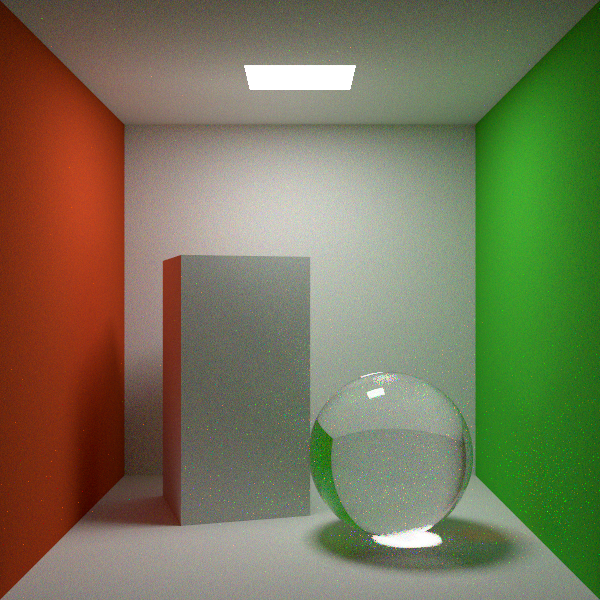
\includegraphics[width=\linewidth]{pt-cornell-box.png}\\[-2pt]
    \small\datei{cornell-box.rttf}
  \end{minipage}\hfill
  \begin{minipage}[b]{0.48\linewidth}\centering
    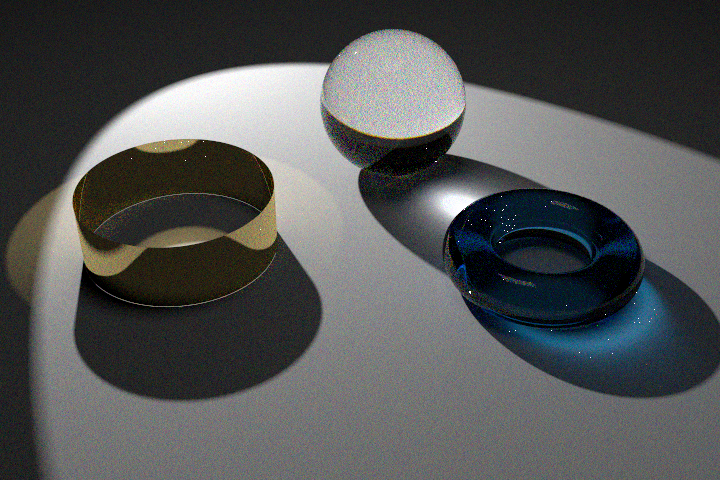
\includegraphics[width=\linewidth]{pt-caustics.png}\\[-2pt]
    \small\datei{caustics.rttf}
  \end{minipage}\\[8pt]
  \begin{minipage}[b]{0.48\linewidth}\centering
    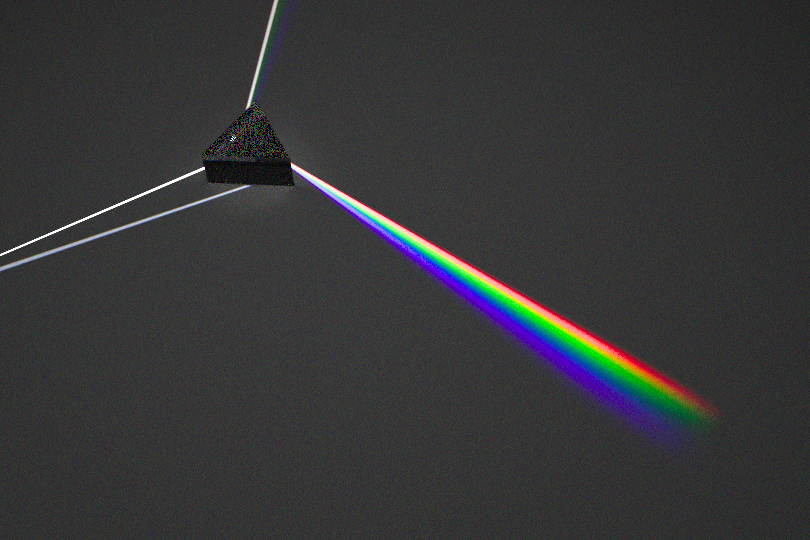
\includegraphics[width=\linewidth]{pt-prism.png}\\[-2pt]
    \small\datei{prism.rttf}
  \end{minipage}\hfill
  \begin{minipage}[b]{0.48\linewidth}\centering
    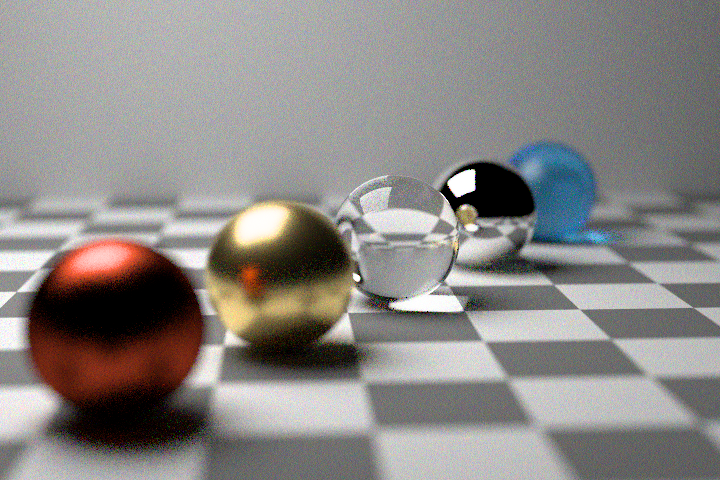
\includegraphics[width=\linewidth]{pt-depth-of-field.png}\\[-2pt]
    \small\datei{depth-of-field.rttf}
  \end{minipage}
  \caption{Farbbilder der vier Beispieldokumente des Path Tracers.}
  \label{fig:pt-beispiele}
\end{figure}

\begin{description}
  \item[\datei{cornell-box.rttf}] Ein Raum von \SI{550}{\milli\metre} mit roter und grüner Wand,
    einer Lampe in der Decke, einem Block und einer Glaskugel: Die Wände färben das Licht, das sie
    weitergeben; die Kugel wirft eine Kaustik. Reflexionsgrade je Wellenlänge, bidirektional.
  \item[\datei{caustics.rttf}] Ein Spot auf einem Tisch, eine Kugel aus stark dispergierendem Glas
    (Abbe-Zahl 28), ein Ring aus blauem Glas (Absorption je Wellenlänge) und ein Band aus poliertem
    Gold: Die Kugel sammelt das Licht in einem hellen Fleck mit farbigen Rändern, das Band erzeugt
    die herzförmige Kurve einer Kaffeetasse. Bidirektional.
  \item[\datei{prism.rttf}] Ein dünnes Band weißen Lichts streift einen Tisch und trifft ein Prisma
    aus Schwerflint ($n = 1{,}785$, Abbe-Zahl 25{,}7) unter dem Winkel minimaler Ablenkung: Die
    Farben verlassen es als Fächer, 31 Wellenlängen von 400 bis \SI{700}{\nano\metre}.
    Bidirektional.
  \item[\datei{depth-of-field.rttf}] Fünf Kugeln auf kariertem Boden unter weichem Licht -- roter
    Lack (glossy), gebürstetes Gold (metal), Glas, ein Spiegel und mattiertes blaues Glas --, durch
    eine Linse von \SI{14}{\milli\metre} Radius gesehen, scharf auf der Glaskugel. Path Tracing.
\end{description}

Die Dokumente verlangen 120 bis 160 Samples je Pixel. Mit dem C++-Kern dauert das auf einem
Laptop mit sechs Kernen etwa eine halbe Minute (Schärfentiefe) bis einige Minuten (Cornell-Box),
mit dem NumPy-Kern weit länger -- verringern Sie dort \gui{Samples} oder die Pixel der Kamera.

\section{Typische Arbeitsabläufe}\label{sec:pt-ablaeufe}

\subsection{Beleuchtungsstärke auf einem Arbeitstisch}

\begin{schritte}
  \item Konstruieren Sie Tisch, Raum (als Flächen oder Körper) und die Leuchtfläche der Leuchte.
  \item Ergänzen Sie die Quellentabelle: Name \code{leuchte}, \gui{Flux} 3000, \gui{in} \code{lm},
    \gui{Wavelengths / nm} z.\,B. \code{450:1, 550:2, 650:1}, \gui{Luminaire file} der Pfad der
    IES-Datei des Herstellers.
  \item Leuchtfläche auswählen, \gui{Source for the selection} = \code{leuchte},
    \gui{Selection: make it a source}.
  \item Wände und Decke: \code{white}; Boden: ein eigenes Material mit Reflexionsgrad 0{,}2.
  \item \gui{Show light paths}: Leuchtet die Leuchte nach unten? Wenn nicht: \gui{Side} auf
    \code{back} stellen.
  \item Tischplatte auswählen, bei \gui{Irradiance on} \gui{Use selection}.
  \item \gui{Results in} = \code{photometric (lm)}, \gui{Method} = \code{light tracing},
    \gui{Irradiance}. Die Tischplatte zeigt die Beleuchtungsstärke in lx, die Tabelle Mittel- und
    Höchstwert.
  \item Ist das Rauschen in der Tabelle zu groß, vervierfachen Sie \gui{Samples}.
\end{schritte}

\subsection{Ein Kamerabild einer Konstruktion}

\begin{schritte}
  \item Materialien zuweisen; eine große Fläche über der Szene als Quelle (\code{lamp}, Halbwinkel
    \SI{90}{\degree}).
  \item \gui{Position} und \gui{Looks at} mit \gui{Pick} setzen, \gui{Show camera} zur Kontrolle.
  \item Für eine erste Vorschau: \gui{Width} 160, \gui{Height} 120, \gui{Samples} 200\,000,
    \gui{Method} \code{path tracing}.
  \item \gui{Camera image}. Ist die Ansicht richtig, Pixel und Samples erhöhen.
  \item Enthält die Szene Glas oder Spiegel mit kleinen Quellen: \code{bidirectional}.
\end{schritte}

\subsection{Eine Kaustik hinter einer Linse}

\begin{schritte}
  \item Linse als geschlossener Körper, Material \code{BK7}.
  \item Kleine Quelle (z.\,B. ein Punkt oder eine kleine Fläche mit kleinem Halbwinkel) vor der
    Linse; mehrere Wellenlängen, wenn Farbfehler sichtbar werden sollen.
  \item Hinter der Linse eine Fläche mit Material \code{white} oder -- wenn sie das Licht nicht
    zurückwerfen soll -- \code{detector}.
  \item \gui{Irradiance on} = diese Fläche, \gui{Method} = \code{light tracing}, \gui{Texels}
    256, \gui{Irradiance}.
  \item Mit \gui{Also per wavelength} sehen Sie die Kaustik jeder Wellenlänge einzeln.
\end{schritte}

\subsection{Verfahren vergleichen}

\begin{schritte}
  \item Dieselbe Szene mit \code{light tracing} und \code{bidirectional} rechnen (gleiche Samples).
  \item In der Tabelle \enquote{Irradiance per face} die Flüsse vergleichen: Sie sollten innerhalb
    von etwa zwei Standardfehlern übereinstimmen.
  \item Weichen sie stärker ab, so findet eines der Verfahren bestimmte Pfade nicht
    (\autoref{sec:pt-verfahren}), oder \gui{Longest path} ist zu kurz.
\end{schritte}

\section{Fehlerbilder und Abhilfe}\label{sec:pt-fehler}

\begin{referenz}{@{}>{\raggedright\arraybackslash}p{0.4\linewidth} >{\raggedright\arraybackslash}X@{}}
\toprule
Meldung oder Beobachtung & Ursache und Abhilfe \\
\midrule\endhead
\texttt{Select surfaces or trimmed surfaces or shells first.} (bzw. mit \texttt{curves or points}) & Nichts Passendes ausgewählt. Objekte auswählen, dann die Aktion wiederholen. \\
\texttt{The material … is not in the table of materials.} & Der Name in \gui{Material for the selection} steht nicht in der Tabelle. \\
\texttt{The source … is not in the table of sources.} & Der Name in \gui{Source for the selection} steht nicht in der Tabelle. \\
\texttt{no object is a source: …} & Kein Objekt verweist auf eine Quelle. Objekt auswählen, \gui{Selection: make it a source}. \\
\textit{Objekt}\texttt{: its material … is not in the table of materials} & Material umbenannt oder gelöscht; neu zuweisen. \\
\texttt{the default material … is not in the table of materials} & \gui{Material of the other objects} nennt kein Material der Tabelle. \\
\texttt{sources need different, non-empty names} & Zwei Quellen heißen gleich oder eine hat keinen Namen. \\
\texttt{source …: a surface already belongs to another source} & Eine Fläche darf nur zu einer Quelle gehören. \\
\texttt{source … is on objects of different kinds …} & Eine Quelle auf Flächen \emph{und} Kurven/Punkten -- in zwei Quellen aufteilen. \\
\texttt{source …: a detector cannot be a source …} & Einer Leuchtfläche ist das Material \code{detector} zugewiesen. \\
\texttt{material …: reflectance + transmittance must lie in 0 … 1} & Werte der Zeile korrigieren. \\
\texttt{camera: position and target are the same point} & \gui{Position} und \gui{Looks at} unterscheiden sich nicht. \\
\texttt{camera: the view direction is parallel to the up direction} & Anderes \gui{Up} wählen. \\
\texttt{the model has no surfaces or bodies to trace} & Nur Kurven/Punkte im Modell oder alles inaktiv. \\
\texttt{luminaire file …: …} & Datei fehlt oder hat ein nicht unterstütztes Format (nur IES Typ C, EULUMDAT). \\
\texttt{The C++ kernel is not installed …} & Paket \code{pathtracer} installieren oder \gui{Kernel} = \code{automatic}. \\
Spiegel oder Glas im Kamerabild schwarz & \code{light tracing} erreicht eine Lochkamera nicht über Spiegel/Glas. \code{bidirectional} oder \code{path tracing} wählen. \\
Kaustik im Kamerabild fehlt, obwohl sie in der Textur zu sehen ist & Sie wird durch Glas oder im Spiegel gesehen: \code{photon mapping}. \\
Punktquelle im Kamerabild unsichtbar & Eine Lochkamera sieht Punktquellen nicht; \gui{Lens radius} $> 0$ und \code{light tracing} oder \code{bidirectional}. \\
Bild zu dunkel, nur einzelne helle Punkte & \gui{White at percentile} senken; mehr Samples. \\
Glaskörper verhält sich falsch & Körper nicht geschlossen; als geschlossenen Körper konstruieren. \\
Rechnung bricht mit Speichermangel ab & \gui{Processes} verringern (NumPy-Kern) oder den C++-Kern verwenden. \\
\bottomrule
\end{referenz}

\section{Grenzen}\label{sec:pt-grenzen}

\begin{itemize}
  \item Keine kontinuierlichen Spektren und Farben: Gerechnet wird mit einzelnen Linien.
  \item Keine gemessenen Materialien (BRDF-Daten).
  \item Quellen und Kameras dürfen nicht in Glas liegen.
  \item Ergebnisse werden nicht mit dem Dokument gespeichert; dafür gibt es \gui{Also write to
    file}.
  \item Kurven und Punkte als Quellen werfen keinen Schatten und sind für die Kamera unsichtbar.
\end{itemize}

% Kapitel: Das FourierGrating-Plugin (Beugungsgitter, RCWA / Fourier-Modal-Methode)
% Quellen: python/plugins/fouriergrating/ (fg_*.py, plugin.json, README.md), CHANGELOG.md,
% docs/adr/0010-multi-plugin-workflow.md
\chapter{Beugungsgitter mit FourierGrating}\label{kap:fouriergrating}
\index{FourierGrating}\index{Beugungsgitter}\index{RCWA}

Das Plugin \plugin{FourierGrating} berechnet die Beugung von Licht an periodischen Strukturen:
Liniengitter, Kreuzgitter, Schichtstapel mit Lamellen, Profilen oder beliebig geformten
Einschlüssen. Es verbindet \produkt{} mit dem Rechenkern \emph{FourierGrating}, einer
Implementierung der rigorosen Kopplungswellenanalyse (RCWA, auch Fourier-Modal-Methode genannt)
und der differentiellen Methode. Alles, was Sie für ein Gitter einstellen -- Struktur,
Materialien, Schichten, Beleuchtung --, steht im Panel \gui{Plugin}; die Ergebnisse erscheinen als
Tabellen, Balken, Kurven und Bilder in den Ergebnisfenstern der Anwendung.

Das Kapitel beschreibt das Plugin aus Anwendersicht: zuerst das Gittermodell mit seinen
Koordinaten, dann Materialien, Schichten und Beleuchtung, anschließend die Rechnungen (Einzelrechnung,
Scan, Aufwandsschätzung, Optimierung), das Nahfeld, Schichten aus CAD-Körpern und das Gitter als Block
im Node-Workflow. Den Abschluss bilden Arbeitsabläufe Schritt für Schritt, typische Fehler und die
Grenzen des Plugins. Die vollständige Liste aller Parameter mit Standardwerten und Wertebereichen
steht im Anhang, \autoref{kap:plugin-fouriergrating}.

\section{Überblick}\label{sec:fg-ueberblick}

\subsection{Was das Plugin kann}

\begin{itemize}
  \item \textbf{Einzelrechnung} (\gui{Solve}): die Beugungseffizienz jeder reflektierten und
    transmittierten Ordnung, die Summen $\Sigma R$ und $\Sigma T$, die Absorption und die
    Energiebilanz.
  \item \textbf{Scan} (\gui{Scan}): dieselben Größen über Listen oder Bereiche der Wellenlänge,
    der Einfallswinkel, der Polarisation und über einen beliebigen Zahlenwert der Konfiguration
    (Sweep), als Kurven.
  \item \textbf{Aufwandsschätzung} (\gui{Estimate}): Zahl der Rechnungen, Matrixgröße und grober
    Speicherbedarf, bevor Sie eine große Rechnung starten.
  \item \textbf{Optimierung} (\gui{Optimise}): Schichtdicken, Lamellenkanten, Perioden oder andere
    Zahlen der Konfiguration so wählen, dass eine gewichtete Summe von Effizienzen maximal oder
    minimal wird -- mit den exakten Gradienten von FourierGrating.
  \item \textbf{Littrow-Winkel} (\gui{Set Littrow angle}): den Einfallswinkel, unter dem eine
    reflektierte Ordnung in die Einfallsrichtung zurückläuft.
  \item \textbf{Nahfeld} (\gui{Near field}): das elektromagnetische Feld im und am Gitter als
    Bilder und Kurven.
  \item \textbf{Schichten aus CAD-Körpern} (\gui{Layer from CAD bodies}, \gui{Check CAD layers}):
    eine im CAD gezeichnete Elementarzelle als Gitterschicht.
  \item \textbf{Konfigurationsdateien} (\gui{Load configuration}, \gui{Save configuration}): das
    JSON-Format von FourierGrating lesen und schreiben, verlustfrei.
  \item \textbf{Blöcke für den Node-Workflow}: das Gitter \block{fg.grating} und den Schichtstapel
    \block{fg.stack}, die Strahlen und Felder im optischen Aufbau beugen bzw. filtern.
\end{itemize}

\subsection{Voraussetzungen}\label{sec:fg-voraussetzungen}
\index{fouriergrating (Python-Paket)}

Das Plugin wird mit der Anwendung installiert (Plugin-Kennung \code{fg}, Name
\plugin{FourierGrating}). Es braucht in der Python-Umgebung der Plugins die Pakete
\code{numpy}, \code{scipy} und \code{fouriergrating} in Version 0.18 oder neuer. Der Knopf
\gui{Create environment…} in \menu{Plugins,Settings…} installiert sie (siehe
\autoref{kap:installation} und \autoref{kap:plugins}). Fehlt das Paket \code{fouriergrating}, meldet
jede rechnende Aktion:

\begin{lstlisting}
The FourierGrating plugin needs the Python package fouriergrating in the plugin environment
(pip install fouriergrating, or the wheel of the FourierGrating repo).
\end{lstlisting}

Laden und Speichern von Konfigurationen, das Bearbeiten im Panel, \gui{Estimate} und
\gui{Set Littrow angle} funktionieren auch ohne das Paket. Zwei Funktionen haben weitere
Voraussetzungen:

\begin{itemize}
  \item \gui{Layer from CAD bodies} und \gui{Check CAD layers} brauchen ein \code{fouriergrating}
    mit CAD-Slicer (ein Build mit \code{FG\_ENABLE\_NURBFORGE}, siehe die Datei \datei{docs/cad.md}
    von FourierGrating). Ohne ihn wird die Schicht zwar angelegt, aber nicht geprüft.
  \item Die Workflow-Blöcke \block{fg.grating} und \block{fg.stack} stellt das Plugin nur bereit,
    wenn das Paket \code{rtt-fusion} mit Fernblöcken installiert ist (Modul
    \code{rtt\_fusion.graph.remote}).
\end{itemize}

\subsection{Wo Sie das Plugin finden}

\begin{itemize}
  \item Im Menü \menu{Plugins,FourierGrating} stehen alle Aktionen (alphabetisch nach ihrem
    internen Namen geordnet).
  \item In der Werkzeugspalte bildet das Plugin eine eigene Gruppe \gui{FourierGrating} mit einem
    Knopf je Aktion.
  \item Im Dock \gui{Plugin} wählen Sie oben \gui{FourierGrating}; darunter stehen die Parameter,
    unten die Knöpfe der Aktionen und \gui{Reset parameters} (setzt alle Parameter auf ihre
    Standardwerte zurück).
  \item Zwei Aktionen gelten einem einzelnen Block des Node-Workflows. Sie stehen nicht im Menü,
    sondern im Kontextmenü eines Gitter- oder Stapelblocks im Node-Editor
    (\autoref{sec:fg-block}).
\end{itemize}

Die Parameter werden mit dem Dokument gespeichert (pro Plugin). Ein geänderter Parameter markiert
das Dokument als geändert, ist aber kein Rückgängig-Schritt.

\subsection{Aufbau des Panels}\label{sec:fg-panel}

Das Panel ist in Gruppen gegliedert. Ganz oben stehen ohne eigenen Rahmen die beiden Listen
\gui{Materials} und \gui{Layers (bottom to top)}, darunter die Gruppenkästen in dieser
Reihenfolge:

\begin{referenz}{>{\raggedright\arraybackslash}p{3.2cm}>{\raggedright\arraybackslash}X}
\toprule
Gruppe & Inhalt \\
\midrule
\endhead
(ohne Gruppe) & \gui{Materials} (Liste der Materialien), \gui{Layers (bottom to top)} (Schichtstapel) \\
\gui{File} & \gui{Configuration} (Datei zum Laden), \gui{Save as} (Datei zum Speichern) \\
\gui{Structure} & \gui{Dimension}, \gui{Solver}, \gui{Orders Nx}, \gui{Orders Nz}, \gui{Period x},
  \gui{Period z}, \gui{Superstrate}, \gui{Substrate}, \gui{Solve: also write CSV} \\
\gui{Incidence} & \gui{$\lambda$ / \si{\micro\metre}}, \gui{$\varphi$ / deg}, \gui{$\psi$ / deg},
  \gui{$\delta$ / deg}, \gui{Littrow order} \\
\gui{Scan} & \gui{x axis}, \gui{Orders from efficiency}, \gui{At most curves}, \gui{Also write CSV} \\
\gui{Near field} & \gui{Show}, \gui{y from}, \gui{y to}, \gui{Horizontal cut at y},
  \gui{Vertical cut at z (2D)}, \gui{Points x}, \gui{Points y}, \gui{Points z (2D)}, \gui{Periods},
  \gui{Also write .npz} \\
\gui{Optimisation} & \gui{Goal}, \gui{Objective L = $\Sigma$ weight $\cdot$ efficiency},
  \gui{Parameters}, \gui{Iterations}, \gui{Apply the optimum to the panel} \\
\gui{CAD layer} & \gui{Bodies}, \gui{Bodies drawn in}, \gui{STEP file}, \gui{Around the bodies},
  \gui{RCWA slices per band}, \gui{Preview at height}, \gui{Preview SVG} \\
\gui{Advanced} & \gui{Further settings (JSON)}: alle übrigen Schlüssel der Konfiguration \\
\bottomrule
\end{referenz}

Fahren Sie mit der Maus über ein Feld, zeigt ein Tooltip seine Kurzbeschreibung. Ungültige
Eingaben (etwa fehlerhaftes JSON oder eine falsche Tabellenzelle) werden rot markiert und sperren
die Aktionen, bis sie behoben sind.

\subsection{Wo die Ergebnisse erscheinen}

Jede rechnende Aktion legt im Dock \gui{Results} einen neuen Ergebnissatz an (etwa
\enquote{FourierGrating $\lambda$ = 0.6328 \si{\micro\metre}}). Ergebnissätze lassen sich
ein- und ausblenden, vergleichen und löschen; sie werden mit dem Dokument gespeichert. Die
einzelnen Ergebnisse landen je nach Art in

\begin{itemize}
  \item dem Fenster \gui{Table} (Ordnungstabelle, Parameter der Optimierung, Bänder und Befunde der
    CAD-Prüfung),
  \item dem Fenster \gui{Plot} (Balken der Effizienzen, Kurven des Scans und der Optimierung,
    horizontaler Nahfeldschnitt eines 1D-Gitters),
  \item dem Fenster \gui{Image} (Nahfeldschnitte als Farbbilder),
  \item dem Dock \gui{Plugin log} (Summen, Energiebilanz, Warnungen, Schritte der Optimierung) und
  \item der Statusleiste (eine Zusammenfassung nach dem Ende der Aktion).
\end{itemize}

Ein Fehler, den Sie selbst beheben können -- eine fehlende Datei, ein unbekanntes Material --,
erscheint als Meldungsfenster mit dem Text des Plugins. Alle anderen Fehler stehen mit
Einzelheiten im \gui{Plugin log}. Eine laufende Aktion brechen Sie mit dem Knopf \gui{Cancel} in der
Statusleiste ab.

\begin{hinweis}
Eine einzelne Rechnung von FourierGrating, die bereits läuft, lässt sich nicht mittendrin
unterbrechen. \gui{Optimise} prüft den Abbruch zwischen zwei Auswertungen; bei \gui{Solve},
\gui{Scan} und \gui{Near field} wirkt \gui{Cancel} erst, wenn die Rechnung zurückkehrt -- oder die
Anwendung beendet den Plugin-Prozess nach einigen Sekunden. Schätzen Sie große Rechnungen deshalb
vorher mit \gui{Estimate} ab (\autoref{sec:fg-estimate}).
\end{hinweis}

% ---------------------------------------------------------------------------------------------
\section{Das Gittermodell}\label{sec:fg-modell}
\index{Gittermodell}

\subsection{Koordinaten und Schichtung}\label{sec:fg-koordinaten}

FourierGrating beschreibt ein Gitter als Stapel von Schichten zwischen zwei Halbräumen:

\begin{itemize}
  \item Die \textbf{y-Achse} ist die Stapelrichtung. Unten liegt das \textbf{Substrat}
    ($y < 0$), oben das \textbf{Superstrat}. Die Schichten liegen dazwischen, die unterste beginnt
    bei $y = 0$.
  \item Das Licht fällt \textbf{von oben}, aus dem Superstrat, ein. Reflektierte Ordnungen laufen
    zurück ins Superstrat (Seite \code{R}), transmittierte ins Substrat (Seite \code{T}).
  \item Die Struktur ist periodisch in \textbf{x} mit der Periode $\Lambda_x$ (\gui{Period x}),
    bei einem Kreuzgitter (2D) zusätzlich in \textbf{z} mit $\Lambda_z$ (\gui{Period z}).
  \item Alle Längen sind in Mikrometern (\si{\micro\metre}), alle Winkel in Grad.
\end{itemize}

Diese Konvention gilt im ganzen Plugin: im Panel, in den Konfigurationsdateien, beim Nahfeld
(\gui{y from}/\gui{y to} zählen ab der Unterkante des Stapels) und bei den CAD-Schichten (dort
wird die CAD-Achse $+Z$ zur Stapelrichtung $y$, siehe \autoref{sec:fg-cad}).

\subsection{Dimension: Liniengitter und Kreuzgitter}

\gui{Dimension} wählt zwischen
\begin{description}
  \item[\code{1D}] einem Liniengitter: periodisch nur in x, unendlich ausgedehnt und konstant in z.
    Die Ordnungen tragen einen Index $n$.
  \item[\code{2D}] einem Kreuzgitter: periodisch in x und z. Die Ordnungen tragen zwei Indizes
    $(n, m)$; \gui{Period z} muss dann größer als null sein.
\end{description}

Lamellen- und isotrope Profilschichten eines Liniengitters sind auch in einem 2D-Stapel erlaubt;
sie sind dann in z konstant.

\subsection{Fourier-Ordnungen und Matrixgröße}\label{sec:fg-ordnungen}
\index{Fourier-Ordnungen}\index{Abbruch (Truncation)}

Die Methode entwickelt Feld und Material in Fourier-Reihen. \gui{Orders Nx} und \gui{Orders Nz}
legen fest, wie viele Glieder mitgenommen werden: von $-N_x$ bis $+N_x$ in x und von $-N_z$ bis
$+N_z$ in z. Die Zahl der Fourier-Glieder ist
\[
  n_f = 2N_x + 1 \quad\text{(1D)}, \qquad n_f = (2N_x + 1)(2N_z + 1) \quad\text{(2D)},
\]
und die Matrix des Eigenwertproblems hat die Größe $n = 4 n_f$. Rechenzeit und Speicher wachsen
mit $n^3$ bzw. $n^2$ -- ein 2D-Gitter mit $N_x = N_z = 10$ hat $n = 1764$, ein 1D-Gitter mit
$N_x = 10$ nur $n = 84$.

\begin{tipp}
Prüfen Sie die Konvergenz: rechnen Sie mit $N_x$, dann mit einem deutlich größeren Wert (etwa dem
Doppelten). Ändern sich die Effizienzen, die Sie interessieren, nicht mehr in den benötigten
Stellen, reicht der kleinere Wert. Metallische Lamellen in TM-Polarisation konvergieren langsam und
brauchen viele Ordnungen.
\end{tipp}

Die Standardwerte sind $N_x = 10$ und $N_z = 0$, der erlaubte Bereich 0 bis 200.

\subsection{Rechenverfahren}\label{sec:fg-solver}
\index{differentielle Methode}

\gui{Solver} wählt das Verfahren:
\begin{description}
  \item[\code{rcwa}] die RCWA (Fourier-Modal-Methode): jede Schicht wird in y in Scheiben
    konstanter Struktur zerlegt, in jeder Scheibe wird ein Eigenwertproblem gelöst. Für
    Lamellen- und homogene Schichten ist das exakt; Profile werden durch Scheiben angenähert.
    Die Scheibenzahl regelt der Schlüssel \code{rcwa} unter \gui{Advanced}
    (\code{\{\textquotedbl{}rcwa\textquotedbl{}: \{\textquotedbl{}slices\textquotedbl{}: 60\}\}}) bzw. \code{slices} der einzelnen Profilschicht.
  \item[\code{rk}] die differentielle Methode: das Feld wird mit einem impliziten
    Runge-Kutta-Verfahren durch die Schicht integriert. Sie eignet sich für stetig veränderliche
    Profile. Einstellungen (Tableau, Toleranz) stehen ebenfalls unter \gui{Advanced}
    (Schlüssel \code{rk}).
\end{description}

\subsection{Superstrat und Substrat}

\gui{Superstrate} und \gui{Substrate} nennen die Materialien der beiden Halbräume -- über ihren
Namen in der Materialliste (Standard: \code{air} und \code{glass}). Ein Name, der in der Liste
fehlt, führt beim Rechnen zu einer Meldung von FourierGrating.

\begin{warnung}
Das Superstrat muss verlustfrei sein (reelle Brechzahl), denn aus ihm fällt das Licht ein.
FourierGrating prüft das beim Laden der Konfiguration.
\end{warnung}

\subsection{Gittergleichung und Ordnungen}\label{sec:fg-gittergleichung}
\index{Gittergleichung}

Für eine ebene Welle aus dem Superstrat mit der Brechzahl $\nu$ unter dem Polarwinkel $\varphi$
(gemessen gegen die y-Achse, also gegen die Flächennormale) und dem Azimut $\psi$ (gemessen gegen
x) lautet die x-Komponente des normierten Wellenvektors der Ordnung $n$
\[
  \alpha_n = \nu \sin\varphi \cos\psi + n\,\frac{\lambda}{\Lambda_x},
\]
in 2D zusätzlich $\gamma_m = \nu \sin\varphi \sin\psi + m\,\lambda/\Lambda_z$. Eine Ordnung
breitet sich in einem Medium mit der Brechzahl $n_\text{M}$ nur aus, wenn
$\alpha_n^2 + \gamma_m^2 < n_\text{M}^2$; sonst ist sie evaneszent und trägt keine Leistung fort.
Deshalb hängt die Zahl der Zeilen in der Ordnungstabelle von $\lambda$, $\Lambda$ und den Winkeln
ab, und im Scan kann eine Ordnung an manchen Punkten fehlen.

% ---------------------------------------------------------------------------------------------
\section{Materialien}\label{sec:fg-materialien}
\index{Material (FourierGrating)}\index{Brechzahl}

Die Liste \gui{Materials} enthält alle Materialien, auf die sich Superstrat, Substrat und Schichten
beziehen. Standardmäßig stehen dort \code{air} ($n = 1$) und \code{glass} ($n = 1{,}5$).

\subsection{Materialien bearbeiten}

Die Liste hat die Knöpfe \gui{Add} (neuer Eintrag), \gui{Edit…} (öffnet den Eintrag in einem
Dialog \gui{Edit entry}), \gui{Remove}, $\uparrow$ und $\downarrow$ (Reihenfolge ändern). Ein
Eintrag hat diese Felder:

\begin{description}
  \item[\gui{Name}] der Name, unter dem Schichten, Superstrat und Substrat das Material nennen.
    Groß- und Kleinschreibung zählt.
  \item[\gui{Given as}] \code{n} -- die komplexe Brechzahl $n + \mathrm{i}k$ aus den Feldern
    \gui{n} und \gui{k}; \code{json} -- jede andere Form, die FourierGrating kennt, als JSON im
    Feld \gui{Material as JSON (json)}.
  \item[\gui{n}, \gui{k}] Real- und Imaginärteil der Brechzahl. $k > 0$ bedeutet Absorption.
    Ist $k = 0$, wird das Material als reelle Zahl gespeichert, sonst als Paar \code{[n, k]}.
\end{description}

\subsection{Weitere Materialformen (JSON)}

Mit \gui{Given as} = \code{json} geben Sie das Material so ein, wie es in der Konfigurationsdatei
unter seinem Namen stünde. FourierGrating kennt unter anderem (Format nach seiner Dokumentation
\datei{docs/config\_format.md}):

\begin{itemize}
  \item einen vollständigen Permittivitätstensor (\code{eps\_tensor}) für anisotrope Materialien,
  \item Hauptachsenwerte mit Euler-Winkeln (\code{eps\_principal}, \code{euler\_deg}),
  \item dispersive Modelle, die an jeder Wellenlänge eines Scans ausgewertet werden: Sellmeier,
    Cauchy, Drude-Lorentz und Tabellen.
\end{itemize}

Ein Beispiel: Quarzglas nach Sellmeier.

\begin{lstlisting}
{ "n": { "sellmeier": { "A": 1.0, "B": [0.6961663, 0.4079426, 0.8974794],
                        "C_um2": [0.00467914826, 0.0135120631, 97.9340025] } } }
\end{lstlisting}

Materialien, die Sie als JSON eingeben, reicht das Plugin unverändert an FourierGrating weiter; beim
Laden einer Datei landen alle Materialien, die keine einfache Brechzahl sind, automatisch in dieser
Form im Panel.

\begin{hinweis}
\gui{Set Littrow angle} braucht die Brechzahl des Superstrats als Zahl. Ist das Superstrat als JSON
gegeben, meldet die Aktion \enquote{the superstrate … needs a refractive index n (not JSON)}.
\end{hinweis}

% ---------------------------------------------------------------------------------------------
\section{Der Schichtstapel}\label{sec:fg-schichten}
\index{Schichtstapel}\index{Lamellengitter}

Die Liste \gui{Layers (bottom to top)} beschreibt die Schichten zwischen Substrat und Superstrat --
\textbf{von unten nach oben}: der erste Eintrag liegt direkt auf dem Substrat, der letzte grenzt an
das Superstrat. Das ist auch die Zählung der JSON-Zeiger: \code{/layers/0} ist die unterste
Schicht. Mit $\uparrow$ und $\downarrow$ verschieben Sie eine Schicht im Stapel. Ein leerer Stapel
ist erlaubt: dann rechnet FourierGrating die ebene Grenzfläche zwischen Superstrat und Substrat.

Jeder Eintrag hat einen \gui{Type}; die übrigen Felder gelten je nach Typ.

\subsection{Homogene Schicht}

\gui{Type} = \code{homogeneous}: eine ebene Schicht der Dicke \gui{Thickness} (in
\si{\micro\metre}) aus dem Material \gui{Material (homogeneous)}. Damit bauen Sie Beschichtungen,
Zwischenschichten und Deckschichten.

\subsection{Lamellenschicht}\label{sec:fg-lamellen}

\gui{Type} = \code{lamellar1d}: eine Schicht der Dicke \gui{Thickness}, die in x aus Lamellen
verschiedener Materialien besteht -- das klassische binäre Gitter. Die Lamellen stehen in der
Tabelle \gui{Lamellae (lamellar1d)} mit den Spalten \gui{from x} (Beginn der Lamelle in
\si{\micro\metre}) und \gui{material}. Jede Lamelle reicht von ihrem \gui{from x} bis zum
\gui{from x} der nächsten Zeile, die letzte bis \gui{End (lamellar1d)}. Zeilen fügen Sie mit
\gui{Add row} an und löschen sie mit \gui{Remove row}.

Ein Gitter mit Periode \qty{1}{\micro\metre}, dessen erste Hälfte Glas und zweite Hälfte Luft ist:

\begin{center}
\begin{tabular}{rl}
\toprule
\gui{from x} & \gui{material} \\
\midrule
0.0 & glass \\
0.5 & air \\
\bottomrule
\end{tabular}
\qquad \gui{End (lamellar1d)} = 1.0
\end{center}

In der Konfigurationsdatei wird daraus \code{\textquotedbl{}breakpoints\_um\textquotedbl{}: [0.0, 0.5, 1.0]} und
\code{\textquotedbl{}materials\textquotedbl{}: [\textquotedbl{}glass\textquotedbl{}, \textquotedbl{}air\textquotedbl{}]}.

\begin{warnung}
Die Kanten müssen bei 0 beginnen und genau bei der Periode $\Lambda_x$ enden: die erste Zeile hat
\gui{from x} = 0, \gui{End} ist gleich \gui{Period x}. FourierGrating prüft das
\textbf{nicht}. Ändern Sie die Periode, ohne \gui{End} anzupassen, ist das Ergebnis ohne Meldung
falsch.
\end{warnung}

\subsection{Profile und weitere Schichttypen (JSON)}\label{sec:fg-profile}
\index{Profilgitter}

\gui{Type} = \code{json}: jede andere Schicht von FourierGrating, eingegeben im Feld
\gui{Layer as JSON (type json)} genau so, wie sie in der Konfigurationsdatei unter
\code{layers} stünde. Laut der Formatbeschreibung von FourierGrating gibt es unter anderem:

\begin{description}
  \item[\code{profile1d}] ein stetiges Oberflächenprofil eines Liniengitters zwischen zwei
    Materialien (\code{below}, \code{above}) mit der Tiefe \code{depth\_um}. Formen:
    \code{sinus}, \code{triangle} (Dreieck mit der Spitze bei \code{apex\_x\_um}) und
    \code{points} (Stützstellen \code{x\_um}, \code{y\_um}, stückweise linear).
  \item[\code{profile2d}] ein Profil eines Kreuzgitters (\code{egg\_crate}, \code{sinus\_x}).
  \item[\code{polygon2d}] eine Schicht eines Kreuzgitters mit polygonalen oder rechteckigen
    Einschlüssen in einem Hintergrundmaterial.
  \item[\code{contour2d}] Einschlüsse mit gekrümmten Rändern: Kreise, Ellipsen, Polygone,
    NURBS-Konturen, auch mit Löchern.
  \item[\code{cad}] Körper aus einer STEP-Datei, die FourierGrating in Bänder zerlegt -- diese
    Schicht legt das Plugin für Sie an (\autoref{sec:fg-cad}).
\end{description}

Ein sinusförmiges Reliefgitter in Aluminium unter Luft, \qty{0.2}{\micro\metre} tief:

\begin{lstlisting}
{ "type": "profile1d", "shape": "sinus", "depth_um": 0.2,
  "below": "al", "above": "air", "slices": 0, "factorization": "auto" }
\end{lstlisting}

Das Plugin prüft den Inhalt eines JSON-Eintrags nicht selbst; Fehler meldet FourierGrating beim
Rechnen (\enquote{FourierGrating: …}). Ungültiges JSON markiert das Feld rot.

\begin{tipp}
Wenn Sie eine Konfigurationsdatei mit solchen Schichten laden, zeigt das Panel sie als Einträge vom
Typ \code{json}; nur homogene und Lamellenschichten in genau der einfachen Form erscheinen als
Felder. Beim Speichern wird jede Schicht wieder so geschrieben, wie sie war.
\end{tipp}

% ---------------------------------------------------------------------------------------------
\section{Beleuchtung und Polarisation}\label{sec:fg-beleuchtung}
\index{Polarisation}\index{Einfallswinkel}

Die Gruppe \gui{Incidence} beschreibt die einfallende ebene Welle:

\begin{description}
  \item[\gui{$\lambda$ / \si{\micro\metre}}] die Vakuumwellenlänge in Mikrometern
    (Standard 0.6328, die Linie des HeNe-Lasers).
  \item[\gui{$\varphi$ / deg}] der Polarwinkel des Einfalls gegen die Flächennormale (die
    y-Achse). $\varphi = 0$ ist senkrechter Einfall.
  \item[\gui{$\psi$ / deg}] der Azimut der Einfallsebene gegen die x-Achse. $\psi = 0$: die
    Einfallsebene steht senkrecht auf den Gitterlinien eines Liniengitters (klassische
    Anordnung); $\psi \neq 0$: konischer Einfall.
  \item[\gui{$\delta$ / deg}] der Polarisationswinkel: \code{0} ist s-Polarisation (TE),
    \code{90} p-Polarisation (TM).
\end{description}

\subsection{Zahl, Liste oder Bereich}\label{sec:fg-scan-syntax}

Jedes der vier Felder nimmt eine von drei Formen an:

\begin{center}
\begin{tabularx}{\linewidth}{ll>{\raggedright\arraybackslash}X}
\toprule
Form & Eingabe & Bedeutung \\
\midrule
Zahl & \code{0.6328} & ein Wert \\
Liste & \code{0.5, 0.6, 0.7} & die genannten Werte \\
Bereich & \code{0.5:0.7:21} & von 0,5 bis 0,7 in 21 gleichen Schritten (beide Enden eingeschlossen) \\
\bottomrule
\end{tabularx}
\end{center}

Schreiben Sie Dezimalzahlen in diesen Feldern immer mit Punkt. Eine Liste trennen Sie mit
Kommas, einen Bereich mit Doppelpunkten in der Reihenfolge \code{von:bis:Schritte}.

Mehrere Listen und Bereiche ergeben einen Scan über das \textbf{kartesische Produkt}: drei
Wellenlängen und zwei Polarisationen sind sechs Rechenpunkte. \gui{Scan} rechnet alle Punkte;
\gui{Solve}, \gui{Near field} und \gui{Optimise} rechnen nur den \textbf{ersten} Punkt (die erste
Wellenlänge, den ersten Winkel, die erste Polarisation).

\begin{hinweis}
Ein leeres Feld lässt den Schlüssel in der Konfiguration weg. FourierGrating setzt dann seinen
eigenen Standard ein. Die Wellenlänge sollten Sie immer angeben.
\end{hinweis}

\section{Littrow-Anordnung}\label{sec:fg-littrow}
\index{Littrow-Anordnung}

In der Littrow-Anordnung läuft eine reflektierte Beugungsordnung genau in die Einfallsrichtung
zurück -- typisch für Gitter in Laserresonatoren und Spektrometern. Für die Ordnung $n$ gilt dann
$\alpha_n = -\alpha_0$, also
\[
  \sin\varphi = -\frac{n\,\lambda}{2\,\Lambda_x\,\nu\,\cos\psi}.
\]
Dabei ist $\nu$ die Brechzahl des Superstrats, $\lambda$ die erste Wellenlänge und $\psi$ der erste
Azimut des Panels.

\begin{schritte}
  \item Tragen Sie in der Gruppe \gui{Incidence} unter \gui{Littrow order} die gewünschte Ordnung
    ein (Standard $-1$, erlaubt $-50$ bis $50$).
  \item Wählen Sie \menu{Plugins,FourierGrating,Set Littrow angle} oder den gleichnamigen Knopf.
  \item Das Plugin schreibt den Winkel in das Feld \gui{$\varphi$ / deg} (mit zehn gültigen
    Stellen) und meldet ihn in der Statusleiste, etwa \enquote{$\varphi$ = 18.4454\si{\degree} (Littrow, order -1)}.
\end{schritte}

Beispiel: $\lambda = \qty{0.6328}{\micro\metre}$, $\Lambda_x = \qty{1}{\micro\metre}$, Luft
($\nu = 1$), $\psi = 0$, Ordnung $-1$: $\sin\varphi = 0{,}3164$, also
$\varphi \approx \ang{18.45}$.

Die Aktion meldet einen Fehler, wenn \gui{Period x} nicht größer als null ist, wenn das Superstrat
nicht als Brechzahl gegeben ist, oder wenn die Ordnung keinen Littrow-Winkel hat (Ordnung 0 oder
$|\sin\varphi| > 1$, die Meldung nennt den Wert).

\begin{tipp}
\gui{Set Littrow angle} überschreibt das Feld \gui{$\varphi$ / deg} mit einer einzelnen Zahl; ein
vorher eingetragener Bereich ist danach weg.
\end{tipp}

% ---------------------------------------------------------------------------------------------
\section{Rechnen}\label{sec:fg-rechnen}

\subsection{Einzelrechnung: Solve}\label{sec:fg-solve}
\index{Beugungseffizienz}

\gui{Solve} rechnet die Konfiguration des Panels für den ersten Punkt der Beleuchtung und zeigt die
Effizienzen aller Ordnungen, die sich im Superstrat oder Substrat ausbreiten.

\begin{schritte}
  \item Stellen Sie Struktur, Materialien, Schichten und Beleuchtung ein.
  \item Wählen Sie \menu{Plugins,FourierGrating,Solve} oder den Knopf \gui{Solve} im Panel.
  \item Die Statusleiste zeigt \enquote{solving …}, nach dem Ende eine Zusammenfassung der Form (die Zahlen hier nur als Beispiel)
    \enquote{FourierGrating: $\Sigma$R 0.0400, $\Sigma$T 0.9600, A 0.0000 (8 orders)}.
\end{schritte}

Das Ergebnis besteht aus

\begin{description}
  \item[Tabelle \enquote{Orders}] im Fenster \gui{Table}, eine Zeile je Ordnung mit den Spalten
    \code{side} (\code{R} reflektiert, \code{T} transmittiert), \code{n}, \code{m} (in 1D immer 0),
    \code{efficiency}, \code{s part} und \code{p part}. Die Effizienz ist der Anteil der einfallenden
    Leistung, den die Ordnung fortträgt; \code{s part} und \code{p part} teilen ihn auf die beiden
    Polarisationen der gebeugten Welle auf (in isotropen Medien).
  \item[Balken \enquote{Efficiency per order}] im Fenster \gui{Plot}: je Ordnung ein Balken,
    beschriftet \code{R 0}, \code{R -1}, \code{T 1} usw. (in 2D \code{R 1,0}).
  \item[Protokollzeile] im \gui{Plugin log}: $\Sigma R$, $\Sigma T$, die Absorption $A$ und,
    wenn FourierGrating sie liefert, die Energiebilanz; davor jede Warnung von FourierGrating
    (\enquote{warning: …}).
\end{description}

Der Ergebnissatz heißt nach der Wellenlänge, etwa \enquote{FourierGrating $\lambda$ = 0.6328
\si{\micro\metre}}; bei einer Liste steht die ganze Liste im Namen, gerechnet wird trotzdem nur
der erste Punkt.

\paragraph{Energiebilanz.} Für ein verlustfreies Gitter (alle $k = 0$) muss
$\Sigma R + \Sigma T = 1$ sein, $A = 0$. Weicht die Summe merklich ab, ist die Rechnung nicht
konvergiert oder falsch eingestellt (zu wenige Ordnungen, zu wenige Scheiben, falsche
Lamellenkanten). Mit absorbierenden Materialien ist $A = 1 - \Sigma R - \Sigma T > 0$.

\paragraph{Als CSV schreiben.} Steht in \gui{Solve: also write CSV} (Gruppe \gui{Structure}) eine
Datei, schreibt \gui{Solve} die Ordnungstabelle zusätzlich dorthin -- mit den Spalten
\code{side, n, m, efficiency, eff\_s, eff\_p}. Das Protokoll meldet \enquote{\dots{} orders written to
\dots}. Lassen Sie das Feld leer, wenn Sie keine Datei wollen.

\subsection{Parameterscan: Scan}\label{sec:fg-scan}
\index{Scan (FourierGrating)}\index{Sweep}

\gui{Scan} rechnet \emph{alle} Punkte der Listen und Bereiche in der Gruppe \gui{Incidence} und
eines Sweeps -- parallel, in FourierGrating -- und zeigt die Effizienzen als Kurven.

\paragraph{Was gescannt wird.}
\begin{itemize}
  \item Die vier Felder der Beleuchtung: jede Liste oder jeder Bereich (\autoref{sec:fg-scan-syntax}).
    Mehrere variierende Größen ergeben das kartesische Produkt.
  \item Ein \textbf{Sweep} über eine beliebige Zahl der Konfiguration, etwa eine Schichtdicke.
    Ihn tragen Sie unter \gui{Advanced} in \gui{Further settings (JSON)} ein:
\begin{lstlisting}
{ "sweep": { "parameter": "/layers/0/thickness_um",
             "values": { "from": 0.1, "to": 0.3, "steps": 11 } } }
\end{lstlisting}
    \code{parameter} ist ein JSON-Zeiger in die Konfiguration (\autoref{sec:fg-zeiger}),
    \code{values} eine Zahl, eine Liste oder ein Bereich. Die Sweep-Werte laufen nacheinander, die
    Punkte jedes Werts parallel.
\end{itemize}

Gibt es nur einen einzigen Punkt, meldet \gui{Scan}: \enquote{the scan has a single point – give a
list or a range for $\lambda$, an angle or a sweep}.

\paragraph{Die Kurven.} Im Fenster \gui{Plot} erscheinen
\begin{itemize}
  \item $\Sigma R$ und $\Sigma T$ über der x-Achse,
  \item jede Ordnung, deren Effizienz irgendwo den Wert \gui{Orders from efficiency} erreicht
    (Standard 0,01), als eigene Kurve, benannt \code{R 0}, \code{T -1} (in 2D \code{R 1,0}).
\end{itemize}

Die x-Achse wählt \gui{x axis}: \code{auto} nimmt die Größe mit den meisten Werten (bei Gleichstand
zuerst $\lambda$); \code{lambda\_um}, \code{phi\_deg}, \code{psi\_deg}, \code{delta\_deg} oder
\code{sweep\_value} erzwingen eine bestimmte. Variiert die gewählte Größe nicht, meldet das Plugin,
welche Größen variieren. Jede \emph{weitere} variierende Größe erzeugt eigene Kurven; ihr Wert
steht im Kurvennamen, etwa \code{R 0 ($\delta$ = 90)} oder \code{$\Sigma$T ($\varphi$ = 10, sweep =
0.2)} -- beim Sweep steht dort der Name des Sweep-Parameters.

Eine Ordnung, die an manchen Punkten evaneszent ist (\autoref{sec:fg-gittergleichung}), hat dort
keine Punkte; ihre Kurve hat eine Lücke oder beginnt später.

\paragraph{Zu viele Kurven.} Mehr als \gui{At most curves} (Standard 24) Kurven zeigt das Plugin
nicht; es nimmt die ersten und schreibt eine Warnung ins Protokoll (\enquote{raise 'Orders from
efficiency' or 'At most curves'}). Erhöhen Sie \gui{Orders from efficiency}, um schwache Ordnungen
auszublenden, oder \gui{At most curves}.

\paragraph{Als CSV schreiben.} \gui{Also write CSV} in der Gruppe \gui{Scan} schreibt jede Ordnung an
jedem Punkt als Zeile -- im Format der Datei \datei{efficiencies.csv} von FourierGrating, komplexe
Spalten (Amplituden) aufgeteilt in \code{\_re} und \code{\_im}. Die Statusleiste nennt die Zahl der
Zeilen.

Die Zusammenfassung in der Statusleiste lautet etwa \enquote{21 points, 6 curves over $\lambda$ /
\si{\micro\metre}}.

\begin{tipp}
Für einen Vergleich von s- und p-Polarisation tragen Sie bei \gui{$\delta$ / deg} die Liste
\code{0, 90} ein und scannen über $\lambda$: Sie erhalten jede Kurve zweimal, mit
\code{($\delta$ = 0)} und \code{($\delta$ = 90)} im Namen.
\end{tipp}

\subsection{Aufwand abschätzen: Estimate}\label{sec:fg-estimate}
\index{Speicherbedarf}

\gui{Estimate} rechnet nichts, sondern schätzt aus der Konfiguration, wie groß eine Rechnung wird.
Die Statusleiste zeigt etwa

\begin{center}
\code{21 solve(s) $\cdot$ matrix size n = 84 $\cdot$ memory roughly 1.3 MiB (rule of thumb)}
\end{center}

\begin{itemize}
  \item \textbf{Rechnungen}: Zahl der Scanpunkte (Produkt der Längen der vier Beleuchtungsfelder) mal
    Zahl der Sweep-Werte.
  \item \textbf{Matrixgröße} $n = 4 n_f$ (\autoref{sec:fg-ordnungen}).
  \item \textbf{Speicher} nach einer Faustregel aus GUI-FourierGrating: gleichzeitig gerechnete
    Punkte $\times\, 12\, n^2 \times 16$ Byte. Gleichzeitig laufen höchstens so viele Punkte, wie
    der Rechner Kerne hat.
\end{itemize}

Übersteigt die Schätzung 70\,\% des Arbeitsspeichers, steht im Protokoll eine Warnung: \enquote{the
estimated memory is \dots{} of the RAM – fewer orders (Nx, Nz) or fewer parallel scan points
(threads.scan under Advanced)}. \gui{Scan} und \gui{Optimise} prüfen das vor dem Start ebenfalls und
warnen im Protokoll; sie rechnen trotzdem.

\begin{center}
\begin{tabular}{lrrr}
\toprule
Beispiel & $n_f$ & $n$ & Speicher je Punkt \\
\midrule
1D, $N_x = 10$ & 21 & 84 & \qty{1.3}{MiB} \\
1D, $N_x = 20$ & 41 & 164 & \qty{4.9}{MiB} \\
2D, $N_x = N_z = 10$ & 441 & 1764 & \qty{570}{MiB} \\
\bottomrule
\end{tabular}
\end{center}

Ein 2D-Scan mit $N_x = N_z = 10$ auf acht Kernen braucht nach dieser Regel also rund
\qty{4.5}{GiB}.

\begin{hinweis}
Die Schätzung ist eine Warnung, keine Vorhersage. Mit dem Runge-Kutta-Verfahren, vielen Scheiben
oder der GPU kann der wirkliche Bedarf stark abweichen. Die Zahl der parallelen Scanpunkte begrenzen
Sie unter \gui{Advanced} mit \code{\{\textquotedbl{}threads\textquotedbl{}: \{\textquotedbl{}scan\textquotedbl{}: 2\}\}}.
\end{hinweis}

\subsection{Optimieren: Optimise}\label{sec:fg-optimieren}
\index{Optimierung (Gitter)}\index{L-BFGS-B}

\gui{Optimise} sucht Werte für ausgewählte Zahlen der Konfiguration -- Schichtdicken,
Lamellenkanten, Perioden --, die eine Zielfunktion maximieren oder minimieren. Das Verfahren ist
L-BFGS-B (aus \code{scipy}) mit den exakten Gradienten, die FourierGrating über die adjungierte
Methode liefert: ein Optimierungsschritt kostet etwa 1,3 bis 2,5 Rechnungen, unabhängig von der Zahl
der Parameter. Gerechnet wird am ersten Punkt der Beleuchtung.

\paragraph{Die Zielfunktion.} Die Tabelle \gui{Objective L = $\Sigma$ weight $\cdot$ efficiency}
legt fest, welche Effizienzen zählen:
\[
  L = \sum_\text{Zeilen} w \cdot \eta(\text{side}, n, m).
\]
Jede Zeile hat die Spalten \gui{side} (\code{R} oder \code{T}), \gui{n}, \gui{m} (in 1D 0) und
\gui{weight} ($w$, Standard 1). Zeilen mit derselben Ordnung werden zusammengezählt. \gui{Goal} wählt
\code{maximise} (Standard) oder \code{minimise}.

Beispiele:
\begin{itemize}
  \item Maximale Effizienz der $-1$. reflektierten Ordnung: eine Zeile \code{R, -1, 0, 1}.
  \item Möglichst wenig Rückreflex: eine Zeile \code{R, 0, 0, 1}, \gui{Goal} = \code{minimise}.
  \item Eine Ordnung stärken und eine andere schwächen: \code{R, -1, 0, 1} und \code{R, 0, 0, -1},
    \gui{Goal} = \code{maximise}.
\end{itemize}

\paragraph{Die Parameter.}\label{sec:fg-zeiger}
\index{JSON-Zeiger}
Die Tabelle \gui{Parameters} nennt die Zahlen, die verändert werden dürfen, je mit Unter- und
Obergrenze. Die Spalte \gui{JSON pointer} adressiert die Zahl in der Konfiguration (Schreibweise nach
RFC 6901: mit \code{/} beginnend, Listenelemente über ihre Nummer ab 0):

\begin{center}
\begin{tabular}{ll}
\toprule
Zeiger & Bedeutung \\
\midrule
\code{/layers/0/thickness\_um} & Dicke der untersten Schicht \\
\code{/layers/1/breakpoints\_um/1} & zweite Lamellenkante der zweiten Schicht \\
\code{/period\_um/x} & Periode in x \\
\bottomrule
\end{tabular}
\end{center}

Bei einer Lamellenschicht ist \code{breakpoints\_um/0} die Kante bei 0 und die letzte Kante die
Periode; optimieren Sie die Kanten dazwischen. Das Plugin prüft vor dem Start, dass jeder Zeiger in
der Konfiguration steht, dort eine Zahl ist und dass der Startwert zwischen \gui{lower} und
\gui{upper} liegt; sonst meldet es den Grund (etwa \enquote{/layers/0/thickness\_um = 0.1 lies outside
its bounds [0.2, 0.5]}).

\paragraph{Weitere Einstellungen.} \gui{Iterations} (Standard 50) begrenzt die Iterationen von
L-BFGS-B. \gui{Apply the optimum to the panel} (Standard an) schreibt das Optimum nach dem Ende ins
Panel.

\paragraph{Ablauf und Ergebnisse.}
\begin{itemize}
  \item Im Fenster \gui{Plot} wächst die Kurve \enquote{objective L} über der Zahl der Auswertungen,
    live während der Rechnung. Die Statusleiste zeigt den aktuellen Wert \enquote{L = …}.
  \item \gui{Cancel} beendet die Suche nach der laufenden Auswertung; das Ergebnis ist der beste
    bis dahin gefundene Punkt.
  \item Am Ende zeigt das Fenster \gui{Table} die Tabelle \enquote{Parameters} mit den Spalten
    \code{parameter}, \code{start}, \code{optimum}, \code{lower}, \code{upper}.
  \item Das Protokoll nennt $L$ am Start und am Optimum, die Zahl der Auswertungen und die Meldung
    des Optimierers; die Statusleiste etwa \enquote{L 0.3121 $\to$ 0.6842, applied to the panel}
    (mit \enquote{(stopped)}, wenn Sie abgebrochen haben).
\end{itemize}

\begin{tipp}
Ein Gradientenverfahren findet ein \emph{lokales} Optimum in der Nähe des Starts. Probieren Sie
verschiedene Startwerte, oder verschaffen Sie sich zuerst mit einem Sweep (\gui{Scan}) einen
Überblick über die Zielfunktion. Enge Grenzen halten die Struktur herstellbar.
\end{tipp}

\begin{hinweis}
Das Optimum wird als neue Konfiguration ins Panel geschrieben, so als hätten Sie sie geladen. Das
gilt auch für einen abgebrochenen Lauf (sofern mindestens eine Auswertung stattfand). Wollen Sie den
Ausgangszustand behalten, speichern Sie die Konfiguration vorher mit \gui{Save configuration} oder
schalten \gui{Apply the optimum to the panel} aus.
\end{hinweis}

% ---------------------------------------------------------------------------------------------
\section{Nahfeld}\label{sec:fg-nahfeld}
\index{Nahfeld}

\gui{Near field} berechnet das elektromagnetische Feld im Gitter und in seiner Umgebung am ersten
Punkt der Beleuchtung und zeigt zwei Schnitte:

\begin{description}
  \item[Vertikaler Schnitt] in der x-y-Ebene, über \gui{Periods} Perioden in x und von \gui{y from}
    bis \gui{y to} in y -- als Bild im Fenster \gui{Image}. Bei einem 2D-Gitter liegt er bei
    $z$ = \gui{Vertical cut at z (2D)}.
  \item[Horizontaler Schnitt] in der Höhe \gui{Horizontal cut at y}: bei einem 1D-Gitter eine
    Kurve über x im Fenster \gui{Plot}, bei einem 2D-Gitter ein Bild in der x-z-Ebene.
\end{description}

Die Höhe $y = 0$ ist die Unterkante des Stapels (Grenze zum Substrat); negative Werte liegen im
Substrat, Werte oberhalb der Stapeldicke im Superstrat.

\subsection{Die Einstellungen}

\begin{description}
  \item[\gui{Show}] die dargestellte Größe:
    \begin{itemize}
      \item \code{|E|$^2$}, \code{|H|$^2$}: Betragsquadrat des elektrischen bzw. magnetischen
        Feldes,
      \item \code{Sy (power flow)}: der Energiefluss in y (Poynting-Vektor),
      \item \code{|Ex|} bis \code{|Hz|}: der Betrag einer Komponente,
      \item \code{Re Ex} bis \code{Re Hz}: der Realteil einer Komponente (Momentaufnahme der Welle),
      \item \code{material}: die Materialverteilung -- zur Kontrolle der Geometrie.
    \end{itemize}
    Beträge erscheinen mit der Farbskala \code{inferno}, Realteile und \code{Sy} mit
    \code{coolwarm} und einer um null symmetrischen Skala, das Material mit \code{viridis}.
  \item[\gui{y from}, \gui{y to}] Bereich des vertikalen Schnitts in y (Standard $-0{,}2$ bis
    $0{,}5$ \si{\micro\metre}).
  \item[\gui{Horizontal cut at y}] Höhe des horizontalen Schnitts (Standard 0,1 \si{\micro\metre}).
  \item[\gui{Vertical cut at z (2D)}] Lage des vertikalen Schnitts eines Kreuzgitters (Standard 0).
  \item[\gui{Points x}, \gui{Points y}, \gui{Points z (2D)}] Auflösung (Standard 400, 300, 200).
  \item[\gui{Periods}] wie viele Perioden in x (und z) gezeigt werden (Standard 2).
  \item[\gui{Also write .npz}] schreibt alle Größen beider Schnitte mit ihren Achsen in eine
    NumPy-Datei (\autoref{sec:fg-dateien}).
\end{description}

Die Normierung ist die von FourierGrating: die einfallende Welle hat $|E_\text{inc}| = 1$, das
Magnetfeld wird als $Z_0 H$ angegeben. Die Bildbeschreibung im Fenster \gui{Image} nennt sie.

\begin{hinweis}
Die Werte der Gruppe \gui{Near field} gelangen nur dann in die Konfigurationsdatei, wenn die geladene
Datei einen Block \code{nearfield} hatte oder Sie einen Wert vom Standard abweichend eingestellt
haben. Weitere Schlüssel des Blocks (\code{quantities}, \code{reconstruction}, \code{field}) stehen
unter \gui{Advanced}.
\end{hinweis}

Fehlt eine Größe im Ergebnis von FourierGrating, meldet das Plugin \enquote{the near field has no
\dots{} (add it to nearfield.quantities under Advanced)}.

\begin{tipp}
Schauen Sie sich vor einer langen Rechnung mit \gui{Show} = \code{material} den vertikalen Schnitt
an: Er zeigt sofort, ob Lamellen, Profile oder CAD-Körper so liegen, wie Sie es erwarten.
\end{tipp}

% ---------------------------------------------------------------------------------------------
\section{Schichten aus CAD-Körpern}\label{sec:fg-cad}
\index{CAD-Schicht}\index{STEP}

Komplizierte Elementarzellen -- schräge Flanken, Hinterschneidungen, mehrere Materialien --
zeichnen Sie am bequemsten im CAD. Das Plugin schreibt die Körper als STEP-Datei und legt eine
Schicht vom Typ \code{cad} an, die FourierGrating beim Rechnen in Bänder zerlegt.

\subsection{Die Körper zeichnen}

\begin{itemize}
  \item Zeichnen Sie die Körper \textbf{einer} Elementarzelle als geschlossene Körper (Schalen,
    siehe \autoref{kap:modellieren}).
  \item Die CAD-Achse $+Z$ ist die Stapelrichtung (y von FourierGrating), $+X$ die Gitterrichtung
    x. Bei einem 2D-Gitter ist die zweite Periode entsprechend die dritte Achse.
  \item Die Einheit wählen Sie mit \gui{Bodies drawn in}: \si{\micro\metre} oder \code{mm}
    (Standard Mikrometer).
  \item Jeder Körper braucht ein Material: das Attribut \code{material} des Körpers (siehe
    \autoref{kap:organisieren}) oder, wenn es fehlt, sein Name -- sofern er einem Material der
    Materialliste entspricht. Ein Körper ohne passendes Material wird mit einer Meldung abgewiesen,
    die die verfügbaren Materialien nennt.
\end{itemize}

\subsection{Die Schicht anlegen}

\begin{schritte}
  \item Wählen Sie die Körper im Ansichtsfenster aus und drücken Sie in der Gruppe \gui{CAD layer}
    bei \gui{Bodies} auf \gui{Use selection}. Das Feld zeigt die Namen der Körper.
  \item Wählen Sie unter \gui{STEP file} die Datei, in die die Körper geschrieben werden. Die Schicht
    verweist mit ihrem absoluten Pfad auf diese Datei.
  \item Wählen Sie \gui{Around the bodies}: das Material zwischen den Körpern, \code{superstrate}
    (Standard) oder \code{substrate}.
  \item Stellen Sie bei \gui{RCWA slices per band} ein, in wie viele Scheiben jedes Band der
    RCWA zerlegt wird (Standard 30).
  \item Wählen Sie \menu{Plugins,FourierGrating,Layer from CAD bodies}.
\end{schritte}

Das Plugin schreibt die Körper (in der gewählten Reihenfolge) als STEP, hängt eine Schicht vom Typ
\code{json} mit dem Eintrag \code{\textquotedbl{}type\textquotedbl{}: \textquotedbl{}cad\textquotedbl{}} \textbf{oben} an den Stapel an und prüft sie
sofort (wie \gui{Check CAD layers}). Die Statusleiste meldet etwa \enquote{3 bodies in
zelle.step, cad layer 2 added (top); 4 bands, 0 errors, 0 warnings}. Mit $\uparrow$/$\downarrow$
schieben Sie die Schicht an ihren Platz im Stapel.

Hat das installierte \code{fouriergrating} keinen CAD-Slicer, wird die Schicht trotzdem angelegt;
das Protokoll meldet \enquote{not checked: this fouriergrating has no CAD slicer …}.

\subsection{Prüfen: Check CAD layers}

\gui{Check CAD layers} führt die Geometrieprüfung von FourierGrating für jede \code{cad}-Schicht des
Stapels aus und zeigt im Fenster \gui{Table}

\begin{description}
  \item[\enquote{Bands}] die Zerlegung in Bänder: Schicht, \code{y from / }\si{\micro\metre}, \code{y to / }\si{\micro\metre},
    Art des Bandes (homogen, Extrusion, geschnitten) und die Flächenanteile je Material;
  \item[\enquote{Findings}] (nur wenn es welche gibt) die Befunde: Schicht, Schwere (\code{error}
    oder \code{warning}), Code, Meldung und Ort in \si{\micro\metre}.
\end{description}

Die Statusleiste fasst zusammen: \enquote{N bands, E errors, W warnings}, mit dem Zusatz
\enquote{– not usable}, wenn die Schicht so nicht gerechnet werden kann.

Steht unter \gui{Preview SVG} eine Datei, schreibt die Prüfung dorthin zusätzlich den Schnitt der
ersten \code{cad}-Schicht in der Höhe \gui{Preview at height} -- ein Bild, das Sie in jedem Browser
öffnen können.

% ---------------------------------------------------------------------------------------------
\section{Konfigurationsdateien}\label{sec:fg-dateien}
\index{Konfigurationsdatei (FourierGrating)}

\subsection{Laden und Speichern}

FourierGrating speichert ein Gitter als JSON-Datei. Das Plugin liest und schreibt dieses Format so,
dass Laden und erneutes Speichern dieselbe Datei ergibt: auch die Reihenfolge der Schlüssel bleibt
erhalten.

\begin{description}
  \item[\gui{Load configuration}] liest die Datei aus \gui{Configuration} (Gruppe \gui{File}) ins
    Panel. Struktur, Beleuchtung, Materialien, Schichten und Nahfeldeinstellungen werden ersetzt;
    die Einstellungen von Scan, Optimierung und CAD-Schicht bleiben. Die Statusleiste nennt die
    Zahl der Materialien und Schichten (\enquote{(some as JSON)}, wenn Schichten als JSON
    erscheinen).
  \item[\gui{Save configuration}] schreibt die Konfiguration des Panels in die Datei aus
    \gui{Save as} -- oder, wenn dieses Feld leer ist, in die Datei aus \gui{Configuration}.
\end{description}

\begin{warnung}
Ist \gui{Save as} leer, überschreibt \gui{Save configuration} die geladene Datei ohne Rückfrage.
Wählen Sie unter \gui{Save as} eine neue Datei, wenn Sie das Original behalten wollen.
\end{warnung}

\subsection{Weitere Einstellungen (Advanced)}\label{sec:fg-advanced}

Das Panel zeigt nur die Teile einer Konfiguration als Felder, die man am häufigsten bearbeitet.
Alles andere -- Solver-Optionen (\code{rcwa}, \code{rk}, \code{backend}, \code{precision},
\code{threads}, \dots), ein \code{sweep}, die Ausgabe (\code{output}), weitere Schlüssel von
\code{incidence}, \code{truncation} und \code{nearfield} -- steht unverändert als JSON-Objekt in
\gui{Further settings (JSON)} der Gruppe \gui{Advanced}. Beim Speichern wird es wieder in die
Konfiguration eingefügt. Die Bedeutung dieser Schlüssel beschreibt die Formatdokumentation von
FourierGrating (\datei{docs/config\_format.md} dort).

Ein Beispiel mit mehr RCWA-Scheiben und höchstens vier parallelen Scanpunkten:

\begin{lstlisting}
{ "rcwa": { "slices": 60 }, "threads": { "scan": 4 } }
\end{lstlisting}

\begin{hinweis}
Schlüssel wie \code{dimension}, \code{solver}, \code{truncation.Nx} oder \code{period\_um.z}, die die
geladene Datei nicht hatte, schreibt das Plugin nur, wenn Sie sie vom Standardwert abweichend
eingestellt haben. So bleibt eine Datei, die Sie nur laden und wieder speichern, unverändert.
\end{hinweis}

\subsection{Exportierte Dateien}

\begin{referenz}{>{\raggedright\arraybackslash}p{3.6cm}>{\raggedright\arraybackslash}p{3.2cm}>{\raggedright\arraybackslash}X}
\toprule
Feld & Aktion & Inhalt \\
\midrule
\endhead
\gui{Save as} & \gui{Save configuration} & Konfiguration von FourierGrating (JSON, eingerückt) \\
\gui{Solve: also write CSV} & \gui{Solve} & Ordnungstabelle: \code{side, n, m, efficiency, eff\_s, eff\_p} \\
\gui{Also write CSV} (\gui{Scan}) & \gui{Scan} & jede Ordnung an jedem Punkt wie \datei{efficiencies.csv} \\
\gui{Also write .npz} & \gui{Near field} & alle Größen beider Schnitte mit Achsen und Metadaten \\
\gui{STEP file} & \gui{Layer from CAD bodies} & die gewählten Körper als STEP \\
\gui{Preview SVG} & \gui{Check CAD layers} & Schnitt der ersten \code{cad}-Schicht \\
\bottomrule
\end{referenz}

Die genauen Spalten und Feldnamen stehen im Anhang (\autoref{kap:plugin-fouriergrating}).

% ---------------------------------------------------------------------------------------------
\section{Das Gitter als Block im Workflow}\label{sec:fg-block}
\index{Gitterblock}\index{Jones-Tabelle}

Im Node-Workflow (\autoref{kap:workflow}) beschreiben Blöcke einen optischen Aufbau -- Quellen,
Linsen, Spiegel, Kameras. Das FourierGrating-Plugin liefert zwei Blocktypen, mit denen ein
rigoros gerechnetes Gitter oder ein Schichtstapel Teil eines solchen Aufbaus wird:

\begin{description}
  \item[\block{fg.grating}] eine periodische Probe, die jede gewünschte Beugungsordnung als eigenen
    Kanal weitergibt -- ein Strahlteiler, dessen Ausgänge die Ordnungen sind. Er hat einen Eingang
    \code{in} und einen Ausgang \code{out} (\enquote{orders}) und nimmt den Platz eines Spiegels
    oder einer Platte ein. In älteren Dokumenten hieß der Typ \block{fusion.grating}; solche Dokumente
    werden weiterhin geladen.
  \item[\block{fg.stack}] ein lateral unendlich ausgedehnter Stapel homogener Schichten zwischen zwei
    Medien -- Beschichtung, Filter, Spiegelschichten --, exakt für jede Strahlrichtung gerechnet
    (FourierGrating mit $N = 0$), mit Licht von beiden Seiten (Ein- und Ausgänge \code{front\_in},
    \code{front\_out}, \code{back\_in}, \code{back\_out}).
\end{description}

Die Workflow-Engine schickt die Auswertung dieser Blöcke an den Prozess des Plugins
FourierGrating.
Ports, Parameter und ihre Bedeutung stehen im Anhang (\autoref{sec:fg-ref-bloecke}) und in
\autoref{kap:workflow-bloecke}.

\subsection{Jones-Tabelle oder Konfiguration}

Ein Gitterblock kennt zwei Arten, die Wirkung des Gitters zu beschreiben:

\begin{itemize}
  \item eine \textbf{Jones-Tabelle}: für jede Ordnung die leistungsnormierten Jones-Matrizen über
    Wellenlänge und Einfallsrichtung, vorab berechnet (Parameter \param{table}); der Block braucht
    dann keinen FourierGrating-Rechenkern;
  \item eine \textbf{FourierGrating-Konfiguration}: der Block baut die Tabelle selbst, passend zu
    den einfallenden Strahlen -- um deren Wellenlänge und den Bereich ihrer Richtungskosinus
    $\sigma$, mit einem Rand und Stützstellen im Abstand \gui{$\sigma$ step of the table} (Gruppe
    \gui{Ray path}). Für ein Feld (Darstellung H) rechnet er jede ebene Welle des Spektrums.
\end{itemize}

Hält ein Block eine Jones-Tabelle, wird diese verwendet und nicht die Konfiguration.

\subsection{Die Konfiguration liegt im Dokument}

Seit RTT-Fusion W75 hält ein Gitter- oder Stapelblock seine Konfiguration selbst
(Parameter \param{config}). Ein \datei{.rttf}-Dokument rechnet damit auf jedem Rechner, ohne weitere
Dateien. Ältere Blöcke, die noch auf eine Datei verweisen (Parameter \param{fouriergrating}),
bekommen deren Inhalt, sobald \gui{Check workflow} oder \gui{Run workflow} die Datei lesen kann; der
Pfad wird dann geleert.

Zwischen Panel und Block wechseln Sie mit zwei Aktionen im \textbf{Kontextmenü des Blocks} im
Node-Editor (\maus{Rechtsklick} auf den Block):

\begin{description}
  \item[\gui{Store panel configuration in block}] Die Konfiguration des Panels wird die des Blocks.
    Der Block verweist danach auf keine Datei mehr; eine Jones-Tabelle eines Gitterblocks wird
    verworfen (sie würde sonst statt der Konfiguration verwendet). Die Statusleiste meldet die Zahl
    der Materialien und Schichten und, falls zutreffend, \enquote{its Jones table is dropped}.
  \item[\gui{Load block configuration into panel}] zeigt die Konfiguration des Blocks im Panel. Dort
    können Sie sie bearbeiten, mit \gui{Solve}, \gui{Scan} und \gui{Optimise} untersuchen und mit
    \gui{Store panel configuration in block} zurückschreiben. Das Feld \gui{Configuration} wird
    dabei geleert, damit \gui{Save configuration} nicht versehentlich eine fremde Datei überschreibt.
\end{description}

Ein Block, der nur eine Jones-Tabelle hat, besitzt keine Konfiguration; \gui{Load block
configuration into panel} meldet dann \enquote{… holds no FourierGrating configuration}. Beide
Aktionen funktionieren auch für Blöcke in Gruppen (in der aktiven Variante).

\subsection{Der Dialog des Blocks}

Ein \maus{Doppelklick} auf den Block öffnet seinen Dialog. Hat der Block eine Konfiguration, zeigt
der Dialog deren wichtigste Zahlen als Felder, die Sie direkt ändern können -- gleich, ob die
Konfiguration aus dem Panel, aus einer eingebetteten Datei oder mit dem Dokument kam (das Plugin
beschreibt seine Blöcke nach jeder Änderung des Workflows, beim Öffnen eines Dokuments und wenn es
startet; es muss dazu laufen):

\begin{description}
  \item[\gui{Grating}] \gui{Period x} (in 2D auch \gui{Period z}) und
    \gui{Fourier orders Nx ($-$N … N)} (in 2D auch \gui{Nz});
  \item[\gui{Layers}] je Schicht \gui{Layer $i$ (Typ): thickness} und bei Lamellen
    \gui{Layer $i$ (Typ): lamella edges} -- die Schichten von 1 an gezählt;
  \item[\gui{Materials}] je Material \gui{Name: n} oder \gui{Name: n, k}.
\end{description}

Daneben stehen die Einstellungen des Blocks selbst: Lage (\param{point}, \param{normal}, \param{grating\_\allowbreak vector}), die weitergegebene Seite (\param{side}: \code{reflected} oder
\code{transmitted}), die Auswahl der Ordnungen (\param{orders}, leer: alle), die Tabellenauflösung
(\gui{Ray path}) und die Einstellungen des Feldpfads (\gui{Field path}).

\begin{tipp}
Für einen Stapelblock speichern Sie im Panel eine Konfiguration mit ausschließlich homogenen
Schichten, von unten (Substrat, Rückseite des Blocks) nach oben (Superstrat, Vorderseite, in
Richtung \param{normal}). Eine Lamellen- oder Profilschicht weist der Stapelblock ab: sie gehört in
einen \block{fg.grating}.
\end{tipp}

% ---------------------------------------------------------------------------------------------
\section{Arbeitsabläufe Schritt für Schritt}\label{sec:fg-ablaeufe}

\subsection{Die erste Rechnung: eine Glasoberfläche}\label{sec:fg-ablauf-erste}

Diese Rechnung prüft, ob das Plugin und seine Umgebung funktionieren, und hat ein bekanntes
Ergebnis: die Fresnel-Reflexion von Glas.

\begin{schritte}
  \item Öffnen Sie das Dock \gui{Plugin} und wählen Sie oben \gui{FourierGrating}.
  \item Drücken Sie \gui{Reset parameters}. Das Panel enthält jetzt die Standardwerte: Luft über
    Glas ($n = 1{,}5$), keine Schichten, $\lambda = 0{,}6328$ \si{\micro\metre}, senkrechter Einfall.
  \item Drücken Sie \gui{Solve}.
  \item Im Fenster \gui{Table} steht die Ordnungstabelle. Die Ordnung \code{R 0} hat die Effizienz
    $((1{,}5-1)/(1{,}5+1))^2 = 0{,}04$, \code{T 0} den Rest $0{,}96$; die übrigen Ordnungen sind
    ohne Gitter null.
  \item Im \gui{Plugin log} stehen $\Sigma R = 0{,}04$, $\Sigma T = 0{,}96$ und eine Absorption $A$ von (nahezu) null.
\end{schritte}

Erscheint stattdessen die Meldung über das fehlende Paket \code{fouriergrating}, richten Sie die
Umgebung ein (\autoref{sec:fg-voraussetzungen}).

\subsection{Ein binäres Reflexionsgitter}\label{sec:fg-ablauf-lamellen}

Ein Lamellengitter aus Glas auf Glas, \qty{0.3}{\micro\metre} tief, Periode
\qty{1}{\micro\metre}, Tastverhältnis 0,5.

\begin{schritte}
  \item Setzen Sie in \gui{Structure} \gui{Period x} = 1 und lassen Sie \gui{Orders Nx} = 10.
  \item Fügen Sie unter \gui{Layers (bottom to top)} mit \gui{Add} eine Schicht hinzu und öffnen Sie
    sie mit \gui{Edit…}.
  \item Wählen Sie \gui{Type} = \code{lamellar1d}, \gui{Thickness} = 0.3.
  \item Tragen Sie in \gui{Lamellae (lamellar1d)} zwei Zeilen ein: \code{0.0 glass} und
    \code{0.5 air}. Setzen Sie \gui{End (lamellar1d)} = 1.0. Schließen Sie den Dialog.
  \item Drücken Sie \gui{Solve}. Die Tabelle zeigt jetzt Effizienzen in den Ordnungen $\pm 1$ und
    höher; $\Sigma R + \Sigma T = 1$ (verlustfrei).
  \item Prüfen Sie die Konvergenz: setzen Sie \gui{Orders Nx} = 20 und rechnen Sie erneut. Die
    Effizienzen sollten sich nur noch in den hinteren Stellen ändern.
\end{schritte}

\subsection{Spektrum einer Ordnung in beiden Polarisationen}

\begin{schritte}
  \item Ausgehend vom Gitter des vorigen Abschnitts: tragen Sie bei \gui{$\lambda$ /
    \si{\micro\metre}} den Bereich \code{0.4:0.8:41} ein und bei \gui{$\delta$ / deg} die Liste
    \code{0, 90}.
  \item Drücken Sie \gui{Estimate}: 82 Rechnungen, Matrixgröße 84.
  \item Lassen Sie \gui{x axis} auf \code{auto} (die Wellenlänge hat die meisten Werte) und drücken
    Sie \gui{Scan}.
  \item Das Fenster \gui{Plot} zeigt $\Sigma R$, $\Sigma T$ und alle Ordnungen über 1\,\% -- jede
    zweimal, mit \code{($\delta$ = 0)} und \code{($\delta$ = 90)}.
  \item Wollen Sie die Zahlen weiterverarbeiten, wählen Sie unter \gui{Also write CSV} eine Datei
    und scannen erneut.
\end{schritte}

Die Ordnungen $\pm 1$ verschwinden im Superstrat, sobald $\lambda > \Lambda_x$ (bei senkrechtem
Einfall in Luft): ihre Kurven enden dort.

\subsection{Ein Littrow-Gitter optimieren}\label{sec:fg-ablauf-optimieren}

Ziel: möglichst viel Licht in die $-1$. reflektierte Ordnung unter Littrow-Einfall, durch Wahl von
Tiefe und Lamellenbreite.

\begin{schritte}
  \item Bauen Sie das Lamellengitter aus \autoref{sec:fg-ablauf-lamellen} auf, eine Wellenlänge
    (\code{0.6328}), \gui{$\delta$} = \code{90}.
  \item Setzen Sie \gui{Littrow order} = $-1$ und wählen Sie \gui{Set Littrow angle}. $\varphi$
    wird \ang{18.4454}.
  \item Rechnen Sie einmal \gui{Solve} und notieren Sie die Effizienz von \code{R -1}.
  \item Tragen Sie in \gui{Objective L = $\Sigma$ weight $\cdot$ efficiency} eine Zeile ein:
    \gui{side} \code{R}, \gui{n} \code{-1}, \gui{m} \code{0}, \gui{weight} \code{1}. \gui{Goal}
    bleibt \code{maximise}.
  \item Tragen Sie in \gui{Parameters} zwei Zeilen ein:
    \code{/layers/0/thickness\_um} mit den Grenzen 0.05 und 0.8, und
    \code{/layers/0/breakpoints\_um/1} mit den Grenzen 0.2 und 0.8.
  \item Drücken Sie \gui{Optimise}. Verfolgen Sie im \gui{Plot} die Kurve \enquote{objective L}.
  \item Nach dem Ende stehen die optimierten Werte in der Tabelle \enquote{Parameters} und -- mit
    \gui{Apply the optimum to the panel} -- im Panel. \gui{Solve} bestätigt das Ergebnis.
\end{schritte}

\begin{hinweis}
Ändern Sie mit der Optimierung eine Lamellenkante, bleibt das Ende (\gui{End}) bei der Periode.
Optimieren Sie die Periode selbst (\code{/period\_um/x}), passt das Plugin die Lamellenkanten
\emph{nicht} an -- die letzte Kante wäre danach falsch (\autoref{sec:fg-lamellen}). Optimieren Sie
die Periode nur bei Schichten ohne Lamellen oder nehmen Sie die letzte Kante als weiteren Parameter
mit gleichen Grenzen auf.
\end{hinweis}

\subsection{Eine Schichtdicke durchfahren (Sweep)}

\begin{schritte}
  \item Setzen Sie alle Beleuchtungsfelder auf einzelne Zahlen.
  \item Tragen Sie unter \gui{Advanced} ein:

\begin{lstlisting}
{ "sweep": { "parameter": "/layers/0/thickness_um",
             "values": { "from": 0.05, "to": 0.5, "steps": 46 } } }
\end{lstlisting}
  \item Wählen Sie \gui{x axis} = \code{sweep\_value} (oder \code{auto}) und drücken Sie \gui{Scan}.
  \item Die Kurven zeigen die Effizienzen über der Schichtdicke; die x-Achse trägt den Namen des
    Parameters.
\end{schritte}

Entfernen Sie den Sweep danach wieder aus \gui{Advanced}, sonst rechnet jeder weitere Scan ihn mit.

\subsection{Das Nahfeld eines Gitters ansehen}

\begin{schritte}
  \item Stellen Sie das Gitter ein und prüfen Sie die Effizienzen mit \gui{Solve}.
  \item Wählen Sie in der Gruppe \gui{Near field} \gui{Show} = \code{material} und drücken Sie
    \gui{Near field}. Das Bild zeigt die Geometrie über zwei Perioden.
  \item Passen Sie \gui{y from}/\gui{y to} so an, dass der Stapel und etwas Superstrat und Substrat
    sichtbar sind -- bei \qty{0.3}{\micro\metre} Tiefe etwa $-0{,}2$ bis $0{,}6$.
  \item Wählen Sie \gui{Show} = \code{|E|$^2$} und rechnen Sie erneut. Für eine Momentaufnahme der
    Welle nehmen Sie \code{Re Ez} (s-Polarisation in 1D) oder \code{Re Hz} (p-Polarisation).
  \item Für die Auswertung in Python wählen Sie unter \gui{Also write .npz} eine Datei.
\end{schritte}

\subsection{Eine Elementarzelle aus dem CAD rechnen}

\begin{schritte}
  \item Legen Sie im Panel die Materialien an, z.\,B. \code{si} mit $n = 3{,}88$, $k = 0{,}02$.
  \item Zeichnen Sie die Körper einer Elementarzelle (Einheit Mikrometer, Stapelrichtung $+Z$,
    Gitterrichtung $+X$), z.\,B. einen Quader von $x = 0$ bis $0{,}4$ und $z = 0$ bis $0{,}3$.
  \item Geben Sie jedem Körper das Attribut \code{material} mit dem Materialnamen -- oder benennen
    Sie den Körper wie das Material.
  \item Wählen Sie die Körper aus, drücken Sie bei \gui{Bodies} auf \gui{Use selection} und wählen
    Sie eine \gui{STEP file}.
  \item Drücken Sie \gui{Layer from CAD bodies}. Die Tabelle \enquote{Bands} zeigt die Zerlegung;
    eine Tabelle \enquote{Findings} erscheint nur bei Problemen.
  \item Setzen Sie die Periode passend zur gezeichneten Zelle und rechnen Sie mit \gui{Solve}.
\end{schritte}

\subsection{Eine Konfiguration in einen Gitterblock übernehmen}

So bringen Sie ein Gitter, das Sie in GUI-FourierGrating oder im Panel aufgebaut haben, in den
Node-Workflow:

\begin{schritte}
  \item Laden Sie die Konfiguration: Datei unter \gui{Configuration} wählen, \gui{Load configuration}
    -- oder bauen Sie sie im Panel auf.
  \item Legen Sie im Node-Editor einen Block \block{fg.grating} an (oder ersetzen Sie einen Spiegel
    mit \gui{Replace with}), siehe \autoref{kap:workflow}.
  \item \maus{Rechtsklick} auf den Block, \gui{Store panel configuration in block}.
  \item Stellen Sie im Dialog des Blocks (\maus{Doppelklick}) Lage, Gittervektor, Seite und Ordnungen
    ein.
  \item Prüfen und rechnen Sie den Workflow mit \gui{Check workflow} und \gui{Run workflow}.
\end{schritte}

Später ändern: \maus{Rechtsklick}, \gui{Load block configuration into panel}, bearbeiten, wieder
\gui{Store panel configuration in block}.

% ---------------------------------------------------------------------------------------------
\section{Typische Fehler und Meldungen}\label{sec:fg-fehler}

\begin{referenz}{>{\raggedright\arraybackslash}p{6.2cm}>{\raggedright\arraybackslash}X}
\toprule
Meldung & Ursache und Abhilfe \\
\midrule
\endhead
\code{The FourierGrating plugin needs the Python package fouriergrating …} & Paket fehlt in der
  Plugin-Umgebung: \gui{Create environment…} oder \code{pip install fouriergrating}. \\
\code{Choose the configuration first: File $\to$ Configuration.} & \gui{Load configuration} ohne Datei:
  unter \gui{Configuration} eine Datei wählen. \\
\code{Choose where to save: File $\to$ Save as.} & \gui{Save configuration} ohne Ziel. \\
\code{The panel does not give a valid configuration: …} & Ein Feld der Beleuchtung lässt sich nicht
  lesen (z.\,B. Komma statt Punkt, \code{0,5:0,7:21}), oder eine Tabelle ist unvollständig. \\
\code{FourierGrating: …} & Meldung des Rechenkerns, etwa ein unbekannter Materialname, ein
  verlustbehaftetes Superstrat oder eine fehlerhafte JSON-Schicht. Der Text nennt meist den
  JSON-Zeiger. \\
\code{the scan has a single point …} & \gui{Scan} ohne Liste, Bereich oder Sweep. \\
\code{… does not vary in this scan (varying: …)} & Die gewählte \gui{x axis} variiert nicht. \\
\code{no objective terms – add a row (side, n, m, weight)} & Tabelle der Zielfunktion leer. \\
\code{no parameters – add a row (JSON pointer, lower, upper)} & Parametertabelle leer. \\
\code{… is not in the configuration} & JSON-Zeiger falsch, z.\,B. Schicht nicht vorhanden oder
  Tippfehler im Schlüssel. \\
\code{… lies outside its bounds […]} & Startwert außerhalb der Grenzen: Grenzen erweitern oder Wert
  im Panel ändern. \\
\code{Littrow needs a period x > 0} & \gui{Period x} ist 0. \\
\code{order … has no Littrow angle here …} & Ordnung 0 oder $|\sin\varphi| > 1$: andere Ordnung oder
  kürzere Wellenlänge. \\
\code{Choose the bodies first: …} & \gui{Layer from CAD bodies} ohne Körper. \\
\code{body … has no material …} & Körper ohne Attribut \code{material} und ohne passenden Namen. \\
\code{No cad layer – add one with Layer from CAD bodies (or as JSON).} & \gui{Check CAD layers}
  ohne \code{cad}-Schicht. \\
\code{this fouriergrating has no CAD slicer …} & \code{fouriergrating} ohne
  \code{FG\_ENABLE\_NURBFORGE}. \\
\code{The document has no node workflow.} / \code{The block … is gone …} & Blockaktion, während der
  Workflow fehlt oder der Block gelöscht wurde. \\
\bottomrule
\end{referenz}

\begin{warnung}
Die häufigste stille Fehlerquelle sind Lamellenkanten, die nicht bei der Periode enden
(\autoref{sec:fg-lamellen}). Prüfen Sie nach jeder Änderung der Periode das Feld \gui{End} -- oder
sehen Sie sich mit \gui{Near field} und \gui{Show} = \code{material} die Geometrie an.
\end{warnung}

% ---------------------------------------------------------------------------------------------
\section{Grenzen}\label{sec:fg-grenzen}

\begin{itemize}
  \item \gui{Solve}, \gui{Near field} und \gui{Optimise} rechnen nur den ersten Punkt einer
    Beleuchtungsliste; das Nahfeld eines Sweeps gilt für dessen ersten Wert.
  \item Eine laufende Rechnung von FourierGrating lässt sich nicht unterbrechen
    (\autoref{sec:fg-ueberblick}); große Rechnungen vorher abschätzen.
  \item Die Speicherschätzung ist eine Faustregel und kann deutlich danebenliegen.
  \item Das Panel zeigt nur homogene und Lamellenschichten sowie Materialien mit Brechzahl als
    Felder; alles andere bearbeiten Sie als JSON. Das Plugin prüft JSON-Einträge nicht selbst.
  \item Lamellenkanten werden nicht gegen die Periode geprüft.
  \item Die Optimierung findet lokale Optima; die Parameter müssen Zahlen der Konfiguration sein.
  \item CAD-Schichten brauchen ein \code{fouriergrating} mit CAD-Slicer. Die Schicht verweist auf die
    STEP-Datei über ihren absoluten Pfad.
  \item Die Workflow-Blöcke gibt es nur mit einem installierten \code{rtt-fusion}, das Fernblöcke
    unterstützt; ohne das Plugin rechnet die Workflow-Engine einen Gitterblock selbst, mit demselben
    Ergebnis.
\end{itemize}

% Kapitel: Das Automotive-Lighting-Plugin (Scheinwerfer und Signalleuchten mit Glühlampen)
% Quellen: python/plugins/automotive_lighting/ (al_*.py, plugin.json, README.md), CHANGELOG.md
\chapter{Scheinwerfer und Leuchten: Automotive Lighting}\label{kap:automotive}
\index{Automotive Lighting}\index{Scheinwerfer}

Das Plugin \plugin{Automotive Lighting} entwirft Scheinwerfer und Signalleuchten für Fahrzeuge,
deren Lichtquelle eine Glühlampe ist -- eine H7, eine H4, eine P21W und viele andere. Es erzeugt
die optischen Flächen als exakte NURBS-Flächen im Modell, berechnet die Wendelbilder und die
Lichtverteilung auf dem Messschirm, prüft sie gegen die Prüfpunkte der Regelungen UN/ECE R112
(Abblendlicht) und UN R148 (Signalleuchten) und kontrolliert den Entwurf mit einem Raytracing, das
die Lampe so nachbildet, wie sie ist: Wendel als Drahtwendel, Glaskolben, schwarze Kappe, der Schirm
der H4.

Das Plugin kennt zwei Bauarten (\gui{System} im Panel):

\begin{description}
  \item[Klarglasscheinwerfer mit facettiertem Reflektor] Der Spiegel selbst formt das Licht und
    seine \textbf{Hell-Dunkel-Grenze}. Er ist in Zonen und Streifen (Facetten) geteilt; jede Facette
    legt die Wendelbilder ihrer Punkte genau an die Hell-Dunkel-Grenze. Wände mit Entformungsschräge
    und Verrundungen verbinden die Facetten zu einer Fläche, die sich spritzgießen lässt.
  \item[Scheinwerfer mit Streuscheibe] Ein Paraboloidspiegel und davor eine Streuscheibe, deren
    Innenseite ein Raster von Elementen trägt -- Prismen, Zylinderlinsen, Kissen --, die das Licht
    lenken und verbreitern. Die Hell-Dunkel-Grenze kommt hier vom Schirm der Lampe (H4); das Plugin
    kann die Elemente der Scheibe automatisch optimieren.
\end{description}

Dieses Kapitel führt durch alle Funktionen. Die vollständigen Parametertabellen, die Lampendaten,
die Prüfpunkte und alle Ergebnisse stehen im Anhang, \autoref{kap:plugin-automotive}.

\section{Überblick}\label{sec:al-ueberblick}

\subsection{Voraussetzungen}\label{sec:al-voraussetzungen}

Das Plugin (Kennung \code{al}, Name \plugin{Automotive Lighting}) wird mit der Anwendung
installiert. Für Entwurf, Wendelbilder und Lichtverteilung braucht es nur \code{numpy} in der
Python-Umgebung der Plugins. Das Raytracing (\gui{Light distribution (ray tracing)}, die Unschärfe
bei \gui{Optimise lens}) verwendet den Rechenkern des Plugins \plugin{Path Tracer}
(\autoref{kap:pathtracer}):

\begin{itemize}
  \item Ist das Paket \code{pathtracer} in Version 0.3.0 oder neuer installiert, rechnet der
    C++-Kern -- etwa fünf Millionen Lichtwege durch Kolben und facettierten Reflektor in rund
    zehn Sekunden.
  \item Sonst rechnet der NumPy-Kern aus dem Ordner des Path-Tracer-Plugins, der neben diesem Plugin
    liegen muss. Er braucht für einige hunderttausend Lichtwege Minuten.
\end{itemize}

\gui{Create environment…} in \menu{Plugins,Settings…} installiert beides (siehe
\autoref{kap:installation} und \autoref{kap:plugins}).

\subsection{Die Aktionen}

\begin{referenz}{>{\raggedright\arraybackslash}p{4.4cm}>{\raggedright\arraybackslash}X}
\toprule
Aktion & Wirkung \\
\midrule
\endhead
\gui{Generate reflector} & erzeugt Spiegel (Facetten und Verbindungsflächen bzw. Paraboloid),
  Streuscheibe und Wendelzylinder als NURBS-Flächen im Modell \\
\gui{Filament images} & zeigt die Umrisse der Wendelbilder vieler Spiegelpunkte auf dem Messschirm,
  mit der Hell-Dunkel-Grenze \\
\gui{Light distribution} & Lichtstärkeverteilung, Tabelle der Prüfpunkte, zwei Schnitte, Lichtströme
  und Schärfe der Hell-Dunkel-Grenze \\
\gui{Light distribution (ray tracing)} & dasselbe durch Raytracing mit der Lampe, wie sie ist \\
\gui{Generate lamp} & legt die Lampe des Raytracings (Drahtwendel, Kolben, Kappe, H4-Schirm) als
  NURBS-Flächen ins Modell \\
\gui{Optimise lens} & wählt für jede Zelle der Streuscheibe ihr Element so, dass das Abblendlicht
  die Prüfpunkte mit Reserve einhält \\
\gui{Show strips} & zeigt die Startkurven und einige charakteristische Streifen jeder Facette als
  Linien \\
\gui{Default zones} & füllt die Zonentabelle für die gewählte Verkehrsseite \\
\bottomrule
\end{referenz}

Alle Aktionen finden Sie unter \menu{Plugins,Automotive Lighting}, als Knöpfe unten im Dock
\gui{Plugin} (nachdem Sie oben \gui{Automotive Lighting} gewählt haben) und in der Gruppe
\gui{Automotive Lighting} der Werkzeugspalte. Eine laufende Aktion brechen Sie mit \gui{Cancel} in
der Statusleiste ab. Alle Änderungen am Modell, die eine Aktion vornimmt, sind ein einziger
Rückgängig-Schritt.

\subsection{Wo die Ergebnisse erscheinen}

\begin{itemize}
  \item \textbf{Flächen} im Modell, in einer eigenen Gruppe des Modellbaums (Dock \gui{Model}):
    \enquote{Reflector <Lampe>}, \enquote{Headlamp <Lampe>} oder \enquote{Lamp <Lampe>}.
  \item \textbf{Bilder} (Lichtstärkeverteilung, Wendelbilder) im Fenster \gui{Image}, mit H und V in
    Grad als Achsen.
  \item \textbf{Tabellen} (Prüfpunkte) im Fenster \gui{Table}.
  \item \textbf{Kurven} (Schnitte durch die Verteilung) im Fenster \gui{Plot}.
  \item \textbf{Linien} (Streifen) als Ergebnis in den Ansichten.
  \item \textbf{Protokoll} im Dock \gui{Plugin log}: Flächen, Lichtströme, Schärfe, Warnungen.
  \item eine \textbf{Zusammenfassung} in der Statusleiste.
\end{itemize}

Jede Rechnung legt im Dock \gui{Results} einen Ergebnissatz an, etwa \enquote{Low beam H7} oder
\enquote{Low beam H7 – ray tracing}; so können Sie verschiedene Stände nebeneinander vergleichen.

\section{Koordinaten und Messschirm}\label{sec:al-koordinaten}
\index{Messschirm}

\paragraph{Im Modell.} Das Plugin rechnet in Millimetern mit
\begin{itemize}
  \item $+X$ in Fahrtrichtung (das Licht verlässt den Scheinwerfer in $+X$),
  \item $+Y$ nach links,
  \item $+Z$ nach oben.
\end{itemize}
Der Mittelpunkt der Wendel liegt im Punkt \gui{Filament centre} (Gruppe \gui{Lamp}, Standard
Ursprung). Alle erzeugten Flächen werden relativ zu diesem Punkt gelegt.

\paragraph{Auf dem Messschirm.} Die Lichtverteilung wird über zwei Winkel dargestellt: H
(horizontal, positiv nach \textbf{rechts}) und V (vertikal, positiv nach \textbf{oben}), beide in
Grad. Die Lichtstärke ist in Candela (cd) angegeben; 625 cd entsprechen einer Beleuchtungsstärke von
1 lx in 25 m Abstand. Die Linie H = 0 ist die Fahrzeugachse, V = 0 der Horizont.

\paragraph{Azimut.} Zonen und Sektoren werden über einen Azimut um die Lampenachse beschrieben, in
Fahrtrichtung gesehen: \ang{0} = links, \ang{90} = oben, \ang{180} = rechts, \ang{270} = unten.

\section{Das Panel}\label{sec:al-panel}

Das Panel ist in Gruppen gegliedert, in dieser Reihenfolge:

\begin{referenz}{>{\raggedright\arraybackslash}p{3.2cm}>{\raggedright\arraybackslash}X}
\toprule
Gruppe & Inhalt \\
\midrule
\endhead
\gui{System} & Bauart: Klarglas mit facettiertem Reflektor oder Paraboloid mit Streuscheibe \\
\gui{Lamp} & Lampentyp, eigene Lampendaten, Lage der Wendel \\
\gui{Cut-off} & Verkehrsseite, Höhe, Anstieg und Knick der Hell-Dunkel-Grenze \\
\gui{Frame} & Umriss des Spiegels (Kurven oder gerundetes Rechteck), Lampenloch \\
\gui{Reflector} & Brennweite, Streifenbreite, Facettenlänge, Zonen, Knotenabstand \\
\gui{Lens} & Lage, Form und Material der Streuscheibe, Zellen, Sektoren, Elemente, Einstellungen von
  \gui{Optimise lens} (nur Streuscheibe) \\
\gui{Connecting faces} & Verbindungsflächen an/aus, Entformungsschräge, Verrundungsradius \\
\gui{Analysis} & Reflexionsgrade, Prüfpunkte, Schatten, Direktlicht, Abtastung, Zahl der
  Wendelbilder \\
\gui{Ray tracing} & Lichtwege, Weglänge, Wendel, Kolben, H4-Schirm, Rechenkern \\
\bottomrule
\end{referenz}

Die Einstellungen werden mit dem Dokument gespeichert. \gui{Reset parameters} unten im Panel setzt
alle auf die Standardwerte zurück -- auch die Zonen- und Elementtabellen.

\begin{tipp}
Das Plugin merkt sich den zuletzt berechneten Reflektor bzw. die zuletzt berechnete Streuscheibe.
Rufen Sie nach \gui{Generate reflector} \gui{Light distribution} auf, ohne etwas an Lampe,
Hell-Dunkel-Grenze, Rahmen, Reflektor, Streuscheibe oder Verbindungsflächen zu ändern, wird der
Entwurf nicht neu gerechnet. Einstellungen der Gruppen \gui{Analysis} und \gui{Ray tracing}
erzwingen keinen neuen Entwurf.
\end{tipp}

% ---------------------------------------------------------------------------------------------
\section{Die Lampe}\label{sec:al-lampe}
\index{Glühlampe}\index{UN/ECE R37}\index{Wendel}

\subsection{Lampentypen}

Für den Entwurf ist die Wendel ein gleichmäßig leuchtender Zylinder mit Länge, Durchmesser und
Lichtstrom. \gui{Lamp} bietet diese Typen an:

\begin{center}
\small
\begin{tabular}{lrrrrl}
\toprule
Lampe & Länge & Durchmesser & Lichtstrom & Leistung & Wendel \\
 & mm & mm & lm & W & \\
\midrule
H1 & 5,0 & 1,4 & 1550 & 55 & axial \\
H4 (low beam) & 5,5 & 1,5 & 1000 & 55 & axial, über dem Schirm \\
H7 & 4,1 & 1,3 & 1500 & 55 & axial \\
H8 & 3,7 & 1,2 & 800 & 35 & axial \\
H9 & 4,8 & 1,4 & 2100 & 65 & axial \\
H11 & 4,5 & 1,3 & 1350 & 55 & axial \\
HB3 & 5,1 & 1,4 & 1860 & 60 & axial \\
HB4 & 5,1 & 1,4 & 1095 & 51 & axial \\
H3 & 5,0 & 1,4 & 1450 & 55 & quer (Nebelscheinwerfer) \\
P21W & 6,0 & 1,0 & 460 & 21 & quer \\
PY21W & 6,0 & 1,0 & 280 & 21 & quer, gelb \\
R10W & 4,0 & 0,8 & 125 & 10 & quer \\
R5W & 4,0 & 0,7 & 50 & 5 & quer \\
\bottomrule
\end{tabular}
\end{center}

Lichtstrom und Wendellänge sind die Nennwerte nach UN/ECE R37 (Rev.~7) für 12-V-Lampen: der
Lichtstrom als Sollwert bei der Prüfspannung (13,2 V, Signallampen 13,5 V), die Länge die Nennlänge
des Lampenblatts (R5W, R10W: dort keine, typische Werte). Die Durchmesser gibt R37 nicht an -- es
sind typische Werte. Standard ist die \textbf{H7}.

\begin{warnung}
Prüfen Sie die Wendelmaße gegen das Datenblatt Ihrer Lampe. Weichen sie ab, wählen Sie
\gui{Custom} und tragen die eigenen Werte ein.
\end{warnung}

\paragraph{Axial oder quer.} Bei den meisten Scheinwerferlampen liegt die Wendel längs der
Lampenachse (X). Bei H3, P21W, PY21W, R10W und R5W liegt sie quer dazu, waagerecht (entlang Y).

\subsection{Eigene Lampe}

Mit \gui{Lamp} = \gui{Custom} gelten die Felder
\begin{itemize}
  \item \gui{Custom: filament length} (Standard 4,1 mm),
  \item \gui{Custom: filament diameter} (1,3 mm),
  \item \gui{Custom: luminous flux} (1500 lm),
  \item \gui{Custom: power} (55 W bei 12 V; nur für die Drahtwendel des Raytracings),
  \item \gui{Custom: filament across the axis} (aus; an: Wendel quer, waagerecht).
\end{itemize}

\subsection{Lage der Wendel}

\gui{Filament centre} ist der Mittelpunkt der Wendel im Modell. Mit \gui{Pick} wählen Sie ihn per
Klick in einer Ansicht (mit Objektfang; \keys{Esc} bricht ab). Alle Flächen des Plugins werden
relativ zu diesem Punkt erzeugt; die Lampenachse ist immer parallel zu $+X$.

\subsection{Die H4: Schirm und Kappe}\label{sec:al-h4}
\index{H4}

Die H4 hat zwei Wendeln: die Abblendwendel über einem Schirm und dahinter die Fernlichtwendel. Der
Schirm bestimmt die Hell-Dunkel-Grenze des Abblendlichts. Das Plugin bildet ihn nach den
Lampenblättern H4/1 bis H4/5 von UN/ECE R37 nach:

\begin{itemize}
  \item Die Kanten des Schirms liegen auf der Ebene H und \ang{15} darunter; das Licht verlässt den
    Schirm über diese Kanten in die oberen \ang{195}.
  \item Die Oberkante der Wendel liegt 0,6 mm über der Ebene H.
  \item Der Schirm ist eine Wanne um die Bezugsachse, von 1,2 mm hinter der Wendel (dort durch eine
    Stirnwand geschlossen) bis 3,4 mm vor ihr (offen), Radius 4,3 mm (etwa 8,6 mm breit und 4,2 mm
    tief).
  \item Die schwarze Kappe auf der Kolbenspitze erscheint vom Achspunkt $p = \qty{28.95}{mm}$
    unter \ang{40} gegen die Achse (der Grenzwert des Blatts), auf einem Kolben von 13 mm
    Durchmesser.
\end{itemize}

Die Regelung legt Kanten, Wendellage und Kappenwinkel fest. Radius und Länge der Wanne stammen aus
der Zeichnung des Blatts H4/3, die für den Schirm nicht verbindlich ist; der Kolbendurchmesser ist
angenommen.

\begin{tipp}
In ihrem Scheinwerfer hat der Spiegel einer H4 seinen Brennpunkt an der Fernlichtwendel,
\qty{6.7}{mm} hinter der Mitte der Abblendwendel. Für einen Streuscheiben-Scheinwerfer mit H4 setzen
Sie deshalb \gui{Mirror focus behind the filament centre} = 6.7 (\autoref{sec:al-streuscheibe}).
Dann bleibt auch das Licht, das der glänzende Schirm zurückwirft, unter der Hell-Dunkel-Grenze.
\end{tipp}

% ---------------------------------------------------------------------------------------------
\section{Die Hell-Dunkel-Grenze}\label{sec:al-cutoff}
\index{Hell-Dunkel-Grenze}

Das asymmetrische Abblendlicht hat eine Hell-Dunkel-Grenze aus zwei Ästen:

\begin{itemize}
  \item einem \textbf{waagerechten Ast} auf der Seite des Gegenverkehrs, in der Höhe
    \gui{Horizontal part at V} (Standard $-\ang{0.57}$, das ist 1\,\% Neigung unter den Horizont),
  \item einem \textbf{ansteigenden Ast} auf der eigenen Seite, der vom Knick bei \gui{Kink at H}
    (Standard \ang{0}) unter dem Winkel \gui{Rise} (Standard \ang{15}) ansteigt.
\end{itemize}

\gui{Traffic} wählt die Verkehrsseite: bei \code{right-hand} (Rechtsverkehr, Standard) steigt die
Grenze nach rechts an, bei \code{left-hand} nach links. Die Prüfpunkte werden für Linksverkehr an
V-V gespiegelt.

Jeder Ast ist auf dem Messschirm eine Gerade, im Raum also eine Ebene durch die Lampe. Die
Facetten des Klarglasreflektors legen ihre Wendelbilder an einen der beiden Äste
(\autoref{sec:al-zonen}).

\begin{tipp}
Für einen Nebelscheinwerfer mit waagerechter Grenze setzen Sie \gui{Rise} = 0.
\end{tipp}

% ---------------------------------------------------------------------------------------------
\section{Der Rahmen}\label{sec:al-rahmen}

Der Rahmen ist der Umriss des Spiegels in der Vorderansicht (entlang X gesehen). Er begrenzt
Reflektor und Streuscheibe.

\begin{description}
  \item[\gui{Frame (curves)}] Geschlossene Kurven, die Sie im CAD gezeichnet haben: wählen Sie sie
    aus und drücken Sie \gui{Use selection}. Die Kurven werden Ende an Ende zu einem Umriss verbunden;
    ihre Lage wird relativ zu \gui{Filament centre} in der Y-Z-Ebene ausgewertet (die X-Koordinate
    spielt keine Rolle).
  \item[gerundetes Rechteck] Ist \gui{Frame (curves)} leer, gilt ein Rechteck mit \gui{Width}
    (Standard 170 mm), \gui{Height} (100 mm) und \gui{Corner radius} (20 mm), dessen Mitte um
    \gui{Centre to the left of the lamp axis} und \gui{Centre above the lamp axis} (beide 0) von der
    Lampenachse verschoben ist.
  \item[\gui{Lamp hole radius}] Radius des Lochs für die Lampe in der Spiegelmitte (Standard 12 mm).
\end{description}

\begin{hinweis}
Der Rahmen sollte konvex oder nahezu konvex sein. Kurven, die sich nicht zu einem Umriss schließen,
weist das Plugin mit der Lücke in Millimetern ab (\enquote{the frame curves do not join to one outline
(gap of … mm) – select curves that meet end to end}).
\end{hinweis}

% ---------------------------------------------------------------------------------------------
\section{Der Klarglasreflektor}\label{sec:al-klarglas}
\index{Klarglasreflektor}\index{facettierter Reflektor}

Mit \gui{System} = \gui{clear lens: facetted reflector} (Standard) entwirft das Plugin einen
facettierten Spiegel für einen Scheinwerfer mit klarer Abschlussscheibe. Der Spiegel allein erzeugt
die Lichtverteilung \emph{und} die Hell-Dunkel-Grenze.

\subsection{Das Prinzip: Wendelbilder an der Grenze}\label{sec:al-prinzip}
\index{Wendelbild}

Ein Spiegelpunkt $P$ mit der Normalen $n$ wirft das Licht jedes Wendelpunkts $Q$ in eine Richtung
auf den Messschirm. Alle diese Richtungen zusammen sind das \textbf{Wendelbild} des Spiegelpunkts --
ein kleiner, länglicher Fleck. Damit das Abblendlicht niemanden blendet, muss jedes Wendelbild
\emph{unter} der Hell-Dunkel-Grenze liegen; damit die Grenze scharf ist, soll es sie
\emph{berühren}.

Das Plugin wählt die Spiegelfläche so, dass genau das gilt: An jedem Punkt einer Facette berührt das
Wendelbild den ihr zugewiesenen Ast der Grenze. Mathematisch ist das eine partielle
Differentialgleichung erster Ordnung für die Fläche. Ihre \textbf{charakteristischen Streifen} --
Kurven auf dem Spiegel mit den Normalen längs der Kurve -- lassen sich als gewöhnliche
Differentialgleichungen integrieren. Längs eines solchen Streifens darf der Spiegel um die Tangente
kippen, ohne dass das Bild die Grenze verlässt; es gleitet nur an ihr entlang.

\paragraph{Eine Facette} ist die Schar der charakteristischen Streifen durch eine Startkurve quer
über den Streifen. Auf der Startkurve ist die Normale ganz vorgegeben: das Bild berührt die Grenze,
und die Bildmitte liegt am \emph{Zielpunkt} (\emph{aim}). Die Mitte der Startkurve liegt auf dem
Grundparaboloid. Auf der ganzen Facette berühren alle Wendelbilder die Grenze -- bis auf die
Genauigkeit der B-Spline-Fläche, typisch unter \ang{0.05} (das Protokoll nennt den Wert). Der
Zielpunkt gilt genau auf der Startkurve und wandert mit dem Abstand davon.

\paragraph{Grundparaboloid.} Alle Facetten beginnen auf einem Paraboloid mit dem Brennpunkt in der
Wendelmitte und der Brennweite \gui{Focal length} (Gruppe \gui{Reflector}, Standard 25 mm).

\subsection{Streifen, Facetten und Reihen}\label{sec:al-streifen}

Der Spiegel wird in \textbf{Zonen} geteilt (Sektoren um die Lampenachse, \autoref{sec:al-zonen}),
jede Zone in \textbf{Streifen} der Breite \gui{Strip width} (Standard 10 mm). Jeder Streifen ist eine
Facette.

\begin{description}
  \item[\gui{Facet length}] Standard 0: ganze Streifen. Ein langer Streifen mit großer Streuung
    verliert zum Rand hin an Streuung, weil der Zielpunkt nur auf der Startkurve exakt gilt. Mit einer
    Facettenlänge größer null wird jeder Streifen in \textbf{Reihen} dieser Länge zerschnitten (quer
    zum Streifen; die Reihe 0 liegt um die Höhe der Lampenachse). Jede Reihe ist eine eigene Facette
    mit eigenen Zielpunkten auf ihrer eigenen Startkurve; jede Reihe beginnt, wo die vorige endet, so
    dass nur eine niedrige Stufe und ein Knick bleiben. Der Preis: mehr Verbindungsflächen.
  \item[\gui{Surface knots every}] Knotenabstand der B-Spline-Flächen der Facetten (Standard
    1,5 mm). Kleiner: näher an den berechneten Streifen, mehr Kontrollpunkte.
\end{description}

Die \textbf{Streifengrenzen} folgen den Charakteristiken einer Facette, die auf die Mitte der
Zielpunkte ihrer Zone zielt: Schnitte des Grundparaboloids mit parallelen Ebenen -- in der
Vorderansicht Geraden für eine geradeaus zielende Zone, sonst Kreise.

Die Facetten heißen im Modell \enquote{Facet <Zone>.<Streifen>} (mit Reihen
\enquote{Facet <Zone>.<Streifen>.<Reihe>}), die Zonen von 1 an gezählt.

\subsection{Zonen}\label{sec:al-zonen}
\index{Zone (Reflektor)}

Die Tabelle \gui{Zones} (Gruppe \gui{Reflector}) teilt den Spiegel in Sektoren um die Lampenachse.
Jede Zeile ist eine Zone mit den Spalten:

\begin{description}
  \item[\gui{from azimuth}] Beginn der Zone (Azimut in Grad, \autoref{sec:al-koordinaten}). Jede Zone
    reicht bis zum Beginn der nächsten (nach Azimut sortiert), die letzte bis zur ersten.
  \item[\gui{cut-off branch}] der Ast, an den die Zone ihre Wendelbilder legt: \code{horizontal}
    oder \code{rising}.
  \item[\gui{aim, right border}] und \gui{aim, left border} der Zielpunkt H (positiv nach rechts) des
    Wendelbilds der Wendelmitte am rechten bzw. linken Rand jedes Streifens. Dazwischen läuft er
    gleichmäßig -- das ist die \textbf{Streuung} des Streifens.
  \item[\gui{below cut-off}] hält die Wendelbilder der Zone so viel unter der Grenze (Standard 0).
\end{description}

\paragraph{Die Standardzonen.} \gui{Default zones} füllt die Tabelle für die gewählte Verkehrsseite.
Für Rechtsverkehr:

\begin{center}
\begin{tabularx}{\linewidth}{rlrrr>{\raggedright\arraybackslash}X}
\toprule
Beginn (\gui{from azimuth}) & Ast & Ziel rechts & Ziel links & \gui{below} &
  Rolle \\
\midrule
$-20$ & horizontal & 6 & $-1$ & 0 & linke Flanke: waagerechte Grenze und Hotspot \\
20 & horizontal & 25 & $-25$ & 0 & oben: Breitenstreuung \\
145 & rising & 7 & 1 & 0 & rechte Flanke: trägt den ansteigenden Ast \\
185 & horizontal & 25 & $-25$ & 0 & unten: Breitenstreuung \\
\bottomrule
\end{tabularx}
\end{center}

Die Flanke, deren Wendelbilder längs des ansteigenden Asts liegen, trägt ihn; die andere Flanke
bildet die waagerechte Grenze und den Hotspot; oben und unten verbreitern das Licht. Für Linksverkehr
werden die Zonen gespiegelt (der Anhang nennt die Werte, \autoref{sec:al-ref-zonen}).

\begin{hinweis}
Zwei Zonen dürfen nicht am selben Azimut beginnen, und die Tabelle darf nicht leer sein -- sonst
meldet das Plugin \enquote{Two zones start at the same azimuth.} bzw. \enquote{The zone table is empty:
add a zone (or press Default zones).}
\end{hinweis}

\paragraph{Wie weit eine Zone zielen kann.} Ein steiler Teil des Spiegels kann sein Licht nicht über
seine eigene Wand werfen. Verlangt der Zielpunkt einer Zone das, wird er zurückgenommen; das
Protokoll nennt die betroffenen Facetten (\enquote{aim held back in … facets}). Zielpunkte, die zu
stark zusammenlaufen, lassen die Streifen einer Facette sich kreuzen -- das Plugin bricht dann mit
einer Meldung ab (\autoref{sec:al-fehler}). Die Startkurve liegt am tiefsten Schnitt der Facette,
damit Streifen mit auseinanderlaufenden Zielen (rechter Rand nach rechts) zum Rand hin auffächern.

\subsection{Wendel quer zur Achse}

Bei einer Querwendel (H3, Signallampen) liegt das Bild an einer waagerechten Grenze, wenn die
Normale des Spiegels keinen Anteil längs der Wendel hat. Eine solche Linie läuft quer über die
Streifen auf Höhe der Lampenachse (die Streifen wechseln dort das berührende Wendelende), eine zweite
längs der Streifen, wo eine Facette seitlich geradeaus blickt. Deshalb liegt bei einer Querwendel eine
Streifengrenze an der Lampenachse (nicht eine Streifenmitte), und jede Facette bleibt auf einer Seite
dieser Linie; wo ihr Zielpunkt sie hinüberbringen würde, wird er verschoben (das Protokoll nennt
diese Facetten).

\begin{tipp}
Für einen Nebelscheinwerfer mit H3: \gui{Rise} = 0 und eine Zone (oder eine obere und eine untere).
Die asymmetrische Grenze mit ansteigender Zone funktioniert ebenfalls.
\end{tipp}

% ---------------------------------------------------------------------------------------------
\section{Verbindungsflächen}\label{sec:al-verbindung}
\index{Verbindungsfläche}\index{Entformungsschräge}

Benachbarte Facetten treffen mit einer Stufe aufeinander, die sich längs ihrer Grenze ändert. Damit
der Spiegel eine Fläche wird, die sich spritzgießen lässt (Entformung entlang X), verbindet das Plugin
die Facetten durch \textbf{Wände mit Entformungsschräge}, an Fuß und Kopf \textbf{verrundet}.

\begin{description}
  \item[\gui{Connecting faces}] an (Standard): eine zusammenhängende Spiegelfläche; aus: nur die
    nackten Facetten mit Stufen.
  \item[\gui{Draft angle}] Winkel zwischen den Wänden und der Entformungsrichtung X (Standard
    \ang{5}, 0,5 bis \ang{45}).
  \item[\gui{Fillet radius}] Radius der Verrundung an Fuß und Kopf jeder Wand (Standard 0,3 mm).
\end{description}

Quer zu einer Grenze legt das Plugin die Wand durch die Mitte der Stufe mit der gewählten Neigung und
rollt dann eine Kugel mit dem Verrundungsradius über beide Seiten. Wo die Stufe verschwindet,
verschwindet auch die Wand; nur der Knick wird verrundet. Die Profile längs einer Grenze ergeben ein
\textbf{Band}, eine bikubische B-Spline-Fläche, die zu beiden Seiten in die Facetten ausläuft; die
Facetten werden darauf zurückgeschnitten. Es gibt drei Ebenen: Bänder zwischen den Reihen eines
Streifens, zwischen den Streifen einer Zone und entlang der Strahlen zwischen zwei Zonen. Alle Bänder
zwischen Zonen haben dieselbe Breite.

\paragraph{Was Sie erwarten können.}
\begin{itemize}
  \item Die Wände halten die Entformungsschräge ein -- etwas weniger nur, wo zwei Wände an einer
    Kreuzung zusammentreffen. Das Protokoll nennt den kleinsten Winkel.
  \item Bänder und Facetten schließen auf etwa 0,01 mm aneinander an.
  \item Mit den Standardeinstellungen nehmen die Bänder 10 bis 15\,\% der Spiegelfläche ein. Ihr
    Licht geht woandershin; in der Lichtverteilung erscheint es als Streulicht über der Grenze.
\end{itemize}

Niedrigere Stufen bedeuten schmalere Wände: schmalere Streifen, weniger Streuung je Streifen oder
benachbarte Zonen mit ähnlichen Zielen.

\begin{warnung}
Die Bänder zwischen den Zonen treffen sich an der Lampenachse. Das Lampenloch muss groß genug für
sie sein; sonst meldet das Plugin den nötigen Mindestradius (\enquote{the lamp hole (radius … mm) is
too small for the connecting faces between the zones, which meet at the lamp axis: at least … mm}).
Ebenso müssen die Streifen breiter sein als ihre Verbindungsflächen.
\end{warnung}

\subsection{Den Reflektor erzeugen}\label{sec:al-generate}

\gui{Generate reflector} erzeugt
\begin{itemize}
  \item jede Facette als getrimmte NURBS-Fläche (bikubischer B-Spline, mit ihrer Zelle getrimmt),
  \item jede Verbindungsfläche (\enquote{Connection …}),
  \item die Wendel als Zylinder (\enquote{Filament <Lampe>}),
\end{itemize}
in der Gruppe \enquote{Reflector <Lampe>} des Modellbaums. Ein neuer Lauf ersetzt den vorigen Reflektor
(alle Flächen mit dem Attribut \code{al.part}). Die Flächen tragen Attribute:

\begin{center}
\begin{tabular}{ll}
\toprule
Attribut & Werte \\
\midrule
\code{al.part} & \code{facet}, \code{connection}, \code{filament} \\
\code{al.zone}, \code{al.strip}, \code{al.row} & Zone (ab 1), Streifen, Reihe \\
\code{al.branch} & \code{horizontal} oder \code{rising} \\
\bottomrule
\end{tabular}
\end{center}

Das Protokoll nennt Zahl der Facetten und Zonen, Spiegelfläche (Vorderansicht, cm$^2$), Tiefe in X,
wie nah die Wendelbilder an der Grenze liegen, die höchste Stufe, den Verrundungsradius, den
kleinsten Entformungswinkel und den Flächenanteil der Verbindungsflächen. Die Statusleiste etwa:
\enquote{<Anzahl> facets, <Anzahl> connecting faces, images within <Winkel>\si{\degree} of the cut-off}.

Die Flächen sind einzelne getrimmte Flächen, nicht zu einer Schale vernäht.

\subsection{Streifen anzeigen}

\gui{Show strips} zeigt im Ergebnissatz \enquote{Strips <Lampe>} die \enquote{Start curves} und
einige \enquote{Characteristic strips} jeder Facette als Linien in den Ansichten. So sehen Sie, wie die
Facetten aufgebaut sind und wo Streifen auffächern oder sich drängen. Die Aktion gilt nur für den
facettierten Reflektor.

% ---------------------------------------------------------------------------------------------
\section{Paraboloid und Streuscheibe}\label{sec:al-streuscheibe}
\index{Streuscheibe}\index{Paraboloid}

Mit \gui{System} = \gui{patterned lens: paraboloid and lens} besteht der Scheinwerfer aus einem
Paraboloidspiegel und einer Streuscheibe davor. Es gelten die Gruppen \gui{Frame}, \gui{Lamp} und
\gui{Lens}; aus \gui{Reflector} nur \gui{Focal length}.

\subsection{Der Spiegel}

Der Spiegel ist das Paraboloid mit \gui{Focal length} innerhalb des Rahmens, außerhalb des
Lampenlochs. \gui{Mirror focus behind the filament centre} (Gruppe \gui{Lens}, Standard 0) verschiebt
seinen Brennpunkt hinter die Wendelmitte. Bei der H4 sitzt die Abblendwendel vor dem Brennpunkt
(im H4-Scheinwerfer liegt er an der Fernlichtwendel, 6,7 mm dahinter). Dann sendet die obere
Spiegelhälfte -- die allein Licht am Schirm vorbei bekommt -- ihr Licht unter den Horizont.

\subsection{Form der Scheibe}

\begin{description}
  \item[\gui{Lens in front of the filament}] Abstand der Grundebene der Innenseite vor der Wendel,
    auf der Lampenachse (Standard 75 mm).
  \item[\gui{Thickness}] Dicke der Scheibe, längs X gemessen (Standard 3 mm).
  \item[\gui{Rake}] die Scheibe neigt sich zurück: ihr oberer Rand zum Spiegel hin (Standard
    \ang{0}).
  \item[\gui{Sweep}] die Scheibe läuft nach links zurück (negativ: nach rechts).
  \item[\gui{Dome radius}] nach außen gewölbt als Kugel dieses Radius; 0: eben.
  \item[\gui{Refractive index}] Brechzahl (Standard 1,49; PMMA 1,49, Polycarbonat 1,59, Glas etwa
    1,52).
  \item[\gui{Transmittance}] Transmissionsgrad der Scheibe (Standard 0,92) -- bei einer roten oder
    gelben Scheibe einschließlich der Farbe.
\end{description}

Die Außenseite ist glatt und hat die gewählte Form; die Innenseite hat dieselbe Form, \gui{Thickness}
dahinter, und trägt die Elemente.

\subsection{Zellen und Elemente}\label{sec:al-elemente}
\index{Prisma}\index{Zylinderlinse}\index{Kissen}

Die Innenseite ist ein Raster aus Zellen der Größe \gui{Element width} $\times$ \gui{Element height}
(Standard je 10 mm); eine Zelle liegt mittig auf der Lampenachse. Was jede Zelle tut, legt die
Tabelle \gui{Elements} fest. Jede Zeile beschreibt einen Bereich (y nach links, z nach oben, um die
Lampenachse, in mm) und was die Zellen tun, deren Mitte darin liegt; die erste passende Zeile gilt.

\begin{description}
  \item[\gui{y from}, \gui{y to}, \gui{z from}, \gui{z to}] der Bereich (Standard $\pm 500$ mm, also
    alles).
  \item[\gui{deflect H}, \gui{deflect V}] um wie viel die Zelle das Licht in ihrer Mitte ablenkt --
    ein \textbf{Prisma}.
  \item[\gui{spread $\pm$ H}, \gui{spread $\pm$ V}] um wie viel mehr an ihren Rändern, linear über
    die Zelle (der linke Teil nach links, der obere nach oben; negativ: umgekehrt, die Strahlen
    kreuzen sich) -- eine \textbf{Zylinderlinse} mit einer Streuung, ein \textbf{Kissen} mit beiden.
  \item[\gui{spread turned by}] beide Streuungen auf dem Schirm um diesen Winkel gedreht (gegen den
    Uhrzeigersinn, wie der Fahrer sieht). Eine Zylinderlinse (\gui{spread $\pm$ V} = 0), um
    \ang{15} gedreht, streut das Licht längs einer Linie, die um \ang{15} ansteigt -- so wie die
    Facetten eines Klarglasreflektors ihre Wendelbilder längs der Grenze legen. Die Streuung wird an
    der Zellenecke erreicht, die in ihrer Richtung am weitesten außen liegt.
  \item[\gui{sector}] der Sektor, für dessen Teil der Zelle die Zeile gilt (ihre Nummer nach Azimut,
    ab 0); $-1$: jeder Teil.
\end{description}

Alle Werte 0: ebenes Glas. Die Standardzeile ist ein Kissen über die ganze Scheibe:
\gui{deflect V} = $-1$, \gui{spread $\pm$ H} = 15, \gui{spread $\pm$ V} = 4.

\paragraph{Wie ein Element entsteht.} Für einen Punkt der Zelle soll der Strahl, der von der Wendelmitte
über den Spiegel kommt, die Scheibe um die gewählten Winkel gedreht verlassen. Aus der gewünschten
Austrittsrichtung folgt mit der Brechung an der Außenseite die Richtung im Glas, daraus mit dem
Snelliusschen Gesetz in Vektorform die Normale der Innenseite. Diese Neigungen werden über die Zelle
integriert; die Fläche der Zelle ist das B\'ezier-Flächenstück vom Grad 5, das dem am nächsten kommt
(das Protokoll nennt den größten Neigungsfehler). Eine Scheibe ohne Elemente lenkt nichts ab.

\paragraph{Wände zwischen den Elementen.} Benachbarte Elemente treffen mit einer Stufe aufeinander.
Sie wird durch eine Wand längs X geschlossen, als Regelfläche zwischen den Rändern der beiden
Flächenstücke. Ein Strahl, der eine Wand trifft, wird dort einmal gespiegelt und geht als Streulicht
weiter: aus der Luft vor den Elementen mit dem Reflexionsgrad des Glases unter diesem streifenden
Winkel (was in die Wand eindringt, geht verloren), im Glas dahinter durch Totalreflexion.
\gui{Light distribution} meldet, wie viel Licht die Wände trifft und wie viel davon weitergeht.

\paragraph{Wände mit Schräge.} Mit \gui{Draft angle of the walls} größer null neigen sich die Wände
um diesen Winkel gegen X und werden an Fuß und Kopf mit \gui{Fillet radius of the walls} verrundet --
wie es Spritzgießen oder Pressen verlangen. Sie entstehen wie die Verbindungsflächen des
Klarglasreflektors als Bänder, die in die Elemente auslaufen (zuerst zwischen den Elementen einer
Reihe, dann zwischen den Reihen). Die Wände sind dann Teil der Innenfläche: ein Strahl wird an ihnen
gebrochen wie überall sonst.

\begin{warnung}
Wände mit Schräge und Sektoren lassen sich noch nicht kombinieren. Setzen Sie die Schräge auf 0 oder
lassen Sie die Sektortabelle leer.
\end{warnung}

\subsection{Sektoren}\label{sec:al-sektoren}
\index{Sektor (Streuscheibe)}

Die Tabelle \gui{Sectors} teilt die Scheibe in radiale Abschnitte um die Lampenachse -- wie die Zonen
eines Klarglasreflektors. Jede Zeile beginnt bei \gui{from azimuth} (0 links, 90 oben) und reicht bis
zum Beginn der nächsten; \gui{cut-off branch} nennt den Ast, an dem das Licht des Sektors endet.

Mit zwei oder mehr Sektoren werden Zellen, die eine radiale Linie schneidet, entlang dieser Linie
geteilt: jeder Teil ist ein eigenes Element (sein Flächenstück über die ganze Zelle entworfen, seine
Ablenkung um die Mitte des Teils, seine Streuung über die Ausdehnung des Teils). Die Stufe zwischen
zwei Teilen wird eine Wand entlang der radialen Linie. In der Elementtabelle wählt die Spalte
\gui{sector} den Teil.

\paragraph{Warum Sektoren?} Das Licht der H4, das den Schirm über seine schräge Kante verlässt,
erreicht einen Keil aus der Mitte der Scheibe, dessen Ränder radiale Linien sind -- eine klassische
H4-Scheibe hat dort ihre schrägen Riefen. Zellen eines quadratischen Rasters mischen es an beiden
Rändern mit dem übrigen Licht: etwa 40\,\% dieses Lichts liegen in Zellen, die halb drin, halb draußen
sind. Leer (Standard) gilt ein einziger Sektor; \gui{Optimise lens} mit \gui{Optimise: along the
edges} füllt die Tabelle dann selbst (\autoref{sec:al-optimieren}).

\subsection{Den Scheinwerfer erzeugen}

\gui{Generate reflector} erzeugt bei dieser Bauart in der Gruppe \enquote{Headlamp <Lampe>}:
\begin{itemize}
  \item den Spiegel, exakt, mit Lampenloch (\enquote{Mirror (paraboloid)}, \code{al.part} =
    \code{mirror}),
  \item die Außenseite der Scheibe (\enquote{Lens outer side}, \code{lens}),
  \item jedes Element (\enquote{Lens element i.j}, \code{element}) und jede Wand (\code{wall}),
  \item den Wendelzylinder (\code{filament}).
\end{itemize}

Das Protokoll nennt Brennweite, Lage, Form, Dicke und Brechzahl der Scheibe, die Zahl der Elemente,
die Tiefe ihrer Flächen und den Neigungsfehler; die Statusleiste \enquote{paraboloid and lens with …
elements}.

\begin{hinweis}
Mögliche Abbrüche beim Aufbau der Scheibe: Die Scheibe liegt am Rand im Spiegel (weiter nach vorn
oder weniger neigen), ihr Kugelradius ist kleiner als ihre Breite, ein Element kann das Licht nicht so
weit lenken, die Elemente sind tiefer als die Scheibe dick ist (dickere Scheibe, kleinere Zellen,
weniger Ablenkung), oder sie sind für Wände mit dieser Schräge zu klein. Die Meldungen stehen in
\autoref{sec:al-fehler}.
\end{hinweis}

% ---------------------------------------------------------------------------------------------
\section{Wendelbilder}\label{sec:al-wendelbilder}

\gui{Filament images} zeigt im Fenster \gui{Image} (Ergebnissatz \enquote{Filament images <Lampe>}) die
Umrisse der Wendelbilder von Punkten über den ganzen Spiegel, zusammen mit der Hell-Dunkel-Grenze als
heller Linie. Der Bereich ist H $= -45$ bis $45^\circ$, V $= -15$ bis $5^\circ$, 20 Bildpunkte je
Grad; jeder Umriss zählt 1, überlappende Umrisse addieren sich.

\gui{Filament images (number)} (Gruppe \gui{Analysis}, Standard 150) legt fest, wie viele Spiegelpunkte
ungefähr genommen werden. Beim Klarglasreflektor sind es Punkte der Facetten, bei der Streuscheibe
Punkte des Spiegels, deren Licht durch die Scheibe verfolgt wird.

Damit prüfen Sie auf einen Blick:
\begin{itemize}
  \item ob alle Bilder unter der Grenze liegen und sie berühren,
  \item wie die Zonen das Licht verteilen (Hotspot, Breite, ansteigender Ast),
  \item ob eine Zone zu weit seitlich zielt (Bilder, die sich am Rand stauen).
\end{itemize}

% ---------------------------------------------------------------------------------------------
\section{Lichtverteilung und Prüfpunkte}\label{sec:al-lichtverteilung}
\index{Lichtverteilung}\index{UN/ECE R112}\index{Prüfpunkt}

\gui{Light distribution} berechnet die Lichtstärke des Scheinwerfers auf dem Messschirm.

\subsection{Das Modell}

Die Wendel ist ein Zylinder, dessen Mantel in alle Richtungen gleich hell leuchtet (Lambertsch); jeder
Spiegelpunkt -- auf den Facetten und den Verbindungsflächen -- reflektiert einmal, mit dem
Reflexionsgrad aus der Gruppe \gui{Analysis}. Strahlen gehen von jedem Abtastpunkt des Wendelmantels zu
jedem Spiegelpunkt eines Gitters in der Vorderansicht. Bei der Streuscheibe folgt die Brechung an
beiden Seiten der Scheibe mit \gui{Transmittance}; ein Strahl, der die Scheibe verfehlt oder an ihrer
Außenseite total reflektiert wird, ist verloren, einer, der eine Wand trifft, wird dort gespiegelt.

Die Einstellungen der Gruppe \gui{Analysis}:

\begin{description}
  \item[\gui{Reflectance}] Reflexionsgrad des Spiegels (Standard 0,85).
  \item[\gui{Reflectance of the connecting faces}] Reflexionsgrad der Verbindungsflächen (Standard
    0,85); 0: ihr Licht zählt nicht (abgedeckte oder matte Wände).
  \item[\gui{Test points}] welche Prüfpunkte die Tabelle zeigt: \gui{low beam (UN R112, class B)}
    (Standard) oder eine Signalleuchte nach UN R148 (\autoref{sec:al-signal}).
  \item[\gui{Shadows of the steps}] (Standard an) beim facettierten Reflektor mit Verbindungsflächen:
    ein Strahl, den eine Stufe des Spiegels auf dem Weg von der Wendel aufhält, entfällt; einer, den
    sie nach der Reflexion aufhält, wird dort ein zweites Mal reflektiert (mit dem Reflexionsgrad der
    Verbindungsflächen) und zählt als Streulicht, wenn er den Spiegel danach frei verlässt. Kostet
    Rechenzeit.
  \item[\gui{Direct light of the lamp}] (Standard an) das Licht, das die Wendel nach vorn am Spiegel
    vorbei verlässt -- über den Schirm einer H4 und um ihre Kappe herum, bei der Streuscheibe durch
    die Scheibe.
  \item[\gui{Mirror points every}] Gitterabstand der Spiegelpunkte (Standard 1 mm, 0,2 bis 10 mm).
    Kleiner: genauer und langsamer.
\end{description}

\subsection{Die Ergebnisse}

Im Ergebnissatz \enquote{Low beam <Lampe>} erscheinen

\begin{description}
  \item[Bild \enquote{Luminous intensity}] die Lichtstärke in cd über H und V (Fenster \gui{Image}).
    Der Bereich ist H $= -40$ bis $40^\circ$, V $= -15$ bis $10^\circ$ in Zellen von \ang{0.25}
    $\times$ \ang{0.1}; bei Signalleuchten H $= \pm 40^\circ$, V $= \pm 20^\circ$ in Zellen von
    \ang{0.25} $\times$ \ang{0.25}.
  \item[Tabelle der Prüfpunkte] (Fenster \gui{Table}, siehe unten).
  \item[Kurve \enquote{Vertical cut at H = …}] ein senkrechter Schnitt durch die Grenze bei
    H $= -2{,}5^\circ$ (Rechtsverkehr; Linksverkehr $+2{,}5^\circ$), gemittelt über $\pm 0{,}5^\circ$.
  \item[Kurve \enquote{Horizontal cut at V = -0.86}] ein waagerechter Schnitt in der Höhe der
    50-m-Linie, gemittelt über $\pm 0{,}25^\circ$. Bei Signalleuchten gehen beide Schnitte durch die
    Achse.
\end{description}

Im Protokoll stehen
\begin{itemize}
  \item die Lichtströme: der Lampe, auf den Spiegel, im Bündel und davon aus den Verbindungsflächen
    (Streulicht);
  \item die höchste Lichtstärke;
  \item die Lage der Grenze und ihre \textbf{Schärfe} $G$ (siehe unten);
  \item die höchste Lichtstärke mehr als \ang{0.2} über der Grenze (Blendung);
  \item mit \gui{Shadows of the steps} der Anteil, den Stufen aufhalten;
  \item mit \gui{Direct light of the lamp} dessen Lichtstrom und Höchstwert (getrennt vom Bündel);
  \item bei der Streuscheibe der Lichtstrom, der die Wände trifft, und wie viel davon als Streulicht
    weitergeht.
\end{itemize}

Die Statusleiste fasst zusammen, etwa \enquote{… lm in the beam (… \%), maximum … cd, cut-off G =
…}.

\subsection{Die Prüfpunkte des Abblendlichts}

Die Tabelle \enquote{R112 test points (class B, passing beam)} hat die Spalten \code{point},
\code{H / }\si{\degree}, \code{V / }\si{\degree}, \code{I / cd}, \code{E at 25 m / lx},
\code{required} und das Urteil (\code{ok} oder \code{not met}). Sie enthält die Punkte nach UN/ECE
R112, Absatz 6.2.4 (Scheinwerfer der Klasse B, Abblendlicht, Rechtsverkehr; für Linksverkehr an
V-V gespiegelt):

\begin{center}
\begin{tabular}{lrrl}
\toprule
Punkt & H / \si{\degree} & V / \si{\degree} & Anforderung \\
\midrule
B50L & $-3{,}43$ & 0,57 & $\leq 350$ cd \\
BR & 2,5 & 1,0 & $\leq 1750$ cd \\
75R & 1,15 & $-0{,}57$ & $\geq 10\,100$ cd \\
75L & $-3{,}43$ & $-0{,}57$ & $\leq 10\,600$ cd \\
50L & $-3{,}43$ & $-0{,}86$ & $\leq 13\,200$ cd \\
50R & 1,72 & $-0{,}86$ & $\geq 10\,100$ cd \\
50V & 0 & $-0{,}86$ & $\geq 5100$ cd \\
25L & $-9$ & $-1{,}72$ & $\geq 1700$ cd \\
25R & 9 & $-1{,}72$ & $\geq 1700$ cd \\
Zone III & \multicolumn{2}{l}{Vieleck über der Grenze} & höchstens 625 cd \\
Zone IV & \multicolumn{2}{l}{H $\pm 5{,}15$, V $-1{,}72$ bis $-0{,}86$} & überall $\geq 2500$ cd \\
Zone I & \multicolumn{2}{l}{H $\pm 9$, V $-4$ bis $-1{,}72$} & höchstens $2 \times I(\text{50R})$ \\
\bottomrule
\end{tabular}
\end{center}

Ein Prüfpunkt ist der Mittelwert über das Fenster eines Photometers ($\pm \ang{0.25}$ in H,
$\pm \ang{0.1}$ in V). Die Zonen III und I prüfen den höchsten, Zone IV den kleinsten solchen
Mittelwert.

\begin{warnung}
Die Tabelle ist eine Entwurfshilfe. Maßgeblich ist die Regelung selbst, nicht diese Tabelle.
\end{warnung}

\paragraph{Schärfe der Grenze.} Wie R112 misst das Plugin die Schärfe auf der senkrechten Linie
\ang{2.5} zur Seite des Gegenverkehrs:
$G = \log I(V) - \log I(V + \ang{0.1})$, der größte Wert innerhalb \ang{2} der Nenngrenze, nur wo
$I(V)$ mindestens 2\,\% des Linienmaximums ist. R112 verlangt 0,13 bis 0,40. Das Modell rechnet die
Wendel als gleichmäßig leuchtenden Zylinder und kennt keine Streuung; eine echte Lampe ist weicher,
$G$ fällt im Modell deshalb höher aus. Das Raytracing kommt der Wirklichkeit näher
(\autoref{sec:al-raytracing}).

\subsection{Signalleuchten}\label{sec:al-signal}
\index{Signalleuchte}\index{UN R148}

Mit \gui{Test points} auf einer Signalleuchte zeigt \gui{Light distribution} die Punkte ihrer
Standard-Lichtverteilung nach UN R148 ($\pm \ang{20}$ horizontal, $\pm \ang{10}$ vertikal: der
geforderte Prozentsatz der Mindestlichtstärke auf der Achse) und die höchste Lichtstärke in jeder
Richtung -- für eine einzelne Leuchte:

\begin{center}
\begin{tabular}{lrr}
\toprule
\gui{Test points} & Minimum auf der Achse & Maximum \\
\midrule
\code{front position lamp (A)} & 4 cd & 140 cd \\
\code{rear position lamp (R1)} & 4 cd & 17 cd \\
\code{stop lamp (S1)} & 60 cd & 260 cd \\
\code{direction indicator, front (1)} & 175 cd & 1000 cd \\
\code{direction indicator, rear (2a)} & 50 cd & 500 cd \\
\code{daytime running lamp (RL)} & 400 cd & 1200 cd \\
\bottomrule
\end{tabular}
\end{center}

Die Tabelle heißt dann \enquote{R148 standard light distribution, …} mit den Spalten \code{point},
\code{H / }\si{\degree}, \code{V / }\si{\degree}, \code{I / cd}, \code{required} und Urteil; ein Punkt
ist der Mittelwert über $\pm \ang{0.5}$. Die Tagfahrleuchte hat ihr eigenes Punktraster. Die Farbe der
Scheibe ist Teil von \gui{Transmittance}: eine rote oder gelbe Scheibe lässt nur einen Teil des
Lichtstroms durch. Die Lampen P21W, PY21W, R10W und R5W haben eine Querwendel.

\subsection{Direktlicht der Lampe}

Mit \gui{Direct light of the lamp} geht das Licht, das die Wendel nach vorn am Spiegel vorbei
verlässt, in Bild und Tabelle ein; sein Lichtstrom steht getrennt im Protokoll. Die Kappe einer H4
hält es innerhalb von etwa \ang{40} um die Achse auf; eine Lampe ohne Kappe verteilt es über den
ganzen Schirm -- bei einer H7 bis etwa 100 cd. Das Direktlicht wird auf einem Raster von \ang{1}
genommen und, ob der Spiegel im Weg ist, von der Wendelmitte aus beurteilt.

% ---------------------------------------------------------------------------------------------
\section{Raytracing mit der Lampe, wie sie ist}\label{sec:al-raytracing}
\index{Raytracing (Automotive)}\index{Path Tracer}

\gui{Light distribution (ray tracing)} prüft den Entwurf ohne die Annahmen der Wendelbilder. Die
Wendelbilder bleiben für Entwurf, \gui{Filament images} und \gui{Light distribution} unverändert;
das Raytracing ist die Kontrolle.

\subsection{Was das Raytracing nachbildet}

\begin{description}
  \item[Die Wendel als Helix.] Ein Wolframdraht füllt den Zylinder der Lampe (Länge, Durchmesser):
    die Drahtmitte läuft auf einer Helix mit dem Radius (Durchmesser $-$ Draht)/2, je Vierteldrehung
    eine NURBS-Fläche (ein Rohr um die Helix, auf \qty{0.2}{\micro\metre} genau). Die Oberfläche
    strahlt Lambertsch; Licht, das eine andere Windung trifft, wird absorbiert. Der Lichtstrom ist so
    gewählt, dass das, was aus der Wendel herauskommt, der Lichtstrom der Lampe ist -- bei einer H7
    kommen etwa 56\,\% des Drahtlichts heraus.
  \item[Drahtdurchmesser und Windungen.] Sie stehen nicht in R37. Ohne eigene Werte
    (\gui{Coil: wire diameter} und \gui{Coil: turns} = 0) schätzt das Plugin sie aus der Leistung:
    ein Draht bei \qty{3100}{K} bei 13,2 V, gewickelt mit einer Steigung von 1,5 Drahtdurchmessern.
    Das ergibt bei der H7 \qty{0.161}{mm} und 16 Windungen, bei der H4 \qty{0.187}{mm} und 19.
  \item[Kühlere Enden.] Die Zuleitungen ziehen Wärme von den Wendelenden ab. Aus der
    Wärmebilanz längs des Drahts steigt die Temperatur von \gui{Coil: temperature at its ends}
    (angenommen \qty{2400}{K}) zur Mitte (\qty{3100}{K}): nach 2 mm Draht etwa \qty{2900}{K}, nach
    4 mm etwa \qty{3040}{K}. Jede Vierteldrehung leuchtet mit der Leuchtdichte ihrer Temperatur
    (Plancksches Gesetz, mit $V(\lambda)$ gewichtet); die erste und letzte Windung einer H7 etwa mit
    der Hälfte der Mitte. Mit \qty{3100}{K} leuchtet die Wendel gleichmäßig.
  \item[Der Kolben.] Ein Glasrohr um die Bezugsachse mit einer Halbkugel als Spitze, ein Glaskörper
    mit Fresnelscher Reflexion und Brechung (Quarz $n = 1{,}458$, Glas der Signallampen 1,52), hinten
    offen. Seine schwarze Kuppe -- eine absorbierende Schicht außen auf dem Glas -- reicht so weit
    zurück, wie R37 mindestens verlangt. Durchmesser, Wand und Lage der Spitze sind typische Werte
    (H7 9 mm, H1 8,5 mm, H4 13 mm, Wand 1 mm; P21W 26,5 mm, R5W/R10W 19 mm). Ohne Glas
    (\gui{Bulb glass} aus) ist die Kuppe eine Scheibe quer über den Kolben.
  \item[Das Innere der H4.] Der Schirm (Wanne und Stirnwand) als Spiegel mit
    \gui{H4 shield: reflectance} (Standard 0,5; 0: schwarz) und die zweite Wendel, dunkel, an ihrem
    Platz (4,5 mm lang, 1,7 mm hinter der Abblendwendel, ihre Achse 0,8 mm unter der Ebene H).
  \item[Spiegel und Scheibe.] Jede Facette und Verbindungsfläche (oder das Paraboloid) wie erzeugt,
    mit den Reflexionsgraden des Panels; die Scheibe als ein Glaskörper mit Fresnelscher Reflexion und
    Brechung bei der Brechzahl des Panels -- \gui{Transmittance} wird hier nicht verwendet, es gibt
    keine Absorption im Glas.
\end{description}

\subsection{Lichtwege und Rechenkern}

Lichtwege beginnen auf dem Draht und werden durch jede Reflexion und Brechung verfolgt, bis zu
\gui{Longest path} Segmenten (Standard 20; allein durch den Kolben sind es zwei). Das austretende Licht
wird nach seiner Richtung in die Zellen des Schirms sortiert. Licht, dessen erste Fläche nach der
Lampe (Wendeln, Kolben, Schirm, Kuppe) der Spiegel ist, ist das Bündel; der Rest, der nach vorn
austritt, ist das Direktlicht. Mit Streuscheibe zählt nur, was durch die Scheibe austritt; der Rest
bleibt im Gehäuse.

\begin{description}
  \item[\gui{Light paths}] Zahl der Lichtwege (Standard 5 Millionen, 10\,000 bis 2 Milliarden). Das
    Rauschen einer Schirmzelle fällt mit der Wurzel: bei 5 Millionen etwa 5\,\% dort, wo das Bündel
    am hellsten ist; vierfach so viele Wege halbieren es.
  \item[\gui{Kernel}] \code{automatic} (Standard: C++, wenn installiert, sonst NumPy), \code{C++} oder
    \code{NumPy}. \code{C++} ohne installiertes Paket \code{pathtracer} meldet einen Fehler mit dem
    Installationsbefehl.
\end{description}

\subsection{Die Ergebnisse}

Der Ergebnissatz \enquote{Low beam <Lampe> – ray tracing} steht neben dem der Wendelbilder, mit
demselben Bild, derselben Tabelle und denselben Schnitten. Das Protokoll nennt
\begin{itemize}
  \item den Rechenkern, die Zahl der Lichtwege, Strahlen und Dreiecke und die Zeit,
  \item die Wendel: Draht, Windungen, Steigung, Drahtlänge (geschätzte Werte als solche markiert) und
    wie viel des Drahtlichts aus der Wendel herauskommt,
  \item die Leuchtdichte der kühleren Enden,
  \item den Kolben (Glas, Durchmesser, Wand, Spitze, Beginn der Kuppe), den Schirm der H4,
  \item die Lichtströme: im Bündel, davon über die Verbindungsflächen, direkt, nach hinten, ins
    Gehäuse (mit Scheibe) und absorbiert,
  \item das Rauschen (Standardfehler) dort, wo das Licht am hellsten ist.
\end{itemize}

\subsection{Fernlicht der H4}

Mit \gui{H4: lit coil} = \gui{driving beam} leuchtet statt der Abblendwendel die Fernlichtwendel
(1650 lm) -- das Fernlicht desselben Reflektors. Der Ergebnissatz heißt dann \enquote{Driving beam H4 –
ray tracing}, die Tabelle \enquote{R112 test points (class B, driving beam)} mit:

\begin{center}
\begin{tabular}{lrrl}
\toprule
Punkt & H / \si{\degree} & V / \si{\degree} & Anforderung \\
\midrule
IM (Maximum) & & & 40\,500 bis 215\,000 cd \\
HV & 0 & 0 & $\geq 80\,\%$ von IM \\
H-5L & $-5$ & 0 & $\geq 5100$ cd \\
H-2.5L & $-2{,}5$ & 0 & $\geq 20\,300$ cd \\
H-2.5R & 2,5 & 0 & $\geq 20\,300$ cd \\
H-5R & 5 & 0 & $\geq 5100$ cd \\
\bottomrule
\end{tabular}
\end{center}

Nur die H4 hat eine Fernlichtwendel; bei anderen Lampen meldet das Plugin \enquote{Only the H4 has a
driving-beam coil (H4: lit coil).}

\subsection{Die Lampe ins Modell legen: Generate lamp}

\gui{Generate lamp} legt die Lampe so ins Modell, wie das Raytracing sie sieht -- zum Ansehen, was
gerechnet wird. In der Gruppe \enquote{Lamp <Lampe>} am \gui{Filament centre} entstehen Untergruppen:

\begin{center}
\begin{tabularx}{\linewidth}{ll>{\raggedright\arraybackslash}X}
\toprule
Gruppe & \code{al.lamp} & Flächen \\
\midrule
\enquote{Coil (lit)} & \code{coil} & der Draht in Vierteldrehungen, benannt \enquote{Coil 3.2}
  (dritte Windung, zweites Viertel) \\
\enquote{Other coil (dark)} & \code{other coil} & die zweite Wendel der H4 \\
\enquote{Shield} & \code{shield} & Wanne und Stirnwand der H4 \\
\enquote{Bulb glass} & \code{bulb} & der Kolben \\
\enquote{Black top} & \code{cap} & die schwarze Kuppe bzw. Kappe \\
\bottomrule
\end{tabularx}
\end{center}

Jede Fläche trägt \code{al.lamp} und \code{al.material}; die Drahtstücke zusätzlich
\code{al.luminance}, ihre Leuchtdichte relativ zur Wendelmitte. Es gelten die Einstellungen der
Gruppe \gui{Ray tracing} (Draht, Windungen, Kolben, leuchtende Wendel). Ein neuer Lauf ersetzt die
vorige Lampe; \gui{Generate reflector} lässt sie stehen.

\begin{tipp}
Glas wird wie jede andere Fläche gezeichnet. Um die Wendel zu sehen, blenden Sie im Modellbaum die
Gruppe \enquote{Bulb glass} aus -- und den Wendelzylinder von \gui{Generate reflector}, den der Draht
von innen berührt. Das Protokoll erinnert daran.
\end{tipp}

Das Raytracing liest diese Flächen nicht; es baut die Lampe jedes Mal neu aus dem Panel.

\subsection{Wendelbilder und Raytracing im Vergleich}

Laut den Vergleichsrechnungen der Entwickler (H7, Testreflektor, 12 Millionen Wege) stimmen
Lichtstrom im Bündel (508 gegen 500 lm), Direktlicht (736 gegen 740 lm) und Blendung über der Grenze
(288 gegen 293 cd) überein; das Maximum ist im Raytracing etwa 15\,\% niedriger, weil der Draht quer
zur Wendel weniger hell leuchtet als der Zylinder und mehr längs ihrer Achse.

Was die echte Lampe ändert (Standardwerte, H7, 5 Millionen Wege, gegen die gleichmäßige Wendel ohne
Glas): die kühleren Enden wenig; der Kolben am meisten -- seine Reflexionen senden Licht über die
Grenze (Zone III 520 statt 200 cd, B50L 180 statt 15 cd, $G = 0{,}36$): Geisterbilder der Wendel, die
R37 die Lampenhersteller über der Wendel zu halten bittet. Bei der H4 ähnlich ($G$ 0,25 statt 0,97,
B50L 93 statt 20 cd).

% ---------------------------------------------------------------------------------------------
\section{Die Streuscheibe optimieren}\label{sec:al-optimieren}
\index{Optimierung (Streuscheibe)}

Ein Abblendlicht mit Streuscheibe bekommt seine Grenze von der Lampe -- dem Schirm der H4, mit dem
Brennpunkt des Paraboloids hinter der Wendel. Die Scheibe muss das Licht unter der Grenze fein
verteilen. \gui{Optimise lens} gibt dafür jeder Zelle ihr eigenes Prisma und ihre eigene
Zylinderlinse -- Stärke und Richtung des Zylinders --, so dass eine Zelle ihr Licht längs der
Grenze legen kann: waagerecht unter den waagerechten Ast, unter \ang{15} unter den Anstieg, steiler
ins Vorfeld.

\paragraph{Voraussetzungen.}
\begin{itemize}
  \item \gui{System} = \gui{patterned lens: paraboloid and lens} (sonst: \enquote{Optimise lens
    belongs to the patterned lens (System: patterned lens).}),
  \item \gui{Test points} = \gui{low beam (UN R112, class B)} (sonst: \enquote{Optimise lens aims at
    the low beam's test points (Analysis: test points).}),
  \item eine Lampe mit Schirm (H4). Ohne Schirm macht das Paraboloid keine Grenze; das Plugin warnt im
    Protokoll, dass die Scheibe allein die Grenzwerte über der Grenze nicht einhalten kann,
  \item für \gui{Optimise: the lamp's blur} = \gui{measured by ray tracing} ein verfügbarer Rechenkern
    (\autoref{sec:al-raytracing}).
\end{itemize}

Kleine Zellen geben der Optimierung mehr Freiheit -- am besten einige Millimeter (\gui{Element width},
\gui{Element height}).

\subsection{Wie die Optimierung arbeitet}

\begin{description}
  \item[Das Licht der Zellen.] Strahlen von der Wendeloberfläche über die Spiegelpunkte erreichen die
    Zellen einer ebenen Scheibe; das Licht jeder Zelle, auf ein Raster von $\ang{0.5} \times
    \ang{0.1}$ sortiert, ist ihr \emph{Muster}. Ein Element verschiebt es um seine Ablenkung und
    verschmiert es längs der Zylinderrichtung über $\pm$ seine Streuung. Das Bündel einer beliebigen
    Wahl ist die Summe der verschobenen und verschmierten Muster plus dem Direktlicht -- ohne die
    Wendelbilder neu zu nehmen.
  \item[Die Auswahl.] Ablenkung $-16$ bis $16^\circ$ in Schritten von \ang{1} quer, $-3$ bis
    $0{,}6^\circ$ in Schritten von \ang{0.2} auf und ab; ein Zylinder mit 0 bis \ang{12} Streuung,
    gedreht um $-60$ bis $90^\circ$ (0, $\pm 5$, 10, 15, 20, 30, 45, 60, 90); $|$Ablenkung$|$ plus
    der Queranteil der Streuung höchstens \ang{22}, ihr Höhenanteil höchstens \ang{4}; nur Elemente,
    die in die Scheibendicke passen.
  \item[Das Ziel.] Die Prüfpunkte von R112 (ihre Photometerfenster) und die Zonen III, IV und I mit
    der Reserve \gui{Optimise: margin} (Standard 10\,\%), als quadrierte Unter- und
    Überschreitungen; danach wird die kleinste Reserve so groß wie möglich. Zwei Forderungen über
    R112 hinaus halten die Grenze, wo sie hingehört: ab \ang{0.3} über der Linie ($|H| \leq 10^\circ$)
    höchstens die 625 cd von Zone III, und bei \ang{2.5} zur Seite des Gegenverkehrs ein Abfall um den
    Faktor 10 von knapp unter zu knapp über der Linie. Wo nichts von einer Zelle abhängt, werden
    kleine Elemente bevorzugt.
  \item[Ein echtes Bündel.] Was R112 nicht verlangt, ein Scheinwerfer aber hat -- mit einem Fünftel
    des Gewichts von R112, damit R112 vorgeht: am hellsten an der Grenze, nicht in einem Fleck darunter
    (\gui{Optimise: under the cut-off}, Standard 6000 cd: mindestens das im Mittel 0,15 bis
    $0{,}65^\circ$ unter beiden Ästen, $\pm \ang{10}$ um den Knick), und der Knick sichtbar mit
    hellem, scharfem Anstieg (\gui{Optimise: under the rise}, Standard 3000 cd: mindestens das 0,15
    bis $0{,}35^\circ$ unter dem ansteigenden Ast, 1 bis $5^\circ$ vom Knick, darüber höchstens ein
    Zehntel). 0 lässt die jeweilige Forderung weg.
  \item[Gleichmäßigkeit.] \gui{Optimise: evenness} (Standard 1, ein Gewicht; 0: nur R112): Unter der
    Grenze (von \ang{0.4} unter der Linie bis $-5^\circ$, $|H| \leq 20^\circ$) soll das Bündel frei
    von Flecken, Streifen und Hotspots sein. Auf einem Raster von \ang{1} quer und \ang{0.3} auf und ab
    werden die zweiten Differenzen zwischen Nachbarn in der unscharfen Ansicht genommen; ihr
    Effektivwert relativ zum Minimum von 50R (10\,100 cd) geht quadriert und gewichtet ins Ziel ein.
    Das Protokoll nennt ihn als \enquote{bumps}.
  \item[Die Suche.] Eine Zelle nach der anderen (die hellste zuerst): erst ihre Ablenkung über alle
    Möglichkeiten bei festem Zylinder, dann ihr Zylinder (Stärke und Richtung) bei fester Ablenkung, in
    Durchgängen über alle Zellen; nach dem ersten Durchgang nur noch Möglichkeiten nahe den
    bisherigen.
  \item[Entlang der Kanten.] \gui{Optimise: along the edges} (Standard an): wie die Riefen einer
    klassischen Scheibe streut und lenkt jedes Element längs der Kante seines eigenen Lichts -- des
    Asts seines Sektors. Ist die Sektortabelle leer, wird die Scheibe zuerst geschnitten: wo auf der
    ebenen Scheibe (in Schritten von \ang{1} Azimut) mehr als die Hälfte des Lichts über dem
    waagerechten Ast auf der Fahrerseite liegt, endet es am ansteigenden Ast -- der Keil vor dem
    Spiegelsektor, den die schräge Schirmkante beleuchtet (H4: von \ang{316} bis \ang{4}); der Rest
    endet am waagerechten Ast. Die Elemente des Keils bekommen um den Anstieg gedrehte Zylinder und
    Ablenkungen längs des Anstiegs, die übrigen Zylinder quer und jede Ablenkung. Ohne diese Bindung
    zieht die Suche das Licht des Keils zur Seite des Gegenverkehrs, wo R112 es zählt, und lässt den
    Anstieg dunkel.
  \item[Der Start.] \gui{Optimise: start with}: jede Zelle beginnt als Zylinderlinse mit \ang{6}
    Streuung quer (\gui{cylinder lenses (6\si{\degree} across)}, Standard), als ebenes Glas
    (\gui{plane glass}), oder beides wird versucht und das bessere behalten (\gui{both, the better
    kept}, doppelte Zeit). Die Suche endet nahe ihrem Anfang: aus ebenem Glas wird fast jede Zelle ein
    Prisma, aus Zylinderlinsen behalten viele ihre.
  \item[Runden.] \gui{Optimise: rounds} (Standard 2): die Scheibe wird gebaut und ihre Wendelbilder
    genommen; die halbe Differenz zur Summe der Muster wird zurückgeführt, die Zellen werden erneut
    optimiert, die beste Runde wird behalten.
  \item[Die Unschärfe der Lampe.] \gui{Optimise: the lamp's blur} = \gui{measured by ray tracing}
    (Standard): die Lampe, wie sie ist (Helix, kühlere Enden, Kolben), macht das Bündel weicher als
    die Wendelbilder -- bei der ebenen Scheibe einer H4 um $\sigma = \ang{0.5}$ quer und \ang{0.2}
    auf und ab. Das Plugin misst das zu Beginn per Raytracing an der ebenen Scheibe und beurteilt das
    Bündel danach in zwei Ansichten: jede Untergrenze in der dunkleren, jede Obergrenze in der
    helleren. Die behaltene Scheibe wird anschließend mit mindestens 20 Millionen Lichtwegen
    geraytract; was das Raytracing über die unscharfe Ansicht hinaus zeigt (ein schwacher Schleier),
    wird zurückgeführt und die Zellen werden noch zweimal optimiert. Behalten wird die beste nach dem
    Raytracing. \gui{none} schaltet das ab.
\end{description}

\subsection{Das Ergebnis}

\gui{Optimise lens} schreibt
\begin{itemize}
  \item die Elementtabelle neu: eine Zeile je Zelle (je Teil einer Zelle, die Sektoren schneiden),
  \item die Sektortabelle, wenn sie leer war (das Protokoll nennt die Sektoren),
\end{itemize}
und zeigt die Ergebnissätze \enquote{Low beam <Lampe> – optimised lens, filament images} und -- mit
gemessener Unschärfe -- \enquote{…, ray tracing}, je mit Bild, Prüfpunkten und Schnitten. Das Protokoll
nennt jede Runde (Werte der Ersatzrechnung und der Wendelbilder in cd, \enquote{bumps}), was behalten
wurde, ob R112 erfüllt ist, Lage und Schärfe der Grenze, Zahl der Elemente und Laufzeit. Die
Statusleiste: \enquote{lens optimised (… elements); filament images: R112 met; ray tracing: R112 met}.

Danach erzeugt \gui{Generate reflector} die optimierte Scheibe als Flächen.

\begin{hinweis}
Die Entwickler geben für einen typischen Fall an (H4, Rahmen $170 \times 100$ mm, Zellen 4 mm --
1063 Stück --, Brennpunkt 6,7 mm hinter der Wendel, Schirm mit 0,5, Unschärfe gemessen, 2 Runden,
Gleichmäßigkeit 1, Start mit Zylinderlinsen): etwa 9 Minuten und \qty{0.75}{GB} Speicher; alle
Anforderungen von R112 sowohl in den Wendelbildern als auch im Raytracing erfüllt. Mit Sektoren und
\gui{along the edges} (Standard) entstehen 1110 Elemente statt 1063 Zellen.
\end{hinweis}

\paragraph{Was die Einstellungen bewirken} (nach den Vergleichsrechnungen in der README des Plugins; \enquote{Standard}: mit Sektoren, entlang der Kanten, Band und Anstieg; \enquote{Band}: Mittel unter der Grenze, H $2 \dots 6^\circ$ ist der Anstieg):

\begin{center}
\small
\begin{tabular}{lrr}
\toprule
im Raytracing & Standard & frei, nur R112 \\
\midrule
Band, H $-10 \dots -2^\circ$ / $-2 \dots 0^\circ$ & 6700 / 14\,000 cd & 2500 / 7400 cd \\
Band, H $0 \dots 2^\circ$ / $2 \dots 6^\circ$ & 12\,400 / 3300 cd & 11\,800 / 3700 cd \\
75R / 50R / 50V & 12\,400 / 16\,900 / 13\,300 cd & 11\,000 / 19\,500 / 11\,900 cd \\
25L / Zone III & 2200 / 582 cd & 2600 / 594 cd \\
höchstens & 19\,000 cd & 20\,200 cd \\
Grenze & $-0{,}70^\circ$, $G = 0{,}28$ & $-0{,}70^\circ$, $G = 0{,}46$ \\
bumps (von 50R) & 3,8\,\% & 3,7\,\% \\
\bottomrule
\end{tabular}
\end{center}

Frei sammelt sich das Licht in einem Fleck 2 bis $3^\circ$ unter der Grenze; mit dem Band liegt es an der
Grenze und fällt nach unten ab. Aus ebenem Glas wird das Bündel unruhiger, ohne Gleichmäßigkeit sind
die Unebenheiten doppelt so hoch. Ohne Unschärfe erfüllen die Wendelbilder R112, das Raytracing findet
aber Licht in Zone III am Knick. Mit dem Brennpunkt nahe der Wendel (3 mm) sendet der glänzende Schirm
Licht über die Grenze, das keine Scheibe zurückholt (Zone III etwa 5500 cd).

% ---------------------------------------------------------------------------------------------
\section{Arbeitsabläufe Schritt für Schritt}\label{sec:al-ablaeufe}

\subsection{Ein erster Klarglasreflektor (H7)}\label{sec:al-ablauf-h7}

\begin{schritte}
  \item Öffnen Sie ein neues Dokument, das Dock \gui{Plugin} und wählen Sie \gui{Automotive
    Lighting}. Drücken Sie \gui{Reset parameters}: System Klarglas, Lampe H7, Rechtsverkehr,
    Rahmen $170 \times 100$ mm, Brennweite 25 mm, Standardzonen.
  \item Drücken Sie \gui{Generate reflector}. Nach einigen Sekunden bis Minuten (Fortschritt in der
    Statusleiste) erscheint der Spiegel in der Gruppe \enquote{Reflector H7}. Lesen Sie im \gui{Plugin
    log} Fläche, Tiefe, Abweichung der Wendelbilder von der Grenze, höchste Stufe und kleinsten
    Entformungswinkel.
  \item Drücken Sie \gui{Filament images}. Im Fenster \gui{Image} liegen alle Umrisse unter der
    hellen Linie der Grenze.
  \item Drücken Sie \gui{Light distribution}. Prüfen Sie im Fenster \gui{Table} die Spalte mit dem
    Urteil: \code{ok} oder \code{not met}. Im \gui{Plot} sehen Sie den Schnitt durch die Grenze und den
    Schnitt bei V $= -0{,}86^\circ$.
  \item Drücken Sie \gui{Light distribution (ray tracing)} und vergleichen Sie die beiden
    Ergebnissätze im Dock \gui{Results}.
\end{schritte}

\subsection{Den Reflektor an einen eigenen Rahmen anpassen}

\begin{schritte}
  \item Zeichnen Sie den Umriss des Spiegels in der Vorderansicht (Y-Z-Ebene) als geschlossene
    Kurve(n) -- relativ zur Wendelmitte, die Lampenachse bei Y = Z = 0 (bzw. bei \gui{Filament
    centre}).
  \item Wählen Sie die Kurven aus und drücken Sie bei \gui{Frame (curves)} auf \gui{Use selection}.
  \item Prüfen Sie \gui{Lamp hole radius} -- das Loch muss in den Rahmen passen und groß genug für
    die Verbindungsflächen sein.
  \item Drücken Sie \gui{Generate reflector}. Meldet das Plugin, dass die Kurven sich nicht schließen,
    verbinden Sie die Enden (Objektfang) und wählen sie neu.
  \item Ändern Sie danach eine Kurve, wählen Sie sie erneut mit \gui{Use selection}; eine gelöschte
    Kurve meldet \enquote{Frame: a chosen curve no longer exists – choose the frame again.}
\end{schritte}

\subsection{Zonen abstimmen}

\begin{schritte}
  \item Beginnen Sie mit \gui{Default zones}.
  \item Fehlt Licht am Hotspot (50R, 75R), verengen Sie die Streuung der Flanke mit dem waagerechten
    Ast (\gui{aim, right border} / \gui{aim, left border} näher zusammen) oder richten Sie sie weiter
    nach rechts.
  \item Ist das Vorfeld zu hell oder Zone I überschritten, setzen Sie bei den streuenden Zonen ein
    kleines \gui{below cut-off} nur, wo es gewollt ist, oder verringern Sie ihre Streuung.
  \item Meldet das Plugin \enquote{aim held back}, zielt eine Zone zu weit seitlich für ihren Platz
    am Spiegel: verringern Sie die Ziele oder verschieben Sie die Zonengrenzen.
  \item Prüfen Sie nach jeder Änderung mit \gui{Filament images} und \gui{Light distribution}.
  \item Für gleichmäßigere Streuung über lange Streifen setzen Sie \gui{Facet length} (etwa 20 bis
    30 mm) -- es entstehen mehr Verbindungsflächen.
\end{schritte}

\subsection{Ein H4-Scheinwerfer mit Streuscheibe}\label{sec:al-ablauf-h4}

\begin{schritte}
  \item Setzen Sie \gui{System} = \gui{patterned lens: paraboloid and lens}, \gui{Lamp} =
    \gui{H4 (low beam)}.
  \item Setzen Sie \gui{Mirror focus behind the filament centre} = 6.7 (Brennpunkt an der
    Fernlichtwendel) und z.\,B. \gui{Element width} = \gui{Element height} = 4.
  \item Prüfen Sie Lage und Dicke der Scheibe (\gui{Lens in front of the filament}, \gui{Thickness}).
  \item Drücken Sie \gui{Generate reflector}, dann \gui{Light distribution}: mit der Standardzeile
    der Elementtabelle (ein Kissen über die ganze Scheibe) sehen Sie die Grundverteilung.
  \item Drücken Sie \gui{Optimise lens}. Mit gemessener Unschärfe dauert das einige Minuten;
    \gui{Cancel} in der Statusleiste bricht ab.
  \item Sehen Sie sich die Ergebnissätze \enquote{… – optimised lens, filament images} und \enquote{…,
    ray tracing} an. Die Element- und Sektortabelle sind neu gefüllt.
  \item Drücken Sie \gui{Generate reflector}, um die optimierte Scheibe als Flächen zu erzeugen.
\end{schritte}

\begin{tipp}
Wollen Sie eine Optimierung mit anderer Einstellung wiederholen, leeren Sie die Sektortabelle, wenn
sie neu geschnitten werden soll -- \gui{Optimise lens} füllt sie nur, wenn sie leer ist.
\end{tipp}

\subsection{Eine Schlussleuchte prüfen (P21W)}

\begin{schritte}
  \item \gui{System} = \gui{patterned lens: paraboloid and lens}, \gui{Lamp} = \gui{P21W}
    (Querwendel).
  \item \gui{Test points} = \gui{stop lamp (S1)}.
  \item Setzen Sie \gui{Transmittance} auf den Wert der roten Scheibe.
  \item Stellen Sie die Elemente so ein, dass das Licht etwa $\pm 20^\circ$ horizontal und
    $\pm 10^\circ$ vertikal verteilt wird (z.\,B. ein Kissen mit großer Streuung).
  \item Drücken Sie \gui{Generate reflector} und \gui{Light distribution}. Die Tabelle \enquote{R148
    standard light distribution, stop lamp (S1)} zeigt jeden Punkt in Prozent des Minimums auf der
    Achse und das Maximum.
\end{schritte}

\subsection{Die Lampe ansehen und das Fernlicht der H4 prüfen}

\begin{schritte}
  \item Wählen Sie die H4 und drücken Sie \gui{Generate lamp}.
  \item Blenden Sie im Modellbaum \enquote{Bulb glass} und den Wendelzylinder aus; zoomen Sie auf die
    Wendel. Die Attribute \code{al.luminance} der Drahtstücke zeigen die kühleren Enden.
  \item Setzen Sie \gui{H4: lit coil} = \gui{driving beam} und drücken Sie \gui{Light distribution
    (ray tracing)}: Ergebnissatz \enquote{Driving beam H4 – ray tracing} mit den Fernlichtpunkten.
  \item Setzen Sie \gui{H4: lit coil} wieder auf \gui{passing beam}.
\end{schritte}

\subsection{Ein Nebelscheinwerfer (H3)}

\begin{schritte}
  \item \gui{Lamp} = \gui{H3}, \gui{Rise} = 0.
  \item Ersetzen Sie die Zonentabelle durch eine Zone (\gui{from azimuth} 0, \code{horizontal},
    Ziele z.\,B. 20 und $-20$) oder eine obere und eine untere.
  \item \gui{Generate reflector}, \gui{Filament images}, \gui{Light distribution}.
\end{schritte}

% ---------------------------------------------------------------------------------------------
\section{Typische Fehler und Meldungen}\label{sec:al-fehler}

\begin{referenz}{>{\raggedright\arraybackslash}p{6.4cm}>{\raggedright\arraybackslash}X}
\toprule
Meldung (gekürzt) & Abhilfe \\
\midrule
\endhead
\code{The zone table is empty …} & Zone anlegen oder \gui{Default zones}. \\
\code{Two zones start at the same azimuth.} & Azimute der Zonen unterschiedlich wählen. \\
\code{the frame curves do not join to one outline (gap of … mm)} & Kurvenenden verbinden. \\
\code{the frame is not closed …} / \code{the frame has no area} & geschlossenen Umriss wählen. \\
\code{no reflector area: the zones do not cover the frame outside the lamp hole} & Zonen und Rahmen
  prüfen. \\
\code{a cell of the reflector would have a round hole …} & schmalere Streifen als das Lampenloch oder
  weniger seitliche Ziele. \\
\code{a strip border does not reach this section …} & Zone schmaler machen oder ihr Ziel verringern. \\
\code{this part of the mirror cannot throw its light where the zone is aimed …} & Zone weniger weit
  seitlich zielen lassen. \\
\code{the strips of this zone run along its start section …} & Ziel passt nicht zur Lage der Zone. \\
\code{a facet becomes too steep or folds …} & Streuung, Streifenbreite oder Zonenausdehnung
  verringern. \\
\code{the strips of a facet cross …} & Ziele der Zone andersherum laufen lassen oder Streuung
  verringern. \\
\code{a facet for a lamp with its filament across the axis cannot keep to one side …} & schmalere
  Streifen oder weniger weite Ziele. \\
\code{the strips are too narrow (… mm) for a connecting face over a step of … mm} & breitere
  Streifen, kleinere Schräge oder kleinerer Verrundungsradius. \\
\code{the connecting faces need more room than the facets can give …} & Schräge oder
  Verrundungsradius verringern. \\
\code{the lamp hole (radius … mm) is too small …: at least … mm} & \gui{Lamp hole radius}
  vergrößern. \\
\code{the lens (at x = … mm on the axis) lies inside the mirror …} & Scheibe weiter nach vorn oder
  weniger neigen. \\
\code{the lens' radius (… mm) is smaller than the lens is wide} & \gui{Dome radius} vergrößern. \\
\code{the lens element at y = …, z = … mm cannot bend the light that far …} & Ablenkung oder
  Streuung verringern. \\
\code{the lens elements are … mm deep, more than the lens is thick …} & dickere Scheibe, kleinere
  Zellen, weniger Ablenkung. \\
\code{walls with a draft angle and lens sectors together are not supported yet …} & Schräge 0 oder
  Sektoren leeren. \\
\code{the lens elements are too small for walls with this draft angle and fillet radius …} & größere
  Zellen, kleinere Schräge oder Verrundung. \\
\code{the lens is too thin for …} (\gui{Optimise lens}) & dickere Scheibe. \\
\code{Strips belong to the facetted reflector …} & \gui{Show strips} nur beim Klarglasreflektor. \\
\code{the C++ kernel (package pathtracer 0.3.0 or later) is not installed …} & \gui{Kernel} auf
  \code{automatic} oder \code{pathtracer} installieren. \\
\code{the ray tracing needs the Path Tracer plugin next to this one …} & Path-Tracer-Plugin
  installieren (NumPy-Kern). \\
\code{the coil (or shield) does not fit into a bulb of … mm …} & \gui{Bulb: outer diameter} oder
  \gui{Bulb: wall} anpassen (0: typisch). \\
\code{the bulb's wall … must be thinner than a quarter of its diameter} & dünnere Wand. \\
\bottomrule
\end{referenz}

% ---------------------------------------------------------------------------------------------
\section{Grenzen}\label{sec:al-grenzen}

\begin{itemize}
  \item \textbf{Photometrie} (\gui{Filament images}, \gui{Light distribution}): die Wendel als
    gleichmäßig leuchtender Zylinder, eine Reflexion an Facetten und Verbindungsflächen, kein
    Kolbenglas, keine Abschlussscheibe, kein Gehäuse; von den inneren Teilen der Lampe nur Schirm und
    Kappe der H4 (nicht die Fernlichtwendel und Halter, nicht das Licht, das die Schirminnenseite
    reflektiert). Das Direktlicht auf einem Raster von \ang{1}, von der Wendelmitte aus. Die Grenze ist
    schärfer als bei einer echten Lampe. Mit \gui{Shadows of the steps} wird keine dritte Reflexion
    verfolgt; der Spiegel wird als Höhenkarte von 0,25 mm verglichen.
  \item \textbf{Raytracing}: typische Kolben, hinten offen (kein Quetschfuß), keine Halter oder
    Zuleitungen der Wendel; Endtemperatur angenommen, die Windungen wärmen sich nicht gegenseitig; die
    Drähte absorbieren, was sie trifft (Wolfram reflektiert etwa die Hälfte); der Schirm ist ein idealer
    Spiegel; die Scheibe hat keinen Rand.
  \item \textbf{Streuscheibe}: ein an einer Wand gespiegelter Strahl trifft keine zweite Wand (sonst
    verloren); Reflexionen an den beiden Scheibenseiten fehlen in der Photometrie. Die Kuppel ist eine
    Kugel um einen Punkt der Lampenachse; die Elemente stehen in X-Richtung auf der Scheibenform.
  \item Das Lampenloch muss groß genug für die Bänder zwischen den Zonen sein; die Streifen müssen
    breiter sein als ihre Verbindungsflächen.
  \item Der Rahmen sollte konvex oder nahezu konvex sein; die Lampenachse ist $+X$; die Flächen sind
    einzelne getrimmte Flächen, nicht zu einer Schale vernäht.
\end{itemize}


\appendix
\part{Anhang}
\chapter{Tastenkürzel und Mausbedienung}\label{kap:tastenkuerzel}
\sloppy % lange Befehls-Aufforderungen in Schreibmaschinenschrift umbrechen
\index{Tastenkürzel}

Dieser Anhang fasst alle Tastenkürzel, Maus- und Trackpad-Gesten von \produkt{} zusammen,
gegliedert nach Bereichen. Die Angaben sind dem Programmcode entnommen. Wo eine Funktion im
Handbuch ausführlich beschrieben ist, verweist die Tabelle auf das Kapitel.

\section{Strg und Cmd, Alt und Option}\label{sec:strg-cmd}
\index{Cmd-Taste}\index{Strg-Taste}

Das Handbuch schreibt Tastenkürzel in der Form von Windows und Linux, also mit \keys{Strg}.
Unter \textbf{macOS} verwenden Sie statt \keys{Strg} die \textbf{Befehlstaste} (Cmd): Aus
\keys{Strg+S} wird \keys{Cmd+S}, aus \keys{Strg}+\maus{Klick} wird \keys{Cmd}+\maus{Klick}. Das
gilt für Menükürzel ebenso wie für die Auswahl mit der Maus und das Zoomen mit
\keys{Strg}+Scrollen. Die Taste \keys{Alt} heißt auf dem Mac \keys{Option}; \keys{Shift} ist die
Umschalttaste. Die Rücktaste (auf dem Mac mit \enquote{delete} beschriftet) löscht wie
\keys{Entf} die Auswahl.

Die Menüs zeigen neben jedem Eintrag das auf Ihrem System gültige Kürzel an. Die Einträge, die
in den Tabellen mit \enquote{Systemstandard} markiert sind, verwenden die Standardkürzel des
Betriebssystems; sie können sich zwischen Windows, macOS und Linux geringfügig unterscheiden --
maßgeblich ist dann die Anzeige im Menü.

\begin{hinweis}
Einbuchstabige Kürzel wie \keys{H} oder \keys{Z}, \keys{E} wirken, solange eine Ansicht (oder
ein anderes Element des Hauptfensters außer einem Textfeld) den Tastaturfokus hat. Steht der
Cursor in der Befehlszeile oder in einem Eingabefeld, werden die Buchstaben ganz normal
eingegeben. \keys{H} in einer Ansicht blendet nur aus, wenn etwas ausgewählt ist; ohne Auswahl
wird der Buchstabe in die Befehlszeile geschrieben (etwa für den Alias \code{h} der Helix).
\end{hinweis}

% ---------------------------------------------------------------------------
\section{Datei}\label{sec:tk-datei}

\begin{referenz}{>{\raggedright\arraybackslash}p{0.2\linewidth}>{\raggedright\arraybackslash}p{0.24\linewidth}>{\raggedright\arraybackslash}p{0.16\linewidth}X}
\toprule
Kürzel & Menü & Bemerkung & Wirkung \\
\midrule\endhead
\keys{Strg+N} & \menu{File,New} & Systemstandard & Neues, leeres Dokument. \\
\keys{Strg+O} & \menu{File,Open…} & Systemstandard & Dokument oder STEP-Datei öffnen. \\
\keys{Strg+I} & \menu{File,Import STEP…} & & STEP-Datei zum Dokument hinzufügen. \\
\keys{Strg+S} & \menu{File,Save} & Systemstandard & Dokument speichern. \\
\keys{Strg+Shift+S} & \menu{File,Save As…} & Systemstandard & Unter neuem Namen speichern. \\
\keys{Strg+Q} & \menu{File,Quit} & Systemstandard & Programm beenden (auf dem Mac im
  Programmmenü). \\
-- & \menu{File,Export STEP…} & & ohne Kürzel \\
-- & \menu{File,Export STL…} & & ohne Kürzel \\
\bottomrule
\end{referenz}

Einzelheiten zu den Dateiformaten: Kapitel~\ref{kap:dateien}.

% ---------------------------------------------------------------------------
\section{Bearbeiten}\label{sec:tk-bearbeiten}

\begin{referenz}{l>{\raggedright\arraybackslash}p{0.27\linewidth}X}
\toprule
Kürzel & Menü & Wirkung \\
\midrule\endhead
\keys{Strg+Z} & \menu{Edit,Undo} & Letzten Schritt rückgängig machen (Systemstandard). \\
\keys{Strg+Shift+Z} & \menu{Edit,Redo} & Rückgängig gemachten Schritt wiederholen
  (Systemstandard; unter Windows ist üblicherweise auch \keys{Strg+Y} belegt). \\
\keys{Entf}, Rücktaste & \menu{Edit,Delete} & Ausgewählte Objekte und Ergebnis-Zeichnungen
  (Strahlen, Kamera) löschen (rückgängig machbar). Einzelne Flächen, Kanten und Ecken lassen sich
  nicht löschen. \\
\keys{Strg+A} & \menu{Edit,Select All} & Alle sichtbaren Objekte auswählen. \\
\keys{Strg+G} & \menu{Edit,Group…} & Auswahl gruppieren (Kapitel~\ref{kap:organisieren}). \\
\keys{Strg+Shift+G} & \menu{Edit,Ungroup} & Gruppe auflösen. \\
\keys{H} & \menu{Edit,Hide} & Ausgewählte Objekte ausblenden (auch Knopf in der
  Ansichts-Werkzeugleiste). Ohne Auswahl geht \keys{H} in einer Ansicht in die Befehlszeile. \\
-- & \menu{Edit,Isolate selected} & Nur die Auswahl anzeigen; ohne Kürzel. \\
\keys{Shift+H} & \menu{Edit,Unhide} & Mit Hide oder Isolate ausgeblendete Objekte wieder
  anzeigen. Layer und Kontrollkästchen im Modellbaum behalten ihren Zustand. \\
-- & \menu{Edit,Show all} & Alles anzeigen, auch ausgeschaltete Layer und Modellbaum-Einträge;
  ohne Kürzel. \\
\keys{Esc} & \menu{Edit,Select None / Cancel} & Der Reihe nach: laufenden Befehl abbrechen,
  sonst laufenden Plugin-Auftrag abbrechen, sonst Auswahl aufheben. \\
\bottomrule
\end{referenz}

% ---------------------------------------------------------------------------
\section{Ansicht und Navigation}\label{sec:tk-ansicht}
\index{Navigation}

\subsection{Tasten}

\begin{referenz}{>{\raggedright\arraybackslash}p{0.38\linewidth}X}
\toprule
Kürzel & Wirkung \\
\midrule\endhead
\keys{Z}, dann \keys{E} & \gui{Zoom extents}: das ganze Modell in der aktiven Ansicht
  einpassen. \\
\keys{Z}, dann \keys{S} & \gui{Zoom selected}: die ausgewählten Elemente füllen die aktive
  Ansicht; ohne Auswahl wie Zoom extents. \\
\keys{Leertaste} & aktive Ansicht maximieren bzw.\ wieder das $2 \times 2$-Raster zeigen. \\
\keys{Shift}+\maus{Klick} auf \gui{Wireframe}, \gui{Surfaces}, \gui{Shaded}, \gui{Zoom
  extents} oder \gui{Zoom selected} (Werkzeugleiste) & wirkt auf alle vier Ansichten statt nur
  auf die aktive. \\
\bottomrule
\end{referenz}

Die Darstellungsmodi und die Docks haben keine Tastenkürzel; Sie erreichen sie über die
Werkzeugleiste und das Menü \menu{View}.

\subsection{Maus}

\begin{referenz}{p{0.3\linewidth}p{0.3\linewidth}X}
\toprule
Aktion & Ansicht Perspective & Ansichten Front, Left, Top \\
\midrule\endhead
Drehen (Orbit) & \maus{rechts ziehen} oder \keys{Alt}+\maus{links ziehen} & -- (kein Drehen) \\
Verschieben (Pan) & \maus{mittlere Taste ziehen} oder \keys{Shift}+\maus{rechts ziehen} &
  \maus{mittlere Taste ziehen}, \maus{rechts ziehen} oder \keys{Alt}+\maus{links ziehen} \\
Zoomen zum Cursor & \maus{Mausrad} & \maus{Mausrad} \\
Zoom extents & \maus{Doppelklick mit der mittleren Taste} & ebenso \\
Ansichtsmenü & \maus{Klick auf den Ansichtstitel} oben links & ebenso \\
\bottomrule
\end{referenz}

Das Ansichtsmenü bietet die Standardansichten Front, Left, Top und Perspective, den Schalter
\gui{Perspective projection}, \gui{Zoom extents}, \gui{Zoom selected} und
\gui{Maximize / restore  (Space)}. Die Ansicht, in die Sie zuletzt geklickt haben, ist die
\emph{aktive} Ansicht. Ausführlich: Kapitel~\ref{kap:navigation}.

\subsection{Trackpad}

\begin{referenz}{>{\raggedright\arraybackslash}p{0.38\linewidth}X}
\toprule
Geste & Wirkung \\
\midrule\endhead
\maus{Zwei-Finger-Scrollen} & Ansicht verschieben (Pan). \\
\keys{Strg}+\maus{Zwei-Finger-Scrollen} & zoomen zum Cursor. \\
\maus{Aufziehen/Zusammenziehen} (Pinch) & zoomen zum Cursor. \\
\maus{Doppeltippen mit zwei Fingern} & Zoom extents (Smart Zoom, macOS). \\
\bottomrule
\end{referenz}

% ---------------------------------------------------------------------------
\section{Auswahl}\label{sec:tk-auswahl}
\index{Auswahl}

Diese Bedienung gilt, solange kein Befehl einen Punkt erwartet. Während der Punkteingabe setzt
ein Linksklick stattdessen einen Punkt.

\begin{referenz}{>{\raggedright\arraybackslash}p{0.38\linewidth}X}
\toprule
Eingabe & Wirkung \\
\midrule\endhead
\maus{Klick} auf ein Objekt & Objekt auswählen (ersetzt die Auswahl). Ein Klick auf eine
  Ergebnis-Zeichnung (Strahlen eines Laufs, Kamera des Path Tracers) wählt sie als Ganzes aus. \\
\maus{Klick} ins Leere & Auswahl aufheben. \\
\keys{Shift}+\maus{Klick} & Objekt zur Auswahl hinzufügen. \\
\keys{Strg}+\maus{Klick} & Objekt aus der Auswahl entfernen. \\
\keys{Strg+Shift}+\maus{Klick} & einzelne Fläche, Kante oder Ecke eines Objekts umschalten
  (Teilelement-Auswahl). Mit gehaltenem \keys{Strg+Shift} hebt die Hervorhebung unter dem
  Cursor das Teilelement hervor. \\
\maus{links ziehen} von links nach rechts & Fensterauswahl: Objekte, die ganz im Rechteck
  liegen. \\
\maus{links ziehen} von rechts nach links & Kreuzungsauswahl: auch Objekte, die das Rechteck
  berühren. \\
\keys{Shift} / \keys{Strg} beim Rechteck & Objekte hinzufügen bzw.\ entfernen. \\
\keys{Strg+A} & alle sichtbaren Objekte auswählen. \\
\keys{Esc} & Auswahl aufheben (wenn weder ein Befehl noch ein Plugin-Auftrag läuft). \\
\bottomrule
\end{referenz}

Die Reihenfolge, in der Sie Objekte auswählen, ist für einige Befehle wichtig (z.\,B.\
Boolean difference, Loft, Sweep, Trim); siehe Abschnitt~\ref{sec:auswahlbefehle}. Im Modellbaum
gelten die üblichen Listenregeln: \keys{Shift}+\maus{Klick} wählt einen Bereich,
\keys{Strg}+\maus{Klick} einzelne Einträge.

% ---------------------------------------------------------------------------
\section{Befehle und Befehlszeile}\label{sec:tk-befehle}

\begin{referenz}{>{\raggedright\arraybackslash}p{0.38\linewidth}X}
\toprule
Eingabe & Wirkung \\
\midrule\endhead
Tippen in einer Ansicht & Die Zeichen gehen in die Befehlszeile (Befehlsnamen, Koordinaten,
  Zahlen). \\
\keys{Enter} & Eingabe der Befehlszeile ausführen; bei leerer Zeile den laufenden Befehl
  beenden oder, wenn keiner läuft, den letzten Befehl wiederholen. \\
\maus{Rechtsklick} (ohne Ziehen) in einer Ansicht & laufenden Befehl beenden (wie
  \keys{Enter}); läuft keiner, den letzten Befehl wiederholen. Rechts \emph{ziehen} dreht bzw.\
  verschiebt nur die Ansicht. \\
\keys{Esc} & laufenden Befehl abbrechen. \\
Alias + \keys{Enter} & Befehl starten, z.\,B.\ \code{l} Line, \code{c} Circle (centre,
  radius), \code{m} Move, \code{h} Helix. Der Tooltip jedes Werkzeugs nennt den Alias
  (\enquote{Type: l + Enter}). \\
\keys{Entf} & Werkzeug Delete: Auswahl löschen. \\
\keys{F8} & Ortho ein/aus (Knopf \gui{Ortho} in der Statusleiste). \\
\maus{Klick} auf einen Werkzeugknopf & Befehl starten. \\
\maus{Klick} auf eine Gruppenüberschrift der Werkzeugspalte & Gruppe auf- oder zuklappen. \\
\bottomrule
\end{referenz}

Die Befehle haben keine eigenen Tastenkürzel; ein einzelner Buchstabe wie \keys{L} startet
nichts. Er wird -- wie jedes in einer Ansicht getippte Zeichen -- in die Befehlszeile
geschrieben und erst mit \keys{Enter} als Alias ausgeführt. Einziges Werkzeug mit echtem
Tastenkürzel ist \gui{Delete} (\keys{Entf}). Alle Befehle mit Namen und Aliassen stehen in
Anhang~\ref{kap:befehle}; die Eingabe von Punkten und Zahlen beschreibt
Abschnitt~\ref{sec:punkteingabe}.

% ---------------------------------------------------------------------------
\section{Objektfang}\label{sec:tk-fang}

Diese Eingaben wirken, während ein Befehl einen Punkt erwartet (Abschnitt~\ref{sec:objektfang}).

\begin{referenz}{>{\raggedright\arraybackslash}p{0.38\linewidth}X}
\toprule
Eingabe & Wirkung \\
\midrule\endhead
\keys{F3} & Objektfang insgesamt ein/aus (Knopf \gui{Snap} in der Statusleiste). \\
\keys{Tab} & nächster Fangkandidat unter dem Cursor. \\
\keys{Shift+Tab} & vorheriger Fangkandidat. \\
\keys{Alt} gedrückt halten & Fang unterdrücken. \\
\keys{Alt}+\maus{Klick} (ohne Ziehen) & freien Punkt ohne Fang setzen. \\
\keys{Alt}+\maus{links ziehen} & Ansicht drehen (Perspective) bzw.\ verschieben, auch während
  der Punkteingabe. \\
\maus{Klick} auf \gui{Point}, \gui{End}, \gui{Corner}, \gui{Int}, \gui{Cen}, \gui{Quad},
  \gui{Mid}, \gui{Edge}, \gui{Near}, \gui{Grid} & einzelne Fangart ein/aus (Statusleiste). \\
\bottomrule
\end{referenz}

% ---------------------------------------------------------------------------
\section{Node-Editor}\label{sec:tk-node-editor}
\index{Node-Editor!Bedienung}

Der Node-Editor (Dock \gui{Node workflow}, Kapitel~\ref{kap:workflow}) wird wie die
CAD-Ansichten bedient. Die Tasten wirken, solange der Editor den Tastaturfokus hat; \keys{Z},
\keys{E}, \keys{Z}, \keys{S} und \keys{Pos1} gehören dann dem Editor und nicht den CAD-Ansichten.

\begin{referenz}{>{\raggedright\arraybackslash}p{0.38\linewidth}X}
\toprule
Eingabe & Wirkung \\
\midrule\endhead
\keys{Z}, dann \keys{E} oder \keys{Pos1} & alle Blöcke einpassen. \\
\keys{Z}, dann \keys{S} & ausgewählte Blöcke einpassen (ohne Auswahl: alle). \\
\keys{Esc} & eine Ebene aus einer geöffneten Gruppe zurück; während der Aufnahme eines Zweigs
  (\gui{New branch}): Aufnahme abbrechen. Sonst wirkt \keys{Esc} wie im Hauptfenster. \\
\maus{Mausrad} & zoomen zum Cursor. \\
\keys{Strg}+\maus{Scrollen}, \maus{Pinch} & zoomen zum Cursor (Trackpad). \\
\maus{Zwei-Finger-Scrollen} & verschieben (Trackpad). \\
\maus{Doppeltippen mit zwei Fingern} & alle Blöcke einpassen. \\
\maus{mittlere Taste ziehen}, \maus{rechts ziehen} oder \keys{Alt}+\maus{links ziehen} &
  verschieben. \\
\maus{Doppelklick mit der mittleren Taste} & alle Blöcke einpassen. \\
\maus{Rechtsklick} (ohne Ziehen) & Kontextmenü des Blocks, der Verbindung oder der freien
  Fläche unter dem Cursor (auch mit der Kontextmenü-Taste der Tastatur). \\
\maus{Klick} auf einen Block & Block auswählen; \maus{Ziehen} verschiebt ihn. \\
\maus{links ziehen} auf freier Fläche & Auswahlrechteck für Blöcke. \\
\maus{Ziehen} von einem Anschluss zu einem anderen & Verbindung herstellen. \\
\maus{Doppelklick} auf einen Block & Anzeige-Block: sein Fenster öffnen; Gruppe: hinein
  wechseln; sonst: Parameter bearbeiten. \\
\maus{Klick} auf den Ebenennamen oben links & eine Ebene aus der Gruppe zurück. \\
\bottomrule
\end{referenz}

Blöcke, Verbindungen und Varianten löschen Sie über das Kontextmenü (\gui{Delete block},
\gui{Delete link}, \gui{Delete connection}). Die Taste \keys{Entf} hat im Node-Editor keine
eigene Funktion; sie wirkt auf die Auswahl im CAD-Modell (\menu{Edit,Delete}).

In der Zweigliste neben dem Editor öffnet ein \maus{Doppelklick} auf einen Schritt die Auswahl
seines Kanals.

% ---------------------------------------------------------------------------
\section{Bildfenster}\label{sec:tk-bild}
\index{Bildfenster}

Für das Fenster \gui{Image} und die Fenster der Anzeige-Blöcke mit Bildern:

\begin{referenz}{>{\raggedright\arraybackslash}p{0.38\linewidth}X}
\toprule
Eingabe & Wirkung \\
\midrule\endhead
\maus{Mausrad} & zoomen zum Cursor (höchstens bis auf wenige Bildpunkte, nicht über das ganze
  Bild hinaus). \\
\maus{links ziehen} & verschieben. \\
\maus{Doppelklick} & ganzes Bild zeigen. \\
Maus über dem Bild & Koordinaten und Wert des Bildpunkts unter dem Cursor werden angezeigt. \\
Kontrollkästchen \gui{log} & logarithmische Farbskala. \\
\bottomrule
\end{referenz}

% ---------------------------------------------------------------------------
\section{Plot und Tabelle}\label{sec:tk-plot}

Die Fenster \gui{Plot} und \gui{Table} sowie die Plot-Fenster der Anzeige-Blöcke sind reine
Anzeigen: Sie haben keine Tastenkürzel und keine Mausgesten zum Zoomen oder Verschieben. Die
Tabelle ist nicht editierbar. Welche Kurven sichtbar sind, steuern Sie im Dock \gui{Results}
(Kapitel~\ref{kap:plugins}).

% ---------------------------------------------------------------------------
\section{Weitere Mausbedienung in den Docks}\label{sec:tk-docks}

\begin{referenz}{>{\raggedright\arraybackslash}p{0.38\linewidth}X}
\toprule
Eingabe & Wirkung \\
\midrule\endhead
\maus{Doppelklick} auf die Spalte \gui{Colour} im Dock \gui{Layers} & Farbe des Layers
  wählen. \\
\maus{Rechtsklick} im Dock \gui{Model} & Kontextmenü: \gui{Group selection…}, \gui{Ungroup},
  \gui{Hide}, \gui{Isolate}, \gui{Unhide}, \gui{Show all}. \\
\maus{Rechtsklick} im Dock \gui{Results} & Kontextmenü der Ergebnisse. \\
\maus{Doppelklick} auf einen Listeneintrag in einem Plugin-Formular & Eintrag bearbeiten. \\
\bottomrule
\end{referenz}

\fussy

\chapter{Befehlsreferenz}\label{kap:befehle}
\sloppy % lange Befehls-Aufforderungen in Schreibmaschinenschrift umbrechen
\index{Befehlsreferenz}

Dieser Anhang beschreibt jeden Befehl der Befehlszeile in alphabetischer Reihenfolge seines
Namens. Er ergänzt Kapitel~\ref{kap:modellieren}, das die Befehle mit Hintergrund und Beispielen
erklärt, um eine kompakte Nachschlagetabelle. Alle Aufforderungen (Prompts) und Meldungen sind
so wiedergegeben, wie sie im Programm erscheinen; Werte in Klammern wie \code{(6 sides)} zeigen
die Voreinstellung und ändern sich mit Ihrer Eingabe.

% ============================================================================
\section{Eingabesyntax der Befehlszeile}\label{sec:eingabesyntax}
\index{Eingabesyntax}

Was Sie in die Befehlszeile tippen und mit \keys{Enter} bestätigen, wird nach folgenden Regeln
gedeutet. Leerzeichen werden vorher entfernt, Groß- und Kleinschreibung spielt keine Rolle.
Tippen in einer Ansicht schreibt automatisch in die Befehlszeile (Ausnahmen: \keys{Z},
\keys{Leertaste} und \keys{H}, solange etwas ausgewählt ist).

\begin{referenz}{>{\raggedright\arraybackslash}p{0.25\linewidth}X}
\toprule
Eingabe & Bedeutung \\
\midrule\endhead
(leer) & laufenden Befehl beenden; läuft keiner, den zuletzt gestarteten Befehl wiederholen.
  Ein \maus{Rechtsklick} ohne Ziehen in einer Ansicht wirkt ebenso. \\
\code{line}, \code{l} \ldots & Beginnt die Eingabe mit einem Buchstaben, ist sie ein
  Befehlsname oder Alias. Ein laufender Befehl wird abgebrochen und der neue gestartet. \\
\code{12.5}, \code{-3}, \code{1e-3} & eine Zahl (siehe unten). \\
\code{x,y,z} & Punkt in absoluten Weltkoordinaten. \\
\code{x,y} & Punkt in der Konstruktionsebene der Ansicht, über der die Maus während des
  Befehls zuletzt war (vorher: der aktiven Ansicht): $\text{Ursprung} + x \cdot u + y \cdot v$. \\
\code{@dx,dy,dz} & Punkt relativ zum Bezugspunkt des Befehls, Versatz in Weltkoordinaten. \\
\code{@dx,dy} & Punkt relativ zum Bezugspunkt, Versatz in der Konstruktionsebene. \\
\code{d<a} & Polarkoordinaten in der Konstruktionsebene: Abstand $d$ vom Ursprung, Winkel $a$
  in Grad von der Achse $u$ zur Achse $v$. \\
\code{@d<a} & Polarkoordinaten relativ zum Bezugspunkt. \\
\bottomrule
\end{referenz}

\paragraph{Zahlenformat.} Dezimaltrennzeichen ist der Punkt (\code{2.5}, nicht \code{2,5}),
Koordinaten werden durch Kommas getrennt. Vorzeichen und Exponentenschreibweise
(\code{-1.5e2}) sind erlaubt. Ein Komma in einer einzelnen Zahl macht daraus eine
Koordinateneingabe.

\paragraph{Achsen der Konstruktionsebenen.}
\begin{referenz}{lllll}
\toprule
Ansicht & $u$ & $v$ & Normale $n$ & \code{3,4} ergibt \\
\midrule\endhead
Top, Perspective & $+x$ & $+y$ & $+z$ & $(3,4,0)$ \\
Front & $+x$ & $+z$ & $-y$ & $(3,0,4)$ \\
Left & $-y$ & $+z$ & $-x$ & $(0,-3,4)$ \\
\bottomrule
\end{referenz}

\paragraph{Zahlen.} Eine Zahl wird verwendet für das, wonach die Aufforderung fragt (Radius,
Höhe, Anzahl, Winkel, Faktor, Abstand). Kann der aktuelle Schritt keine Zahl verwenden, aber
einen Punkt, so ist die Zahl eine \emph{Länge}: Der Punkt entsteht in diesem Abstand vom
Bezugspunkt in Richtung des Cursors (bei eingeschaltetem Ortho in der korrigierten Richtung).
Die Länge muss positiv sein.

\paragraph{Bezugspunkt.} Relative Eingaben, Längen und Ortho beziehen sich auf den Bezugspunkt;
welcher Punkt das ist, steht bei jedem Befehl unten. Ohne Bezugspunkt wird \code{@\ldots} mit
\code{relative input needs a previous point} abgelehnt.

\paragraph{Weitere Eingaben während eines Befehls.}
\begin{referenz}{>{\raggedright\arraybackslash}p{0.25\linewidth}X}
\toprule
Eingabe & Wirkung \\
\midrule\endhead
\maus{Linksklick} & Punkt setzen (mit Objektfang). \\
\maus{Rechtsklick} ohne Ziehen, \keys{Enter} & Befehl beenden (ohne laufenden Befehl: den
  letzten wiederholen). Rechts \emph{ziehen} dreht bzw.\ verschiebt nur. \\
\keys{Esc} & Befehl abbrechen. \\
\keys{F8} & Ortho ein/aus. \\
\keys{F3} & Objektfang ein/aus. \\
\keys{Tab}, \keys{Shift+Tab} & nächster/vorheriger Fangkandidat. \\
\keys{Alt} & Fang unterdrücken; \keys{Alt}+\maus{Klick}: freier Punkt. \\
\bottomrule
\end{referenz}

\paragraph{Meldungen der Befehlszeile.}
\begin{referenz}{>{\raggedright\arraybackslash}p{0.38\linewidth}X}
\toprule
Meldung & Bedeutung \\
\midrule\endhead
\code{Unknown command '<name>'} & kein Befehl und kein Alias dieses Namens. \\
\code{<Titel>: <Grund>} & Eingabe abgelehnt oder Ergebnis nicht berechenbar, mit dem Grund
  (z.\,B.\ \code{Fillet: radius 5 too large for these curves}); ein wartender Befehl wartet
  weiter. \\
\code{Input not accepted -- <prompt>} & Eingabe in diesem Schritt ungültig, ohne eigenen Grund
  des Befehls; der Befehl wartet weiter. \\
\code{No command is waiting for a point} & Koordinaten ohne laufenden Befehl. \\
\code{A number is not expected here} & Zahl, die weder als Wert noch als Länge verwendbar
  ist. \\
\code{relative input needs a previous point} & \code{@} ohne Bezugspunkt. \\
\code{polar input: distance<angle} & fehlerhafte Polar-Eingabe. \\
\code{expected x,y or x,y,z} & falsche Anzahl von Koordinaten. \\
\code{'<text>' is not a number} & ein Koordinatenwert ist keine Zahl. \\
\code{<Titel> cancelled} & Befehl ohne Ergebnis beendet oder abgebrochen. \\
\code{<Titel>: select objects first} & Auswahlbefehl ohne Auswahl gestartet. \\
\code{Boolean <\ldots> failed: <Grund>} & eine Boolesche Operation ist gescheitert. \\
\bottomrule
\end{referenz}

\paragraph{Auswahlbefehle.} Befehle mit dem Eintrag \enquote{Auswahl} in der Übersicht arbeiten
auf den \emph{vor} dem Start ausgewählten ganzen Objekten, in Auswahlreihenfolge; einzeln
gewählte Flächen, Kanten und Ecken werden übergangen, ebenso Objekte unpassenden Typs.
\enquote{Sofort} bedeutet: Der Befehl braucht keine weitere Eingabe und ist mit dem Start
fertig.

\paragraph{Rückgängig.} Jedes Ergebnis ist ein Rückgängig-Schritt mit dem Titel des Befehls;
bei Point und Copy ist jeder Punkt bzw.\ jede Kopie ein eigener Schritt.

% ============================================================================
\section{Übersicht}\label{sec:befehle-uebersicht}

\begin{referenz}{ll>{\raggedright\arraybackslash}X>{\raggedright\arraybackslash}p{0.13\linewidth}}
\toprule
Name & Aliasse & Werkzeug (Gruppe, Knopf) & Eingabe \\
\midrule\endhead
\code{angle} & \code{ang} & Analyze, Angle (Ang) & Punkte \\
\code{arc} & \code{a} & Curves, Arc (Arc) & Punkte \\
\code{area} & & Analyze, Area (Are) & Auswahl, sofort \\
\code{array\_grid} & & Transform, Grid array (ArG) & Auswahl \\
\code{array\_linear} & \code{array} & Transform, Linear array (ArL) & Auswahl \\
\code{array\_polar} & \code{arraypolar} & Transform, Polar array (ArP) & Auswahl \\
\code{box} & \code{b} & Solids, Box (Box) & Punkte \\
\code{cap} & & Surfaces, Cap planar holes (Cap) & Auswahl, sofort \\
\code{circle} & \code{c}, \code{ci} & Curves, Circle (centre, radius) (Ci) & Punkte \\
\code{circle3p} & \code{c3} & Curves, Circle (3 points) (C3) & Punkte \\
\code{cone} & & Solids, Cone (Con) & Punkte \\
\code{coons} & & Surfaces, Coons patch (Cns) & Auswahl, sofort \\
\code{copy} & \code{co}, \code{cp} & Transform, Copy (Cp) & Auswahl \\
\code{curvature} & \code{curv} & Analyze, Curvature (Crv) & Auswahl \\
\code{cylinder} & \code{cyl} & Solids, Cylinder (Cyl) & Punkte \\
\code{difference} & \code{bd} & Solids, Boolean difference ($-$) & Auswahl, sofort \\
\code{distance} & \code{dist}, \code{di} & Analyze, Distance (Dst) & Punkte \\
\code{explode} & \code{x} & Edit, Explode (Exp) & Auswahl, sofort \\
\code{extrude} & \code{ext} & Surfaces, Extrude (Ext) & Auswahl \\
\code{fillet\_curve} & \code{fillet} & Curves, Fillet curves (Fil) & Auswahl \\
\code{fillet\_surface} & \code{filletsrf} & Surfaces, Fillet surfaces (FiS) & Auswahl \\
\code{gordon} & \code{network} & Surfaces, Gordon surface (Gor) & Auswahl, sofort \\
\code{helix} & \code{h}, \code{he} & Curves, Helix (Hx) & Punkte \\
\code{intersection} & \code{bi} & Solids, Boolean intersection ($\cap$) & Auswahl, sofort \\
\code{intersection\_check} & \code{intersect} & Analyze, Intersection check (Chk) & Auswahl,
  sofort \\
\code{join} & \code{j} & Edit, Join (Jn) & Auswahl, sofort \\
\code{line} & \code{l}, \code{li} & Draw, Line (Ln) & Punkte \\
\code{loft} & & Surfaces, Loft (Lft) & Auswahl, sofort \\
\code{mass\_properties} & \code{volume} & Analyze, Volume / mass properties (Vol) & Auswahl,
  sofort \\
\code{mirror} & \code{mi} & Transform, Mirror (Mir) & Auswahl \\
\code{move} & \code{m} & Transform, Move (Mv) & Auswahl \\
\code{offset\_curve} & \code{offset} & Curves, Offset curve (Off) & Auswahl \\
\code{offset\_surface} & \code{offsetsrf} & Surfaces, Offset surface (OfS) & Auswahl \\
\code{plane} & & Surfaces, Plane (Pln) & Punkte \\
\code{point} & \code{pt}, \code{po} & Draw, Point (Pt) & Punkte \\
\code{polygon} & \code{pol} & Draw, Polygon (Pol) & Punkte \\
\code{polyline} & \code{pl} & Draw, Polyline (PL) & Punkte \\
\code{rectangle} & \code{rec}, \code{rect} & Draw, Rectangle (Rec) & Punkte \\
\code{revolve} & \code{rev} & Surfaces, Revolve (Rev) & Auswahl \\
\code{rotate} & \code{ro} & Transform, Rotate (Rot) & Auswahl \\
\code{scale} & \code{sc} & Transform, Scale (Scl) & Auswahl \\
\code{sphere} & \code{sph} & Solids, Sphere (Sph) & Punkte \\
\code{spline} & \code{sp} & Curves, Interpolated spline (Sp) & Punkte \\
\code{split} & & Edit, Split (Spl) & Auswahl \\
\code{sweep1} & & Surfaces, Sweep 1 rail (Sw1) & Auswahl, sofort \\
\code{sweep2} & & Surfaces, Sweep 2 rails (Sw2) & Auswahl, sofort \\
\code{torus} & \code{tor} & Solids, Torus (Tor) & Punkte \\
\code{trim} & \code{tr} & Edit, Trim (Trm) & Auswahl \\
\code{union} & \code{bu} & Solids, Boolean union ($\cup$) & Auswahl, sofort \\
\midrule
-- & & Edit, Delete (Del); Taste \keys{Entf} & Auswahl, sofort \\
\bottomrule
\end{referenz}

In Klammern steht die Kurzbeschriftung des Knopfs in der Werkzeugspalte. Die Befehle haben
keine eigenen Tastenkürzel; der Tooltip jedes Werkzeugs nennt stattdessen, was Sie tippen
(z.\,B.\ \enquote{Type: l + Enter}). Das Werkzeug \gui{Delete} ist kein Befehl der
Befehlszeile; es entspricht \menu{Edit,Delete} und hat als einziges ein Tastenkürzel
(\keys{Entf}).

% ============================================================================
\section{Befehle von A bis Z}\label{sec:befehle-az}

% Darstellung eines Eintrags
\newcommand{\befehlseintrag}[1]{\par\begingroup\setlength{\parfillskip}{0pt}\noindent\begin{tabularx}{\linewidth}{@{}>{\bfseries}p{0.2\linewidth}X@{}}#1\end{tabularx}\par\endgroup}

\subsection{angle -- Angle}\label{sec:befehl-angle}
\befehlseintrag{%
Name & \cmd{angle}; Alias \code{ang} \\
Werkzeug & Analyze, \gui{Angle} \\
Eingabe & 1.~\code{Angle: vertex}\newline
  2.~\code{Angle: point on the first leg}\newline
  3.~\code{Angle: point on the second leg} \\
Bezugspunkt & der Scheitel \\
Ergebnis & Meldung \code{Angle <w>}\si{\degree} -- räumlicher Winkel zwischen den Schenkeln, 0 bis
  \SI{180}{\degree}. Es wird nichts erzeugt. \\
Hinweise & Ein Schenkelpunkt, der mit dem Scheitel zusammenfällt, wird abgelehnt. \\}

\subsection{arc -- Arc}\label{sec:befehl-arc}
\befehlseintrag{%
Name & \cmd{arc}; Alias \code{a} \\
Werkzeug & Curves, \gui{Arc} \\
Eingabe & 1.~\code{Arc: start point}\newline
  2.~\code{Arc: end point}\newline
  3.~\code{Arc: point on the arc} \\
Bezugspunkt & der zuletzt gesetzte Punkt \\
Ergebnis & Kreisbogen vom Start- über den dritten zum Endpunkt, in beliebiger Raumlage. \\
Hinweise & Doppelte Punkte und drei Punkte auf einer Geraden werden abgelehnt. \\}

\subsection{area -- Area / length}\label{sec:befehl-area}
\befehlseintrag{%
Name & \cmd{area} \\
Werkzeug & Analyze, \gui{Area} \\
Auswahl & Kurven, Flächen, Körper; sofort \\
Ergebnis & Meldung \code{Area <A>   Length <L>}: Summe der Flächeninhalte aller Flächen
  (bei Körpern aller Teilflächen) und Summe der Kurvenlängen; nur vorhandene Teile werden
  angezeigt. \\
Fehler & \code{Area / length: no curves or surfaces selected} \\}

\subsection{array\_grid -- Grid array}\label{sec:befehl-array-grid}
\befehlseintrag{%
Name & \cmd{array\_grid} \\
Werkzeug & Transform, \gui{Grid array} \\
Auswahl & beliebige Objekte \\
Eingabe & 1.~\code{Grid array (3 $\times$ 3): base point (type two numbers to change the
  counts)}\newline
  2.~\code{Grid array (3 $\times$ 3): step in the first direction}\newline
  3.~\code{Grid array (3 $\times$ 3): step in the second direction} \\
Zahlen & vor dem Basispunkt: abwechselnd Anzahl in Richtung~1 und Richtung~2 (ganze Zahlen
  $\geq 1$, einschließlich Original) \\
Bezugspunkt & der Basispunkt \\
Ergebnis & $n_1 \times n_2 - 1$ Kopien im Raster; Kopien übernehmen Name, Layer und Farbe. \\}

\subsection{array\_linear -- Linear array}\label{sec:befehl-array-linear}
\befehlseintrag{%
Name & \cmd{array\_linear}; Alias \code{array} \\
Werkzeug & Transform, \gui{Linear array} \\
Auswahl & beliebige Objekte \\
Eingabe & 1.~\code{Linear array (3 items): base point (type a number to change the count)}\newline
  2.~\code{Linear array (3 items): step to the next item} \\
Zahlen & vor dem Basispunkt: Gesamtzahl (ganze Zahl $\geq 2$, einschließlich Original) \\
Bezugspunkt & der Basispunkt \\
Ergebnis & $n-1$ Kopien, jeweils um den Schritt weiter verschoben. \\}

\subsection{array\_polar -- Polar array}\label{sec:befehl-array-polar}
\befehlseintrag{%
Name & \cmd{array\_polar}; Alias \code{arraypolar} \\
Werkzeug & Transform, \gui{Polar array} \\
Auswahl & beliebige Objekte \\
Eingabe & 1.~\code{Polar array (6 items): centre (type a number to change the count; axis:
  construction-plane normal)}\newline
  2.~\code{Polar array (6 items): total angle in degrees (Enter: 360)} \\
Zahlen & vor dem Zentrum: Gesamtzahl (ganze Zahl $\geq 2$); danach: Gesamtwinkel in Grad
  ($\neq 0$, Betrag $\leq 360$) \\
Bezugspunkt & das Zentrum \\
Ergebnis & $n-1$ Kopien, gleichmäßig über den Gesamtwinkel um die Achse durch das Zentrum
  parallel zur Normalen der Konstruktionsebene verteilt. Beim Vollkreis (\keys{Enter}) fällt
  keine Kopie auf das Original. \\}

\subsection{box -- Box}\label{sec:befehl-box}
\befehlseintrag{%
Name & \cmd{box}; Alias \code{b} \\
Werkzeug & Solids, \gui{Box} \\
Eingabe & 1.~\code{Box: first corner of the base}\newline
  2.~\code{Box: opposite corner of the base}\newline
  3.~\code{Box: height (point or number)} \\
Zahlen & im 3.~Schritt: Höhe mit Vorzeichen (positiv entlang der Normalen der
  Konstruktionsebene) \\
Bezugspunkt & der zuletzt gesetzte Punkt \\
Ergebnis & Quader als geschlossener Körper, Kanten parallel zu den Weltachsen. \\
Hinweise & Die Grundfläche muss in beiden Ebenenrichtungen eine Ausdehnung haben; Höhe 0 wird
  abgelehnt. \\}

\subsection{cap -- Cap planar holes}\label{sec:befehl-cap}
\befehlseintrag{%
Name & \cmd{cap} \\
Werkzeug & Surfaces, \gui{Cap planar holes} \\
Auswahl & Flächen, Körper; sofort \\
Ergebnis & Alle ebenen offenen Randschleifen werden mit ebenen Deckeln geschlossen und alles zu
  einer Hülle vernäht. Das Ergebnis ersetzt das zuerst gewählte Objekt, die übrigen werden
  entfernt. Meldung \code{Capped: closed solid, volume <V>} oder \code{Capped (still open)}. \\
Fehler & \code{Cap planar holes: no planar open loop to cap}, \code{\ldots: there are
  no open edges}, \code{\ldots: select surfaces} \\}

\subsection{circle -- Circle (centre, radius)}\label{sec:befehl-circle}
\befehlseintrag{%
Name & \cmd{circle}; Aliasse \code{c}, \code{ci} \\
Werkzeug & Curves, \gui{Circle (centre, radius)} \\
Eingabe & 1.~\code{Circle: centre}\newline
  2.~\code{Circle: radius (point or number)} \\
Zahlen & im 2.~Schritt: Radius \\
Bezugspunkt & der Mittelpunkt \\
Ergebnis & Vollkreis in der Ebene durch den Mittelpunkt parallel zur Konstruktionsebene. Ein
  Punkt bestimmt den Radius als Abstand in dieser Ebene. \\}

\subsection{circle3p -- Circle (3 points)}\label{sec:befehl-circle3p}
\befehlseintrag{%
Name & \cmd{circle3p}; Alias \code{c3} \\
Werkzeug & Curves, \gui{Circle (3 points)} \\
Eingabe & \code{Circle: point 1 of 3}, \code{Circle: point 2 of 3},
  \code{Circle: point 3 of 3} \\
Bezugspunkt & der zuletzt gesetzte Punkt \\
Ergebnis & Kreis durch die drei Punkte, in deren Ebene. \\
Hinweise & Doppelte oder kollineare Punkte werden abgelehnt. \\}

\subsection{cone -- Cone}\label{sec:befehl-cone}
\befehlseintrag{%
Name & \cmd{cone} \\
Werkzeug & Solids, \gui{Cone} \\
Eingabe & 1.~\code{Cone: centre of the base}\newline
  2.~\code{Cone: radius (point or number)}\newline
  3.~\code{Cone: height (point or number)} \\
Zahlen & Radius; Höhe mit Vorzeichen \\
Bezugspunkt & der Mittelpunkt der Grundfläche \\
Ergebnis & spitzer Kreiskegel, Achse entlang der Normalen der Konstruktionsebene. \\}

\subsection{coons -- Coons patch}\label{sec:befehl-coons}
\befehlseintrag{%
Name & \cmd{coons} \\
Werkzeug & Surfaces, \gui{Coons patch} \\
Auswahl & genau vier Kurven: zwei gegenüberliegende, dann die beiden anderen; sofort \\
Ergebnis & Fläche, die von den vier Kurven begrenzt wird (Laufrichtungen werden angeglichen). \\
Fehler & \code{Coons patch: select four boundary curves: two opposite, then the other two} \\}

\subsection{copy -- Copy}\label{sec:befehl-copy}
\befehlseintrag{%
Name & \cmd{copy}; Aliasse \code{co}, \code{cp} \\
Werkzeug & Transform, \gui{Copy} \\
Auswahl & beliebige Objekte \\
Eingabe & 1.~\code{Copy: point to move from}\newline
  2.~\code{Copy: point to copy to (Enter: done)} -- beliebig oft \\
Bezugspunkt & der erste Punkt \\
Ergebnis & je Zielpunkt eine verschobene Kopie (jeweils ein Rückgängig-Schritt). \\}

\subsection{curvature -- Curvature}\label{sec:befehl-curvature}
\befehlseintrag{%
Name & \cmd{curvature}; Alias \code{curv} \\
Werkzeug & Analyze, \gui{Curvature} \\
Auswahl & genau eine Kurve, Fläche oder ein Körper \\
Eingabe & \code{Curvature: point on the selected curve or surface} \\
Ergebnis & Kurve: \code{Curvature <k>   radius <1/k>} bzw.\ \code{Curvature 0 (straight)}.
  Fläche: \code{k1 <..>   k2 <..>   Gaussian <..>   mean <..>} am nächstgelegenen Punkt; bei
  Körpern auf der nächstgelegenen Teilfläche. \\
Fehler & \code{Curvature: select one curve or surface} \\}

\subsection{cylinder -- Cylinder}\label{sec:befehl-cylinder}
\befehlseintrag{%
Name & \cmd{cylinder}; Alias \code{cyl} \\
Werkzeug & Solids, \gui{Cylinder} \\
Eingabe & 1.~\code{Cylinder: centre of the base}\newline
  2.~\code{Cylinder: radius (point or number)}\newline
  3.~\code{Cylinder: height (point or number)} \\
Zahlen & Radius; Höhe mit Vorzeichen \\
Bezugspunkt & der Mittelpunkt der Grundfläche \\
Ergebnis & Kreiszylinder als geschlossener Körper, Achse entlang der Normalen der
  Konstruktionsebene. \\}

\subsection{difference -- Boolean difference}\label{sec:befehl-difference}
\befehlseintrag{%
Name & \cmd{difference}; Alias \code{bd} \\
Werkzeug & Solids, \gui{Boolean difference} \\
Auswahl & mindestens zwei geschlossene Körper; der \emph{zuerst} gewählte ist der Grundkörper;
  sofort \\
Ergebnis & Grundkörper minus alle anderen. Ersetzt die Eingangskörper; übernimmt Name, Layer,
  Farbe des Grundkörpers. \\
Fehler & \code{Select the solid to cut first, then the solids to subtract};
  \code{Boolean difference failed: Booleans need closed solids};
  \code{\ldots: the result is empty} \\}

\subsection{distance -- Distance}\label{sec:befehl-distance}
\befehlseintrag{%
Name & \cmd{distance}; Aliasse \code{dist}, \code{di} \\
Werkzeug & Analyze, \gui{Distance} \\
Eingabe & 1.~\code{Distance: first point}\newline 2.~\code{Distance: second point} \\
Bezugspunkt & der erste Punkt \\
Ergebnis & Meldung \code{Distance <d>   (dx <..>, dy <..>, dz <..>)}; bleibt in der
  Statusleiste stehen. \\}

\subsection{explode -- Explode}\label{sec:befehl-explode}
\befehlseintrag{%
Name & \cmd{explode}; Alias \code{x} \\
Werkzeug & Edit, \gui{Explode} \\
Auswahl & Körper/Hüllen, Kurven; sofort \\
Ergebnis & Hüllen zerfallen in ihre Flächen, Kurven an ihren Knicken in Teilkurven
  (Polylinien in Strecken; Kreise und Bögen über \SI{90}{\degree} in ihre Teilbögen). Meldung
  mit der Anzahl der Teile. \\
Fehler & \code{Explode: nothing to explode} \\}

\subsection{extrude -- Extrude}\label{sec:befehl-extrude}
\befehlseintrag{%
Name & \cmd{extrude}; Alias \code{ext} \\
Werkzeug & Surfaces, \gui{Extrude} \\
Auswahl & eine oder mehrere Kurven \\
Eingabe & 1.~\code{Extrude: distance along the construction-plane normal, or start of the
  direction}\newline
  2.~(nach einem Punkt) \code{Extrude: end of the direction} \\
Zahlen & im 1.~Schritt: Distanz ($\neq 0$) entlang der Normalen der Konstruktionsebene der
  Ansicht, in der Sie arbeiten (aktive Ansicht beim Start, danach die Ansicht unter dem
  Cursor): Top und Perspective $+z$, Front $-y$, Left $-x$; negativ in Gegenrichtung. Im
  2.~Schritt: Länge in Richtung des Cursors \\
Bezugspunkt & der Anfangspunkt der Richtung \\
Ergebnis & je Kurve eine Extrusionsfläche (offen; mit \cmd{cap} schließen). \\
Fehler & \code{Extrude: select one or more curves}; \code{Extrude: the distance must not be 0} \\}

\subsection{fillet\_curve -- Fillet curves}\label{sec:befehl-fillet-curve}
\befehlseintrag{%
Name & \cmd{fillet\_curve}; Alias \code{fillet} \\
Werkzeug & Curves, \gui{Fillet curves} \\
Auswahl & eine oder zwei ebene Kurven \\
Eingabe & \code{Fillet: radius (two curves: fillet between them; one curve: all its corners)}
  -- nur Zahl \\
Ergebnis & Zwei Kurven: neuer Verrundungsbogen, beide Kurven gekürzt. Eine Kurve: alle Ecken
  verrundet, die Kurve wird ersetzt. \\
Fehler & \code{Fillet curves: select one or two planar curves}; \code{Fillet: radius <r> too
  large for these curves}; \code{Fillet: the radius must be positive}; \code{Fillet: the
  curves do not meet – extend them or pick two curves that cross}; \code{Fillet: the curves
  are tangent where they meet (nothing to round)}; \code{Fillet: the curve is not planar};
  \code{Fillet: the curve has no corners}. Der Befehl wartet danach auf einen anderen
  Radius. \\}

\subsection{fillet\_surface -- Fillet surfaces}\label{sec:befehl-fillet-surface}
\befehlseintrag{%
Name & \cmd{fillet\_surface}; Alias \code{filletsrf} \\
Werkzeug & Surfaces, \gui{Fillet surfaces} \\
Auswahl & genau zwei unbeschnittene Flächen \\
Eingabe & \code{Fillet surfaces: radius} -- nur Zahl ($\neq 0$; das Vorzeichen wird
  ignoriert) \\
Ergebnis & Rundungsfläche zwischen beiden Flächen; die Seite wird automatisch bestimmt. Die
  Flächen selbst bleiben unverändert. \\
Fehler & \code{Fillet surfaces: select two (untrimmed) surfaces} \\}

\subsection{gordon -- Gordon surface}\label{sec:befehl-gordon}
\befehlseintrag{%
Name & \cmd{gordon}; Alias \code{network} \\
Werkzeug & Surfaces, \gui{Gordon surface} \\
Auswahl & ein Kurvennetz aus mindestens $2 \times 2$ sich kreuzenden Kurven, beliebige
  Reihenfolge; sofort \\
Ergebnis & Fläche durch das Netz. Die Scharen werden automatisch gebildet (Kurven, die die
  zuerst gewählte schneiden, und die übrigen) und sortiert. \\
Fehler & \code{Gordon surface: select a curve network (at least 2 $\times$ 2 crossing
  curves)}; \code{Gordon surface: the curves do not form a network} \\}

\subsection{helix -- Helix}\label{sec:befehl-helix}
\befehlseintrag{%
Name & \cmd{helix}; Aliasse \code{h}, \code{he} \\
Werkzeug & Curves, \gui{Helix} \\
Eingabe & 1.~\code{Helix (5 turns): axis start (type a number to change the turns)}\newline
  2.~\code{Helix (5 turns): axis end}\newline
  3.~\code{Helix (5 turns): radius (point or number)} \\
Zahlen & in Schritt 1 und 2: Windungszahl ($>0$); in Schritt 3: Radius \\
Bezugspunkt & der zuletzt gesetzte Punkt \\
Ergebnis & Schraubenlinie; Höhe = Achslänge, Steigung = Höhe / Windungen. Ein Radiuspunkt
  legt auch den Startpunkt fest. \\
Hinweise & In einer Ansicht wird \keys{H} nur dann in die Befehlszeile geschrieben, wenn
  nichts ausgewählt ist; mit Auswahl blendet \keys{H} die Auswahl aus (Hide). \\}

\subsection{intersection -- Boolean intersection}\label{sec:befehl-intersection}
\befehlseintrag{%
Name & \cmd{intersection}; Alias \code{bi} \\
Werkzeug & Solids, \gui{Boolean intersection} \\
Auswahl & mindestens zwei geschlossene Körper; sofort \\
Ergebnis & gemeinsamer Bereich aller Körper; ersetzt die Eingangskörper. \\
Fehler & \code{Select at least two solids}; \code{Boolean intersection failed: \ldots} \\
Hinweise & Nicht verwechseln mit \cmd{intersection\_check} (Schnittkurven). \\}

\subsection{intersection\_check -- Intersect}\label{sec:befehl-intersection-check}
\befehlseintrag{%
Name & \cmd{intersection\_check}; Alias \code{intersect} \\
Werkzeug & Analyze, \gui{Intersection check} \\
Auswahl & mindestens zwei Kurven/Flächen/Körper; sofort \\
Ergebnis & Schnittpunkte (Kurve--Kurve, Kurve--Fläche) als Punktobjekte, Schnittkurven
  (Fläche--Fläche) als Kurven. Meldung \code{Intersections: <n> curve(s), <m> point(s)}.
  Flächen desselben Körpers werden nicht geschnitten. \\
Fehler & \code{Intersect: select at least two objects} \\}

\subsection{join -- Join}\label{sec:befehl-join}
\befehlseintrag{%
Name & \cmd{join}; Alias \code{j} \\
Werkzeug & Edit, \gui{Join} \\
Auswahl & mindestens zwei Kurven \emph{oder} mindestens zwei Flächen/Körper; sofort \\
Ergebnis & Kurven: eine verkettete Kurve (beliebige Reihenfolge und Richtung). Flächen: eine
  vernähte Hülle, Meldung \code{Joined <n> faces, closed solid} bzw.\ \code{\ldots, open}.
  Ersetzt das zuerst gewählte Objekt. \\
Fehler & \code{Join: select either curves or surfaces}; \code{\ldots: select at least
  two objects}; \code{\ldots: the curves do not form one chain} \\}

\subsection{line -- Line}\label{sec:befehl-line}
\befehlseintrag{%
Name & \cmd{line}; Aliasse \code{l}, \code{li} \\
Werkzeug & Draw, \gui{Line} \\
Eingabe & 1.~\code{Line: start point}\newline 2.~\code{Line: end point (or length)} \\
Zahlen & im 2.~Schritt: Länge in Richtung des Cursors \\
Bezugspunkt & der Startpunkt \\
Ergebnis & eine Strecke. \\}

\subsection{loft -- Loft}\label{sec:befehl-loft}
\befehlseintrag{%
Name & \cmd{loft} \\
Werkzeug & Surfaces, \gui{Loft} \\
Auswahl & zwei oder mehr Querschnittskurven in Auswahlreihenfolge; sofort \\
Ergebnis & glatte Fläche durch alle Querschnitte. \\
Fehler & \code{Loft: select two or more section curves (in order)}; \code{Loft: <Grund>} \\}

\subsection{mass\_properties -- Volume / mass properties}\label{sec:befehl-mass-properties}
\befehlseintrag{%
Name & \cmd{mass\_properties}; Alias \code{volume} \\
Werkzeug & Analyze, \gui{Volume / mass properties} \\
Auswahl & geschlossene Körper (andere Objekte werden übergangen); sofort \\
Ergebnis & Meldung \code{Volume <V>   centroid (<x>, <y>, <z>)}: Gesamtvolumen und
  gemeinsamer Schwerpunkt. \\
Fehler & \code{Volume / mass properties: select closed solids} \\}

\subsection{mirror -- Mirror}\label{sec:befehl-mirror}
\befehlseintrag{%
Name & \cmd{mirror}; Alias \code{mi} \\
Werkzeug & Transform, \gui{Mirror} \\
Auswahl & beliebige Objekte \\
Eingabe & 1.~\code{Mirror: start of the mirror line (copies, plane through the line and the
  construction-plane normal)}\newline
  2.~\code{Mirror: end of the mirror line} \\
Bezugspunkt & der Anfang der Spiegellinie \\
Ergebnis & gespiegelte Kopien; Spiegelebene durch die Linie und die Normale der
  Konstruktionsebene. \\}

\subsection{move -- Move}\label{sec:befehl-move}
\befehlseintrag{%
Name & \cmd{move}; Alias \code{m} \\
Werkzeug & Transform, \gui{Move} \\
Auswahl & beliebige Objekte \\
Eingabe & 1.~\code{Move: point to move from}\newline 2.~\code{Move: point to move to} \\
Bezugspunkt & der erste Punkt \\
Ergebnis & die Objekte selbst werden verschoben. \\}

\subsection{offset\_curve -- Offset curve}\label{sec:befehl-offset-curve}
\befehlseintrag{%
Name & \cmd{offset\_curve}; Alias \code{offset} \\
Werkzeug & Curves, \gui{Offset curve} \\
Auswahl & eine oder mehrere Kurven \\
Eingabe & \code{Offset curve (distance 1): click the side (type a number to change the
  distance)} \\
Zahlen & Abstand ($>0$), beliebig oft vor dem Klick \\
Ergebnis & je Kurve eine Parallelkurve auf der angeklickten Seite, in der Konstruktionsebene
  der Ansicht, in der geklickt wurde. \\
Fehler & \code{Offset curve: select one or more curves}; abgelehnte Eingaben (der Befehl
  wartet weiter): \code{Offset curve: the distance must be positive (click the side)};
  \code{\ldots: the curve does not lie in the construction plane of this view – click the side
  in a view parallel to the curve}; \code{\ldots: the curve has corners – Explode it and
  offset the pieces, or fillet the corners first}; \code{\ldots: distance <d> is larger than
  the radius of curvature on that side} \\}

\subsection{offset\_surface -- Offset surface}\label{sec:befehl-offset-surface}
\befehlseintrag{%
Name & \cmd{offset\_surface}; Alias \code{offsetsrf} \\
Werkzeug & Surfaces, \gui{Offset surface} \\
Auswahl & eine oder mehrere unbeschnittene Flächen \\
Eingabe & \code{Offset surface: distance along the normal (negative: other side)} -- nur
  Zahl ($\neq 0$) \\
Ergebnis & je Fläche eine Parallelfläche. \\
Fehler & \code{Offset surface: select (untrimmed) surfaces} \\}

\subsection{plane -- Plane}\label{sec:befehl-plane}
\befehlseintrag{%
Name & \cmd{plane} \\
Werkzeug & Surfaces, \gui{Plane} \\
Eingabe & 1.~\code{Plane: first corner}\newline 2.~\code{Plane: opposite corner} \\
Bezugspunkt & die erste Ecke \\
Ergebnis & rechteckige ebene Fläche, Kanten parallel zu den Achsen der Konstruktionsebene. \\}

\subsection{point -- Point}\label{sec:befehl-point}
\befehlseintrag{%
Name & \cmd{point}; Aliasse \code{pt}, \code{po} \\
Werkzeug & Draw, \gui{Point} \\
Eingabe & \code{Point: location (Enter / right-click: done)} -- beliebig oft \\
Bezugspunkt & der zuletzt gesetzte Punkt \\
Ergebnis & je Eingabe ein Punktobjekt (jeweils ein Rückgängig-Schritt). \\}

\subsection{polygon -- Polygon}\label{sec:befehl-polygon}
\befehlseintrag{%
Name & \cmd{polygon}; Alias \code{pol} \\
Werkzeug & Draw, \gui{Polygon} \\
Eingabe & 1.~\code{Polygon (6 sides): centre (type a number to change the sides)}\newline
  2.~\code{Polygon (6 sides): corner point or radius} \\
Zahlen & vor dem Mittelpunkt: Eckenzahl (ganze Zahl 3 bis 1000); danach: Umkreisradius (erste
  Ecke in $u$-Richtung) \\
Bezugspunkt & der Mittelpunkt \\
Ergebnis & regelmäßiges geschlossenes Vieleck in der Konstruktionsebene. \\}

\subsection{polyline -- Polyline}\label{sec:befehl-polyline}
\befehlseintrag{%
Name & \cmd{polyline}; Alias \code{pl} \\
Werkzeug & Draw, \gui{Polyline} \\
Eingabe & 1.~\code{Polyline: start point}\newline
  2.~\code{Polyline: next point (Enter: done, snap to the first point: close)} -- beliebig
  oft \\
Bezugspunkt & der letzte Punkt \\
Ergebnis & \keys{Enter}/Rechtsklick: offene Polylinie (ab 2 Punkten). Erneut der Startpunkt (ab
  3 vorhandenen Punkten): geschlossene Polylinie. Die gesetzten Punkte sind während des
  Zeichnens als \gui{End} fangbar, so dass sich der Startpunkt exakt treffen lässt. \\}

\subsection{rectangle -- Rectangle}\label{sec:befehl-rectangle}
\befehlseintrag{%
Name & \cmd{rectangle}; Aliasse \code{rec}, \code{rect} \\
Werkzeug & Draw, \gui{Rectangle} \\
Eingabe & 1.~\code{Rectangle: first corner}\newline 2.~\code{Rectangle: opposite corner} \\
Bezugspunkt & die erste Ecke \\
Ergebnis & geschlossenes Rechteck (eine Kurve), Kanten parallel zu den Achsen der
  Konstruktionsebene. \\}

\subsection{revolve -- Revolve}\label{sec:befehl-revolve}
\befehlseintrag{%
Name & \cmd{revolve}; Alias \code{rev} \\
Werkzeug & Surfaces, \gui{Revolve} \\
Auswahl & eine oder mehrere Kurven (Profil) \\
Eingabe & 1.~\code{Revolve: start of the axis}\newline
  2.~\code{Revolve: end of the axis}\newline
  3.~\code{Revolve: angle in degrees (Enter: 360)} \\
Zahlen & im 3.~Schritt: Winkel ($\neq 0$, Betrag $\leq 360$); positiv gegen den
  Uhrzeigersinn um die Achsrichtung \\
Bezugspunkt & der zuletzt gesetzte Achspunkt \\
Ergebnis & je Profilkurve eine Rotationsfläche. \\
Fehler & \code{Revolve: select one or more curves}; \code{Revolve: the end of the axis must
  differ from its start}; \code{Revolve: the angle must be between -360 and 360 degrees and
  not 0}; \code{Revolve: type the angle in degrees, or Enter for 360} (ein Punkt statt des
  Winkels) \\}

\subsection{rotate -- Rotate}\label{sec:befehl-rotate}
\befehlseintrag{%
Name & \cmd{rotate}; Alias \code{ro} \\
Werkzeug & Transform, \gui{Rotate} \\
Auswahl & beliebige Objekte \\
Eingabe & 1.~\code{Rotate: centre (axis: normal of the construction plane)}\newline
  2.~\code{Rotate: angle in degrees or first reference point}\newline
  3.~(nach einem Bezugspunkt) \code{Rotate: second reference point} \\
Zahlen & im 2.~Schritt: Winkel in Grad \\
Bezugspunkt & das Zentrum \\
Ergebnis & die Objekte werden um die Achse durch das Zentrum parallel zur Normalen der
  Konstruktionsebene gedreht. \\}

\subsection{scale -- Scale}\label{sec:befehl-scale}
\befehlseintrag{%
Name & \cmd{scale}; Alias \code{sc} \\
Werkzeug & Transform, \gui{Scale} \\
Auswahl & beliebige Objekte \\
Eingabe & 1.~\code{Scale: base point}\newline
  2.~\code{Scale: factor or first reference point}\newline
  3.~(nach einem Bezugspunkt) \code{Scale: second reference point} \\
Zahlen & im 2.~Schritt: Faktor ($>0$) \\
Bezugspunkt & der Basispunkt \\
Ergebnis & gleichmäßige Skalierung um den Basispunkt; mit Bezugspunkten ist der Faktor das
  Abstandsverhältnis (Punkt~2 zu Punkt~1). \\}

\subsection{sphere -- Sphere}\label{sec:befehl-sphere}
\befehlseintrag{%
Name & \cmd{sphere}; Alias \code{sph} \\
Werkzeug & Solids, \gui{Sphere} \\
Eingabe & 1.~\code{Sphere: centre}\newline 2.~\code{Sphere: radius (point or number)} \\
Bezugspunkt & der Mittelpunkt \\
Ergebnis & Kugel als geschlossener Körper. \\}

\subsection{spline -- Interpolated spline}\label{sec:befehl-spline}
\befehlseintrag{%
Name & \cmd{spline}; Alias \code{sp} \\
Werkzeug & Curves, \gui{Interpolated spline} \\
Eingabe & 1.~\code{Spline: first point}\newline
  2.~\code{Spline: next point (Enter: done)} -- beliebig oft \\
Bezugspunkt & der letzte Punkt \\
Ergebnis & mit \keys{Enter}: kubische Spline-Kurve durch alle Punkte (ab 2 Punkten; bei 2 bzw.\
  3 Punkten Grad 1 bzw.\ 2). \\}

\subsection{split -- Split}\label{sec:befehl-split}
\befehlseintrag{%
Name & \cmd{split} \\
Werkzeug & Edit, \gui{Split} \\
Auswahl & (a) genau eine Kurve, oder (b) zuerst eine Fläche, dann eine Schnittfläche \\
Eingabe & (a) \code{Split: click the point on the curve}; (b) sofort \\
Ergebnis & (a) zwei Kurven; (b) die Teilflächen. Das Original wird ersetzt. \\
Fehler & \code{Split: select one curve, or a surface and then a cutting surface};
  \code{Split: the surfaces do not intersect}; Punkt am Kurvenende: \code{Split: the point is
  at an end of the curve} (der Befehl wartet auf einen anderen Punkt) \\}

\subsection{sweep1 -- Sweep 1 rail}\label{sec:befehl-sweep1}
\befehlseintrag{%
Name & \cmd{sweep1} \\
Werkzeug & Surfaces, \gui{Sweep 1 rail} \\
Auswahl & genau zwei Kurven: Profil, dann Leitkurve; sofort \\
Ergebnis & Fläche: Profil entlang der Leitkurve geführt. \\
Fehler & \code{Sweep 1 rail: select the profile, then the rail} \\}

\subsection{sweep2 -- Sweep 2 rails}\label{sec:befehl-sweep2}
\befehlseintrag{%
Name & \cmd{sweep2} \\
Werkzeug & Surfaces, \gui{Sweep 2 rails} \\
Auswahl & genau drei Kurven: Profil, Leitkurve~1, Leitkurve~2; sofort \\
Ergebnis & Fläche: Profil entlang zweier Leitkurven geführt. \\
Fehler & \code{Sweep 2 rails: select the profile, then rail 1 and rail 2} \\}

\subsection{torus -- Torus}\label{sec:befehl-torus}
\befehlseintrag{%
Name & \cmd{torus}; Alias \code{tor} \\
Werkzeug & Solids, \gui{Torus} \\
Eingabe & 1.~\code{Torus: centre}\newline
  2.~\code{Torus: major radius (point or number)}\newline
  3.~\code{Torus: tube radius (point or number)} \\
Bezugspunkt & der Mittelpunkt \\
Ergebnis & Torus mit Mittelebene parallel zur Konstruktionsebene. \\
Hinweise & Der Rohrradius muss kleiner als der große Radius sein; ein Punkt bestimmt ihn als
  Abstand vom Mittelkreis. \\}

\subsection{trim -- Trim}\label{sec:befehl-trim}
\befehlseintrag{%
Name & \cmd{trim}; Alias \code{tr} \\
Werkzeug & Edit, \gui{Trim} \\
Auswahl & zuerst das zu stutzende Objekt (Kurve oder einzelne Fläche), dann die Schneidobjekte
  (Kurven/Flächen bzw.\ eine Schnittfläche) \\
Eingabe & \code{Trim: click the part of the first selected object to remove} \\
Ergebnis & Das Objekt wird an den Schnitten geteilt, das angeklickte Stück entfernt, die übrigen
  bleiben. \\
Fehler & \code{Trim: select the object to trim first, then the cutting objects}; kein Schnitt:
  \code{Trim: the cutting objects do not cross the curve} bzw.\ \code{Trim: the surfaces do not
  intersect}; Klick neben die Teile einer Fläche: \code{Trim: click on the part to remove} (der
  Befehl wartet jeweils auf einen neuen Klick) \\}

\subsection{union -- Boolean union}\label{sec:befehl-union}
\befehlseintrag{%
Name & \cmd{union}; Alias \code{bu} \\
Werkzeug & Solids, \gui{Boolean union} \\
Auswahl & mindestens zwei geschlossene Körper; sofort \\
Ergebnis & Vereinigung aller Körper; ersetzt die Eingangskörper, übernimmt Name, Layer und
  Farbe des zuerst gewählten. \\
Fehler & \code{Select at least two solids}; \code{Boolean union failed: \ldots} \\}

\fussy

\chapter{Programme und Kommandozeile}\label{kap:programme}\index{Kommandozeile}

Dieser Anhang beschreibt die Aufrufe der Programme von \produkt{}, alle Umgebungsvariablen, die
die Anwendung und ihre Plugins auswerten, und die Python-Befehle, mit denen Sie die Umgebung der
Plugins von Hand einrichten.

% ---------------------------------------------------------------------------
\section{RaytatouilleFusion}\label{sec:programme-app}

Das Hauptprogramm heißt \code{RaytatouilleFusion}. Es liegt

\begin{referenz}{@{}lX@{}}
\toprule
\textbf{System} & \textbf{Programmdatei} \\
\midrule
\endhead
Windows & \datei{C:\textbackslash Program Files\textbackslash Raytatouille Fusion\textbackslash
  bin\textbackslash RaytatouilleFusion.exe} (Standard-Installationsordner) \\
macOS & \datei{RaytatouilleFusion.app/Contents/MacOS/RaytatouilleFusion} \\
AlmaLinux/RHEL & \datei{/usr/bin/RaytatouilleFusion} \\
\bottomrule
\end{referenz}

\subsection{Aufruf}

\begin{lstlisting}
RaytatouilleFusion [Optionen] [Datei]
\end{lstlisting}

\begin{referenz}{@{}>{\raggedright\arraybackslash}p{0.33\linewidth}X@{}}
\toprule
\textbf{Option} & \textbf{Wirkung} \\
\midrule
\endhead
\code{-h}, \code{--help} & Gibt eine Kurzhilfe mit allen Optionen aus und beendet das Programm
  (unter Windows auch \code{-?}). \\
\code{-v}, \code{--version} & Gibt die Versionsnummer aus und beendet das Programm. \\
\code{--display-mode} \textit{Modus} & Darstellungsmodus aller vier Ansichten beim Start:
  \code{wireframe}, \code{surfaces} oder \code{shaded} (Groß-/Kleinschreibung egal; jeder andere
  Wert wirkt wie \code{shaded}). \\
\code{--benchmark} \textit{Bilder} & Messlauf: öffnet die Datei, wartet auf die Tessellierung,
  dreht die Perspektivansicht für die angegebene Zahl von Bildern, gibt die Zeiten aus und
  beendet sich. \\
\textit{Datei} & Wird nach dem Start geöffnet (siehe unten). \\
\bottomrule
\end{referenz}

\paragraph{Das Datei-Argument.} Je nach Endung macht das Programm mit der Datei:

\begin{itemize}
  \item \datei{.rttf} (und \datei{.nfcad} aus der Zeit vor Version 1.0): Das Dokument wird
        geöffnet, mit Workflow, Plugin-Parametern und gespeicherten Ergebnissen.
  \item \datei{.step}, \datei{.stp} (auch groß geschrieben): Die STEP-Datei wird als neues
        Dokument eingelesen (im Hintergrund; Fehler werden nach dem Lesen gemeldet).
  \item \datei{.nfplugin}: Das Plugin-Paket wird installiert, wie mit
        \menu{Plugins,Install plugin…} (Anhang~\ref{sec:verwaltung-installieren}).
\end{itemize}

Nur das erste Datei-Argument wird ausgewertet. Lässt sich ein Dokument nicht öffnen, zeigt das
Programm eine Fehlermeldung, schreibt \code{cannot open …} auf die Standardfehlerausgabe und
beendet sich mit dem Rückgabewert~1.

Unter Windows verknüpft der Installer die Endungen \datei{.rttf} und \datei{.nfcad} mit der
Anwendung, unter Linux trägt der Desktop-Eintrag die Anwendung für STEP-Dateien ein; ein
Doppelklick im Dateimanager ruft dann \code{RaytatouilleFusion} mit der Datei als Argument auf.

\paragraph{Beispiele.}

\begin{lstlisting}
RaytatouilleFusion --version
RaytatouilleFusion --display-mode wireframe examples/demo-parts.step
RaytatouilleFusion examples/pathtracer/prism.rttf
RaytatouilleFusion ~/Downloads/meinplugin-0.2.0.nfplugin
\end{lstlisting}

Unter macOS rufen Sie das Programm im Paket auf oder öffnen eine Datei mit \code{open}:

\begin{lstlisting}
/Applications/RaytatouilleFusion.app/Contents/MacOS/RaytatouilleFusion --version
open -a RaytatouilleFusion datei.rttf
\end{lstlisting}

\subsection{Messlauf (Benchmark)}\label{sec:programme-benchmark}

\begin{lstlisting}
RaytatouilleFusion --benchmark 300 demo.step
\end{lstlisting}

lädt \datei{demo.step}, wartet, bis alle Flächen tesselliert sind, dreht die Perspektivansicht
300 Bilder lang und schreibt zwei Zeilen auf die Standardausgabe, etwa:

\begin{lstlisting}
loaded: 400 entities, 504320 triangles in 2.50 s (read + tessellate)
orbit: 300 frames in 5.00 s = 60.0 fps (view 1024x768)
\end{lstlisting}

Danach beendet sich das Programm. Das Fenster muss sichtbar sein; die Bildrate ist durch die
Bildschirmsynchronisation begrenzt. Ein passendes Testmodell erzeugt \code{make\_demo\_model}
(Abschnitt~\ref{sec:programme-demo}).

% ---------------------------------------------------------------------------
\section{nfcad-plugin: Schlüssel, Signaturen, Pakete}\label{sec:programme-nfcad-plugin}\index{nfcad-plugin@\texttt{nfcad-plugin}}

\code{nfcad-plugin} ist das Werkzeug für Plugin-Herausgeber und -Entwickler: Es erzeugt
Schlüsselpaare, signiert und prüft Plugin-Ordner und packt sie zu \datei{.nfplugin}-Paketen. Es
gehört nicht zu den Installationspaketen, sondern entsteht beim Übersetzen aus dem Quellcode im
Ordner \datei{build/<preset>/tools/} (z.\,B.\ \datei{build/release/tools/nfcad-plugin}).

\begin{referenz}{@{}>{\raggedright\arraybackslash}p{0.42\linewidth}X@{}}
\toprule
\textbf{Befehl} & \textbf{Wirkung} \\
\midrule
\endhead
\code{keygen} \textit{Schlüsseldatei} & Erzeugt ein neues Schlüsselpaar. Der geheime Schlüssel
  (32 Byte) wird in die Datei geschrieben (Rechte 0600; eine vorhandene Datei wird nicht
  überschrieben: \code{… exists – not overwritten}). Auf die Standardausgabe kommt die Zeile
  \code{ed25519:<base64>  publisher} für \datei{keys/trusted-publishers.txt}. \\
\code{pubkey} \textit{Schlüsseldatei} & Gibt die Zeile des öffentlichen Schlüssels zu einem
  geheimen Schlüssel aus. \\
\code{sign} \textit{Plugin-Ordner} \textit{Schlüsseldatei} & Signiert alle Dateien des Ordners
  und schreibt \datei{SIGNATURE}; Ausgabe \code{signed} \textit{n} \code{files of …}. \\
\code{verify} \textit{Plugin-Ordner} [\code{ed25519:}\textit{Schlüssel} …] & Prüft die Signatur
  gegen die eingebauten Herausgeberschlüssel oder die angegebenen. Ausgabe
  \code{…: valid (}\textit{n} \code{files, ed25519:…)} bzw.\ der Grund des Fehlschlags
  (Anhang~\ref{sec:verwaltung-signaturen}). \\
\code{pack} \textit{Plugin-Ordner} [\textit{Datei}\code{.nfplugin}] & Packt den Ordner mit
  \datei{SIGNATURE} zu einem Paket; ohne Dateinamen \textit{id}\code{-}\textit{version}\code{.nfplugin}.
  Im Archiv liegt alles in einem Ordner mit der Plugin-Kennung. Ist der Ordner nicht gültig
  signiert, meldet es \code{note: … – installs only in developer mode}, packt aber trotzdem.
  Ausgabe \code{wrote …}. \\
\bottomrule
\end{referenz}

\paragraph{Rückgabewerte.} 0 bei Erfolg, 1 bei einem Fehler (Meldung auf der
Standardfehlerausgabe), 2 bei falschem Aufruf; dann erscheint die Kurzhilfe:

\begin{lstlisting}
usage: nfcad-plugin keygen <key-file> | pubkey <key-file> | sign <plugin-dir> <key-file> |
       verify <plugin-dir> [ed25519:<key> ...] | pack <plugin-dir> [<file>.nfplugin]
\end{lstlisting}

\paragraph{Ablauf für eine Veröffentlichung.}

\begin{lstlisting}
T=build/release/tools/nfcad-plugin
$T keygen ~/.raytatouille-fusion/publisher.key    # einmal; Zeile in keys/trusted-publishers.txt
$T sign   mein_plugin ~/.raytatouille-fusion/publisher.key
$T verify mein_plugin
$T pack   mein_plugin                            # -> meinplugin-0.2.0.nfplugin
\end{lstlisting}

Nach jeder Änderung an einer Datei des Plugins muss neu signiert werden. Bewahren Sie den
geheimen Schlüssel außerhalb jedes Repositorys auf und sichern Sie ihn.

% ---------------------------------------------------------------------------
\section{make\_demo\_model: Testmodell erzeugen}\label{sec:programme-demo}\index{make\_demo\_model@\texttt{make\_demo\_model}}

Auch \code{make\_demo\_model} entsteht nur beim Übersetzen (\datei{build/<preset>/tools/}) und
gehört nicht zu den Installationspaketen. Es schreibt ein STEP-Modell aus einem Raster von
Körpern – Platten mit Bohrung (Boolesche Differenz, getrimmte Flächen mit Löchern), Kugeln, Tori,
Kegelstümpfe und Zylinder im Abstand von 30~mm – für Darstellungstests und den Messlauf.

\begin{lstlisting}
make_demo_model ausgabe.step [nx ny]
\end{lstlisting}

\textit{nx} und \textit{ny} sind die Zahl der Körper in x und y (Standard $12 \times 12$; beide
müssen angegeben werden). Die Ausgabe nennt Körper und Flächen, z.\,B.\
\code{demo.step: 400 shells, 1200 faces} für $20 \times 20$. Das Beispiel
\datei{examples/demo-parts.step} entstand mit \code{make\_demo\_model examples/demo-parts.step 4 3}.
Rückgabewerte: 0 Erfolg, 1 Fehler, 2 ohne Dateinamen.

% ---------------------------------------------------------------------------
\section{Umgebungsvariablen}\label{sec:programme-umgebung}\index{Umgebungsvariable}

Die folgenden Umgebungsvariablen wertet \produkt{} aus. Für den normalen Gebrauch brauchen Sie
keine davon; Einstellungen im Dialog \menu{Plugins,Settings…} sind vorzuziehen.

\begin{referenz}{@{}>{\raggedright\arraybackslash}p{0.33\linewidth}X@{}}
\toprule
\textbf{Variable} & \textbf{Wirkung} \\
\midrule
\endhead
\code{NFCAD\_PYTHON} & Python-Interpreter der Plugins, wenn im Einstellungsdialog keiner
  eingetragen ist (Abschnitt~\ref{sec:python-suche}). \\
\code{NFCAD\_PLUGIN\_PATH} & Weitere Plugin-Ordner, getrennt durch \code{:} (Windows: \code{;});
  sie kommen zu den Ordnern aus dem Einstellungsdialog hinzu
  (Anhang~\ref{sec:verwaltung-ordner}). \\
\code{NFCAD\_PLUGIN\_INSTALL\_DIR} & Ordner für installierte Plugins statt
  \datei{<Datenordner>/plugins}. \\
\code{NFCAD\_PYTHONPATH} & Ordner, der das Python-Paket \code{nfcad} enthält, statt des
  mitgelieferten (für Entwickler). \\
\code{NFCAD\_DEVELOPER\_MODE} & \code{1} schaltet den Entwicklermodus ein; das Kontrollkästchen im
  Dialog ist dann gesperrt (Anhang~\ref{sec:verwaltung-entwicklermodus}). \\
\code{NFCAD\_RHI\_BACKEND} & Grafikschnittstelle der Ansichten: \code{opengl}, \code{vulkan},
  \code{metal}, \code{d3d11} oder \code{d3d12}. Standard ist Metal unter macOS, Direct3D~11
  unter Windows und OpenGL unter Linux. Hilfreich z.\,B.\ in virtuellen Maschinen (OpenGL) oder
  bei Grafikproblemen. \\
\bottomrule
\end{referenz}

Zwei weitere Variablen setzt die Anwendung selbst für jeden Plugin-Prozess; Sie setzen sie nie
von Hand:

\begin{referenz}{@{}>{\raggedright\arraybackslash}p{0.33\linewidth}X@{}}
\toprule
\textbf{Variable} & \textbf{Bedeutung} \\
\midrule
\endhead
\code{NFCAD\_TOKEN} & Geheimer Schlüssel, mit dem sich der Plugin-Prozess bei der Anwendung
  ausweist (nicht auf der Kommandozeile, damit andere Programme ihn nicht sehen). \\
\code{NFCAD\_ARRAY\_DIR} & Privater temporärer Ordner, in dem das Plugin große Datenmengen
  (Strahlen, Felder, Bilder) als Dateien an die Anwendung übergibt. \\
\bottomrule
\end{referenz}

\paragraph{Beispiele.}

\begin{lstlisting}
# macOS / Linux: Plugins mit einem bestimmten Python, OpenGL statt Metal/Vulkan
NFCAD_PYTHON=$HOME/venvs/rtf/bin/python NFCAD_RHI_BACKEND=opengl RaytatouilleFusion

# Windows (Eingabeaufforderung): eigener Plugin-Ordner und Entwicklermodus
set NFCAD_PLUGIN_PATH=C:\Users\me\plugins
set NFCAD_DEVELOPER_MODE=1
"C:\Program Files\Raytatouille Fusion\bin\RaytatouilleFusion.exe"
\end{lstlisting}

% ---------------------------------------------------------------------------
\section{Die Python-Umgebung von Hand einrichten}\label{sec:programme-python}\index{pip}

\gui{Create environment…} (Abschnitt~\ref{sec:umgebung-anlegen}) erledigt alles mit einem Klick.
Wenn Sie lieber selbst eine Umgebung anlegen – etwa in einem bestimmten Ordner, mit conda oder
mit einer eigenen Version eines Rechenkerns –, gehen Sie so vor.

\subsection{Virtuelle Umgebung anlegen}

Python 3.10 oder neuer ist nötig.

\begin{lstlisting}
# macOS / Linux
python3 -m venv ~/rtf-env
~/rtf-env/bin/python -m pip install --upgrade pip

# Windows
py -m venv %USERPROFILE%\rtf-env
%USERPROFILE%\rtf-env\Scripts\python.exe -m pip install --upgrade pip
\end{lstlisting}

\subsection{Pakete der mitgelieferten Plugins installieren}

Die Pakete und Mindestversionen stammen aus den \datei{plugin.json}-Dateien der Plugins
(Abschnitt~\ref{sec:plugins-mitgeliefert}); \code{rtt\_fusion} und \code{fieldtracing} heißen für
\code{pip} \code{rtt-fusion} und \code{photonpower-fieldtracing}:

\begin{lstlisting}
~/rtf-env/bin/python -m pip install numpy scipy "raytatouille>=0.9" "rtt-fusion>=0.2" \
    "photonpower-fieldtracing>=0.2" "fouriergrating>=0.18" "pathtracer>=0.3"
\end{lstlisting}

Brauchen Sie nur einzelne Plugins, genügen deren Pakete:

\begin{referenz}{@{}>{\raggedright\arraybackslash}p{0.25\linewidth}X@{}}
\toprule
\textbf{Plugin} & \textbf{pip-Pakete} \\
\midrule
\endhead
Raytracer & \code{numpy "raytatouille>=0.9" "rtt-fusion>=0.2" "photonpower-fieldtracing>=0.2"} \\
Workflow & \code{numpy "rtt-fusion>=0.2" "raytatouille>=0.9"} \\
FourierGrating & \code{numpy scipy "fouriergrating>=0.18"} \\
Path Tracer & \code{numpy "pathtracer>=0.3"} \\
Automotive Lighting & \code{numpy "pathtracer>=0.3"} \\
\bottomrule
\end{referenz}

Ohne \code{photonpower-fieldtracing} rechnet der Node-Workflow nur mit Strahlen (R); Felder (H)
sind dann nicht verfügbar.

\subsection{Umgebung eintragen und prüfen}

\begin{schritte}
  \item \menu{Plugins,Settings…} öffnen und unter \gui{Python interpreter:} den Interpreter der
        Umgebung eintragen, z.\,B.\ \datei{\textasciitilde/rtf-env/bin/python}, unter Windows
        \datei{python.exe} im Unterordner \datei{Scripts} der Umgebung.
  \item \gui{Check environment} klicken; alle Zeilen sollten \checkmark{} zeigen.
  \item Mit \gui{OK} übernehmen; die Plugins starten neu.
\end{schritte}

Fehlt später ein Paket, zeigt \gui{Check environment} den passenden Befehl, etwa

\begin{lstlisting}
"/Users/me/rtf-env/bin/python" -m pip install "fouriergrating>=0.18"
\end{lstlisting}

Kopieren Sie ihn in ein Terminal, führen Sie ihn aus und laden Sie die Plugins neu
(\menu{Plugins,Reload plugins}).

\subsection{Nützliche Prüfbefehle}

\begin{lstlisting}
# Welche Version ist installiert?
~/rtf-env/bin/python -m pip show raytatouille

# Lässt sich ein Paket importieren?
~/rtf-env/bin/python -c "import rtt_fusion, fieldtracing; print('ok')"

# Ein Paket auf die neueste Version bringen
~/rtf-env/bin/python -m pip install --upgrade pathtracer
\end{lstlisting}

\chapter{Referenz: Raytracer-Plugin}\label{kap:plugin-raytracer}
\index{Raytracer!Referenz}

Dieser Anhang listet alles auf, was das Plugin \plugin{Raytracer} anbietet. Die Bedienung mit
Beispielen beschreibt \autoref{kap:raytracer}.

\section{Steckbrief}\label{sec:ref-rt-steckbrief}

\begin{referenz}{@{}l >{\raggedright\arraybackslash}X@{}}
\toprule
Eigenschaft & Wert \\
\midrule\endhead
Kennung (\param{id}) & \code{raytracer} \\
Name & Raytracer \\
Version & 0.1.0 \\
Plugin-API & 1 \\
Einstiegspunkt & \code{raytracer\_plugin:RaytracerPlugin} \\
Beschreibung & Raytatouille: load optical systems, trace rays, irradiance on the image, optimise live. Needs the Python package raytatouille in the plugin environment. \\
Python-Anforderungen & \code{numpy}; \code{raytatouille>=0.9}; \code{rtt\_fusion>=0.2} (pip: \code{rtt-fusion}); \code{fieldtracing>=0.2} (pip: \code{photonpower-fieldtracing}) \\
Module & \datei{raytracer\_plugin.py} (Aktionen), \datei{rtt\_nurbs.py} (Umwandlung der Flächen in NURBS) \\
Beispiel & \datei{examples/singlet\_optim.rtt.json} \\
\bottomrule
\end{referenz}

\section{Aktionen}\label{sec:ref-rt-aktionen}

Alle Aktionen außer \gui{Section $\to$ group} erscheinen als Knopf im Panel \gui{Plugin}, im Menü
\menu{Plugins,Raytracer} und als Knopf der Gruppe \gui{Raytracer} in der Werkzeugspalte (dort
beschriftet mit den ersten drei Buchstaben). Die Reihenfolge ist die der Anwendung (alphabetisch
nach dem internen Namen). Jede Aktion ist ein Rückgängig-Schritt.

\begin{referenz}{@{}>{\raggedright\arraybackslash}p{3.0cm} >{\raggedright\arraybackslash}X >{\raggedright\arraybackslash}p{4.4cm}@{}}
\toprule
Aktion & Wirkung & Statusmeldung bei Erfolg \\
\midrule\endhead
\gui{Camera image} & Bestrahlungsstärke auf der letzten Fläche jedes gewählten Strahlengangs mit vielen Strahlen, als Bild im Fenster \gui{Image} und wahlweise als Feld auf der Fläche; Strahlengänge mit derselben letzten Fläche werden addiert & \texttt{camera image on }\textit{Fläche}\texttt{ (peak …) from … rays} \\
\gui{Follow the workflow} & ergänzt die Beschreibung der bearbeitbaren Daten der \code{rtt.*}-Blöcke im Workflow und zeichnet das System neu, wenn der Workflow es geändert hat. Wird von der Anwendung nach jeder Änderung des Node-Workflows still ausgeführt; schlägt nie fehl & leer \\
\gui{Load system} & liest die Systemdatei, lädt die Glaskataloge, zeichnet alle Flächen und Linsenränder in einer Gruppenstruktur nach dem Systembaum; ersetzt eine frühere Zeichnung & \textit{System}\texttt{: }\textit{n}\texttt{ surfaces} \\
\gui{New Raytatouille system} & legt im Node-Workflow ein neues System an (Quelle, Blende, Detektor, Zweig \code{main}) und zeichnet es; braucht RTT-Fusion mit \code{new\_system} & \texttt{new system \dq{}…\dq{}: source, stop, detector and the branch main – …} \\
\gui{Optimise} & Optimierer von Raytatouille mit Variablen und Gütefunktion des Systems; zeichnet nach jeder angenommenen Iteration neu; Kurve der Gütefunktion; \keys{Esc} endet mit dem letzten angenommenen Stand & \textit{Status}\texttt{ after }\textit{n}\texttt{ iterations, }$\varphi$\texttt{ = …} \\
\gui{Save system} & schreibt das aktuelle System (bzw. das System des Workflows) als \datei{.rtt.json} nach \gui{Save as} oder als \datei{\textit{System}.optimised.rtt.json} & \texttt{saved }\textit{Pfad} \\
\gui{Section $\to$ group} & nur im Kontextmenü eines Blocks \code{rtt.section} im Node-Workflow: zerlegt den Abschnitt in eine Gruppe mit einem Block je Element & \textit{Block}\texttt{: a group of }\textit{n}\texttt{ blocks (…) – double-click opens it} \\
\gui{Trace rays} & verfolgt Strahlen entlang der gewählten Strahlengänge, ein Linien-Satz je Strahlengang; mit \gui{Quick irradiance} zusätzlich eine grobe Bestrahlungsstärke als Feld & \texttt{rays reaching the end of the path – }\textit{Pfad}\texttt{: }\textit{ok}\texttt{/}\textit{gesamt}\texttt{, …} \\
\gui{Update drawing} & zeichnet das System des Node-Workflows sofort & \texttt{drawn from the workflow: …} \\
\gui{Workflow from system} & erzeugt den Node-Workflow aus dem aktuellen System (je Strahlengang ein Zweig); übernimmt Änderungen eines früheren Workflows & \texttt{workflow: }\textit{n}\texttt{ blocks, }\textit{m}\texttt{ connections, }\textit{k}\texttt{ branches; kept …} \\
\bottomrule
\end{referenz}

\section{Parameter}\label{sec:ref-rt-parameter}

Die Parameter stehen im Panel \gui{Plugin} in vier Gruppen. Sie werden pro Dokument gespeichert;
\gui{Reset parameters} stellt die Standardwerte her.

\begin{referenz}{@{}>{\raggedright\arraybackslash}p{3.3cm} >{\raggedright\arraybackslash}p{1.5cm} >{\raggedright\arraybackslash}p{1.8cm} >{\raggedright\arraybackslash}p{2.1cm} >{\raggedright\arraybackslash}X@{}}
\toprule
Schlüssel / Beschriftung & Typ & Standard & Bereich, Einheit & Bedeutung \\
\midrule\endhead
\multicolumn{5}{@{}l}{\textbf{Gruppe \gui{System}}} \\
\param{system}\newline\gui{System file} & Datei & leer & Filter \enquote{Raytatouille system (*.rtt.json *.json)} & die Systemdatei für \gui{Load system} \\
\param{catalogs}\newline\gui{Glass catalogues} & Dateiliste & leer & Filter \enquote{Glass catalogues (*.agf *.AGF);;All files (*)} & AGF-Kataloge (\gui{Add…}, \gui{Remove}). Immer zusätzlich verwendet: \datei{*.agf} neben der Systemdatei und in ihrem Unterordner \datei{catalogs}. Dokumente mit der alten Textform (durch \code{;} getrennte Pfade) werden weiterhin gelesen \\
\param{tolerance}\newline\gui{Drawing tolerance} & Zahl & 0{,}0001 & $10^{-7}$ \dots{} 1~mm; 7 Nachkommastellen & größte Abweichung der gezeichneten NURBS von der optischen Fläche (nur die Zeichnung; Strahlen laufen auf den exakten Flächen) \\
\midrule
\multicolumn{5}{@{}l}{\textbf{Gruppe \gui{Trace}}} \\
\param{path}\newline\gui{Paths} & Text & leer & -- & Namen der Strahlengänge, durch Kommas getrennt; leer: alle. Gilt auch für \gui{Camera image} \\
\param{fields}\newline\gui{Field} & Ganzzahl & 0 & $\geq 0$ & 0: alle Feldpunkte; $k$: nur der $k$-te. Gilt auch für \gui{Camera image} \\
\param{wavelengths}\newline\gui{Wavelengths} & Auswahl & \code{all} & \code{all}, \code{reference} & alle Wellenlängen oder nur die Referenzwellenlänge. Gilt auch für \gui{Camera image} \\
\param{rays}\newline\gui{Rays (drawn)} & Ganzzahl & 127 & 1 \dots{} 20\,000 & gezeichnete Strahlen je Feld und Wellenlänge (hexapolare Pupille; die nächste mögliche Zahl 1, 7, 19, 37, \dots{} 127, \dots{} wird verwendet) \\
\param{colour\_by}\newline\gui{Colour by} & Auswahl & \code{wavelength} & \code{wavelength}, \code{field}, \code{path} & Einfärbung der Strahlen \\
\param{irradiance}\newline\gui{Quick irradiance} & Ja/Nein & aus & -- & grobe Bestrahlungsstärke mit \gui{Trace rays}; für ein echtes Kamerabild \gui{Camera image} \\
\param{irradiance\_rays}\newline\gui{Rays (quick irradiance)} & Ganzzahl & 5\,000 & 7 \dots{} 500\,000 & Strahlen je Feld und Wellenlänge der schnellen Bestrahlungsstärke \\
\param{grid}\newline\gui{Quick irradiance grid} & Ganzzahl & 128 & 8 \dots{} 1\,024 & Zellen an der langen Seite der schnellen Bestrahlungsstärke \\
\midrule
\multicolumn{5}{@{}l}{\textbf{Gruppe \gui{Camera image}}} \\
\param{camera\_rays}\newline\gui{Rays per field and wavelength} & Ganzzahl & 200\,000 & 1\,000 \dots{} 50\,000\,000 & viele Strahlen für ein glattes Bild; die Zeit wächst linear \\
\param{camera\_pixels}\newline\gui{Pixels (long side)} & Ganzzahl & 512 & 16 \dots{} 4\,096 & Pixel an der langen Seite; Pixel quadratisch \\
\param{camera\_on\_surface}\newline\gui{Also on the surface in 3D} & Ja/Nein & an & -- & das Bild zusätzlich als Feld auf der Fläche \\
\midrule
\multicolumn{5}{@{}l}{\textbf{Gruppe \gui{Optimise}}} \\
\param{save\_as}\newline\gui{Save as} & Datei zum Spei\-chern & leer & Filter \enquote{Raytatouille system (*.rtt.json)} & Ziel von \gui{Save system}; leer: neben der Systemdatei, Endung \datei{.optimised.rtt.json} statt \datei{.rtt.json} \\
\bottomrule
\end{referenz}

\paragraph{Mögliche Strahlenzahlen.} Die Pupille wird hexapolar mit $r$ Ringen abgetastet:
$N = 1 + 3r(r+1)$ Strahlen, also 7, 19, 37, 61, 91, 127, 169, 217, 271, 331, \dots{} Das Plugin
wählt das $r \geq 1$, dessen $N$ der Eingabe am nächsten liegt. Beispiele: 127 $\to$ 6 Ringe
(127 Strahlen), 5\,000 $\to$ 40 Ringe (4\,921 Strahlen), 200\,000 $\to$ 258 Ringe (200\,467
Strahlen).

\section{Ergebnisse}\label{sec:ref-rt-ergebnisse}

Jede rechnende Aktion legt im Dock \gui{Results} einen neuen Lauf an. Linien und Felder lassen
sich dort einzeln ein- und ausblenden, Bilder erscheinen im Fenster \gui{Image}, Kurven im Dock
\gui{Plot}.

\begin{referenz}{@{}>{\raggedright\arraybackslash}p{2.4cm} >{\raggedright\arraybackslash}p{3.3cm} >{\raggedright\arraybackslash}p{2.1cm} >{\raggedright\arraybackslash}X@{}}
\toprule
Aktion & Lauf (Dock \gui{Results}) & Art & Inhalt \\
\midrule\endhead
\gui{Trace rays} & \texttt{Trace }\textit{Datei} & Linien & \texttt{Rays }\textit{Pfad} je Strahlengang; Werte nach \gui{Colour by}: Wellenlänge in nm (viridis), Feldnummer (plasma) oder Pfadnummer (coolwarm, Bereich 1 bis Zahl der Pfade) \\
 & & Feld auf Fläche & \texttt{Irradiance }\textit{Fläche} (nur mit \gui{Quick irradiance}), Einheit \code{W/mm\textsuperscript{2} (rel.)} \\
\gui{Camera image} & \texttt{Camera image }\textit{Datei} & Bild & \texttt{Camera image }\textit{Fläche} im Fenster \gui{Image}, Achsen in mm (lokale x, y der Fläche), Einheit \code{W/mm\textsuperscript{2} (rel.)}; Beschreibung mit Strahlen, Pfaden, Feldern, Wellenlängen, Pixelzahl und Pixelgröße \\
 & & Feld auf Fläche & \texttt{Irradiance }\textit{Fläche} (mit \gui{Also on the surface in 3D}) \\
\gui{Optimise} & \texttt{Optimisation} & Kurve & \texttt{Merit function} im Dock \gui{Plot}: x \enquote{iteration}, y \enquote{log10 $\varphi$}, wächst live \\
\bottomrule
\end{referenz}

\textit{Datei} ist der Name der Systemdatei bis zum ersten Punkt. Diese Ergebnisse werden nicht im
Dokument gespeichert.

\section{Modellobjekte und Attribute}\label{sec:ref-rt-attribute}

\gui{Load system} (und das Zeichnen aus dem Workflow) legt an:

\begin{itemize}
  \item eine Gruppe \texttt{Raytatouille: }\textit{Name} und darunter Gruppen für Baugruppen und
    Elemente des Systembaums;
  \item je optische Fläche eine NURBS-Fläche, benannt nach der Flächen-\param{id};
  \item je Linsenrand eine Regelfläche \textit{Element}\texttt{ edge} (weitere: \texttt{edge 2}, \dots).
\end{itemize}

\begin{referenz}{@{}>{\raggedright\arraybackslash}p{3.6cm} >{\raggedright\arraybackslash}p{2.6cm} >{\raggedright\arraybackslash}X@{}}
\toprule
Attribut & an & Wert \\
\midrule\endhead
\param{rtt.surface} & jeder Fläche & \param{id} der Fläche im System \\
\param{rtt.location} & jeder Fläche & JSON-Pfad der Fläche im Systembaum \\
\param{rtt.kind} & jeder Fläche & Art der Fläche laut Raytatouille (z.\,B. \code{detector}) \\
\param{rtt.shape} & jeder Fläche & Form der Fläche laut Raytatouille \\
\param{rtt.nurbs\_error\_mm} & jeder Fläche & größte Abweichung der Zeichnung in mm (3 gültige Stellen) \\
\param{rtt.anchor} & erster Fläche & \code{true}: Anker des Systems \\
\param{rtt.revision} & Anker & Nummer des Systemstands im Plugin-Prozess (folgt Rückgängig/Wiederholen) \\
\param{rtt.file} & Anker & Pfad der geladenen Systemdatei \\
\param{rtt.workflow} & Anker & Kennung des Workflow-Stands, wenn das System aus dem Workflow gezeichnet wurde \\
\param{rtt.rim} & Linsenrändern & Name des Elements \\
\param{sim.inactive} & beliebig (von Hand) & wird noch nicht ausgewertet; das Log nennt solche Objekte \\
\bottomrule
\end{referenz}

Objekte mit \param{rtt.surface} oder \param{rtt.rim} und Gruppen, deren Name mit
\texttt{Raytatouille: } beginnt, werden beim nächsten Zeichnen entfernt.

\section{Workflow-Blöcke}\label{sec:ref-rt-bloecke}
\index{Node-Workflow!Raytatouille-Blöcke}

Der Raytracer stellt dem Node-Workflow die Raytatouille-Blocktypen zur Verfügung; berechnet werden
sie im Prozess des Raytracers. Die Typen und ihre Anschlüsse kommen aus dem Paket \code{rtt\_fusion}
(RTT-Fusion); die folgende Liste gibt den Stand der mit diesem Handbuch ausgelieferten Version
wieder und kann sich mit neueren Versionen ändern. Die Buchstaben bei den Anschlüssen nennen die
Darstellungen des Lichts, die ein Anschluss annimmt: \textbf{R} Strahlen, \textbf{H} Felder; die
weiteren (G, S, T, P) beschreibt \autoref{kap:workflow}. Allgemeines zu Blöcken, Anschlüssen und
Zweigen steht in \autoref{kap:workflow} und \autoref{kap:workflow-bloecke}.

\subsection{Blöcke aus einem System}

Diese Blöcke entstehen mit \gui{Workflow from system}.

\begin{referenz}{@{}>{\raggedright\arraybackslash}p{2.4cm} >{\raggedright\arraybackslash}p{4.6cm} >{\raggedright\arraybackslash}X@{}}
\toprule
Typ, Kategorie & Anschlüsse & Parameter \\
\midrule\endhead
\code{rtt.source}\newline Kategorie \code{source}\newline\small Feldpunkte, Wellenlängen, Polarisation eines Systems & \code{out} (aus, Licht \enquote{light}; G, H, P, R, S) & \param{system} (Datei, \enquote{Raytatouille system}); \param{fields} (Text: Feldindizes, leer: alle); \param{wavelengths} (Text: Wellenlängenindizes, leer: alle); Daten: \param{rtt\_system} (Einstellungen des Systems), \param{rtt\_tree} (Baumknoten, die keinem Block gehören), \param{rtt\_paths} (Reihenfolge und Schlüssel der Strahlengänge), \param{rtt\_catalogs} (Glaskatalog-Dateien), \param{rtt\_catalog\_data} (gespeicherte Glaskataloge) \\
\code{rtt.section}\newline Kategorie \code{domain}\newline\small sequentielle Flächen, z.\,B. ein Objektiv & \code{front\_in}, \code{back\_out}, \code{back\_in}, \code{front\_out} (G, H, P, R, S, T) & \param{location} (Text: Knoten im Systembaum); \param{offset} (Punkt, mm: Verschiebung der Elemente des Blocks); \param{drive} (Zahl, mm: Verschiebung entlang der Flächennormalen, gesetzt vom Antrieb eines Phasenschiebers). Kontextmenü: \gui{Section $\to$ group} \\
\code{rtt.mirror}\newline Kategorie \code{domain}\newline\small Spiegel (eine reflektierende Fläche) & \code{in}, \code{out} (G, H, R, S) & \param{surface} (Text); \param{offset} (Punkt, mm); \param{drive} (Zahl, mm) \\
\code{rtt.splitter}\newline Kategorie \code{splitter}\newline\small teilt in Kanäle, vereint kohärent je Gruppe & ein: \code{in}, \code{r\_in}, \code{t\_in}; aus: \code{r} (reflected), \code{t} (transmitted), \code{merged} (combined); jeweils G, H, R, S & \param{surface} (Text); \param{offset} (Punkt, mm); \param{drive} (Zahl, mm) \\
\code{rtt.detector}\newline Kategorie \code{detector}\newline\small Detektor bzw. Kamera: Amplituden innerhalb, Intensitäten zwischen Kohärenzgruppen & \code{in} (G, H, P, R, S); Daten aus: \code{image} & \param{surface} (Text); \param{pixels} (Ganzzahl, \enquote{pixels (long side)}, Standard 512, 16 \dots{} 8\,192); \param{half\_size} (Zahlenliste, mm: Bildfenster $[h_u, h_v]$; leer: die Apertur des Detektors) \\
\bottomrule
\end{referenz}

Die Blöcke eines importierten Systems enthalten außerdem die Daten ihrer Elemente (Parameter
\param{rtt}, \param{runs}); sie erscheinen im Dialog \gui{Parameters…} als Reiter je Element
(Längen in mm, Winkel in Grad bei Schlüsseln mit \code{\_deg}, Wellenlängen in
\si{\micro\metre}).

\subsection{Neue Teile (\code{rtt.part.*})}

Diese Teile fügen Sie mit \gui{Add block} ein. Jedes ist ein echtes Element des Systems, das der
Workflow beschreibt; Lage und Daten geben Sie in \gui{Parameters…} ein. Alle haben nur den
Daten-Parameter \param{rtt\_new} (das Raytatouille-Element: Lage, Flächen, Glas), dessen
Vorgabe hier steht. Im Editor zeigt ein Block je Lichtanschluss einen Punkt; intern hat jeder
Anschluss eine Eingangs- und eine Ausgangsseite (\code{\_in}, \code{\_out}). Alle Lichtanschlüsse
nehmen H und R an.

\begin{referenz}{@{}>{\raggedright\arraybackslash}p{3.3cm} >{\raggedright\arraybackslash}p{3.2cm} >{\raggedright\arraybackslash}X@{}}
\toprule
Typ & Anschlüsse & Vorgabe von \param{rtt\_new} \\
\midrule\endhead
\code{rtt.part.mirror}\newline Raytatouille mirror & \code{front} & \code{mirror} \enquote{Mirror}, Fläche \code{M}, kreisförmige Apertur Radius 12{,}5~mm, Wechselwirkung \code{ideal\_mirror} \\
\code{rtt.part.splitter}\newline Raytatouille beam splitter & \code{front\_a}, \code{front\_b}, \code{back\_a}, \code{back\_b} & \code{thin\_element} \enquote{Beam splitter}, um \SI{45}{\degree} gedreht (\code{rotation\_deg} [45, 0, 0]), Fläche \code{BS}, Radius 12{,}5~mm, \code{ideal\_beam\_splitter} \\
\code{rtt.part.lens}\newline Raytatouille lens & \code{front}, \code{back} & \code{lens} \enquote{Lens}, Material \code{CONST:1.5168}, Flächen \code{S1} (Radius 51{,}68~mm) und \code{S2} (Radius $-51{,}68$~mm, 4~mm dahinter), Aperturradius 12{,}5~mm \\
\code{rtt.part.stop}\newline Raytatouille stop & \code{front}, \code{back} & \code{stop} \enquote{Stop}, Fläche \code{STO}, kreisförmige Apertur Radius 5~mm \\
\code{rtt.part.detector}\newline Raytatouille detector & \code{in}; Daten aus: \code{image} & \code{detector} \enquote{Detector}, Fläche \code{IMG}, rechteckige Apertur $\pm 5$~mm \\
\bottomrule
\end{referenz}

Beim Strahlteiler gilt: Wer das Teil auf der Seite verlässt, auf der das Licht hereinkam, wurde
reflektiert. Ein Spiegel wird über denselben Anschluss verlassen, über den das Licht kam.

\subsection{Übersichtsbild}\label{sec:ref-rt-uebersicht}
\index{Uebersichtsbild@Übersichtsbild!Raytracer}

Für alle Blöcke \code{rtt.*} zeichnet der Raytracer den Reiter \gui{Overview} des Dialogs
\gui{Parameters…} (Modul \datei{rtt\_preview.py}; Abschnitt~\ref{sec:workflow-uebersicht}):

\begin{referenz}{@{}>{\raggedright\arraybackslash}p{3.0cm}X@{}}
\toprule
Block & Inhalt \\
\midrule\endhead
\code{rtt.section}, \code{rtt.part.lens} & Meridionalschnitt (y–z, mm) der Elemente: Linsen als
  geschlossene Kontur je Glas (\code{raytatouille.layout.outlines}, exakte Pfeilhöhen über den
  Aperturen), Legende \enquote{Glas · n = …} bei der Referenzwellenlänge der Quelle, Kittglieder
  je Glas; Blenden als Marken bis zum 1,5-fachen Öffnungsradius mit \enquote{stop $\varnothing$ …}; ideale
  Linsen mit Pfeilspitzen und $f$; optische Achse; Elementnamen (bis zwölf Elemente); sieben
  parallele Strahlen entlang des ersten Laufs (\param{runs}) des Blocks, auf 85\,\% der kleinsten
  Öffnung; Bemaßung Mittendicke bzw.\ erster bis letzter Scheitel. Bei einer einzelnen Linse
  nennen die Hinweise Radien, Konik, Dicken und Durchmesser. \\
\code{rtt.mirror}, \code{rtt.splitter}, \code{rtt.detector}, übrige \code{rtt.part.*} &
  Profil der Fläche in der y–z-Ebene: Spiegel kräftig, Strahlteiler gestrichelt, Detektor blau,
  Blende als Marken; ohne Strahlen. \\
\code{rtt.source} & das ganze System (Baumgerüst \param{rtt\_tree}, die Elemente aller Blöcke, neue
  Teile) ohne Strahlen; Hinweis mit Wellenlängen und Zahl der Feldpunkte. \\
\bottomrule
\end{referenz}

Die Koordinaten sind die der Baugruppe des Blocks (Abschnitte, Spiegel) bzw.\ des Systems (Quelle,
neue Teile). Kompiliert wird mit den Glaskatalogen der Quelle (\param{rtt\_catalog\_data},
\param{rtt\_catalogs}); fehlt ein Glas, wird die Geometrie mit einer festen Brechzahl gezeichnet,
und der Hinweis lautet \enquote{glasses unknown (…) -- geometry only, no rays; add the glass
catalogue in the Raytracer panel}. Flächen, die die y–z-Ebene nicht schneidet, nennt der Hinweis
\enquote{… not in the y–z section}. Ohne das Paket \code{raytatouille} meldet der Reiter
\enquote{the Raytracer's overview needs the Python package raytatouille}.

\section{Glaskataloge}\label{sec:ref-rt-kataloge}

Verwendet werden, ohne Doppelte, in dieser Reihenfolge:
\begin{enumerate}
  \item die Dateien von \gui{Glass catalogues},
  \item \datei{*.agf} im Ordner der Systemdatei,
  \item \datei{*.agf} im Unterordner \datei{catalogs},
  \item im Workflow gespeicherte Kataloge (\param{rtt\_catalog\_data} der Quelle), soweit keine
    Datei sie liefert.
\end{enumerate}
Der Workflow übernimmt die Dateien aus 1.--3. in \param{rtt\_catalogs} und speichert ihren Inhalt
bei \gui{Check workflow} oder \gui{Run workflow} in \param{rtt\_catalog\_data}.

\section{Meldungen im Plugin-Log}\label{sec:ref-rt-log}

\begin{referenz}{@{}>{\raggedright\arraybackslash}p{0.45\linewidth} >{\raggedright\arraybackslash}X@{}}
\toprule
Meldung & Bedeutung \\
\midrule\endhead
\texttt{glass catalogues: …} & verwendete Kataloge; gespeicherte mit \texttt{(stored)} \\
\texttt{catalogue …: …} & ein Katalog ließ sich nicht lesen und wurde übersprungen \\
\texttt{drawn with more than the tolerance …} & Flächen über der Zeichentoleranz, mit Abweichung \\
\texttt{irradiance on … (…): rays not counted – …} & nicht gezählte Strahlen: \texttt{outside the grid}, \texttt{vignetted}, \texttt{not reached} \\
\texttt{irradiance on …: curved surface of revolution – not mapped yet} & keine Bestrahlungsstärke auf gekrümmten Rotationsflächen \\
\texttt{irradiance: … is not drawn} & die letzte Fläche ist nicht gezeichnet \\
\texttt{… the last event changes the weight – computed with recorded paths and fewer rays (… pupil rings)} & reflektierende/absorbierende letzte Fläche: höchstens 80 Ringe \\
\texttt{path …: …} & ein Strahlengang konnte nicht verfolgt werden (die übrigen schon) \\
\texttt{marked inactive in CAD but still traced …} & Objekte mit \param{sim.inactive}, die trotzdem gerechnet werden \\
\texttt{drawing not updated: …}, \texttt{fields not updated: …} & \gui{Follow the workflow} konnte nach einer Workflow-Änderung nicht zeichnen bzw. die Felder der Blöcke nicht beschreiben \\
\bottomrule
\end{referenz}

\chapter{Referenz: Path-Tracer-Plugin}\label{kap:plugin-pathtracer}
\index{Path Tracer!Referenz}

Dieser Anhang listet alles auf, was das Plugin \plugin{Path Tracer} anbietet. Die Bedienung mit
Beispielen beschreibt \autoref{kap:pathtracer}.

\section{Steckbrief}\label{sec:ref-pt-steckbrief}

\begin{referenz}{@{}l >{\raggedright\arraybackslash}X@{}}
\toprule
Eigenschaft & Wert \\
\midrule\endhead
Kennung (\param{id}) & \code{pathtracer} \\
Name & Path Tracer \\
Version & 0.1.0 \\
Plugin-API & 1 \\
Einstiegspunkt & \code{pathtracer\_plugin:PathTracerPlugin} \\
Beschreibung & Light transport on the CAD model: objects as light sources, materials on the others; irradiance as textures on the faces and a camera image, by light tracing, path tracing or bidirectional path tracing. \\
Python-Anforderungen & \code{numpy}; \code{pathtracer>=0.3} (C++-Kern; ohne ihn rechnet der NumPy-Kern) \\
Module & \datei{pt\_nurbs} (NURBS-Auswertung), \datei{pt\_mesh} (Zerlegung in Dreiecke, Trimm-Masken, Flächeninhalte), \datei{pt\_bvh} (Schnittberechnung), \datei{pt\_bsdf} (Materialien), \datei{pt\_scene} (Quellen, Sensoren, Kamera), \datei{pt\_integrator} (Schätzer), \datei{pt\_photon} (Photon Mapping), \datei{pt\_photometry} (Leuchtendateien, $V(\lambda)$), \datei{pt\_colour} (Farbbild), \datei{pt\_native} (C++-Kern), \datei{pt\_parallel}, \datei{pt\_worker} (mehrere Prozesse), \datei{pt\_setup} (Modell und Panel $\to$ Szene) \\
Beispiele & \datei{examples/pathtracer}: \datei{cornell-box.rttf}, \datei{caustics.rttf}, \datei{prism.rttf}, \datei{depth-of-field.rttf} \\
\bottomrule
\end{referenz}

\section{Aktionen}\label{sec:ref-pt-aktionen}

Alle Aktionen erscheinen als Knopf im Panel \gui{Plugin}, im Menü \menu{Plugins,Path Tracer} und
in der Gruppe \gui{Path Tracer} der Werkzeugspalte (dort mit den ersten drei Buchstaben). Die
Reihenfolge ist die der Anwendung. Jede Aktion ist ein Rückgängig-Schritt.

\begin{referenz}{@{}>{\raggedright\arraybackslash}p{3.4cm} >{\raggedright\arraybackslash}X >{\raggedright\arraybackslash}p{4.0cm}@{}}
\toprule
Aktion & Wirkung & Statusmeldung bei Erfolg \\
\midrule\endhead
\gui{Camera image} & Strahldichte, die die Kamera sieht, mit dem gewählten Verfahren; Graustufenbild, wahlweise je Wellenlänge und in Farbe & \texttt{Camera image }\textit{b}\texttt{ }$\times$\texttt{ }\textit{h}\texttt{, … samples} \\
\gui{Selection: no material, no source} & entfernt \param{pt.material} und \param{pt.source} von den ausgewählten Flächen, Körpern, Kurven und Punkten & \textit{n}\texttt{ object(s) cleared} \\
\gui{Irradiance} & Bestrahlungsstärke als Textur auf den Flächen, mit Tabelle je Fläche & \texttt{Irradiance on }\textit{n}\texttt{ face(s), … samples} \\
\gui{Selection: set material} & setzt \param{pt.material} der ausgewählten Flächen und Körper auf \gui{Material for the selection} & \textit{n}\texttt{ object(s): material …} \\
\gui{Selection: make it a source} & setzt \param{pt.source} der ausgewählten Flächen, Körper, Kurven und Punkte auf \gui{Source for the selection} & \textit{n}\texttt{ object(s): source …} \\
\gui{Show materials and sources} & Tabelle der teilnehmenden Objekte mit Art, Material und Quelle & \textit{n}\texttt{ objects, }\textit{k}\texttt{ of them sources} \\
\gui{Show camera} & zeichnet die Sichtpyramide der Kamera bis zum Abstand von \gui{Looks at} & \texttt{Camera drawn} \\
\gui{Show light paths} & zeichnet \gui{Light paths drawn} Pfade von den Quellen aus, gefärbt nach dem Abprallen & \textit{n}\texttt{ light paths} \\
\bottomrule
\end{referenz}

Wurde eine Rechnung abgebrochen, endet die Meldung mit \texttt{(stopped at … samples)}.

\section{Parameter}\label{sec:ref-pt-parameter}

\begin{referenz}{@{}>{\raggedright\arraybackslash}p{3.4cm} >{\raggedright\arraybackslash}p{1.5cm} >{\raggedright\arraybackslash}p{1.8cm} >{\raggedright\arraybackslash}p{2.4cm} >{\raggedright\arraybackslash}X@{}}
\toprule
Schlüssel / Beschriftung & Typ & Standard & Bereich, Einheit & Bedeutung \\
\midrule\endhead
\multicolumn{5}{@{}l}{\textbf{Gruppe \gui{Materials}}} \\
\param{materials}\newline\gui{Materials} & Tabelle & 11 Materialien (\autoref{sec:ref-pt-materialvorgaben}) & Spalten siehe \autoref{sec:ref-pt-materialtabelle} & die Materialien der Szene \\
\param{default\_material}\newline\gui{Material of the other objects} & Text & \code{white} & Name aus der Tabelle & Material für Objekte ohne eigenes \\
\param{assign\_material}\newline\gui{Material for the selection} & Text & \code{white} & Name aus der Tabelle & verwendet von \gui{Selection: set material} \\
\midrule
\multicolumn{5}{@{}l}{\textbf{Gruppe \gui{Sources}}} \\
\param{sources}\newline\gui{Sources} & Tabelle & eine Quelle \code{lamp} & Spalten siehe \autoref{sec:ref-pt-quellentabelle} & die Quellen der Szene \\
\param{assign\_source}\newline\gui{Source for the selection} & Text & \code{lamp} & Name aus der Tabelle & verwendet von \gui{Selection: make it a source} \\
\midrule
\multicolumn{5}{@{}l}{\textbf{Gruppe \gui{Computation}}} \\
\param{method}\newline\gui{Method} & Auswahl & \code{light tracing} & \code{light tracing}, \code{path tracing}, \code{bidirectional}, \code{photon mapping} & Verfahren; Photon Mapping ist für die Bestrahlungsstärke dasselbe wie Light Tracing \\
\param{kernel}\newline\gui{Kernel} & Auswahl & \code{automatic} & \code{automatic}, \code{C++}, \code{NumPy} & Rechenkern; automatic: C++, wenn installiert \\
\param{samples}\newline\gui{Samples} & Ganzzahl & 500\,000 & 1\,000 \dots{} 2\,000\,000\,000 & Pfade (Paare aus Licht- und Augenpfad); das Rauschen fällt mit der Wurzel \\
\param{depth}\newline\gui{Longest path} & Ganzzahl & 8 & 1 \dots{} 100 segments & Segmente von der Quelle zum Sensor; 1: nur direktes Licht \\
\param{tolerance}\newline\gui{Mesh tolerance} & Zahl & 0{,}01 & $10^{-6}$ \dots{} 100~mm; 6 Nachkommastellen & größter Abstand der Dreiecke von den Flächen \\
\param{exact\_normals}\newline\gui{Exact normals on curved faces} & Ja/Nein & an & -- & Normale der Fläche selbst am Treffpunkt statt über das Dreieck interpoliert \\
\param{seed}\newline\gui{Random seed} & Ganzzahl & 1 & $\geq 0$ & Startwert der Zufallszahlen \\
\param{adaptive}\newline\gui{Adaptive sampling} & Ja/Nein & an & -- & Path Tracing, bidirektional und Photon Mapping verschieben Samples zu unsicheren Texeln/Pixeln \\
\param{processes}\newline\gui{Processes} & Ganzzahl & 0 & 0 \dots{} 256 & NumPy: Prozesse (0: halbe Kernzahl, höchstens 4); C++: Threads (0: alle Kerne) \\
\param{export}\newline\gui{Also write to file} & Datei zum Spei\-chern & leer & Filter \enquote{NumPy archive (*.npz)} & \gui{Irradiance} und \gui{Camera image} schreiben zusätzlich \datei{\textit{Datei}-irradiance.npz} bzw. \datei{\textit{Datei}-camera.npz} \\
\param{units}\newline\gui{Results in} & Auswahl & \code{radiometric (W)} & \code{radiometric (W)}, \code{photometric (lm)} & photometrisch: mit $V(\lambda)$ gewichtet -- lx, cd/m$^2$, lm \\
\param{per\_wavelength}\newline\gui{Also per wavelength} & Ja/Nein & aus & -- & neben der Summe eine Textur bzw. ein Bild je Wellenlänge \\
\param{photon\_radius}\newline\gui{Photon radius} & Zahl & 0 & $\geq 0$~mm; 4 Nachkommastellen & erster Suchradius des Photon Mappings; schrumpft von Durchgang zu Durchgang; 0: aus der Photonenzahl gewählt \\
\midrule
\multicolumn{5}{@{}l}{\textbf{Gruppe \gui{Irradiance}}} \\
\param{irradiance\_on}\newline\gui{Irradiance on} & Objekte (mehrere) & leer & Flächen, getrimmte Flächen, Körper & Flächen der Bestrahlungsstärke (\gui{Use selection}); leer: alle Flächen \\
\param{texels}\newline\gui{Texels (longer side)} & Ganzzahl & 64 & 1 \dots{} 1\,024 & Auflösung der Textur an der längeren Seite jeder Fläche \\
\param{common\_scale}\newline\gui{One colour scale for all faces} & Ja/Nein & an & -- & eine Farbskala von 0 bis zum Höchstwert aller Flächen \\
\midrule
\multicolumn{5}{@{}l}{\textbf{Gruppe \gui{Camera}}} \\
\param{camera\_position}\newline\gui{Position} & Punkt & (300, $-300$, 200) & mm; \gui{Pick} & Ort der Kamera \\
\param{camera\_target}\newline\gui{Looks at} & Punkt & (0, 0, 0) & mm; \gui{Pick} & Blickziel \\
\param{camera\_up}\newline\gui{Up} & Auswahl & \code{+Z} & \code{+Z}, \code{-Z}, \code{+Y}, \code{-Y}, \code{+X}, \code{-X} & Oben-Richtung des Bildes \\
\param{camera\_fov}\newline\gui{Field of view (horizontal)} & Zahl & 40 & 0{,}1 \dots{} 170\si{\degree} & voller horizontaler Bildwinkel \\
\param{camera\_width}\newline\gui{Width} & Ganzzahl & 320 & 8 \dots{} 4\,096 px & Bildbreite \\
\param{camera\_height}\newline\gui{Height} & Ganzzahl & 240 & 8 \dots{} 4\,096 px & Bildhöhe \\
\param{camera\_lens}\newline\gui{Lens radius} & Zahl & 0 & $\geq 0$~mm & 0: Lochkamera, alles scharf; darüber: Linse dieses Radius mit Schärfentiefe \\
\param{camera\_focus}\newline\gui{Focus distance} & Zahl & 0 & $\geq 0$~mm & Abstand der Schärfe entlang der Blickrichtung; 0: Abstand von \gui{Looks at} \\
\param{camera\_white}\newline\gui{White at percentile} & Zahl & 99{,}5 & 50 \dots{} 100~\% & hellster Wert der Graustufen und des Farbbilds: dieser Anteil der beleuchteten Pixel ist nicht heller (100: das hellste Pixel) \\
\param{camera\_colour}\newline\gui{Colour image} & Ja/Nein & an & -- & bei mehreren Wellenlängen zusätzlich ein Farbbild (CIE 1931, sRGB; gleiche Leistung auf allen Wellenlängen ist Weiß) \\
\midrule
\multicolumn{5}{@{}l}{\textbf{Gruppe \gui{Preview}}} \\
\param{preview\_paths}\newline\gui{Light paths drawn} & Ganzzahl & 200 & 1 \dots{} 20\,000 & Pfade für \gui{Show light paths} \\
\bottomrule
\end{referenz}

\section{Spalten der Materialtabelle}\label{sec:ref-pt-materialtabelle}

\begin{referenz}{@{}>{\raggedright\arraybackslash}p{2.8cm} >{\raggedright\arraybackslash}p{1.4cm} >{\raggedright\arraybackslash}p{1.6cm} >{\raggedright\arraybackslash}p{2.6cm} >{\raggedright\arraybackslash}X@{}}
\toprule
Schlüssel / Kopf & Typ & Standard & Bereich & Verwendet von \\
\midrule\endhead
\param{name} / \gui{Name} & Text & leer & eindeutig, nicht leer & allen \\
\param{kind} / \gui{Kind} & Auswahl & \code{diffuse} & \code{absorber}, \code{diffuse}, \code{mirror}, \code{glossy}, \code{glass}, \code{detector}, \code{metal}, \code{frosted} & -- \\
\param{reflectance} / \gui{Reflectance} & Zahl & 0{,}8 & 0 \dots{} 1; 3 Stellen & diffuse, mirror, glossy, metal \\
\param{transmittance} / \gui{Transmittance} & Zahl & 0{,}0 & 0 \dots{} 1; 3 Stellen; mit Reflectance höchstens 1 & diffuse \\
\param{roughness} / \gui{Roughness} & Zahl & 0{,}2 & 0{,}001 \dots{} 1; 3 Stellen & glossy (Phong-Exponent $2/r^2 - 2$), metal, frosted (GGX-Breite $r^2$) \\
\param{ior} / \gui{Index} & Zahl & 1{,}5 & 1 \dots{} 10; 4 Stellen & glass, frosted (mit Abbe-Zahl: $n_d$) \\
\param{absorption} / \gui{Absorption} & Zahl & 0 & $\geq 0$, 1/mm; 5 Stellen & glass, frosted \\
\param{abbe} / \gui{Abbe number} & Zahl & 0 & $\geq 0$; 2 Stellen & glass, frosted; 0: keine Dispersion \\
\param{spectrum} / \gui{By wavelength} & Text & leer & \code{nm:Wert, nm:Wert, …} & ersetzt Reflectance (diffuse, mirror, glossy, metal) bzw. Absorption (glass, frosted); bei absorber, detector ignoriert \\
\bottomrule
\end{referenz}

\section{Vorgegebene Materialien}\label{sec:ref-pt-materialvorgaben}

Nicht genannte Spalten haben ihren Standardwert (Transmittance 0, Roughness 0{,}2, Index 1{,}5,
Absorption 0, Abbe number 0, By wavelength leer).

\begin{referenz}{@{}l l l >{\raggedright\arraybackslash}X@{}}
\toprule
Name & Kind & Reflectance & Weitere Werte \\
\midrule\endhead
\code{white} & diffuse & 0{,}8 & -- \\
\code{black} & absorber & 0 & -- \\
\code{mirror} & mirror & 0{,}95 & -- \\
\code{metal} & glossy & 0{,}85 & -- \\
\code{glass} & glass & 0 & -- \\
\code{diffuser} & diffuse & 0{,}3 & Transmittance 0{,}6 \\
\code{BK7} & glass & 0 & Index 1{,}5168, Abbe number 64{,}17 \\
\code{brushed metal} & metal & 0{,}9 & Roughness 0{,}4 \\
\code{frosted glass} & frosted & 0 & Roughness 0{,}4 \\
\code{red paint} & diffuse & 0{,}5 & By wavelength \code{450:0.05, 550:0.1, 600:0.6, 650:0.8} \\
\code{detector} & detector & 0 & -- \\
\bottomrule
\end{referenz}

\section{Spalten der Quellentabelle}\label{sec:ref-pt-quellentabelle}

Vorgabe: eine Zeile \code{lamp} mit den Standardwerten der Tabelle.

\begin{referenz}{@{}>{\raggedright\arraybackslash}p{3.6cm} >{\raggedright\arraybackslash}p{1.3cm} >{\raggedright\arraybackslash}p{1.6cm} >{\raggedright\arraybackslash}p{2.4cm} >{\raggedright\arraybackslash}X@{}}
\toprule
Schlüssel / Kopf & Typ & Standard & Bereich & Bedeutung \\
\midrule\endhead
\param{name} / \gui{Name} & Text & leer (Vorgabe \code{lamp}) & eindeutig, nicht leer & Name, auf den \param{pt.source} verweist \\
\param{flux} / \gui{Flux} & Zahl & 1{,}0 & $\geq 0$; 6 Stellen & Fluss der ganzen Quelle \\
\param{unit} / \gui{in} & Auswahl & \code{W} & \code{W}, \code{lm} & Einheit des Flusses; lm über $V(\lambda)$ bei den Wellenlängen der Quelle \\
\param{half\_angle} / \gui{Half-angle} & Zahl & 90 & 0{,}01 \dots{} 90\si{\degree} & Kegel um die Normale (Flächen); 90\si{\degree}: Lambert \\
\param{side} / \gui{Side} & Auswahl & \code{front} & \code{front}, \code{back}, \code{both} & abstrahlende Seite von Flächen (front: Seite der Normalen, bei Körpern außen) \\
\param{spectrum} / \gui{Wavelengths / nm} & Text & \code{550} & \code{nm} oder \code{nm:Anteil}, durch Kommas getrennt & Linien der Quelle; leer: 550~nm \\
\param{distribution} / \gui{Luminaire file (.ies, .ldt)} & Text & leer & Pfad & IES (LM-63, Typ C) oder EULUMDAT; nur die Form zählt, der Fluss bleibt \\
\param{axis} / \gui{Axis (points)} & Text & \code{0, 0, -1} & drei Zahlen & Richtung $\theta = 0$ der Leuchtendatei bei Punktquellen \\
\bottomrule
\end{referenz}

\section{Attribute auf Objekten}\label{sec:ref-pt-attribute}

\begin{referenz}{@{}l >{\raggedright\arraybackslash}p{3.8cm} >{\raggedright\arraybackslash}X@{}}
\toprule
Attribut & an & Bedeutung \\
\midrule\endhead
\param{pt.material} & Flächen, getrimmten Flächen, Körpern & Name eines Materials der Tabelle; fehlt es, gilt \gui{Material of the other objects} \\
\param{pt.source} & Flächen, getrimmten Flächen, Körpern, Kurven, Punkten & Name einer Quelle der Tabelle \\
\param{sim.inactive} & beliebigen Objekten & \code{true}: das Objekt nimmt nicht teil \\
\bottomrule
\end{referenz}

Die Attribute lassen sich auch im Dock \gui{Properties} setzen und ändern (\gui{Add attribute…},
\code{pt.material = glass}).

\section{Ergebnisse}\label{sec:ref-pt-ergebnisse}

\textit{V} ist der Name des Verfahrens, \textit{E} ist \code{E} (radiometrisch) bzw. \code{Ev}
(photometrisch), \textit{L} ist \code{Radiance} bzw. \code{Luminance}.

\begin{referenz}{@{}>{\raggedright\arraybackslash}p{2.6cm} >{\raggedright\arraybackslash}p{3.4cm} >{\raggedright\arraybackslash}p{2.2cm} >{\raggedright\arraybackslash}X@{}}
\toprule
Aktion & Lauf (Dock \gui{Results}) & Art & Inhalt \\
\midrule\endhead
\gui{Irradiance} & \texttt{Irradiance – }\textit{V} & Feld auf Fläche & \textit{E} \textit{Objekt} (bei mehreren Flächen eines Objekts \texttt{\textperiodcentered{} face }\textit{k}); W/m$^2$ bzw. lx; Farbskala inferno \\
 & & Feld auf Fläche & mit \gui{Also per wavelength}: \textit{E} \textit{Fläche} \texttt{\textperiodcentered{} }\textit{nm}\texttt{ nm} \\
 & & Tabelle & \texttt{Irradiance per face}: \gui{Face}, \gui{Area / mm$^2$}, \gui{Flux / W} (lm), \gui{Mean E / W/m$^2$} (Ev, lx), \gui{Max E / W/m$^2$}, \gui{Noise of the flux / \%} \\
\gui{Camera image} & \texttt{Camera image – }\textit{V} & Bild & \textit{L}\texttt{ – }\textit{V}: Graustufen, W/(m$^2$\,sr) bzw. cd/m$^2$, Achsen \enquote{x / pixel}, \enquote{y / pixel} \\
 & & Bild & mit \gui{Also per wavelength}: \textit{L}\texttt{ }\textit{nm}\texttt{ nm – }\textit{V} \\
 & & Bild (Farbe) & mit \gui{Colour image} und mehreren Wellenlängen: \texttt{Colour – }\textit{V} (zuletzt, wird angezeigt) \\
\gui{Show materials and sources} & \texttt{Path tracer: objects} & Tabelle & \texttt{Materials and sources}: \gui{Object}, \gui{Kind}, \gui{Material}, \gui{Source} \\
\gui{Show camera} & \texttt{Camera} & Linien & \texttt{Viewing pyramid} \\
\gui{Show light paths} & \texttt{Light paths} & Linien & \texttt{Light paths}, Wert: Nummer des Abprallens (\code{bounce}), Farbskala plasma \\
\bottomrule
\end{referenz}

Die Ergebnisse werden nicht im Dokument gespeichert.

\section{Export als NumPy-Archiv}\label{sec:ref-pt-export}

Mit einer Datei in \gui{Also write to file} schreiben die Rechnungen komprimierte
NumPy-Archive. Aus dem Namen \datei{name.npz} (oder \datei{name}) werden die Dateien
\datei{name-irradiance.npz} und \datei{name-camera.npz}. Die Werte sind immer radiometrisch.

\begin{referenz}{@{}>{\raggedright\arraybackslash}p{4.4cm} >{\raggedright\arraybackslash}X@{}}
\toprule
Schlüssel & Inhalt \\
\midrule\endhead
\multicolumn{2}{@{}l}{\textbf{\datei{…-irradiance.npz}} (je Fläche: \textit{k} = \textit{Objekt-ID}\_\textit{Flächennummer})} \\
\code{E\_}\textit{k} & Bestrahlungsstärke in W/m$^2$, [Zeile v, Spalte u]; leere Texel NaN \\
\code{flux\_}\textit{k} & Fluss je Texel in W \\
\code{error\_}\textit{k} & Standardfehler des Flusses je Texel \\
\code{flux\_}\textit{k}\code{\_}\textit{nm}\code{nm} & Fluss je Texel und Wellenlänge (bei mehreren Wellenlängen) \\
\code{wavelengths} & Wellenlängen in nm \\
\code{info} & JSON-Text: Verfahren, Samples, längster Pfad, Seed, Fluss in W, Wellenlängen, Einheiten und je Fläche Schlüssel, Name, Objekt, Flächennummer, Fläche in mm$^2$, Fluss in W \\
\midrule
\multicolumn{2}{@{}l}{\textbf{\datei{…-camera.npz}}} \\
\code{radiance} & Strahldichte in W/(m$^2$\,sr), [Zeile von unten, Spalte] \\
\code{error} & Standardfehler der Strahldichte \\
\code{radiance\_per\_wavelength} & [Wellenlänge, Zeile, Spalte] \\
\code{wavelengths} & Wellenlängen in nm \\
\code{info} & JSON-Text mit den Einstellungen des Laufs \\
\bottomrule
\end{referenz}

\section{Formate der Texteingaben}\label{sec:ref-pt-formate}

\begin{referenz}{@{}l >{\raggedright\arraybackslash}p{4.6cm} >{\raggedright\arraybackslash}X@{}}
\toprule
Feld & Beispiel & Regeln \\
\midrule\endhead
\gui{Wavelengths / nm} & \code{550}; \code{486.1, 587.6, 656.3}; \code{450:1, 550:2, 650:1} & Wellenlängen $> 0$ in nm, Anteile $\geq 0$ nach \code{:}; Trenner Komma oder Semikolon; leer: 550 \\
\gui{By wavelength} & \code{450:0.2, 550:0.8, 650:0.9} & Paare \code{nm:Wert}; linear interpoliert, außerhalb erster/letzter Wert \\
\gui{Axis (points)} & \code{0, 0, -1} & drei Zahlen, nicht alle 0 \\
\bottomrule
\end{referenz}

\section{Leuchtendateien}\label{sec:ref-pt-leuchten}

\begin{itemize}
  \item IES LM-63, Photometrie Typ C; \code{TILT=NONE} oder \code{TILT=INCLUDE} (die
    Neigungsdaten werden übersprungen); andere TILT-Angaben werden abgelehnt.
  \item EULUMDAT (\datei{.ldt}).
  \item C-Ebenen bis 0 (rotationssymmetrisch), 90, 180 oder \SI{360}{\degree}; Viertel und
    Hälften werden gespiegelt ergänzt.
  \item Die Verteilung wird in Zellen von \SI{0.5}{\degree} in $\theta$ und \SI{2}{\degree} in
    $\varphi$ tabelliert und auf das Integral 1 normiert; der Fluss kommt aus der Quellentabelle.
  \item Eine geänderte Datei wird beim nächsten Rechnen neu gelesen.
\end{itemize}

% Anhang: Referenz des FourierGrating-Plugins
% Quellen: python/plugins/fouriergrating/fg_plugin.py (Parameter, Aktionen), fg_config.py,
% fg_scan.py, fg_nearfield.py, fg_estimate.py, fg_optimize.py, fg_cad.py, plugin.json;
% Blocktypen aus dem Paket rtt-fusion (rtt_fusion/graph/grating.py, stack.py)
\chapter{Referenz: FourierGrating-Plugin}\label{kap:plugin-fouriergrating}
\index{FourierGrating}

Dieser Anhang listet alle Aktionen, Parameter, Ergebnisse und Dateien des Plugins
\plugin{FourierGrating}. Die Bedienung erklärt \autoref{kap:fouriergrating}.

\section{Steckbrief}\label{sec:fg-ref-steckbrief}

\begin{referenz}{>{\raggedright\arraybackslash}p{3.4cm}>{\raggedright\arraybackslash}X}
\toprule
Eigenschaft & Wert \\
\midrule
\endhead
Name & \plugin{FourierGrating} \\
Kennung (\param{id}) & \code{fg} \\
Version & 0.1.0 \\
Plugin-API & 1 \\
Einstiegspunkt & \code{fg\_plugin:FourierGratingPlugin} \\
Python-Pakete (\param{requires}) & \code{numpy}, \code{scipy}, \code{fouriergrating>=0.18} \\
Ordner & \datei{python/plugins/fouriergrating} (wird mit der Anwendung installiert) \\
Blocktypen & \block{fg.grating}, \block{fg.stack} (mit \code{rtt-fusion}) \\
\bottomrule
\end{referenz}

\section{Python-Anforderungen}\label{sec:fg-ref-python}

\begin{referenz}{>{\raggedright\arraybackslash}p{4.2cm}>{\raggedright\arraybackslash}X}
\toprule
Paket / Merkmal & Wofür \\
\midrule
\endhead
\code{numpy} & alle Aktionen (Scan-Kurven, Nahfeld, CSV) \\
\code{scipy} & \gui{Optimise} (L-BFGS-B aus \code{scipy.optimize}) \\
\code{fouriergrating} $\geq$ 0.18 & \gui{Solve}, \gui{Scan}, \gui{Near field}, \gui{Optimise},
  \gui{Check CAD layers}; ohne das Paket meldet jede dieser Aktionen, dass es fehlt \\
CAD-Slicer in \code{fouriergrating} (Build mit \code{FG\_ENABLE\_NURBFORGE}) & \gui{Check CAD
  layers} und die Prüfung in \gui{Layer from CAD bodies} \\
\code{rtt\_fusion.\allowbreak graph.\allowbreak remote} (Paket \code{rtt-fusion} mit Fernblöcken) & Bereitstellen und
  Auswerten der Blöcke \block{fg.grating} und \block{fg.stack}; das Modul
  \code{rtt\_fusion.graph.stack} für \block{fg.stack} \\
\bottomrule
\end{referenz}

Ohne \code{fouriergrating} funktionieren: \gui{Load configuration}, \gui{Save configuration},
\gui{Estimate}, \gui{Set Littrow angle}, \gui{Layer from CAD bodies} (ohne Prüfung) sowie die beiden
Blockaktionen. Ein Gitterblock mit gespeicherter Jones-Tabelle rechnet ebenfalls ohne
\code{fouriergrating}.

% ---------------------------------------------------------------------------------------------
\section{Aktionen}\label{sec:fg-ref-aktionen}

Die Aktionen stehen im Menü \menu{Plugins,FourierGrating}, als Knöpfe im Panel \gui{Plugin} und in der
Werkzeugspalte -- in dieser Reihenfolge (alphabetisch nach dem internen Namen). Die beiden
Blockaktionen stehen nur im Kontextmenü eines Blocks \block{fg.grating} oder \block{fg.stack} im
Node-Editor.

\begin{referenz}{>{\raggedright\arraybackslash}p{3.6cm}>{\raggedright\arraybackslash}X>{\raggedright\arraybackslash}p{4.2cm}}
\toprule
Aktion & Wirkung & Liest / schreibt \\
\midrule
\endhead
\gui{Check CAD layers} & Geometrieprüfung und Bandzerlegung jeder \code{cad}-Schicht durch FourierGrating
  & Tabellen \enquote{Bands}, \enquote{Findings}; \gui{Preview SVG} \\
\gui{Estimate} & Zahl der Rechnungen, Matrixgröße, grober Speicherbedarf (Faustregel)
  & Statusleiste; Warnung im Protokoll \\
\gui{Layer from CAD bodies} & schreibt die gewählten Körper als STEP und hängt oben eine
  \code{cad}-Schicht an; prüft sie, wenn möglich & \gui{Bodies}, \gui{STEP file}; Parameter
  \param{layers} \\
\gui{Load configuration} & liest eine Konfiguration (.json) ins Panel & \gui{Configuration} \\
\gui{Near field} & Feld am ersten Punkt der Beleuchtung: vertikaler und horizontaler Schnitt &
  Bilder / Kurve; \gui{Also write .npz} \\
\gui{Optimise} & L-BFGS-B mit exakten Gradienten: Parameter innerhalb ihrer Grenzen für die
  Zielfunktion, am ersten Punkt & Kurve \enquote{objective L}, Tabelle \enquote{Parameters};
  Panel (mit \gui{Apply the optimum to the panel}) \\
\gui{Save configuration} & schreibt die Konfiguration des Panels als .json & \gui{Save as}, sonst
  \gui{Configuration} \\
\gui{Scan} & alle Punkte der Listen und Bereiche von $\lambda$, Winkeln, Polarisation und eines
  Sweeps: Effizienz je Ordnung als Kurven & Kurven; \gui{Also write CSV} (\gui{Scan}) \\
\gui{Set Littrow angle} & $\varphi$ für die \gui{Littrow order} (reflektiert, zurück in die
  Einfallsrichtung) bei der ersten Wellenlänge und dem ersten $\psi$ & Parameter \param{phi\_deg} \\
\gui{Solve} & Effizienzen jeder Ordnung am ersten Punkt der Beleuchtung & Tabelle \enquote{Orders},
  Balken; \gui{Solve: also write CSV} \\
\midrule
\gui{Store panel configuration in block} (Blockaktion) & die Konfiguration des Panels wird die des
  Blocks; Dateiverweis geleert, Jones-Tabelle eines Gitterblocks verworfen & Blockparameter
  \param{config}, \param{fouriergrating}, \param{table}, \param{table\_data}; Felder des
  Blockdialogs \\
\gui{Load block configuration into panel} (Blockaktion) & zeigt die Konfiguration des Blocks im
  Panel & Panel; \gui{Configuration} wird geleert \\
\bottomrule
\end{referenz}

% ---------------------------------------------------------------------------------------------
\section{Parameter}\label{sec:fg-ref-parameter}

Die Tabellen geben für jeden Parameter den Schlüssel (so steht er im Dokument und in
\code{ctx.params}), die Beschriftung im Panel, den Typ, den Standardwert, Einheit und Wertebereich
sowie die Bedeutung an. \enquote{frei} bedeutet: das Plugin legt keine Grenze fest. Die Gruppen
stehen in der Reihenfolge, in der das Panel sie zeigt.

Typen: \emph{Zahl} (Drehfeld mit Nachkommastellen), \emph{Ganzzahl}, \emph{Auswahl} (Klappliste),
\emph{Text} (Eingabezeile), \emph{Schalter}, \emph{Datei} (Pfad mit Dateidialog; \enquote{speichern}:
Dialog zum Speichern), \emph{Körper} (\gui{Use selection}), \emph{Liste} (Einträge mit \gui{Add},
\gui{Edit…}, \gui{Remove}, $\uparrow$, $\downarrow$), \emph{Tabelle} (mit \gui{Add row}, \gui{Remove
row}), \emph{JSON} (Textfeld, ungültiges JSON rot).

\subsection{Ohne Gruppe: Materialien und Schichten}

\begin{referenz}{>{\raggedright\arraybackslash}p{3.1cm}>{\raggedright\arraybackslash}p{2.7cm}>{\raggedright\arraybackslash}p{2.3cm}>{\raggedright\arraybackslash}X}
\toprule
Schlüssel / Beschriftung & Typ / Standard & Einheit / Bereich & Bedeutung \\
\midrule
\endhead
\param{materials}\newline\gui{Materials} & Liste (Einträge siehe unten); Standard: \code{air}
  ($n = 1$), \code{glass} ($n = 1{,}5$) & -- & alle Materialien; ein Eintrag wird in der Liste mit
  seinem \gui{Name} angezeigt \\
\param{layers}\newline\gui{Layers (bottom to top)} & Liste (Einträge siehe unten); Standard: leer &
  -- & Schichtstapel von unten (Substrat) nach oben (Superstrat); ein Eintrag wird mit seinem
  \gui{Type} angezeigt \\
\bottomrule
\end{referenz}

\paragraph{Felder eines Materials} (Dialog \gui{Edit entry} der Liste \gui{Materials}):

\begin{referenz}{>{\raggedright\arraybackslash}p{3.1cm}>{\raggedright\arraybackslash}p{2.7cm}>{\raggedright\arraybackslash}p{2.3cm}>{\raggedright\arraybackslash}X}
\toprule
Schlüssel / Beschriftung & Typ / Standard & Einheit / Bereich & Bedeutung \\
\midrule
\endhead
\param{name}\newline\gui{Name} & Text; \code{air} & -- & Name, unter dem Superstrat, Substrat und
  Schichten das Material nennen \\
\param{kind}\newline\gui{Given as} & Auswahl; \code{n} & \code{n}, \code{json} & \code{n}: Brechzahl
  $n + \mathrm{i}k$; \code{json}: jede andere Form (Permittivität, Tensoren, dispersive Modelle) \\
\param{n}\newline\gui{n} & Zahl (6 Stellen); 1.0 & frei & Realteil der Brechzahl (bei \code{n}) \\
\param{k}\newline\gui{k} & Zahl (6 Stellen); 0.0 & frei & Imaginärteil (Absorption); 0: das Material
  wird als reelle Zahl geschrieben \\
\param{json}\newline\gui{Material as JSON (json)} & JSON; leer (\code{null}) & -- & das Material in
  der Form der Konfigurationsdatei (bei \code{json}) \\
\bottomrule
\end{referenz}

\paragraph{Felder einer Schicht} (Dialog \gui{Edit entry} der Liste \gui{Layers (bottom to top)}):

\begin{referenz}{>{\raggedright\arraybackslash}p{3.1cm}>{\raggedright\arraybackslash}p{2.7cm}>{\raggedright\arraybackslash}p{2.3cm}>{\raggedright\arraybackslash}X}
\toprule
Schlüssel / Beschriftung & Typ / Standard & Einheit / Bereich & Bedeutung \\
\midrule
\endhead
\param{type}\newline\gui{Type} & Auswahl; \code{homogeneous} & \code{homogeneous},
  \code{lamellar1d}, \code{json} & Art der Schicht; \code{json}: jeder andere Schichttyp von
  FourierGrating, als JSON bearbeitet \\
\param{thickness}\newline\gui{Thickness} & Zahl (6 Stellen); 0.1 & \si{\micro\metre}; $\geq 0$ & Dicke
  (homogen und Lamellen) \\
\param{material}\newline\gui{Material (homogeneous)} & Text; \code{air} & -- & Material einer
  homogenen Schicht \\
\param{lamellae}\newline\gui{Lamellae (lamellar1d)} & Tabelle; leer & -- & Lamellen: jede von
  \gui{from x} bis zum \gui{from x} der nächsten Zeile, die letzte bis \gui{End} \\
\param{end}\newline\gui{End (lamellar1d)} & Zahl (6 Stellen); 0.0 & \si{\micro\metre}; frei & Ende der
  letzten Lamelle; muss gleich \gui{Period x} sein (nicht geprüft) \\
\param{json}\newline\gui{Layer as JSON (type json)} & JSON; leer & -- & die Schicht in der Form der
  Konfigurationsdatei (bei \code{json}) \\
\bottomrule
\end{referenz}

\paragraph{Spalten der Tabelle \gui{Lamellae (lamellar1d)}:}

\begin{referenz}{>{\raggedright\arraybackslash}p{3.1cm}>{\raggedright\arraybackslash}p{2.7cm}>{\raggedright\arraybackslash}p{2.3cm}>{\raggedright\arraybackslash}X}
\toprule
Schlüssel / Kopf & Typ / Standard & Einheit / Bereich & Bedeutung \\
\midrule
\endhead
\param{from}\newline\gui{from x} & Zahl (6 Stellen); 0.0 & \si{\micro\metre}; frei & Beginn der
  Lamelle; die erste Zeile beginnt bei 0 \\
\param{material}\newline\gui{material} & Text; \code{air} & -- & Material der Lamelle \\
\bottomrule
\end{referenz}

\subsection{Gruppe File}

\begin{referenz}{>{\raggedright\arraybackslash}p{3.1cm}>{\raggedright\arraybackslash}p{2.7cm}>{\raggedright\arraybackslash}p{2.3cm}>{\raggedright\arraybackslash}X}
\toprule
Schlüssel / Beschriftung & Typ / Standard & Einheit / Bereich & Bedeutung \\
\midrule
\endhead
\param{config\_file}\newline\gui{Configuration} & Datei; leer & Filter \enquote{FourierGrating
  configuration (*.json)} & Datei, die \gui{Load configuration} ins Panel liest; Ziel von
  \gui{Save configuration}, wenn \gui{Save as} leer ist \\
\param{save\_as}\newline\gui{Save as} & Datei (speichern); leer & wie oben & Ziel von \gui{Save
  configuration} \\
\bottomrule
\end{referenz}

\subsection{Gruppe Structure}

\begin{referenz}{>{\raggedright\arraybackslash}p{3.1cm}>{\raggedright\arraybackslash}p{2.7cm}>{\raggedright\arraybackslash}p{2.3cm}>{\raggedright\arraybackslash}X}
\toprule
Schlüssel / Beschriftung & Typ / Standard & Einheit / Bereich & Bedeutung \\
\midrule
\endhead
\param{dimension}\newline\gui{Dimension} & Auswahl; \code{1D} & \code{1D}, \code{2D} & Liniengitter
  (periodisch in x) oder Kreuzgitter (x und z) \\
\param{solver}\newline\gui{Solver} & Auswahl; \code{rcwa} & \code{rcwa}, \code{rk} & \code{rcwa}:
  Scheiben (Fourier-Modal-Methode); \code{rk}: differentielle Methode (implizites Runge-Kutta) \\
\param{nx}\newline\gui{Orders Nx} & Ganzzahl; 10 & 0 bis 200 & Fourier-Ordnungen $-N_x \dots N_x$ \\
\param{nz}\newline\gui{Orders Nz} & Ganzzahl; 0 & 0 bis 200 & Fourier-Ordnungen $-N_z \dots N_z$
  (2D) \\
\param{period\_x}\newline\gui{Period x} & Zahl (6 Stellen); 1.0 & \si{\micro\metre}; $\geq 0$ &
  Periode $\Lambda_x$ \\
\param{period\_z}\newline\gui{Period z} & Zahl (6 Stellen); 0.0 & \si{\micro\metre}; $\geq 0$ &
  Periode $\Lambda_z$ (2D: $> 0$ nötig) \\
\param{superstrate}\newline\gui{Superstrate} & Text; \code{air} & Materialname & Medium oben, aus
  dem das Licht einfällt (verlustfrei) \\
\param{substrate}\newline\gui{Substrate} & Text; \code{glass} & Materialname & Medium unten \\
\param{solve\_csv}\newline\gui{Solve: also write CSV} & Datei (speichern); leer & Filter
  \enquote{CSV (*.csv)} & \gui{Solve} schreibt die Ordnungstabelle zusätzlich hierhin \\
\bottomrule
\end{referenz}

\subsection{Gruppe Incidence}

\begin{referenz}{>{\raggedright\arraybackslash}p{3.1cm}>{\raggedright\arraybackslash}p{2.7cm}>{\raggedright\arraybackslash}p{2.3cm}>{\raggedright\arraybackslash}X}
\toprule
Schlüssel / Beschriftung & Typ / Standard & Einheit / Bereich & Bedeutung \\
\midrule
\endhead
\param{lambda\_um}\newline\gui{$\lambda$ / \si{\micro\metre}} & Text; \code{0.6328} &
  \si{\micro\metre}; Zahl, Liste oder Bereich & Vakuumwellenlänge: \code{0.6}, \code{0.5, 0.6} oder
  \code{0.5:0.7:21} (von:bis:Schritte) \\
\param{phi\_deg}\newline\gui{$\varphi$ / deg} & Text; \code{0} & Grad; wie oben & Polarwinkel gegen
  die Normale (y-Achse) \\
\param{psi\_deg}\newline\gui{$\psi$ / deg} & Text; \code{0} & Grad; wie oben & Azimut der
  Einfallsebene gegen x \\
\param{delta\_deg}\newline\gui{$\delta$ / deg} & Text; \code{0} & Grad; wie oben & Polarisation:
  0 = s (TE), 90 = p (TM) \\
\param{littrow\_order}\newline\gui{Littrow order} & Ganzzahl; $-1$ & $-50$ bis 50 & Ordnung, für die
  \gui{Set Littrow angle} $\varphi$ setzt \\
\bottomrule
\end{referenz}

Ein leeres Beleuchtungsfeld lässt den Schlüssel in der Konfiguration weg.

\subsection{Gruppe Scan}

\begin{referenz}{>{\raggedright\arraybackslash}p{3.1cm}>{\raggedright\arraybackslash}p{2.7cm}>{\raggedright\arraybackslash}p{2.3cm}>{\raggedright\arraybackslash}X}
\toprule
Schlüssel / Beschriftung & Typ / Standard & Einheit / Bereich & Bedeutung \\
\midrule
\endhead
\param{scan\_x}\newline\gui{x axis} & Auswahl; \code{auto} & \code{auto}, \code{lambda\_um},
  \code{phi\_deg}, \code{psi\_deg}, \code{delta\_deg}, \code{sweep\_value} & Größe auf der x-Achse;
  \code{auto}: die mit den meisten Werten (bei Gleichstand $\lambda$); die übrigen variierenden
  Größen ergeben eigene Kurven \\
\param{scan\_min}\newline\gui{Orders from efficiency} & Zahl (4 Stellen); 0.01 & 0 bis 1 & eine
  Ordnung bekommt eine Kurve, wenn sie diese Effizienz irgendwo erreicht \\
\param{scan\_max\_curves}\newline\gui{At most curves} & Ganzzahl; 24 & 1 bis 500 & höchstens so
  viele Kurven; weitere werden mit Warnung weggelassen \\
\param{scan\_csv}\newline\gui{Also write CSV} & Datei (speichern); leer & Filter \enquote{CSV
  (*.csv)} & jede Ordnung an jedem Punkt, wie \datei{efficiencies.csv} von FourierGrating \\
\bottomrule
\end{referenz}

\subsection{Gruppe Near field}

\begin{referenz}{>{\raggedright\arraybackslash}p{3.1cm}>{\raggedright\arraybackslash}p{2.7cm}>{\raggedright\arraybackslash}p{2.3cm}>{\raggedright\arraybackslash}X}
\toprule
Schlüssel / Beschriftung & Typ / Standard & Einheit / Bereich & Bedeutung \\
\midrule
\endhead
\param{nf\_show}\newline\gui{Show} & Auswahl; \code{|E|$^2$} & siehe \autoref{sec:fg-ref-nahfeld} &
  dargestellte Größe \\
\param{nf\_y\_from}\newline\gui{y from} & Zahl (6 Stellen); $-0.2$ & \si{\micro\metre}; frei & unteres
  Ende des vertikalen Schnitts (0 = Unterkante des Stapels) \\
\param{nf\_y\_to}\newline\gui{y to} & Zahl (6 Stellen); 0.5 & \si{\micro\metre}; frei & oberes Ende
  des vertikalen Schnitts \\
\param{nf\_horizontal\_y}\newline\gui{Horizontal cut at y} & Zahl (6 Stellen); 0.1 &
  \si{\micro\metre}; frei & Höhe des horizontalen Schnitts \\
\param{nf\_vertical\_z}\newline\gui{Vertical cut at z (2D)} & Zahl (6 Stellen); 0.0 &
  \si{\micro\metre}; frei & Lage des vertikalen Schnitts in z (2D) \\
\param{nf\_nx}\newline\gui{Points x} & Ganzzahl; 400 & 2 bis 4000 & Punkte in x \\
\param{nf\_ny}\newline\gui{Points y} & Ganzzahl; 300 & 2 bis 4000 & Punkte in y \\
\param{nf\_nz}\newline\gui{Points z (2D)} & Ganzzahl; 200 & 2 bis 4000 & Punkte in z (2D) \\
\param{nf\_periods}\newline\gui{Periods} & Ganzzahl; 2 & 1 bis 20 & gezeigte Perioden \\
\param{nf\_npz}\newline\gui{Also write .npz} & Datei (speichern); leer & Filter \enquote{NumPy
  archive (*.npz)} & jede Größe beider Schnitte mit ihren Achsen \\
\bottomrule
\end{referenz}

{\sloppy Die Werte \param{nf\_horizontal\_y}, \param{nf\_vertical\_z}, \param{nf\_nx}, \param{nf\_ny},
\param{nf\_nz}, \param{nf\_periods} und der Bereich \param{nf\_y\_from} bis \param{nf\_y\_to} entsprechen den
Schlüsseln \code{horizontal\_y\_um}, \code{vertical\_z\_um}, \code{nx}, \code{ny}, \code{nz},
\code{periods} und \code{y\_range\_um} des Blocks \code{nearfield}. Sie werden nur geschrieben, wenn die
geladene Datei sie hatte oder sie vom Standard abweichen; \gui{Near field} rechnet immer mit allen.\par}

\subsection{Gruppe Optimisation}

\begin{referenz}{>{\raggedright\arraybackslash}p{3.1cm}>{\raggedright\arraybackslash}p{2.7cm}>{\raggedright\arraybackslash}p{2.3cm}>{\raggedright\arraybackslash}X}
\toprule
Schlüssel / Beschriftung & Typ / Standard & Einheit / Bereich & Bedeutung \\
\midrule
\endhead
\param{opt\_goal}\newline\gui{Goal} & Auswahl; \code{maximise} & \code{maximise}, \code{minimise} &
  Richtung der Optimierung \\
\param{opt\_terms}\newline\gui{Objective L = $\Sigma$ weight $\cdot$ efficiency} & Tabelle; leer &
  Spalten siehe unten & Glieder der Zielfunktion $L = \sum w\,\eta(\text{side}, n, m)$ \\
\param{opt\_params}\newline\gui{Parameters} & Tabelle; leer & Spalten siehe unten & Zahlen der
  Konfiguration per JSON-Zeiger, mit Grenzen \\
\param{opt\_iterations}\newline\gui{Iterations} & Ganzzahl; 50 & 1 bis 10000 & höchstens so viele
  Iterationen von L-BFGS-B \\
\param{opt\_apply}\newline\gui{Apply the optimum to the panel} & Schalter; an & -- & schreibt das
  Optimum nach dem Ende ins Panel \\
\bottomrule
\end{referenz}

\paragraph{Spalten von \gui{Objective L = $\Sigma$ weight $\cdot$ efficiency}:}

\begin{referenz}{>{\raggedright\arraybackslash}p{3.1cm}>{\raggedright\arraybackslash}p{2.7cm}>{\raggedright\arraybackslash}p{2.3cm}>{\raggedright\arraybackslash}X}
\toprule
Schlüssel / Kopf & Typ / Standard & Einheit / Bereich & Bedeutung \\
\midrule
\endhead
\param{side}\newline\gui{side} & Auswahl; \code{R} & \code{R}, \code{T} & reflektierte oder
  transmittierte Ordnung \\
\param{n}\newline\gui{n} & Ganzzahl; $-1$ & $-1000$ bis 1000 & Ordnung in x \\
\param{m}\newline\gui{m} & Ganzzahl; 0 & $-1000$ bis 1000 & Ordnung in z (1D: 0) \\
\param{weight}\newline\gui{weight} & Zahl (4 Stellen); 1.0 & frei & Gewicht $w$; Zeilen derselben
  Ordnung werden addiert \\
\bottomrule
\end{referenz}

\paragraph{Spalten von \gui{Parameters}:}

\begin{referenz}{>{\raggedright\arraybackslash}p{3.1cm}>{\raggedright\arraybackslash}p{2.7cm}>{\raggedright\arraybackslash}p{2.3cm}>{\raggedright\arraybackslash}X}
\toprule
Schlüssel / Kopf & Typ / Standard & Einheit / Bereich & Bedeutung \\
\midrule
\endhead
\param{pointer}\newline\gui{JSON pointer} & Text; \code{/layers/0/\allowbreak thickness\_um} & RFC 6901 & Zahl
  der Konfiguration, z.\,B. \code{/layers/0/breakpoints\_um/1}, \code{/period\_um/x} \\
\param{lower}\newline\gui{lower} & Zahl (6 Stellen); 0.0 & frei & Untergrenze \\
\param{upper}\newline\gui{upper} & Zahl (6 Stellen); 1.0 & frei & Obergrenze; der Startwert muss
  zwischen beiden liegen \\
\bottomrule
\end{referenz}

\subsection{Gruppe CAD layer}

\begin{referenz}{>{\raggedright\arraybackslash}p{3.1cm}>{\raggedright\arraybackslash}p{2.7cm}>{\raggedright\arraybackslash}p{2.3cm}>{\raggedright\arraybackslash}X}
\toprule
Schlüssel / Beschriftung & Typ / Standard & Einheit / Bereich & Bedeutung \\
\midrule
\endhead
\param{cad\_bodies}\newline\gui{Bodies} & Körper (mehrere); leer & Art \code{shell} & geschlossene
  Körper einer Elementarzelle; Material aus dem Attribut \code{material} oder dem Namen; CAD $+Z$ ist
  die Stapelrichtung \\
\param{cad\_unit}\newline\gui{Bodies drawn in} & Auswahl; \si{\micro\metre} & \si{\micro\metre},
  \code{mm} & Einheit der gezeichneten Körper \\
\param{cad\_step}\newline\gui{STEP file} & Datei (speichern); leer & Filter \enquote{STEP (*.step
  *.stp)} & wohin die Körper geschrieben werden; die Schicht verweist darauf \\
\param{cad\_background}\newline\gui{Around the bodies} & Auswahl; \code{superstrate} &
  \code{superstrate}, \code{substrate} & Material zwischen den Körpern \\
\param{cad\_slices}\newline\gui{RCWA slices per band} & Ganzzahl; 30 & 1 bis 1000 & Scheiben je Band
  der RCWA \\
\param{cad\_preview\_y}\newline\gui{Preview at height} & Zahl (6 Stellen); 0.0 & \si{\micro\metre};
  frei & Höhe des Vorschauschnitts \\
\param{cad\_preview}\newline\gui{Preview SVG} & Datei (speichern); leer & Filter \enquote{SVG
  (*.svg)} & \gui{Check CAD layers} schreibt den Schnitt der ersten \code{cad}-Schicht in dieser
  Höhe \\
\bottomrule
\end{referenz}

\subsection{Gruppe Advanced und verborgene Parameter}

\begin{referenz}{>{\raggedright\arraybackslash}p{3.1cm}>{\raggedright\arraybackslash}p{2.7cm}>{\raggedright\arraybackslash}p{2.3cm}>{\raggedright\arraybackslash}X}
\toprule
Schlüssel / Beschriftung & Typ / Standard & Einheit / Bereich & Bedeutung \\
\midrule
\endhead
\param{advanced}\newline\gui{Further settings (JSON)} & JSON; \code{\{\}} & -- & alle übrigen
  Schlüssel der Konfiguration (Solver-Optionen, \code{sweep}, \code{output}, weitere Schlüssel von
  \code{incidence}, \code{truncation}, \code{nearfield}), wie in der Datei \\
\param{\_order} & JSON, verborgen; \code{[]} & -- & Reihenfolge der Schlüssel der geladenen Datei
  (wird beim Speichern eingehalten) \\
\param{\_present} & JSON, verborgen; \code{null} & -- & welche Schlüssel die geladene Datei hatte
  (nur diese oder geänderte werden geschrieben) \\
\bottomrule
\end{referenz}

% ---------------------------------------------------------------------------------------------
\section{Panel und Konfigurationsdatei}\label{sec:fg-ref-zuordnung}

So entsprechen die Felder des Panels den Schlüsseln der Konfiguration von FourierGrating:

\begin{referenz}{>{\raggedright\arraybackslash}p{5.0cm}>{\raggedright\arraybackslash}X}
\toprule
Panel & Konfiguration \\
\midrule
\endhead
\param{dimension}, \param{solver} & \code{dimension}, \code{solver} \\
\param{nx}, \param{nz} & \code{truncation.Nx}, \code{truncation.Nz} \\
\param{period\_x}, \param{period\_z} & \code{period\_um.x}, \code{period\_um.z} \\
\param{superstrate}, \param{substrate} & \code{superstrate}, \code{substrate} \\
\param{lambda\_um}, \param{phi\_deg}, \param{psi\_deg}, \param{delta\_deg} & \code{incidence.lambda\_um}
  usw.; Liste \code{[...]}, Bereich \code{\{\textquotedbl{}from\textquotedbl{}, \textquotedbl{}to\textquotedbl{}, \textquotedbl{}steps\textquotedbl{}\}} \\
Material mit \gui{Given as} = \code{n} & \code{materials.<Name>.n}: Zahl (bei $k = 0$) oder
  \code{[n, k]} \\
Material mit \gui{Given as} = \code{json} & \code{materials.<Name>}: der JSON-Inhalt \\
Schicht \code{homogeneous} & \code{\{\textquotedbl{}type\textquotedbl{}: \textquotedbl{}homogeneous\textquotedbl{}, \textquotedbl{}thickness\_um\textquotedbl{}, \textquotedbl{}material\textquotedbl{}\}} \\
Schicht \code{lamellar1d} & \code{\{\textquotedbl{}type\textquotedbl{}: \textquotedbl{}lamellar1d\textquotedbl{}, \textquotedbl{}thickness\_um\textquotedbl{}, \textquotedbl{}breakpoints\_um\textquotedbl{},
  \textquotedbl{}materials\textquotedbl{}\}}; \code{breakpoints\_um} = alle \gui{from x} und \gui{End} \\
Schicht \code{json} & der JSON-Inhalt \\
Gruppe \gui{Near field} & \code{nearfield} (siehe oben) \\
\param{advanced} & alle übrigen Schlüssel, unverändert \\
\bottomrule
\end{referenz}

Beim Laden erscheinen homogene und Lamellenschichten nur dann als Felder, wenn sie genau die oben
genannten Schlüssel haben; Materialien nur, wenn sie allein aus \code{n} (Zahl oder Paar) bestehen.
Alles andere erscheint als JSON-Eintrag.

% ---------------------------------------------------------------------------------------------
\section{Ergebnisse}\label{sec:fg-ref-ergebnisse}

\begin{referenz}{>{\raggedright\arraybackslash}p{2.8cm}>{\raggedright\arraybackslash}p{4.2cm}>{\raggedright\arraybackslash}X}
\toprule
Aktion & Ergebnissatz & Inhalt \\
\midrule
\endhead
\gui{Solve} & \enquote{FourierGrating $\lambda$ = … \si{\micro\metre}} & Tabelle \enquote{Orders}
  (Spalten \code{side}, \code{n}, \code{m}, \code{efficiency}, \code{s part}, \code{p part});
  Balken \enquote{Efficiency per order} (y-Achse \code{efficiency}); Protokoll: $\Sigma R$, $\Sigma T$,
  $A$, Energiebilanz, Warnungen \\
\gui{Scan} & \enquote{FourierGrating scan over …} (Achsenbeschriftung) & Kurven $\Sigma$R, $\Sigma$T und
  je Ordnung (\code{R n} bzw. \code{R n,m}, mit Zusatz der übrigen variierenden Größen); y-Achse
  \code{efficiency} \\
\gui{Near field} & \enquote{FourierGrating near field $\lambda$ = … \si{\micro\metre}} & Bild bzw.
  Kurve \enquote{<Größe> – vertical cut} und \enquote{<Größe> – horizontal cut}; Beschreibung: die
  Normierung \\
\gui{Optimise} & \enquote{FourierGrating optimisation} & Kurve \enquote{objective L} (x:
  \code{evaluation}, y: \code{L}); Tabelle \enquote{Parameters} (\code{parameter}, \code{start},
  \code{optimum}, \code{lower}, \code{upper}) \\
\gui{Check CAD layers}, \gui{Layer from CAD bodies} & \enquote{FourierGrating CAD layers} & Tabelle
  \enquote{Bands} (\code{layer}, \code{y from / }\si{\micro\metre}, \code{y to /
  }\si{\micro\metre}, \code{kind}, \code{area fractions}); Tabelle \enquote{Findings}
  (\code{layer}, \code{severity}, \code{code}, \code{message}, \code{where / }\si{\micro\metre}) \\
\bottomrule
\end{referenz}

\subsection{Größen des Nahfelds}\label{sec:fg-ref-nahfeld}

\begin{referenz}{>{\raggedright\arraybackslash}p{3.6cm}>{\raggedright\arraybackslash}p{2.6cm}>{\raggedright\arraybackslash}p{2.4cm}>{\raggedright\arraybackslash}X}
\toprule
\gui{Show} & Feld von FourierGrating & Farbskala & Darstellung \\
\midrule
\endhead
\code{|E|$^2$} & \code{absE2} & \code{inferno} & Wert \\
\code{|H|$^2$} & \code{absH2} & \code{inferno} & Wert \\
\code{Sy (power flow)} & \code{Sy} & \code{coolwarm} & Wert, Skala symmetrisch um 0 \\
\code{|Ex|}, \code{|Ey|}, \code{|Ez|}, \code{|Hx|}, \code{|Hy|}, \code{|Hz|} & \code{Ex} \dots{}
  \code{Hz} & \code{inferno} & Betrag \\
\code{Re Ex}, \code{Re Ey}, \code{Re Ez}, \code{Re Hx}, \code{Re Hy}, \code{Re Hz} & \code{Ex} \dots{}
  \code{Hz} & \code{coolwarm} & Realteil, Skala symmetrisch um 0 \\
\code{material} & \code{material} & \code{viridis} & Materialindex \\
\bottomrule
\end{referenz}

Normierung: $|E_\text{inc}| = 1$, das Magnetfeld als $Z_0 H$.

% ---------------------------------------------------------------------------------------------
\section{Exportierte Dateien}\label{sec:fg-ref-dateien}

\begin{description}
  \item[Konfiguration] (\gui{Save configuration}) JSON mit zwei Leerzeichen Einrückung, Schlüssel in
    der Reihenfolge der geladenen Datei; Format nach \datei{docs/config\_format.md} von
    FourierGrating.
  \item[Ordnungstabelle] (\gui{Solve: also write CSV}) eine Zeile je Ordnung, Spalten (Kopfzeile) \code{side}, \code{n}, \code{m}, \code{efficiency}, \code{eff\_s}, \code{eff\_p}; Zahlen mit voller Genauigkeit.
  \item[Scan] (\gui{Also write CSV}) alle Spalten des Scan-Ergebnisses von FourierGrating in seiner
    Reihenfolge -- wie \datei{efficiencies.csv} von FourierGrating (u.\,a. \code{lambda\_um},
    \code{phi\_deg}, \code{psi\_deg}, \code{delta\_deg}, \code{side}, \code{n}, \code{m},
    \code{efficiency}, \code{eff\_s}, \code{eff\_p}, bei einem Sweep dessen Wert); komplexe Spalten
    als \code{<Name>\_re} und \code{<Name>\_im}; eine Zeile je Ordnung und Punkt.
  \item[Nahfeld] (\gui{Also write .npz}) komprimiertes NumPy-Archiv: jedes Feld jedes Schnitts unter
    \code{<Schnitt>/<Name>} (komplexe Felder unverändert), dazu \code{<Schnitt>/meta} als JSON-Text;
    Schnitte \code{vertical} und \code{horizontal} (und die Angaben zur Beleuchtung).
  \item[STEP] (\gui{STEP file}) die gewählten Körper, je einer benannt nach seinem Objekt, in der
    gewählten Reihenfolge.
  \item[Vorschau] (\gui{Preview SVG}) der Schnitt der ersten \code{cad}-Schicht in der Höhe
    \gui{Preview at height}.
\end{description}

\subsection{Die angelegte CAD-Schicht}

\gui{Layer from CAD bodies} hängt diesen Eintrag (als Schicht vom Typ \code{json}) an:

\begin{lstlisting}
{ "type": "cad",
  "file": "<absoluter Pfad der STEP-Datei>",
  "unit": "um",                      (oder "mm")
  "axes": { "y": "+Z", "x": "+X" },
  "background": "superstrate",       (oder "substrate")
  "bodies": [ { "index": 0, "material": "si" }, ... ],
  "slicing": { "rcwa_slices": 30 } }
\end{lstlisting}

% ---------------------------------------------------------------------------------------------
\section{Formeln der Aufwandsschätzung}\label{sec:fg-ref-schaetzung}

\begin{referenz}{>{\raggedright\arraybackslash}p{4.0cm}>{\raggedright\arraybackslash}X}
\toprule
Größe & Berechnung \\
\midrule
\endhead
Scanpunkte & Produkt der Zahl der Werte von $\lambda$, $\varphi$, $\psi$, $\delta$ (Zahl: 1, Liste:
  Länge, Bereich: \code{steps}) \\
Rechnungen & Scanpunkte $\times$ Sweep-Werte \\
Fourier-Glieder $n_f$ & $2N_x + 1$ (1D), $(2N_x + 1)(2N_z + 1)$ (2D) \\
Matrixgröße & $n = 4 n_f$ \\
Speicher & $\min(\text{Scanpunkte}, \text{Kerne}) \times 12 \times n^2 \times 16$ Byte; bei
  \gui{Optimise} ein Punkt \\
Warnschwelle & 70\,\% des Arbeitsspeichers \\
\bottomrule
\end{referenz}

% ---------------------------------------------------------------------------------------------
\section{Workflow-Blöcke}\label{sec:fg-ref-bloecke}
\index{fg.grating}\index{fg.stack}

Die Blocktypen stammen aus dem Paket \code{rtt-fusion} und werden im Prozess des Plugins
ausgewertet. Die folgenden Angaben entsprechen der installierten Version des Pakets; andere Versionen
können weitere Parameter haben. Die Darstellungen sind R (Strahlen) und H (Felder). Allgemeines zu
Ports und Blöcken steht in \autoref{kap:workflow} und \autoref{kap:workflow-bloecke}.

\subsection{Gitter: fg.grating}

Periodische Probe (\enquote{Periodic sample (FourierGrating table): diffraction orders as channels}),
Kategorie Strahlteiler. Frühere Kennung \block{fusion.grating} (wird beim Laden umgesetzt).

\begin{referenz}{>{\raggedright\arraybackslash}p{2.6cm}>{\raggedright\arraybackslash}p{2.4cm}>{\raggedright\arraybackslash}X}
\toprule
Anschluss & Richtung, Art & Bedeutung \\
\midrule
\endhead
\code{in} & Eingang, Licht (R, H) & einfallendes Licht \\
\code{out} (\enquote{orders}) & Ausgang, Licht (R, H) & die weitergegebenen Ordnungen \\
Port \code{front} & \code{in}/\code{out} & Seite der Probe, an der Licht ein- und austritt \\
\bottomrule
\end{referenz}

\begin{referenz}{>{\raggedright\arraybackslash}p{3.0cm}>{\raggedright\arraybackslash}p{2.8cm}>{\raggedright\arraybackslash}X}
\toprule
Parameter & Typ / Standard & Bedeutung \\
\midrule
\endhead
\param{table} & Datei; leer & Jones-Tabelle (\code{raytatouille-result}-Datei); \gui{Check workflow}
  übernimmt sie in den Block (\param{table\_data}) und leert den Pfad \\
\param{fouriergrating} & Datei; leer & FourierGrating-Konfiguration; der Block baut seine Tabelle um
  die Strahlen (R) oder rechnet jede ebene Welle eines Felds (H); \gui{Check workflow} übernimmt sie
  in \param{config} \\
\param{config} & Daten; \code{\{\}} & die Konfiguration, die der Block hält (vor der Datei) \\
\param{table\_data} & Daten; \code{\{\}} & die Jones-Tabelle, die der Block hält (vor der Datei; hat
  Vorrang vor der Konfiguration) \\
\param{side} & Auswahl; \code{reflected} & \code{reflected} oder \code{transmitted}: die
  weitergegebenen Ordnungen (mit Konfiguration) \\
\param{orders} & Zahlenliste; leer & weitergegebene Ordnungen; leer: alle der Tabelle \\
\param{n\_in} & Zahl; 1.0 & Brechzahl des Einfallsmediums (R, gebaute Tabelle) \\
\param{sigma\_step} (\gui{Ray path}: \gui{$\sigma$ step of the table}) & Zahl; 0.01 ($\geq 10^{-5}$) &
  Abstand der Stützstellen der Tabelle in den Richtungskosinus $\sigma = n \sin\theta$ (kubisch
  interpoliert); kleiner ist genauer und braucht mehr Rechnungen \\
\param{sigma\_margin} (\gui{Ray path}: \gui{$\sigma$ margin of the table}) & Zahl; 0.01 ($\geq 0$) &
  wie weit die Tabelle über den $\sigma$-Bereich der Strahlen hinausreicht \\
\param{point} & Punkt; (0, 0, 0) \si{\milli\metre} & Lage der Probe \\
\param{normal} & Punkt; (0, 0, 1) & Flächennormale \\
\param{grating\_vector} & Punkt; (1, 0, 0) & lokale x-Richtung, senkrecht zu den Gitterlinien \\
\param{field\_transfer} (\gui{Field path}) & Auswahl; \code{exact} & \code{exact}: FourierGrating je
  ebener Welle; \code{interpolated}: aus einem geprüften Teilgitter des Spektrums, für breite
  Bündel viel schneller \\
\param{field\_threshold} (\gui{Field path}) & Zahl; $10^{-10}$ & ebene Wellen unter diesem Anteil
  der größten Amplitude entfallen (H) \\
\param{field\_grid\_max} (\gui{Field path}) & Ganzzahl; 1024 & höchstens so viele Gitterpunkte je
  Achse für ein Feld (H) \\
\bottomrule
\end{referenz}

Eine gebaute Tabelle umfasst die Wellenlänge der Strahlen $\pm$\,\qty{1.5}{\nano\metre} und ihren
$\sigma$-Bereich plus \param{sigma\_margin}, mindestens vier Stützstellen je Achse. Strahlen, deren
Ordnung evaneszent ist oder die außerhalb der Tabelle bzw. nahe einer Rayleigh-Anomalie liegen,
entfallen mit einer Protokollzeile. Alle Ordnungen behalten die Kohärenz des einfallenden Bündels.

Hält der Block eine Konfiguration, zeigt sein Dialog zusätzlich deren Zahlen:

\begin{referenz}{>{\raggedright\arraybackslash}p{2.4cm}>{\raggedright\arraybackslash}p{5.4cm}>{\raggedright\arraybackslash}X}
\toprule
Gruppe & Feld & Zeiger in die Konfiguration \\
\midrule
\endhead
\gui{Grating} & \gui{Period x} (2D auch \gui{Period z}), \si{\micro\metre} & \code{/config/period\_um/x} \\
\gui{Grating} & \gui{Fourier orders Nx ($-$N … N)} (2D auch Nz) & \code{/config/truncation/Nx} \\
\gui{Layers} & \gui{Layer $i$ (<Typ>): thickness}, \si{\micro\metre} & \code{/config/layers/<i-1>/thickness\_um} \\
\gui{Layers} & \gui{Layer $i$ (<Typ>): lamella edges}, \si{\micro\metre} & \code{/config/layers/<i-1>/breakpoints\_um} \\
\gui{Materials} & \gui{<Name>: n} bzw. \gui{<Name>: n, k} & \code{/config/materials/<Name>/n} \\
\bottomrule
\end{referenz}

\subsection{Schichtstapel: fg.stack}

\enquote{Layer stack (FourierGrating, exact per ray): coating, filter, mirror layers}. Licht, das auf
einer Seite eintritt, verlässt den Stapel reflektiert auf derselben und transmittiert auf der
anderen Seite. Licht von hinten sieht den Stapel umgedreht.

\begin{referenz}{>{\raggedright\arraybackslash}p{2.6cm}>{\raggedright\arraybackslash}p{2.4cm}>{\raggedright\arraybackslash}X}
\toprule
Anschluss & Richtung, Art & Bedeutung \\
\midrule
\endhead
\code{front\_in} & Eingang, Licht (R, H) & Licht auf die Vorderseite (Superstrat, in Richtung
  \param{normal}) \\
\code{front\_out} & Ausgang, Licht (R, H) & Licht, das die Vorderseite verlässt \\
\code{back\_in} & Eingang, Licht (R, H) & Licht auf die Rückseite (Substrat) \\
\code{back\_out} & Ausgang, Licht (R, H) & Licht, das die Rückseite verlässt \\
\bottomrule
\end{referenz}

\begin{referenz}{>{\raggedright\arraybackslash}p{3.0cm}>{\raggedright\arraybackslash}p{2.8cm}>{\raggedright\arraybackslash}X}
\toprule
Parameter & Typ / Standard & Bedeutung \\
\midrule
\endhead
\param{fouriergrating} & Datei; leer & Konfiguration mit nur homogenen Schichten, vom Substrat (hinten)
  nach oben zum Superstrat (vorn); \gui{Check workflow} übernimmt sie in \param{config} \\
\param{config} & Daten; \code{\{\}} & die Konfiguration, die der Block hält \\
\param{point} & Punkt; (0, 0, 0) \si{\milli\metre} & Lage der Ebene des Stapels \\
\param{normal} & Punkt; (0, 0, 1) & zur Vorderseite (Superstrat) \\
\param{field\_threshold} (\gui{Field path}) & Zahl; $10^{-10}$ & wie bei \block{fg.grating} \\
\param{field\_transfer} (\gui{Field path}) & Auswahl; \code{exact} & wie bei \block{fg.grating} \\
\param{field\_grid\_max} (\gui{Field path}) & Ganzzahl; 1024 & wie bei \block{fg.grating} \\
\bottomrule
\end{referenz}

Beleuchtung, Abbruch und Periode der Konfiguration setzt der Block selbst ($N = 0$, 1D). Der
Stapel ist ein dünnes Element: die seitliche Versetzung im Stapel (höchstens Dicke $\times
\tan\theta$) entfällt.

% Anhang: Referenz des Automotive-Lighting-Plugins
% Quellen: python/plugins/automotive_lighting/al_plugin.py (Parameter, Aktionen), al_optics.py
% (Lampen), al_coil.py (Kolben, Wendel), al_photometry.py (Prüfpunkte), al_optimise.py,
% al_trace.py, al_reflector.py, al_lens.py, plugin.json, README.md
\chapter{Referenz: Automotive-Lighting-Plugin}\label{kap:plugin-automotive}
\index{Automotive Lighting}

Dieser Anhang listet alle Aktionen, Parameter, Daten und Ergebnisse des Plugins \plugin{Automotive
Lighting}. Die Bedienung erklärt \autoref{kap:automotive}.

\section{Steckbrief}\label{sec:al-ref-steckbrief}

\begin{referenz}{>{\raggedright\arraybackslash}p{3.4cm}>{\raggedright\arraybackslash}X}
\toprule
Eigenschaft & Wert \\
\midrule
\endhead
Name & \plugin{Automotive Lighting} \\
Kennung (\param{id}) & \code{al} \\
Version & 0.22.0 \\
Plugin-API & 1 \\
Einstiegspunkt & \code{al\_plugin:AutomotiveLighting} \\
Python-Pakete (\param{requires}) & \code{numpy}, \code{pathtracer>=0.3} \\
Ordner & \datei{python/plugins/automotive\_lighting} (wird mit der Anwendung installiert) \\
\bottomrule
\end{referenz}

\section{Python-Anforderungen}\label{sec:al-ref-python}

\begin{referenz}{>{\raggedright\arraybackslash}p{4.4cm}>{\raggedright\arraybackslash}X}
\toprule
Paket / Voraussetzung & Wofür \\
\midrule
\endhead
\code{numpy} & alle Aktionen \\
\code{pathtracer} $\geq$ 0.3.0 & C++-Kern des Raytracings (\gui{Light distribution (ray tracing)},
  \gui{Optimise lens} mit gemessener Unschärfe); \gui{Kernel} = \code{C++} verlangt es \\
Plugin \plugin{Path Tracer} im Nachbarordner \datei{pathtracer} & NumPy-Kern des Raytracings, wenn
  \code{pathtracer} fehlt oder \gui{Kernel} = \code{NumPy} \\
\bottomrule
\end{referenz}

Entwurf, \gui{Filament images}, \gui{Light distribution}, \gui{Generate lamp}, \gui{Show strips} und
\gui{Default zones} brauchen nur \code{numpy}.

% ---------------------------------------------------------------------------------------------
\section{Aktionen}\label{sec:al-ref-aktionen}

In dieser Reihenfolge im Menü \menu{Plugins,Automotive Lighting}, im Panel und in der
Werkzeugspalte:

\begin{referenz}{>{\raggedright\arraybackslash}p{3.8cm}>{\raggedright\arraybackslash}X>{\raggedright\arraybackslash}p{4.0cm}}
\toprule
Aktion & Wirkung & Ergebnis \\
\midrule
\endhead
\gui{Filament images} & Umrisse der Wendelbilder von Punkten über den ganzen Spiegel auf dem
  Messschirm, mit der Hell-Dunkel-Grenze & Bild \enquote{Filament images} im Satz \enquote{Filament
  images <Lampe>} \\
\gui{Generate reflector} & Spiegel als getrimmte NURBS-Flächen (Facetten und Verbindungsflächen
  bzw. Paraboloid), Streuscheibe (Außenseite, Elemente, Wände) und Wendelzylinder & Gruppe
  \enquote{Reflector <Lampe>} bzw. \enquote{Headlamp <Lampe>}; ersetzt den vorigen Lauf \\
\gui{Generate lamp} & die Lampe des Raytracings als NURBS-Flächen: Draht der Wendel, Kolben, Kuppe,
  Schirm und zweite Wendel der H4 & Gruppe \enquote{Lamp <Lampe>} mit Untergruppen; ersetzt die
  vorige Lampe \\
\gui{Light distribution} & Lichtstärke des Abblendlichts (oder der Signalleuchte), Prüfpunkte, Schärfe
  der Grenze & Satz \enquote{Low beam <Lampe>}: Bild, Tabelle, zwei Schnitte \\
\gui{Light distribution (ray tracing)} & dasselbe durch Raytracing mit Drahtwendel, Kolben, Schirm,
  Kappe, Spiegel und Scheibe als Flächen (Kern des Path Tracers) & Satz \enquote{Low beam <Lampe> –
  ray tracing} bzw. \enquote{Driving beam H4 – ray tracing} \\
\gui{Optimise lens} & wählt das Element jeder Zelle (Prisma und Zylinderlinse) für R112 mit Reserve
  (Streuscheibe, Lampe mit Schirm) & Parameter \param{elements} (und \param{lens\_sectors}); Sätze
  \enquote{… – optimised lens, filament images} und \enquote{…, ray tracing} \\
\gui{Default zones} & setzt die Zonentabelle für die gewählte Verkehrsseite & Parameter \param{zones} \\
\gui{Show strips} & Startkurve und einige charakteristische Streifen jeder Facette als Linien
  (nur Klarglas) & Satz \enquote{Strips <Lampe>}: Linien \enquote{Start curves},
  \enquote{Characteristic strips} \\
\bottomrule
\end{referenz}

% ---------------------------------------------------------------------------------------------
\section{Parameter}\label{sec:al-ref-parameter}

Spalten wie in \autoref{sec:fg-ref-parameter}: Schlüssel und Beschriftung, Typ und Standard, Einheit
und Bereich (\enquote{frei}: ohne Grenze), Bedeutung. Die Gruppen stehen in der Reihenfolge des Panels.

\subsection{Gruppe System}

\begin{referenz}{>{\raggedright\arraybackslash}p{3.3cm}>{\raggedright\arraybackslash}p{2.9cm}>{\raggedright\arraybackslash}p{1.9cm}>{\raggedright\arraybackslash}X}
\toprule
Schlüssel / Beschriftung & Typ / Standard & Einheit / Bereich & Bedeutung \\
\midrule
\endhead
\param{system}\newline\gui{System} & Auswahl; \code{clear lens: facetted reflector} & \code{clear
  lens: facetted reflector}, \code{patterned lens: paraboloid and lens} & Klarglas: die Facetten formen
  Bündel und Grenze; Streuscheibe: Paraboloid, die Elemente der Scheibe lenken und streuen (Gruppen
  \gui{Frame}, \gui{Lamp}, \gui{Lens}) \\
\bottomrule
\end{referenz}

\subsection{Gruppe Lamp}

\begin{referenz}{>{\raggedright\arraybackslash}p{3.3cm}>{\raggedright\arraybackslash}p{2.9cm}>{\raggedright\arraybackslash}p{1.9cm}>{\raggedright\arraybackslash}X}
\toprule
Schlüssel / Beschriftung & Typ / Standard & Einheit / Bereich & Bedeutung \\
\midrule
\endhead
\param{lamp}\newline\gui{Lamp} & Auswahl; \code{H7} & H1, H4 (low beam), H7, H8, H9, H11, HB3, HB4,
  H3, P21W, PY21W, R10W, R5W, Custom & Lampentyp (Daten in \autoref{sec:al-ref-lampen}); Custom: die
  Felder darunter \\
\param{custom\_length}\newline\gui{Custom: filament length} & Zahl (2 Stellen); 4.1 & mm; 0,1 bis 30 &
  Wendellänge \\
\param{custom\_diameter}\newline\gui{Custom: filament diameter} & Zahl (2 Stellen); 1.3 & mm; 0,05
  bis 10 & Wendeldurchmesser \\
\param{custom\_flux}\newline\gui{Custom: luminous flux} & Zahl (0 Stellen); 1500 & lm; 1 bis 100\,000 &
  Lichtstrom \\
\param{custom\_watts}\newline\gui{Custom: power} & Zahl (1 Stelle); 55 & W; 0,1 bis 1000 & Leistung bei
  12 V; für die Drahtwendel des Raytracings \\
\param{custom\_across}\newline\gui{Custom: filament across the axis} & Schalter; aus & -- & Wendel
  waagerecht quer zur Lampenachse (wie H3, Signallampen) \\
\param{position}\newline\gui{Filament centre} & Punkt (\gui{Pick}); (0, 0, 0) & mm & Mittelpunkt der
  Wendel; das Licht verlässt den Scheinwerfer in $+X$, $+Z$ ist oben \\
\bottomrule
\end{referenz}

\subsection{Gruppe Cut-off}

\begin{referenz}{>{\raggedright\arraybackslash}p{3.3cm}>{\raggedright\arraybackslash}p{2.9cm}>{\raggedright\arraybackslash}p{1.9cm}>{\raggedright\arraybackslash}X}
\toprule
Schlüssel / Beschriftung & Typ / Standard & Einheit / Bereich & Bedeutung \\
\midrule
\endhead
\param{traffic}\newline\gui{Traffic} & Auswahl; \code{right-hand} & \code{right-hand},
  \code{left-hand} & Rechtsverkehr: die Grenze steigt nach rechts an \\
\param{cutoff\_v}\newline\gui{Horizontal part at V} & Zahl (2 Stellen); $-0.57$ & \si{\degree}; $-10$
  bis 5 & Höhe des waagerechten Asts; $-\ang{0.57}$ = 1\,\% unter dem Horizont \\
\param{cutoff\_rise}\newline\gui{Rise} & Zahl (1 Stelle); 15 & \si{\degree}; 0 bis 60 & Anstieg des
  ansteigenden Asts \\
\param{cutoff\_kink}\newline\gui{Kink at H} & Zahl (2 Stellen); 0 & \si{\degree}; $-10$ bis 10 & Lage
  des Knicks \\
\bottomrule
\end{referenz}

\subsection{Gruppe Frame}

\begin{referenz}{>{\raggedright\arraybackslash}p{3.3cm}>{\raggedright\arraybackslash}p{2.9cm}>{\raggedright\arraybackslash}p{1.9cm}>{\raggedright\arraybackslash}X}
\toprule
Schlüssel / Beschriftung & Typ / Standard & Einheit / Bereich & Bedeutung \\
\midrule
\endhead
\param{frame\_curves}\newline\gui{Frame (curves)} & Objekte (mehrere, \gui{Use selection}); leer & Art
  \code{curve} & geschlossener Umriss des Spiegels, entlang X gesehen; leer: das gerundete Rechteck \\
\param{frame\_width}\newline\gui{Width} & Zahl (1 Stelle); 170 & mm; 10 bis 1000 & Breite des
  Rechtecks \\
\param{frame\_height}\newline\gui{Height} & Zahl (1 Stelle); 100 & mm; 10 bis 1000 & Höhe des
  Rechtecks \\
\param{frame\_radius}\newline\gui{Corner radius} & Zahl (1 Stelle); 20 & mm; 0 bis 500 & Eckenradius \\
\param{frame\_y}\newline\gui{Centre to the left of the lamp axis} & Zahl (1 Stelle); 0 & mm; frei &
  Verschiebung der Rechteckmitte nach links \\
\param{frame\_z}\newline\gui{Centre above the lamp axis} & Zahl (1 Stelle); 0 & mm; frei & Verschiebung
  nach oben \\
\param{hole\_radius}\newline\gui{Lamp hole radius} & Zahl (1 Stelle); 12 & mm; 0 bis 200 & Radius des
  Lampenlochs \\
\bottomrule
\end{referenz}

\subsection{Gruppe Reflector}

\begin{referenz}{>{\raggedright\arraybackslash}p{3.3cm}>{\raggedright\arraybackslash}p{2.9cm}>{\raggedright\arraybackslash}p{1.9cm}>{\raggedright\arraybackslash}X}
\toprule
Schlüssel / Beschriftung & Typ / Standard & Einheit / Bereich & Bedeutung \\
\midrule
\endhead
\param{focal}\newline\gui{Focal length} & Zahl (2 Stellen); 25 & mm; 5 bis 200 & Brennweite des
  Grundparaboloids (Klarglas) bzw. des Spiegels (Streuscheibe); Brennpunkt in der Wendelmitte \\
\param{strip\_width}\newline\gui{Strip width} & Zahl (1 Stelle); 10 & mm; 1 bis 200 & Breite der
  Streifen \\
\param{facet\_length}\newline\gui{Facet length} & Zahl (1 Stelle); 0 & mm; 0 bis 500 & schneidet jeden
  Streifen in Facetten dieser Länge (0: ganze Streifen); jede beginnt neu mit ihren Zielen \\
\param{zones}\newline\gui{Zones} & Tabelle; Standardzonen (\autoref{sec:al-ref-zonen}) & Spalten
  siehe unten & Sektoren um die Lampenachse mit Ast und Zielen \\
\param{knot\_spacing}\newline\gui{Surface knots every} & Zahl (2 Stellen); 1.5 & mm; 0,3 bis 10 &
  Knotenabstand der B-Splines der Facetten \\
\bottomrule
\end{referenz}

\paragraph{Spalten der Tabelle \gui{Zones}:}

\begin{referenz}{>{\raggedright\arraybackslash}p{3.3cm}>{\raggedright\arraybackslash}p{2.9cm}>{\raggedright\arraybackslash}p{1.9cm}>{\raggedright\arraybackslash}X}
\toprule
Schlüssel / Kopf & Typ / Standard & Einheit / Bereich & Bedeutung \\
\midrule
\endhead
\param{from}\newline\gui{from azimuth} & Zahl (1 Stelle); 0 & \si{\degree}; $-360$ bis 360 & Beginn der
  Zone (0 links, 90 oben, 180 rechts, in Fahrtrichtung gesehen); bis zum Beginn der nächsten \\
\param{branch}\newline\gui{cut-off branch} & Auswahl; \code{horizontal} & \code{horizontal},
  \code{rising} & Ast, an den die Wendelbilder gelegt werden \\
\param{aim\_right}\newline\gui{aim, right border} & Zahl (2 Stellen); 0 & \si{\degree}; $-60$ bis 60 &
  Ziel H des Bilds der Wendelmitte am rechten Streifenrand \\
\param{aim\_left}\newline\gui{aim, left border} & Zahl (2 Stellen); 0 & \si{\degree}; $-60$ bis 60 &
  Ziel H am linken Streifenrand \\
\param{below}\newline\gui{below cut-off} & Zahl (2 Stellen); 0 & \si{\degree}; 0 bis 10 & Abstand der
  Bilder unter der Grenze \\
\bottomrule
\end{referenz}

\subsection{Gruppe Lens}

\begin{referenz}{>{\raggedright\arraybackslash}p{3.3cm}>{\raggedright\arraybackslash}p{2.9cm}>{\raggedright\arraybackslash}p{1.9cm}>{\raggedright\arraybackslash}X}
\toprule
Schlüssel / Beschriftung & Typ / Standard & Einheit / Bereich & Bedeutung \\
\midrule
\endhead
\param{lens\_x}\newline\gui{Lens in front of the filament} & Zahl (1 Stelle); 75 & mm; 1 bis 1000 &
  Grundebene der Innenseite, auf der Achse \\
\param{lens\_thickness}\newline\gui{Thickness} & Zahl (2 Stellen); 3 & mm; 0,5 bis 50 & Dicke (längs
  X) \\
\param{lens\_rake}\newline\gui{Rake} & Zahl (1 Stelle); 0 & \si{\degree}; $-60$ bis 60 & Neigung zurück:
  oberer Rand zum Spiegel \\
\param{lens\_sweep}\newline\gui{Sweep} & Zahl (1 Stelle); 0 & \si{\degree}; $-60$ bis 60 & läuft nach
  links zurück (negativ: rechts) \\
\param{lens\_radius}\newline\gui{Dome radius} & Zahl (1 Stelle); 0 & mm; 0 bis 100\,000 & nach außen
  gewölbt als Kugel; 0: eben \\
\param{wall\_draft}\newline\gui{Draft angle of the walls} & Zahl (1 Stelle); 0 & \si{\degree}; 0 bis
  45 & Winkel der Wände zwischen den Elementen gegen X; 0: Wände längs X; mit Schräge glatt
  anschließende Flächen \\
\param{wall\_fillet}\newline\gui{Fillet radius of the walls} & Zahl (2 Stellen); 0 & mm; 0 bis 5 &
  Verrundung an Fuß und Kopf jeder Wand (mit Schräge) \\
\param{lens\_index}\newline\gui{Refractive index} & Zahl (3 Stellen); 1.49 & 1,01 bis 3 & PMMA 1,49,
  Polycarbonat 1,59, Glas etwa 1,52 \\
\param{lens\_\allowbreak transmittance}\newline\gui{Transmittance} & Zahl (2 Stellen); 0.92 & 0 bis 1 &
  Transmissionsgrad (Photometrie; nicht im Raytracing) \\
\param{cell\_width}\newline\gui{Element width} & Zahl (2 Stellen); 10 & mm; 0,5 bis 500 & Zellbreite \\
\param{cell\_height}\newline\gui{Element height} & Zahl (2 Stellen); 10 & mm; 0,5 bis 500 & Zellhöhe \\
\param{focus\_behind}\newline\gui{Mirror focus behind the filament centre} & Zahl (2 Stellen); 0 & mm;
  $-50$ bis 50 & 0: Wendel im Brennpunkt; H4: 6,7 \\
\param{lens\_sectors}\newline\gui{Sectors} & Tabelle; leer & Spalten siehe unten & radiale Abschnitte
  der Scheibe; leer: einer \\
\param{elements}\newline\gui{Elements} & Tabelle; eine Zeile (siehe unten) & Spalten siehe unten & was
  die Zellen tun, nach der Lage ihrer Mitte (erste passende Zeile) \\
\param{optimise\_margin}\newline\gui{Optimise: margin} & Zahl (1 Stelle); 10 & \%; 0 bis 50 & Reserve
  innerhalb der Grenzwerte von R112 \\
\param{optimise\_blur}\newline\gui{Optimise: the lamp's blur} & Auswahl; \code{measured by ray
  tracing} & \code{measured by ray tracing}, \code{none} & Unschärfe der echten Lampe messen und
  berücksichtigen; Ergebnis per Raytracing prüfen \\
\param{optimise\_rounds}\newline\gui{Optimise: rounds} & Ganzzahl; 2 & 0 bis 10 & wie oft die Scheibe
  gebaut, geprüft und erneut optimiert wird \\
\param{optimise\_\allowbreak uniformity}\newline\gui{Optimise: evenness} & Zahl (2 Stellen); 1 & 0 bis 100 &
  Gewicht der Gleichmäßigkeit unter der Grenze; 0: nur R112 \\
\param{optimise\_edges}\newline\gui{Optimise: along the edges} & Schalter; an & -- & Elemente streuen
  und lenken längs der Kante ihres Lichts (Zylinder quer bzw. um den Anstieg gedreht) \\
\param{optimise\_band}\newline\gui{Optimise: under the cut-off} & Zahl (0 Stellen); 6000 & cd; 0 bis
  50\,000 & mindestens das im Mittel 0,15 bis $0{,}65^\circ$ unter der Grenze, $\pm\ang{10}$ um den
  Knick; 0: nicht gefordert \\
\param{optimise\_rise}\newline\gui{Optimise: under the rise} & Zahl (0 Stellen); 3000 & cd; 0 bis
  50\,000 & mindestens das 0,15 bis $0{,}35^\circ$ unter dem Anstieg, 1 bis $5^\circ$ vom Knick,
  darüber höchstens ein Zehntel; 0: nicht gefordert \\
\param{optimise\_start}\newline\gui{Optimise: start with} & Auswahl; \code{cylinder lenses
  (6\si{\degree} across)} & \code{cylinder lenses (6\si{\degree} across)}, \code{plane glass},
  \code{both, the better kept} & womit jede Zelle beginnt \\
\bottomrule
\end{referenz}

\paragraph{Spalten der Tabelle \gui{Sectors}:}

\begin{referenz}{>{\raggedright\arraybackslash}p{3.3cm}>{\raggedright\arraybackslash}p{2.9cm}>{\raggedright\arraybackslash}p{1.9cm}>{\raggedright\arraybackslash}X}
\toprule
Schlüssel / Kopf & Typ / Standard & Einheit / Bereich & Bedeutung \\
\midrule
\endhead
\param{from}\newline\gui{from azimuth} & Zahl (1 Stelle); 0 & \si{\degree}; $-360$ bis 360 & Beginn des
  Sektors; bis zum Beginn des nächsten \\
\param{branch}\newline\gui{cut-off branch} & Auswahl; \code{horizontal} & \code{horizontal},
  \code{rising} & Ast, an dem das Licht des Sektors endet \\
\bottomrule
\end{referenz}

Die Sektoren werden nach Azimut ab 0 nummeriert; diese Nummer nennt die Spalte \gui{sector} der
Elementtabelle.

\paragraph{Spalten der Tabelle \gui{Elements}:}

\begin{referenz}{>{\raggedright\arraybackslash}p{3.3cm}>{\raggedright\arraybackslash}p{2.9cm}>{\raggedright\arraybackslash}p{1.9cm}>{\raggedright\arraybackslash}X}
\toprule
Schlüssel / Kopf & Typ / Standard & Einheit / Bereich & Bedeutung \\
\midrule
\endhead
\param{y\_from}, \param{y\_to}\newline\gui{y from}, \gui{y to} & Zahl (1 Stelle); $-500$, 500 & mm;
  frei & Bereich in y (nach links) um die Lampenachse \\
\param{z\_from}, \param{z\_to}\newline\gui{z from}, \gui{z to} & Zahl (1 Stelle); $-500$, 500 & mm;
  frei & Bereich in z (nach oben) \\
\param{deflect\_h}\newline\gui{deflect H} & Zahl (2 Stellen); 0 & \si{\degree}; $-60$ bis 60 &
  Ablenkung in der Zellmitte, waagerecht (Prisma) \\
\param{deflect\_v}\newline\gui{deflect V} & Zahl (2 Stellen); 0 & \si{\degree}; $-60$ bis 60 &
  Ablenkung senkrecht \\
\param{spread\_h}\newline\gui{spread $\pm$ H} & Zahl (2 Stellen); 0 & \si{\degree}; $-60$ bis 60 &
  zusätzliche Ablenkung an den Rändern, waagerecht (Zylinderlinse); negativ: kreuzende Strahlen \\
\param{spread\_v}\newline\gui{spread $\pm$ V} & Zahl (2 Stellen); 0 & \si{\degree}; $-60$ bis 60 &
  dasselbe senkrecht (mit beiden: Kissen) \\
\param{spread\_angle}\newline\gui{spread turned by} & Zahl (1 Stelle); 0 & \si{\degree}; $-180$ bis 180
  & Drehung beider Streuungen auf dem Schirm, gegen den Uhrzeigersinn \\
\param{sector}\newline\gui{sector} & Ganzzahl; $-1$ & $-1$ bis 99 & Sektor, für dessen Teil der Zelle
  die Zeile gilt; $-1$: jeder Teil \\
\bottomrule
\end{referenz}

Die Standardtabelle hat eine Zeile: $y$ und $z$ von $-500$ bis 500 mm, \gui{deflect H} 0,
\gui{deflect V} $-1$, \gui{spread $\pm$ H} 15, \gui{spread $\pm$ V} 4, \gui{spread turned by} 0 (ohne
\gui{sector}, also $-1$).

\subsection{Gruppe Connecting faces}

\begin{referenz}{>{\raggedright\arraybackslash}p{3.3cm}>{\raggedright\arraybackslash}p{2.9cm}>{\raggedright\arraybackslash}p{1.9cm}>{\raggedright\arraybackslash}X}
\toprule
Schlüssel / Beschriftung & Typ / Standard & Einheit / Bereich & Bedeutung \\
\midrule
\endhead
\param{connect}\newline\gui{Connecting faces} & Schalter; an & -- & Wände mit Schräge und Verrundung
  zwischen den Facetten; aus: nackte Facetten mit Stufen \\
\param{draft}\newline\gui{Draft angle} & Zahl (1 Stelle); 5 & \si{\degree}; 0,5 bis 45 & Winkel
  zwischen den Wänden und der Entformungsrichtung X \\
\param{fillet}\newline\gui{Fillet radius} & Zahl (2 Stellen); 0.3 & mm; 0 bis 5 & Verrundung an Fuß
  und Kopf jeder Wand \\
\bottomrule
\end{referenz}

\subsection{Gruppe Analysis}

\begin{referenz}{>{\raggedright\arraybackslash}p{3.3cm}>{\raggedright\arraybackslash}p{2.9cm}>{\raggedright\arraybackslash}p{1.9cm}>{\raggedright\arraybackslash}X}
\toprule
Schlüssel / Beschriftung & Typ / Standard & Einheit / Bereich & Bedeutung \\
\midrule
\endhead
\param{reflectance}\newline\gui{Reflectance} & Zahl (2 Stellen); 0.85 & 0 bis 1 & Reflexionsgrad des
  Spiegels \\
\param{reflectance\_\allowbreak connections}\newline\gui{Reflectance of the connecting faces} & Zahl (2 Stellen);
  0.85 & 0 bis 1 & 0: ihr Licht zählt nicht (abgedeckte oder matte Wände) \\
\param{test\_points}\newline\gui{Test points} & Auswahl; \code{low beam (UN R112, class B)} & siehe
  \autoref{sec:al-ref-r148} & Prüfpunkte der Tabelle: Abblendlicht oder eine Signalleuchte nach
  UN R148 \\
\param{shadows}\newline\gui{Shadows of the steps} & Schalter; an & -- & Stufen des facettierten
  Reflektors halten Strahlen auf bzw. reflektieren sie ein zweites Mal (langsamer) \\
\param{direct}\newline\gui{Direct light of the lamp} & Schalter; an & -- & Licht, das die Wendel nach
  vorn am Spiegel vorbei verlässt; bei Streuscheibe durch die Scheibe \\
\param{sampling}\newline\gui{Mirror points every} & Zahl (2 Stellen); 1 & mm; 0,2 bis 10 & Gitter der
  Spiegelpunkte der Lichtverteilung \\
\param{image\_points}\newline\gui{Filament images (number)} & Ganzzahl; 150 & 1 bis 5000 & Zahl der
  Wendelbilder \\
\bottomrule
\end{referenz}

\subsection{Gruppe Ray tracing}

\begin{referenz}{>{\raggedright\arraybackslash}p{3.3cm}>{\raggedright\arraybackslash}p{2.9cm}>{\raggedright\arraybackslash}p{1.9cm}>{\raggedright\arraybackslash}X}
\toprule
Schlüssel / Beschriftung & Typ / Standard & Einheit / Bereich & Bedeutung \\
\midrule
\endhead
\param{trace\_rays}\newline\gui{Light paths} & Ganzzahl; 5\,000\,000 & 10\,000 bis 2\,000\,000\,000 &
  Lichtwege vom Draht; Rauschen fällt mit der Wurzel (5 Mio.: etwa 5\,\% am hellsten Punkt) \\
\param{trace\_depth}\newline\gui{Longest path} & Ganzzahl; 20 & segments; 1 bis 100 & Reflexionen und
  Brechungen je Lichtweg (allein durch den Kolben: zwei) \\
\param{trace\_filament}\newline\gui{H4: lit coil} & Auswahl; \code{passing beam} & \code{passing
  beam}, \code{driving beam} & \code{driving beam}: Fernlichtwendel der H4 leuchtet, mit den
  Fernlichtpunkten von R112 \\
\param{coil\_\allowbreak end\_temperature}\newline\gui{Coil: temperature at its ends} & Zahl (0 Stellen); 2400 &
  K; 1000 bis 3100 & Temperatur der Wendelenden (Mitte \qty{3100}{K}); 3100: gleichmäßig \\
\param{bulb}\newline\gui{Bulb glass} & Schalter; an & -- & Kolben als Glas (Fresnel) mit Kuppe; aus:
  kein Glas, Kuppe als Scheibe \\
\param{bulb\_diameter}\newline\gui{Bulb: outer diameter} & Zahl (2 Stellen); 0 & mm; 0 bis 60 & 0:
  typisch (\autoref{sec:al-ref-kolben}) \\
\param{bulb\_wall}\newline\gui{Bulb: wall} & Zahl (2 Stellen); 0 & mm; 0 bis 5 & 0: typisch (Quarz 1 mm,
  Signallampen 0,6 bis 0,7 mm) \\
\param{shield\_\allowbreak reflectance}\newline\gui{H4 shield: reflectance} & Zahl (2 Stellen); 0.5 & 0 bis 1 &
  Schirm als Spiegel; 0: schwarz \\
\param{coil\_wire}\newline\gui{Coil: wire diameter} & Zahl (3 Stellen); 0 & mm; 0 bis 2 & 0: aus der
  Leistung geschätzt (Wolfram bei \qty{3100}{K}, 13,2 V) \\
\param{coil\_turns}\newline\gui{Coil: turns} & Ganzzahl; 0 & 0 bis 1000 & 0: Steigung 1,5
  Drahtdurchmesser \\
\param{trace\_kernel}\newline\gui{Kernel} & Auswahl; \code{automatic} & \code{automatic}, \code{C++},
  \code{NumPy} & Rechenkern des Path Tracers; \code{automatic}: C++, wenn \code{pathtracer} $\geq$
  0.3.0 installiert ist \\
\bottomrule
\end{referenz}

% ---------------------------------------------------------------------------------------------
\section{Standardzonen}\label{sec:al-ref-zonen}

\gui{Default zones} und der Standardwert von \param{zones}; jede Zone reicht bis zum Beginn der
nächsten. \gui{below cut-off} ist überall 0.

\begin{center}
\begin{tabular}{lrlrr}
\toprule
Verkehr & \gui{from azimuth} & \gui{cut-off branch} & \gui{aim, right border} & \gui{aim, left border} \\
\midrule
right-hand & $-20$ & horizontal & 6 & $-1$ \\
 & 20 & horizontal & 25 & $-25$ \\
 & 145 & rising & 7 & 1 \\
 & 185 & horizontal & 25 & $-25$ \\
\midrule
left-hand & $-160$ & horizontal & 25 & $-25$ \\
 & $-5$ & rising & $-1$ & $-7$ \\
 & 35 & horizontal & 25 & $-25$ \\
 & 160 & horizontal & 1 & $-6$ \\
\bottomrule
\end{tabular}
\end{center}

% ---------------------------------------------------------------------------------------------
\section{Lampen}\label{sec:al-ref-lampen}
\index{Lampentyp}

\subsection{Lampendaten}

Nach UN/ECE R37 (Rev.~7), 12-V-Lampen: Lichtstrom = Sollwert bei der Prüfspannung (13,2 V,
Signallampen 13,5 V), Länge = Nennlänge des Lampenblatts (R5W, R10W: typisch); Durchmesser typisch
(R37 nennt höchstens einen Höchstwert: H7 1,3, H8 1,2, H9 1,4, H11 1,4 mm). Die Leistung dient nur der
Schätzung des Drahts.

\begin{referenz}{>{\raggedright\arraybackslash}p{2.3cm}rrrr>{\raggedright\arraybackslash}X}
\toprule
Lampe & Länge / mm & Durchm. / mm & $\Phi$ / lm & P / W & Bemerkung \\
\midrule
\endhead
H1 & 5,0 & 1,4 & 1550 & 55 & axiale Wendel \\
H4 (low beam) & 5,5 & 1,5 & 1000 & 55 & Abblendwendel über ihrem Schirm (R37 Blatt H4/3): Licht über
  die Kanten in die oberen \ang{195}, Wanne mit Radius 4,3 mm, hinten geschlossen; schwarze Kappe
  $\leq \ang{40}$; Spiegelbrennpunkt an der Fernlichtwendel (6,7 mm dahinter) \\
H7 & 4,1 & 1,3 & 1500 & 55 & axiale Wendel \\
H8 & 3,7 & 1,2 & 800 & 35 & axiale Wendel \\
H9 & 4,8 & 1,4 & 2100 & 65 & axiale Wendel \\
H11 & 4,5 & 1,3 & 1350 & 55 & axiale Wendel \\
HB3 & 5,1 & 1,4 & 1860 & 60 & axiale Wendel \\
HB4 & 5,1 & 1,4 & 1095 & 51 & axiale Wendel \\
H3 & 5,0 & 1,4 & 1450 & 55 & Querwendel (Nebelscheinwerfer) \\
P21W & 6,0 & 1,0 & 460 & 21 & Querwendel \\
PY21W & 6,0 & 1,0 & 280 & 21 & Querwendel, gelb \\
R10W & 4,0 & 0,8 & 125 & 10 & Querwendel \\
R5W & 4,0 & 0,7 & 50 & 5 & Querwendel \\
Custom & \multicolumn{4}{l}{aus den Feldern \gui{Custom: …}} & \\
\bottomrule
\end{referenz}

\subsection{Schirm und Fernlichtwendel der H4}

\begin{referenz}{>{\raggedright\arraybackslash}p{5.2cm}>{\raggedright\arraybackslash}X}
\toprule
Größe & Wert (R37 Blätter H4/1 bis H4/5) \\
\midrule
\endhead
Beginn der Abblendwendel ab Bezugsebene & $e = \qty{28.5}{mm}$ \\
Oberkante der Wendel über der Ebene H & $c = \qty{0.6}{mm}$ \\
Schirmkanten & auf der Ebene H und \ang{15} darunter: Fenster von $-\ang{15}$ bis \ang{180} um die
  Bezugsachse \\
Wanne & Radius 4,3 mm (aus der Zeichnung H4/3, nicht verbindlich), von 1,2 mm hinter bis 3,4 mm vor
  der Wendel, hinten Stirnwand \\
Kappe & vom Achspunkt $p = \qty{28.95}{mm}$ unter höchstens $\alpha = \ang{40}$ gesehen \\
Kolbendurchmesser & 13 mm (angenommen) \\
Fernlichtwendel & 4,5 mm lang, endet 1,7 mm vor der Abblendwendel, Achse 0,8 mm unter der Ebene H,
  1650 lm, 60 W, Durchmesser wie die Abblendwendel \\
\bottomrule
\end{referenz}

\subsection{Typische Kolben}\label{sec:al-ref-kolben}

Gilt für \gui{Bulb: outer diameter} und \gui{Bulb: wall} = 0. Maße in mm, ab der Wendelmitte; Kuppe:
Winkel $\gamma_3$ der schwarzen Kuppe nach R37 (von dem der Bezugsebene nächsten Wendelende, bei HB4
von der Wendelmitte), bei der H4 die Kappe des Schirms.

\begin{referenz}{>{\raggedright\arraybackslash}p{2.3cm}rrrrll}
\toprule
Lampe & Durchm. & Wand & Spitze & hinten bis & Kuppe & Glas ($n$) \\
\midrule
\endhead
H1 & 8,5 & 1,0 & 14,0 & $-20$ & keine & Quarz (1,458) \\
H4 (low beam) & 13,0 & 1,0 & 15,0 & $-25$ & Kappe ($\alpha \leq \ang{40}$) & Quarz \\
H7 & 9,0 & 1,0 & 14,8 & $-21$ & \ang{30} & Quarz \\
H8 & 9,0 & 1,0 & 14,0 & $-21$ & \ang{30} & Quarz \\
H9 & 9,0 & 1,0 & 14,0 & $-21$ & keine & Quarz \\
H11 & 9,0 & 1,0 & 14,0 & $-21$ & \ang{30} & Quarz \\
HB3 & 10,0 & 1,0 & 14,0 & $-21$ & keine & Quarz \\
HB4 & 10,0 & 1,0 & 14,0 & $-21$ & \ang{45} & Quarz \\
H3 & 10,0 & 1,0 & 12,0 & $-15$ & keine & Quarz \\
P21W, PY21W & 26,5 & 0,7 & 13,2 & $-14$ & keine & Glas (1,52) \\
R10W, R5W & 19,0 & 0,6 & 11,0 & $-8$ & keine & Glas (1,52) \\
Custom & 10,0 & 1,0 & 14,0 & $-20$ & keine & Quarz \\
\bottomrule
\end{referenz}

Die Wand muss dünner als ein Viertel des Durchmessers sein, und Wendel(n) und Schirm müssen in den
Kolben passen; sonst bricht das Raytracing mit einer Meldung ab.

\subsection{Drahtwendel des Raytracings}

\begin{referenz}{>{\raggedright\arraybackslash}p{5.2cm}>{\raggedright\arraybackslash}X}
\toprule
Größe & Wert \\
\midrule
\endhead
Temperatur der Wendelmitte & \qty{3100}{K} \\
Temperatur der Enden (Standard) & \qty{2400}{K} \\
Spezifischer Widerstand (Wolfram, \qty{3100}{K}) & \qty{95.6}{\micro\ohm\centi\metre} \\
Prüfspannung & 13,2 V; Leistung steigt mit $(U/\qty{12}{V})^{1.6}$ \\
Steigung ohne eigene Angabe & 1,5 Drahtdurchmesser \\
Wärmeleitfähigkeit, Emissionsgrad & \qty{0.095}{W/(mm.K)}, 0,34 \\
Stücke je Windung & 4 (Vierteldrehungen, je eine eigene Quelle) \\
Beispiele (geschätzt) & H7: \qty{0.161}{mm}, 16 Windungen; H4: \qty{0.187}{mm}, 19 Windungen \\
\bottomrule
\end{referenz}

% ---------------------------------------------------------------------------------------------
\section{Prüfpunkte}\label{sec:al-ref-pruefpunkte}
\index{Prüfpunkt}

Die Tabellen sind Entwurfshilfen; maßgeblich ist die jeweilige Regelung.

\subsection{Abblendlicht nach UN/ECE R112 (Klasse B)}

Absatz 6.2.4, Rechtsverkehr (Linksverkehr: H gespiegelt). Messfenster eines Punkts:
$\pm\ang{0.25}$ in H, $\pm\ang{0.1}$ in V.

\begin{referenz}{lrrl>{\raggedright\arraybackslash}X}
\toprule
Punkt & H / \si{\degree} & V / \si{\degree} & Anforderung & Bemerkung \\
\midrule
\endhead
B50L & $-3{,}43$ & 0,57 & $\leq 350$ cd & Blendung des Gegenverkehrs \\
BR & 2,5 & 1,0 & $\leq 1750$ cd & \\
75R & 1,15 & $-0{,}57$ & $\geq 10\,100$ cd & \\
75L & $-3{,}43$ & $-0{,}57$ & $\leq 10\,600$ cd & \\
50L & $-3{,}43$ & $-0{,}86$ & $\leq 13\,200$ cd & \\
50R & 1,72 & $-0{,}86$ & $\geq 10\,100$ cd & \\
50V & 0 & $-0{,}86$ & $\geq 5100$ cd & \\
25L & $-9$ & $-1{,}72$ & $\geq 1700$ cd & \\
25R & 9 & $-1{,}72$ & $\geq 1700$ cd & \\
Zone III & & & $\leq 625$ cd & Vieleck mit den Ecken ($-8$, 1), ($-8$, 4), (8, 4), (8, 2), (6, 1,5),
  (1,5, 1,5), (0, 0), ($-4$, 0) in (H, V); höchster Fenstermittelwert \\
Zone IV & & & $\geq 2500$ cd & H $-5{,}15$ bis 5,15, V $-1{,}72$ bis $-0{,}86$; kleinster
  Fenstermittelwert \\
Zone I & & & $\leq 2 \times I(\text{50R})$ & H $-9$ bis 9, V $-4$ bis $-1{,}72$ (Vorfeld) \\
\bottomrule
\end{referenz}

Spalten der Ergebnistabelle: \code{point}, \code{H / }\si{\degree}, \code{V / }\si{\degree}, \code{I /
cd}, \code{E at 25 m / lx} ($I/625$), \code{required}, Urteil (\code{ok}, \code{not met}).

Weitere Kennwerte im Protokoll: Schärfe $G = \log I(V) - \log I(V + \ang{0.1})$ auf der Linie
\ang{2.5} zur Seite des Gegenverkehrs (größter Wert innerhalb \ang{2} der Nenngrenze, wo $I \geq
2\,\%$ des Linienmaximums; R112: 0,13 bis 0,40); Blendung = höchster Fenstermittelwert mehr als
\ang{0.2} über der Grenze.

\subsection{Fernlicht nach UN/ECE R112 (Klasse B)}

Absatz 6.3.3, gemessen mit der Ausrichtung des Abblendlichts (nur mit \gui{H4: lit coil} =
\code{driving beam} im Raytracing).

\begin{referenz}{lrrl}
\toprule
Punkt & H / \si{\degree} & V / \si{\degree} & Anforderung \\
\midrule
\endhead
IM & (Maximum) & & 40\,500 bis 215\,000 cd \\
HV & 0 & 0 & $\geq 0{,}8 \times$ IM \\
H-5L & $-5$ & 0 & $\geq 5100$ cd \\
H-2.5L & $-2{,}5$ & 0 & $\geq 20\,300$ cd \\
H-2.5R & 2,5 & 0 & $\geq 20\,300$ cd \\
H-5R & 5 & 0 & $\geq 5100$ cd \\
\bottomrule
\end{referenz}

\subsection{Signalleuchten nach UN R148}\label{sec:al-ref-r148}

Mindestlichtstärke auf der Achse und Höchstwert in jeder Richtung für eine einzelne Leuchte (Tabellen
3, 4, 6, 7, 8 der Regelung). Messfenster $\pm\ang{0.5}$.

\begin{referenz}{>{\raggedright\arraybackslash}p{6.0cm}rrl}
\toprule
\gui{Test points} & Minimum & Maximum & Raster \\
\midrule
\endhead
\code{front position lamp (A)} & 4 cd & 140 cd & Standard \\
\code{rear position lamp (R1)} & 4 cd & 17 cd & Standard \\
\code{stop lamp (S1)} & 60 cd & 260 cd & Standard \\
\code{direction indicator, front (1)} & 175 cd & 1000 cd & Standard \\
\code{direction indicator, rear (2a)} & 50 cd & 500 cd & Standard \\
\code{daytime running lamp (RL)} & 400 cd & 1200 cd & Tagfahrleuchte \\
\bottomrule
\end{referenz}

Geforderter Anteil des Minimums an den Punkten (H, V in Grad; Punkte heißen z.\,B. \code{5\si{\degree}L
10\si{\degree}U}):

\begin{referenz}{l>{\raggedright\arraybackslash}X>{\raggedright\arraybackslash}X}
\toprule
V & Standard-Raster & Tagfahrleuchte \\
\midrule
\endhead
$+10$ & H $= \pm 5$: 20\,\% & H $= -5$, 0, 5: 20\,\% \\
$+5$, $-5$ & H $= \pm 20$: 10\,\%; $\pm 10$: 20\,\%; 0: 70\,\% & ebenso \\
0 & H $= \pm 10$: 35\,\%; $\pm 5$: 90\,\%; 0: 100\,\% & H $= \pm 20$: 25\,\%; $\pm 10$: 70\,\%;
  $\pm 5$: 90\,\%; 0: 100\,\% \\
$-10$ & H $= \pm 5$: 20\,\% & -- \\
\bottomrule
\end{referenz}

Zusätzlich die Zeile \code{maximum}: höchster Fenstermittelwert $\leq$ Maximum. Spalten der
Ergebnistabelle: \code{point}, \code{H / }\si{\degree}, \code{V / }\si{\degree}, \code{I / cd},
\code{required}, Urteil.

% ---------------------------------------------------------------------------------------------
\section{Messschirm und Schnitte}\label{sec:al-ref-schirm}

\begin{referenz}{>{\raggedright\arraybackslash}p{4.6cm}>{\raggedright\arraybackslash}X}
\toprule
Ergebnis & Bereich und Auflösung \\
\midrule
\endhead
Lichtstärke, Abblendlicht & H $-40$ bis $40^\circ$, V $-15$ bis $10^\circ$; Zellen $\ang{0.25}
  \times \ang{0.1}$ \\
Lichtstärke, Signalleuchte & H $-40$ bis $40^\circ$, V $-20$ bis $20^\circ$; Zellen $\ang{0.25}
  \times \ang{0.25}$ \\
Wendelbilder & H $-45$ bis $45^\circ$, V $-15$ bis $5^\circ$; 20 Bildpunkte je Grad \\
Senkrechter Schnitt & bei H $= -2{,}5^\circ$ (Rechtsverkehr) bzw. $+2{,}5^\circ$, gemittelt über
  $\pm\ang{0.5}$; Signalleuchte: H = 0 \\
Waagerechter Schnitt & bei V $= -0{,}86^\circ$, gemittelt über $\pm\ang{0.25}$; Signalleuchte: V = 0 \\
Lichtstärke und Beleuchtungsstärke & 625 cd = 1 lx in 25 m \\
\bottomrule
\end{referenz}

% ---------------------------------------------------------------------------------------------
\section{Erzeugte Flächen und Attribute}\label{sec:al-ref-flaechen}

\begin{referenz}{>{\raggedright\arraybackslash}p{3.6cm}>{\raggedright\arraybackslash}p{4.6cm}>{\raggedright\arraybackslash}X}
\toprule
Gruppe & Flächenname & Attribute \\
\midrule
\endhead
\enquote{Reflector <Lampe>} & \enquote{Facet <z>.<s>} bzw. \enquote{Facet <z>.<s>.<r>} & \code{al.part}
  = \code{facet}; \code{al.zone}, \code{al.strip}, \code{al.row}, \code{al.branch} \\
 & \enquote{Connection <z>.<s>.<r-1>|<r>} (zwischen Reihen), \enquote{Connection <z>.<s-1>|<s>}
  (zwischen Streifen), \enquote{Connection zone <a>|<b>} (zwischen Zonen) & \code{al.part} =
  \code{connection} \\
 & \enquote{Filament <Lampe>} & \code{al.part} = \code{filament} \\
\enquote{Headlamp <Lampe>} & \enquote{Mirror (paraboloid)} & \code{al.part} = \code{mirror} \\
 & \enquote{Lens outer side} & \code{lens} \\
 & \enquote{Lens element <i>.<j>} (mit Sektoren \enquote{…/<k>}) & \code{element} \\
 & \enquote{Lens wall …}, \enquote{Lens walls between the rows …} & \code{wall} \\
 & \enquote{Filament <Lampe>} & \code{filament} \\
\enquote{Lamp <Lampe>} / \enquote{Coil (lit)} & \enquote{Coil <Windung>.<Viertel>} & \code{al.lamp} =
  \code{coil}, \code{al.material}, \code{al.luminance} \\
\enquote{Lamp <Lampe>} / \enquote{Other coil (dark)} & \enquote{Other coil …} & \code{other coil} \\
\enquote{Lamp <Lampe>} / \enquote{Shield} & \enquote{Shield …} & \code{shield} \\
\enquote{Lamp <Lampe>} / \enquote{Bulb glass} & \enquote{Bulb glass …} & \code{bulb} \\
\enquote{Lamp <Lampe>} / \enquote{Black top} & \enquote{Black top …} & \code{cap} \\
\bottomrule
\end{referenz}

\gui{Generate reflector} entfernt vorher alle Flächen mit \code{al.part}; \gui{Generate lamp} alle mit
\code{al.lamp} (und deren nun leere Gruppen). Die Flächen werden relativ zu \gui{Filament centre}
gelegt.

% ---------------------------------------------------------------------------------------------
\section{Auswahl bei Optimise lens}\label{sec:al-ref-optimieren}

\begin{referenz}{>{\raggedright\arraybackslash}p{5.2cm}>{\raggedright\arraybackslash}X}
\toprule
Größe & Werte \\
\midrule
\endhead
Ablenkung quer & $-16$ bis $16^\circ$ in Schritten von \ang{1} \\
Ablenkung auf und ab & $-3$ bis $0{,}6^\circ$ in Schritten von \ang{0.2} \\
Zylinder: Streuung & 0 bis \ang{12} \\
Zylinder: Drehung & 0, $\pm 5$, 10, 15, 20, 30, 45, 60, 90 Grad (also $-60$ bis 90) \\
Grenzen & $|$Ablenkung quer$|$ + Queranteil der Streuung $\leq \ang{22}$; Höhenanteil $\leq \ang{4}$;
  Element passt in die Dicke \\
Muster der Zellen & Raster $\ang{0.5} \times \ang{0.1}$ \\
Gleichmäßigkeit & von \ang{0.4} unter der Linie bis $-5^\circ$, $|H| \leq 20^\circ$; Raster $\ang{1}
  \times \ang{0.3}$; bezogen auf 10\,100 cd (Minimum 50R) \\
Band unter der Grenze & 0,15 bis $0{,}65^\circ$ unter der Linie, $\pm\ang{10}$ um den Knick \\
Anstieg & 0,15 bis $0{,}35^\circ$ unter dem Anstieg, 1 bis $5^\circ$ vom Knick \\
Prüf-Raytracing & mindestens 20 Millionen Lichtwege \\
\bottomrule
\end{referenz}

% ---------------------------------------------------------------------------------------------
\section{Ergebnissätze}\label{sec:al-ref-ergebnisse}

\begin{referenz}{>{\raggedright\arraybackslash}p{4.0cm}>{\raggedright\arraybackslash}p{4.4cm}>{\raggedright\arraybackslash}X}
\toprule
Aktion & Ergebnissatz & Inhalt \\
\midrule
\endhead
\gui{Filament images} & \enquote{Filament images <Lampe>} & Bild \enquote{Filament images} (Einheit
  \code{images}, Farbskala \code{viridis}) \\
\gui{Light distribution} & \enquote{Low beam <Lampe>} & Bild \enquote{Luminous intensity} (cd), Tabelle
  der Prüfpunkte, Kurven \enquote{Vertical cut at H = …}, \enquote{Horizontal cut at V = …} \\
\gui{Light distribution (ray tracing)} & \enquote{Low beam <Lampe> – ray tracing}, \enquote{Driving beam
  H4 – ray tracing} & wie oben \\
\gui{Optimise lens} & \enquote{Low beam <Lampe> – optimised lens, filament images}, \enquote{… –
  optimised lens, ray tracing} & wie oben \\
\gui{Show strips} & \enquote{Strips <Lampe>} & Linien \enquote{Start curves}, \enquote{Characteristic
  strips} \\
\bottomrule
\end{referenz}

Der Name eines Satzes enthält den Lampennamen, etwa \enquote{Low beam H4 (low beam)}. Die Tabellen
heißen \enquote{R112 test points (class B, passing beam)}, \enquote{R112 test points (class B, driving
beam)} bzw. \enquote{R148 standard light distribution, <Leuchte>}.

\chapter{Workflow-Blöcke}\label{kap:workflow-bloecke}\index{Workflow-Block}

Dieser Anhang beschreibt alle Blocktypen, die der Node-Workflow (Kapitel~\ref{kap:workflow})
in der vorliegenden Version kennt: die eingebauten Typen der Workflow-Maschine (RTT-Fusion) und die
Typen, die die Plugins \plugin{Raytracer}, \plugin{FourierGrating} und \plugin{hp-FEM} liefern. Die Angaben stammen
aus der Blockbibliothek, die die Workflow-Maschine dem Editor übergibt; im Editor finden Sie
die Typen unter \gui{Add block}, geordnet nach Kategorie -- dort aber nur die, die Ihre
Installation rechnen kann (Abschnitt~\ref{sec:bloecke-auswertung}).

\section{Lesehilfe}\label{sec:bloecke-lesehilfe}

Zu jedem Block stehen:

\begin{description}
  \item[Kategorie] die Kategorie (bestimmt die Farbe der Kopfzeile und das Untermenü von
        \gui{Add block}): \code{source}, \code{domain}, \code{splitter}, \code{detector},
        \code{conversion}, \code{data}, \code{analysis}, \code{meta}.
  \item[Anbieter] das Plugin, das den Typ liefert und rechnet. \enquote{Workflow (RTT-Fusion,
        eingebaut)} heißt: Die Workflow-Maschine rechnet ihn selbst.
  \item[Beschreibung] die Kurzbeschreibung der Bibliothek (englisch, kursiv; sie erscheint auch
        als Tooltip in \gui{Add block}) und eine Erläuterung.
  \item[Licht und Daten] alle Anschlüsse (\emph{sockets}), getrennt nach Licht und Daten, je
        als \textit{Name} (\textit{Richtung}, \textit{Darstellungen} bzw.\ \textit{Datentyp},
        ggf.\ \textit{Seite}, ggf.\ \enquote{\textit{Beschriftung im Editor}}). Richtung ist
        \enquote{ein} oder \enquote{aus}, die Seite \enquote{vorn} oder \enquote{hinten} bei
        zweiseitigen Elementen.
  \item[Ports] wie die Licht-Anschlüsse in der Form mit Ports und Verbindungen zu Ports
        zusammengefasst sind: Ein Port bündelt einen Eingang und einen Ausgang derselben Stelle.
  \item[Parameter] Name (darunter ggf.\ die Beschriftung im Dialog), Typ, Standardwert,
        Einheit oder Wertebereich und Bedeutung.
\end{description}

\paragraph{Übersichtsbild.} Der Reiter \gui{Overview} im Dialog \gui{Parameters…} zeichnet
\block{rtt.*} (Raytracer, Abschnitt~\ref{sec:ref-rt-uebersicht}), \block{fg.grating} und
\block{fg.stack} (FourierGrating, Abschnitt~\ref{sec:fg-ref-uebersicht}) sowie \block{optics.*}
und \block{fusion.particle} (Workflow-Plugin) als Zeichnung ihres Teilmodells; alle anderen Blöcke
zeigen dort ihr Schema mit Ports, Anschlüssen und Parametern (Abschnitt~\ref{sec:workflow-uebersicht}).

\paragraph{Darstellungen.} Die Kennbuchstaben der Licht-Anschlüsse bedeuten:
\code{R} Strahlen, \code{H} hybrides Feld, \code{G} Gitterfeld, \code{S} Ebene-Wellen-Spektrum,
\code{T} Jones-Tabelle, \code{P} radiometrisch ohne Phase
(Abschnitt~\ref{sec:workflow-darstellungen}). Gerechnet werden derzeit R und, mit
\code{fieldtracing}, H und S. Welche Blöcke S \emph{nativ} nehmen (Gitter, Stapel, verdichtete
Gruppe, Partikel, Detektoren, \block{fusion.convert}) und wann S lohnt, steht in
Abschnitt~\ref{sec:workflow-darstellungen}; alle übrigen Blöcke mit S am Anschluss bekommen an
ihrem Port ein Feld oder Strahlen.

\paragraph{Datentypen.} \code{result} (ein Ergebnis: Bild, Kurven, Zahlen; der Ausgang
\code{view} eines Anzeigeblocks ist ebenfalls \code{result}), \code{drive} (ein Antriebswert
eines Meta-Blocks), \code{N} (Brechzahlprofil), \code{Q} (Dipolquellen).

\paragraph{Gemeinsame Anschlüsse.} Jeder Block der Kategorien \code{source}, \code{domain},
\code{splitter} und \code{detector} hat zusätzlich den Daten-Eingang \code{pose} (Datentyp
\code{drive}): eine Lageänderung aus sechs Werten (\code{dx}, \code{dy}, \code{dz} in mm,
\code{rx}, \code{ry}, \code{rz} in rad) im lokalen System des Blocks, gedreht um seinen
Bezugspunkt (\param{point} bzw.\ \param{center}). Er wird von einem Meta-Block angetrieben
und ist in den Tabellen nicht wiederholt.

\paragraph{Dynamische Anschlüsse.} Die Raytatouille-Blöcke \block{rtt.section},
\block{rtt.mirror}, \block{rtt.splitter} und \block{rtt.detector} bekommen ihre Anschlüsse und Ports
beim Import aus dem optischen System; die Tabellen zeigen die Grundform. Ihre Daten (Elemente,
Flächen, Gläser, Durchläufe) stehen in internen Parametern und erscheinen im Parameterdialog als
Reiter, die der Raytracer beschreibt.

\paragraph{Typen von Vektoren.} Parameter vom Typ \enquote{Vektor} sind drei Zahlen, im
Parameterdialog durch Kommas getrennt eingegeben (\code{0, 0, 1}); Punkte in mm, Richtungen
ohne Einheit. Parameter vom Typ \enquote{Daten} sind interne Daten, die der
Dialog nicht direkt zeigt.

\section{Übersicht}\label{sec:bloecke-uebersicht}

\begin{referenz}{@{}>{\raggedright\arraybackslash}p{0.3\linewidth}>{\raggedright\arraybackslash}p{0.15\linewidth}>{\raggedright\arraybackslash}p{0.17\linewidth}X@{}}
\toprule
\textbf{Typ} & \textbf{Kategorie} & \textbf{Anbieter} & \textbf{Kurz} \\
\midrule
\endhead
\block{rtt.source} & source & Raytracer & Quelle eines Systems \\
\block{optics.collimated\_source} & source & Workflow & kollimiertes Bündel \\
\block{rtt.section} & domain & Raytracer & Flächenfolge eines Systems \\
\block{rtt.mirror} & domain & Raytracer & Spiegel eines Systems \\
\block{rtt.part.lens} & domain & Raytracer & neue Linse \\
\block{rtt.part.mirror} & domain & Raytracer & neuer Spiegel \\
\block{rtt.part.stop} & domain & Raytracer & neue Blende \\
\block{optics.plane\_mirror} & domain & Workflow & ebener Spiegel \\
\block{optics.interface} & domain & Workflow & ebene Grenzfläche \\
\block{optics.thin\_lens} & domain & Workflow & dünne Linse \\
\block{optics.aplanatic\_lens} & domain & Workflow & ideale aplanatische Linse \\
\block{fg.stack} & domain & FourierGrating & Schichtstapel \\
\block{fusion.particle} & domain & Workflow & Partikel (CliffordBem) \\
\block{rtt.splitter} & splitter & Raytracer & Strahlteiler eines Systems \\
\block{rtt.part.splitter} & splitter & Raytracer & neuer Strahlteiler \\
\block{optics.beam\_splitter} & splitter & Workflow & ebener Strahlteiler \\
\block{optics.splitter} & splitter & Workflow & Teiler mit vier Ports \\
\block{fg.grating} & splitter & FourierGrating & Gitter \\
\block{hpfem.grating} & splitter & hp-FEM & Gitter (hp-FEM) \\
\block{rtt.detector} & detector & Raytracer & Detektor eines Systems \\
\block{rtt.part.detector} & detector & Raytracer & neuer Detektor \\
\block{optics.detector} & detector & Workflow & ebener Detektor \\
\block{fusion.convert} & conversion & Workflow & Umwandlung \\
\block{analysis.camera\_image} & analysis & Workflow & Kamerabild \\
\block{biooptomd.layer} & data & Workflow & BioOptoMD-Daten \\
\block{pathtracer.bsdf\_file} & data & Path Tracer & BSDF aus Datei \\
\block{pathtracer.bsdf\_analytic} & data & Path Tracer & BSDF aus Modell \\
\block{pathtracer.bsdf\_mix} & data & Path Tracer & BSDF-Mischung \\
\block{pathtracer.material} & data & Path Tracer & Material des Path Tracers \\
\block{pathtracer.nk} & data & Path Tracer & Brechzahl \\
\block{pathtracer.topography} & data & Path Tracer & raue Oberfläche \\
\block{pathtracer.rough\_surface} & data & Path Tracer & Streuung rauer Flächen (Näherung) \\
\block{display.image} & analysis & Workflow & Bildanzeige \\
\block{display.plot} & analysis & Workflow & Kurvenanzeige \\
\block{display.beam} & analysis & Workflow & Sonde \\
\block{meta.sweep} & meta & Workflow & Parameterstudie \\
\block{meta.replicates} & meta & Workflow & Wiederholungen \\
\block{meta.optimise} & meta & Workflow & Optimierung \\
\block{group} & domain & Workflow & Gruppe \\
\block{fusion.condensed} & domain & Workflow & verdichtete Gruppe \\
\block{fusion.sum} & splitter & Workflow & Knotenpunkt \\
\bottomrule
\end{referenz}

\section{Quellen}\label{sec:bloecke-quellen}

\subsection{\block{rtt.source}}\label{sec:block-rtt-source}\index{rtt.source@\texttt{rtt.source} (Block)}

\textbf{Kategorie:} \code{source} \quad \textbf{Anbieter:} \plugin{Raytracer} (gerechnet in seinem Prozess; ohne Raytracer rechnet die Workflow-Maschine selbst, mit \code{raytatouille})

\textit{Field points, wavelengths, polarisation of a system (coherence groups)}

Die Lichtquelle eines Raytatouille-Systems: Feldpunkte, Wellenlängen und Polarisation
(Kohärenzgruppen). Sie entsteht mit \gui{Workflow from system} oder \gui{New Raytatouille system}
und hält die Einstellungen des ganzen Systems. Im Parameterdialog zeigt sie die
Systemeinstellungen (Wellenlängen, Felder, Apertur, Objekt) als eigene Felder, die der Raytracer
beschreibt. Die Zahl der Strahlen je Feld und Wellenlänge kommt aus dem Panel des
Workflow-Plugins (\gui{Rays per field and wavelength}).

\textbf{Licht:} \code{out} (aus, RHGSP, \enquote{light}).

\textbf{Ports:} \code{out} (aus \code{out}).

\begin{referenz}{@{}>{\raggedright\arraybackslash}p{0.2\linewidth}>{\raggedright\arraybackslash}p{0.11\linewidth}>{\raggedright\arraybackslash}p{0.13\linewidth}>{\raggedright\arraybackslash}p{0.15\linewidth}>{\raggedright\arraybackslash}X@{}}
\toprule
\textbf{Parameter} & \textbf{Typ} & \textbf{Standard} & \textbf{Einheit / Bereich} & \textbf{Bedeutung} \\
\midrule
\endhead
\param{system} \newline\small\gui{Raytatouille system} & Datei & leer & -- & Systemdatei (\datei{.rtt.json}) eines älteren Workflows; neue Workflows halten das System in den Daten der Blöcke. \\
\param{fields} & Text & leer & -- & Indizes der Feldpunkte, die gerechnet werden; leer: alle. \\
\param{wavelengths} & Text & leer & -- & Indizes der Wellenlängen; leer: alle. \\
\param{rtt\_\allowbreak{}system} & Daten & -- & -- & Einstellungen des Systems (Wellenlängen, Felder, Apertur, Objekt); im Dialog als eigene Felder. \\
\param{rtt\_\allowbreak{}tree} & Daten & -- & -- & Knoten des Raytatouille-Modellbaums, die kein Block besitzt. \\
\param{rtt\_\allowbreak{}paths} & Daten & -- & -- & Reihenfolge und Schlüssel der Pfade des Systems. \\
\param{rtt\_\allowbreak{}catalogs} & Daten & -- & -- & Glaskatalog-Dateien (vom Raytracer-Panel übernommen). \\
\param{rtt\_\allowbreak{}catalog\_\allowbreak{}data} & Daten & -- & -- & Inhalt der Glaskataloge, im Dokument gespeichert. \\
\bottomrule
\end{referenz}

\subsection{\block{optics.collimated\_source}}\label{sec:block-optics-collimated-source}\index{optics.collimatedsource@\texttt{optics.collimated\_source} (Block)}

\textbf{Kategorie:} \code{source} \quad \textbf{Anbieter:} \plugin{Workflow} (RTT-Fusion, eingebaut)

\textit{Collimated beam (plane wave per field angle and wavelength)}

Ein kollimiertes Bündel ohne Raytatouille: je Feldwinkel und Wellenlänge eine ebene Welle über
einer Kreisscheibe, auf einem hexapolaren Raster abgetastet. Für einfache Interferometer
(Michelson, Linnik ohne Objektive) und Tests.

Die Polarisation ist linear längs \param{polarisation} oder – mit \param{ellipticity\_deg} – elliptisch
bzw.\ zirkular; die Strahlen tragen sie als komplexen Feldvektor durch alle Blöcke und
Umwandlungen. Beispiel: \param{direction} \code{0, 0, 1}, \param{polarisation} \code{1, 0, 0},
\param{ellipticity\_deg} \code{45} ergibt das Feld $(1, \mathrm{i}, 0)/\sqrt 2$, das von $x$ nach
$y$ dreht (Zeitabhängigkeit $e^{-\mathrm{i}\omega t}$); \code{-45} dreht andersherum.

\textbf{Licht:} \code{out} (aus, RHS).

\textbf{Ports:} \code{out} (aus \code{out}).

\begin{referenz}{@{}>{\raggedright\arraybackslash}p{0.2\linewidth}>{\raggedright\arraybackslash}p{0.11\linewidth}>{\raggedright\arraybackslash}p{0.13\linewidth}>{\raggedright\arraybackslash}p{0.15\linewidth}>{\raggedright\arraybackslash}X@{}}
\toprule
\textbf{Parameter} & \textbf{Typ} & \textbf{Standard} & \textbf{Einheit / Bereich} & \textbf{Bedeutung} \\
\midrule
\endhead
\param{center} & Vektor & \code{0.0, 0.0, 0.0} & mm & Mittelpunkt des Bündels. \\
\param{direction} & Vektor & \code{0.0, 0.0, 1.0} & -- & Ausbreitungsrichtung (Achse) des Bündels. \\
\param{radius} & Zahl & \code{1.0} & mm; $\geq$ 0.0 & Radius des Bündels. \\
\param{rings} & Ganzzahl & \code{20} & $\geq$ 1 & Ringe des hexapolaren Strahlrasters ($1 + 3r(r+1)$ Strahlen). \\
\param{wavelengths\_\allowbreak{}um} & Zahlenliste & \code{0.6328} & \si{\micro\metre} & Wellenlängen. \\
\param{field\_\allowbreak{}angles\_\allowbreak{}deg} & Zahlenliste & \code{(0.0, 0.0)} & \si{\degree} & Feldwinkel als Paare, z.\,B.\ \code{[0, 0], [1, 0]}. \\
\param{irradiance} & Zahl & \code{1.0} & W/mm$^2$ & Bestrahlungsstärke (bei Gauß-Profil: auf der Achse). \\
\param{polarisation} & Vektor & \code{1.0, 0.0, 0.0} & -- & Richtung des elektrischen Felds; bei elliptischem Licht die große Halbachse $\hat p$. \\
\param{ellipticity\_\allowbreak{}deg} & Zahl & \code{0.0} & \si{\degree}; $-45$ \dots\ 45 & Elliptizität $\chi$: 0 linear, $\pm 45$ zirkular, $\tan\chi$ = kleine/große Halbachse. Das Feld ist $\cos\chi\,\hat p + \mathrm{i}\sin\chi\,(\hat d \times \hat p)$; bei $\chi > 0$ dreht es von $\hat p$ nach $\hat d \times \hat p$ ($S_3 > 0$). \\
\param{up} & Vektor & \code{0.0, 1.0, 0.0} & -- & Richtung der lokalen v-Achse. \\
\param{gaussian\_\allowbreak{}waist} & Zahl & \code{0.0} & mm; $\geq$ 0.0 & 0: gleichmäßig; $> 0$: Gauß-Amplitude $\exp(-\rho^2/w^2)$ mit diesem $w$. \\
\bottomrule
\end{referenz}

\section{Optische Elemente (Domänen)}\label{sec:bloecke-elemente}

\subsection{\block{rtt.section}}\label{sec:block-rtt-section}\index{rtt.section@\texttt{rtt.section} (Block)}

\textbf{Kategorie:} \code{domain} \quad \textbf{Anbieter:} \plugin{Raytracer} (gerechnet in seinem Prozess; ohne Raytracer rechnet die Workflow-Maschine selbst, mit \code{raytatouille})

\textit{Sequential surfaces of a Raytatouille system (e.g. an objective)}

Sequentielle Flächen eines Raytatouille-Systems, z.\,B.\ ein Objektiv. Licht durchläuft den
Block in beiden Richtungen (vorn hinein und hinten heraus oder umgekehrt). Die Anschlüsse
werden beim Import aus dem System erzeugt; der Dialog zeigt einen Reiter je Element mit Radien,
Kegelschnittkonstanten, Aperturen, Flächenlagen und Gläsern. Mit \gui{Section $\to$ group} wird
daraus eine Gruppe mit einem Block je Element. Der Daten-Eingang \code{drive} verschiebt den
Block längs der Flächennormalen (Phasenschieber).

\textbf{Licht:} \code{front\_in} (ein, RHGSTP, vorn, \enquote{front in}); \code{back\_out} (aus, RHGSTP, hinten, \enquote{back out}); \code{back\_in} (ein, RHGSTP, hinten, \enquote{back in}); \code{front\_out} (aus, RHGSTP, vorn, \enquote{front out}).\\
\textbf{Daten:} \code{drive} (ein, \code{drive}).

\textbf{Ports:} \code{front} (ein \code{front\_in}, aus \code{front\_out}); \code{back} (ein \code{back\_in}, aus \code{back\_out}).

\begin{referenz}{@{}>{\raggedright\arraybackslash}p{0.2\linewidth}>{\raggedright\arraybackslash}p{0.11\linewidth}>{\raggedright\arraybackslash}p{0.13\linewidth}>{\raggedright\arraybackslash}p{0.15\linewidth}>{\raggedright\arraybackslash}X@{}}
\toprule
\textbf{Parameter} & \textbf{Typ} & \textbf{Standard} & \textbf{Einheit / Bereich} & \textbf{Bedeutung} \\
\midrule
\endhead
\param{location} & Text & leer & -- & Knoten des Raytatouille-Modellbaums, den der Block darstellt. \\
\param{offset} & Vektor & \code{0.0, 0.0, 0.0} & mm & Verschiebung der Elemente des Blocks. \\
\param{drive} & Zahl & \code{0.0} & mm & Verschiebung längs der Flächennormalen (vom \code{drive} eines Phasenschiebers gesetzt). \\
\bottomrule
\end{referenz}

\subsection{\block{rtt.mirror}}\label{sec:block-rtt-mirror}\index{rtt.mirror@\texttt{rtt.mirror} (Block)}

\textbf{Kategorie:} \code{domain} \quad \textbf{Anbieter:} \plugin{Raytracer} (gerechnet in seinem Prozess; ohne Raytracer rechnet die Workflow-Maschine selbst, mit \code{raytatouille})

\textit{Mirror (one surface, reflecting)}

Ein Spiegel eines Raytatouille-Systems (eine reflektierende Fläche). Licht kommt durch den Port
\code{front} herein und verlässt ihn durch denselben Port.

\textbf{Licht:} \code{in} (ein, RHGS); \code{out} (aus, RHGS).\\
\textbf{Daten:} \code{drive} (ein, \code{drive}).

\textbf{Ports:} \code{front} (ein \code{in}, aus \code{out}).

\begin{referenz}{@{}>{\raggedright\arraybackslash}p{0.2\linewidth}>{\raggedright\arraybackslash}p{0.11\linewidth}>{\raggedright\arraybackslash}p{0.13\linewidth}>{\raggedright\arraybackslash}p{0.15\linewidth}>{\raggedright\arraybackslash}X@{}}
\toprule
\textbf{Parameter} & \textbf{Typ} & \textbf{Standard} & \textbf{Einheit / Bereich} & \textbf{Bedeutung} \\
\midrule
\endhead
\param{surface} & Text & leer & -- & Kennung der Fläche im Raytatouille-System. \\
\param{offset} & Vektor & \code{0.0, 0.0, 0.0} & mm & Verschiebung der Elemente des Blocks. \\
\param{drive} & Zahl & \code{0.0} & mm & Verschiebung längs der Flächennormalen (vom \code{drive} eines Phasenschiebers gesetzt). \\
\bottomrule
\end{referenz}

\subsection{\block{rtt.part.lens}}\label{sec:block-rtt-part-lens}\index{rtt.part.lens@\texttt{rtt.part.lens} (Block)}

\textbf{Kategorie:} \code{domain} \quad \textbf{Anbieter:} \plugin{Raytracer} (gerechnet in seinem Prozess; ohne Raytracer rechnet die Workflow-Maschine selbst, mit \code{raytatouille})

\textit{Raytatouille lens (a new element)}

Eine neue Raytatouille-Linse aus der Bibliothek (nicht importiert). Ihr Element – Lage, Flächen
mit Form und Apertur, Glas – steht im Parameter \param{rtt\_new} und wird im Parameterdialog wie
die Daten eines importierten Blocks bearbeitet. Vorlage: Linse aus \code{CONST:1.5168} mit den
Radien 51{,}68~mm und $-51{,}68$~mm, 4~mm dick, kreisförmige Apertur mit 12{,}5~mm Radius.
Verlässt das Licht den Block durch die Seite, durch die es kam, ist das eine Reflexion, sonst
eine Transmission.

\textbf{Licht:} \code{front\_in} (ein, RHS, vorn); \code{front\_out} (aus, RHS, vorn); \code{back\_in} (ein, RHS, hinten); \code{back\_out} (aus, RHS, hinten).

\textbf{Ports:} \code{front} (ein \code{front\_in}, aus \code{front\_out}); \code{back} (ein \code{back\_in}, aus \code{back\_out}).

\begin{referenz}{@{}>{\raggedright\arraybackslash}p{0.2\linewidth}>{\raggedright\arraybackslash}p{0.11\linewidth}>{\raggedright\arraybackslash}p{0.13\linewidth}>{\raggedright\arraybackslash}p{0.15\linewidth}>{\raggedright\arraybackslash}X@{}}
\toprule
\textbf{Parameter} & \textbf{Typ} & \textbf{Standard} & \textbf{Einheit / Bereich} & \textbf{Bedeutung} \\
\midrule
\endhead
\param{rtt\_\allowbreak{}new} & Daten & -- & -- & Das Raytatouille-Element (Lage, Flächen, Glas); im Dialog als eigene Felder. \\
\bottomrule
\end{referenz}

\subsection{\block{rtt.part.mirror}}\label{sec:block-rtt-part-mirror}\index{rtt.part.mirror@\texttt{rtt.part.mirror} (Block)}

\textbf{Kategorie:} \code{domain} \quad \textbf{Anbieter:} \plugin{Raytracer} (gerechnet in seinem Prozess; ohne Raytracer rechnet die Workflow-Maschine selbst, mit \code{raytatouille})

\textit{Raytatouille mirror (a new element)}

Ein neuer Raytatouille-Spiegel aus der Bibliothek. Vorlage: idealer Spiegel, kreisförmige
Apertur mit 12{,}5~mm Radius.

\textbf{Licht:} \code{front\_in} (ein, RHS, vorn); \code{front\_out} (aus, RHS, vorn).

\textbf{Ports:} \code{front} (ein \code{front\_in}, aus \code{front\_out}).

\begin{referenz}{@{}>{\raggedright\arraybackslash}p{0.2\linewidth}>{\raggedright\arraybackslash}p{0.11\linewidth}>{\raggedright\arraybackslash}p{0.13\linewidth}>{\raggedright\arraybackslash}p{0.15\linewidth}>{\raggedright\arraybackslash}X@{}}
\toprule
\textbf{Parameter} & \textbf{Typ} & \textbf{Standard} & \textbf{Einheit / Bereich} & \textbf{Bedeutung} \\
\midrule
\endhead
\param{rtt\_\allowbreak{}new} & Daten & -- & -- & Das Raytatouille-Element (Lage, Flächen, Glas); im Dialog als eigene Felder. \\
\bottomrule
\end{referenz}

\subsection{\block{rtt.part.stop}}\label{sec:block-rtt-part-stop}\index{rtt.part.stop@\texttt{rtt.part.stop} (Block)}

\textbf{Kategorie:} \code{domain} \quad \textbf{Anbieter:} \plugin{Raytracer} (gerechnet in seinem Prozess; ohne Raytracer rechnet die Workflow-Maschine selbst, mit \code{raytatouille})

\textit{Raytatouille stop (a new element)}

Eine neue Raytatouille-Blende aus der Bibliothek. Vorlage: kreisförmige Öffnung mit 5~mm Radius.
\gui{New Raytatouille system} legt eine solche Blende bei $z = 0$ an.

\textbf{Licht:} \code{front\_in} (ein, RHS, vorn); \code{front\_out} (aus, RHS, vorn); \code{back\_in} (ein, RHS, hinten); \code{back\_out} (aus, RHS, hinten).

\textbf{Ports:} \code{front} (ein \code{front\_in}, aus \code{front\_out}); \code{back} (ein \code{back\_in}, aus \code{back\_out}).

\begin{referenz}{@{}>{\raggedright\arraybackslash}p{0.2\linewidth}>{\raggedright\arraybackslash}p{0.11\linewidth}>{\raggedright\arraybackslash}p{0.13\linewidth}>{\raggedright\arraybackslash}p{0.15\linewidth}>{\raggedright\arraybackslash}X@{}}
\toprule
\textbf{Parameter} & \textbf{Typ} & \textbf{Standard} & \textbf{Einheit / Bereich} & \textbf{Bedeutung} \\
\midrule
\endhead
\param{rtt\_\allowbreak{}new} & Daten & -- & -- & Das Raytatouille-Element (Lage, Flächen, Glas); im Dialog als eigene Felder. \\
\bottomrule
\end{referenz}

\subsection{\block{optics.plane\_mirror}}\label{sec:block-optics-plane-mirror}\index{optics.planemirror@\texttt{optics.plane\_mirror} (Block)}

\textbf{Kategorie:} \code{domain} \quad \textbf{Anbieter:} \plugin{Workflow} (RTT-Fusion, eingebaut)

\textit{Plane mirror}

Ein ebener Spiegel (analytisch, ohne Raytatouille). Die Ebene geht durch \param{point} mit der
Normalen \param{normal}; zwischen den Elementen breitet sich das Licht frei in Luft ($n = 1$) aus.

\textbf{Licht:} \code{in} (ein, RHS); \code{out} (aus, RHS).\\
\textbf{Daten:} \code{drive} (ein, \code{drive}).

\textbf{Ports:} \code{front} (ein \code{in}, aus \code{out}).

\begin{referenz}{@{}>{\raggedright\arraybackslash}p{0.2\linewidth}>{\raggedright\arraybackslash}p{0.11\linewidth}>{\raggedright\arraybackslash}p{0.13\linewidth}>{\raggedright\arraybackslash}p{0.15\linewidth}>{\raggedright\arraybackslash}X@{}}
\toprule
\textbf{Parameter} & \textbf{Typ} & \textbf{Standard} & \textbf{Einheit / Bereich} & \textbf{Bedeutung} \\
\midrule
\endhead
\param{point} & Vektor & \code{0.0, 0.0, 0.0} & mm & Bezugspunkt der Ebene bzw.\ des Elements. \\
\param{normal} & Vektor & \code{0.0, 0.0, -1.0} & -- & Flächennormale. \\
\param{up} & Vektor & \code{0.0, 1.0, 0.0} & -- & Richtung der lokalen v-Achse. \\
\param{drive} & Zahl & \code{0.0} & mm & Verschiebung längs der Normalen. \\
\param{reflectance\_\allowbreak{}amplitude} & Zahl & \code{-1.0} & -- & Amplitudenreflexionsgrad (Standard $-1$: idealer Spiegel mit Phasensprung). \\
\bottomrule
\end{referenz}

\subsection{\block{optics.interface}}\label{sec:block-optics-interface}\index{optics.interface@\texttt{optics.interface} (Block)}

\textbf{Kategorie:} \code{domain} \quad \textbf{Anbieter:} \plugin{Workflow} (RTT-Fusion, eingebaut)

\textit{Plane interface of two media (Fresnel, s and p)}

Eine ebene Grenzfläche zweier Medien mit Fresnel-Koeffizienten für s- und p-Polarisation,
in beiden Richtungen durchlaufbar.

\textbf{Licht:} \code{front\_in} (ein, RHS, vorn); \code{front\_out} (aus, RHS, vorn); \code{back\_in} (ein, RHS, hinten); \code{back\_out} (aus, RHS, hinten).

\textbf{Ports:} \code{front} (ein \code{front\_in}, aus \code{front\_out}); \code{back} (ein \code{back\_in}, aus \code{back\_out}).

\begin{referenz}{@{}>{\raggedright\arraybackslash}p{0.2\linewidth}>{\raggedright\arraybackslash}p{0.11\linewidth}>{\raggedright\arraybackslash}p{0.13\linewidth}>{\raggedright\arraybackslash}p{0.15\linewidth}>{\raggedright\arraybackslash}X@{}}
\toprule
\textbf{Parameter} & \textbf{Typ} & \textbf{Standard} & \textbf{Einheit / Bereich} & \textbf{Bedeutung} \\
\midrule
\endhead
\param{point} & Vektor & \code{0.0, 0.0, 0.0} & mm & Bezugspunkt der Ebene bzw.\ des Elements. \\
\param{normal} & Vektor & \code{0.0, 0.0, -1.0} & -- & Flächennormale. \\
\param{up} & Vektor & \code{0.0, 1.0, 0.0} & -- & Richtung der lokalen v-Achse. \\
\param{drive} & Zahl & \code{0.0} & mm & Verschiebung längs der Normalen. \\
\param{n\_\allowbreak{}front} & Zahl & \code{1.0} & -- & Brechzahl auf der Seite, in die die Normale zeigt. \\
\param{n\_\allowbreak{}back} & Zahl & \code{1.5} & -- & Brechzahl dahinter. \\
\bottomrule
\end{referenz}

\subsection{\block{optics.thin\_lens}}\label{sec:block-optics-thin-lens}\index{optics.thinlens@\texttt{optics.thin\_lens} (Block)}

\textbf{Kategorie:} \code{domain} \quad \textbf{Anbieter:} \plugin{Workflow} (RTT-Fusion, eingebaut)

\textit{Paraxial thin lens (matrix optics, any incidence)}

Eine paraxiale dünne Linse (Matrixoptik, beliebiger Einfall).

\textbf{Licht:} \code{in} (ein, RHS); \code{out} (aus, RHS).

\textbf{Ports:} \code{in} (ein \code{in}); \code{out} (aus \code{out}).

\begin{referenz}{@{}>{\raggedright\arraybackslash}p{0.2\linewidth}>{\raggedright\arraybackslash}p{0.11\linewidth}>{\raggedright\arraybackslash}p{0.13\linewidth}>{\raggedright\arraybackslash}p{0.15\linewidth}>{\raggedright\arraybackslash}X@{}}
\toprule
\textbf{Parameter} & \textbf{Typ} & \textbf{Standard} & \textbf{Einheit / Bereich} & \textbf{Bedeutung} \\
\midrule
\endhead
\param{point} & Vektor & \code{0.0, 0.0, 0.0} & mm & Bezugspunkt der Ebene bzw.\ des Elements. \\
\param{axis} & Vektor & \code{0.0, 0.0, 1.0} & -- & Optische Achse. \\
\param{focal\_\allowbreak{}length} & Zahl & \code{10.0} & mm & Brennweite. \\
\param{aperture\_\allowbreak{}radius} & Zahl & $10^{9}$ & mm & Radius der Apertur. \\
\bottomrule
\end{referenz}

\subsection{\block{optics.aplanatic\_lens}}\label{sec:block-optics-aplanatic-lens}\index{optics.aplanaticlens@\texttt{optics.aplanatic\_lens} (Block)}

\textbf{Kategorie:} \code{domain} \quad \textbf{Anbieter:} \plugin{Workflow} (RTT-Fusion, eingebaut)

\textit{Ideal aplanatic lens (sine condition, Richards-Wolf illumination)}

Eine ideale aplanatische Linse (Sinusbedingung, Beleuchtung nach Richards-Wolf), z.\,B.\ als
Ersatz eines realen Objektivs in einer Variante einer Gruppe.

\textbf{Licht:} \code{in} (ein, RHS); \code{out} (aus, RHS).

\textbf{Ports:} \code{in} (ein \code{in}); \code{out} (aus \code{out}).

\begin{referenz}{@{}>{\raggedright\arraybackslash}p{0.2\linewidth}>{\raggedright\arraybackslash}p{0.11\linewidth}>{\raggedright\arraybackslash}p{0.13\linewidth}>{\raggedright\arraybackslash}p{0.15\linewidth}>{\raggedright\arraybackslash}X@{}}
\toprule
\textbf{Parameter} & \textbf{Typ} & \textbf{Standard} & \textbf{Einheit / Bereich} & \textbf{Bedeutung} \\
\midrule
\endhead
\param{point} & Vektor & \code{0.0, 0.0, 0.0} & mm & Bezugspunkt der Ebene bzw.\ des Elements. \\
\param{axis} & Vektor & \code{0.0, 0.0, 1.0} & -- & Optische Achse. \\
\param{focal\_\allowbreak{}length} & Zahl & \code{10.0} & mm & Brennweite. \\
\param{aperture\_\allowbreak{}radius} & Zahl & \code{5.0} & mm & Radius der Apertur. \\
\bottomrule
\end{referenz}

\subsection{\block{fg.stack}}\label{sec:block-fg-stack}\index{fg.stack@\texttt{fg.stack} (Block)}

\textbf{Kategorie:} \code{domain} \quad \textbf{Anbieter:} \plugin{FourierGrating} (gerechnet in seinem Prozess)

\textit{Layer stack (FourierGrating, exact per ray): coating, filter, mirror layers}

Ein Schichtstapel (Beschichtung, Filter, Spiegelschichten) zwischen zwei Medien, exakt je Strahl
mit FourierGrating gerechnet. Die Schichten stehen in einer FourierGrating-Konfiguration
(homogene Schichten vom Substrat hinten bis zum Superstrat vorn). \gui{Check workflow} speichert
die Konfiguration im Block. Mit \gui{Store panel configuration in block} übernehmen Sie die
Konfiguration aus dem FourierGrating-Panel (Kapitel~\ref{kap:fouriergrating}).

\textbf{Licht:} \code{front\_in} (ein, RHS, vorn); \code{front\_out} (aus, RHS, vorn); \code{back\_in} (ein, RHS, hinten); \code{back\_out} (aus, RHS, hinten).

\textbf{Ports:} \code{front} (ein \code{front\_in}, aus \code{front\_out}); \code{back} (ein \code{back\_in}, aus \code{back\_out}).

\begin{referenz}{@{}>{\raggedright\arraybackslash}p{0.2\linewidth}>{\raggedright\arraybackslash}p{0.11\linewidth}>{\raggedright\arraybackslash}p{0.13\linewidth}>{\raggedright\arraybackslash}p{0.15\linewidth}>{\raggedright\arraybackslash}X@{}}
\toprule
\textbf{Parameter} & \textbf{Typ} & \textbf{Standard} & \textbf{Einheit / Bereich} & \textbf{Bedeutung} \\
\midrule
\endhead
\param{fouriergrating} & Datei & leer & -- & FourierGrating-Konfiguration des Stapels; \gui{Check workflow} speichert sie im Block (\param{config}) und leert den Pfad. \\
\param{config} & Daten & -- & -- & Die im Block gehaltene Konfiguration (hat Vorrang vor der Datei). \\
\param{point} & Vektor & \code{0.0, 0.0, 0.0} & mm & Bezugspunkt des Stapels. \\
\param{normal} & Vektor & \code{0.0, 0.0, 1.0} & -- & Normale, zeigt nach vorn (zum Superstrat). \\
\param{field\_\allowbreak{}threshold} & Zahl & $10^{-10}$ & -- & Ebene Wellen unter diesem Anteil der größten Amplitude werden weggelassen (H). \\
\param{field\_\allowbreak{}transfer} & Auswahl & \code{exact} & \code{exact}, \code{interpolated} & \code{exact}: FourierGrating je ebener Welle; \code{interpolated}: aus einem geprüften Teilraster des Spektrums ($10^{-8}$), viel schneller für breite Bündel. \\
\param{field\_\allowbreak{}grid\_\allowbreak{}max} & Ganzzahl & \code{1024} & -- & Höchstens so viele Gitterpunkte je Achse für ein Feld (H). \\
\bottomrule
\end{referenz}

\subsection{\block{fusion.particle}}\label{sec:block-fusion-particle}\index{fusion.particle@\texttt{fusion.particle} (Block)}

\textbf{Kategorie:} \code{domain} \quad \textbf{Anbieter:} \plugin{Workflow} (RTT-Fusion, eingebaut); braucht das Paket \code{cliffordbem}

\textit{Particle (CliffordBem BEM): backscattered light of a focused beam}

Ein kugelförmiges Partikel als Probe, gerechnet mit dem BEM-Löser CliffordBem: Die einfallenden
Strahlen (z.\,B.\ der Fokus eines Objektivs) werden in ein Winkelspektrum umgerechnet, am
Partikel gestreut und als rückgestreute Strahlen zurückgeschickt. Gleiche Anschlüsse wie ein
Spiegel, sodass er einen Probenspiegel mit \gui{Replace with} ersetzen kann.

\textbf{Licht:} \code{in} (ein, RHS); \code{out} (aus, RHS, \enquote{backscattered}).

\textbf{Ports:} \code{front} (ein \code{in}, aus \code{out}).

\begin{referenz}{@{}>{\raggedright\arraybackslash}p{0.2\linewidth}>{\raggedright\arraybackslash}p{0.11\linewidth}>{\raggedright\arraybackslash}p{0.13\linewidth}>{\raggedright\arraybackslash}p{0.15\linewidth}>{\raggedright\arraybackslash}X@{}}
\toprule
\textbf{Parameter} & \textbf{Typ} & \textbf{Standard} & \textbf{Einheit / Bereich} & \textbf{Bedeutung} \\
\midrule
\endhead
\param{point} & Vektor & \code{0.0, 0.0, 0.0} & mm & Mittelpunkt des Partikels. \\
\param{radius\_\allowbreak{}um} & Zahl & \code{0.25} & \si{\micro\metre}; $\geq$ 0.0 & Radius der Kugel. \\
\param{index} & Zahl & \code{1.5} & -- & Brechzahl des Partikels. \\
\param{n\_\allowbreak{}medium} & Zahl & \code{1.0} & -- & Brechzahl des umgebenden Mediums. \\
\param{refinement} & Ganzzahl & \code{4} & 1 … 7 & Verfeinerungsstufe des Ikosaeder-Netzes. \\
\param{n\_\allowbreak{}theta} & Ganzzahl & \code{40} & $\geq$ 4 & Stützstellen der Fernfeld-Quadratur in $\theta$. \\
\param{n\_\allowbreak{}phi} & Ganzzahl & \code{80} & $\geq$ 8 & Stützstellen der Fernfeld-Quadratur in $\varphi$. \\
\bottomrule
\end{referenz}

\section{Strahlteiler und Gitter}\label{sec:bloecke-teiler}

\subsection{\block{rtt.splitter}}\label{sec:block-rtt-splitter}\index{rtt.splitter@\texttt{rtt.splitter} (Block)}

\textbf{Kategorie:} \code{splitter} \quad \textbf{Anbieter:} \plugin{Raytracer} (gerechnet in seinem Prozess; ohne Raytracer rechnet die Workflow-Maschine selbst, mit \code{raytatouille})

\textit{Beam splitter: splits into channels, combines coherently per group}

Ein Strahlteiler eines Raytatouille-Systems. Licht aus \code{in} wird reflektiert (\code{r}) und
durchgelassen (\code{t}); zurückkehrendes Licht auf \code{r\_in} und \code{t\_in} wird kohärent je
Kohärenzgruppe zu \code{merged} vereinigt. Der Daten-Eingang \code{drive} verschiebt den Teiler
längs seiner Normalen.

\textbf{Licht:} \code{in} (ein, RHGS); \code{r} (aus, RHGS, \enquote{reflected}); \code{t} (aus, RHGS, \enquote{transmitted}); \code{r\_in} (ein, RHGS); \code{t\_in} (ein, RHGS); \code{merged} (aus, RHGS, \enquote{combined}).\\
\textbf{Daten:} \code{drive} (ein, \code{drive}).

\textbf{Ports:} \code{in} (ein \code{in}); \code{r} (ein \code{r\_in}, aus \code{r}); \code{t} (ein \code{t\_in}, aus \code{t}); \code{merged} (aus \code{merged}).

\begin{referenz}{@{}>{\raggedright\arraybackslash}p{0.2\linewidth}>{\raggedright\arraybackslash}p{0.11\linewidth}>{\raggedright\arraybackslash}p{0.13\linewidth}>{\raggedright\arraybackslash}p{0.15\linewidth}>{\raggedright\arraybackslash}X@{}}
\toprule
\textbf{Parameter} & \textbf{Typ} & \textbf{Standard} & \textbf{Einheit / Bereich} & \textbf{Bedeutung} \\
\midrule
\endhead
\param{surface} & Text & leer & -- & Kennung der Fläche im Raytatouille-System. \\
\param{offset} & Vektor & \code{0.0, 0.0, 0.0} & mm & Verschiebung der Elemente des Blocks. \\
\param{drive} & Zahl & \code{0.0} & mm & Verschiebung längs der Flächennormalen (vom \code{drive} eines Phasenschiebers gesetzt). \\
\bottomrule
\end{referenz}

\subsection{\block{rtt.part.splitter}}\label{sec:block-rtt-part-splitter}\index{rtt.part.splitter@\texttt{rtt.part.splitter} (Block)}

\textbf{Kategorie:} \code{splitter} \quad \textbf{Anbieter:} \plugin{Raytracer} (gerechnet in seinem Prozess; ohne Raytracer rechnet die Workflow-Maschine selbst, mit \code{raytatouille})

\textit{Raytatouille beam splitter (a new element)}

Ein neuer Raytatouille-Strahlteiler aus der Bibliothek mit vier Ports. Vorlage: idealer
Strahlteiler, um 45\si{\degree} um x gedreht, Apertur 12{,}5~mm. Verlässt das Licht den Teiler
durch die Seite, durch die es kam, ist das eine Reflexion.

\textbf{Licht:} \code{front\_a\_in} (ein, RHS, vorn); \code{front\_a\_out} (aus, RHS, vorn); \code{front\_b\_in} (ein, RHS, vorn); \code{front\_b\_out} (aus, RHS, vorn); \code{back\_a\_in} (ein, RHS, hinten); \code{back\_a\_out} (aus, RHS, hinten); \code{back\_b\_in} (ein, RHS, hinten); \code{back\_b\_out} (aus, RHS, hinten).

\textbf{Ports:} \code{front\_a} (ein \code{front\_a\_in}, aus \code{front\_a\_out}); \code{front\_b} (ein \code{front\_b\_in}, aus \code{front\_b\_out}); \code{back\_a} (ein \code{back\_a\_in}, aus \code{back\_a\_out}); \code{back\_b} (ein \code{back\_b\_in}, aus \code{back\_b\_out}).

\begin{referenz}{@{}>{\raggedright\arraybackslash}p{0.2\linewidth}>{\raggedright\arraybackslash}p{0.11\linewidth}>{\raggedright\arraybackslash}p{0.13\linewidth}>{\raggedright\arraybackslash}p{0.15\linewidth}>{\raggedright\arraybackslash}X@{}}
\toprule
\textbf{Parameter} & \textbf{Typ} & \textbf{Standard} & \textbf{Einheit / Bereich} & \textbf{Bedeutung} \\
\midrule
\endhead
\param{rtt\_\allowbreak{}new} & Daten & -- & -- & Das Raytatouille-Element (Lage, Flächen, Glas); im Dialog als eigene Felder. \\
\bottomrule
\end{referenz}

\subsection{\block{optics.beam\_splitter}}\label{sec:block-optics-beam-splitter}\index{optics.beamsplitter@\texttt{optics.beam\_splitter} (Block)}

\textbf{Kategorie:} \code{splitter} \quad \textbf{Anbieter:} \plugin{Workflow} (RTT-Fusion, eingebaut)

\textit{Plane beam splitter (Michelson / Linnik arrangement)}

Ein ebener Strahlteiler in Michelson-/Linnik-Anordnung (analytisch): Licht aus \code{in} geht
reflektiert nach \code{r} und durchgelassen nach \code{t}; was auf dem durchgelassenen Arm
zurückkommt (\code{t\_in}), wird nach \code{merged} reflektiert, was auf dem reflektierten Arm
zurückkommt (\code{r\_in}), nach \code{merged} durchgelassen.

\textbf{Licht:} \code{in} (ein, RHS); \code{r} (aus, RHS); \code{t} (aus, RHS); \code{r\_in} (ein, RHS); \code{t\_in} (ein, RHS); \code{merged} (aus, RHS).

\textbf{Ports:} \code{in} (ein \code{in}); \code{r} (ein \code{r\_in}, aus \code{r}); \code{t} (ein \code{t\_in}, aus \code{t}); \code{merged} (aus \code{merged}).

\begin{referenz}{@{}>{\raggedright\arraybackslash}p{0.2\linewidth}>{\raggedright\arraybackslash}p{0.11\linewidth}>{\raggedright\arraybackslash}p{0.13\linewidth}>{\raggedright\arraybackslash}p{0.15\linewidth}>{\raggedright\arraybackslash}X@{}}
\toprule
\textbf{Parameter} & \textbf{Typ} & \textbf{Standard} & \textbf{Einheit / Bereich} & \textbf{Bedeutung} \\
\midrule
\endhead
\param{point} & Vektor & \code{0.0, 0.0, 0.0} & mm & Bezugspunkt der Ebene bzw.\ des Elements. \\
\param{normal} & Vektor & \code{0.0, 0.0, -1.0} & -- & Flächennormale. \\
\param{up} & Vektor & \code{0.0, 1.0, 0.0} & -- & Richtung der lokalen v-Achse. \\
\param{drive} & Zahl & \code{0.0} & mm & Verschiebung längs der Normalen. \\
\param{r} & Zahl & $1/\sqrt{2}$ & -- & Amplitudenreflexionsgrad. \\
\param{t} & Zahl & $1/\sqrt{2}$ & -- & Amplitudentransmissionsgrad. \\
\bottomrule
\end{referenz}

\subsection{\block{optics.splitter}}\label{sec:block-optics-splitter}\index{optics.splitter@\texttt{optics.splitter} (Block)}

\textbf{Kategorie:} \code{splitter} \quad \textbf{Anbieter:} \plugin{Workflow} (RTT-Fusion, eingebaut)

\textit{Lossless splitter with four ports (Stokes relations)}

Ein verlustfreier Teiler mit vier Ports nach den Stokes-Relationen: Licht in einen Port verlässt
den Block durch den anderen Port derselben Seite (reflektiert, z.\,B.\ \code{front\_a} $\to$
\code{front\_b}) und durch den Port mit demselben Buchstaben auf der anderen Seite (durchgelassen,
z.\,B.\ \code{front\_a} $\to$ \code{back\_a}).

\textbf{Licht:} \code{front\_a\_in} (ein, RHS, vorn); \code{front\_a\_out} (aus, RHS, vorn); \code{front\_b\_in} (ein, RHS, vorn); \code{front\_b\_out} (aus, RHS, vorn); \code{back\_a\_in} (ein, RHS, hinten); \code{back\_a\_out} (aus, RHS, hinten); \code{back\_b\_in} (ein, RHS, hinten); \code{back\_b\_out} (aus, RHS, hinten).

\textbf{Ports:} \code{front\_a} (ein \code{front\_a\_in}, aus \code{front\_a\_out}); \code{front\_b} (ein \code{front\_b\_in}, aus \code{front\_b\_out}); \code{back\_a} (ein \code{back\_a\_in}, aus \code{back\_a\_out}); \code{back\_b} (ein \code{back\_b\_in}, aus \code{back\_b\_out}).

\begin{referenz}{@{}>{\raggedright\arraybackslash}p{0.2\linewidth}>{\raggedright\arraybackslash}p{0.11\linewidth}>{\raggedright\arraybackslash}p{0.13\linewidth}>{\raggedright\arraybackslash}p{0.15\linewidth}>{\raggedright\arraybackslash}X@{}}
\toprule
\textbf{Parameter} & \textbf{Typ} & \textbf{Standard} & \textbf{Einheit / Bereich} & \textbf{Bedeutung} \\
\midrule
\endhead
\param{point} & Vektor & \code{0.0, 0.0, 0.0} & mm & Bezugspunkt der Ebene bzw.\ des Elements. \\
\param{normal} & Vektor & \code{0.0, 0.0, -1.0} & -- & Flächennormale. \\
\param{up} & Vektor & \code{0.0, 1.0, 0.0} & -- & Richtung der lokalen v-Achse. \\
\param{drive} & Zahl & \code{0.0} & mm & Verschiebung längs der Normalen. \\
\param{r} & Zahl & $1/\sqrt{2}$ & -- & Amplitudenreflexionsgrad. \\
\param{t} & Zahl & $1/\sqrt{2}$ & -- & Amplitudentransmissionsgrad. \\
\bottomrule
\end{referenz}

\subsection{\block{fg.grating}}\label{sec:block-fg-grating}\index{fg.grating@\texttt{fg.grating} (Block)}

\textbf{Kategorie:} \code{splitter} \quad \textbf{Anbieter:} \plugin{FourierGrating} (gerechnet in seinem Prozess)

\textit{Periodic sample (FourierGrating table): diffraction orders as channels}

Eine periodische Probe (Gitter): Jede Beugungsordnung wird ein eigener Kanal. Die Wirkung kommt
entweder aus einer gespeicherten Jones-Tabelle (rechnet ohne Löser) oder aus einer
FourierGrating-Konfiguration, aus der der Block seine Tabelle um die einfallenden Strahlen herum
selbst baut (R) bzw.\ jede ebene Welle eines Felds rechnet (H). \gui{Check workflow} speichert
Tabelle und Konfiguration im Block und leert die Pfade. Der frühere Typname
\block{fusion.grating} wird beim Öffnen auf \block{fg.grating} umgesetzt. Strahlen, deren Ordnung
verschwindet oder die außerhalb der Tabelle bzw.\ nahe einer Rayleigh-Anomalie liegen, werden mit
einer Log-Zeile verworfen.

\textbf{Licht:} \code{in} (ein, RHS, vorn); \code{out} (aus, RHS, vorn, \enquote{orders});
\code{back\_out} (aus, RHS, hinten, \enquote{transmitted orders}).

\textbf{Ports:} \code{front} (ein \code{in}, aus \code{out}); \code{back} (aus \code{back\_out}).
Streutabelle: \code{front} $\to$ \code{front} und \code{front} $\to$ \code{back}.

\code{out} gibt die Ordnungen der mit \param{side} gewählten Seite weiter (wie bisher, ein
Port). \code{back\_out} gibt immer die durchgelassenen Ordnungen: So liegt ein
Transmissionsgitter im Modell als Schritt zwischen zwei Nachbarn, etwa zwei Gitter hintereinander
(Licht in \code{in}, weiter aus \code{back\_out}). Eine Tabelle nur reflektierter Ordnungen am
hinteren Port meldet der Block (RTT-Fusion ab 0.5.1).

\begin{referenz}{@{}>{\raggedright\arraybackslash}p{0.2\linewidth}>{\raggedright\arraybackslash}p{0.11\linewidth}>{\raggedright\arraybackslash}p{0.13\linewidth}>{\raggedright\arraybackslash}p{0.15\linewidth}>{\raggedright\arraybackslash}X@{}}
\toprule
\textbf{Parameter} & \textbf{Typ} & \textbf{Standard} & \textbf{Einheit / Bereich} & \textbf{Bedeutung} \\
\midrule
\endhead
\param{table} & Datei & leer & -- & Jones-Tabelle (\code{raytatouille-result}-Datei); \gui{Check workflow} speichert sie im Block (\param{table\_data}) und leert den Pfad. \\
\param{fouriergrating} & Datei & leer & -- & FourierGrating-Konfiguration: Der Block baut seine Tabelle um die Strahlen (R) oder rechnet jede ebene Welle eines Felds (H); wird beim Prüfen im Block gespeichert (\param{config}). \\
\param{config} & Daten & -- & -- & Die im Block gehaltene Konfiguration (hat Vorrang vor der Datei). \\
\param{table\_\allowbreak{}data} & Daten & -- & -- & Die im Block gehaltene Jones-Tabelle (hat Vorrang vor der Datei). \\
\param{side} & Auswahl & \code{reflected} & \code{reflected}, \code{transmitted} & Ordnungen an \code{out} (mit einer Konfiguration): reflektiert oder durchgelassen; \code{back\_out} gibt immer die durchgelassenen. \\
\param{orders} & Zahlenliste & leer & -- & Weitergegebene Ordnungen; leer: alle der Tabelle. \\
\param{n\_\allowbreak{}in} & Zahl & \code{1.0} & -- & Brechzahl des Einfallsmediums (R, selbst gebaute Tabelle). \\
\param{sigma\_\allowbreak{}step} \newline\small\gui{$\sigma$ step of the table} & Zahl & \code{0.01} & $\geq$ $10^{-5}$ & Abstand der Stützstellen der Jones-Tabelle in den Richtungskosinus $\sigma = n \sin\theta$ (kubisch interpoliert); kleiner ist genauer und braucht mehr FourierGrating-Rechnungen. \\
\param{sigma\_\allowbreak{}margin} \newline\small\gui{$\sigma$ margin of the table} & Zahl & \code{0.01} & $\geq$ 0.0 & Wie weit die Tabelle über den $\sigma$-Bereich der einfallenden Strahlen hinausreicht. \\
\param{point} & Vektor & \code{0.0, 0.0, 0.0} & mm & Bezugspunkt des Gitters (Phase bezogen auf $x = 0$). \\
\param{normal} & Vektor & \code{0.0, 0.0, 1.0} & -- & Flächennormale des Gitters. \\
\param{grating\_\allowbreak{}vector} & Vektor & \code{1.0, 0.0, 0.0} & -- & Gittervektor: lokale x-Achse, senkrecht zu den Furchen. \\
\param{field\_\allowbreak{}transfer} & Auswahl & \code{exact} & \code{exact}, \code{interpolated} & \code{exact}: FourierGrating je ebener Welle; \code{interpolated}: aus einem geprüften Teilraster des Spektrums ($10^{-8}$), viel schneller für breite Bündel. \\
\param{field\_\allowbreak{}threshold} & Zahl & $10^{-10}$ & -- & Ebene Wellen unter diesem Anteil der größten Amplitude werden weggelassen (H). \\
\param{field\_\allowbreak{}grid\_\allowbreak{}max} & Ganzzahl & \code{1024} & -- & Höchstens so viele Gitterpunkte je Achse für ein Feld (H). \\
\bottomrule
\end{referenz}

\subsection{\block{hpfem.grating}}\label{sec:block-hpfem-grating}\index{hpfem.grating@\texttt{hpfem.grating} (Block)}

\textbf{Kategorie:} \code{splitter} \quad \textbf{Anbieter:} \plugin{hp-FEM} (gerechnet in seinem Prozess; braucht \code{rtt-fusion} ab 0.5)

\textit{Periodic sample computed by hp-FEM (finite elements): diffraction orders as channels}

Eine periodische Probe wie \block{fg.grating}, gerechnet mit hp-FEM: Jede Beugungsordnung wird ein
eigener Kanal. Das Gitter ist ein hp-FEM-Job (Zelle, Netz, Materialien, Stapel, Löser) ohne
Einfall, Sweep und Karten; den Einfall setzen die Strahlen. Um die Strahlen einer Wellenlänge
baut der Block eine Jones-Tabelle: für eine Richtung genau dort, sonst Stützstellen im Abstand
\param{sigma\_step}, höchstens \param{max\_nodes}, je Stützstelle zwei hp-FEM-Lösungen. Der Block
rechnet in Strahlen (nativ R); Felder und Spektren werden vorher zu Strahlen. \gui{Check workflow}
speichert den Job im Block (\param{job\_data}) und leert den Pfad; eine Netzdatei bleibt außerhalb
und wird gemeldet. Bedienung: \autoref{sec:hp-block}.

\textbf{Licht:} \code{in} (ein, RHS, vorn); \code{out} (aus, RHS, vorn, \enquote{orders});
\code{back\_out} (aus, RHS, hinten, \enquote{transmitted orders}).

\textbf{Ports:} \code{front} (ein \code{in}, aus \code{out}); \code{back} (aus \code{back\_out}).
Streutabelle: \code{front} $\to$ \code{front} und \code{front} $\to$ \code{back}.

\code{out} gibt die Ordnungen der mit \param{side} gewählten Seite weiter (wie bisher, ein
Port). \code{back\_out} gibt immer die durchgelassenen Ordnungen: So liegt ein
Transmissionsgitter im Modell als Schritt zwischen zwei Nachbarn, etwa zwei Gitter hintereinander
(Licht in \code{in}, weiter aus \code{back\_out}). Eine Tabelle nur reflektierter Ordnungen am
hinteren Port meldet der Block (RTT-Fusion ab 0.5.1).

\begin{referenz}{@{}>{\raggedright\arraybackslash}p{0.2\linewidth}>{\raggedright\arraybackslash}p{0.11\linewidth}>{\raggedright\arraybackslash}p{0.13\linewidth}>{\raggedright\arraybackslash}p{0.15\linewidth}>{\raggedright\arraybackslash}X@{}}
\toprule
\textbf{Parameter} & \textbf{Typ} & \textbf{Standard} & \textbf{Einheit / Bereich} & \textbf{Bedeutung} \\
\midrule
\endhead
\param{job} & Datei & leer & -- & hp-FEM-Job (JSON, Problem \code{grating}); \gui{Check workflow} speichert ihn im Block (\param{job\_data}) und leert den Pfad. \\
\param{job\_\allowbreak{}data} & Daten & -- & -- & Der im Block gehaltene Job (hat Vorrang vor der Datei); \gui{Store job in block} setzt ihn. \\
\param{side} & Auswahl & \code{reflected} & \code{reflected}, \code{transmitted} & Ordnungen an \code{out}: reflektiert oder durchgelassen; \code{back\_out} gibt immer die durchgelassenen. \\
\param{orders} & Zahlenliste & leer & -- & Weitergegebene Ordnungen; leer: $-1$, 0, 1. \\
\param{sigma\_\allowbreak{}step} \newline\small\gui{$\sigma$ step of the table} & Zahl & \code{0.01} & $\geq$ $10^{-5}$ & Abstand der Stützstellen in den Richtungskosinus $\sigma = n \sin\theta$ (kubisch interpoliert); jede Stützstelle sind zwei hp-FEM-Lösungen. \\
\param{sigma\_\allowbreak{}margin} \newline\small\gui{$\sigma$ margin of the table} & Zahl & \code{0.01} & $\geq$ 0.0 & Wie weit die Tabelle über den $\sigma$-Bereich der Strahlen hinausreicht. \\
\param{max\_\allowbreak{}nodes} \newline\small\gui{Most table nodes} & Ganzzahl & \code{400} & $\geq$ 16 & Ein breiteres Bündel bricht mit einer Meldung ab, statt so viele Lösungen zu starten. \\
\param{point} & Vektor & \code{0.0, 0.0, 0.0} & mm & Oberkante des Gitters; dort liegt $x = 0$ des Jobs. \\
\param{normal} & Vektor & \code{0.0, 0.0, 1.0} & -- & Flächennormale (das $y$ des Jobs). \\
\param{grating\_\allowbreak{}vector} & Vektor & \code{1.0, 0.0, 0.0} & -- & Lokale x-Achse (das $x$ des Jobs), senkrecht zu den Linien. \\
\bottomrule
\end{referenz}

\section{Detektoren}\label{sec:bloecke-detektoren}

\subsection{\block{rtt.detector}}\label{sec:block-rtt-detector}\index{rtt.detector@\texttt{rtt.detector} (Block)}

\textbf{Kategorie:} \code{detector} \quad \textbf{Anbieter:} \plugin{Raytracer} (gerechnet in seinem Prozess; ohne Raytracer rechnet die Workflow-Maschine selbst, mit \code{raytatouille})

\textit{Detector / camera: amplitudes within, intensities across coherence groups}

Detektor bzw.\ Kamera eines Raytatouille-Systems: Amplituden addieren sich innerhalb einer
Kohärenzgruppe, Intensitäten über die Gruppen. Der Ausgang \code{image} liefert das Bild an
einen \block{display.image}. Ist im Workflow-Panel ein \gui{Image window} größer als 0
eingestellt, ersetzt es \param{half\_size}.

\textbf{Licht:} \code{in} (ein, RHGSP).\\
\textbf{Daten:} \code{image} (aus, \code{result}).

\textbf{Ports:} \code{in} (ein \code{in}).

\begin{referenz}{@{}>{\raggedright\arraybackslash}p{0.2\linewidth}>{\raggedright\arraybackslash}p{0.11\linewidth}>{\raggedright\arraybackslash}p{0.13\linewidth}>{\raggedright\arraybackslash}p{0.15\linewidth}>{\raggedright\arraybackslash}X@{}}
\toprule
\textbf{Parameter} & \textbf{Typ} & \textbf{Standard} & \textbf{Einheit / Bereich} & \textbf{Bedeutung} \\
\midrule
\endhead
\param{surface} & Text & leer & -- & Kennung der Fläche im Raytatouille-System. \\
\param{pixels} \newline\small\gui{pixels (long side)} & Ganzzahl & \code{512} & 16 … 8192 & Pixelzahl an der langen Seite. \\
\param{half\_\allowbreak{}size} & Zahlenliste & leer & mm & Bildfenster $[h_u, h_v]$ (halbe Breiten); leer: die Apertur des Detektors. \\
\bottomrule
\end{referenz}

\subsection{\block{rtt.part.detector}}\label{sec:block-rtt-part-detector}\index{rtt.part.detector@\texttt{rtt.part.detector} (Block)}

\textbf{Kategorie:} \code{detector} \quad \textbf{Anbieter:} \plugin{Raytracer} (gerechnet in seinem Prozess; ohne Raytracer rechnet die Workflow-Maschine selbst, mit \code{raytatouille})

\textit{Raytatouille detector (a new element)}

Ein neuer Raytatouille-Detektor aus der Bibliothek. Vorlage: rechteckige Fläche
$10 \times 10$~mm. \gui{New Raytatouille system} legt einen solchen Detektor bei $z = 50$~mm an.

\textbf{Licht:} \code{in\_in} (ein, RHS, vorn).\\
\textbf{Daten:} \code{image} (aus, \code{result}).

\textbf{Ports:} \code{in} (ein \code{in\_in}).

\begin{referenz}{@{}>{\raggedright\arraybackslash}p{0.2\linewidth}>{\raggedright\arraybackslash}p{0.11\linewidth}>{\raggedright\arraybackslash}p{0.13\linewidth}>{\raggedright\arraybackslash}p{0.15\linewidth}>{\raggedright\arraybackslash}X@{}}
\toprule
\textbf{Parameter} & \textbf{Typ} & \textbf{Standard} & \textbf{Einheit / Bereich} & \textbf{Bedeutung} \\
\midrule
\endhead
\param{rtt\_\allowbreak{}new} & Daten & -- & -- & Das Raytatouille-Element (Lage, Flächen, Glas); im Dialog als eigene Felder. \\
\bottomrule
\end{referenz}

\subsection{\block{optics.detector}}\label{sec:block-optics-detector}\index{optics.detector@\texttt{optics.detector} (Block)}

\textbf{Kategorie:} \code{detector} \quad \textbf{Anbieter:} \plugin{Workflow} (RTT-Fusion, eingebaut)

\textit{Plane detector: coherent image (amplitudes per coherence group)}

Ein ebener Detektor (analytisch): kohärentes Bild, Amplituden je Kohärenzgruppe.

\textbf{Licht:} \code{in} (ein, RHS).\\
\textbf{Daten:} \code{image} (aus, \code{result}).

\textbf{Ports:} \code{in} (ein \code{in}).

\begin{referenz}{@{}>{\raggedright\arraybackslash}p{0.2\linewidth}>{\raggedright\arraybackslash}p{0.11\linewidth}>{\raggedright\arraybackslash}p{0.13\linewidth}>{\raggedright\arraybackslash}p{0.15\linewidth}>{\raggedright\arraybackslash}X@{}}
\toprule
\textbf{Parameter} & \textbf{Typ} & \textbf{Standard} & \textbf{Einheit / Bereich} & \textbf{Bedeutung} \\
\midrule
\endhead
\param{point} & Vektor & \code{0.0, 0.0, 0.0} & mm & Bezugspunkt der Ebene bzw.\ des Elements. \\
\param{normal} & Vektor & \code{0.0, 0.0, -1.0} & -- & Flächennormale. \\
\param{up} & Vektor & \code{0.0, 1.0, 0.0} & -- & Richtung der lokalen v-Achse. \\
\param{drive} & Zahl & \code{0.0} & mm & Verschiebung längs der Normalen. \\
\param{half\_\allowbreak{}size} & Zahlenliste & \code{1.0, 1.0} & mm & Halbe Breiten des Bildfensters $[h_u, h_v]$. \\
\param{pixels} & Zahlenliste & \code{128, 128} & -- & Pixel in u und v. \\
\bottomrule
\end{referenz}

\section{Umwandlung, Auswertung und Daten}\label{sec:bloecke-auswertung}


\begin{hinweis}
Für \block{analysis.camera\_image} und \block{biooptomd.layer} hat die Workflow-Maschine in der
vorliegenden Version keinen Rechner, für \block{fusion.convert} erst ab RTT-Fusion 0.2.1.
\gui{Add block} bietet solche Typen nicht an; steht ein solcher Block schon im Workflow, warnt
\gui{Check workflow} mit \code{check.no\_evaluator}, und ein Lauf, der ihn braucht, bricht mit
\code{exec.no\_evaluator} ab. Umwandlungen plant der Planer ohnehin selbst; für Kamerabilder
verwenden Sie den Detektor eines Systems mit einem \block{display.image}.
\end{hinweis}


\subsection{\block{fusion.convert}}\label{sec:block-fusion-convert}\index{fusion.convert@\texttt{fusion.convert} (Block)}

\textbf{Kategorie:} \code{conversion} \quad \textbf{Anbieter:} \plugin{Workflow} (RTT-Fusion, eingebaut)

\textit{Conversion between representations (R $\to$ H, H $\leftrightarrow$ G, G $\leftrightarrow$ S, …)}

Eine ausdrückliche Umwandlung zwischen Darstellungen (R $\to$ H, H $\leftrightarrow$ G,
G $\leftrightarrow$ S …). Normalerweise plant der Planer Umwandlungen selbst; sichtbar wird eine
Umwandlung nur, wenn Sie sie festlegen.

Gerechnet wird ab RTT-Fusion 0.2.1 (mit \code{fieldtracing}): R $\to$ H (Strahlen zu einem Feld
auf der Portebene) und H $\to$ R, mit Spektren (RTT-Fusion R30) auch \param{to}~=~\code{S}:
Strahlen über ein Feld zum Spektrum ebener Wellen (R $\to$ H $\to$ S), ein Feld über die PFT oder
eine FFT (H $\to$ S), und zurück. Licht, das schon in der Zieldarstellung ankommt, geht
unverändert durch. Ein Spektrum hinter dem Block bleibt auf einer Verbindung auf \code{auto} ein
Spektrum, wenn der nächste Block S nativ nimmt (z.\,B.\ eine Kamera); die Verbindung zeigt nach
dem Lauf dann \textbf{R$\to$S} (Abschnitt~\ref{sec:workflow-verwendet}). Die Ziele G und P kommen
in einer späteren Stufe; ein Lauf meldet dann \code{exec.convert\_unsupported}, ebenso wenn
\code{fieldtracing} fehlt. Standard ist \code{H}.

\textbf{Licht:} \code{in} (ein, RHGSTP); \code{out} (aus, RHGSTP).

\textbf{Ports:} \code{in} (ein \code{in}); \code{out} (aus \code{out}).

\begin{referenz}{@{}>{\raggedright\arraybackslash}p{0.2\linewidth}>{\raggedright\arraybackslash}p{0.11\linewidth}>{\raggedright\arraybackslash}p{0.13\linewidth}>{\raggedright\arraybackslash}p{0.15\linewidth}>{\raggedright\arraybackslash}X@{}}
\toprule
\textbf{Parameter} & \textbf{Typ} & \textbf{Standard} & \textbf{Einheit / Bereich} & \textbf{Bedeutung} \\
\midrule
\endhead
\param{to} & Auswahl & \code{H} & \code{R}, \code{H}, \code{G}, \code{S}, \code{P} & Ziel-Darstellung. \\
\bottomrule
\end{referenz}

\subsection{\block{analysis.camera\_image}}\label{sec:block-analysis-camera-image}\index{analysis.cameraimage@\texttt{analysis.camera\_image} (Block)}

\textbf{Kategorie:} \code{analysis} \quad \textbf{Anbieter:} \plugin{Workflow} (RTT-Fusion, eingebaut)

\textit{Irradiance image of a detector with many rays}

Bestrahlungsstärkebild eines Detektors mit vielen Strahlen.

\textbf{Licht:} \code{in} (ein, RHGSP).\\
\textbf{Daten:} \code{image} (aus, \code{result}).

\textbf{Ports:} \code{in} (ein \code{in}).

\begin{referenz}{@{}>{\raggedright\arraybackslash}p{0.2\linewidth}>{\raggedright\arraybackslash}p{0.11\linewidth}>{\raggedright\arraybackslash}p{0.13\linewidth}>{\raggedright\arraybackslash}p{0.15\linewidth}>{\raggedright\arraybackslash}X@{}}
\toprule
\textbf{Parameter} & \textbf{Typ} & \textbf{Standard} & \textbf{Einheit / Bereich} & \textbf{Bedeutung} \\
\midrule
\endhead
\param{rays} \newline\small\gui{rays per field and wavelength} & Ganzzahl & \code{200000} & $\geq$ 1000 & Strahlen je Feld und Wellenlänge. \\
\param{pixels} & Ganzzahl & \code{512} & 16 … 8192 & Pixelzahl. \\
\bottomrule
\end{referenz}

\subsection{\block{biooptomd.layer}}\label{sec:block-biooptomd-layer}\index{biooptomd.layer@\texttt{biooptomd.layer} (Block)}

\textbf{Kategorie:} \code{data} \quad \textbf{Anbieter:} \plugin{Workflow} (RTT-Fusion, eingebaut)

\textit{Refractive-index profile n(z) and dipole ensembles from BioOptoMD}

Datenquelle: Brechzahlprofil $n(z)$ (Datentyp \code{N}) und Dipol-Ensembles (Datentyp \code{Q})
aus einem Ausgabeordner von BioOptoMD.

\textbf{Daten:} \code{profile} (aus, \code{N}); \code{dipoles} (aus, \code{Q}).

\begin{referenz}{@{}>{\raggedright\arraybackslash}p{0.2\linewidth}>{\raggedright\arraybackslash}p{0.11\linewidth}>{\raggedright\arraybackslash}p{0.13\linewidth}>{\raggedright\arraybackslash}p{0.15\linewidth}>{\raggedright\arraybackslash}X@{}}
\toprule
\textbf{Parameter} & \textbf{Typ} & \textbf{Standard} & \textbf{Einheit / Bereich} & \textbf{Bedeutung} \\
\midrule
\endhead
\param{directory} \newline\small\gui{BioOptoMD output} & Datei & leer & -- & Ausgabeordner von BioOptoMD. \\
\bottomrule
\end{referenz}

\subsection{Materialblöcke des Path Tracers}\label{sec:block-pathtracer-material}\index{pathtracer.material@\texttt{pathtracer.material} (Block)}

\block{pathtracer.bsdf\_file}, \block{pathtracer.bsdf\_analytic}, \block{pathtracer.bsdf\_mix} und
\block{pathtracer.material} haben nur Datenanschlüsse vom Typ \code{bsdf} und kein Licht; ebenso
\block{pathtracer.nk}, \block{pathtracer.topography} und \block{pathtracer.rough\_surface} mit den
Typen \code{nk} und \code{topography}. Sie
beschreiben Materialien, die der Path Tracer beim Rechnen selbst aus dem Workflow liest; Parameter
und Bedeutung in \autoref{sec:pt-materialbloecke} und \autoref{sec:ref-pt-bloecke}.

\section{Anzeigeblöcke}\label{sec:bloecke-anzeige}


Anzeigeblöcke bestimmen, was \gui{Run workflow} rechnet (Abschnitt~\ref{sec:workflow-was}). Ein
Doppelklick öffnet ihr Fenster (Abschnitt~\ref{sec:workflow-anzeigen}). Ihr Ausgang \code{view}
ist das, was das Fenster zeigt.


\subsection{\block{display.image}}\label{sec:block-display-image}\index{display.image@\texttt{display.image} (Block)}

\textbf{Kategorie:} \code{analysis} \quad \textbf{Anbieter:} \plugin{Workflow} (RTT-Fusion, eingebaut)

\textit{Display: an image result (camera, detector) in its own window}

Zeigt ein Bild (Kamera, Detektor) in einem eigenen Fenster. Eingang: der Ausgang \code{image}
eines Detektors.

\textbf{Daten:} \code{in} (ein, \code{result}, \enquote{image}); \code{view} (aus, \code{result}).

\begin{referenz}{@{}>{\raggedright\arraybackslash}p{0.2\linewidth}>{\raggedright\arraybackslash}p{0.11\linewidth}>{\raggedright\arraybackslash}p{0.13\linewidth}>{\raggedright\arraybackslash}p{0.15\linewidth}>{\raggedright\arraybackslash}X@{}}
\toprule
\textbf{Parameter} & \textbf{Typ} & \textbf{Standard} & \textbf{Einheit / Bereich} & \textbf{Bedeutung} \\
\midrule
\endhead
\param{title} & Text & leer & -- & Fenstertitel; leer: der Name des Blocks. \\
\bottomrule
\end{referenz}

\subsection{\block{display.plot}}\label{sec:block-display-plot}\index{display.plot@\texttt{display.plot} (Block)}

\textbf{Kategorie:} \code{analysis} \quad \textbf{Anbieter:} \plugin{Workflow} (RTT-Fusion, eingebaut)

\textit{Display: curves of a sweep / optimisation, or profiles of an image}

Zeigt Kurven: an einem Meta-Block die Messgröße über dem variierten Parameter, an einem Bild seine
mittlere Zeile und Spalte, an Zahlen ihre Werte über dem Index.

\textbf{Daten:} \code{in} (ein, \code{result}, \enquote{result}); \code{view} (aus, \code{result}).

\begin{referenz}{@{}>{\raggedright\arraybackslash}p{0.2\linewidth}>{\raggedright\arraybackslash}p{0.11\linewidth}>{\raggedright\arraybackslash}p{0.13\linewidth}>{\raggedright\arraybackslash}p{0.15\linewidth}>{\raggedright\arraybackslash}X@{}}
\toprule
\textbf{Parameter} & \textbf{Typ} & \textbf{Standard} & \textbf{Einheit / Bereich} & \textbf{Bedeutung} \\
\midrule
\endhead
\param{title} & Text & leer & -- & Fenstertitel; leer: der Name des Blocks. \\
\bottomrule
\end{referenz}

\subsection{\block{display.beam}}\label{sec:block-display-beam}\index{display.beam@\texttt{display.beam} (Block)}

\textbf{Kategorie:} \code{analysis} \quad \textbf{Anbieter:} \plugin{Workflow} (RTT-Fusion, eingebaut)

\textit{Display: the light at a block output (probe), intensity on its port plane}

Eine Sonde für das Licht an einem beliebigen Ausgang: Intensität auf der Port-Ebene (durch den
Schwerpunkt des Lichts, senkrecht zu seiner mittleren Richtung). Strahlen werden als kohärentes
Strahlbild, Felder als Feldbild gezeigt; Amplituden addieren sich innerhalb einer
Kohärenzgruppe, Intensitäten über die Gruppen. Verbunden wird sie, indem Sie einen Port auf den
Block ziehen (Beobachter-Link).

\textbf{Licht:} \code{in} (ein, RH).\\
\textbf{Daten:} \code{view} (aus, \code{result}).

\textbf{Ports:} \code{in} (ein \code{in}).

\begin{referenz}{@{}>{\raggedright\arraybackslash}p{0.2\linewidth}>{\raggedright\arraybackslash}p{0.11\linewidth}>{\raggedright\arraybackslash}p{0.13\linewidth}>{\raggedright\arraybackslash}p{0.15\linewidth}>{\raggedright\arraybackslash}X@{}}
\toprule
\textbf{Parameter} & \textbf{Typ} & \textbf{Standard} & \textbf{Einheit / Bereich} & \textbf{Bedeutung} \\
\midrule
\endhead
\param{title} & Text & leer & -- & Fenstertitel; leer: der Name des Blocks. \\
\param{pixels} & Ganzzahl & \code{128} & 16 … 2048 & Pixelzahl des Sondenbilds. \\
\param{margin} & Zahl & \code{0.1} & $\geq$ 0.0 & Rand des Fensters um das Licht (relativ). \\
\bottomrule
\end{referenz}

\section{Meta-Blöcke}\label{sec:bloecke-meta}


Meta-Blöcke wiederholen den Teil des Workflows vor einem Ausgang mit geänderten Parametern
(Abschnitt~\ref{sec:workflow-meta}). Alle drei haben dieselben Anschlüsse: \code{observe}
(der beobachtete Ausgang, alternativ zum Parameter \param{collect}), \code{drive} (Antrieb in den
\code{drive}- oder \code{pose}-Eingang eines Blocks, alternativ zum Parameter \param{parameter})
und \code{results} (die gesammelten Ergebnisse, z.\,B.\ für \block{display.plot}). Messgrößen
eines Bildes: \code{peak} (Maximum), \code{centre} (Mittel der $3 \times 3$ mittleren Pixel),
\code{power} (Summe); eine Zahl ist ihre eigene Messgröße.


\subsection{\block{meta.sweep}}\label{sec:block-meta-sweep}\index{meta.sweep@\texttt{meta.sweep} (Block)}

\textbf{Kategorie:} \code{meta} \quad \textbf{Anbieter:} \plugin{Workflow} (RTT-Fusion, eingebaut)

\textit{Sweep: a parameter over values, the output collected per value}

Ein Parameter über eine Liste von Werten; die Ausgabe wird je Wert gesammelt.

\textbf{Daten:} \code{results} (aus, \code{result}); \code{drive} (aus, \code{drive}); \code{observe} (ein, \code{result}).

\begin{referenz}{@{}>{\raggedright\arraybackslash}p{0.2\linewidth}>{\raggedright\arraybackslash}p{0.11\linewidth}>{\raggedright\arraybackslash}p{0.13\linewidth}>{\raggedright\arraybackslash}p{0.15\linewidth}>{\raggedright\arraybackslash}X@{}}
\toprule
\textbf{Parameter} & \textbf{Typ} & \textbf{Standard} & \textbf{Einheit / Bereich} & \textbf{Bedeutung} \\
\midrule
\endhead
\param{parameter} & Text & leer & -- & Variierter Parameter als \code{Block.Parameter} oder \code{Block.Parameter[i]}, z.\,B.\ \code{mirror.point[0]}. \\
\param{collect} & Text & leer & -- & Gesammelter Ausgang als \code{Block.Anschluss}, z.\,B.\ \code{camera.image}. \\
\param{measure} & Auswahl & \code{peak} & \code{peak}, \code{centre}, \code{power} & Messgröße jedes Ergebnisses. \\
\param{component} & Auswahl & \code{dz} & \code{dx}, \code{dy}, \code{dz}, \code{rx}, \code{ry}, \code{rz} & Komponente der Lageänderung, wenn \code{drive} in einen \code{pose}-Eingang geht (mm bzw.\ rad). \\
\param{values} & Zahlenliste & leer & -- & Werte; leer: aus \param{start}, \param{stop}, \param{count}. \\
\param{start} & Zahl & \code{0.0} & -- & Erster Wert. \\
\param{stop} & Zahl & \code{1.0} & -- & Letzter Wert. \\
\param{count} & Ganzzahl & \code{11} & $\geq$ 1 & Anzahl der Werte. \\
\bottomrule
\end{referenz}

\subsection{\block{meta.replicates}}\label{sec:block-meta-replicates}\index{meta.replicates@\texttt{meta.replicates} (Block)}

\textbf{Kategorie:} \code{meta} \quad \textbf{Anbieter:} \plugin{Workflow} (RTT-Fusion, eingebaut)

\textit{Replicates: repeated with replicate values, images averaged}

Wiederholungen mit Wiederholungswerten (z.\,B.\ Zufalls-Startwerte, Realisierungen); die
gesammelten Bilder werden gemittelt.

\textbf{Daten:} \code{results} (aus, \code{result}); \code{drive} (aus, \code{drive}); \code{observe} (ein, \code{result}).

\begin{referenz}{@{}>{\raggedright\arraybackslash}p{0.2\linewidth}>{\raggedright\arraybackslash}p{0.11\linewidth}>{\raggedright\arraybackslash}p{0.13\linewidth}>{\raggedright\arraybackslash}p{0.15\linewidth}>{\raggedright\arraybackslash}X@{}}
\toprule
\textbf{Parameter} & \textbf{Typ} & \textbf{Standard} & \textbf{Einheit / Bereich} & \textbf{Bedeutung} \\
\midrule
\endhead
\param{parameter} & Text & leer & -- & Variierter Parameter als \code{Block.Parameter} oder \code{Block.Parameter[i]}, z.\,B.\ \code{mirror.point[0]}. \\
\param{collect} & Text & leer & -- & Gesammelter Ausgang als \code{Block.Anschluss}, z.\,B.\ \code{camera.image}. \\
\param{measure} & Auswahl & \code{peak} & \code{peak}, \code{centre}, \code{power} & Messgröße jedes Ergebnisses. \\
\param{component} & Auswahl & \code{dz} & \code{dx}, \code{dy}, \code{dz}, \code{rx}, \code{ry}, \code{rz} & Komponente der Lageänderung, wenn \code{drive} in einen \code{pose}-Eingang geht (mm bzw.\ rad). \\
\param{values} & Zahlenliste & leer & -- & Wiederholungswerte; leer: $0 \ldots \text{count} - 1$. \\
\param{count} & Ganzzahl & \code{8} & $\geq$ 1 & Anzahl der Wiederholungen (wenn \param{values} leer ist). \\
\bottomrule
\end{referenz}

\subsection{\block{meta.optimise}}\label{sec:block-meta-optimise}\index{meta.optimise@\texttt{meta.optimise} (Block)}

\textbf{Kategorie:} \code{meta} \quad \textbf{Anbieter:} \plugin{Workflow} (RTT-Fusion, eingebaut)

\textit{Optimisation of one parameter for the extremum of a measure}

Ein Parameter innerhalb von Grenzen wird so gesucht, dass die Messgröße des gesammelten Ergebnisses
ihr Maximum oder Minimum erreicht: erst ein grobes Raster, dann eine eindimensionale Suche.

\textbf{Daten:} \code{results} (aus, \code{result}); \code{drive} (aus, \code{drive}); \code{observe} (ein, \code{result}).

\begin{referenz}{@{}>{\raggedright\arraybackslash}p{0.2\linewidth}>{\raggedright\arraybackslash}p{0.11\linewidth}>{\raggedright\arraybackslash}p{0.13\linewidth}>{\raggedright\arraybackslash}p{0.15\linewidth}>{\raggedright\arraybackslash}X@{}}
\toprule
\textbf{Parameter} & \textbf{Typ} & \textbf{Standard} & \textbf{Einheit / Bereich} & \textbf{Bedeutung} \\
\midrule
\endhead
\param{parameter} & Text & leer & -- & Variierter Parameter als \code{Block.Parameter} oder \code{Block.Parameter[i]}, z.\,B.\ \code{mirror.point[0]}. \\
\param{collect} & Text & leer & -- & Gesammelter Ausgang als \code{Block.Anschluss}, z.\,B.\ \code{camera.image}. \\
\param{measure} & Auswahl & \code{peak} & \code{peak}, \code{centre}, \code{power} & Messgröße jedes Ergebnisses. \\
\param{component} & Auswahl & \code{dz} & \code{dx}, \code{dy}, \code{dz}, \code{rx}, \code{ry}, \code{rz} & Komponente der Lageänderung, wenn \code{drive} in einen \code{pose}-Eingang geht (mm bzw.\ rad). \\
\param{bounds} & Zahlenliste & \code{0.0, 1.0} & -- & Untere und obere Grenze. \\
\param{goal} & Auswahl & \code{maximum} & \code{maximum}, \code{minimum} & Gesucht ist das Maximum oder Minimum. \\
\param{scan} & Ganzzahl & \code{9} & $\geq$ 3 & Punkte des groben Rasters vor der Suche. \\
\param{tolerance} & Zahl & \code{0.0} & -- & Abbruchgenauigkeit; 0: $10^{-6}$ der Grenzen. \\
\bottomrule
\end{referenz}

\subsection{\block{fusion.actuator}}\label{sec:block-fusion-actuator}\index{fusion.actuator@\texttt{fusion.actuator} (Block)}

\textbf{Kategorie:} \code{meta} \quad \textbf{Anbieter:} \plugin{Workflow} (RTT-Fusion, eingebaut)

\textit{Actuator: a stage that sets a system parameter and carries blocks along}

Ein Tisch des Aufbaus (Verschiebetisch, Drehhalter, Fokusantrieb) mit einem Wert
(Abschnitt~\ref{sec:workflow-aktuatoren}). Der Wert setzt einen freien Parameter des
Raytatouille-Systems und verschiebt die Blöcke, die der Tisch trägt. Der Block rechnet nichts
selbst; die Workflow-Maschine wendet ihn vor jedem Lauf an.

\textbf{Daten:} \code{drive} (ein, \code{drive}).

\begin{referenz}{@{}>{\raggedright\arraybackslash}p{0.2\linewidth}>{\raggedright\arraybackslash}p{0.11\linewidth}>{\raggedright\arraybackslash}p{0.13\linewidth}>{\raggedright\arraybackslash}p{0.15\linewidth}>{\raggedright\arraybackslash}X@{}}
\toprule
\textbf{Parameter} & \textbf{Typ} & \textbf{Standard} & \textbf{Einheit / Bereich} & \textbf{Bedeutung} \\
\midrule
\endhead
\param{value} & Zahl & \code{0.0} & -- & Stellung des Tischs. \\
\param{unit} & Auswahl & \code{mm} & \code{mm}, \code{deg}, \code{rad}, \code{µm} & Einheit des Werts; \code{deg}: Drehungen der getragenen Blöcke in Grad. \\
\param{parameter} & Text & leer & -- & Freier Parameter des Raytatouille-Systems, der den Wert erhält, z.\,B.\ \code{DX}; innerhalb \code{min}/\code{max} seiner Zeile. \\
\param{moves} & Text & leer & -- & Getragene Blöcke: \code{Block.Komponente} oder \code{Block.Komponente*Faktor}, durch Kommas getrennt (\code{dx}, \code{dy}, \code{dz} in mm; \code{rx}, \code{ry}, \code{rz}), z.\,B.\ \code{G1.dx, G2.dx}. \\
\param{zero} & Zahl & \code{0.0} & -- & Wert, bei dem die getragenen Blöcke dort stehen, wo das Modell sie hinstellt. \\
\param{drive} & Zahl & \code{0.0} & -- & Wird zum Wert addiert (vom \code{drive} eines Meta-Blocks gesetzt). \\
\bottomrule
\end{referenz}

\section{Strukturblöcke}\label{sec:bloecke-struktur}


Diese Typen legen Sie nicht über \gui{Add block} an; sie entstehen durch Befehle des Editors oder
beim Abrollen. Ihre Anschlüsse ergeben sich aus ihrem Inhalt.


\subsection{\block{group}}\label{sec:block-group}\index{group@\texttt{group} (Block)}

\textbf{Kategorie:} \code{domain} \quad \textbf{Anbieter:} \plugin{Workflow} (RTT-Fusion, eingebaut)

\textit{Group (R28): a sub-model with variants; in the socket form it keeps the group's pose and exported parameters for the blocks inside}

Eine Gruppe (Abschnitt~\ref{sec:workflow-gruppen}): ein Teilmodell mit Varianten, angelegt mit
\gui{Group selected blocks…} oder \gui{Section $\to$ group}. Nach außen hat sie die exportierten
Ports der aktiven Variante; sie trägt die Lage der Gruppe und die nach außen gegebenen Parameter.

\textbf{Parameter:} keine.

\subsection{\block{fusion.condensed}}\label{sec:block-fusion-condensed}\index{fusion.condensed@\texttt{fusion.condensed} (Block)}

\textbf{Kategorie:} \code{domain} \quad \textbf{Anbieter:} \plugin{Workflow} (RTT-Fusion, eingebaut)

\textit{Condensed group (R29): plane-wave tables of its inner branches}

Eine verdichtete Gruppe (Häkchen \gui{Condensed (plane-wave tables)}): Je innerem Ast wird einmal
eine Tabelle über einfallende ebene Wellen gerechnet und dann angewendet. Einstellungen beim
Einschalten: \code{sigma\_max} 0{,}2 und \code{count} 5.

\textbf{Parameter:} keine.

\subsection{\block{fusion.sum}}\label{sec:block-fusion-sum}\index{fusion.sum@\texttt{fusion.sum} (Block)}

\textbf{Kategorie:} \code{splitter} \quad \textbf{Anbieter:} \plugin{Workflow} (RTT-Fusion, eingebaut)

\textit{Junction of unrolled branches: the sum of the light arriving at one state}

Ein Knotenpunkt abgerollter Äste: addiert das Licht, das aus mehreren Ästen am selben Zustand
ankommt. Entsteht nur intern beim Abrollen.

\textbf{Parameter:} keine.


\chapter{Plugin-Verwaltung}\label{kap:plugin-verwaltung}\index{Plugin-Verwaltung}

Dieser Anhang beschreibt, woher \produkt{} seine Plugins nimmt, wie Sie Plugin-Pakete
installieren und entfernen, wie die Signaturprüfung arbeitet, was ein Plugin in seiner
\datei{plugin.json} an Python-Paketen verlangt und wie die Update-Prüfung funktioniert. Die
Bedienung der Plugins selbst beschreibt Kapitel~\ref{kap:plugins}.

% ---------------------------------------------------------------------------
\section{Plugin-Ordner}\label{sec:verwaltung-ordner}\index{Plugin-Ordner}

Ein Plugin ist ein Ordner, der eine Datei \datei{plugin.json} enthält. Die Anwendung durchsucht
mehrere \emph{Plugin-Ordner}; jeder Unterordner eines Plugin-Ordners mit einer
\datei{plugin.json} ist ein Plugin. Die Ordner werden in dieser Reihenfolge durchsucht:

\begin{enumerate}
  \item der \textbf{Ordner für installierte Plugins} (Abschnitt~\ref{sec:verwaltung-installiert}),
  \item die \textbf{weiteren Plugin-Ordner} aus \menu{Plugins,Settings…}
        (\gui{Further plugin folders}),
  \item die Ordner aus der Umgebungsvariablen \code{NFCAD\_PLUGIN\_PATH} (mehrere Ordner durch
        \code{:} getrennt, unter Windows durch \code{;}),
  \item in einer Entwicklungsversion, wenn sonst kein Ordner eingestellt ist, die Ordner
        \datei{python/examples} und \datei{python/plugins} des Quellcodes,
  \item zuletzt der \textbf{Ordner der mitgelieferten Plugins}
        (Abschnitt~\ref{sec:verwaltung-mitgeliefert}).
\end{enumerate}

Jede Plugin-Kennung (\code{id}) darf nur einmal geladen werden. Findet die Anwendung eine
Kennung ein zweites Mal, gilt der zuerst gefundene Ordner:

\begin{itemize}
  \item Ein installiertes Plugin hat Vorrang vor einem gleichnamigen in einem anderen Ordner.
  \item Ein Plugin in einem eigenen Ordner \emph{ersetzt} das mitgelieferte Plugin gleicher
        Kennung – ohne Meldung. So können Sie eine neuere Version eines mitgelieferten Plugins
        verwenden.
  \item Kommt eine Kennung in zwei anderen Ordnern vor, wird nur die erste geladen, und
        \gui{Problems:} im Einstellungsdialog meldet \code{plugin id '…' is used twice}.
\end{itemize}

\menu{Plugins,Reload plugins} sucht alle Ordner neu ab, beendet alle Plugin-Prozesse und startet
die gefundenen Plugins neu.

\subsection{Der Ordner für installierte Plugins}\label{sec:verwaltung-installiert}

\gui{Install plugin…} installiert in den Unterordner \datei{plugins} des Datenordners der
Anwendung, je Plugin in einen Ordner mit seiner Kennung (\datei{plugins/<id>}). Der
Einstellungsdialog zeigt den genauen Pfad unter \gui{Installed plugins (Plugins $\to$ Install
plugin…):}. Typisch ist:

\begin{referenz}{@{}lX@{}}
\toprule
\textbf{System} & \textbf{Ordner} \\
\midrule
\endhead
macOS & \datei{\textasciitilde/Library/Application Support/PhotonPower/Raytatouille Fusion/plugins} \\
Windows & \datei{\%APPDATA\%\textbackslash PhotonPower\textbackslash Raytatouille Fusion\textbackslash plugins} \\
Linux & \datei{\textasciitilde/.local/share/PhotonPower/Raytatouille Fusion/plugins} \\
\bottomrule
\end{referenz}

Die Umgebungsvariable \code{NFCAD\_PLUGIN\_INSTALL\_DIR} legt einen anderen Ordner fest.

\subsection{Mitgelieferte Plugins}\label{sec:verwaltung-mitgeliefert}\index{mitgelieferte Plugins}

Die Plugins \plugin{Raytracer}, \plugin{Workflow}, \plugin{FourierGrating}, \plugin{hp-FEM},
\plugin{Path Tracer} und \plugin{Automotive Lighting} werden mit der Anwendung installiert (Windows-Installer,
macOS-Disk-Image, RPM). Sie liegen neben dem Python-Paket \code{nfcad} der Anwendung:

\begin{referenz}{@{}lX@{}}
\toprule
\textbf{System} & \textbf{Ordner (relativ zum Programm)} \\
\midrule
\endhead
macOS & \datei{RaytatouilleFusion.app/Contents/Resources/python/plugins} \\
Windows & \datei{<Installationsordner>\textbackslash python\textbackslash plugins} \\
Linux & \datei{<prefix>/share/raytatouille-fusion/python/plugins} \\
\bottomrule
\end{referenz}

Mitgelieferte Plugins werden \emph{ohne Signatur} geladen: Sie kommen aus demselben Installer und
liegen im selben schreibgeschützten Ordner wie das Programm; eine Signatur würde nichts bezeugen,
was die Installation nicht schon bezeugt. Als mitgeliefert gelten nur diese festen Orte relativ
zum Programm – weder eine Einstellung noch eine Umgebungsvariable kann einen anderen Ordner dazu
machen. Eine Entwicklungsversion, die direkt aus dem Quellcode läuft, hat keinen solchen Ordner.

Mitgelieferte Plugins lassen sich nicht mit \gui{Uninstall plugin} entfernen; nehmen Sie ein
Plugin, das Sie nicht brauchen, stattdessen mit \menu{Plugins,Show in the side panels} aus den
Seitenleisten (Abschnitt~\ref{sec:plugin-seitenleisten}).

% ---------------------------------------------------------------------------
\section{Plugin-Pakete installieren und entfernen}\label{sec:verwaltung-installieren}\index{nfplugin@\texttt{.nfplugin}}

Plugins werden als \emph{Plugin-Paket} mit der Endung \datei{.nfplugin} weitergegeben – ein
ZIP-Archiv des Plugin-Ordners mit seiner Signaturdatei.

\subsection{Installieren}

\begin{schritte}
  \item Wählen Sie \menu{Plugins,Install plugin…} und im Dateidialog
        (\gui{Plugin packages (*.nfplugin)}) das Paket. Alternativ übergeben Sie die
        \datei{.nfplugin}-Datei beim Start als Datei-Argument (Anhang~\ref{kap:programme}),
        z.\,B.\ indem Sie sie im Dateimanager mit der Anwendung öffnen.
  \item Die Anwendung beendet alle Plugin-Prozesse, prüft das Paket und seine Signatur, entpackt
        es in den Ordner für installierte Plugins und lädt alle Plugins neu.
  \item Ein Meldungsfenster \gui{Install plugin} bestätigt: \code{… installed.} bzw.\ bei einer
        schon installierten Version \code{… updated from 0.1.0 to 0.2.0.}
  \item Fehlen in der Python-Umgebung Pakete, die das Plugin verlangt, nennt die Meldung sie mit
        dem fertigen Befehl: \code{Missing Python packages – install them with: …}.
\end{schritte}

Während ein Plugin-Job läuft, ist keine Installation möglich (\gui{A plugin job is still
running}).

\paragraph{Prüfungen beim Installieren.} Das Paket wird abgelehnt, wenn

\begin{itemize}
  \item es kein lesbares ZIP-Archiv ist (\code{… is not a plugin package}),
  \item es mehr als 5000 Dateien enthält, eine Datei größer als 64~MB ist oder alles zusammen
        entpackt mehr als 256~MB groß wäre (\code{too many files in the package},
        \code{package too large}),
  \item ein Pfad im Archiv absolut ist, \code{..} enthält, einen Laufwerksbuchstaben oder einen
        Rückwärtsschrägstrich hat oder ein symbolischer Link ist
        (\code{invalid path in the package: …}),
  \item die \datei{plugin.json} weder ganz oben noch im einzigen Ordner der obersten Ebene liegt
        (\code{the package has no plugin.json}),
  \item die \datei{plugin.json} fehlerhaft ist (Abschnitt~\ref{sec:verwaltung-manifest}),
  \item die Signatur fehlt oder ungültig ist und der Entwicklermodus aus ist
        (\code{… – only signed plugins can be installed (unsigned ones in developer mode)}).
\end{itemize}

Im Entwicklermodus wird ein unsigniertes Paket installiert; die Meldung ergänzt
\code{Not signed (…) – it only loads in developer mode.}

Eine installierte ältere (oder gleiche) Version wird vollständig ersetzt.

\subsection{Entfernen}

\menu{Plugins,Uninstall plugin} listet alle geladenen Plugins mit Name und Version. Wählen Sie ein
installiertes Plugin und bestätigen Sie die Frage \gui{Remove the plugin …?}. Der Ordner des
Plugins wird gelöscht, die Plugins werden neu geladen; die Statuszeile meldet
\code{… removed}.

Plugins aus anderen Ordnern (eigene Plugin-Ordner, mitgelieferte Plugins) stehen ausgegraut mit
dem Zusatz \gui{– from a plugin folder} in der Liste. Der Tooltip nennt den Ordner, aus dem sie
kommen. Solche Plugins entfernen Sie, indem Sie den Ordner unter \menu{Plugins,Settings…}
austragen oder löschen.

% ---------------------------------------------------------------------------
\section{Die Beschreibungsdatei plugin.json}\label{sec:verwaltung-manifest}\index{plugin.json@\texttt{plugin.json}}

Jedes Plugin beschreibt sich in einer JSON-Datei \datei{plugin.json}, z.\,B.\ der Raytracer:

\begin{lstlisting}
{
  "id": "raytracer",
  "name": "Raytracer",
  "version": "0.1.0",
  "api": 1,
  "entry": "raytracer_plugin:RaytracerPlugin",
  "requires": ["numpy", "raytatouille>=0.9", "rtt_fusion>=0.3.2 (rtt-fusion)",
               "fieldtracing>=0.2 (photonpower-fieldtracing)"],
  "description": "Raytatouille: load optical systems, trace rays, ..."
}
\end{lstlisting}

\begin{referenz}{@{}>{\raggedright\arraybackslash}p{0.2\linewidth}X@{}}
\toprule
\textbf{Feld} & \textbf{Bedeutung} \\
\midrule
\endhead
\code{id} & Kennung, Pflicht. Nur Kleinbuchstaben, Ziffern, \code{\_}, \code{-} und \code{.},
  beginnend mit Buchstabe oder Ziffer, höchstens 64 Zeichen. Benennt den Ordner eines
  installierten Plugins und die Parameter des Plugins im Dokument. \\
\code{name} & Anzeigename (ohne Angabe: die Kennung). \\
\code{version} & Version, z.\,B.\ \code{0.1.0}; für Installation und Update-Prüfung. \\
\code{api} & Version der Plugin-Schnittstelle; diese Ausgabe unterstützt nur \code{1}. Ein
  anderer Wert führt zu \code{plugin API … is not supported (this version: 1)}. \\
\code{entry} & Pflicht: Python-Modul und Klasse des Plugins, \code{modul:Klasse}. \\
\code{requires} & Benötigte Python-Pakete (Abschnitt~\ref{sec:verwaltung-requires}). \\
\code{description} & Beschreibung; erscheint im Plugin-Dock und als Tooltip im Menü. \\
\code{update\_url} & Optional: Adresse für die Update-Prüfung
  (Abschnitt~\ref{sec:verwaltung-updates}). \\
\code{previews} & Optional: Blocktypen, deren Übersichtsbild das Plugin zeichnet, obwohl es sie
  nicht selbst anbietet, z.\,B.\ \code{["optics.*", "fusion.particle"]} beim Workflow-Plugin;
  \code{*} am Ende passt auf jeden Typ mit diesem Anfang
  (Abschnitt~\ref{sec:verwaltung-uebersicht}). \\
\bottomrule
\end{referenz}

Fehlt \code{id} oder \code{entry}, meldet der Einstellungsdialog unter \gui{Problems:}
\code{plugin.json needs 'id' and 'entry'}; eine ungültige Kennung
\code{plugin id '…':} \code{use lower-case letters, digits, '\_', '-', '.'}.

\subsection{Python-Anforderungen}\label{sec:verwaltung-requires}\index{Python-Anforderungen}

Jeder Eintrag in \code{requires} hat die Form

\begin{lstlisting}
importname [>= version | == version] [(pip-name)]
\end{lstlisting}

\begin{itemize}
  \item \textbf{Importname}: der Name, unter dem Python das Paket importiert,
        z.\,B.\ \code{fieldtracing}.
  \item \textbf{Version} (optional): \code{>=} verlangt mindestens, \code{==} genau diese
        Version. Verglichen wird numerisch Teil für Teil; ein Zusatz wie \code{-rc1} zählt
        weniger als die Version ohne Zusatz.
  \item \textbf{pip-Name} in Klammern (optional): der Name des Pakets für \code{pip}, wenn er
        vom Importnamen abweicht, z.\,B.\ \code{fieldtracing>=0.2 (photonpower-fieldtracing)}
        oder \code{rtt\_fusion>=0.2 (rtt-fusion)}.
\end{itemize}

Diese Angaben nutzen \gui{Check environment} (es importiert das Paket unter dem Importnamen und
liest seine Version), \gui{Create environment…} und die Meldung nach einer Installation (beide
installieren mit dem pip-Namen). Pakete mit Versionsangabe setzt der angezeigte \code{pip}-Befehl
in Anführungszeichen, z.\,B.\ \code{"photonpower-fieldtracing>=0.2"}. Ein Eintrag, der nicht in
diese Form passt, erscheint als \code{invalid requirement}. Zusätzlich verlangt die Anwendung
immer \code{numpy}, weil ihr Python-Paket \code{nfcad} es für die Datenübergabe braucht.

Die Python-Version muss 3.10 oder neuer sein.

% ---------------------------------------------------------------------------
\section{Signaturen}\label{sec:verwaltung-signaturen}\index{Signatur}

Plugins sind Python-Code, der mit Ihren Rechten läuft. Deshalb lädt \produkt{} außer den
mitgelieferten nur Plugins, die vom Herausgeber signiert sind. Es gibt genau \emph{einen}
vertrauenswürdigen Herausgeber – den Inhaber des Projekts; sein öffentlicher Schlüssel ist in die
Anwendung eingebaut (im Einstellungsdialog als \gui{Trusted publisher key: ed25519:…}). Es gibt
keine Möglichkeit, zur Laufzeit weitere Schlüssel hinzuzufügen, auch nicht über Einstellungen oder
Umgebungsvariablen; ein neuer Schlüssel braucht eine neue Version der Anwendung. Ist kein
Schlüssel eingebaut, steht dort \gui{Trusted publisher: none built in – signed plugins cannot be
loaded …}.

\subsection{Was wird signiert?}

\begin{itemize}
  \item Verfahren: Ed25519 (RFC 8032) mit der Bibliothek Monocypher; Dateiprüfsummen SHA-256.
  \item Signiert werden \emph{alle} Dateien des Plugin-Ordners einschließlich Unterordnern –
        außer der Datei \datei{SIGNATURE} selbst, \datei{.pyc}-Dateien, Ordnern
        \datei{\_\_pycache\_\_} und Dateien oder Ordnern, deren Name mit einem Punkt beginnt.
  \item Signierter Text: die Zeile \code{nfcad-plugin-signature v1}, gefolgt von einer Zeile
        \textit{SHA-256}~\textit{Pfad} je Datei, nach Pfad sortiert (Pfade relativ mit
        \code{/}).
  \item Die Datei \datei{SIGNATURE} (JSON) neben der \datei{plugin.json} enthält die Dateiliste mit
        Prüfsummen, den öffentlichen Schlüssel des Unterzeichners und die Signatur. Die
        \datei{plugin.json} muss zu den signierten Dateien gehören.
\end{itemize}

\subsection{Was passiert beim Laden?}

Die Anwendung kopiert \emph{genau die signierten Dateien} in einen privaten temporären Ordner,
berechnet dabei die Prüfsummen der geschriebenen Bytes und vergleicht sie mit der Signatur. Das
Plugin läuft dann aus dieser Kopie. Dateien, die nach der Prüfung im Plugin-Ordner hinzukommen oder
geändert werden, werden also nie ausgeführt. Die Kopien werden beim nächsten Neuladen entfernt.

Mögliche Ergebnisse der Prüfung (Anzeige unter \gui{Problems:} im Einstellungsdialog bzw.\ beim
Installieren):

\begin{referenz}{@{}>{\raggedright\arraybackslash}p{0.38\linewidth}X@{}}
\toprule
\textbf{Meldung} & \textbf{Bedeutung} \\
\midrule
\endhead
\code{not signed} & Keine Datei \datei{SIGNATURE}. \\
\code{signed with an unknown key (…)} & Signiert, aber nicht vom eingebauten Herausgeber. \\
\code{modified after signing: …} & Eine signierte Datei wurde geändert. \\
\code{signed file missing: …} & Eine signierte Datei fehlt. \\
\code{plugin.json is not signed} & Die Beschreibungsdatei gehört nicht zu den signierten
  Dateien. \\
\code{SIGNATURE is malformed}, \code{cannot read SIGNATURE} & Signaturdatei beschädigt bzw.\
  größer als 4~MB. \\
\code{invalid path in SIGNATURE: …} & Ein Pfad verlässt den Plugin-Ordner. \\
\code{signature does not match} & Die Signatur passt nicht zu den Dateien. \\
\bottomrule
\end{referenz}

Ein solches Plugin wird nicht geladen:
\code{…: not signed – not loaded (only signed plugins; unsigned ones in developer mode)}.

\begin{warnung}
Eine Signatur beweist, \emph{wer} ein Plugin geschrieben hat und dass es unverändert ist. Sie
beweist nicht, dass es harmlos ist – Plugins laufen ohne Sandbox mit Ihren Rechten.
\end{warnung}

\subsection{Der Entwicklermodus}\label{sec:verwaltung-entwicklermodus}\index{Entwicklermodus}

Wer ein eigenes Plugin schreibt, kann es nicht mit dem Schlüssel des Herausgebers signieren. Dafür
gibt es den Entwicklermodus:

\begin{itemize}
  \item Einschalten: \menu{Plugins,Settings…} $\to$ \gui{Developer mode: also load unsigned
        plugins} oder Umgebungsvariable \code{NFCAD\_DEVELOPER\_MODE=1} (dann ist das
        Kontrollkästchen gesperrt).
  \item Wirkung: Unsignierte Plugins und Plugins mit ungültiger Signatur werden geladen –
        direkt aus ihrem Ordner, nicht aus einer geprüften Kopie. Änderungen am Code wirken nach
        \menu{Plugins,Reload plugins}.
  \item Kennzeichnung: Diese Plugins heißen überall \textit{Name}~\gui{[unsigned]} bzw.\
        \textit{Name}~\gui{[signature invalid]}; \gui{Problems:} meldet
        \code{… – loaded because developer mode is on}. Rechts in der Statuszeile steht dauerhaft
        das rote Banner \gui{DEVELOPER MODE – unsigned plugins allowed}.
  \item Unsignierte Pakete lassen sich im Entwicklermodus auch installieren.
\end{itemize}

Schalten Sie den Entwicklermodus nach dem Entwickeln wieder aus.

\subsection{Signieren (für Herausgeber)}

Signiert wird mit dem Werkzeug \code{nfcad-plugin} auf dem Rechner des Herausgebers; der geheime
Schlüssel (32 Byte, Dateirechte 0600) gelangt nie ins Repository. Nach jeder Änderung am Plugin
muss neu signiert werden. Die Befehle beschreibt Anhang~\ref{sec:programme-nfcad-plugin}.

\begin{lstlisting}
nfcad-plugin keygen ~/.raytatouille-fusion/publisher.key   # einmal
nfcad-plugin sign   mein_plugin ~/.raytatouille-fusion/publisher.key
nfcad-plugin verify mein_plugin
nfcad-plugin pack   mein_plugin          # -> <id>-<version>.nfplugin
\end{lstlisting}

Wer den geheimen Schlüssel besitzt, kann Plugins veröffentlichen, die jede Installation lädt.
Geht er verloren, müssen alle Plugins mit einem neuen Schlüssel neu signiert und eine neue Version
der Anwendung mit dem neuen öffentlichen Schlüssel ausgeliefert werden.

% ---------------------------------------------------------------------------
\section{Python-Umgebung der Plugins}\label{sec:verwaltung-python}

\produkt{} bringt kein eigenes Python mit. Alle Plugins laufen mit \emph{einem} Interpreter, den
Sie unter \menu{Plugins,Settings…} wählen (Abschnitt~\ref{sec:plugin-einstellungen}); er braucht
die Pakete aller geladenen Plugins. Die Anwendung startet jedes Plugin als

\begin{lstlisting}
python -m nfcad.host --server 127.0.0.1:<port> --plugin <ordner>
\end{lstlisting}

mit dem Paket \code{nfcad} der Anwendung im Suchpfad. Das Plugin verbindet sich über TCP auf der
lokalen Schnittstelle und weist sich mit einem zufälligen Schlüssel aus, den die Anwendung ihm in
der Umgebung übergibt; andere Programme auf dem Rechner werden abgewiesen. Große Datenmengen werden
als temporäre Dateien übergeben, die die Anwendung einliest und löscht.

Wechseln Sie den Interpreter, werden alle Plugin-Prozesse beendet und mit dem neuen Interpreter
neu gestartet.

% ---------------------------------------------------------------------------
\section{Übersichtsbilder der Blöcke (für Plugin-Autoren)}\label{sec:verwaltung-uebersicht}
\index{Uebersichtsbild@Übersichtsbild!Protokoll}\index{preview\_block@\texttt{preview\_block}}

Den Reiter \gui{Overview} im Parameterdialog eines Workflow-Blocks
(Abschnitt~\ref{sec:workflow-uebersicht}) füllt ein Plugin mit der Methode
\code{preview\_block(request)} seiner Plugin-Klasse. Sie gibt eine kleine 2D-Vektorzeichnung als
JSON zurück; die Anwendung skaliert sie auf den Reiter, färbt sie passend zur hellen oder dunklen
Oberfläche und setzt die Legende der Materialien. Das Plugin braucht dafür keine
Zeichenbibliothek (kein matplotlib); \code{nfcad.drawing} hilft beim Aufbau:

\begin{lstlisting}
from nfcad.drawing import Drawing, answer, unsupported

def preview_block(self, request):
    node = request["node"]          # mit den Werten im Dialog
    if node["type"] != "my.layer":
        return unsupported()        # der nächste Zeichner oder das Schema
    d = Drawing(node.get("name", "Layer"), unit="µm", axes=("x", "y"))
    d.material("si", "si · n = 3.88")
    d.polygon([(0, 0), (1, 0), (1, 0.2), (0, 0.2)], material="si")
    d.dimension((1.1, 0), (1.1, 0.2), "0.2")
    return answer(d)
\end{lstlisting}

\paragraph{Anfrage.} \code{node}: der Block, seine \code{params} schon mit den Werten im Dialog,
die noch nicht übernommen sind; \code{type}: sein Katalogeintrag; \code{model}: das ganze Modell
des Workflows (z.\,B.\ für die Glaskataloge der Quelle); \code{scope}: die Gruppen um den Block;
\code{locale}: die Sprache der Anwendung (z.\,B.\ \code{de\_DE}).

\paragraph{Antwort.} \code{\{"ok": true, "drawing": …\}} zeigt die Zeichnung;
\code{\{"ok": false, "error": "…"\}} zeigt den Fehler rot über dem Schema des Blocks;
\code{\{"ok": false, "unsupported": true\}} gibt den Block weiter. Ausnahmen werden zu Fehlern
(mit Traceback im \gui{Plugin log}); eine Antwort mit NaN oder NumPy-Zahlen wird abgewiesen.
Die Methode läuft in einem eigenen Thread, neben Aktionen und Blockauswertungen, eine Anfrage
nach der anderen; sie sollte nach höchstens einer Sekunde fertig sein.

\paragraph{Zeichnung} (Format \code{nfcad-drawing}, Version~1):

\begin{referenz}{@{}>{\raggedright\arraybackslash}p{0.2\linewidth}X@{}}
\toprule
\textbf{Schlüssel} & \textbf{Bedeutung} \\
\midrule
\endhead
\code{title} & Überschrift. \\
\code{unit}, \code{axes} & Einheit aller Koordinaten (\code{"mm"}, \code{"µm"}) und Namen der
  waagrechten und senkrechten Achse, z.\,B.\ \code{["z", "y"]}; \code{"axes": false} zeichnet
  keine Achsen (ein Schema). \\
\code{aspect} & \code{"equal"} (Vorgabe: ein Maßstab für beide Achsen) oder \code{"fit"} (jede
  Achse füllt den Reiter). \\
\code{items} & \code{polygon} (\code{points}, mindestens drei, gefüllt; \code{material},
  \code{fill} als \code{\#rrggbb}, \code{hatched}), \code{polyline} (\code{points}, mindestens
  zwei), \code{text} (\code{at}, \code{text}, \code{align} \code{left}/\code{center}/\code{right},
  \code{valign} \code{top}/\code{middle}/\code{bottom}), \code{dimension} (\code{from},
  \code{to}, \code{text}: Maßpfeil mit Wert), \code{arrow} (\code{from}, \code{to}, \code{text}). \\
\code{role} & Bedeutung einer Linie, eines Pfeils oder Texts, bestimmt Farbe und Strich:
  \code{outline} (Vorgabe), \code{surface}, \code{axis} (strichpunktiert), \code{ray},
  \code{light}, \code{stop}, \code{detector}, \code{dimension}, \code{guide} (gepunktet),
  \code{note}, \code{error}; \code{color}, \code{width} (Pixel), \code{dashed} überschreiben sie. \\
\code{materials} & Legende: \code{\{"name", "label", "fill"\}}; ein Material, das nur ein Polygon
  nennt, kommt hinzu. Ohne \code{fill} folgt die Farbe aus dem Namen (dasselbe Material sieht in
  jedem Bild gleich aus, Luft fast durchsichtig). \\
\code{notes} & Zeilen unter dem Bild. \\
\bottomrule
\end{referenz}

Koordinaten sind endliche Zahlen, $y$ nach oben; höchstens 20\,000 Elemente und 400\,000 Punkte.
Eine fehlerhafte Zeichnung weist die Anwendung mit Grund ab (rot über dem Schema), unbekannte
Elementtypen überspringt sie – ein neueres Plugin zeichnet also auch in einer älteren Anwendung.
\code{nfcad.drawing.check(json)} nennt, was die Anwendung abweisen würde (für die Tests eines
Plugins).

\paragraph{Wer gefragt wird.} Zuerst der Anbieter des Blocktyps (das Plugin im Katalogeintrag
bzw.\ unter \code{providers} des Workflows, sonst das Plugin, dessen \code{blocks()} den Typ
enthält), dann jedes Plugin, dessen \datei{plugin.json} den Typ unter \code{previews} nennt. Die
Anwendung startet das Plugin dafür, falls nötig. Antwortet keines mit einer Zeichnung, zeigt der
Dialog das Schema des Blocks. Ein künftiger Kern (z.\,B.\ FEM) zeichnet den Schnitt seines Netzes
genauso: Polygone je Material, \code{aspect} \code{equal}, \code{unit} des Netzes.

\paragraph{Nachrichten.} Anwendung an Plugin \code{\{"type": "preview", "rid", "request"\}},
Plugin an Anwendung \code{\{"type": "previewed", "rid", "response"\}}; JSON-Zeilen wie alle
anderen Nachrichten.

% ---------------------------------------------------------------------------
\section{Update-Prüfung}\label{sec:verwaltung-updates}\index{Update-Pruefung@Update-Prüfung}

\menu{Help,Check for updates…} prüft – nur wenn Sie es wählen, nie von selbst –,

\begin{itemize}
  \item ob es eine neuere Version von \produkt{} gibt (letzte Veröffentlichung auf GitHub,
        \code{PhotonPower/Raytatouille-Fusion}) und
  \item für jedes geladene Plugin mit einem Feld \code{update\_url} in seiner
        \datei{plugin.json}, ob dort eine neuere Version angeboten wird.
\end{itemize}

Die Statuszeile zeigt währenddessen \gui{Checking for updates …}. Das Ergebnis erscheint im
Fenster \gui{Updates}, je Zeile:

\begin{itemize}
  \item \textit{Name}: \textit{neu} \code{available (installed} \textit{alt}\code{) – download}
        mit einem Link zur Download-Seite bzw.\ zum Paket,
  \item \textit{Name}~\textit{Version}~\code{is up to date},
  \item \textit{Name}~\textit{Version}\code{: check failed (…)} bei einem Netzwerkfehler.
\end{itemize}

Die Adresse in \code{update\_url} muss ein JSON-Dokument der Form
\code{\{"version": "1.2.0", "url": "<Download-Seite oder .nfplugin>"\}} liefern. Die Anfragen
senden keine persönlichen Daten; als Kennung dient nur \code{RaytatouilleFusion/}\textit{Version}.
Jede Anfrage hat 15~Sekunden Zeit. Ein heruntergeladenes Paket installieren Sie anschließend mit
\menu{Plugins,Install plugin…}; die Anwendung lädt selbst nichts herunter.

Die mitgelieferten Plugins haben kein \code{update\_url}; sie werden mit neuen Versionen der
Anwendung aktualisiert.

\chapter{Das Dateiformat \texorpdfstring{\datei{.rttf}}{.rttf}}\label{kap:dateiformat}
\index{Dateiformat}\index{rttf}

Dieser Anhang beschreibt, was in einer Dokumentdatei steht. Für die tägliche Arbeit
brauchen Sie ihn nicht; er hilft, wenn Sie Dateien mit eigenen Programmen auswerten oder
erzeugen, eine Datei von Hand reparieren oder verstehen wollen, warum eine Datei groß ist.

\section{Überblick}

Dokumente werden mit der Endung \datei{.rttf} (\enquote{Raytatouille Fusion file})
gespeichert. Dateien mit der Endung \datei{.nfcad} aus der Zeit vor Version~1.0 haben
denselben Inhalt und werden weiterhin geöffnet; \menu{File,Save As...} bietet sie als
\datei{.rttf} an. Intern heißt das Format weiterhin \code{"nfcad"}.

\begin{itemize}
  \item \textbf{Kodierung:} UTF-8-JSON, also eine Textdatei, die sich mit jedem Editor
    lesen lässt.
  \item \textbf{Sicheres Schreiben:} Die Datei wird zuerst vollständig unter einem
    temporären Namen geschrieben und dann in einem Schritt ersetzt. Ein Absturz während des
    Speicherns hinterlässt daher nie eine halbe Datei.
  \item \textbf{Einheiten:} Millimeter.
  \item \textbf{Geometrie exakt:} Gespeichert werden Grade, Knotenvektoren, Kontrollpunkte
    und Gewichte der NURBS -- keine Dreiecksnetze. Beim Öffnen entsteht exakt dieselbe
    Geometrie.
  \item \textbf{Version:} Aktuell ist Version~2; Dateien der Version~1 werden weiterhin
    gelesen. Neuere Versionen, als das Programm kennt, werden mit einer Meldung abgelehnt; das
    geöffnete Dokument bleibt dann unverändert.
\end{itemize}

\section{Aufbau}

Eine Datei ist ein JSON-Objekt mit diesen Abschnitten (gekürzt):

\begin{lstlisting}
{
  "format": "nfcad",
  "version": 2,
  "units": "mm",
  "layers":   [ { "id": 0, "name": "Default", "color": "#bec6d2", "visible": true },
                { "id": 1, "name": "Mounts", "color": "#78a0dc", "visible": true,
                  "locked": true } ],
  "current_layer": 1,
  "groups":   [ { "id": 1, "name": "objective", "parent": 0, "visible": true } ],
  "entities": [ { "id": "1", "name": "part_0_0", "layer": 0, "visible": true,
                  "color": "#ff0000",
                  "group": 1,
                  "attributes": { "rtt.role": "mirror", "sim.inactive": true },
                  "geometry": { "type": "shell", "faces": [ ... ] } } ],
  "plugins":  { "raytracer": { "params": { ... } } },
  "workflow": { "model": { "format": "rtt-fusion-graph", "version": 2, ... }, ... },
  "results":  [ { "key": "workflow:Kamerabild", "name": "Kamera", "kind": "image",
                  "stamp": "3f1c...", "image": { ... } } ]
}
\end{lstlisting}

\begin{referenz}{@{}l>{\raggedright\arraybackslash}X@{}}
\toprule
\textbf{Abschnitt} & \textbf{Inhalt} \\
\midrule\endhead
\param{format}, \param{version}, \param{units} & Kennung \code{"nfcad"}, Formatversion,
  Einheit \code{"mm"}. \\
\param{layers} & Die Ebenen mit Nummer, Name, Farbe, Sichtbarkeit und -- optional, nur wenn
  gesetzt -- \param{locked} für eine gesperrte Ebene (\autoref{kap:organisieren}). \\
\param{current\_layer} & Optional: die aktuelle Ebene, auf der neue Objekte entstehen; fehlt
  sie (oder ist sie unbekannt), ist es \gui{Default} (0). Wie \param{locked} wird sie nur
  geschrieben, wenn sie vom Normalfall abweicht; ältere Programmversionen ignorieren beides. \\
\param{groups} & Die Gruppen des Modellbaums; \param{parent} ist die übergeordnete Gruppe,
  0 bedeutet oberste Ebene. \\
\param{entities} & Die Objekte: Nummer (als Zeichenkette, 64 Bit), Name, Ebene,
  Sichtbarkeit, optional eigene Farbe (sonst die der Ebene), Gruppe, freie Attribute und die
  Geometrie. \\
\param{plugins} & Die Werte der Parameterformulare je Plugin, nach Plugin-Kennung.
  Einträge von Plugins, die das Programm nicht kennt, bleiben beim Speichern unverändert
  erhalten. \\
\param{workflow} & Der Node-Workflow als Modell (\code{rtt-fusion-graph} Version~2): Blöcke
  mit Ports, Verbindungen, Äste, Gruppen mit Varianten und eingebettete Dateien (zum Beispiel
  Glaskataloge), dazu Diagnosen und Plan (\autoref{kap:workflow}). Ältere Dokumente enthalten
  statt des Modells einen Graphen aus Sockets (\param{graph}, Version~1); er wird beim Öffnen
  umgewandelt (\autoref{sec:workflow-alte-form}). Version~1 wird nicht mehr geschrieben. \\
\param{results} & Die gespeicherten Ergebnisse der Anzeigefenster (siehe unten). \\
\bottomrule
\end{referenz}

\section{Geometrie}\index{NURBS}

\begin{referenz}{@{}l>{\raggedright\arraybackslash}X@{}}
\toprule
\textbf{\param{type}} & \textbf{Felder} \\
\midrule\endhead
\param{point} & \param{point}: $[x, y, z]$ \\
\param{curve} & \param{degree}, \param{knots}, \param{points} (flache Liste $x, y, z, \dots$),
  \param{weights} (fehlt, wenn alle Gewichte 1 sind) \\
\param{surface} & \param{degree\_u}, \param{degree\_v}, \param{knots\_u}, \param{knots\_v},
  \param{num\_u}, \param{num\_v}, \param{points} (zeilenweise, Index $i$ entlang $u$),
  \param{weights} \\
\param{trimmed\_surface} & \param{surface}, \param{outer} und \param{holes} (Listen von
  2D-Kurven im Parameterraum mit $z = 0$; fehlen bei ungetrimmten Flächen), \param{label} \\
\param{shell} & \param{faces}: Liste getrimmter Flächen. Die Topologie (Kanten, Ecken) wird
  beim Laden durch Vernähen neu aufgebaut. \\
\bottomrule
\end{referenz}

\section{Attribute}\index{Attribut}

Attribute sind freie Schlüssel-Wert-Paare (Zeichenketten, Zahlen, Wahrheitswerte) an einem
Objekt. Plugins verwenden Schlüssel mit Namensraum, etwa \param{rtt.role} für die Rolle einer
Fläche im Raytracer. Das Attribut \param{sim.inactive} mit dem Wert \code{true} nimmt ein
Objekt von allen Berechnungen aus, ohne es zu löschen oder auszublenden. Attribute lassen sich
im \gui{Properties}-Dock bearbeiten (\autoref{kap:organisieren}).

\section{Gespeicherte Ergebnisse}\index{Ergebnisse!gespeichert}\index{Fingerabdruck}

Der Abschnitt \param{results} enthält das jeweils neueste Ergebnis jedes Anzeigefensters mit
Schlüssel, zum Beispiel \code{workflow:<Block>} für die Anzeigeblöcke des Node-Workflows:
Bilder, Kurven, Tabellen und Balken. Zu jedem Ergebnis gehört ein \emph{Fingerabdruck}
(\param{stamp}) dessen, woraus es berechnet wurde.

\begin{itemize}
  \item Zahlenfelder stehen als Base64 ihrer Little-Endian-Bytes in der Datei: 32-Bit-Gleitkomma
    für Bildwerte, 64-Bit-Gleitkomma für Kurven und Balken, Bytes für Farben.
  \item Beim Öffnen erscheinen sie als Ergebnissatz \gui{Saved results}.
  \item Der Workflow vergleicht die Fingerabdrücke mit dem, was er jetzt berechnen würde. Ein
    unveränderter Anzeigeblock gilt als aktuell (grüner Haken), und \gui{Run workflow} rechnet
    ihn nicht noch einmal (\enquote{(unchanged)} in der Statuszeile).
  \item Zwischenergebnisse (Strahlenbündel, Felder) werden nicht gespeichert -- sie wären
    groß und lassen sich jederzeit neu berechnen.
  \item Programme, die den Abschnitt nicht kennen, überspringen ihn.
\end{itemize}

\begin{tipp}
Wenn eine Datei unerwartet groß ist, liegt das meist an gespeicherten Bildern hoher Auflösung
oder an eingebetteten Glaskatalogen. Beides ist gewollt: Die Datei lässt sich so auf einem
anderen Rechner ohne die Kataloge öffnen und zeigt die Ergebnisse sofort.
\end{tipp}

\section{Geplante Erweiterungen}

Für spätere Versionen vorgesehen sind binäre Blöcke für große Kontrollnetze, gespeicherte
B-Rep-Topologie statt erneuten Vernähens und andere Einheiten als Millimeter.

\chapter{Fehlersuche}\label{kap:fehlersuche}
\index{Fehlersuche}

Dieser Anhang sammelt Probleme, die in der Praxis vorkommen, mit ihrer Ursache und der
Abhilfe. Die meisten Probleme betreffen nicht das CAD-Programm selbst, sondern die
Python-Umgebung, in der die Plugins rechnen. Eine erste Diagnose liefert fast immer
\menu{Plugins,Settings...} $\to$ \gui{Check environment}.

\section{Installation und Start}

\paragraph{macOS: \enquote{Die App kann nicht geöffnet werden, da der Entwickler nicht
verifiziert werden kann}.}
Die App ist nicht signiert. Öffnen Sie sie beim ersten Mal mit \maus{Rechtsklick} $\to$
\gui{Öffnen} oder erlauben Sie sie unter \gui{Systemeinstellungen} $\to$ \gui{Datenschutz \&
Sicherheit}. Danach startet sie normal (\autoref{kap:installation}).

\paragraph{Windows: SmartScreen warnt vor dem Installationsprogramm.}
Auch das Installationsprogramm ist nicht signiert. Wählen Sie \gui{Weitere Informationen}
$\to$ \gui{Trotzdem ausführen}.

\paragraph{Windows: Menüleiste und Beschriftungen sind kaum lesbar.}
In Versionen vor dem 18.\,11.\,2026 erschien unter Windows mit hellem Systemdesign dunkle
Schrift auf dunklem Grund. Installieren Sie eine aktuelle Version; sie verwendet unabhängig
vom Systemdesign eine dunkle Farbpalette.

\paragraph{Nach dem Start fehlen die Plugins in der Werkzeugspalte.}
\begin{itemize}
  \item Unter \menu{Plugins,Settings...} steht unten, welche Plugins aus welchem Grund nicht
    geladen wurden.
  \item Plugins aus eigenen Ordnern werden nur geladen, wenn sie signiert sind oder der
    Entwicklermodus eingeschaltet ist (\autoref{kap:plugin-verwaltung}). Die mitgelieferten
    Plugins brauchen keine Signatur.
  \item Ein Plugin kann über \menu{Plugins,Show in the side panels} ausgeblendet sein; seine
    Aktionen stehen dann nur im Menü \menu{Plugins}.
\end{itemize}

\section{Python-Umgebung}\index{Python-Umgebung}

\paragraph{\enquote{cannot start Python (\dots)}.}
Der eingetragene Interpreter existiert nicht oder lässt sich nicht starten. Tragen Sie unter
\menu{Plugins,Settings...} einen gültigen Interpreter ein oder legen Sie mit
\gui{Create environment...} eine neue Umgebung an.

\paragraph{Windows: Ein Klick auf \gui{Create environment...} öffnet den Microsoft Store
oder scheitert sofort.}
Unter Windows gibt es Platzhalter \datei{python.exe} im Ordner \datei{WindowsApps}, die nur
den Store öffnen. Die Anwendung überspringt sie, findet dann aber womöglich gar kein Python.
Installieren Sie Python von \url{https://www.python.org/downloads/} und setzen Sie dabei den
Haken \gui{Add python.exe to PATH}. Empfohlen ist Python~3.13, weil es dafür von allen
Rechenpaketen fertige Pakete gibt.

\paragraph{\gui{Check environment} zeigt rote Kreuze.}
Unter der Liste steht der \code{pip}-Befehl, der die fehlenden Pakete installiert. Kopieren Sie
ihn in ein Terminal (Windows: Eingabeaufforderung) und führen Sie ihn aus. Danach erneut
\gui{Check environment}. Eine Zeile wie \enquote{version 0.1.0 installed, >=0.2 needed} heißt,
dass ein Paket zu alt ist; dann hilft \code{pip install -U} mit dem Paketnamen.

\paragraph{\code{pip} versucht zu kompilieren und scheitert.}
Für die gewählte Python-Version gibt es kein fertiges Paket (Wheel). Das passiert vor allem bei
sehr neuen Python-Versionen. Verwenden Sie Python~3.10 bis 3.13. Ohne Compiler installieren
\code{rtt-fusion} und \code{photonpower-fieldtracing} sich aus dem Quellpaket ohne ihre
C++-Teile; sie rechnen dann richtig, aber deutlich langsamer.

\paragraph{\enquote{ModuleNotFoundError: No module named \dots} im Log.}
Ein Paket fehlt in der Umgebung, die das Plugin benutzt. Prüfen Sie, ob unter
\menu{Plugins,Settings...} wirklich die Umgebung eingetragen ist, in die Sie installiert
haben -- es ist leicht, in ein anderes Python zu installieren als das, mit dem die Plugins
laufen. Am sichersten ist der vollständige Pfad des Interpreters:
\begin{lstlisting}
"<Umgebung>\Scripts\python.exe" -m pip install <paket>      (Windows)
<Umgebung>/bin/python -m pip install <paket>                (macOS, Linux)
\end{lstlisting}

\section{Rechnen}

\paragraph{Der Workflow bricht mit einer Meldung über Glaskataloge ab.}
Die Meldung lautet etwa \enquote{the system's glasses come from the glass catalogue(s) \dots,
which are not loaded \dots; add the .agf file under Glass catalogues in the Raytracer panel and
run again}. Das optische System verwendet Gläser aus einem AGF-Katalog, der weder lesbar noch
im Dokument gespeichert ist -- typisch, wenn eine Datei auf einem anderen Rechner geöffnet
wird. Tragen Sie die \datei{.agf}-Datei im Raytracer-Panel unter \gui{Glass catalogues} ein und
starten Sie \gui{Check workflow} oder \gui{Run workflow}. Der Katalog wird dann im Dokument
gespeichert, und die Datei rechnet künftig auch ohne ihn (\autoref{kap:raytracer}).

\paragraph{Ein Anzeigeblock meldet \enquote{dark -- the light focuses into less than a pixel}.}
Das Licht trifft die Kamera in einem Fleck, der kleiner als ein Pixel ist; das Bild bleibt
schwarz. Verkleinern Sie das Bildfeld der Kamera, erhöhen Sie die Auflösung, oder stellen
Sie die Verbindung auf Felder (H) bzw. \code{auto}, damit der Workflow in Fokusnähe mit
Feldern statt Strahlen rechnet (\autoref{kap:workflow}).

\paragraph{Eine Berechnung dauert sehr lange.}
\begin{itemize}
  \item Fortschritt und Zwischenschritte stehen im Log des Plugin-Docks. Mit \keys{Esc}
    brechen Sie ab.
  \item Prüfen Sie, ob die C++-Teile der Rechenpakete installiert sind (Pakete von PyPI für
    Python~3.10--3.13 enthalten sie).
  \item Weniger Strahlen bzw.\ Abtastwerte und eine kleinere Bildauflösung verkürzen die
    Rechnung oft drastisch, ohne das Ergebnis qualitativ zu ändern.
  \item Im Workflow werden unveränderte Blöcke nicht neu berechnet. Ändern Sie nur, was nötig
    ist, und speichern Sie das Dokument: Die Ergebnisse der Anzeigeblöcke werden mitgespeichert
    und beim nächsten Öffnen nicht neu berechnet.
  \item Zeigt eine Anzeige nach einem Update noch das alte Ergebnis (z.\,B.\ ein leeres Bild,
    das eine behobene Version gerechnet hatte), wählen Sie \gui{Recompute} im Kontextmenü des
    Blocks: Er wird mit allem dahinter neu gerechnet.
\end{itemize}

\paragraph{\enquote{plugin '\dots' stopped (exit code \dots)}.}
Der Python-Prozess des Plugins ist beendet worden, zum Beispiel durch einen Fehler in einem
Rechenpaket oder zu wenig Arbeitsspeicher. Das Programm selbst läuft weiter; nur diese Aktion
ist verloren. Die Zeilen davor im Log nennen meist die Ursache. Beim nächsten Aufruf startet
das Plugin neu.

\section{Dateien}

\paragraph{Eine Datei lässt sich nicht öffnen: neuere Version.}
Die Datei wurde mit einer neueren Version des Programms gespeichert, deren Format diese Version
nicht kennt. Aktualisieren Sie das Programm (\menu{Help,Check for updates...}).

\paragraph{STEP-Import: Flächen fehlen oder sind offen.}
Beim Import werden die Flächen zu Körpern vernäht. Liegen Kanten im Ausgangsmodell zu weit
auseinander, bleiben sie offen. Prüfen Sie das Modell im Ausgangsprogramm, oder exportieren Sie
es dort mit höherer Genauigkeit (\autoref{kap:dateien}).

\section{Absturz}\index{Absturzbericht}

Stürzt das Programm ab, schreibt es einen Absturzbericht auf diesen Rechner -- es wird nichts
verschickt. Beim nächsten Start weist es darauf hin. Hängen Sie den Bericht an, wenn Sie das
Problem auf
\url{https://github.com/PhotonPower/Raytatouille-Fusion/issues} melden, und beschreiben Sie,
was Sie gerade getan haben.

\chapter{Glossar}\label{kap:glossar}\index{Glossar}

Die Begriffe sind alphabetisch nach dem deutschen Wort geordnet. In Klammern steht der Begriff,
wie er auf der (englischen) Oberfläche erscheint, sofern es einen gibt.

\begin{description}[style=nextline,leftmargin=1.5em,font=\normalfont\bfseries]

\item[Aktion (action)] Ein Befehl eines Plugins, z.\,B.\ \gui{Trace rays}. Steht als Knopf im
  Plugin-Dock, im Menü \menu{Plugins} und in der Werkzeugspalte; läuft als Job
  (Abschnitt~\ref{sec:plugin-jobs}).

\item[Anzeigeblock (display block)] Block des Node-Workflows mit Typ \code{display.*}, der ein
  Ergebnis in einem eigenen Fenster zeigt. Nur was Anzeigeblöcke brauchen, wird gerechnet
  (Abschnitt~\ref{sec:workflow-anzeigen}).

\item[Apertur (aperture)] Die nutzbare Öffnung einer optischen Fläche, z.\,B.\ ein Kreis mit
  Radius oder ein Rechteck; außerhalb wird Licht abgeschattet.

\item[Ast (branch)] Benannter Lichtweg im Node-Workflow von einer Quelle über eine Folge von
  Blöcken bis zu einem Detektor. Genau die Äste werden gerechnet (Abschnitt~\ref{sec:workflow-aeste}).

\item[Attribut (attribute)] Freies Schlüssel-Wert-Paar an einem Objekt, z.\,B.\
  \code{sim.inactive} oder die Material- und Quellenangaben des Path Tracers; im Dock
  \gui{Properties} bearbeitbar.

\item[Auswahl (selection)] Die markierten Objekte (gelb hervorgehoben). Viele Befehle und
  Plugin-Aktionen arbeiten mit der Auswahl.

\item[Bestrahlungsstärke (irradiance)] Auf eine Fläche treffende Strahlungsleistung je
  Flächeneinheit, z.\,B.\ in W/m$^2$; wird als Feld auf Flächen oder als Kamerabild gezeigt.

\item[Block (block, node)] Baustein des Node-Workflows: Quelle, optisches Element, Strahlteiler,
  Detektor, Umwandlung, Auswertung, Meta- oder Anzeigeblock. Alle Typen: Anhang~\ref{kap:workflow-bloecke}.

\item[Blockanbieter (provider)] Das Plugin, das einen Blocktyp liefert und rechnet, z.\,B.\
  FourierGrating für \code{fg.grating}.

\item[Cache] Speicher der Workflow-Maschine für Zwischenergebnisse früherer Läufe (bis etwa 1~GB);
  unveränderte Blöcke werden nicht neu gerechnet (Abschnitt~\ref{sec:workflow-status}).

\item[Darstellung (representation)] Die Form, in der Licht über eine Verbindung läuft:
  R Strahlen, H hybrides Feld, G Gitterfeld, S Ebene-Wellen-Spektrum, T Tabelle, P radiometrisch
  (Abschnitt~\ref{sec:workflow-darstellungen}).

\item[Darstellungsmodus (display mode)] Wie die Ansichten das Modell zeichnen: \gui{Wireframe}
  (Kanten und Isokurven), \gui{Surfaces} (flache Flächen mit Kanten), \gui{Shaded} (beleuchtete
  Flächen).

\item[Detektor (detector)] Fläche oder Block, auf dem das Licht gemessen wird; liefert ein Bild
  bzw.\ ein Feld auf der Fläche.

\item[Dock] Verschiebbares Teilfenster des Hauptfensters, z.\,B.\ \gui{Results}, \gui{Plugin},
  \gui{Plot}, \gui{Node workflow}; im Menü \menu{View} ein- und ausblendbar, abreißbar und an
  jeder Seite andockbar.

\item[Dokument (document)] Alles, was in einer \datei{.rttf}-Datei gespeichert wird: Geometrie,
  Layer, Gruppen, Attribute, Plugin-Parameter, Node-Workflow und die Ergebnisse der Anzeigen.

\item[Entwicklermodus (developer mode)] Einstellung, in der auch unsignierte Plugins geladen
  werden; erkennbar am roten Banner in der Statuszeile (Anhang~\ref{sec:verwaltung-entwicklermodus}).

\item[Ergebnis, Ergebnissatz (result, run)] Anzeigedaten eines Plugin-Laufs – Strahlen, Felder,
  Kurven, Bilder, Tabellen, Balken –, zusammengefasst je Lauf im Dock \gui{Results}
  (Abschnitt~\ref{sec:plugin-ergebnisse}).

\item[Farbskala (colour map)] Zuordnung von Zahlenwerten zu Farben: \code{viridis},
  \code{inferno}, \code{plasma}, \code{coolwarm}, \code{grey} (Abschnitt~\ref{sec:felder-farbskalen}).

\item[Feld auf Fläche (field on face)] Werteverteilung als Textur auf einer Fläche des Modells,
  z.\,B.\ die Bestrahlungsstärke auf einem Detektor.

\item[Feldpunkt (field point)] Ein Objektpunkt bzw.\ Feldwinkel eines optischen Systems, für den
  Strahlen gerechnet werden.

\item[Fingerabdruck (stamp)] Prüfsumme dessen, woraus ein Ergebnis gerechnet wurde; zeigt, ob ein
  gespeichertes Ergebnis noch aktuell ist (Abschnitt~\ref{sec:workflow-gespeichert}).

\item[Fokus (focus)] Ort, an dem sich Strahlen treffen. Dort versagt die Strahlenoptik; der
  Workflow rechnet in der Nähe mit Feldern (Wellenoptik).

\item[Getrimmte Fläche (trimmed surface)] NURBS-Fläche, deren nutzbarer Bereich durch Randkurven
  im Parameterraum begrenzt ist, z.\,B.\ eine Fläche mit Loch.

\item[Glaskatalog (glass catalogue)] Datei (\datei{*.agf}) mit den Brechzahlen realer Gläser. Wird
  im Raytracer-Panel unter \gui{Glass catalogues} eingetragen und im Dokument gespeichert
  (Abschnitt~\ref{sec:workflow-eingebettet}).

\item[Gruppe im Modellbaum (group)] Zusammenfassung von Objekten im Dock \gui{Model}, mit
  eigener Sichtbarkeit; z.\,B.\ eine importierte STEP-Datei.

\item[Gruppe im Workflow (group)] Mehrere Blöcke, zu einem Block mit exportierten Ports und inneren
  Ästen zusammengefasst; kann Varianten haben (Abschnitt~\ref{sec:workflow-gruppen}).

\item[Hybrides Feld (H)] Darstellung des Lichts als Feld ohne Gitter, mit Amplitude, Phase und
  deren Ableitungen; gerechnet mit Fieldtracing. Für Fokusse und Beugung.

\item[Image-Fenster (Image)] Fenster für zweidimensionale Bilder mit Achsen, Farbbalken,
  logarithmischer Skala und Zoom (Abschnitt~\ref{sec:image-fenster}).

\item[Interpreter (Python interpreter)] Das Python-Programm, mit dem alle Plugins laufen; in
  \menu{Plugins,Settings…} eingestellt.

\item[Job] Eine laufende Aktion eines Plugins mit Fortschrittsbalken und \gui{Cancel}; es läuft
  immer nur einer.

\item[Kanal (channel)] Zusatz eines Schritts in einem Ast, der genauer sagt, wie das Licht einen
  Block durchläuft: innerer Ast einer Gruppe, Geisterbild, Beugungsordnung.

\item[Kategorie (category)] Art eines Blocktyps, z.\,B.\ \code{source}, \code{domain},
  \code{splitter}, \code{detector}, \code{analysis} oder \code{meta}; bestimmt die Farbe der
  Kopfzeile im Node-Editor.

\item[Kohärenzgruppe (coherence group)] Licht, dessen Amplituden sich addieren (es kann
  interferieren). Verschiedene Gruppen, z.\,B.\ verschiedene Feldpunkte oder Wellenlängen,
  addieren sich als Intensitäten.

\item[Layer] Ebene im Dock \gui{Layers}, der Objekte zugeordnet sind; mit Farbe und Sichtbarkeit.

\item[Linienergebnis (rays / lines)] Viele farbige Polylinien, meist Strahlen; mit
  \gui{Convert to CAD curves…} in echte Kurven umwandelbar.

\item[Meta-Block] Block, der einen Teil des Workflows mit geänderten Parametern wiederholt:
  Sweep, Wiederholungen, Optimierung (Abschnitt~\ref{sec:workflow-meta}).

\item[Modellbaum (model tree)] Das Dock \gui{Model} mit Gruppen und Objekten des Dokuments.

\item[Node-Workflow (node workflow)] Verschaltung von Blöcken zu einer Rechnung, in der mehrere
  Rechenkerne zusammenarbeiten (Kapitel~\ref{kap:workflow}).

\item[NURBS] Nicht-uniforme rationale B-Splines: die exakte mathematische Beschreibung der Kurven
  und Flächen, mit der \produkt{} (über den Kern Nurbforge) arbeitet.

\item[Objektfang (object snap)] Einrasten des Mauszeigers auf besondere Punkte wie Endpunkte,
  Mittelpunkte und Zentren; auch beim Picken von Punkt-Parametern aktiv.

\item[Optimierung (optimisation)] Automatisches Verändern freier Größen (Radien, Lagen,
  Schichtdicken …), bis eine Zielfunktion minimal oder maximal ist.

\item[Parameter] Eingabewert eines Plugins (im Plugin-Dock) oder eines Blocks (im Dialog
  \gui{Parameters…}); wird mit dem Dokument gespeichert.

\item[Pfad (path)] In einem Raytatouille-System eine Folge von Flächen, die das
  Licht durchläuft; beim Import wird je Pfad ein Ast angelegt.

\item[Planer (planner)] Teil der Workflow-Maschine, der für jede Verbindung die Darstellung und für
  jeden Block die nötigen Umwandlungen wählt.

\item[Plot-Dock (Plot)] Dock mit Kurven und Balkendiagrammen; erscheint mit der ersten Kurve.

\item[Plugin] Erweiterung, die einen Rechenkern an \produkt{} anbindet; läuft als eigener
  Python-Prozess (Kapitel~\ref{kap:plugins}).

\item[Plugin-Dock (Plugin)] Dock mit Auswahl, Parameterformular und Aktionsknöpfen eines Plugins.

\item[Plugin-Log (Plugin log)] Dock mit allen Meldungen und Fehlern der Plugins.

\item[Plugin-Paket (.nfplugin)] ZIP-Archiv eines signierten Plugin-Ordners zum Installieren mit
  \menu{Plugins,Install plugin…}.

\item[Port] Stelle, an der Licht in einen Block hinein- oder aus ihm herausgeht, z.\,B.\
  \code{front}, \code{back}; trägt Licht in beiden Richtungen.

\item[Pose] Lage eines Blocks im Raum (Position und Drehung); der Daten-Eingang \code{pose}
  verschiebt oder dreht ihn.

\item[Quelle (source)] Block oder Objekt, von dem Licht ausgeht.

\item[Rechenkern (kernel)] Eigenständiges Rechenprogramm bzw.\ Python-Paket, z.\,B.\
  Raytatouille, FourierGrating, Path Tracer; über ein Plugin angebunden.

\item[Rückgängig-Schritt (undo step)] Eine Änderung, die \menu{Edit,Undo} als Ganzes zurücknimmt;
  jeder Plugin-Lauf ist einer (Abschnitt~\ref{sec:plugin-undo}).

\item[Schritt (step)] Ein Glied eines Asts: Block, Port hinein, Port hinaus, ggf.\ Kanal.

\item[Signatur (signature)] Kryptografischer Nachweis (Ed25519), dass ein Plugin vom Herausgeber
  stammt und unverändert ist; Datei \datei{SIGNATURE} (Anhang~\ref{sec:verwaltung-signaturen}).

\item[Sonde (probe)] Ein \code{display.beam}, das das Licht an einem beliebigen Ausgang zeigt.

\item[STEP] Austauschformat für CAD-Geometrie (\datei{.step}, \datei{.stp}); \produkt{} liest und
  schreibt es exakt.

\item[Strahlteiler (beam splitter)] Element, das Licht in einen reflektierten und einen
  durchgelassenen Teil aufteilt und zurückkehrendes Licht vereinigt.

\item[Stummschalten (mute)] Einen Block vorübergehend überbrücken (\gui{Mute (bypass)}); Licht
  geht unverändert durch.

\item[Tessellierung (tessellation)] Zerlegung der exakten Flächen in Dreiecke für die Anzeige;
  die Rechnungen nutzen weiter die exakte Geometrie.

\item[Transport] Einstellung einer Verbindung, welche Darstellung sie trägt: \code{auto} (der
  Planer wählt) oder fest \code{R}, \code{H}, \code{G}, \code{S}, \code{T}, \code{P}.

\item[Umgebung (environment)] Python-Installation (meist eine venv) mit den Paketen, die die
  Plugins brauchen (Abschnitt~\ref{sec:umgebung-anlegen}).

\item[Variante (variant)] Alternative Belegung einer Gruppe im Workflow, z.\,B.\ reales Objektiv
  oder ideale Linse; eine ist aktiv.

\item[venv] Virtuelle Python-Umgebung: ein Ordner mit eigenem Interpreter und eigenen Paketen.

\item[Verbindung (connection)] Ungerichtete Verbindung zweier Ports im Node-Workflow; Licht kann
  sie in beiden Richtungen durchlaufen.

\item[Verdichten (condense)] Eine Gruppe als Tabelle über ebene Wellen rechnen statt Block für
  Block (\gui{Condensed (plane-wave tables)}).

\item[Werkzeugspalte (tool column)] Spalte links mit den Werkzeuggruppen; jedes Plugin hat dort
  eine eigene Gruppe.

\item[Workflow-Maschine (workflow engine)] Das Plugin \plugin{Workflow}, das den Node-Workflow
  prüft, plant und rechnet.

\item[Zielfunktion (merit function)] Zahl, die eine Optimierung klein (oder groß) macht; ihr
  Verlauf erscheint als Kurve im Dock \gui{Plot}.

\end{description}


\backmatter
\printindex
\end{document}
